\documentclass[a4paper]{book}
\usepackage{makeidx}
\usepackage{natbib}
\usepackage{graphicx}
\usepackage{multicol}
\usepackage{float}
\usepackage{listings}
\usepackage{color}
\usepackage{ifthen}
\usepackage[table]{xcolor}
\usepackage{textcomp}
\usepackage{alltt}
\usepackage{ifpdf}
\ifpdf
\usepackage[pdftex,
            pagebackref=true,
            colorlinks=true,
            linkcolor=blue,
            unicode
           ]{hyperref}
\else
\usepackage[ps2pdf,
            pagebackref=true,
            colorlinks=true,
            linkcolor=blue,
            unicode
           ]{hyperref}
\usepackage{pspicture}
\fi
\usepackage[utf8]{inputenc}
\usepackage{mathptmx}
\usepackage[scaled=.90]{helvet}
\usepackage{courier}
\usepackage{sectsty}
\usepackage[titles]{tocloft}
\usepackage{doxygen}
\lstset{language=C++,inputencoding=utf8,basicstyle=\footnotesize,breaklines=true,breakatwhitespace=true,tabsize=8,numbers=left }
\makeindex
\setcounter{tocdepth}{3}
\renewcommand{\footrulewidth}{0.4pt}
\renewcommand{\familydefault}{\sfdefault}
\hfuzz=15pt
\setlength{\emergencystretch}{15pt}
\hbadness=750
\tolerance=750
\begin{document}
\hypersetup{pageanchor=false,citecolor=blue}
\begin{titlepage}
\vspace*{7cm}
\begin{center}
{\Large \-Network \-Rerouter \-Daemon (nerd) }\\
\vspace*{1cm}
{\large \-Generated by Doxygen 1.7.5}\\
\vspace*{0.5cm}
{\small Wed Nov 28 2012 13:00:06}\\
\end{center}
\end{titlepage}
\clearemptydoublepage
\pagenumbering{roman}
\tableofcontents
\clearemptydoublepage
\pagenumbering{arabic}
\hypersetup{pageanchor=true,citecolor=blue}
\chapter{\-Todo \-List}
\label{todo}
\hypertarget{todo}{}

\begin{DoxyRefList}
\item[\label{todo__todo000001}%
\hypertarget{todo__todo000001}{}%
\-File \hyperlink{IPQ_8hpp}{\-I\-P\-Q.hpp} ]\-Clean up namespace pollution from \-C header files. 

\-Use different exceptions for different types of errors.  
\item[\label{todo__todo000002}%
\hypertarget{todo__todo000002}{}%
\-File \hyperlink{logmsg_8c}{logmsg.c} ]\-Verify thread safety. 

\-Extend logmsg to allow multiple separate loggers to be used simultaneously, along the lines of \-Java's \char`\"{}\-Logger\char`\"{} class.  
\item[\label{todo__todo000003}%
\hypertarget{todo__todo000003}{}%
\-File \hyperlink{Logmsg_8cpp}{\-Logmsg.cpp} ]\-Verify thread safety. 

\-Extend logmsg to allow multiple separate loggers to be used simultaneously, along the lines of \-Java's \char`\"{}\-Logger\char`\"{} class. 
\end{DoxyRefList}
\chapter{\-Bug \-List}
\label{bug}
\hypertarget{bug}{}

\begin{DoxyRefList}
\item[\label{bug__bug000001}%
\hypertarget{bug__bug000001}{}%
\-Class \hyperlink{classIPQ_1_1IpqSocket}{\-I\-P\-Q\-:\-:\-Ipq\-Socket} ]\-Connect() does not detect if other another program is using libipq. \-Instead, if another program is connected, recv\-Packet() will throw an exception. \-This is due to a limitation in libipq. 

\-Due to a bug in \-Netfilter, changing the source \-I\-P address of a packet to a non-\/local address and then setting a verdict of \-N\-F\-\_\-\-A\-C\-C\-E\-P\-T will cause it to be dropped. \-This has been observed when the packet was queued from the \-O\-U\-T\-P\-U\-T chain of the mangle table. \-A work-\/around is to set a verdict of \-N\-F\-\_\-\-S\-T\-O\-P instead of \-N\-F\-\_\-\-A\-C\-C\-E\-P\-T, but be aware that this results in the packet being treated differently by iptables. \-Kernels prior to 2.\-6.\-12 do not have \-N\-F\-\_\-\-S\-T\-O\-P; defining \-N\-O\-\_\-\-N\-F\-\_\-\-S\-T\-O\-P enables another work-\/around\-: all packets are immediately dropped, and packets that are to be accepted are re-\/injected through raw sockets. \-In this case, care must be taken to ensure that infinite queueing loops do not occur. \-Also, this work-\/around only works for \-I\-P packets.  
\item[\label{bug__bug000006}%
\hypertarget{bug__bug000006}{}%
\-Class \hyperlink{classLibWheel_1_1WaitList}{\-Lib\-Wheel\-:\-:\-Wait\-List} ]\-The timer interrupt handler (\-Wait\-List\-::\-Wait\-G\-C) assumes that the list is sorted in chronological order. \-However, since list iterators are provided, this is not necessarily true. \-Consequently, objects that are out of chronological order will not be removed until after all objects before them in list order have timed out and been removed. 
\item[\label{bug__bug000002}%
\hypertarget{bug__bug000002}{}%
\-Class \hyperlink{classNERD_1_1ConnectionServer}{\-N\-E\-R\-D\-:\-:\-Connection\-Server} ]\-As described above, servers that have not responded within 10 seconds are assumed to be malfunctioning and are dropped. \-However, if the server is in fact still running, it will exit when it receives the \-S\-I\-G\-I\-N\-T or at some later time. \-This will result in a warning message indicating that \-S\-I\-G\-C\-H\-L\-D was received from a process for which no record exists. \-This could probably be fixed, but an extra log message is not currently considered to be a problem worthy of the effort required to fix it.  
\item[\label{bug__bug000003}%
\hypertarget{bug__bug000003}{}%
\-Member \hyperlink{classNERD_1_1ConnectionServer_1_1AddressPairHash_a36bbb841fe3f2cbacb4cab2687675c4d}{\-N\-E\-R\-D\-:\-:\-Connection\-Server\-:\-:\-Address\-Pair\-Hash\-:\-:operator()} (const \-Address\-Pair \&addr) const ]\-I haven't done any analysis of it, but this hash function probably isn't very good.  
\item[\label{bug__bug000005}%
\hypertarget{bug__bug000005}{}%
\-Member \hyperlink{classNERD_1_1ConnectionServer_af4ba681fed213914c83661a1dfd8df6d}{\-N\-E\-R\-D\-:\-:\-Connection\-Server\-:\-:create\-Connection} (\hyperlink{classIPQ_1_1IpqTcpPacket}{\-I\-P\-Q\-::\-Ipq\-Tcp\-Packet} $\ast$pkt)]\-Checking program ownership and using {\ttfamily execve()} to launch it results in a \-T\-O\-C\-T\-O\-U race condition. \-The solution is to use {\ttfamily fexecve()}. \-However, \-Linux does not currently implement the {\ttfamily fexecve()} system call, and its emulation in glibc does not work on \-Linux kernels prior to 2.\-6.\-22-\/rc1 if the calling program has called {\ttfamily setuid()} or {\ttfamily seteuid()}. \-This {\itshape may\/} have been fixed in \-Linux 2.\-6.\-22-\/rc1. \-When a version of {\ttfamily fexecve()} that {\itshape does\/} work becomes available, undefine the macro {\ttfamily \-B\-R\-O\-K\-E\-N\-\_\-\-F\-E\-X\-E\-C\-V\-E} in the makefile to use {\ttfamily fexecve()} instead of {\ttfamily execve()}.  
\item[\label{bug__bug000004}%
\hypertarget{bug__bug000004}{}%
\-Member \hyperlink{classNERD_1_1ConnectionServer_a5b183a39539b07fe4a92ef3ad88d7c92}{\-N\-E\-R\-D\-:\-:\-Connection\-Server\-:\-:handle\-Packet} (\hyperlink{classIPQ_1_1IpqPacket}{\-I\-P\-Q\-::\-Ipq\-Packet} $\ast$pkt)]\-There is a bug in netfilter that causes locally-\/generated outbound packets with non-\/local source \-I\-P addresses to be dropped. \-Since packets returning to a client program from a server match this description after being redirected, they must be accepted with \-N\-F\-\_\-\-S\-T\-O\-P rather than \-N\-F\-\_\-\-A\-C\-C\-E\-P\-T. \-This means that they do not continue iptables traversal, and cannot be filtered elsewhere in iptables. 
\end{DoxyRefList}
\chapter{\-Namespace \-Index}
\section{\-Namespace \-List}
\-Here is a list of all namespaces with brief descriptions\-:\begin{DoxyCompactList}
\item\contentsline{section}{\hyperlink{namespaceIPQ}{\-I\-P\-Q} \\*\-A \-C++ interface to libipq, the old iptables userspace-\/queueing system }{\pageref{namespaceIPQ}}{}
\item\contentsline{section}{\hyperlink{namespaceLibWheel}{\-Lib\-Wheel} \\*\-A set of reusuable software components written in various languages }{\pageref{namespaceLibWheel}}{}
\item\contentsline{section}{\hyperlink{namespaceNERD}{\-N\-E\-R\-D} \\*\-Functions and classes specific to the \-Network \-Rerouter \-Daemon (nerd) }{\pageref{namespaceNERD}}{}
\end{DoxyCompactList}

\chapter{\-Class \-Index}
\section{\-Class \-Hierarchy}
\-This inheritance list is sorted roughly, but not completely, alphabetically\-:\begin{DoxyCompactList}
\item \contentsline{section}{\-N\-E\-R\-D\-:\-:\-Connection\-Server\-:\-:\-Address\-Pair}{\pageref{structNERD_1_1ConnectionServer_1_1AddressPair}}{}
\item \contentsline{section}{\-N\-E\-R\-D\-:\-:\-Connection\-Server\-:\-:\-Address\-Pair\-Hash}{\pageref{classNERD_1_1ConnectionServer_1_1AddressPairHash}}{}
\item \contentsline{section}{\-Lib\-Wheel\-:\-:auto\-\_\-array}{\pageref{classLibWheel_1_1auto__array}}{}
\item \contentsline{section}{\-Lib\-Wheel\-:\-:auto\-\_\-array\-:\-:auto\-\_\-array\-\_\-ref}{\pageref{structLibWheel_1_1auto__array_1_1auto__array__ref}}{}
\item \contentsline{section}{\-N\-E\-R\-D\-:\-:\-Connection\-Server\-:\-:\-Connection}{\pageref{classNERD_1_1ConnectionServer_1_1Connection}}{}
\item \contentsline{section}{\-N\-E\-R\-D\-:\-:\-Connection\-Server}{\pageref{classNERD_1_1ConnectionServer}}{}
\item \contentsline{section}{\-Lib\-Wheel\-:\-:\-D\-N\-S\-Error}{\pageref{classLibWheel_1_1DNSError}}{}
\item \contentsline{section}{\-Lib\-Wheel\-:\-:\-D\-N\-S\-Failure}{\pageref{classLibWheel_1_1DNSFailure}}{}
\item \contentsline{section}{\-N\-E\-R\-D\-:\-:\-Dns\-Server\-Record}{\pageref{classNERD_1_1DnsServerRecord}}{}
\item \contentsline{section}{\-Lib\-Wheel\-:\-:\-Timer\-:\-:\-Handler}{\pageref{classLibWheel_1_1Timer_1_1Handler}}{}
\item \contentsline{section}{\-Lib\-Wheel\-:\-:\-I\-O\-Exception}{\pageref{classLibWheel_1_1IOException}}{}
\item \contentsline{section}{\-I\-P\-Q\-:\-:\-Ipq\-Exception}{\pageref{classIPQ_1_1IpqException}}{}
\item \contentsline{section}{\-I\-P\-Q\-:\-:\-Ipq\-Packet}{\pageref{classIPQ_1_1IpqPacket}}{}
\begin{DoxyCompactList}
\item \contentsline{section}{\-I\-P\-Q\-:\-:\-Ipq\-Ip\-Packet}{\pageref{classIPQ_1_1IpqIpPacket}}{}
\begin{DoxyCompactList}
\item \contentsline{section}{\-I\-P\-Q\-:\-:\-Ipq\-Tcp\-Packet}{\pageref{classIPQ_1_1IpqTcpPacket}}{}
\item \contentsline{section}{\-I\-P\-Q\-:\-:\-Ipq\-Udp\-Packet}{\pageref{classIPQ_1_1IpqUdpPacket}}{}
\end{DoxyCompactList}
\end{DoxyCompactList}
\item \contentsline{section}{\-I\-P\-Q\-:\-:\-Ipq\-Socket}{\pageref{classIPQ_1_1IpqSocket}}{}
\item \contentsline{section}{\-Lib\-Wheel\-:\-:\-Logmsg}{\pageref{classLibWheel_1_1Logmsg}}{}
\item \contentsline{section}{logmsg\-\_\-t}{\pageref{structlogmsg__t}}{}
\item \contentsline{section}{\-Lib\-Wheel\-:\-:\-Parse\-Error}{\pageref{classLibWheel_1_1ParseError}}{}
\item \contentsline{section}{\-N\-E\-R\-D\-:\-:\-Connection\-Server\-:\-:\-Pending\-Connection}{\pageref{structNERD_1_1ConnectionServer_1_1PendingConnection}}{}
\item \contentsline{section}{\-Lib\-Wheel\-:\-:\-Signal\-Queue\-:\-:\-Pipe}{\pageref{structLibWheel_1_1SignalQueue_1_1Pipe}}{}
\item \contentsline{section}{\-N\-E\-R\-D\-:\-:\-Connection\-Server\-:\-:\-Server\-Exit\-Handler}{\pageref{classNERD_1_1ConnectionServer_1_1ServerExitHandler}}{}
\item \contentsline{section}{\-N\-E\-R\-D\-:\-:\-Connection\-Server\-:\-:\-Server\-Record}{\pageref{structNERD_1_1ConnectionServer_1_1ServerRecord}}{}
\item \contentsline{section}{\-N\-E\-R\-D\-:\-:\-Connection\-Server\-:\-:\-Server\-Writeback\-Handler}{\pageref{classNERD_1_1ConnectionServer_1_1ServerWritebackHandler}}{}
\item \contentsline{section}{\-Lib\-Wheel\-:\-:\-Signal\-Exception}{\pageref{classLibWheel_1_1SignalException}}{}
\begin{DoxyCompactList}
\item \contentsline{section}{\-Lib\-Wheel\-:\-:\-Interrupt}{\pageref{classLibWheel_1_1Interrupt}}{}
\end{DoxyCompactList}
\item \contentsline{section}{\-Lib\-Wheel\-:\-:\-Signal\-Queue}{\pageref{classLibWheel_1_1SignalQueue}}{}
\item \contentsline{section}{\-Lib\-Wheel\-:\-:\-Socket\-Exception}{\pageref{classLibWheel_1_1SocketException}}{}
\item \contentsline{section}{\-N\-E\-R\-D\-:\-:\-Stat\-Printer}{\pageref{classNERD_1_1StatPrinter}}{}
\item \contentsline{section}{\-Lib\-Wheel\-:\-:\-Thrower}{\pageref{classLibWheel_1_1Thrower}}{}
\item \contentsline{section}{\-Lib\-Wheel\-:\-:\-Timer}{\pageref{classLibWheel_1_1Timer}}{}
\item \contentsline{section}{\-N\-E\-R\-D\-:\-:\-Connection\-Server\-:\-:\-Unknown\-Connection\-Exception}{\pageref{classNERD_1_1ConnectionServer_1_1UnknownConnectionException}}{}
\item \contentsline{section}{\-N\-E\-R\-D\-:\-:\-Connection\-Server\-:\-:\-Unknown\-Server\-Exception}{\pageref{classNERD_1_1ConnectionServer_1_1UnknownServerException}}{}
\item \contentsline{section}{\-Lib\-Wheel\-:\-:\-Wait\-List\-:\-:\-Wait\-G\-C}{\pageref{classLibWheel_1_1WaitList_1_1WaitGC}}{}
\item \contentsline{section}{\-Lib\-Wheel\-:\-:\-Wait\-List}{\pageref{classLibWheel_1_1WaitList}}{}
\item \contentsline{section}{\-Lib\-Wheel\-:\-:\-Wait\-List\-:\-:\-Wait\-Wrapper}{\pageref{classLibWheel_1_1WaitList_1_1WaitWrapper}}{}
\end{DoxyCompactList}

\chapter{\-Class \-Index}
\section{\-Class \-List}
\-Here are the classes, structs, unions and interfaces with brief descriptions\-:\begin{DoxyCompactList}
\item\contentsline{section}{\hyperlink{structNERD_1_1ConnectionServer_1_1AddressPair}{\-N\-E\-R\-D\-::\-Connection\-Server\-::\-Address\-Pair} \\*\-The source and destination addresses of \-I\-P packets travelling in one direction in a connection }{\pageref{structNERD_1_1ConnectionServer_1_1AddressPair}}{}
\item\contentsline{section}{\hyperlink{classNERD_1_1ConnectionServer_1_1AddressPairHash}{\-N\-E\-R\-D\-::\-Connection\-Server\-::\-Address\-Pair\-Hash} \\*\-A functor that computes a hash of an \hyperlink{structNERD_1_1ConnectionServer_1_1AddressPair}{\-Address\-Pair}, suitable for use with \-\_\-\-\_\-gnu\-\_\-cxx\-::hash\-\_\-map }{\pageref{classNERD_1_1ConnectionServer_1_1AddressPairHash}}{}
\item\contentsline{section}{\hyperlink{classLibWheel_1_1auto__array}{\-Lib\-Wheel\-::auto\-\_\-array} \\*\-A simple smart pointer for arrays that provides strict ownership semantics in the manner of std\-::auto\-\_\-ptr }{\pageref{classLibWheel_1_1auto__array}}{}
\item\contentsline{section}{\hyperlink{structLibWheel_1_1auto__array_1_1auto__array__ref}{\-Lib\-Wheel\-::auto\-\_\-array\-::auto\-\_\-array\-\_\-ref} \\*\-A wrapper class to provide \hyperlink{classLibWheel_1_1auto__array}{auto\-\_\-array} with reference semantics }{\pageref{structLibWheel_1_1auto__array_1_1auto__array__ref}}{}
\item\contentsline{section}{\hyperlink{classNERD_1_1ConnectionServer_1_1Connection}{\-N\-E\-R\-D\-::\-Connection\-Server\-::\-Connection} \\*\-A description of a connection managed by a server program }{\pageref{classNERD_1_1ConnectionServer_1_1Connection}}{}
\item\contentsline{section}{\hyperlink{classNERD_1_1ConnectionServer}{\-N\-E\-R\-D\-::\-Connection\-Server} \\*\-The main class for the \-Network \-Rerouter \-Daemon (nerd) }{\pageref{classNERD_1_1ConnectionServer}}{}
\item\contentsline{section}{\hyperlink{classLibWheel_1_1DNSError}{\-Lib\-Wheel\-::\-D\-N\-S\-Error} \\*\-Exception thrown when an error is encountered parsing a \-D\-N\-S record }{\pageref{classLibWheel_1_1DNSError}}{}
\item\contentsline{section}{\hyperlink{classLibWheel_1_1DNSFailure}{\-Lib\-Wheel\-::\-D\-N\-S\-Failure} \\*\-Exception thrown when a \-D\-N\-S lookup fails }{\pageref{classLibWheel_1_1DNSFailure}}{}
\item\contentsline{section}{\hyperlink{classNERD_1_1DnsServerRecord}{\-N\-E\-R\-D\-::\-Dns\-Server\-Record} \\*\-Holds a \-D\-N\-S \-T\-X\-T server record }{\pageref{classNERD_1_1DnsServerRecord}}{}
\item\contentsline{section}{\hyperlink{classLibWheel_1_1Timer_1_1Handler}{\-Lib\-Wheel\-::\-Timer\-::\-Handler} \\*\hyperlink{classLibWheel_1_1SignalQueue}{\-Signal\-Queue} interrupt handler for \-S\-I\-G\-A\-L\-R\-M that schedules the next timer interrupt }{\pageref{classLibWheel_1_1Timer_1_1Handler}}{}
\item\contentsline{section}{\hyperlink{classLibWheel_1_1Interrupt}{\-Lib\-Wheel\-::\-Interrupt} \\*\-Exception to be thrown in response to a \-S\-I\-G\-I\-N\-T }{\pageref{classLibWheel_1_1Interrupt}}{}
\item\contentsline{section}{\hyperlink{classLibWheel_1_1IOException}{\-Lib\-Wheel\-::\-I\-O\-Exception} \\*\-Exception thrown when an \-I/\-O error occurs }{\pageref{classLibWheel_1_1IOException}}{}
\item\contentsline{section}{\hyperlink{classIPQ_1_1IpqException}{\-I\-P\-Q\-::\-Ipq\-Exception} \\*\-Base class for exceptions thrown by \hyperlink{namespaceIPQ}{\-I\-P\-Q} methods }{\pageref{classIPQ_1_1IpqException}}{}
\item\contentsline{section}{\hyperlink{classIPQ_1_1IpqIpPacket}{\-I\-P\-Q\-::\-Ipq\-Ip\-Packet} \\*\-A complete \-I\-Pv4 packet received via \hyperlink{classIPQ_1_1IpqSocket}{\-Ipq\-Socket} }{\pageref{classIPQ_1_1IpqIpPacket}}{}
\item\contentsline{section}{\hyperlink{classIPQ_1_1IpqPacket}{\-I\-P\-Q\-::\-Ipq\-Packet} \\*\-Base class for packets received via \hyperlink{classIPQ_1_1IpqSocket}{\-Ipq\-Socket} }{\pageref{classIPQ_1_1IpqPacket}}{}
\item\contentsline{section}{\hyperlink{classIPQ_1_1IpqSocket}{\-I\-P\-Q\-::\-Ipq\-Socket} \\*\-A program's link to libipq }{\pageref{classIPQ_1_1IpqSocket}}{}
\item\contentsline{section}{\hyperlink{classIPQ_1_1IpqTcpPacket}{\-I\-P\-Q\-::\-Ipq\-Tcp\-Packet} \\*\-An complete \-I\-Pv4/\-T\-C\-P packet that was received via \hyperlink{classIPQ_1_1IpqSocket}{\-Ipq\-Socket} }{\pageref{classIPQ_1_1IpqTcpPacket}}{}
\item\contentsline{section}{\hyperlink{classIPQ_1_1IpqUdpPacket}{\-I\-P\-Q\-::\-Ipq\-Udp\-Packet} \\*\-An complete \-I\-Pv4/\-U\-D\-P packet that was received via \hyperlink{classIPQ_1_1IpqSocket}{\-Ipq\-Socket} }{\pageref{classIPQ_1_1IpqUdpPacket}}{}
\item\contentsline{section}{\hyperlink{classLibWheel_1_1Logmsg}{\-Lib\-Wheel\-::\-Logmsg} \\*\-A \-C++ front-\/end to logmsg\-: a generic framework for logging error or status messages to various targets }{\pageref{classLibWheel_1_1Logmsg}}{}
\item\contentsline{section}{\hyperlink{structlogmsg__t}{logmsg\-\_\-t} \\*\-Internal logmsg configuration object }{\pageref{structlogmsg__t}}{}
\item\contentsline{section}{\hyperlink{classLibWheel_1_1ParseError}{\-Lib\-Wheel\-::\-Parse\-Error} \\*\-Exception throws when a parsing error occurs }{\pageref{classLibWheel_1_1ParseError}}{}
\item\contentsline{section}{\hyperlink{structNERD_1_1ConnectionServer_1_1PendingConnection}{\-N\-E\-R\-D\-::\-Connection\-Server\-::\-Pending\-Connection} \\*\-Information pertaining to a server that is starting up to handle a connection }{\pageref{structNERD_1_1ConnectionServer_1_1PendingConnection}}{}
\item\contentsline{section}{\hyperlink{structLibWheel_1_1SignalQueue_1_1Pipe}{\-Lib\-Wheel\-::\-Signal\-Queue\-::\-Pipe} \\*\-Convienience wrapper for a non-\/blocking \-Unix pipe }{\pageref{structLibWheel_1_1SignalQueue_1_1Pipe}}{}
\item\contentsline{section}{\hyperlink{classNERD_1_1ConnectionServer_1_1ServerExitHandler}{\-N\-E\-R\-D\-::\-Connection\-Server\-::\-Server\-Exit\-Handler} \\*\-Functor to handle \-S\-I\-G\-C\-H\-L\-D signals received through \hyperlink{classLibWheel_1_1SignalQueue}{\-Lib\-Wheel\-::\-Signal\-Queue} }{\pageref{classNERD_1_1ConnectionServer_1_1ServerExitHandler}}{}
\item\contentsline{section}{\hyperlink{structNERD_1_1ConnectionServer_1_1ServerRecord}{\-N\-E\-R\-D\-::\-Connection\-Server\-::\-Server\-Record} \\*\-Information about a server program to be started }{\pageref{structNERD_1_1ConnectionServer_1_1ServerRecord}}{}
\item\contentsline{section}{\hyperlink{classNERD_1_1ConnectionServer_1_1ServerWritebackHandler}{\-N\-E\-R\-D\-::\-Connection\-Server\-::\-Server\-Writeback\-Handler} \\*\-Functor to handle \-S\-I\-G\-I\-O signals received through \hyperlink{classLibWheel_1_1SignalQueue}{\-Lib\-Wheel\-::\-Signal\-Queue} }{\pageref{classNERD_1_1ConnectionServer_1_1ServerWritebackHandler}}{}
\item\contentsline{section}{\hyperlink{classLibWheel_1_1SignalException}{\-Lib\-Wheel\-::\-Signal\-Exception} \\*\-Base class for exceptions thrown by signal handlers }{\pageref{classLibWheel_1_1SignalException}}{}
\item\contentsline{section}{\hyperlink{classLibWheel_1_1SignalQueue}{\-Lib\-Wheel\-::\-Signal\-Queue} \\*\-A system for synchronously handling asynchronous signals in a uni-\/threaded process }{\pageref{classLibWheel_1_1SignalQueue}}{}
\item\contentsline{section}{\hyperlink{classLibWheel_1_1SocketException}{\-Lib\-Wheel\-::\-Socket\-Exception} \\*\-Exception thrown when a socket error occurs }{\pageref{classLibWheel_1_1SocketException}}{}
\item\contentsline{section}{\hyperlink{classNERD_1_1StatPrinter}{\-N\-E\-R\-D\-::\-Stat\-Printer} \\*\-Functor to print current server statistics }{\pageref{classNERD_1_1StatPrinter}}{}
\item\contentsline{section}{\hyperlink{classLibWheel_1_1Thrower}{\-Lib\-Wheel\-::\-Thrower} \\*\-Template for functors to throw exceptions in response to signals }{\pageref{classLibWheel_1_1Thrower}}{}
\item\contentsline{section}{\hyperlink{classLibWheel_1_1Timer}{\-Lib\-Wheel\-::\-Timer} \\*\-Singleton class to manage real time timer interrupts }{\pageref{classLibWheel_1_1Timer}}{}
\item\contentsline{section}{\hyperlink{classNERD_1_1ConnectionServer_1_1UnknownConnectionException}{\-N\-E\-R\-D\-::\-Connection\-Server\-::\-Unknown\-Connection\-Exception} \\*\-Exception thrown by \hyperlink{classNERD_1_1ConnectionServer_afd85b7ad69696355650a0177d01f0a06}{get\-Redirect\-Rule()} when a packet does not match any existing connection record }{\pageref{classNERD_1_1ConnectionServer_1_1UnknownConnectionException}}{}
\item\contentsline{section}{\hyperlink{classNERD_1_1ConnectionServer_1_1UnknownServerException}{\-N\-E\-R\-D\-::\-Connection\-Server\-::\-Unknown\-Server\-Exception} \\*\-Exception thrown by \hyperlink{classNERD_1_1ConnectionServer_a9d75b0d048d374095c4d7c96e4add7f8}{find\-Server()} when no server program can be found to handle a new connection }{\pageref{classNERD_1_1ConnectionServer_1_1UnknownServerException}}{}
\item\contentsline{section}{\hyperlink{classLibWheel_1_1WaitList_1_1WaitGC}{\-Lib\-Wheel\-::\-Wait\-List\-::\-Wait\-G\-C} \\*\-Timer interrupt handler for \hyperlink{classLibWheel_1_1WaitList}{\-Wait\-List} }{\pageref{classLibWheel_1_1WaitList_1_1WaitGC}}{}
\item\contentsline{section}{\hyperlink{classLibWheel_1_1WaitList}{\-Lib\-Wheel\-::\-Wait\-List} \\*\-A list from which items will be removed after a timeout }{\pageref{classLibWheel_1_1WaitList}}{}
\item\contentsline{section}{\hyperlink{classLibWheel_1_1WaitList_1_1WaitWrapper}{\-Lib\-Wheel\-::\-Wait\-List\-::\-Wait\-Wrapper} \\*\-Wrapper that attaches a timestamp to objects stored in a \hyperlink{classLibWheel_1_1WaitList}{\-Wait\-List} }{\pageref{classLibWheel_1_1WaitList_1_1WaitWrapper}}{}
\end{DoxyCompactList}

\chapter{\-File \-Index}
\section{\-File \-List}
\-Here is a list of all files with brief descriptions\-:\begin{DoxyCompactList}
\item\contentsline{section}{\hyperlink{auto__array_8hpp}{auto\-\_\-array.\-hpp} }{\pageref{auto__array_8hpp}}{}
\item\contentsline{section}{\hyperlink{dns_8cpp}{dns.\-cpp} }{\pageref{dns_8cpp}}{}
\item\contentsline{section}{\hyperlink{dns_8hpp}{dns.\-hpp} }{\pageref{dns_8hpp}}{}
\item\contentsline{section}{\hyperlink{DnsServerRecord_8cpp}{\-Dns\-Server\-Record.\-cpp} }{\pageref{DnsServerRecord_8cpp}}{}
\item\contentsline{section}{\hyperlink{DnsServerRecord_8hpp}{\-Dns\-Server\-Record.\-hpp} }{\pageref{DnsServerRecord_8hpp}}{}
\item\contentsline{section}{\hyperlink{drop__priv_8c}{drop\-\_\-priv.\-c} }{\pageref{drop__priv_8c}}{}
\item\contentsline{section}{\hyperlink{drop__priv_8h}{drop\-\_\-priv.\-h} }{\pageref{drop__priv_8h}}{}
\item\contentsline{section}{\hyperlink{echod_8c}{echod.\-c} }{\pageref{echod_8c}}{}
\item\contentsline{section}{\hyperlink{IPQ_8cpp}{\-I\-P\-Q.\-cpp} }{\pageref{IPQ_8cpp}}{}
\item\contentsline{section}{\hyperlink{IPQ_8hpp}{\-I\-P\-Q.\-hpp} }{\pageref{IPQ_8hpp}}{}
\item\contentsline{section}{\hyperlink{libwheel_8h}{libwheel.\-h} }{\pageref{libwheel_8h}}{}
\item\contentsline{section}{\hyperlink{logmsg_8c}{logmsg.\-c} }{\pageref{logmsg_8c}}{}
\item\contentsline{section}{\hyperlink{Logmsg_8cpp}{\-Logmsg.\-cpp} }{\pageref{Logmsg_8cpp}}{}
\item\contentsline{section}{\hyperlink{logmsg_8h}{logmsg.\-h} }{\pageref{logmsg_8h}}{}
\item\contentsline{section}{\hyperlink{Logmsg_8hpp}{\-Logmsg.\-hpp} }{\pageref{Logmsg_8hpp}}{}
\item\contentsline{section}{\hyperlink{nerd_8cpp}{nerd.\-cpp} }{\pageref{nerd_8cpp}}{}
\item\contentsline{section}{\hyperlink{nerd_8h}{nerd.\-h} }{\pageref{nerd_8h}}{}
\item\contentsline{section}{\hyperlink{Signals_8cpp}{\-Signals.\-cpp} }{\pageref{Signals_8cpp}}{}
\item\contentsline{section}{\hyperlink{Signals_8hpp}{\-Signals.\-hpp} }{\pageref{Signals_8hpp}}{}
\item\contentsline{section}{\hyperlink{spc__sanitize_8c}{spc\-\_\-sanitize.\-c} }{\pageref{spc__sanitize_8c}}{}
\item\contentsline{section}{\hyperlink{spc__sanitize_8h}{spc\-\_\-sanitize.\-h} }{\pageref{spc__sanitize_8h}}{}
\item\contentsline{section}{\hyperlink{util_8cpp}{util.\-cpp} }{\pageref{util_8cpp}}{}
\item\contentsline{section}{\hyperlink{util_8hpp}{util.\-hpp} }{\pageref{util_8hpp}}{}
\item\contentsline{section}{\hyperlink{WaitList_8hpp}{\-Wait\-List.\-hpp} }{\pageref{WaitList_8hpp}}{}
\item\contentsline{section}{\hyperlink{WaitList__impl_8cpp}{\-Wait\-List\-\_\-impl.\-cpp} }{\pageref{WaitList__impl_8cpp}}{}
\end{DoxyCompactList}

\chapter{\-Namespace \-Documentation}
\hypertarget{namespaceIPQ}{
\section{\-I\-P\-Q \-Namespace \-Reference}
\label{namespaceIPQ}\index{\-I\-P\-Q@{\-I\-P\-Q}}
}


\-A \-C++ interface to libipq, the old iptables userspace-\/queueing system.  


\subsection*{\-Classes}
\begin{DoxyCompactItemize}
\item 
class \hyperlink{classIPQ_1_1IpqException}{\-Ipq\-Exception}
\begin{DoxyCompactList}\small\item\em \-Base class for exceptions thrown by \hyperlink{namespaceIPQ}{\-I\-P\-Q} methods. \end{DoxyCompactList}\item 
class \hyperlink{classIPQ_1_1IpqSocket}{\-Ipq\-Socket}
\begin{DoxyCompactList}\small\item\em \-A program's link to libipq. \end{DoxyCompactList}\item 
class \hyperlink{classIPQ_1_1IpqPacket}{\-Ipq\-Packet}
\begin{DoxyCompactList}\small\item\em \-Base class for packets received via \hyperlink{classIPQ_1_1IpqSocket}{\-Ipq\-Socket}. \end{DoxyCompactList}\item 
class \hyperlink{classIPQ_1_1IpqIpPacket}{\-Ipq\-Ip\-Packet}
\begin{DoxyCompactList}\small\item\em \-A complete \-I\-Pv4 packet received via \hyperlink{classIPQ_1_1IpqSocket}{\-Ipq\-Socket}. \end{DoxyCompactList}\item 
class \hyperlink{classIPQ_1_1IpqTcpPacket}{\-Ipq\-Tcp\-Packet}
\begin{DoxyCompactList}\small\item\em \-An complete \-I\-Pv4/\-T\-C\-P packet that was received via \hyperlink{classIPQ_1_1IpqSocket}{\-Ipq\-Socket}. \end{DoxyCompactList}\item 
class \hyperlink{classIPQ_1_1IpqUdpPacket}{\-Ipq\-Udp\-Packet}
\begin{DoxyCompactList}\small\item\em \-An complete \-I\-Pv4/\-U\-D\-P packet that was received via \hyperlink{classIPQ_1_1IpqSocket}{\-Ipq\-Socket}. \end{DoxyCompactList}\end{DoxyCompactItemize}
\subsection*{\-Functions}
\begin{DoxyCompactItemize}
\item 
boost\-::uint16\-\_\-t \hyperlink{namespaceIPQ_a12139e4f65e5d66469b83c70ba461880}{ip\-\_\-checksum} (boost\-::uint32\-\_\-t init, boost\-::uint8\-\_\-t $\ast$buf, std\-::size\-\_\-t len)
\begin{DoxyCompactList}\small\item\em \-Compute an \-I\-P checksum (as described in \-R\-F\-C 791). \end{DoxyCompactList}\end{DoxyCompactItemize}


\subsection{\-Detailed \-Description}
\-A \-C++ interface to libipq, the old iptables userspace-\/queueing system. 

\subsection{\-Function \-Documentation}
\hypertarget{namespaceIPQ_a12139e4f65e5d66469b83c70ba461880}{
\index{\-I\-P\-Q@{\-I\-P\-Q}!ip\-\_\-checksum@{ip\-\_\-checksum}}
\index{ip\-\_\-checksum@{ip\-\_\-checksum}!IPQ@{\-I\-P\-Q}}
\subsubsection[{ip\-\_\-checksum}]{\setlength{\rightskip}{0pt plus 5cm}boost\-::uint16\-\_\-t \-I\-P\-Q\-::ip\-\_\-checksum (
\begin{DoxyParamCaption}
\item[{boost\-::uint32\-\_\-t}]{init, }
\item[{boost\-::uint8\-\_\-t $\ast$}]{buf, }
\item[{std\-::size\-\_\-t}]{len}
\end{DoxyParamCaption}
)}}
\label{namespaceIPQ_a12139e4f65e5d66469b83c70ba461880}


\-Compute an \-I\-P checksum (as described in \-R\-F\-C 791). 

\-This implementation was adapted from \-R\-F\-C 1071. 
\begin{DoxyParams}{\-Parameters}
{\em init} & \-The sum of previously-\/summed data. \-Use this for computing \-T\-C\-P checksums; normally, this can be set to 0. \\
\hline
{\em buf} & \-The buffer to check. \\
\hline
{\em len} & \-The size of {\itshape buffer\/}, in bytes. \\
\hline
\end{DoxyParams}


\-Definition at line 58 of file \-I\-P\-Q.\-cpp.



\-Referenced by \-I\-P\-Q\-::\-Ipq\-Ip\-Packet\-::update\-Checksums(), \-I\-P\-Q\-::\-Ipq\-Tcp\-Packet\-::update\-Checksums(), and \-I\-P\-Q\-::\-Ipq\-Udp\-Packet\-::update\-Checksums().


\hypertarget{namespaceLibWheel}{
\section{\-Lib\-Wheel \-Namespace \-Reference}
\label{namespaceLibWheel}\index{\-Lib\-Wheel@{\-Lib\-Wheel}}
}


\-A set of reusuable software components written in various languages.  


\subsection*{\-Classes}
\begin{DoxyCompactItemize}
\item 
class \hyperlink{classLibWheel_1_1auto__array}{auto\-\_\-array}
\begin{DoxyCompactList}\small\item\em \-A simple smart pointer for arrays that provides strict ownership semantics in the manner of std\-::auto\-\_\-ptr. \end{DoxyCompactList}\item 
class \hyperlink{classLibWheel_1_1DNSFailure}{\-D\-N\-S\-Failure}
\begin{DoxyCompactList}\small\item\em \-Exception thrown when a \-D\-N\-S lookup fails. \end{DoxyCompactList}\item 
class \hyperlink{classLibWheel_1_1DNSError}{\-D\-N\-S\-Error}
\begin{DoxyCompactList}\small\item\em \-Exception thrown when an error is encountered parsing a \-D\-N\-S record. \end{DoxyCompactList}\item 
class \hyperlink{classLibWheel_1_1Logmsg}{\-Logmsg}
\begin{DoxyCompactList}\small\item\em \-A \-C++ front-\/end to logmsg\-: a generic framework for logging error or status messages to various targets. \end{DoxyCompactList}\item 
class \hyperlink{classLibWheel_1_1SignalException}{\-Signal\-Exception}
\begin{DoxyCompactList}\small\item\em \-Base class for exceptions thrown by signal handlers. \end{DoxyCompactList}\item 
class \hyperlink{classLibWheel_1_1Interrupt}{\-Interrupt}
\begin{DoxyCompactList}\small\item\em \-Exception to be thrown in response to a \-S\-I\-G\-I\-N\-T. \end{DoxyCompactList}\item 
class \hyperlink{classLibWheel_1_1Thrower}{\-Thrower}
\begin{DoxyCompactList}\small\item\em \-Template for functors to throw exceptions in response to signals. \end{DoxyCompactList}\item 
class \hyperlink{classLibWheel_1_1SignalQueue}{\-Signal\-Queue}
\begin{DoxyCompactList}\small\item\em \-A system for synchronously handling asynchronous signals in a uni-\/threaded process. \end{DoxyCompactList}\item 
class \hyperlink{classLibWheel_1_1Timer}{\-Timer}
\begin{DoxyCompactList}\small\item\em \-Singleton class to manage real time timer interrupts. \end{DoxyCompactList}\item 
class \hyperlink{classLibWheel_1_1IOException}{\-I\-O\-Exception}
\begin{DoxyCompactList}\small\item\em \-Exception thrown when an \-I/\-O error occurs. \end{DoxyCompactList}\item 
class \hyperlink{classLibWheel_1_1SocketException}{\-Socket\-Exception}
\begin{DoxyCompactList}\small\item\em \-Exception thrown when a socket error occurs. \end{DoxyCompactList}\item 
class \hyperlink{classLibWheel_1_1ParseError}{\-Parse\-Error}
\begin{DoxyCompactList}\small\item\em \-Exception throws when a parsing error occurs. \end{DoxyCompactList}\item 
class \hyperlink{classLibWheel_1_1WaitList}{\-Wait\-List}
\begin{DoxyCompactList}\small\item\em \-A list from which items will be removed after a timeout. \end{DoxyCompactList}\end{DoxyCompactItemize}
\subsection*{\-Functions}
\begin{DoxyCompactItemize}
\item 
const std\-::vector$<$ std\-::string $>$ \hyperlink{namespaceLibWheel_ab30bbb7dd8080f582e9b497903565bab}{get\-Dns\-Txt} (in\-\_\-addr\-\_\-t addr)  throw (\-D\-N\-S\-Failure, D\-N\-S\-Error)
\begin{DoxyCompactList}\small\item\em \-Retrieve a \-D\-N\-S \-T\-X\-T record for an \-I\-P address. \end{DoxyCompactList}\item 
int \hyperlink{namespaceLibWheel_a6941e854dd6b671e040bcffd561c22e5}{uninterruptible\-\_\-close} (int fd)
\begin{DoxyCompactList}\small\item\em \-Close a file descriptor. \end{DoxyCompactList}\item 
ssize\-\_\-t \hyperlink{namespaceLibWheel_a5103fe133e672ffe84edc3977969c244}{uninterruptible\-\_\-read} (int fd, unsigned char $\ast$buf, size\-\_\-t count)
\begin{DoxyCompactList}\small\item\em \-Read data from a file descriptor. \end{DoxyCompactList}\item 
std\-::string \hyperlink{namespaceLibWheel_a922fd717077d5a27328412f69c8d9d8c}{ipv4\-\_\-to\-\_\-string} (in\-\_\-addr\-\_\-t a)
\begin{DoxyCompactList}\small\item\em \-Converts an \-I\-Pv4 address to a string in dotted-\/decimal format. \end{DoxyCompactList}\item 
int \hyperlink{namespaceLibWheel_a5f91ec312857b9f968bc17d795bc96e1}{open\-\_\-files} ()
\begin{DoxyCompactList}\small\item\em \-Counts the number of currently-\/open file descriptors. \end{DoxyCompactList}\item 
void \hyperlink{namespaceLibWheel_a941108ec3b987f98a677f78dc36eace0}{close\-\_\-files\-\_\-on\-\_\-exec} (int maxfd)
\begin{DoxyCompactList}\small\item\em \-Set the \char`\"{}close-\/on-\/exec\char`\"{} attribute on open file descriptors greater than {\itshape maxfd\/}. \end{DoxyCompactList}\item 
void \hyperlink{namespaceLibWheel_a47a8ef54f60bc8780ca2a1339e05429c}{write\-\_\-pid} (const char $\ast$file)
\begin{DoxyCompactList}\small\item\em \-Write the current \-P\-I\-D to a file. \end{DoxyCompactList}\item 
{\footnotesize template$<$typename T , std\-::size\-\_\-t \-N$>$ }\\static std\-::size\-\_\-t \hyperlink{namespaceLibWheel_ae09ae253a62d761240dc4fd0dbb961a5}{array\-Size} (\-T(\&)\mbox{[}\-N\mbox{]})
\begin{DoxyCompactList}\small\item\em \-Determines the size of an array, in elements. \end{DoxyCompactList}\end{DoxyCompactItemize}
\subsection*{\-Variables}
\begin{DoxyCompactItemize}
\item 
static \hyperlink{classLibWheel_1_1Logmsg}{\-Logmsg} \& \hyperlink{namespaceLibWheel_af4ca70f4f65b2948701218436516a679}{logmsg} = \-Logmsg\-::get\-Logmsg()
\begin{DoxyCompactList}\small\item\em \-Global logmsg object. \end{DoxyCompactList}\end{DoxyCompactItemize}


\subsection{\-Detailed \-Description}
\-A set of reusuable software components written in various languages. 

\subsection{\-Function \-Documentation}
\hypertarget{namespaceLibWheel_ae09ae253a62d761240dc4fd0dbb961a5}{
\index{\-Lib\-Wheel@{\-Lib\-Wheel}!array\-Size@{array\-Size}}
\index{array\-Size@{array\-Size}!LibWheel@{\-Lib\-Wheel}}
\subsubsection[{array\-Size}]{\setlength{\rightskip}{0pt plus 5cm}template$<$typename T , std\-::size\-\_\-t \-N$>$ static std\-::size\-\_\-t \-Lib\-Wheel\-::array\-Size (
\begin{DoxyParamCaption}
\item[{\-T(\&)}]{\mbox{[}\-N\mbox{]}}
\end{DoxyParamCaption}
)\hspace{0.3cm}{\ttfamily  \mbox{[}inline, static\mbox{]}}}}
\label{namespaceLibWheel_ae09ae253a62d761240dc4fd0dbb961a5}


\-Determines the size of an array, in elements. 


\begin{DoxyParams}{\-Parameters}
{\em \-\_\-} & \-A reference to an array. \\
\hline
\end{DoxyParams}
\begin{DoxyReturn}{\-Returns}
\-The number of elements in the array 
\end{DoxyReturn}
\begin{DoxyNote}{\-Note}
\-This only words for arrays, not pointers. 
\end{DoxyNote}


\-Definition at line 41 of file util.\-hpp.



\-Referenced by \-I\-P\-Q\-::\-Ipq\-Socket\-::set\-Copy\-Mode(), and \-I\-P\-Q\-::\-Ipq\-Socket\-::send\-Response().

\hypertarget{namespaceLibWheel_a941108ec3b987f98a677f78dc36eace0}{
\index{\-Lib\-Wheel@{\-Lib\-Wheel}!close\-\_\-files\-\_\-on\-\_\-exec@{close\-\_\-files\-\_\-on\-\_\-exec}}
\index{close\-\_\-files\-\_\-on\-\_\-exec@{close\-\_\-files\-\_\-on\-\_\-exec}!LibWheel@{\-Lib\-Wheel}}
\subsubsection[{close\-\_\-files\-\_\-on\-\_\-exec}]{\setlength{\rightskip}{0pt plus 5cm}void \-Lib\-Wheel\-::close\-\_\-files\-\_\-on\-\_\-exec (
\begin{DoxyParamCaption}
\item[{int}]{maxfd}
\end{DoxyParamCaption}
)}}
\label{namespaceLibWheel_a941108ec3b987f98a677f78dc36eace0}


\-Set the \char`\"{}close-\/on-\/exec\char`\"{} attribute on open file descriptors greater than {\itshape maxfd\/}. 


\begin{DoxyParams}{\-Parameters}
{\em maxfd} & \-The highest-\/numbered file descriptor to preserve. \\
\hline
\end{DoxyParams}
\begin{DoxyParagraph}{\-Side \-Effects\-:}
\-Logs a message to logmsg on error. 
\end{DoxyParagraph}


\-Definition at line 93 of file util.\-cpp.



\-References logmsg, and logmsg\-\_\-err.



\-Referenced by \-N\-E\-R\-D\-::\-Connection\-Server\-::create\-Connection().

\hypertarget{namespaceLibWheel_ab30bbb7dd8080f582e9b497903565bab}{
\index{\-Lib\-Wheel@{\-Lib\-Wheel}!get\-Dns\-Txt@{get\-Dns\-Txt}}
\index{get\-Dns\-Txt@{get\-Dns\-Txt}!LibWheel@{\-Lib\-Wheel}}
\subsubsection[{get\-Dns\-Txt}]{\setlength{\rightskip}{0pt plus 5cm}const std\-::vector$<$ std\-::string $>$ \-Lib\-Wheel\-::get\-Dns\-Txt (
\begin{DoxyParamCaption}
\item[{in\-\_\-addr\-\_\-t}]{addr}
\end{DoxyParamCaption}
)  throw ({\bf \-D\-N\-S\-Failure}, {\bf \-D\-N\-S\-Error})}}
\label{namespaceLibWheel_ab30bbb7dd8080f582e9b497903565bab}


\-Retrieve a \-D\-N\-S \-T\-X\-T record for an \-I\-P address. 


\begin{DoxyParams}{\-Parameters}
{\em addr} & \-The address to search, in host byte order. \\
\hline
\end{DoxyParams}
\begin{DoxyReturn}{\-Returns}
\-The \-T\-X\-T records for {\itshape addr\/} 
\end{DoxyReturn}

\begin{DoxyExceptions}{\-Exceptions}
{\em \hyperlink{classLibWheel_1_1DNSFailure}{\-D\-N\-S\-Failure}} & \-If no \-T\-X\-T record for {\itshape addr\/} could be found. \\
\hline
{\em \hyperlink{classLibWheel_1_1DNSError}{\-D\-N\-S\-Error}} & \-If the \-D\-N\-S \-T\-X\-T record for {\itshape addr\/} could not be parsed. \\
\hline
\end{DoxyExceptions}


\-Definition at line 59 of file dns.\-cpp.



\-References ipv4\-\_\-to\-\_\-string().



\-Referenced by \-N\-E\-R\-D\-::\-Connection\-Server\-::find\-Server().

\hypertarget{namespaceLibWheel_a922fd717077d5a27328412f69c8d9d8c}{
\index{\-Lib\-Wheel@{\-Lib\-Wheel}!ipv4\-\_\-to\-\_\-string@{ipv4\-\_\-to\-\_\-string}}
\index{ipv4\-\_\-to\-\_\-string@{ipv4\-\_\-to\-\_\-string}!LibWheel@{\-Lib\-Wheel}}
\subsubsection[{ipv4\-\_\-to\-\_\-string}]{\setlength{\rightskip}{0pt plus 5cm}std\-::string \-Lib\-Wheel\-::ipv4\-\_\-to\-\_\-string (
\begin{DoxyParamCaption}
\item[{in\-\_\-addr\-\_\-t}]{a}
\end{DoxyParamCaption}
)}}
\label{namespaceLibWheel_a922fd717077d5a27328412f69c8d9d8c}


\-Converts an \-I\-Pv4 address to a string in dotted-\/decimal format. 


\begin{DoxyParams}{\-Parameters}
{\em a} & \-The address to convert, in host byte order \\
\hline
\end{DoxyParams}
\begin{DoxyReturn}{\-Returns}
\-The address in dotted-\/decimal format. 
\end{DoxyReturn}
\begin{DoxyNote}{\-Note}
\-This is essentially a thread-\/safe version of {\ttfamily inet\-\_\-ntoa()}, except that it takes the address to convert in host byte order. 
\end{DoxyNote}


\-Definition at line 37 of file util.\-cpp.



\-Referenced by get\-Dns\-Txt(), \-I\-P\-Q\-::\-Ipq\-Ip\-Packet\-::print(), \-N\-E\-R\-D\-::\-Connection\-Server\-::\-Server\-Writeback\-Handler\-::operator()(), \-N\-E\-R\-D\-::\-Connection\-Server\-::handle\-Packet(), \-N\-E\-R\-D\-::\-Connection\-Server\-::create\-Connection(), and \-N\-E\-R\-D\-::\-Connection\-Server\-::find\-Server().

\hypertarget{namespaceLibWheel_a5f91ec312857b9f968bc17d795bc96e1}{
\index{\-Lib\-Wheel@{\-Lib\-Wheel}!open\-\_\-files@{open\-\_\-files}}
\index{open\-\_\-files@{open\-\_\-files}!LibWheel@{\-Lib\-Wheel}}
\subsubsection[{open\-\_\-files}]{\setlength{\rightskip}{0pt plus 5cm}int \-Lib\-Wheel\-::open\-\_\-files (
\begin{DoxyParamCaption}
{}
\end{DoxyParamCaption}
)}}
\label{namespaceLibWheel_a5f91ec312857b9f968bc17d795bc96e1}


\-Counts the number of currently-\/open file descriptors. 

\begin{DoxyReturn}{\-Returns}
\-The number of open file descriptors, or -\/1 on error (with {\ttfamily errno} set appropriately). 
\end{DoxyReturn}
\begin{DoxyNote}{\-Note}
\-This function assumes that {\ttfamily getdtablesize()} always works. \-This may not be true on all systems. 
\end{DoxyNote}


\-Definition at line 64 of file util.\-cpp.



\-Referenced by \-N\-E\-R\-D\-::\-Connection\-Server\-::print\-Stats().

\hypertarget{namespaceLibWheel_a6941e854dd6b671e040bcffd561c22e5}{
\index{\-Lib\-Wheel@{\-Lib\-Wheel}!uninterruptible\-\_\-close@{uninterruptible\-\_\-close}}
\index{uninterruptible\-\_\-close@{uninterruptible\-\_\-close}!LibWheel@{\-Lib\-Wheel}}
\subsubsection[{uninterruptible\-\_\-close}]{\setlength{\rightskip}{0pt plus 5cm}int \-Lib\-Wheel\-::uninterruptible\-\_\-close (
\begin{DoxyParamCaption}
\item[{int}]{fd}
\end{DoxyParamCaption}
)}}
\label{namespaceLibWheel_a6941e854dd6b671e040bcffd561c22e5}


\-Close a file descriptor. 

\-This function is identical to close(), except that it will resume if interrupted by a signal and will never set \-E\-I\-N\-T\-R on error. 
\begin{DoxyParams}{\-Parameters}
{\em fd} & \-The file descriptor to close. \\
\hline
\end{DoxyParams}
\begin{DoxyReturn}{\-Returns}
0 on success, or -\/1 on error (with {\ttfamily errno} set appropriately). 
\end{DoxyReturn}


\-Definition at line 501 of file \-Signals.\-cpp.



\-Referenced by \-N\-E\-R\-D\-::\-Connection\-Server\-::create\-Connection().

\hypertarget{namespaceLibWheel_a5103fe133e672ffe84edc3977969c244}{
\index{\-Lib\-Wheel@{\-Lib\-Wheel}!uninterruptible\-\_\-read@{uninterruptible\-\_\-read}}
\index{uninterruptible\-\_\-read@{uninterruptible\-\_\-read}!LibWheel@{\-Lib\-Wheel}}
\subsubsection[{uninterruptible\-\_\-read}]{\setlength{\rightskip}{0pt plus 5cm}ssize\-\_\-t \-Lib\-Wheel\-::uninterruptible\-\_\-read (
\begin{DoxyParamCaption}
\item[{int}]{fd, }
\item[{unsigned char $\ast$}]{buf, }
\item[{size\-\_\-t}]{count}
\end{DoxyParamCaption}
)}}
\label{namespaceLibWheel_a5103fe133e672ffe84edc3977969c244}


\-Read data from a file descriptor. 

\-This function is identical to {\ttfamily read()}, except that it will resume if interrupted by a signal and will never set \-E\-I\-N\-T\-R on error. \-Also, it assumes that {\itshape fd\/} is in non-\/blocking mode, and will return -\/1 and set {\ttfamily errno} to \-E\-A\-G\-A\-I\-N if no data is available. \-See the man page for {\ttfamily read()} for further details. 
\begin{DoxyParams}{\-Parameters}
{\em fd} & \-The file descriptor from which to read. \\
\hline
{\em buf} & \-The buffer to which to write. \\
\hline
{\em count} & \-The maximum number of bytes to read. \\
\hline
\end{DoxyParams}
\begin{DoxyReturn}{\-Returns}
\-The number of bytes read, or -\/1 on error (with {\ttfamily errno} set appropriately). 
\end{DoxyReturn}


\-Definition at line 525 of file \-Signals.\-cpp.



\-Referenced by \-N\-E\-R\-D\-::\-Connection\-Server\-::\-Server\-Writeback\-Handler\-::operator()().

\hypertarget{namespaceLibWheel_a47a8ef54f60bc8780ca2a1339e05429c}{
\index{\-Lib\-Wheel@{\-Lib\-Wheel}!write\-\_\-pid@{write\-\_\-pid}}
\index{write\-\_\-pid@{write\-\_\-pid}!LibWheel@{\-Lib\-Wheel}}
\subsubsection[{write\-\_\-pid}]{\setlength{\rightskip}{0pt plus 5cm}void \-Lib\-Wheel\-::write\-\_\-pid (
\begin{DoxyParamCaption}
\item[{const char $\ast$}]{file}
\end{DoxyParamCaption}
)}}
\label{namespaceLibWheel_a47a8ef54f60bc8780ca2a1339e05429c}


\-Write the current \-P\-I\-D to a file. 


\begin{DoxyParams}{\-Parameters}
{\em file} & \-The file to which the \-P\-I\-D is to be written. \\
\hline
\end{DoxyParams}
\begin{DoxyNote}{\-Note}
\-Logs messages to \hyperlink{namespaceLibWheel_af4ca70f4f65b2948701218436516a679}{\-Lib\-Wheel\-::logmsg} on failure. 
\end{DoxyNote}
\begin{DoxyWarning}{\-Warning}
\-If {\itshape file\/} exists, its contents will be truncated. 
\end{DoxyWarning}


\-Definition at line 116 of file util.\-cpp.



\-References logmsg, and logmsg\-\_\-err.



\-Referenced by main().



\subsection{\-Variable \-Documentation}
\hypertarget{namespaceLibWheel_af4ca70f4f65b2948701218436516a679}{
\index{\-Lib\-Wheel@{\-Lib\-Wheel}!logmsg@{logmsg}}
\index{logmsg@{logmsg}!LibWheel@{\-Lib\-Wheel}}
\subsubsection[{logmsg}]{\setlength{\rightskip}{0pt plus 5cm}{\bf \-Logmsg}\& {\bf \-Lib\-Wheel\-::logmsg} = \-Logmsg\-::get\-Logmsg()\hspace{0.3cm}{\ttfamily  \mbox{[}static\mbox{]}}}}
\label{namespaceLibWheel_af4ca70f4f65b2948701218436516a679}


\-Global logmsg object. 

\-Used to emulate the \-C \-A\-P\-I in \-C++. 

\-Definition at line 47 of file \-Logmsg.\-hpp.



\-Referenced by drop\-\_\-priv(), \-N\-E\-R\-D\-::\-Connection\-Server\-::$\sim$\-Connection\-Server(), \-N\-E\-R\-D\-::\-Connection\-Server\-::operator()(), \-N\-E\-R\-D\-::\-Connection\-Server\-::print\-Stats(), \-N\-E\-R\-D\-::\-Connection\-Server\-::\-Server\-Exit\-Handler\-::operator()(), \-N\-E\-R\-D\-::\-Connection\-Server\-::\-Server\-Writeback\-Handler\-::operator()(), \-N\-E\-R\-D\-::\-Connection\-Server\-::handle\-Packet(), \-N\-E\-R\-D\-::\-Connection\-Server\-::create\-Connection(), \-N\-E\-R\-D\-::\-Connection\-Server\-::find\-Server(), \-N\-E\-R\-D\-::\-Connection\-Server\-::is\-Executable(), main(), spc\-\_\-sanitize\-\_\-environment(), spc\-\_\-sanitize\-\_\-files(), close\-\_\-files\-\_\-on\-\_\-exec(), and write\-\_\-pid().


\hypertarget{namespaceNERD}{
\section{\-N\-E\-R\-D \-Namespace \-Reference}
\label{namespaceNERD}\index{\-N\-E\-R\-D@{\-N\-E\-R\-D}}
}


\-Functions and classes specific to the \-Network \-Rerouter \-Daemon (nerd).  


\subsection*{\-Classes}
\begin{DoxyCompactItemize}
\item 
class \hyperlink{classNERD_1_1DnsServerRecord}{\-Dns\-Server\-Record}
\begin{DoxyCompactList}\small\item\em \-Holds a \-D\-N\-S \-T\-X\-T server record. \end{DoxyCompactList}\item 
class \hyperlink{classNERD_1_1ConnectionServer}{\-Connection\-Server}
\begin{DoxyCompactList}\small\item\em \-The main class for the \-Network \-Rerouter \-Daemon (nerd). \end{DoxyCompactList}\item 
class \hyperlink{classNERD_1_1StatPrinter}{\-Stat\-Printer}
\begin{DoxyCompactList}\small\item\em \-Functor to print current server statistics. \end{DoxyCompactList}\end{DoxyCompactItemize}
\subsection*{\-Functions}
\begin{DoxyCompactItemize}
\item 
static void \hyperlink{namespaceNERD_a71e1a6782f9ca0dad5c6215030cb69dd}{print\-\_\-version} ()
\begin{DoxyCompactList}\small\item\em \-Print version info to stderr. \end{DoxyCompactList}\item 
static void \hyperlink{namespaceNERD_a55373ab13cf2b623be6d20f03be57f93}{print\-\_\-help} (const char $\ast$progname)
\begin{DoxyCompactList}\small\item\em \-Print a help message to stderr. \end{DoxyCompactList}\item 
static void \hyperlink{namespaceNERD_aa16f179fc762db5db0912611f1a82d57}{parse\-\_\-args} (int argc, char $\ast$$\ast$argv, bool \&daemon, bool \&verbose)
\begin{DoxyCompactList}\small\item\em \-Parse command-\/line arguments. \end{DoxyCompactList}\end{DoxyCompactItemize}


\subsection{\-Detailed \-Description}
\-Functions and classes specific to the \-Network \-Rerouter \-Daemon (nerd). 

\subsection{\-Function \-Documentation}
\hypertarget{namespaceNERD_aa16f179fc762db5db0912611f1a82d57}{
\index{\-N\-E\-R\-D@{\-N\-E\-R\-D}!parse\-\_\-args@{parse\-\_\-args}}
\index{parse\-\_\-args@{parse\-\_\-args}!NERD@{\-N\-E\-R\-D}}
\subsubsection[{parse\-\_\-args}]{\setlength{\rightskip}{0pt plus 5cm}static void \-N\-E\-R\-D\-::parse\-\_\-args (
\begin{DoxyParamCaption}
\item[{int}]{argc, }
\item[{char $\ast$$\ast$}]{argv, }
\item[{bool \&}]{daemon, }
\item[{bool \&}]{verbose}
\end{DoxyParamCaption}
)\hspace{0.3cm}{\ttfamily  \mbox{[}static\mbox{]}}}}
\label{namespaceNERD_aa16f179fc762db5db0912611f1a82d57}


\-Parse command-\/line arguments. 

\-See the documentation for \hyperlink{echod_8c_a3c04138a5bfe5d72780bb7e82a18e627}{main()} for details. 
\begin{DoxyParams}[1]{\-Parameters}
 & {\em argc} & \-The number of command-\/line arguments. \\
\hline
 & {\em argv} & \-A null-\/terminated array of command-\/line arguments \\
\hline
\mbox{\tt out}  & {\em daemon} & \-Set to true on return to run in daemon mode, or false to run in console mode. \\
\hline
\mbox{\tt out}  & {\em verbose} & \-Set to true on return to enable verbose logging; false for normal logging. \\
\hline
\end{DoxyParams}


\-Definition at line 1433 of file nerd.\-cpp.



\-References print\-\_\-version(), and print\-\_\-help().



\-Referenced by main().

\hypertarget{namespaceNERD_a55373ab13cf2b623be6d20f03be57f93}{
\index{\-N\-E\-R\-D@{\-N\-E\-R\-D}!print\-\_\-help@{print\-\_\-help}}
\index{print\-\_\-help@{print\-\_\-help}!NERD@{\-N\-E\-R\-D}}
\subsubsection[{print\-\_\-help}]{\setlength{\rightskip}{0pt plus 5cm}static void \-N\-E\-R\-D\-::print\-\_\-help (
\begin{DoxyParamCaption}
\item[{const char $\ast$}]{progname}
\end{DoxyParamCaption}
)\hspace{0.3cm}{\ttfamily  \mbox{[}static\mbox{]}}}}
\label{namespaceNERD_a55373ab13cf2b623be6d20f03be57f93}


\-Print a help message to stderr. 



\-Definition at line 1412 of file nerd.\-cpp.



\-Referenced by parse\-\_\-args().

\hypertarget{namespaceNERD_a71e1a6782f9ca0dad5c6215030cb69dd}{
\index{\-N\-E\-R\-D@{\-N\-E\-R\-D}!print\-\_\-version@{print\-\_\-version}}
\index{print\-\_\-version@{print\-\_\-version}!NERD@{\-N\-E\-R\-D}}
\subsubsection[{print\-\_\-version}]{\setlength{\rightskip}{0pt plus 5cm}static void \-N\-E\-R\-D\-::print\-\_\-version (
\begin{DoxyParamCaption}
{}
\end{DoxyParamCaption}
)\hspace{0.3cm}{\ttfamily  \mbox{[}static\mbox{]}}}}
\label{namespaceNERD_a71e1a6782f9ca0dad5c6215030cb69dd}


\-Print version info to stderr. 



\-Definition at line 1397 of file nerd.\-cpp.



\-References \-N\-E\-R\-D\-\_\-\-V\-E\-R\-S\-I\-O\-N.



\-Referenced by parse\-\_\-args().


\chapter{\-Class \-Documentation}
\hypertarget{structNERD_1_1ConnectionServer_1_1AddressPair}{
\section{\-N\-E\-R\-D\-:\-:\-Connection\-Server\-:\-:\-Address\-Pair \-Struct \-Reference}
\label{structNERD_1_1ConnectionServer_1_1AddressPair}\index{\-N\-E\-R\-D\-::\-Connection\-Server\-::\-Address\-Pair@{\-N\-E\-R\-D\-::\-Connection\-Server\-::\-Address\-Pair}}
}


\-The source and destination addresses of \-I\-P packets travelling in one direction in a connection.  


\subsection*{\-Public \-Member \-Functions}
\begin{DoxyCompactItemize}
\item 
\hyperlink{structNERD_1_1ConnectionServer_1_1AddressPair_a754684b80d70b7ec666a23cfcfce1362}{\-Address\-Pair} (const \hyperlink{classIPQ_1_1IpqTcpPacket}{\-I\-P\-Q\-::\-Ipq\-Tcp\-Packet} $\ast$pkt)
\begin{DoxyCompactList}\small\item\em \-Constructor for \hyperlink{structNERD_1_1ConnectionServer_1_1AddressPair}{\-Address\-Pair}. \end{DoxyCompactList}\item 
\hyperlink{structNERD_1_1ConnectionServer_1_1AddressPair_ab6660cb88d8c3e0599010b533055f1ae}{\-Address\-Pair} (boost\-::uint32\-\_\-t sa, boost\-::uint32\-\_\-t da, boost\-::uint16\-\_\-t sp, boost\-::uint16\-\_\-t dp, boost\-::uint8\-\_\-t prot)
\begin{DoxyCompactList}\small\item\em \-Constructor for \hyperlink{structNERD_1_1ConnectionServer_1_1AddressPair}{\-Address\-Pair}. \end{DoxyCompactList}\item 
bool \hyperlink{structNERD_1_1ConnectionServer_1_1AddressPair_a39646b4ae1a85e00388f8282b50945b7}{operator==} (const \hyperlink{structNERD_1_1ConnectionServer_1_1AddressPair}{\-Address\-Pair} \&a) const 
\begin{DoxyCompactList}\small\item\em \-Comparison operator for \hyperlink{structNERD_1_1ConnectionServer_1_1AddressPair}{\-Address\-Pair}. \end{DoxyCompactList}\end{DoxyCompactItemize}
\subsection*{\-Public \-Attributes}
\begin{DoxyCompactItemize}
\item 
const boost\-::uint32\-\_\-t \hyperlink{structNERD_1_1ConnectionServer_1_1AddressPair_a96cf9e68f77b3c0894cc70be7440c230}{src\-Addr}
\begin{DoxyCompactList}\small\item\em \-Packet source \-I\-P address. \end{DoxyCompactList}\item 
const boost\-::uint32\-\_\-t \hyperlink{structNERD_1_1ConnectionServer_1_1AddressPair_a820ebb84f573dc37a49261ab707d435f}{dst\-Addr}
\begin{DoxyCompactList}\small\item\em \-Packet destination \-I\-P address. \end{DoxyCompactList}\item 
const boost\-::uint16\-\_\-t \hyperlink{structNERD_1_1ConnectionServer_1_1AddressPair_ae4d253c1b72fe3424484d5d02a38c073}{src\-Port}
\begin{DoxyCompactList}\small\item\em \-Packet source port. \end{DoxyCompactList}\item 
const boost\-::uint16\-\_\-t \hyperlink{structNERD_1_1ConnectionServer_1_1AddressPair_ad2962570ad683405d91087e11f78aeea}{dst\-Port}
\begin{DoxyCompactList}\small\item\em \-Packet destination port. \end{DoxyCompactList}\item 
const boost\-::uint8\-\_\-t \hyperlink{structNERD_1_1ConnectionServer_1_1AddressPair_a298c525bf23bb1ccec0d7d1b2b4ee2db}{protocol}
\begin{DoxyCompactList}\small\item\em \-Packet transport protocol number. \end{DoxyCompactList}\end{DoxyCompactItemize}


\subsection{\-Detailed \-Description}
\-The source and destination addresses of \-I\-P packets travelling in one direction in a connection. 

\subsection{\-Constructor \& \-Destructor \-Documentation}
\hypertarget{structNERD_1_1ConnectionServer_1_1AddressPair_a754684b80d70b7ec666a23cfcfce1362}{
\index{\-N\-E\-R\-D\-::\-Connection\-Server\-::\-Address\-Pair@{\-N\-E\-R\-D\-::\-Connection\-Server\-::\-Address\-Pair}!\-Address\-Pair@{\-Address\-Pair}}
\index{\-Address\-Pair@{\-Address\-Pair}!NERD::ConnectionServer::AddressPair@{\-N\-E\-R\-D\-::\-Connection\-Server\-::\-Address\-Pair}}
\subsubsection[{\-Address\-Pair}]{\setlength{\rightskip}{0pt plus 5cm}\-N\-E\-R\-D\-::\-Connection\-Server\-::\-Address\-Pair\-::\-Address\-Pair (
\begin{DoxyParamCaption}
\item[{const {\bf \-I\-P\-Q\-::\-Ipq\-Tcp\-Packet} $\ast$}]{pkt}
\end{DoxyParamCaption}
)}}
\label{structNERD_1_1ConnectionServer_1_1AddressPair_a754684b80d70b7ec666a23cfcfce1362}


\-Constructor for \hyperlink{structNERD_1_1ConnectionServer_1_1AddressPair}{\-Address\-Pair}. 

\-Initialize an \hyperlink{structNERD_1_1ConnectionServer_1_1AddressPair}{\-Address\-Pair} from a \-T\-C\-P packet. 
\begin{DoxyParams}{\-Parameters}
{\em pkt} & \-A \-T\-C\-P packet. \\
\hline
\end{DoxyParams}


\-Definition at line 569 of file nerd.\-cpp.

\hypertarget{structNERD_1_1ConnectionServer_1_1AddressPair_ab6660cb88d8c3e0599010b533055f1ae}{
\index{\-N\-E\-R\-D\-::\-Connection\-Server\-::\-Address\-Pair@{\-N\-E\-R\-D\-::\-Connection\-Server\-::\-Address\-Pair}!\-Address\-Pair@{\-Address\-Pair}}
\index{\-Address\-Pair@{\-Address\-Pair}!NERD::ConnectionServer::AddressPair@{\-N\-E\-R\-D\-::\-Connection\-Server\-::\-Address\-Pair}}
\subsubsection[{\-Address\-Pair}]{\setlength{\rightskip}{0pt plus 5cm}\-N\-E\-R\-D\-::\-Connection\-Server\-::\-Address\-Pair\-::\-Address\-Pair (
\begin{DoxyParamCaption}
\item[{boost\-::uint32\-\_\-t}]{sa, }
\item[{boost\-::uint32\-\_\-t}]{da, }
\item[{boost\-::uint16\-\_\-t}]{sp, }
\item[{boost\-::uint16\-\_\-t}]{dp, }
\item[{boost\-::uint8\-\_\-t}]{prot}
\end{DoxyParamCaption}
)}}
\label{structNERD_1_1ConnectionServer_1_1AddressPair_ab6660cb88d8c3e0599010b533055f1ae}


\-Constructor for \hyperlink{structNERD_1_1ConnectionServer_1_1AddressPair}{\-Address\-Pair}. 

\-Initialize an \hyperlink{structNERD_1_1ConnectionServer_1_1AddressPair}{\-Address\-Pair} from components. 
\begin{DoxyParams}{\-Parameters}
{\em sa} & \-The source \-I\-P address for the \hyperlink{structNERD_1_1ConnectionServer_1_1AddressPair}{\-Address\-Pair}. \\
\hline
{\em da} & \-The destination \-I\-P address for the \hyperlink{structNERD_1_1ConnectionServer_1_1AddressPair}{\-Address\-Pair}. \\
\hline
{\em sp} & \-The source port number for the \hyperlink{structNERD_1_1ConnectionServer_1_1AddressPair}{\-Address\-Pair}. \\
\hline
{\em dp} & \-The destination port number for the \hyperlink{structNERD_1_1ConnectionServer_1_1AddressPair}{\-Address\-Pair}. \\
\hline
{\em prot} & \-The transport protocol number for the \hyperlink{structNERD_1_1ConnectionServer_1_1AddressPair}{\-Address\-Pair}. \\
\hline
\end{DoxyParams}


\-Definition at line 582 of file nerd.\-cpp.



\subsection{\-Member \-Function \-Documentation}
\hypertarget{structNERD_1_1ConnectionServer_1_1AddressPair_a39646b4ae1a85e00388f8282b50945b7}{
\index{\-N\-E\-R\-D\-::\-Connection\-Server\-::\-Address\-Pair@{\-N\-E\-R\-D\-::\-Connection\-Server\-::\-Address\-Pair}!operator==@{operator==}}
\index{operator==@{operator==}!NERD::ConnectionServer::AddressPair@{\-N\-E\-R\-D\-::\-Connection\-Server\-::\-Address\-Pair}}
\subsubsection[{operator==}]{\setlength{\rightskip}{0pt plus 5cm}bool \-N\-E\-R\-D\-::\-Connection\-Server\-::\-Address\-Pair\-::operator== (
\begin{DoxyParamCaption}
\item[{const {\bf \-Address\-Pair} \&}]{b}
\end{DoxyParamCaption}
) const}}
\label{structNERD_1_1ConnectionServer_1_1AddressPair_a39646b4ae1a85e00388f8282b50945b7}


\-Comparison operator for \hyperlink{structNERD_1_1ConnectionServer_1_1AddressPair}{\-Address\-Pair}. 

\-Compare two \-Address\-Pairs. 
\begin{DoxyParams}{\-Parameters}
{\em b} & \-Another \hyperlink{structNERD_1_1ConnectionServer_1_1AddressPair}{\-Address\-Pair}. \\
\hline
\end{DoxyParams}
\begin{DoxyReturn}{\-Returns}
{\bfseries true} if all fields of this \hyperlink{structNERD_1_1ConnectionServer_1_1AddressPair}{\-Address\-Pair} are equal to those of {\itshape b\/}; {\bfseries false} otherwise. 
\end{DoxyReturn}


\-Definition at line 594 of file nerd.\-cpp.



\subsection{\-Member \-Data \-Documentation}
\hypertarget{structNERD_1_1ConnectionServer_1_1AddressPair_a820ebb84f573dc37a49261ab707d435f}{
\index{\-N\-E\-R\-D\-::\-Connection\-Server\-::\-Address\-Pair@{\-N\-E\-R\-D\-::\-Connection\-Server\-::\-Address\-Pair}!dst\-Addr@{dst\-Addr}}
\index{dst\-Addr@{dst\-Addr}!NERD::ConnectionServer::AddressPair@{\-N\-E\-R\-D\-::\-Connection\-Server\-::\-Address\-Pair}}
\subsubsection[{dst\-Addr}]{\setlength{\rightskip}{0pt plus 5cm}const boost\-::uint32\-\_\-t {\bf \-N\-E\-R\-D\-::\-Connection\-Server\-::\-Address\-Pair\-::dst\-Addr}}}
\label{structNERD_1_1ConnectionServer_1_1AddressPair_a820ebb84f573dc37a49261ab707d435f}


\-Packet destination \-I\-P address. 



\-Definition at line 137 of file nerd.\-cpp.

\hypertarget{structNERD_1_1ConnectionServer_1_1AddressPair_ad2962570ad683405d91087e11f78aeea}{
\index{\-N\-E\-R\-D\-::\-Connection\-Server\-::\-Address\-Pair@{\-N\-E\-R\-D\-::\-Connection\-Server\-::\-Address\-Pair}!dst\-Port@{dst\-Port}}
\index{dst\-Port@{dst\-Port}!NERD::ConnectionServer::AddressPair@{\-N\-E\-R\-D\-::\-Connection\-Server\-::\-Address\-Pair}}
\subsubsection[{dst\-Port}]{\setlength{\rightskip}{0pt plus 5cm}const boost\-::uint16\-\_\-t {\bf \-N\-E\-R\-D\-::\-Connection\-Server\-::\-Address\-Pair\-::dst\-Port}}}
\label{structNERD_1_1ConnectionServer_1_1AddressPair_ad2962570ad683405d91087e11f78aeea}


\-Packet destination port. 



\-Definition at line 139 of file nerd.\-cpp.

\hypertarget{structNERD_1_1ConnectionServer_1_1AddressPair_a298c525bf23bb1ccec0d7d1b2b4ee2db}{
\index{\-N\-E\-R\-D\-::\-Connection\-Server\-::\-Address\-Pair@{\-N\-E\-R\-D\-::\-Connection\-Server\-::\-Address\-Pair}!protocol@{protocol}}
\index{protocol@{protocol}!NERD::ConnectionServer::AddressPair@{\-N\-E\-R\-D\-::\-Connection\-Server\-::\-Address\-Pair}}
\subsubsection[{protocol}]{\setlength{\rightskip}{0pt plus 5cm}const boost\-::uint8\-\_\-t {\bf \-N\-E\-R\-D\-::\-Connection\-Server\-::\-Address\-Pair\-::protocol}}}
\label{structNERD_1_1ConnectionServer_1_1AddressPair_a298c525bf23bb1ccec0d7d1b2b4ee2db}


\-Packet transport protocol number. 



\-Definition at line 140 of file nerd.\-cpp.

\hypertarget{structNERD_1_1ConnectionServer_1_1AddressPair_a96cf9e68f77b3c0894cc70be7440c230}{
\index{\-N\-E\-R\-D\-::\-Connection\-Server\-::\-Address\-Pair@{\-N\-E\-R\-D\-::\-Connection\-Server\-::\-Address\-Pair}!src\-Addr@{src\-Addr}}
\index{src\-Addr@{src\-Addr}!NERD::ConnectionServer::AddressPair@{\-N\-E\-R\-D\-::\-Connection\-Server\-::\-Address\-Pair}}
\subsubsection[{src\-Addr}]{\setlength{\rightskip}{0pt plus 5cm}const boost\-::uint32\-\_\-t {\bf \-N\-E\-R\-D\-::\-Connection\-Server\-::\-Address\-Pair\-::src\-Addr}}}
\label{structNERD_1_1ConnectionServer_1_1AddressPair_a96cf9e68f77b3c0894cc70be7440c230}


\-Packet source \-I\-P address. 



\-Definition at line 136 of file nerd.\-cpp.

\hypertarget{structNERD_1_1ConnectionServer_1_1AddressPair_ae4d253c1b72fe3424484d5d02a38c073}{
\index{\-N\-E\-R\-D\-::\-Connection\-Server\-::\-Address\-Pair@{\-N\-E\-R\-D\-::\-Connection\-Server\-::\-Address\-Pair}!src\-Port@{src\-Port}}
\index{src\-Port@{src\-Port}!NERD::ConnectionServer::AddressPair@{\-N\-E\-R\-D\-::\-Connection\-Server\-::\-Address\-Pair}}
\subsubsection[{src\-Port}]{\setlength{\rightskip}{0pt plus 5cm}const boost\-::uint16\-\_\-t {\bf \-N\-E\-R\-D\-::\-Connection\-Server\-::\-Address\-Pair\-::src\-Port}}}
\label{structNERD_1_1ConnectionServer_1_1AddressPair_ae4d253c1b72fe3424484d5d02a38c073}


\-Packet source port. 



\-Definition at line 138 of file nerd.\-cpp.



\-The documentation for this struct was generated from the following file\-:\begin{DoxyCompactItemize}
\item 
\hyperlink{nerd_8cpp}{nerd.\-cpp}\end{DoxyCompactItemize}

\hypertarget{classNERD_1_1ConnectionServer_1_1AddressPairHash}{
\section{\-N\-E\-R\-D\-:\-:\-Connection\-Server\-:\-:\-Address\-Pair\-Hash \-Class \-Reference}
\label{classNERD_1_1ConnectionServer_1_1AddressPairHash}\index{\-N\-E\-R\-D\-::\-Connection\-Server\-::\-Address\-Pair\-Hash@{\-N\-E\-R\-D\-::\-Connection\-Server\-::\-Address\-Pair\-Hash}}
}


\-A functor that computes a hash of an \hyperlink{structNERD_1_1ConnectionServer_1_1AddressPair}{\-Address\-Pair}, suitable for use with \-\_\-\-\_\-gnu\-\_\-cxx\-::hash\-\_\-map.  


\subsection*{\-Public \-Member \-Functions}
\begin{DoxyCompactItemize}
\item 
size\-\_\-t \hyperlink{classNERD_1_1ConnectionServer_1_1AddressPairHash_a36bbb841fe3f2cbacb4cab2687675c4d}{operator()} (const \hyperlink{structNERD_1_1ConnectionServer_1_1AddressPair}{\-Address\-Pair} \&addr) const 
\begin{DoxyCompactList}\small\item\em \-Compute a hash of an \hyperlink{structNERD_1_1ConnectionServer_1_1AddressPair}{\-Address\-Pair}. \end{DoxyCompactList}\end{DoxyCompactItemize}
\subsection*{\-Private \-Attributes}
\begin{DoxyCompactItemize}
\item 
\-\_\-\-\_\-gnu\-\_\-cxx\-::hash$<$ boost\-::uint32\-\_\-t $>$ \hyperlink{classNERD_1_1ConnectionServer_1_1AddressPairHash_aa97511d9c6987cd101fb7f201f8e660a}{hash32}
\begin{DoxyCompactList}\small\item\em \-A hasher for unsigned 32-\/bit integers. \end{DoxyCompactList}\item 
\-\_\-\-\_\-gnu\-\_\-cxx\-::hash$<$ boost\-::uint16\-\_\-t $>$ \hyperlink{classNERD_1_1ConnectionServer_1_1AddressPairHash_aada49946f39b27b07f36934b5e1d5ac6}{hash16}
\begin{DoxyCompactList}\small\item\em \-A hasher for unsigned 16-\/bit integers. \end{DoxyCompactList}\item 
\-\_\-\-\_\-gnu\-\_\-cxx\-::hash$<$ boost\-::uint8\-\_\-t $>$ \hyperlink{classNERD_1_1ConnectionServer_1_1AddressPairHash_aa5cd9f0aee285e5abf215216e031391a}{hash8}
\begin{DoxyCompactList}\small\item\em \-A hasher for unsigned 8-\/bit integers. \end{DoxyCompactList}\end{DoxyCompactItemize}


\subsection{\-Detailed \-Description}
\-A functor that computes a hash of an \hyperlink{structNERD_1_1ConnectionServer_1_1AddressPair}{\-Address\-Pair}, suitable for use with \-\_\-\-\_\-gnu\-\_\-cxx\-::hash\-\_\-map. 

\subsection{\-Member \-Function \-Documentation}
\hypertarget{classNERD_1_1ConnectionServer_1_1AddressPairHash_a36bbb841fe3f2cbacb4cab2687675c4d}{
\index{\-N\-E\-R\-D\-::\-Connection\-Server\-::\-Address\-Pair\-Hash@{\-N\-E\-R\-D\-::\-Connection\-Server\-::\-Address\-Pair\-Hash}!operator()@{operator()}}
\index{operator()@{operator()}!NERD::ConnectionServer::AddressPairHash@{\-N\-E\-R\-D\-::\-Connection\-Server\-::\-Address\-Pair\-Hash}}
\subsubsection[{operator()}]{\setlength{\rightskip}{0pt plus 5cm}size\-\_\-t \-N\-E\-R\-D\-::\-Connection\-Server\-::\-Address\-Pair\-Hash\-::operator() (
\begin{DoxyParamCaption}
\item[{const {\bf \-Address\-Pair} \&}]{a}
\end{DoxyParamCaption}
) const}}
\label{classNERD_1_1ConnectionServer_1_1AddressPairHash_a36bbb841fe3f2cbacb4cab2687675c4d}


\-Compute a hash of an \hyperlink{structNERD_1_1ConnectionServer_1_1AddressPair}{\-Address\-Pair}. 


\begin{DoxyParams}{\-Parameters}
{\em a} & \-An \hyperlink{structNERD_1_1ConnectionServer_1_1AddressPair}{\-Address\-Pair} whose hash is to be computed. \\
\hline
\end{DoxyParams}
\begin{DoxyReturn}{\-Returns}
\-A hash of {\itshape a\/}. 
\end{DoxyReturn}
\begin{DoxyRefDesc}{\-Bug}
\item[\hyperlink{bug__bug000003}{\-Bug}]\-I haven't done any analysis of it, but this hash function probably isn't very good. \end{DoxyRefDesc}


\-Definition at line 612 of file nerd.\-cpp.



\subsection{\-Member \-Data \-Documentation}
\hypertarget{classNERD_1_1ConnectionServer_1_1AddressPairHash_aada49946f39b27b07f36934b5e1d5ac6}{
\index{\-N\-E\-R\-D\-::\-Connection\-Server\-::\-Address\-Pair\-Hash@{\-N\-E\-R\-D\-::\-Connection\-Server\-::\-Address\-Pair\-Hash}!hash16@{hash16}}
\index{hash16@{hash16}!NERD::ConnectionServer::AddressPairHash@{\-N\-E\-R\-D\-::\-Connection\-Server\-::\-Address\-Pair\-Hash}}
\subsubsection[{hash16}]{\setlength{\rightskip}{0pt plus 5cm}\-\_\-\-\_\-gnu\-\_\-cxx\-::hash$<$boost\-::uint16\-\_\-t$>$ {\bf \-N\-E\-R\-D\-::\-Connection\-Server\-::\-Address\-Pair\-Hash\-::hash16}\hspace{0.3cm}{\ttfamily  \mbox{[}private\mbox{]}}}}
\label{classNERD_1_1ConnectionServer_1_1AddressPairHash_aada49946f39b27b07f36934b5e1d5ac6}


\-A hasher for unsigned 16-\/bit integers. 



\-Definition at line 156 of file nerd.\-cpp.

\hypertarget{classNERD_1_1ConnectionServer_1_1AddressPairHash_aa97511d9c6987cd101fb7f201f8e660a}{
\index{\-N\-E\-R\-D\-::\-Connection\-Server\-::\-Address\-Pair\-Hash@{\-N\-E\-R\-D\-::\-Connection\-Server\-::\-Address\-Pair\-Hash}!hash32@{hash32}}
\index{hash32@{hash32}!NERD::ConnectionServer::AddressPairHash@{\-N\-E\-R\-D\-::\-Connection\-Server\-::\-Address\-Pair\-Hash}}
\subsubsection[{hash32}]{\setlength{\rightskip}{0pt plus 5cm}\-\_\-\-\_\-gnu\-\_\-cxx\-::hash$<$boost\-::uint32\-\_\-t$>$ {\bf \-N\-E\-R\-D\-::\-Connection\-Server\-::\-Address\-Pair\-Hash\-::hash32}\hspace{0.3cm}{\ttfamily  \mbox{[}private\mbox{]}}}}
\label{classNERD_1_1ConnectionServer_1_1AddressPairHash_aa97511d9c6987cd101fb7f201f8e660a}


\-A hasher for unsigned 32-\/bit integers. 



\-Definition at line 155 of file nerd.\-cpp.

\hypertarget{classNERD_1_1ConnectionServer_1_1AddressPairHash_aa5cd9f0aee285e5abf215216e031391a}{
\index{\-N\-E\-R\-D\-::\-Connection\-Server\-::\-Address\-Pair\-Hash@{\-N\-E\-R\-D\-::\-Connection\-Server\-::\-Address\-Pair\-Hash}!hash8@{hash8}}
\index{hash8@{hash8}!NERD::ConnectionServer::AddressPairHash@{\-N\-E\-R\-D\-::\-Connection\-Server\-::\-Address\-Pair\-Hash}}
\subsubsection[{hash8}]{\setlength{\rightskip}{0pt plus 5cm}\-\_\-\-\_\-gnu\-\_\-cxx\-::hash$<$boost\-::uint8\-\_\-t$>$ {\bf \-N\-E\-R\-D\-::\-Connection\-Server\-::\-Address\-Pair\-Hash\-::hash8}\hspace{0.3cm}{\ttfamily  \mbox{[}private\mbox{]}}}}
\label{classNERD_1_1ConnectionServer_1_1AddressPairHash_aa5cd9f0aee285e5abf215216e031391a}


\-A hasher for unsigned 8-\/bit integers. 



\-Definition at line 157 of file nerd.\-cpp.



\-The documentation for this class was generated from the following file\-:\begin{DoxyCompactItemize}
\item 
\hyperlink{nerd_8cpp}{nerd.\-cpp}\end{DoxyCompactItemize}

\hypertarget{classLibWheel_1_1auto__array}{
\section{\-Lib\-Wheel\-:\-:auto\-\_\-array \-Class \-Reference}
\label{classLibWheel_1_1auto__array}\index{\-Lib\-Wheel\-::auto\-\_\-array@{\-Lib\-Wheel\-::auto\-\_\-array}}
}


\-A simple smart pointer for arrays that provides strict ownership semantics in the manner of std\-::auto\-\_\-ptr.  




{\ttfamily \#include $<$auto\-\_\-array.\-hpp$>$}

\subsection*{\-Classes}
\begin{DoxyCompactItemize}
\item 
struct \hyperlink{structLibWheel_1_1auto__array_1_1auto__array__ref}{auto\-\_\-array\-\_\-ref}
\begin{DoxyCompactList}\small\item\em \-A wrapper class to provide \hyperlink{classLibWheel_1_1auto__array}{auto\-\_\-array} with reference semantics. \end{DoxyCompactList}\end{DoxyCompactItemize}
\subsection*{\-Public \-Types}
\begin{DoxyCompactItemize}
\item 
typedef \-T \hyperlink{classLibWheel_1_1auto__array_a8c06b91597d32a42388eaad80ae5f656}{element\-\_\-type}
\begin{DoxyCompactList}\small\item\em \-The type of the contained array. \end{DoxyCompactList}\end{DoxyCompactItemize}
\subsection*{\-Public \-Member \-Functions}
\begin{DoxyCompactItemize}
\item 
\hyperlink{classLibWheel_1_1auto__array_a1698c30facc58f8273d7c7f9a3621e03}{auto\-\_\-array} (\hyperlink{classLibWheel_1_1auto__array_a8c06b91597d32a42388eaad80ae5f656}{element\-\_\-type} $\ast$p=0)  throw ()
\begin{DoxyCompactList}\small\item\em \-Constructs an \hyperlink{classLibWheel_1_1auto__array}{auto\-\_\-array} from a pointer to a dynamically allocated array. \end{DoxyCompactList}\item 
\hyperlink{classLibWheel_1_1auto__array_a3cabe016ed7e616da4eedb051aa5c4bf}{auto\-\_\-array} (\hyperlink{classLibWheel_1_1auto__array}{auto\-\_\-array}$<$ \-T $>$ \&a)  throw ()
\begin{DoxyCompactList}\small\item\em \-Constructs an \hyperlink{classLibWheel_1_1auto__array}{auto\-\_\-array} from another \hyperlink{classLibWheel_1_1auto__array}{auto\-\_\-array}. \end{DoxyCompactList}\item 
\hyperlink{classLibWheel_1_1auto__array}{auto\-\_\-array}$<$ \hyperlink{classLibWheel_1_1auto__array_a8c06b91597d32a42388eaad80ae5f656}{element\-\_\-type} $>$ \& \hyperlink{classLibWheel_1_1auto__array_aad8d46e0a529612fa2b7eaa6124f3621}{operator=} (\hyperlink{classLibWheel_1_1auto__array}{auto\-\_\-array}$<$ \-T $>$ \&a)  throw ()
\begin{DoxyCompactList}\small\item\em \-Assign one \hyperlink{classLibWheel_1_1auto__array}{auto\-\_\-array} to another. \end{DoxyCompactList}\item 
\hyperlink{classLibWheel_1_1auto__array}{auto\-\_\-array}$<$ \hyperlink{classLibWheel_1_1auto__array_a8c06b91597d32a42388eaad80ae5f656}{element\-\_\-type} $>$ \& \hyperlink{classLibWheel_1_1auto__array_af219ff28ca72556578c591db347815ef}{operator=} (\hyperlink{structLibWheel_1_1auto__array_1_1auto__array__ref}{auto\-\_\-array\-\_\-ref} ref)  throw ()
\begin{DoxyCompactList}\small\item\em \-Assign an \hyperlink{structLibWheel_1_1auto__array_1_1auto__array__ref}{auto\-\_\-array\-\_\-ref} to an \hyperlink{classLibWheel_1_1auto__array}{auto\-\_\-array}. \end{DoxyCompactList}\item 
\hyperlink{classLibWheel_1_1auto__array_a2a791a2e73270d0e9353d4359a20d25c}{$\sim$auto\-\_\-array} ()  throw ()
\begin{DoxyCompactList}\small\item\em \-Destructor for \hyperlink{classLibWheel_1_1auto__array}{auto\-\_\-array}. \end{DoxyCompactList}\item 
\hyperlink{classLibWheel_1_1auto__array_a8c06b91597d32a42388eaad80ae5f656}{element\-\_\-type} \& \hyperlink{classLibWheel_1_1auto__array_a155b35cec40da18a6c706329c5f27257}{operator\mbox{[}$\,$\mbox{]}} (std\-::size\-\_\-t i) const   throw ()
\begin{DoxyCompactList}\small\item\em \-Index operator for \hyperlink{classLibWheel_1_1auto__array}{auto\-\_\-array}. \end{DoxyCompactList}\item 
\hyperlink{classLibWheel_1_1auto__array_a8c06b91597d32a42388eaad80ae5f656}{element\-\_\-type} $\ast$ \hyperlink{classLibWheel_1_1auto__array_a1c2de06b5c798d33a4fa38c73521d3e9}{get} () const   throw ()
\begin{DoxyCompactList}\small\item\em \-Retrieves a pointer to the currently-\/owned array. \end{DoxyCompactList}\item 
\hyperlink{classLibWheel_1_1auto__array_a8c06b91597d32a42388eaad80ae5f656}{element\-\_\-type} $\ast$ \hyperlink{classLibWheel_1_1auto__array_a421fcbd078e6ae0a8fcfbe0bd7afe69d}{release} ()  throw ()
\begin{DoxyCompactList}\small\item\em \-Releases ownership of the currently-\/owned array. \end{DoxyCompactList}\item 
void \hyperlink{classLibWheel_1_1auto__array_a3304b57bc7ab1cc91c3c638f9150ec05}{reset} (\hyperlink{classLibWheel_1_1auto__array_a8c06b91597d32a42388eaad80ae5f656}{element\-\_\-type} $\ast$p=0)  throw ()
\begin{DoxyCompactList}\small\item\em \-Frees and drops ownership of the currently-\/owned array, and takes ownership of a new array. \end{DoxyCompactList}\item 
\hyperlink{classLibWheel_1_1auto__array_ab1da017eb72f79f607a0a3a2efd3d3c0}{auto\-\_\-array} (\hyperlink{structLibWheel_1_1auto__array_1_1auto__array__ref}{auto\-\_\-array\-\_\-ref} ref)  throw ()
\begin{DoxyCompactList}\small\item\em \-Constructs an \hyperlink{classLibWheel_1_1auto__array}{auto\-\_\-array} from an \hyperlink{structLibWheel_1_1auto__array_1_1auto__array__ref}{auto\-\_\-array\-\_\-ref}. \end{DoxyCompactList}\item 
\hyperlink{classLibWheel_1_1auto__array_abe2c9cfaad5f1f4355b14dc3327f97fd}{operator auto\-\_\-array\-\_\-ref} ()  throw ()
\begin{DoxyCompactList}\small\item\em \-Converts an \hyperlink{classLibWheel_1_1auto__array}{auto\-\_\-array} into an \hyperlink{structLibWheel_1_1auto__array_1_1auto__array__ref}{auto\-\_\-array\-\_\-ref}. \end{DoxyCompactList}\end{DoxyCompactItemize}
\subsection*{\-Private \-Attributes}
\begin{DoxyCompactItemize}
\item 
\-T $\ast$ \hyperlink{classLibWheel_1_1auto__array_a8b80daaf7ff9507e9723877a4ab933e8}{ptr}
\begin{DoxyCompactList}\small\item\em \-The array owned by this \hyperlink{classLibWheel_1_1auto__array}{auto\-\_\-array}. \end{DoxyCompactList}\end{DoxyCompactItemize}


\subsection{\-Detailed \-Description}
\-A simple smart pointer for arrays that provides strict ownership semantics in the manner of std\-::auto\-\_\-ptr. 

\-Despite what the \-C++ standard guys will tell you, it {\bfseries isn't} always possible to use std\-::vector in place of an array. \-For intance, you may need to call a \-C or external library \-A\-P\-I that requires an array. \-This class provides automatic destruction in the manner of std\-::auto\-\_\-ptr for true arrays. 

\subsection{\-Member \-Typedef \-Documentation}
\hypertarget{classLibWheel_1_1auto__array_a8c06b91597d32a42388eaad80ae5f656}{
\index{\-Lib\-Wheel\-::auto\-\_\-array@{\-Lib\-Wheel\-::auto\-\_\-array}!element\-\_\-type@{element\-\_\-type}}
\index{element\-\_\-type@{element\-\_\-type}!LibWheel::auto_array@{\-Lib\-Wheel\-::auto\-\_\-array}}
\subsubsection[{element\-\_\-type}]{\setlength{\rightskip}{0pt plus 5cm}typedef \-T {\bf \-Lib\-Wheel\-::auto\-\_\-array\-::element\-\_\-type}}}
\label{classLibWheel_1_1auto__array_a8c06b91597d32a42388eaad80ae5f656}


\-The type of the contained array. 



\-Definition at line 60 of file auto\-\_\-array.\-hpp.



\subsection{\-Constructor \& \-Destructor \-Documentation}
\hypertarget{classLibWheel_1_1auto__array_a1698c30facc58f8273d7c7f9a3621e03}{
\index{\-Lib\-Wheel\-::auto\-\_\-array@{\-Lib\-Wheel\-::auto\-\_\-array}!auto\-\_\-array@{auto\-\_\-array}}
\index{auto\-\_\-array@{auto\-\_\-array}!LibWheel::auto_array@{\-Lib\-Wheel\-::auto\-\_\-array}}
\subsubsection[{auto\-\_\-array}]{\setlength{\rightskip}{0pt plus 5cm}\-Lib\-Wheel\-::auto\-\_\-array\-::auto\-\_\-array (
\begin{DoxyParamCaption}
\item[{{\bf element\-\_\-type} $\ast$}]{p = {\ttfamily 0}}
\end{DoxyParamCaption}
)  throw ()\hspace{0.3cm}{\ttfamily  \mbox{[}explicit\mbox{]}}}}
\label{classLibWheel_1_1auto__array_a1698c30facc58f8273d7c7f9a3621e03}


\-Constructs an \hyperlink{classLibWheel_1_1auto__array}{auto\-\_\-array} from a pointer to a dynamically allocated array. 

\-The constructed \hyperlink{classLibWheel_1_1auto__array}{auto\-\_\-array} will own the array pointed to by {\itshape p\/}. 
\begin{DoxyParams}{\-Parameters}
{\em p} & \-A pointer to a dynamically-\/allocated array. \\
\hline
\end{DoxyParams}
\begin{DoxyWarning}{\-Warning}
\-Constructing an \hyperlink{classLibWheel_1_1auto__array}{auto\-\_\-array} from a pointer to a single object, statically-\/allocated array, or anything else not allocated with new\mbox{[}\mbox{]} results in undefined behaviour. 
\end{DoxyWarning}


\-Definition at line 90 of file auto\-\_\-array.\-hpp.

\hypertarget{classLibWheel_1_1auto__array_a3cabe016ed7e616da4eedb051aa5c4bf}{
\index{\-Lib\-Wheel\-::auto\-\_\-array@{\-Lib\-Wheel\-::auto\-\_\-array}!auto\-\_\-array@{auto\-\_\-array}}
\index{auto\-\_\-array@{auto\-\_\-array}!LibWheel::auto_array@{\-Lib\-Wheel\-::auto\-\_\-array}}
\subsubsection[{auto\-\_\-array}]{\setlength{\rightskip}{0pt plus 5cm}\-Lib\-Wheel\-::auto\-\_\-array\-::auto\-\_\-array (
\begin{DoxyParamCaption}
\item[{{\bf auto\-\_\-array}$<$ \-T $>$ \&}]{a}
\end{DoxyParamCaption}
)  throw ()}}
\label{classLibWheel_1_1auto__array_a3cabe016ed7e616da4eedb051aa5c4bf}


\-Constructs an \hyperlink{classLibWheel_1_1auto__array}{auto\-\_\-array} from another \hyperlink{classLibWheel_1_1auto__array}{auto\-\_\-array}. 

\-The constructed \hyperlink{classLibWheel_1_1auto__array}{auto\-\_\-array} will own the array originally owned by {\itshape a\/}. 
\begin{DoxyParams}{\-Parameters}
{\em a} & \-Another \hyperlink{classLibWheel_1_1auto__array}{auto\-\_\-array} of the same type. \\
\hline
\end{DoxyParams}
\begin{DoxyParagraph}{\-Side \-Effects\-:}
{\itshape a\/} will loose ownership of its array. 
\end{DoxyParagraph}


\-Definition at line 102 of file auto\-\_\-array.\-hpp.

\hypertarget{classLibWheel_1_1auto__array_a2a791a2e73270d0e9353d4359a20d25c}{
\index{\-Lib\-Wheel\-::auto\-\_\-array@{\-Lib\-Wheel\-::auto\-\_\-array}!$\sim$auto\-\_\-array@{$\sim$auto\-\_\-array}}
\index{$\sim$auto\-\_\-array@{$\sim$auto\-\_\-array}!LibWheel::auto_array@{\-Lib\-Wheel\-::auto\-\_\-array}}
\subsubsection[{$\sim$auto\-\_\-array}]{\setlength{\rightskip}{0pt plus 5cm}\-Lib\-Wheel\-::auto\-\_\-array\-::$\sim$auto\-\_\-array (
\begin{DoxyParamCaption}
{}
\end{DoxyParamCaption}
)  throw ()}}
\label{classLibWheel_1_1auto__array_a2a791a2e73270d0e9353d4359a20d25c}


\-Destructor for \hyperlink{classLibWheel_1_1auto__array}{auto\-\_\-array}. 

\-Frees the memory held by this \hyperlink{classLibWheel_1_1auto__array}{auto\-\_\-array}. 

\-Definition at line 127 of file auto\-\_\-array.\-hpp.



\-References ptr.

\hypertarget{classLibWheel_1_1auto__array_ab1da017eb72f79f607a0a3a2efd3d3c0}{
\index{\-Lib\-Wheel\-::auto\-\_\-array@{\-Lib\-Wheel\-::auto\-\_\-array}!auto\-\_\-array@{auto\-\_\-array}}
\index{auto\-\_\-array@{auto\-\_\-array}!LibWheel::auto_array@{\-Lib\-Wheel\-::auto\-\_\-array}}
\subsubsection[{auto\-\_\-array}]{\setlength{\rightskip}{0pt plus 5cm}\-Lib\-Wheel\-::auto\-\_\-array\-::auto\-\_\-array (
\begin{DoxyParamCaption}
\item[{{\bf auto\-\_\-array\-\_\-ref}}]{ref}
\end{DoxyParamCaption}
)  throw ()}}
\label{classLibWheel_1_1auto__array_ab1da017eb72f79f607a0a3a2efd3d3c0}


\-Constructs an \hyperlink{classLibWheel_1_1auto__array}{auto\-\_\-array} from an \hyperlink{structLibWheel_1_1auto__array_1_1auto__array__ref}{auto\-\_\-array\-\_\-ref}. 

\-The constructed \hyperlink{classLibWheel_1_1auto__array}{auto\-\_\-array} owns the array pointed to by {\itshape ref\/}. 
\begin{DoxyParams}{\-Parameters}
{\em ref} & \-An \hyperlink{structLibWheel_1_1auto__array_1_1auto__array__ref}{auto\-\_\-array\-\_\-ref} of the same type. \\
\hline
\end{DoxyParams}


\-Definition at line 204 of file auto\-\_\-array.\-hpp.



\subsection{\-Member \-Function \-Documentation}
\hypertarget{classLibWheel_1_1auto__array_a1c2de06b5c798d33a4fa38c73521d3e9}{
\index{\-Lib\-Wheel\-::auto\-\_\-array@{\-Lib\-Wheel\-::auto\-\_\-array}!get@{get}}
\index{get@{get}!LibWheel::auto_array@{\-Lib\-Wheel\-::auto\-\_\-array}}
\subsubsection[{get}]{\setlength{\rightskip}{0pt plus 5cm}\-T $\ast$ \-Lib\-Wheel\-::auto\-\_\-array\-::get (
\begin{DoxyParamCaption}
{}
\end{DoxyParamCaption}
) const  throw ()}}
\label{classLibWheel_1_1auto__array_a1c2de06b5c798d33a4fa38c73521d3e9}


\-Retrieves a pointer to the currently-\/owned array. 

\-Ownership is not changed. \begin{DoxyReturn}{\-Returns}
\-A pointer to the currently-\/owned array. 
\end{DoxyReturn}


\-Definition at line 157 of file auto\-\_\-array.\-hpp.



\-References ptr.



\-Referenced by \-I\-P\-Q\-::\-Ipq\-Socket\-::recv\-Packet(), \-I\-P\-Q\-::\-Ipq\-Packet\-::get\-Nf\-Id(), \-I\-P\-Q\-::\-Ipq\-Packet\-::get\-Nf\-Mark(), \-I\-P\-Q\-::\-Ipq\-Packet\-::get\-Timestamp(), \-I\-P\-Q\-::\-Ipq\-Packet\-::get\-Nf\-Hook(), \-I\-P\-Q\-::\-Ipq\-Packet\-::get\-Hw\-Protocol(), \-I\-P\-Q\-::\-Ipq\-Packet\-::get\-Hw\-Type(), \-I\-P\-Q\-::\-Ipq\-Packet\-::print(), \-I\-P\-Q\-::\-Ipq\-Packet\-::do\-Get\-Packet(), \-I\-P\-Q\-::\-Ipq\-Packet\-::create\-Packet(), \-I\-P\-Q\-::\-Ipq\-Ip\-Packet\-::do\-Get\-Ip\-Header(), \-I\-P\-Q\-::\-Ipq\-Ip\-Packet\-::do\-Get\-Ip\-Payload(), \-I\-P\-Q\-::\-Ipq\-Tcp\-Packet\-::do\-Get\-Tcp\-Header(), \-I\-P\-Q\-::\-Ipq\-Tcp\-Packet\-::do\-Get\-Tcp\-Payload(), \-I\-P\-Q\-::\-Ipq\-Tcp\-Packet\-::update\-Checksums(), \-I\-P\-Q\-::\-Ipq\-Udp\-Packet\-::do\-Get\-Udp\-Header(), \-I\-P\-Q\-::\-Ipq\-Udp\-Packet\-::do\-Get\-Udp\-Payload(), and \-I\-P\-Q\-::\-Ipq\-Udp\-Packet\-::update\-Checksums().

\hypertarget{classLibWheel_1_1auto__array_abe2c9cfaad5f1f4355b14dc3327f97fd}{
\index{\-Lib\-Wheel\-::auto\-\_\-array@{\-Lib\-Wheel\-::auto\-\_\-array}!operator auto\-\_\-array\-\_\-ref@{operator auto\-\_\-array\-\_\-ref}}
\index{operator auto\-\_\-array\-\_\-ref@{operator auto\-\_\-array\-\_\-ref}!LibWheel::auto_array@{\-Lib\-Wheel\-::auto\-\_\-array}}
\subsubsection[{operator auto\-\_\-array\-\_\-ref}]{\setlength{\rightskip}{0pt plus 5cm}\-Lib\-Wheel\-::auto\-\_\-array\-::operator {\bf auto\-\_\-array\-\_\-ref} (
\begin{DoxyParamCaption}
{}
\end{DoxyParamCaption}
)  throw ()}}
\label{classLibWheel_1_1auto__array_abe2c9cfaad5f1f4355b14dc3327f97fd}


\-Converts an \hyperlink{classLibWheel_1_1auto__array}{auto\-\_\-array} into an \hyperlink{structLibWheel_1_1auto__array_1_1auto__array__ref}{auto\-\_\-array\-\_\-ref}. 

\-Ownership of the currently-\/owned array is dropped. \begin{DoxyReturn}{\-Returns}
\-An \hyperlink{structLibWheel_1_1auto__array_1_1auto__array__ref}{auto\-\_\-array\-\_\-ref} containing a pointer to the array formerly owned by this \hyperlink{classLibWheel_1_1auto__array}{auto\-\_\-array}. 
\end{DoxyReturn}


\-Definition at line 231 of file auto\-\_\-array.\-hpp.



\-References release().

\hypertarget{classLibWheel_1_1auto__array_aad8d46e0a529612fa2b7eaa6124f3621}{
\index{\-Lib\-Wheel\-::auto\-\_\-array@{\-Lib\-Wheel\-::auto\-\_\-array}!operator=@{operator=}}
\index{operator=@{operator=}!LibWheel::auto_array@{\-Lib\-Wheel\-::auto\-\_\-array}}
\subsubsection[{operator=}]{\setlength{\rightskip}{0pt plus 5cm}{\bf auto\-\_\-array}$<$ \-T $>$ \& \-Lib\-Wheel\-::auto\-\_\-array\-::operator= (
\begin{DoxyParamCaption}
\item[{{\bf auto\-\_\-array}$<$ \-T $>$ \&}]{a}
\end{DoxyParamCaption}
)  throw ()}}
\label{classLibWheel_1_1auto__array_aad8d46e0a529612fa2b7eaa6124f3621}


\-Assign one \hyperlink{classLibWheel_1_1auto__array}{auto\-\_\-array} to another. 

\-The array owned by this \hyperlink{classLibWheel_1_1auto__array}{auto\-\_\-array} will be deleted, and this \hyperlink{classLibWheel_1_1auto__array}{auto\-\_\-array} will take ownership of the array originally owned by {\itshape a\/}. 
\begin{DoxyParams}{\-Parameters}
{\em a} & \-Another \hyperlink{classLibWheel_1_1auto__array}{auto\-\_\-array} of the same type. \\
\hline
\end{DoxyParams}
\begin{DoxyParagraph}{\-Side \-Effects\-:}
{\itshape a\/} will loose ownership of its array. 
\end{DoxyParagraph}


\-Definition at line 116 of file auto\-\_\-array.\-hpp.



\-References reset().

\hypertarget{classLibWheel_1_1auto__array_af219ff28ca72556578c591db347815ef}{
\index{\-Lib\-Wheel\-::auto\-\_\-array@{\-Lib\-Wheel\-::auto\-\_\-array}!operator=@{operator=}}
\index{operator=@{operator=}!LibWheel::auto_array@{\-Lib\-Wheel\-::auto\-\_\-array}}
\subsubsection[{operator=}]{\setlength{\rightskip}{0pt plus 5cm}{\bf auto\-\_\-array}$<$ \-T $>$ \& \-Lib\-Wheel\-::auto\-\_\-array\-::operator= (
\begin{DoxyParamCaption}
\item[{{\bf auto\-\_\-array\-\_\-ref}}]{ref}
\end{DoxyParamCaption}
)  throw ()}}
\label{classLibWheel_1_1auto__array_af219ff28ca72556578c591db347815ef}


\-Assign an \hyperlink{structLibWheel_1_1auto__array_1_1auto__array__ref}{auto\-\_\-array\-\_\-ref} to an \hyperlink{classLibWheel_1_1auto__array}{auto\-\_\-array}. 

\-The array owned by this \hyperlink{classLibWheel_1_1auto__array}{auto\-\_\-array} will be deleted, and this \hyperlink{classLibWheel_1_1auto__array}{auto\-\_\-array} will take ownersnip of the array pointed to by {\itshape ref\/}. 
\begin{DoxyParams}{\-Parameters}
{\em ref} & \-An \hyperlink{structLibWheel_1_1auto__array_1_1auto__array__ref}{auto\-\_\-array\-\_\-ref} of the same type. \\
\hline
\end{DoxyParams}


\-Definition at line 217 of file auto\-\_\-array.\-hpp.



\-References reset().

\hypertarget{classLibWheel_1_1auto__array_a155b35cec40da18a6c706329c5f27257}{
\index{\-Lib\-Wheel\-::auto\-\_\-array@{\-Lib\-Wheel\-::auto\-\_\-array}!operator\mbox{[}$\,$\mbox{]}@{operator[]}}
\index{operator\mbox{[}$\,$\mbox{]}@{operator[]}!LibWheel::auto_array@{\-Lib\-Wheel\-::auto\-\_\-array}}
\subsubsection[{operator[]}]{\setlength{\rightskip}{0pt plus 5cm}\-T \& \-Lib\-Wheel\-::auto\-\_\-array\-::operator\mbox{[}$\,$\mbox{]} (
\begin{DoxyParamCaption}
\item[{std\-::size\-\_\-t}]{i}
\end{DoxyParamCaption}
) const  throw ()}}
\label{classLibWheel_1_1auto__array_a155b35cec40da18a6c706329c5f27257}


\-Index operator for \hyperlink{classLibWheel_1_1auto__array}{auto\-\_\-array}. 

\-Retrieves an element from this \hyperlink{classLibWheel_1_1auto__array}{auto\-\_\-array}. 
\begin{DoxyParams}{\-Parameters}
{\em i} & \-The index of the element to retrieve. \\
\hline
\end{DoxyParams}
\begin{DoxyReturn}{\-Returns}
\-The element of the currently-\/owned array at index {\itshape i\/}. 
\end{DoxyReturn}
\begin{DoxyWarning}{\-Warning}
\-No bounds checks are made. \-Supplying a value of {\itshape i\/} outside of the bounds of the currently-\/owned array results in undefined behaviour. 
\end{DoxyWarning}


\-Definition at line 144 of file auto\-\_\-array.\-hpp.



\-References ptr.

\hypertarget{classLibWheel_1_1auto__array_a421fcbd078e6ae0a8fcfbe0bd7afe69d}{
\index{\-Lib\-Wheel\-::auto\-\_\-array@{\-Lib\-Wheel\-::auto\-\_\-array}!release@{release}}
\index{release@{release}!LibWheel::auto_array@{\-Lib\-Wheel\-::auto\-\_\-array}}
\subsubsection[{release}]{\setlength{\rightskip}{0pt plus 5cm}\-T $\ast$ \-Lib\-Wheel\-::auto\-\_\-array\-::release (
\begin{DoxyParamCaption}
{}
\end{DoxyParamCaption}
)  throw ()}}
\label{classLibWheel_1_1auto__array_a421fcbd078e6ae0a8fcfbe0bd7afe69d}


\-Releases ownership of the currently-\/owned array. 

\-The caller is then responsible for managing it. \begin{DoxyReturn}{\-Returns}
\-A pointer to the currently-\/owned array. 
\end{DoxyReturn}


\-Definition at line 170 of file auto\-\_\-array.\-hpp.



\-References ptr.



\-Referenced by operator auto\-\_\-array\-\_\-ref().

\hypertarget{classLibWheel_1_1auto__array_a3304b57bc7ab1cc91c3c638f9150ec05}{
\index{\-Lib\-Wheel\-::auto\-\_\-array@{\-Lib\-Wheel\-::auto\-\_\-array}!reset@{reset}}
\index{reset@{reset}!LibWheel::auto_array@{\-Lib\-Wheel\-::auto\-\_\-array}}
\subsubsection[{reset}]{\setlength{\rightskip}{0pt plus 5cm}void \-Lib\-Wheel\-::auto\-\_\-array\-::reset (
\begin{DoxyParamCaption}
\item[{{\bf element\-\_\-type} $\ast$}]{p = {\ttfamily 0}}
\end{DoxyParamCaption}
)  throw ()}}
\label{classLibWheel_1_1auto__array_a3304b57bc7ab1cc91c3c638f9150ec05}


\-Frees and drops ownership of the currently-\/owned array, and takes ownership of a new array. 


\begin{DoxyParams}{\-Parameters}
{\em p} & \-A pointer to a dynamically-\/allocated array. \\
\hline
\end{DoxyParams}
\begin{DoxyWarning}{\-Warning}
\-Assigning ownership of a single object, statically-\/allocated array, or anything else not allocated with new\mbox{[}\mbox{]} to an auto\-\_\-arrayresults in undefined behaviour. 
\end{DoxyWarning}


\-Definition at line 188 of file auto\-\_\-array.\-hpp.



\-References ptr.



\-Referenced by operator=().



\subsection{\-Member \-Data \-Documentation}
\hypertarget{classLibWheel_1_1auto__array_a8b80daaf7ff9507e9723877a4ab933e8}{
\index{\-Lib\-Wheel\-::auto\-\_\-array@{\-Lib\-Wheel\-::auto\-\_\-array}!ptr@{ptr}}
\index{ptr@{ptr}!LibWheel::auto_array@{\-Lib\-Wheel\-::auto\-\_\-array}}
\subsubsection[{ptr}]{\setlength{\rightskip}{0pt plus 5cm}\-T$\ast$ {\bf \-Lib\-Wheel\-::auto\-\_\-array\-::ptr}\hspace{0.3cm}{\ttfamily  \mbox{[}private\mbox{]}}}}
\label{classLibWheel_1_1auto__array_a8b80daaf7ff9507e9723877a4ab933e8}


\-The array owned by this \hyperlink{classLibWheel_1_1auto__array}{auto\-\_\-array}. 



\-Definition at line 57 of file auto\-\_\-array.\-hpp.



\-Referenced by $\sim$auto\-\_\-array(), operator\mbox{[}$\,$\mbox{]}(), get(), release(), and reset().



\-The documentation for this class was generated from the following file\-:\begin{DoxyCompactItemize}
\item 
\hyperlink{auto__array_8hpp}{auto\-\_\-array.\-hpp}\end{DoxyCompactItemize}

\hypertarget{structLibWheel_1_1auto__array_1_1auto__array__ref}{
\section{\-Lib\-Wheel\-:\-:auto\-\_\-array\-:\-:auto\-\_\-array\-\_\-ref \-Struct \-Reference}
\label{structLibWheel_1_1auto__array_1_1auto__array__ref}\index{\-Lib\-Wheel\-::auto\-\_\-array\-::auto\-\_\-array\-\_\-ref@{\-Lib\-Wheel\-::auto\-\_\-array\-::auto\-\_\-array\-\_\-ref}}
}


\-A wrapper class to provide \hyperlink{classLibWheel_1_1auto__array}{auto\-\_\-array} with reference semantics.  


\subsection*{\-Public \-Member \-Functions}
\begin{DoxyCompactItemize}
\item 
\hyperlink{structLibWheel_1_1auto__array_1_1auto__array__ref_adbadef8dd16ee7e44e07c4f8cc705c31}{auto\-\_\-array\-\_\-ref} (\-T $\ast$p)
\begin{DoxyCompactList}\small\item\em \-Constructs an \hyperlink{structLibWheel_1_1auto__array_1_1auto__array__ref}{auto\-\_\-array\-\_\-ref} from a dynamically-\/allocated array. \end{DoxyCompactList}\end{DoxyCompactItemize}
\subsection*{\-Public \-Attributes}
\begin{DoxyCompactItemize}
\item 
\-T $\ast$ \hyperlink{structLibWheel_1_1auto__array_1_1auto__array__ref_aa1b85aa832adb49bc9981635fee6047e}{ptr}
\begin{DoxyCompactList}\small\item\em \-A pointer to a dynamically-\/allocated array. \end{DoxyCompactList}\end{DoxyCompactItemize}


\subsection{\-Detailed \-Description}
\-A wrapper class to provide \hyperlink{classLibWheel_1_1auto__array}{auto\-\_\-array} with reference semantics. 

\-This allows an \hyperlink{classLibWheel_1_1auto__array}{auto\-\_\-array} to be assigned or constructed from the result of a function that returns an \hyperlink{classLibWheel_1_1auto__array}{auto\-\_\-array} by value. \-This allows constructs such as 
\begin{DoxyCode}
   auto_array<Derived> func_returning_auto_ptr(....);
   ...
   auto_array<Base> ptr = func_returning_auto_ptr(....);
\end{DoxyCode}
 

\subsection{\-Constructor \& \-Destructor \-Documentation}
\hypertarget{structLibWheel_1_1auto__array_1_1auto__array__ref_adbadef8dd16ee7e44e07c4f8cc705c31}{
\index{\-Lib\-Wheel\-::auto\-\_\-array\-::auto\-\_\-array\-\_\-ref@{\-Lib\-Wheel\-::auto\-\_\-array\-::auto\-\_\-array\-\_\-ref}!auto\-\_\-array\-\_\-ref@{auto\-\_\-array\-\_\-ref}}
\index{auto\-\_\-array\-\_\-ref@{auto\-\_\-array\-\_\-ref}!LibWheel::auto_array::auto_array_ref@{\-Lib\-Wheel\-::auto\-\_\-array\-::auto\-\_\-array\-\_\-ref}}
\subsubsection[{auto\-\_\-array\-\_\-ref}]{\setlength{\rightskip}{0pt plus 5cm}\-Lib\-Wheel\-::auto\-\_\-array\-::auto\-\_\-array\-\_\-ref\-::auto\-\_\-array\-\_\-ref (
\begin{DoxyParamCaption}
\item[{\-T $\ast$}]{p}
\end{DoxyParamCaption}
)\hspace{0.3cm}{\ttfamily  \mbox{[}explicit\mbox{]}}}}
\label{structLibWheel_1_1auto__array_1_1auto__array__ref_adbadef8dd16ee7e44e07c4f8cc705c31}


\-Constructs an \hyperlink{structLibWheel_1_1auto__array_1_1auto__array__ref}{auto\-\_\-array\-\_\-ref} from a dynamically-\/allocated array. 


\begin{DoxyParams}{\-Parameters}
{\em p} & \-A dynamically-\/allocated array. \\
\hline
\end{DoxyParams}


\-Definition at line 242 of file auto\-\_\-array.\-hpp.



\subsection{\-Member \-Data \-Documentation}
\hypertarget{structLibWheel_1_1auto__array_1_1auto__array__ref_aa1b85aa832adb49bc9981635fee6047e}{
\index{\-Lib\-Wheel\-::auto\-\_\-array\-::auto\-\_\-array\-\_\-ref@{\-Lib\-Wheel\-::auto\-\_\-array\-::auto\-\_\-array\-\_\-ref}!ptr@{ptr}}
\index{ptr@{ptr}!LibWheel::auto_array::auto_array_ref@{\-Lib\-Wheel\-::auto\-\_\-array\-::auto\-\_\-array\-\_\-ref}}
\subsubsection[{ptr}]{\setlength{\rightskip}{0pt plus 5cm}\-T$\ast$ {\bf \-Lib\-Wheel\-::auto\-\_\-array\-::auto\-\_\-array\-\_\-ref\-::ptr}}}
\label{structLibWheel_1_1auto__array_1_1auto__array__ref_aa1b85aa832adb49bc9981635fee6047e}


\-A pointer to a dynamically-\/allocated array. 



\-Definition at line 53 of file auto\-\_\-array.\-hpp.



\-The documentation for this struct was generated from the following file\-:\begin{DoxyCompactItemize}
\item 
\hyperlink{auto__array_8hpp}{auto\-\_\-array.\-hpp}\end{DoxyCompactItemize}

\hypertarget{classNERD_1_1ConnectionServer_1_1Connection}{
\section{\-N\-E\-R\-D\-:\-:\-Connection\-Server\-:\-:\-Connection \-Class \-Reference}
\label{classNERD_1_1ConnectionServer_1_1Connection}\index{\-N\-E\-R\-D\-::\-Connection\-Server\-::\-Connection@{\-N\-E\-R\-D\-::\-Connection\-Server\-::\-Connection}}
}


\-A description of a connection managed by a server program.  


\subsection*{\-Public \-Member \-Functions}
\begin{DoxyCompactItemize}
\item 
\hyperlink{classNERD_1_1ConnectionServer_1_1Connection_a84d83200cead40def8a0eb1c4480f6e2}{\-Connection} (const \hyperlink{classIPQ_1_1IpqTcpPacket}{\-I\-P\-Q\-::\-Ipq\-Tcp\-Packet} $\ast$pkt, boost\-::uint32\-\_\-t rsaddr, boost\-::uint32\-\_\-t rdaddr, boost\-::uint16\-\_\-t rsport, boost\-::uint16\-\_\-t rdport, const std\-::string \&name)
\begin{DoxyCompactList}\small\item\em \-Constructor for \hyperlink{classNERD_1_1ConnectionServer_1_1Connection}{\-Connection}. \end{DoxyCompactList}\item 
const \hyperlink{structNERD_1_1ConnectionServer_1_1AddressPair}{\-Address\-Pair} \& \hyperlink{classNERD_1_1ConnectionServer_1_1Connection_af076490d2f7f9b23ed91ba3ff6452f9d}{get\-Forward\-Addr} () const 
\begin{DoxyCompactList}\small\item\em \-Retrieve the addresses of packets sent from a client to a server for a \hyperlink{classNERD_1_1ConnectionServer_1_1Connection}{\-Connection}. \end{DoxyCompactList}\item 
const \hyperlink{structNERD_1_1ConnectionServer_1_1AddressPair}{\-Address\-Pair} \& \hyperlink{classNERD_1_1ConnectionServer_1_1Connection_a4998c37ce0f55a17904ded653e5ea95b}{get\-Reverse\-Addr} () const 
\begin{DoxyCompactList}\small\item\em \-Retrieve the addresses of packets sent from a server to a client for a \hyperlink{classNERD_1_1ConnectionServer_1_1Connection}{\-Connection}. \end{DoxyCompactList}\item 
const std\-::string \& \hyperlink{classNERD_1_1ConnectionServer_1_1Connection_a1554fbce9d1ff09e21507fb372fd7077}{get\-Name} () const 
\begin{DoxyCompactList}\small\item\em \-Retrieve the name of the server program handling a connection. \end{DoxyCompactList}\end{DoxyCompactItemize}
\subsection*{\-Private \-Attributes}
\begin{DoxyCompactItemize}
\item 
const \hyperlink{structNERD_1_1ConnectionServer_1_1AddressPair}{\-Address\-Pair} \hyperlink{classNERD_1_1ConnectionServer_1_1Connection_a1e0a150fe344d8ac0173ff34985f275f}{forward\-Addr}
\begin{DoxyCompactList}\small\item\em \-The addresses of packets sent by a client to a server. \end{DoxyCompactList}\item 
const \hyperlink{structNERD_1_1ConnectionServer_1_1AddressPair}{\-Address\-Pair} \hyperlink{classNERD_1_1ConnectionServer_1_1Connection_add4fb710d6212e0f8501bb2bb29b523d}{reverse\-Addr}
\begin{DoxyCompactList}\small\item\em \-The addresses of packets sent by a server to a client. \end{DoxyCompactList}\item 
const std\-::string \hyperlink{classNERD_1_1ConnectionServer_1_1Connection_ac2d5abf39fc698fd831419e20bbc0eba}{server\-Name}
\begin{DoxyCompactList}\small\item\em \-The name of the server program handling a connection. \end{DoxyCompactList}\end{DoxyCompactItemize}


\subsection{\-Detailed \-Description}
\-A description of a connection managed by a server program. 

\subsection{\-Constructor \& \-Destructor \-Documentation}
\hypertarget{classNERD_1_1ConnectionServer_1_1Connection_a84d83200cead40def8a0eb1c4480f6e2}{
\index{\-N\-E\-R\-D\-::\-Connection\-Server\-::\-Connection@{\-N\-E\-R\-D\-::\-Connection\-Server\-::\-Connection}!\-Connection@{\-Connection}}
\index{\-Connection@{\-Connection}!NERD::ConnectionServer::Connection@{\-N\-E\-R\-D\-::\-Connection\-Server\-::\-Connection}}
\subsubsection[{\-Connection}]{\setlength{\rightskip}{0pt plus 5cm}\-N\-E\-R\-D\-::\-Connection\-Server\-::\-Connection\-::\-Connection (
\begin{DoxyParamCaption}
\item[{const {\bf \-I\-P\-Q\-::\-Ipq\-Tcp\-Packet} $\ast$}]{pkt, }
\item[{boost\-::uint32\-\_\-t}]{rsaddr, }
\item[{boost\-::uint32\-\_\-t}]{rdaddr, }
\item[{boost\-::uint16\-\_\-t}]{rsport, }
\item[{boost\-::uint16\-\_\-t}]{rdport, }
\item[{const std\-::string \&}]{name}
\end{DoxyParamCaption}
)}}
\label{classNERD_1_1ConnectionServer_1_1Connection_a84d83200cead40def8a0eb1c4480f6e2}


\-Constructor for \hyperlink{classNERD_1_1ConnectionServer_1_1Connection}{\-Connection}. 


\begin{DoxyParams}{\-Parameters}
{\em pkt} & \-A \-T\-C\-P packet from which to take the addresses of packets sent from a client to a server. \\
\hline
{\em rsaddr} & \-The source \-I\-P address of packets sent from a server to a client. \\
\hline
{\em rdaddr} & \-The destination \-I\-P address of packets sent from a server to a client. \\
\hline
{\em rsport} & \-The source port number of packets sent from a server to a client. \\
\hline
{\em rdport} & \-The source port number of packets sent from a server to a client. \\
\hline
{\em name} & \-The name of the server program handling this connection. \\
\hline
\end{DoxyParams}


\-Definition at line 628 of file nerd.\-cpp.



\subsection{\-Member \-Function \-Documentation}
\hypertarget{classNERD_1_1ConnectionServer_1_1Connection_af076490d2f7f9b23ed91ba3ff6452f9d}{
\index{\-N\-E\-R\-D\-::\-Connection\-Server\-::\-Connection@{\-N\-E\-R\-D\-::\-Connection\-Server\-::\-Connection}!get\-Forward\-Addr@{get\-Forward\-Addr}}
\index{get\-Forward\-Addr@{get\-Forward\-Addr}!NERD::ConnectionServer::Connection@{\-N\-E\-R\-D\-::\-Connection\-Server\-::\-Connection}}
\subsubsection[{get\-Forward\-Addr}]{\setlength{\rightskip}{0pt plus 5cm}const {\bf \-Connection\-Server\-::\-Address\-Pair} \& \-N\-E\-R\-D\-::\-Connection\-Server\-::\-Connection\-::get\-Forward\-Addr (
\begin{DoxyParamCaption}
{}
\end{DoxyParamCaption}
) const}}
\label{classNERD_1_1ConnectionServer_1_1Connection_af076490d2f7f9b23ed91ba3ff6452f9d}


\-Retrieve the addresses of packets sent from a client to a server for a \hyperlink{classNERD_1_1ConnectionServer_1_1Connection}{\-Connection}. 

\begin{DoxyReturn}{\-Returns}
\-The addresses of packet sent from a client to a server on this \hyperlink{classNERD_1_1ConnectionServer_1_1Connection}{\-Connection}. 
\end{DoxyReturn}


\-Definition at line 640 of file nerd.\-cpp.

\hypertarget{classNERD_1_1ConnectionServer_1_1Connection_a1554fbce9d1ff09e21507fb372fd7077}{
\index{\-N\-E\-R\-D\-::\-Connection\-Server\-::\-Connection@{\-N\-E\-R\-D\-::\-Connection\-Server\-::\-Connection}!get\-Name@{get\-Name}}
\index{get\-Name@{get\-Name}!NERD::ConnectionServer::Connection@{\-N\-E\-R\-D\-::\-Connection\-Server\-::\-Connection}}
\subsubsection[{get\-Name}]{\setlength{\rightskip}{0pt plus 5cm}const std\-::string \& \-N\-E\-R\-D\-::\-Connection\-Server\-::\-Connection\-::get\-Name (
\begin{DoxyParamCaption}
{}
\end{DoxyParamCaption}
) const}}
\label{classNERD_1_1ConnectionServer_1_1Connection_a1554fbce9d1ff09e21507fb372fd7077}


\-Retrieve the name of the server program handling a connection. 

\begin{DoxyReturn}{\-Returns}
\-The name of the server program handling this connection. 
\end{DoxyReturn}


\-Definition at line 664 of file nerd.\-cpp.

\hypertarget{classNERD_1_1ConnectionServer_1_1Connection_a4998c37ce0f55a17904ded653e5ea95b}{
\index{\-N\-E\-R\-D\-::\-Connection\-Server\-::\-Connection@{\-N\-E\-R\-D\-::\-Connection\-Server\-::\-Connection}!get\-Reverse\-Addr@{get\-Reverse\-Addr}}
\index{get\-Reverse\-Addr@{get\-Reverse\-Addr}!NERD::ConnectionServer::Connection@{\-N\-E\-R\-D\-::\-Connection\-Server\-::\-Connection}}
\subsubsection[{get\-Reverse\-Addr}]{\setlength{\rightskip}{0pt plus 5cm}const {\bf \-Connection\-Server\-::\-Address\-Pair} \& \-N\-E\-R\-D\-::\-Connection\-Server\-::\-Connection\-::get\-Reverse\-Addr (
\begin{DoxyParamCaption}
{}
\end{DoxyParamCaption}
) const}}
\label{classNERD_1_1ConnectionServer_1_1Connection_a4998c37ce0f55a17904ded653e5ea95b}


\-Retrieve the addresses of packets sent from a server to a client for a \hyperlink{classNERD_1_1ConnectionServer_1_1Connection}{\-Connection}. 

\begin{DoxyReturn}{\-Returns}
\-The addresses of packet sent from a server to a client on this \hyperlink{classNERD_1_1ConnectionServer_1_1Connection}{\-Connection}. 
\end{DoxyReturn}


\-Definition at line 653 of file nerd.\-cpp.



\subsection{\-Member \-Data \-Documentation}
\hypertarget{classNERD_1_1ConnectionServer_1_1Connection_a1e0a150fe344d8ac0173ff34985f275f}{
\index{\-N\-E\-R\-D\-::\-Connection\-Server\-::\-Connection@{\-N\-E\-R\-D\-::\-Connection\-Server\-::\-Connection}!forward\-Addr@{forward\-Addr}}
\index{forward\-Addr@{forward\-Addr}!NERD::ConnectionServer::Connection@{\-N\-E\-R\-D\-::\-Connection\-Server\-::\-Connection}}
\subsubsection[{forward\-Addr}]{\setlength{\rightskip}{0pt plus 5cm}const {\bf \-Address\-Pair} {\bf \-N\-E\-R\-D\-::\-Connection\-Server\-::\-Connection\-::forward\-Addr}\hspace{0.3cm}{\ttfamily  \mbox{[}private\mbox{]}}}}
\label{classNERD_1_1ConnectionServer_1_1Connection_a1e0a150fe344d8ac0173ff34985f275f}


\-The addresses of packets sent by a client to a server. 



\-Definition at line 177 of file nerd.\-cpp.

\hypertarget{classNERD_1_1ConnectionServer_1_1Connection_add4fb710d6212e0f8501bb2bb29b523d}{
\index{\-N\-E\-R\-D\-::\-Connection\-Server\-::\-Connection@{\-N\-E\-R\-D\-::\-Connection\-Server\-::\-Connection}!reverse\-Addr@{reverse\-Addr}}
\index{reverse\-Addr@{reverse\-Addr}!NERD::ConnectionServer::Connection@{\-N\-E\-R\-D\-::\-Connection\-Server\-::\-Connection}}
\subsubsection[{reverse\-Addr}]{\setlength{\rightskip}{0pt plus 5cm}const {\bf \-Address\-Pair} {\bf \-N\-E\-R\-D\-::\-Connection\-Server\-::\-Connection\-::reverse\-Addr}\hspace{0.3cm}{\ttfamily  \mbox{[}private\mbox{]}}}}
\label{classNERD_1_1ConnectionServer_1_1Connection_add4fb710d6212e0f8501bb2bb29b523d}


\-The addresses of packets sent by a server to a client. 



\-Definition at line 178 of file nerd.\-cpp.

\hypertarget{classNERD_1_1ConnectionServer_1_1Connection_ac2d5abf39fc698fd831419e20bbc0eba}{
\index{\-N\-E\-R\-D\-::\-Connection\-Server\-::\-Connection@{\-N\-E\-R\-D\-::\-Connection\-Server\-::\-Connection}!server\-Name@{server\-Name}}
\index{server\-Name@{server\-Name}!NERD::ConnectionServer::Connection@{\-N\-E\-R\-D\-::\-Connection\-Server\-::\-Connection}}
\subsubsection[{server\-Name}]{\setlength{\rightskip}{0pt plus 5cm}const std\-::string {\bf \-N\-E\-R\-D\-::\-Connection\-Server\-::\-Connection\-::server\-Name}\hspace{0.3cm}{\ttfamily  \mbox{[}private\mbox{]}}}}
\label{classNERD_1_1ConnectionServer_1_1Connection_ac2d5abf39fc698fd831419e20bbc0eba}


\-The name of the server program handling a connection. 



\-Definition at line 179 of file nerd.\-cpp.



\-The documentation for this class was generated from the following file\-:\begin{DoxyCompactItemize}
\item 
\hyperlink{nerd_8cpp}{nerd.\-cpp}\end{DoxyCompactItemize}

\hypertarget{classNERD_1_1ConnectionServer}{
\section{\-N\-E\-R\-D\-:\-:\-Connection\-Server \-Class \-Reference}
\label{classNERD_1_1ConnectionServer}\index{\-N\-E\-R\-D\-::\-Connection\-Server@{\-N\-E\-R\-D\-::\-Connection\-Server}}
}


\-The main class for the \-Network \-Rerouter \-Daemon (nerd).  


\subsection*{\-Classes}
\begin{DoxyCompactItemize}
\item 
struct \hyperlink{structNERD_1_1ConnectionServer_1_1AddressPair}{\-Address\-Pair}
\begin{DoxyCompactList}\small\item\em \-The source and destination addresses of \-I\-P packets travelling in one direction in a connection. \end{DoxyCompactList}\item 
class \hyperlink{classNERD_1_1ConnectionServer_1_1AddressPairHash}{\-Address\-Pair\-Hash}
\begin{DoxyCompactList}\small\item\em \-A functor that computes a hash of an \hyperlink{structNERD_1_1ConnectionServer_1_1AddressPair}{\-Address\-Pair}, suitable for use with \-\_\-\-\_\-gnu\-\_\-cxx\-::hash\-\_\-map. \end{DoxyCompactList}\item 
class \hyperlink{classNERD_1_1ConnectionServer_1_1Connection}{\-Connection}
\begin{DoxyCompactList}\small\item\em \-A description of a connection managed by a server program. \end{DoxyCompactList}\item 
struct \hyperlink{structNERD_1_1ConnectionServer_1_1PendingConnection}{\-Pending\-Connection}
\begin{DoxyCompactList}\small\item\em \-Information pertaining to a server that is starting up to handle a connection. \end{DoxyCompactList}\item 
class \hyperlink{classNERD_1_1ConnectionServer_1_1ServerExitHandler}{\-Server\-Exit\-Handler}
\begin{DoxyCompactList}\small\item\em \-Functor to handle \-S\-I\-G\-C\-H\-L\-D signals received through \hyperlink{classLibWheel_1_1SignalQueue}{\-Lib\-Wheel\-::\-Signal\-Queue}. \end{DoxyCompactList}\item 
struct \hyperlink{structNERD_1_1ConnectionServer_1_1ServerRecord}{\-Server\-Record}
\begin{DoxyCompactList}\small\item\em \-Information about a server program to be started. \end{DoxyCompactList}\item 
class \hyperlink{classNERD_1_1ConnectionServer_1_1ServerWritebackHandler}{\-Server\-Writeback\-Handler}
\begin{DoxyCompactList}\small\item\em \-Functor to handle \-S\-I\-G\-I\-O signals received through \hyperlink{classLibWheel_1_1SignalQueue}{\-Lib\-Wheel\-::\-Signal\-Queue}. \end{DoxyCompactList}\item 
class \hyperlink{classNERD_1_1ConnectionServer_1_1UnknownConnectionException}{\-Unknown\-Connection\-Exception}
\begin{DoxyCompactList}\small\item\em \-Exception thrown by \hyperlink{classNERD_1_1ConnectionServer_afd85b7ad69696355650a0177d01f0a06}{get\-Redirect\-Rule()} when a packet does not match any existing connection record. \end{DoxyCompactList}\item 
class \hyperlink{classNERD_1_1ConnectionServer_1_1UnknownServerException}{\-Unknown\-Server\-Exception}
\begin{DoxyCompactList}\small\item\em \-Exception thrown by \hyperlink{classNERD_1_1ConnectionServer_a9d75b0d048d374095c4d7c96e4add7f8}{find\-Server()} when no server program can be found to handle a new connection. \end{DoxyCompactList}\end{DoxyCompactItemize}
\subsection*{\-Public \-Types}
\begin{DoxyCompactItemize}
\item 
typedef \hyperlink{classLibWheel_1_1WaitList}{\-Lib\-Wheel\-::\-Wait\-List}\*
$<$ \hyperlink{structNERD_1_1ConnectionServer_1_1PendingConnection}{\-Pending\-Connection} $>$ \hyperlink{classNERD_1_1ConnectionServer_ac838d247f33cef856ae722343a8cb7ff}{\-Pending\-Connection\-List}
\begin{DoxyCompactList}\small\item\em \-A list of pending connections. \end{DoxyCompactList}\item 
typedef \hyperlink{classLibWheel_1_1WaitList}{\-Lib\-Wheel\-::\-Wait\-List}\*
$<$ std\-::pair$<$ \hyperlink{classNERD_1_1ConnectionServer_a1f7b6abdda0f0a7a027a5f2e24727cee}{\-Redirection\-Table} \*
$\ast$, \-Redirection\-Table\-::iterator $>$ $>$ \hyperlink{classNERD_1_1ConnectionServer_a63d211040487b4566f2f696026723932}{\-Timeout\-List}
\begin{DoxyCompactList}\small\item\em \-A list of redirection rules that are scheduled to be deleted at their expiry of timers. \end{DoxyCompactList}\end{DoxyCompactItemize}
\subsection*{\-Public \-Member \-Functions}
\begin{DoxyCompactItemize}
\item 
\hyperlink{classNERD_1_1ConnectionServer_acc6df09182bd47a744638d2784a7f3df}{\-Connection\-Server} (const std\-::string \&root, bool verb, bool restrict)  throw (\-I\-P\-Q\-::\-Ipq\-Exception, Lib\-Wheel\-::\-I\-O\-Exception, Lib\-Wheel\-::\-Socket\-Exception)
\begin{DoxyCompactList}\small\item\em \-Constructor for \hyperlink{classNERD_1_1ConnectionServer}{\-Connection\-Server}. \end{DoxyCompactList}\item 
\hyperlink{classNERD_1_1ConnectionServer_abd4458dd96ff0b366de34ecf24855ec4}{$\sim$\-Connection\-Server} ()
\begin{DoxyCompactList}\small\item\em \-Destructor for \hyperlink{classNERD_1_1ConnectionServer}{\-Connection\-Server}. \end{DoxyCompactList}\item 
void \hyperlink{classNERD_1_1ConnectionServer_af506b23a0c81f40f8f449bb388005424}{operator()} ()
\begin{DoxyCompactList}\small\item\em \-Main loop for \hyperlink{classNERD_1_1ConnectionServer}{\-Connection\-Server}. \end{DoxyCompactList}\item 
void \hyperlink{classNERD_1_1ConnectionServer_a52574c2792a324c56435234da19cc183}{print\-Stats} () const 
\begin{DoxyCompactList}\small\item\em \-Print current server status to \hyperlink{namespaceLibWheel_af4ca70f4f65b2948701218436516a679}{\-Lib\-Wheel\-::logmsg}. \end{DoxyCompactList}\end{DoxyCompactItemize}
\subsection*{\-Private \-Types}
\begin{DoxyCompactItemize}
\item 
typedef \-\_\-\-\_\-gnu\-\_\-cxx\-::hash\-\_\-map\*
$<$ \hyperlink{structNERD_1_1ConnectionServer_1_1AddressPair}{\-Address\-Pair}, \hyperlink{structNERD_1_1ConnectionServer_1_1AddressPair}{\-Address\-Pair}, \*
\hyperlink{classNERD_1_1ConnectionServer_1_1AddressPairHash}{\-Address\-Pair\-Hash} $>$ \hyperlink{classNERD_1_1ConnectionServer_a1f7b6abdda0f0a7a027a5f2e24727cee}{\-Redirection\-Table}
\begin{DoxyCompactList}\small\item\em \-A look-\/up table mapping the addresses of packets to redirection rules. \end{DoxyCompactList}\item 
typedef \-\_\-\-\_\-gnu\-\_\-cxx\-::hash\-\_\-map\*
$<$ pid\-\_\-t, \hyperlink{classNERD_1_1ConnectionServer_1_1Connection}{\-Connection} $>$ \hyperlink{classNERD_1_1ConnectionServer_a0cd661f2a6755c501ac198229675ad4d}{\-Server\-Table}
\begin{DoxyCompactList}\small\item\em \-A look-\/up table mapping server process \-I\-Ds to the connections that they manage. \end{DoxyCompactList}\end{DoxyCompactItemize}
\subsection*{\-Private \-Member \-Functions}
\begin{DoxyCompactItemize}
\item 
void \hyperlink{classNERD_1_1ConnectionServer_a5b183a39539b07fe4a92ef3ad88d7c92}{handle\-Packet} (\hyperlink{classIPQ_1_1IpqPacket}{\-I\-P\-Q\-::\-Ipq\-Packet} $\ast$pkt)
\begin{DoxyCompactList}\small\item\em \-Handle a packet. \end{DoxyCompactList}\item 
const \hyperlink{structNERD_1_1ConnectionServer_1_1AddressPair}{\-Address\-Pair} \& \hyperlink{classNERD_1_1ConnectionServer_afd85b7ad69696355650a0177d01f0a06}{get\-Redirect\-Rule} (const \hyperlink{classIPQ_1_1IpqTcpPacket}{\-I\-P\-Q\-::\-Ipq\-Tcp\-Packet} $\ast$pkt) const   throw (\-Unknown\-Connection\-Exception)
\begin{DoxyCompactList}\small\item\em \-Looks up a redirection rule for a \-T\-C\-P packet. \end{DoxyCompactList}\item 
const \hyperlink{structNERD_1_1ConnectionServer_1_1AddressPair}{\-Address\-Pair} \& \hyperlink{classNERD_1_1ConnectionServer_aca2ea51c7622b3ecb11cbaa976b9a137}{get\-Redirect\-Rule} (const \hyperlink{classIPQ_1_1IpqUdpPacket}{\-I\-P\-Q\-::\-Ipq\-Udp\-Packet} $\ast$pkt) const   throw (\-Unknown\-Connection\-Exception)
\begin{DoxyCompactList}\small\item\em \-Looks up a redirection rule for a \-U\-D\-P packet. \end{DoxyCompactList}\item 
void \hyperlink{classNERD_1_1ConnectionServer_af4ba681fed213914c83661a1dfd8df6d}{create\-Connection} (\hyperlink{classIPQ_1_1IpqTcpPacket}{\-I\-P\-Q\-::\-Ipq\-Tcp\-Packet} $\ast$pkt)
\begin{DoxyCompactList}\small\item\em \-Creates a \-T\-C\-P connection. \end{DoxyCompactList}\item 
void \hyperlink{classNERD_1_1ConnectionServer_ae713c47afe1f248809de764dfda4f1b2}{create\-Connection} (\hyperlink{classIPQ_1_1IpqUdpPacket}{\-I\-P\-Q\-::\-Ipq\-Udp\-Packet} $\ast$pkt)
\begin{DoxyCompactList}\small\item\em \-Creates a \-U\-D\-P connection. \end{DoxyCompactList}\item 
void \hyperlink{classNERD_1_1ConnectionServer_a9d75b0d048d374095c4d7c96e4add7f8}{find\-Server} (\hyperlink{structNERD_1_1ConnectionServer_1_1ServerRecord}{\-Server\-Record} \&rec, in\-\_\-addr\-\_\-t addr) const   throw (\-Unknown\-Server\-Exception)
\begin{DoxyCompactList}\small\item\em \-Attempts to find a server program to run in response to a connection request. \end{DoxyCompactList}\item 
bool \hyperlink{classNERD_1_1ConnectionServer_a31818d0fbe0366a7b902095445405406}{is\-Executable} (const std\-::string \&file) const 
\begin{DoxyCompactList}\small\item\em \-Determines if a file is executable. \end{DoxyCompactList}\end{DoxyCompactItemize}
\subsection*{\-Private \-Attributes}
\begin{DoxyCompactItemize}
\item 
\hyperlink{classIPQ_1_1IpqSocket}{\-I\-P\-Q\-::\-Ipq\-Socket} \& \hyperlink{classNERD_1_1ConnectionServer_ad9575a11fd2db34b92ab1627c2d1d5b0}{sock}
\begin{DoxyCompactList}\small\item\em \-A handle to libipq. \end{DoxyCompactList}\item 
const std\-::string \hyperlink{classNERD_1_1ConnectionServer_a5e476e6dd3a15d073b4a3f75569dc240}{server\-Root}
\begin{DoxyCompactList}\small\item\em \-The directory in which to search for server programs. \end{DoxyCompactList}\item 
bool \hyperlink{classNERD_1_1ConnectionServer_a36f12900d6c2461984a1e093bfc42403}{verbose}
\begin{DoxyCompactList}\small\item\em {\bfseries true} to log extra messages; {\bfseries false} otherwise \end{DoxyCompactList}\item 
\hyperlink{classNERD_1_1ConnectionServer_ac838d247f33cef856ae722343a8cb7ff}{\-Pending\-Connection\-List} \hyperlink{classNERD_1_1ConnectionServer_ad051d0ac714b53904e86c368cd90275c}{pending\-Connections}
\begin{DoxyCompactList}\small\item\em \-The list of servers (and associated initial packets) which have been started but have not yet responded with packet numbers. \end{DoxyCompactList}\item 
\hyperlink{classNERD_1_1ConnectionServer_a1f7b6abdda0f0a7a027a5f2e24727cee}{\-Redirection\-Table} \hyperlink{classNERD_1_1ConnectionServer_a4186be4b373165c72ab81a73165cb075}{redirections}
\begin{DoxyCompactList}\small\item\em \-A hash table of rules governing packet redirections for open conncetions. \end{DoxyCompactList}\item 
\hyperlink{classNERD_1_1ConnectionServer_a63d211040487b4566f2f696026723932}{\-Timeout\-List} \hyperlink{classNERD_1_1ConnectionServer_adc22ef94ff5d014433eef07e054e1d69}{timeout\-List}
\begin{DoxyCompactList}\small\item\em \-A list of redirection rules to be deleted when timeouts expire. \end{DoxyCompactList}\item 
\hyperlink{classNERD_1_1ConnectionServer_a0cd661f2a6755c501ac198229675ad4d}{\-Server\-Table} \hyperlink{classNERD_1_1ConnectionServer_a990a4882c5123f35208d36cabb5fef67}{servers}
\begin{DoxyCompactList}\small\item\em \-A hash table of server process \-I\-Ds and the connections that they handle. \end{DoxyCompactList}\item 
\hyperlink{classNERD_1_1ConnectionServer_1_1ServerExitHandler}{\-Server\-Exit\-Handler} \hyperlink{classNERD_1_1ConnectionServer_a87fc9625f6d518ffe294e4f759d3cae0}{exit\-Handler}
\begin{DoxyCompactList}\small\item\em \-The functor that handles \-S\-I\-G\-C\-H\-L\-D signals when servers exit. \end{DoxyCompactList}\item 
\hyperlink{classNERD_1_1ConnectionServer_1_1ServerWritebackHandler}{\-Server\-Writeback\-Handler} \hyperlink{classNERD_1_1ConnectionServer_a8aa938754f8f34144d205d4dd208d91a}{writeback\-Handler}
\begin{DoxyCompactList}\small\item\em \-The functor that handles \-S\-I\-G\-I\-O signals when servers write back their port numbers. \end{DoxyCompactList}\item 
bool \hyperlink{classNERD_1_1ConnectionServer_ae54611cb80881c2a73d69e145df4bbd7}{restrict\-\_\-servers}
\begin{DoxyCompactList}\small\item\em {\bfseries true} to limit the privileges of server programs; {\bfseries false} otherwise. \end{DoxyCompactList}\item 
int \hyperlink{classNERD_1_1ConnectionServer_a3168fab5ca817d2cd2cb7ca15228440d}{magic\-\_\-sock}
\begin{DoxyCompactList}\small\item\em \-A socket bound to 127.\-0.\-0.\-1\-:\-M\-A\-G\-I\-C\-\_\-\-P\-O\-R\-T/\-T\-C\-P. \end{DoxyCompactList}\end{DoxyCompactItemize}


\subsection{\-Detailed \-Description}
\-The main class for the \-Network \-Rerouter \-Daemon (nerd). 

\-Responsible for receiving packets from kernelspace via libipq, launching servers to handle them, creating and tracking connections, and forwarding packets.

\-Packets are received from kernelspace in operator(), from which they are passed to \hyperlink{classNERD_1_1ConnectionServer_a5b183a39539b07fe4a92ef3ad88d7c92}{handle\-Packet()} for handling. \-If a packet is part of an existing connection, it are redirected to its destination server from there. \-Otherwise, \hyperlink{classNERD_1_1ConnectionServer_af4ba681fed213914c83661a1dfd8df6d}{create\-Connection()} is called to create a connection. \-If an appropriate server can be found (see \hyperlink{classNERD_1_1ConnectionServer_a9d75b0d048d374095c4d7c96e4add7f8}{find\-Server()}), then the server is launched and the packet queued pending a message from the server indicating the port that it is using. \-Otherwise, the packet is accepted without modification.

\-Servers are responsible for writing their listen port numbers to stdout (file descriptor 1) as two-\/byte messages in network byte order. \-If this does not occur within 10 seconds of a server starting, then it is assumed to be malfunctioning, is sent a \-S\-I\-G\-I\-N\-T, and is dropped. \-The initial packet associated with such a server is accepted unmodified.

\-Notification that a server has written its port number back comes through \-S\-I\-G\-I\-O signals, which are handled synchronously by a functor of type \hyperlink{classNERD_1_1ConnectionServer_1_1ServerWritebackHandler}{\-Connection\-Server\-::\-Server\-Writeback\-Handler} in operator() via \hyperlink{classLibWheel_1_1SignalQueue}{\-Lib\-Wheel\-::\-Signal\-Queue}. \-This functor creates redirection rules for packets travelling both too and from the server.

\-Connections are closed when \-S\-I\-G\-C\-H\-L\-D is received from their server processes, indicating that they have exited. \-A function of type \hyperlink{classNERD_1_1ConnectionServer_1_1ServerExitHandler}{\-Server\-Exit\-Handler} is responsible for handling \-S\-I\-G\-C\-H\-I\-D, again through \hyperlink{classLibWheel_1_1SignalQueue}{\-Lib\-Wheel\-::\-Signal\-Queue}. \hyperlink{classNERD_1_1ConnectionServer_1_1Connection}{\-Connection} redirection rules persist for {\ttfamily \-N\-E\-R\-D\-\_\-\-C\-O\-N\-N\-E\-C\-T\-I\-O\-N\-\_\-\-T\-I\-M\-E\-O\-U\-T} seconds after their servers exit.

\-S\-I\-G\-A\-L\-R\-M is used internally to implement timeouts. \-As with all other signals used in this program, it is handled synchronously through \hyperlink{classLibWheel_1_1SignalQueue}{\-Lib\-Wheel\-::\-Signal\-Queue}.

\begin{DoxyRefDesc}{\-Bug}
\item[\hyperlink{bug__bug000002}{\-Bug}]\-As described above, servers that have not responded within 10 seconds are assumed to be malfunctioning and are dropped. \-However, if the server is in fact still running, it will exit when it receives the \-S\-I\-G\-I\-N\-T or at some later time. \-This will result in a warning message indicating that \-S\-I\-G\-C\-H\-L\-D was received from a process for which no record exists. \-This could probably be fixed, but an extra log message is not currently considered to be a problem worthy of the effort required to fix it. \end{DoxyRefDesc}


\subsection{\-Member \-Typedef \-Documentation}
\hypertarget{classNERD_1_1ConnectionServer_ac838d247f33cef856ae722343a8cb7ff}{
\index{\-N\-E\-R\-D\-::\-Connection\-Server@{\-N\-E\-R\-D\-::\-Connection\-Server}!\-Pending\-Connection\-List@{\-Pending\-Connection\-List}}
\index{\-Pending\-Connection\-List@{\-Pending\-Connection\-List}!NERD::ConnectionServer@{\-N\-E\-R\-D\-::\-Connection\-Server}}
\subsubsection[{\-Pending\-Connection\-List}]{\setlength{\rightskip}{0pt plus 5cm}typedef {\bf \-Lib\-Wheel\-::\-Wait\-List}$<${\bf \-Pending\-Connection}$>$ {\bf \-N\-E\-R\-D\-::\-Connection\-Server\-::\-Pending\-Connection\-List}}}
\label{classNERD_1_1ConnectionServer_ac838d247f33cef856ae722343a8cb7ff}


\-A list of pending connections. 

\begin{DoxyNote}{\-Note}
\-This type is public because specializations of \hyperlink{classLibWheel_1_1WaitList}{\-Lib\-Wheel\-::\-Wait\-List} are outsideof this class. 
\end{DoxyNote}


\-Definition at line 207 of file nerd.\-cpp.

\hypertarget{classNERD_1_1ConnectionServer_a1f7b6abdda0f0a7a027a5f2e24727cee}{
\index{\-N\-E\-R\-D\-::\-Connection\-Server@{\-N\-E\-R\-D\-::\-Connection\-Server}!\-Redirection\-Table@{\-Redirection\-Table}}
\index{\-Redirection\-Table@{\-Redirection\-Table}!NERD::ConnectionServer@{\-N\-E\-R\-D\-::\-Connection\-Server}}
\subsubsection[{\-Redirection\-Table}]{\setlength{\rightskip}{0pt plus 5cm}typedef \-\_\-\-\_\-gnu\-\_\-cxx\-::hash\-\_\-map$<${\bf \-Address\-Pair}, {\bf \-Address\-Pair}, {\bf \-Address\-Pair\-Hash}$>$ {\bf \-N\-E\-R\-D\-::\-Connection\-Server\-::\-Redirection\-Table}\hspace{0.3cm}{\ttfamily  \mbox{[}private\mbox{]}}}}
\label{classNERD_1_1ConnectionServer_a1f7b6abdda0f0a7a027a5f2e24727cee}


\-A look-\/up table mapping the addresses of packets to redirection rules. 



\-Definition at line 163 of file nerd.\-cpp.

\hypertarget{classNERD_1_1ConnectionServer_a0cd661f2a6755c501ac198229675ad4d}{
\index{\-N\-E\-R\-D\-::\-Connection\-Server@{\-N\-E\-R\-D\-::\-Connection\-Server}!\-Server\-Table@{\-Server\-Table}}
\index{\-Server\-Table@{\-Server\-Table}!NERD::ConnectionServer@{\-N\-E\-R\-D\-::\-Connection\-Server}}
\subsubsection[{\-Server\-Table}]{\setlength{\rightskip}{0pt plus 5cm}typedef \-\_\-\-\_\-gnu\-\_\-cxx\-::hash\-\_\-map$<$pid\-\_\-t, {\bf \-Connection}$>$ {\bf \-N\-E\-R\-D\-::\-Connection\-Server\-::\-Server\-Table}\hspace{0.3cm}{\ttfamily  \mbox{[}private\mbox{]}}}}
\label{classNERD_1_1ConnectionServer_a0cd661f2a6755c501ac198229675ad4d}


\-A look-\/up table mapping server process \-I\-Ds to the connections that they manage. 



\-Definition at line 186 of file nerd.\-cpp.

\hypertarget{classNERD_1_1ConnectionServer_a63d211040487b4566f2f696026723932}{
\index{\-N\-E\-R\-D\-::\-Connection\-Server@{\-N\-E\-R\-D\-::\-Connection\-Server}!\-Timeout\-List@{\-Timeout\-List}}
\index{\-Timeout\-List@{\-Timeout\-List}!NERD::ConnectionServer@{\-N\-E\-R\-D\-::\-Connection\-Server}}
\subsubsection[{\-Timeout\-List}]{\setlength{\rightskip}{0pt plus 5cm}typedef {\bf \-Lib\-Wheel\-::\-Wait\-List}$<$std\-::pair$<${\bf \-Redirection\-Table}$\ast$, \-Redirection\-Table\-::iterator$>$ $>$ {\bf \-N\-E\-R\-D\-::\-Connection\-Server\-::\-Timeout\-List}}}
\label{classNERD_1_1ConnectionServer_a63d211040487b4566f2f696026723932}


\-A list of redirection rules that are scheduled to be deleted at their expiry of timers. 

\begin{DoxyNote}{\-Note}
\-This type is public because specializations of \hyperlink{classLibWheel_1_1WaitList}{\-Lib\-Wheel\-::\-Wait\-List} are outsideof this class. 
\end{DoxyNote}


\-Definition at line 215 of file nerd.\-cpp.



\subsection{\-Constructor \& \-Destructor \-Documentation}
\hypertarget{classNERD_1_1ConnectionServer_acc6df09182bd47a744638d2784a7f3df}{
\index{\-N\-E\-R\-D\-::\-Connection\-Server@{\-N\-E\-R\-D\-::\-Connection\-Server}!\-Connection\-Server@{\-Connection\-Server}}
\index{\-Connection\-Server@{\-Connection\-Server}!NERD::ConnectionServer@{\-N\-E\-R\-D\-::\-Connection\-Server}}
\subsubsection[{\-Connection\-Server}]{\setlength{\rightskip}{0pt plus 5cm}\-N\-E\-R\-D\-::\-Connection\-Server\-::\-Connection\-Server (
\begin{DoxyParamCaption}
\item[{const std\-::string \&}]{root, }
\item[{bool}]{verb, }
\item[{bool}]{restrict}
\end{DoxyParamCaption}
)  throw ({\bf \-I\-P\-Q\-::\-Ipq\-Exception}, {\bf \-Lib\-Wheel\-::\-I\-O\-Exception}, {\bf \-Lib\-Wheel\-::\-Socket\-Exception})}}
\label{classNERD_1_1ConnectionServer_acc6df09182bd47a744638d2784a7f3df}


\-Constructor for \hyperlink{classNERD_1_1ConnectionServer}{\-Connection\-Server}. 

\-Connect to libipq, register handlers for \-S\-I\-G\-C\-H\-L\-D and \-S\-I\-G\-I\-O with \hyperlink{classLibWheel_1_1SignalQueue}{\-Lib\-Wheel\-::\-Signal\-Queue}, and perform other initialization tasks. 
\begin{DoxyParams}{\-Parameters}
{\em root} & \-The directory in which to search for server programs. \\
\hline
{\em verb} & {\bfseries true} to enable verbose logging; {\bfseries false} otherwise. \\
\hline
{\em restrict} & {\bfseries true} to restrict server privileges; false otherwise. \\
\hline
\end{DoxyParams}

\begin{DoxyExceptions}{\-Exceptions}
{\em \hyperlink{classIPQ_1_1IpqException}{\-I\-P\-Q\-::\-Ipq\-Exception}} & \-If there is an error initializing libipq. \\
\hline
{\em \hyperlink{classLibWheel_1_1IOException}{\-Lib\-Wheel\-::\-I\-O\-Exception}} & \-If {\itshape root\/} is not a readable directory. \\
\hline
{\em \hyperlink{classLibWheel_1_1SocketException}{\-Lib\-Wheel\-::\-Socket\-Exception}} & \-If \-M\-A\-G\-I\-C\-\_\-\-P\-O\-R\-T cannot be bound to. \\
\hline
\end{DoxyExceptions}


\-Definition at line 413 of file nerd.\-cpp.



\-References \-I\-P\-Q\-::\-Ipq\-Socket\-::\-P\-A\-C\-K\-E\-T, \-Q\-U\-O\-T\-E, \-M\-A\-G\-I\-C\-\_\-\-P\-O\-R\-T, \-L\-O\-C\-A\-L\-H\-O\-S\-T\-\_\-\-I\-P, \-Lib\-Wheel\-::\-Signal\-Queue\-::set\-Handler(), \-Lib\-Wheel\-::\-Signal\-Queue\-::\-H\-A\-N\-D\-L\-E, and \-Lib\-Wheel\-::\-Signal\-Queue\-::add\-Handler().

\hypertarget{classNERD_1_1ConnectionServer_abd4458dd96ff0b366de34ecf24855ec4}{
\index{\-N\-E\-R\-D\-::\-Connection\-Server@{\-N\-E\-R\-D\-::\-Connection\-Server}!$\sim$\-Connection\-Server@{$\sim$\-Connection\-Server}}
\index{$\sim$\-Connection\-Server@{$\sim$\-Connection\-Server}!NERD::ConnectionServer@{\-N\-E\-R\-D\-::\-Connection\-Server}}
\subsubsection[{$\sim$\-Connection\-Server}]{\setlength{\rightskip}{0pt plus 5cm}\-N\-E\-R\-D\-::\-Connection\-Server\-::$\sim$\-Connection\-Server (
\begin{DoxyParamCaption}
{}
\end{DoxyParamCaption}
)}}
\label{classNERD_1_1ConnectionServer_abd4458dd96ff0b366de34ecf24855ec4}


\-Destructor for \hyperlink{classNERD_1_1ConnectionServer}{\-Connection\-Server}. 

\-Unregisters signal handlers for \-S\-I\-G\-I\-O and \-S\-I\-G\-C\-H\-L\-D from \hyperlink{classLibWheel_1_1SignalQueue}{\-Lib\-Wheel\-::\-Signal\-Queue} and shuts down libipq. 

\-Definition at line 463 of file nerd.\-cpp.



\-References \-Lib\-Wheel\-::\-Signal\-Queue\-::delete\-Handler(), writeback\-Handler, exit\-Handler, magic\-\_\-sock, sock, \-I\-P\-Q\-::\-Ipq\-Socket\-::close(), \-Lib\-Wheel\-::logmsg, and logmsg\-\_\-err.



\subsection{\-Member \-Function \-Documentation}
\hypertarget{classNERD_1_1ConnectionServer_af4ba681fed213914c83661a1dfd8df6d}{
\index{\-N\-E\-R\-D\-::\-Connection\-Server@{\-N\-E\-R\-D\-::\-Connection\-Server}!create\-Connection@{create\-Connection}}
\index{create\-Connection@{create\-Connection}!NERD::ConnectionServer@{\-N\-E\-R\-D\-::\-Connection\-Server}}
\subsubsection[{create\-Connection}]{\setlength{\rightskip}{0pt plus 5cm}void \-N\-E\-R\-D\-::\-Connection\-Server\-::create\-Connection (
\begin{DoxyParamCaption}
\item[{{\bf \-I\-P\-Q\-::\-Ipq\-Tcp\-Packet} $\ast$}]{pkt}
\end{DoxyParamCaption}
)\hspace{0.3cm}{\ttfamily  \mbox{[}private\mbox{]}}}}
\label{classNERD_1_1ConnectionServer_af4ba681fed213914c83661a1dfd8df6d}


\-Creates a \-T\-C\-P connection. 

\-If a program can be found to handle the connection (see \hyperlink{classNERD_1_1ConnectionServer_a9d75b0d048d374095c4d7c96e4add7f8}{\-Connection\-Server\-::find\-Server()}), then this program fork()s and attempts to execute it in the child process. \-If no server can be found, if it cannot be launched, or some other error occurs, the packet is immediately accepted and a message may be logged to \hyperlink{namespaceLibWheel_af4ca70f4f65b2948701218436516a679}{\-Lib\-Wheel\-::logmsg}.

\-The child process is executed with stdout set to the write end of a pipe whose read end is held by the parent. \-The read end is set in non-\/blocking, signal-\/driven mode; its file descriptor, along with the packet, the server program name, and the child process' \-P\-I\-D, is added to a list accessible to the \-S\-I\-G\-I\-O handler (which works through \hyperlink{classLibWheel_1_1SignalQueue}{\-Lib\-Wheel\-::\-Signal\-Queue}). \-This handler is responsible for creating the connection and accepting the packet.

\-If {\ttfamily restrict\-\_\-servers} is set, the child program is executed under the \-U\-I\-D and \-G\-I\-D of the owner of the program. \-If the program is accessed through a symbolic link, the \-U\-I\-D and \-G\-I\-D of the link must match those of the target.


\begin{DoxyParams}{\-Parameters}
{\em pkt} & \-A packet that initializes a \-T\-C\-P connection. \-If the \-T\-C\-P \-S\-Y\-N flag is not set on {\itshape pkt\/}, a message is logged and it is accepted immediately. \\
\hline
\end{DoxyParams}
\begin{DoxyRefDesc}{\-Bug}
\item[\hyperlink{bug__bug000005}{\-Bug}]\-Checking program ownership and using {\ttfamily execve()} to launch it results in a \-T\-O\-C\-T\-O\-U race condition. \-The solution is to use {\ttfamily fexecve()}. \-However, \-Linux does not currently implement the {\ttfamily fexecve()} system call, and its emulation in glibc does not work on \-Linux kernels prior to 2.\-6.\-22-\/rc1 if the calling program has called {\ttfamily setuid()} or {\ttfamily seteuid()}. \-This {\itshape may\/} have been fixed in \-Linux 2.\-6.\-22-\/rc1. \-When a version of {\ttfamily fexecve()} that {\itshape does\/} work becomes available, undefine the macro {\ttfamily \-B\-R\-O\-K\-E\-N\-\_\-\-F\-E\-X\-E\-C\-V\-E} in the makefile to use {\ttfamily fexecve()} instead of {\ttfamily execve()}. \end{DoxyRefDesc}
\begin{DoxyParagraph}{\-Side \-Effects\-:}
\-Writes messages to \hyperlink{namespaceLibWheel_af4ca70f4f65b2948701218436516a679}{\-Lib\-Wheel\-::logmsg}. 
\end{DoxyParagraph}


\-Definition at line 1062 of file nerd.\-cpp.



\-References \-I\-P\-Q\-::\-Ipq\-Tcp\-Packet\-::get\-Tcp\-Header(), verbose, \-Lib\-Wheel\-::logmsg, logmsg\-\_\-err, sock, \-I\-P\-Q\-::\-Ipq\-Socket\-::send\-Response(), \-I\-P\-Q\-::\-Ipq\-Socket\-::\-A\-C\-C\-E\-P\-T, \-Lib\-Wheel\-::ipv4\-\_\-to\-\_\-string(), \-I\-P\-Q\-::\-Ipq\-Ip\-Packet\-::get\-Ip\-Dest(), \-I\-P\-Q\-::\-Ipq\-Tcp\-Packet\-::get\-Tcp\-Dest(), find\-Server(), \-Lib\-Wheel\-::uninterruptible\-\_\-close(), pending\-Connections, \-Lib\-Wheel\-::\-Wait\-List\-::add(), \-N\-E\-R\-D\-::\-Connection\-Server\-::\-Server\-Record\-::server\-Program, logmsg\-\_\-info, \-N\-E\-R\-D\-\_\-\-P\-I\-P\-E\-\_\-\-F\-D, restrict\-\_\-servers, \-Lib\-Wheel\-::close\-\_\-files\-\_\-on\-\_\-exec(), drop\-\_\-priv(), \-N\-E\-R\-D\-::\-Connection\-Server\-::\-Server\-Record\-::server\-Addr, \-N\-E\-R\-D\-::\-Connection\-Server\-::\-Server\-Record\-::server\-Port, \-N\-E\-R\-D\-::\-Connection\-Server\-::\-Server\-Record\-::server\-Dns\-Record, and logmsg\-\_\-warning.



\-Referenced by handle\-Packet().

\hypertarget{classNERD_1_1ConnectionServer_ae713c47afe1f248809de764dfda4f1b2}{
\index{\-N\-E\-R\-D\-::\-Connection\-Server@{\-N\-E\-R\-D\-::\-Connection\-Server}!create\-Connection@{create\-Connection}}
\index{create\-Connection@{create\-Connection}!NERD::ConnectionServer@{\-N\-E\-R\-D\-::\-Connection\-Server}}
\subsubsection[{create\-Connection}]{\setlength{\rightskip}{0pt plus 5cm}void \-N\-E\-R\-D\-::\-Connection\-Server\-::create\-Connection (
\begin{DoxyParamCaption}
\item[{{\bf \-I\-P\-Q\-::\-Ipq\-Udp\-Packet} $\ast$}]{pkt}
\end{DoxyParamCaption}
)\hspace{0.3cm}{\ttfamily  \mbox{[}private\mbox{]}}}}
\label{classNERD_1_1ConnectionServer_ae713c47afe1f248809de764dfda4f1b2}


\-Creates a \-U\-D\-P connection. 

\-This is not currently implemented, so a warning is logged and the packet is accepted. 
\begin{DoxyParams}{\-Parameters}
{\em pkt} & \-A packet that initializes a \-U\-D\-P connection. \\
\hline
\end{DoxyParams}


\-Definition at line 1238 of file nerd.\-cpp.



\-References verbose, \-Lib\-Wheel\-::logmsg, logmsg\-\_\-warning, sock, \-I\-P\-Q\-::\-Ipq\-Socket\-::send\-Response(), and \-I\-P\-Q\-::\-Ipq\-Socket\-::\-A\-C\-C\-E\-P\-T.

\hypertarget{classNERD_1_1ConnectionServer_a9d75b0d048d374095c4d7c96e4add7f8}{
\index{\-N\-E\-R\-D\-::\-Connection\-Server@{\-N\-E\-R\-D\-::\-Connection\-Server}!find\-Server@{find\-Server}}
\index{find\-Server@{find\-Server}!NERD::ConnectionServer@{\-N\-E\-R\-D\-::\-Connection\-Server}}
\subsubsection[{find\-Server}]{\setlength{\rightskip}{0pt plus 5cm}void \-N\-E\-R\-D\-::\-Connection\-Server\-::find\-Server (
\begin{DoxyParamCaption}
\item[{{\bf \-Server\-Record} \&}]{rec, }
\item[{in\-\_\-addr\-\_\-t}]{addr}
\end{DoxyParamCaption}
) const  throw ({\bf \-Unknown\-Server\-Exception})\hspace{0.3cm}{\ttfamily  \mbox{[}private\mbox{]}}}}
\label{classNERD_1_1ConnectionServer_a9d75b0d048d374095c4d7c96e4add7f8}


\-Attempts to find a server program to run in response to a connection request. 

\-The following attempts are made\-:
\begin{DoxyEnumerate}
\item search for a program named {\itshape rec.\-server\-Addr\-:rec.\-server\-Port\/} in {\ttfamily server\-Root} (example\-: 10.\-1.\-1.\-1\-:23)
\item search for a program named {\itshape rec.\-server\-Addr\/} in {\ttfamily server\-Root} (example\-: 10.\-1.\-1.\-1)
\item perform a \-D\-N\-S query for a \-T\-X\-T record for {\itshape server\-Addr\/} to get a semicolon-\/separated list of key=value pairs, and search for a program whose name is given by the value associated with the key \-P$<$rec.\-server\-Port$>$ in {\ttfamily server\-Root} (example\-: \-D=foobar.\-com;\-P25=smtpserver;\-P80=webserver). \-If more than one \-D\-N\-S \-T\-X\-T record is found, only the first one is used and a warning is logged.
\end{DoxyEnumerate}\-If no server program is found using any of these methods, an \hyperlink{classNERD_1_1ConnectionServer_1_1UnknownServerException}{\-Unknown\-Server\-Exception} is thrown. 
\begin{DoxyParams}{\-Parameters}
{\em rec} & \-A description of the connection requested. \-The following fields must be set when this function is called\-:
\begin{DoxyItemize}
\item \hyperlink{structNERD_1_1ConnectionServer_1_1ServerRecord_a741796c62f55fc2d3b7ac5807d4bfdf8}{\-Server\-Record\-::server\-Addr}
\item \hyperlink{structNERD_1_1ConnectionServer_1_1ServerRecord_a8eeda51ef462eeabb3d66b130fe70e56}{\-Server\-Record\-::server\-Port}
\item \hyperlink{structNERD_1_1ConnectionServer_1_1ServerRecord_a8e253a76e9dbd9eaf239f09ff9d1e69f}{\-Server\-Record\-::server\-Proto}
\end{DoxyItemize}\-When this function returns, the \hyperlink{structNERD_1_1ConnectionServer_1_1ServerRecord_a9bacaaa47cedda53feb069fbc1be8b8c}{\-Server\-Record\-::server\-Program} filled will be filled with the name of the program to run, and the \hyperlink{structNERD_1_1ConnectionServer_1_1ServerRecord_a1272b0f4ca611ecc8c2b2b76c75c5f91}{\-Server\-Record\-::server\-Dns\-Record} field may be filled with the \-D\-N\-S \-T\-X\-T record for the server's \-I\-P address. \\
\hline
{\em addr} & \-The \-I\-P address of the requested server, in host byte order. \\
\hline
\end{DoxyParams}

\begin{DoxyExceptions}{\-Exceptions}
{\em \hyperlink{classNERD_1_1ConnectionServer_1_1UnknownServerException}{\-Unknown\-Server\-Exception}} & \-If no server program can be found for the requested server. \\
\hline
\end{DoxyExceptions}
\begin{DoxyParagraph}{\-Side \-Effects\-:}
\-May write messages to \hyperlink{namespaceLibWheel_af4ca70f4f65b2948701218436516a679}{\-Lib\-Wheel\-::logmsg}. 
\end{DoxyParagraph}


\-Definition at line 1278 of file nerd.\-cpp.



\-References server\-Root, is\-Executable(), \-Lib\-Wheel\-::get\-Dns\-Txt(), \-Lib\-Wheel\-::logmsg, logmsg\-\_\-warning, \-Lib\-Wheel\-::ipv4\-\_\-to\-\_\-string(), verbose, logmsg\-\_\-info, \-N\-E\-R\-D\-::\-Dns\-Server\-Record\-::get\-Value(), \-N\-E\-R\-D\-::\-Dns\-Server\-Record\-::end(), and logmsg\-\_\-err.



\-Referenced by create\-Connection().

\hypertarget{classNERD_1_1ConnectionServer_afd85b7ad69696355650a0177d01f0a06}{
\index{\-N\-E\-R\-D\-::\-Connection\-Server@{\-N\-E\-R\-D\-::\-Connection\-Server}!get\-Redirect\-Rule@{get\-Redirect\-Rule}}
\index{get\-Redirect\-Rule@{get\-Redirect\-Rule}!NERD::ConnectionServer@{\-N\-E\-R\-D\-::\-Connection\-Server}}
\subsubsection[{get\-Redirect\-Rule}]{\setlength{\rightskip}{0pt plus 5cm}const {\bf \-Connection\-Server\-::\-Address\-Pair} \& \-N\-E\-R\-D\-::\-Connection\-Server\-::get\-Redirect\-Rule (
\begin{DoxyParamCaption}
\item[{const {\bf \-I\-P\-Q\-::\-Ipq\-Tcp\-Packet} $\ast$}]{pkt}
\end{DoxyParamCaption}
) const  throw ({\bf \-Unknown\-Connection\-Exception})\hspace{0.3cm}{\ttfamily  \mbox{[}private\mbox{]}}}}
\label{classNERD_1_1ConnectionServer_afd85b7ad69696355650a0177d01f0a06}


\-Looks up a redirection rule for a \-T\-C\-P packet. 


\begin{DoxyParams}{\-Parameters}
{\em pkt} & \-The packet to look up. \\
\hline
\end{DoxyParams}
\begin{DoxyReturn}{\-Returns}
\-The redirection rule for {\itshape pkt\/}, if it exists. 
\end{DoxyReturn}

\begin{DoxyExceptions}{\-Exceptions}
{\em \hyperlink{classNERD_1_1ConnectionServer_1_1UnknownConnectionException}{\-Unknown\-Connection\-Exception}} & \-If no redirection rule for {\itshape pkt\/} exists. \\
\hline
\end{DoxyExceptions}


\-Definition at line 1002 of file nerd.\-cpp.



\-References redirections.



\-Referenced by handle\-Packet().

\hypertarget{classNERD_1_1ConnectionServer_aca2ea51c7622b3ecb11cbaa976b9a137}{
\index{\-N\-E\-R\-D\-::\-Connection\-Server@{\-N\-E\-R\-D\-::\-Connection\-Server}!get\-Redirect\-Rule@{get\-Redirect\-Rule}}
\index{get\-Redirect\-Rule@{get\-Redirect\-Rule}!NERD::ConnectionServer@{\-N\-E\-R\-D\-::\-Connection\-Server}}
\subsubsection[{get\-Redirect\-Rule}]{\setlength{\rightskip}{0pt plus 5cm}const {\bf \-Connection\-Server\-::\-Address\-Pair} \& \-N\-E\-R\-D\-::\-Connection\-Server\-::get\-Redirect\-Rule (
\begin{DoxyParamCaption}
\item[{const {\bf \-I\-P\-Q\-::\-Ipq\-Udp\-Packet} $\ast$}]{pkt}
\end{DoxyParamCaption}
) const  throw ({\bf \-Unknown\-Connection\-Exception})\hspace{0.3cm}{\ttfamily  \mbox{[}private\mbox{]}}}}
\label{classNERD_1_1ConnectionServer_aca2ea51c7622b3ecb11cbaa976b9a137}


\-Looks up a redirection rule for a \-U\-D\-P packet. 

\-U\-D\-P connection are not currently implemented, so this method simply throws an \hyperlink{classNERD_1_1ConnectionServer_1_1UnknownConnectionException}{\-Unknown\-Connection\-Exception}. \begin{DoxyReturn}{\-Returns}
\-Theoretically, the redirection rule for the packet, but this is not currently implemented. 
\end{DoxyReturn}

\begin{DoxyExceptions}{\-Exceptions}
{\em \hyperlink{classNERD_1_1ConnectionServer_1_1UnknownConnectionException}{\-Unknown\-Connection\-Exception}} & \-If no redirection rule for the packet exists. \\
\hline
\end{DoxyExceptions}


\-Definition at line 1023 of file nerd.\-cpp.

\hypertarget{classNERD_1_1ConnectionServer_a5b183a39539b07fe4a92ef3ad88d7c92}{
\index{\-N\-E\-R\-D\-::\-Connection\-Server@{\-N\-E\-R\-D\-::\-Connection\-Server}!handle\-Packet@{handle\-Packet}}
\index{handle\-Packet@{handle\-Packet}!NERD::ConnectionServer@{\-N\-E\-R\-D\-::\-Connection\-Server}}
\subsubsection[{handle\-Packet}]{\setlength{\rightskip}{0pt plus 5cm}void \-N\-E\-R\-D\-::\-Connection\-Server\-::handle\-Packet (
\begin{DoxyParamCaption}
\item[{{\bf \-I\-P\-Q\-::\-Ipq\-Packet} $\ast$}]{packet}
\end{DoxyParamCaption}
)\hspace{0.3cm}{\ttfamily  \mbox{[}private\mbox{]}}}}
\label{classNERD_1_1ConnectionServer_a5b183a39539b07fe4a92ef3ad88d7c92}


\-Handle a packet. 

\-If the packet is part of a pre-\/existing connection, redirect the packet accordingly. \-Otherwise, attempt to create a connection for the packet.

\-Currently, \-I\-P fragments and non-\/\-T\-C\-P/\-I\-P packets are not supported. \-Packets of these types will be accepted unmodified, and messages will be logged to \hyperlink{namespaceLibWheel_af4ca70f4f65b2948701218436516a679}{\-Lib\-Wheel\-::logmsg}. 
\begin{DoxyParams}{\-Parameters}
{\em packet} & \-The packet to redirect. \\
\hline
\end{DoxyParams}
\begin{DoxyRefDesc}{\-Bug}
\item[\hyperlink{bug__bug000004}{\-Bug}]\-There is a bug in netfilter that causes locally-\/generated outbound packets with non-\/local source \-I\-P addresses to be dropped. \-Since packets returning to a client program from a server match this description after being redirected, they must be accepted with \-N\-F\-\_\-\-S\-T\-O\-P rather than \-N\-F\-\_\-\-A\-C\-C\-E\-P\-T. \-This means that they do not continue iptables traversal, and cannot be filtered elsewhere in iptables. \end{DoxyRefDesc}


\-Definition at line 894 of file nerd.\-cpp.



\-References \-I\-P\-Q\-::\-Ipq\-Ip\-Packet\-::get\-More\-Frags(), \-I\-P\-Q\-::\-Ipq\-Ip\-Packet\-::get\-Frag\-Offset(), \-Lib\-Wheel\-::logmsg, logmsg\-\_\-warning, sock, \-I\-P\-Q\-::\-Ipq\-Socket\-::send\-Response(), \-I\-P\-Q\-::\-Ipq\-Socket\-::\-A\-C\-C\-E\-P\-T, get\-Redirect\-Rule(), logmsg\-\_\-info, \-Lib\-Wheel\-::ipv4\-\_\-to\-\_\-string(), \-I\-P\-Q\-::\-Ipq\-Ip\-Packet\-::get\-Ip\-Source(), \-I\-P\-Q\-::\-Ipq\-Tcp\-Packet\-::get\-Tcp\-Source(), \-I\-P\-Q\-::\-Ipq\-Ip\-Packet\-::get\-Ip\-Dest(), \-I\-P\-Q\-::\-Ipq\-Tcp\-Packet\-::get\-Tcp\-Dest(), \-I\-P\-Q\-::\-Ipq\-Ip\-Packet\-::get\-Ip\-Header(), \-I\-P\-Q\-::\-Ipq\-Tcp\-Packet\-::get\-Tcp\-Header(), \-L\-O\-C\-A\-L\-H\-O\-S\-T\-\_\-\-I\-P, \-I\-P\-Q\-::\-Ipq\-Socket\-::\-S\-T\-O\-P, create\-Connection(), \-I\-P\-Q\-::\-Ipq\-Udp\-Packet\-::get\-Udp\-Source(), \-I\-P\-Q\-::\-Ipq\-Udp\-Packet\-::get\-Udp\-Dest(), \-I\-P\-Q\-::\-Ipq\-Udp\-Packet\-::get\-Udp\-Header(), and \-I\-P\-Q\-::\-Ipq\-Ip\-Packet\-::get\-Protocol().



\-Referenced by operator()().

\hypertarget{classNERD_1_1ConnectionServer_a31818d0fbe0366a7b902095445405406}{
\index{\-N\-E\-R\-D\-::\-Connection\-Server@{\-N\-E\-R\-D\-::\-Connection\-Server}!is\-Executable@{is\-Executable}}
\index{is\-Executable@{is\-Executable}!NERD::ConnectionServer@{\-N\-E\-R\-D\-::\-Connection\-Server}}
\subsubsection[{is\-Executable}]{\setlength{\rightskip}{0pt plus 5cm}bool \-N\-E\-R\-D\-::\-Connection\-Server\-::is\-Executable (
\begin{DoxyParamCaption}
\item[{const std\-::string \&}]{file}
\end{DoxyParamCaption}
) const\hspace{0.3cm}{\ttfamily  \mbox{[}private\mbox{]}}}}
\label{classNERD_1_1ConnectionServer_a31818d0fbe0366a7b902095445405406}


\-Determines if a file is executable. 


\begin{DoxyParams}{\-Parameters}
{\em file} & \-The file to check for executability. \\
\hline
\end{DoxyParams}
\begin{DoxyReturn}{\-Returns}
{\bfseries true} if {\itshape file\/} exists and is executable by the current user; {\bfseries false} otherwise. 
\end{DoxyReturn}
\begin{DoxyNote}{\-Note}
\-If {\itshape file\/} cannot be accessed or exists but is not executable, a message is logged to \hyperlink{namespaceLibWheel_af4ca70f4f65b2948701218436516a679}{\-Lib\-Wheel\-::logmsg}. 
\end{DoxyNote}


\-Definition at line 1347 of file nerd.\-cpp.



\-References \-Lib\-Wheel\-::logmsg, and logmsg\-\_\-err.



\-Referenced by find\-Server().

\hypertarget{classNERD_1_1ConnectionServer_af506b23a0c81f40f8f449bb388005424}{
\index{\-N\-E\-R\-D\-::\-Connection\-Server@{\-N\-E\-R\-D\-::\-Connection\-Server}!operator()@{operator()}}
\index{operator()@{operator()}!NERD::ConnectionServer@{\-N\-E\-R\-D\-::\-Connection\-Server}}
\subsubsection[{operator()}]{\setlength{\rightskip}{0pt plus 5cm}void \-N\-E\-R\-D\-::\-Connection\-Server\-::operator() (
\begin{DoxyParamCaption}
{}
\end{DoxyParamCaption}
)}}
\label{classNERD_1_1ConnectionServer_af506b23a0c81f40f8f449bb388005424}


\-Main loop for \hyperlink{classNERD_1_1ConnectionServer}{\-Connection\-Server}. 

\-Receive packets from libipq and pass them off to \hyperlink{classNERD_1_1ConnectionServer_a5b183a39539b07fe4a92ef3ad88d7c92}{\-Connection\-Server\-::handle\-Packet} for processing; stop when \-S\-I\-G\-I\-N\-T is received. \-All signals that arrive through \-Signal\-Queue are also processed from this method. 

\-Definition at line 490 of file nerd.\-cpp.



\-References sock, \-I\-P\-Q\-::\-Ipq\-Socket\-::wait\-For\-Packet(), \-Lib\-Wheel\-::\-Signal\-Queue\-::get\-Read\-F\-D(), \-Lib\-Wheel\-::\-Signal\-Queue\-::handle\-Next(), \-I\-P\-Q\-::\-Ipq\-Socket\-::recv\-Packet(), handle\-Packet(), \-Lib\-Wheel\-::logmsg, logmsg\-\_\-err, and logmsg\-\_\-notice.

\hypertarget{classNERD_1_1ConnectionServer_a52574c2792a324c56435234da19cc183}{
\index{\-N\-E\-R\-D\-::\-Connection\-Server@{\-N\-E\-R\-D\-::\-Connection\-Server}!print\-Stats@{print\-Stats}}
\index{print\-Stats@{print\-Stats}!NERD::ConnectionServer@{\-N\-E\-R\-D\-::\-Connection\-Server}}
\subsubsection[{print\-Stats}]{\setlength{\rightskip}{0pt plus 5cm}void \-N\-E\-R\-D\-::\-Connection\-Server\-::print\-Stats (
\begin{DoxyParamCaption}
{}
\end{DoxyParamCaption}
) const}}
\label{classNERD_1_1ConnectionServer_a52574c2792a324c56435234da19cc183}


\-Print current server status to \hyperlink{namespaceLibWheel_af4ca70f4f65b2948701218436516a679}{\-Lib\-Wheel\-::logmsg}. 



\-Definition at line 528 of file nerd.\-cpp.



\-References \-Lib\-Wheel\-::logmsg, logmsg\-\_\-info, redirections, timeout\-List, \-Lib\-Wheel\-::\-Wait\-List\-::size(), pending\-Connections, servers, \-Lib\-Wheel\-::open\-\_\-files(), sock, \-I\-P\-Q\-::\-Ipq\-Socket\-::get\-Packets\-Received(), \-I\-P\-Q\-::\-Ipq\-Socket\-::get\-Packets\-Accepted(), and \-I\-P\-Q\-::\-Ipq\-Socket\-::get\-Packets\-Dropped().



\-Referenced by \-N\-E\-R\-D\-::\-Stat\-Printer\-::operator()().



\subsection{\-Member \-Data \-Documentation}
\hypertarget{classNERD_1_1ConnectionServer_a87fc9625f6d518ffe294e4f759d3cae0}{
\index{\-N\-E\-R\-D\-::\-Connection\-Server@{\-N\-E\-R\-D\-::\-Connection\-Server}!exit\-Handler@{exit\-Handler}}
\index{exit\-Handler@{exit\-Handler}!NERD::ConnectionServer@{\-N\-E\-R\-D\-::\-Connection\-Server}}
\subsubsection[{exit\-Handler}]{\setlength{\rightskip}{0pt plus 5cm}{\bf \-Server\-Exit\-Handler} {\bf \-N\-E\-R\-D\-::\-Connection\-Server\-::exit\-Handler}\hspace{0.3cm}{\ttfamily  \mbox{[}private\mbox{]}}}}
\label{classNERD_1_1ConnectionServer_a87fc9625f6d518ffe294e4f759d3cae0}


\-The functor that handles \-S\-I\-G\-C\-H\-L\-D signals when servers exit. 



\-Definition at line 286 of file nerd.\-cpp.



\-Referenced by $\sim$\-Connection\-Server().

\hypertarget{classNERD_1_1ConnectionServer_a3168fab5ca817d2cd2cb7ca15228440d}{
\index{\-N\-E\-R\-D\-::\-Connection\-Server@{\-N\-E\-R\-D\-::\-Connection\-Server}!magic\-\_\-sock@{magic\-\_\-sock}}
\index{magic\-\_\-sock@{magic\-\_\-sock}!NERD::ConnectionServer@{\-N\-E\-R\-D\-::\-Connection\-Server}}
\subsubsection[{magic\-\_\-sock}]{\setlength{\rightskip}{0pt plus 5cm}int {\bf \-N\-E\-R\-D\-::\-Connection\-Server\-::magic\-\_\-sock}\hspace{0.3cm}{\ttfamily  \mbox{[}private\mbox{]}}}}
\label{classNERD_1_1ConnectionServer_a3168fab5ca817d2cd2cb7ca15228440d}


\-A socket bound to 127.\-0.\-0.\-1\-:\-M\-A\-G\-I\-C\-\_\-\-P\-O\-R\-T/\-T\-C\-P. 



\-Definition at line 289 of file nerd.\-cpp.



\-Referenced by $\sim$\-Connection\-Server().

\hypertarget{classNERD_1_1ConnectionServer_ad051d0ac714b53904e86c368cd90275c}{
\index{\-N\-E\-R\-D\-::\-Connection\-Server@{\-N\-E\-R\-D\-::\-Connection\-Server}!pending\-Connections@{pending\-Connections}}
\index{pending\-Connections@{pending\-Connections}!NERD::ConnectionServer@{\-N\-E\-R\-D\-::\-Connection\-Server}}
\subsubsection[{pending\-Connections}]{\setlength{\rightskip}{0pt plus 5cm}{\bf \-Pending\-Connection\-List} {\bf \-N\-E\-R\-D\-::\-Connection\-Server\-::pending\-Connections}\hspace{0.3cm}{\ttfamily  \mbox{[}private\mbox{]}}}}
\label{classNERD_1_1ConnectionServer_ad051d0ac714b53904e86c368cd90275c}


\-The list of servers (and associated initial packets) which have been started but have not yet responded with packet numbers. 



\-Definition at line 282 of file nerd.\-cpp.



\-Referenced by print\-Stats(), \-N\-E\-R\-D\-::\-Connection\-Server\-::\-Server\-Exit\-Handler\-::operator()(), \-N\-E\-R\-D\-::\-Connection\-Server\-::\-Server\-Exit\-Handler\-::find\-Pending\-Connection(), \-N\-E\-R\-D\-::\-Connection\-Server\-::\-Server\-Writeback\-Handler\-::operator()(), and create\-Connection().

\hypertarget{classNERD_1_1ConnectionServer_a4186be4b373165c72ab81a73165cb075}{
\index{\-N\-E\-R\-D\-::\-Connection\-Server@{\-N\-E\-R\-D\-::\-Connection\-Server}!redirections@{redirections}}
\index{redirections@{redirections}!NERD::ConnectionServer@{\-N\-E\-R\-D\-::\-Connection\-Server}}
\subsubsection[{redirections}]{\setlength{\rightskip}{0pt plus 5cm}{\bf \-Redirection\-Table} {\bf \-N\-E\-R\-D\-::\-Connection\-Server\-::redirections}\hspace{0.3cm}{\ttfamily  \mbox{[}private\mbox{]}}}}
\label{classNERD_1_1ConnectionServer_a4186be4b373165c72ab81a73165cb075}


\-A hash table of rules governing packet redirections for open conncetions. 



\-Definition at line 283 of file nerd.\-cpp.



\-Referenced by print\-Stats(), \-N\-E\-R\-D\-::\-Connection\-Server\-::\-Server\-Exit\-Handler\-::operator()(), \-N\-E\-R\-D\-::\-Connection\-Server\-::\-Server\-Writeback\-Handler\-::operator()(), and get\-Redirect\-Rule().

\hypertarget{classNERD_1_1ConnectionServer_ae54611cb80881c2a73d69e145df4bbd7}{
\index{\-N\-E\-R\-D\-::\-Connection\-Server@{\-N\-E\-R\-D\-::\-Connection\-Server}!restrict\-\_\-servers@{restrict\-\_\-servers}}
\index{restrict\-\_\-servers@{restrict\-\_\-servers}!NERD::ConnectionServer@{\-N\-E\-R\-D\-::\-Connection\-Server}}
\subsubsection[{restrict\-\_\-servers}]{\setlength{\rightskip}{0pt plus 5cm}bool {\bf \-N\-E\-R\-D\-::\-Connection\-Server\-::restrict\-\_\-servers}\hspace{0.3cm}{\ttfamily  \mbox{[}private\mbox{]}}}}
\label{classNERD_1_1ConnectionServer_ae54611cb80881c2a73d69e145df4bbd7}


{\bfseries true} to limit the privileges of server programs; {\bfseries false} otherwise. 



\-Definition at line 288 of file nerd.\-cpp.



\-Referenced by create\-Connection().

\hypertarget{classNERD_1_1ConnectionServer_a5e476e6dd3a15d073b4a3f75569dc240}{
\index{\-N\-E\-R\-D\-::\-Connection\-Server@{\-N\-E\-R\-D\-::\-Connection\-Server}!server\-Root@{server\-Root}}
\index{server\-Root@{server\-Root}!NERD::ConnectionServer@{\-N\-E\-R\-D\-::\-Connection\-Server}}
\subsubsection[{server\-Root}]{\setlength{\rightskip}{0pt plus 5cm}const std\-::string {\bf \-N\-E\-R\-D\-::\-Connection\-Server\-::server\-Root}\hspace{0.3cm}{\ttfamily  \mbox{[}private\mbox{]}}}}
\label{classNERD_1_1ConnectionServer_a5e476e6dd3a15d073b4a3f75569dc240}


\-The directory in which to search for server programs. 



\-Definition at line 280 of file nerd.\-cpp.



\-Referenced by find\-Server().

\hypertarget{classNERD_1_1ConnectionServer_a990a4882c5123f35208d36cabb5fef67}{
\index{\-N\-E\-R\-D\-::\-Connection\-Server@{\-N\-E\-R\-D\-::\-Connection\-Server}!servers@{servers}}
\index{servers@{servers}!NERD::ConnectionServer@{\-N\-E\-R\-D\-::\-Connection\-Server}}
\subsubsection[{servers}]{\setlength{\rightskip}{0pt plus 5cm}{\bf \-Server\-Table} {\bf \-N\-E\-R\-D\-::\-Connection\-Server\-::servers}\hspace{0.3cm}{\ttfamily  \mbox{[}private\mbox{]}}}}
\label{classNERD_1_1ConnectionServer_a990a4882c5123f35208d36cabb5fef67}


\-A hash table of server process \-I\-Ds and the connections that they handle. 



\-Definition at line 285 of file nerd.\-cpp.



\-Referenced by print\-Stats(), \-N\-E\-R\-D\-::\-Connection\-Server\-::\-Server\-Exit\-Handler\-::operator()(), and \-N\-E\-R\-D\-::\-Connection\-Server\-::\-Server\-Writeback\-Handler\-::operator()().

\hypertarget{classNERD_1_1ConnectionServer_ad9575a11fd2db34b92ab1627c2d1d5b0}{
\index{\-N\-E\-R\-D\-::\-Connection\-Server@{\-N\-E\-R\-D\-::\-Connection\-Server}!sock@{sock}}
\index{sock@{sock}!NERD::ConnectionServer@{\-N\-E\-R\-D\-::\-Connection\-Server}}
\subsubsection[{sock}]{\setlength{\rightskip}{0pt plus 5cm}{\bf \-I\-P\-Q\-::\-Ipq\-Socket}\& {\bf \-N\-E\-R\-D\-::\-Connection\-Server\-::sock}\hspace{0.3cm}{\ttfamily  \mbox{[}private\mbox{]}}}}
\label{classNERD_1_1ConnectionServer_ad9575a11fd2db34b92ab1627c2d1d5b0}


\-A handle to libipq. 



\-Definition at line 279 of file nerd.\-cpp.



\-Referenced by $\sim$\-Connection\-Server(), operator()(), print\-Stats(), \-N\-E\-R\-D\-::\-Connection\-Server\-::\-Server\-Writeback\-Handler\-::operator()(), handle\-Packet(), and create\-Connection().

\hypertarget{classNERD_1_1ConnectionServer_adc22ef94ff5d014433eef07e054e1d69}{
\index{\-N\-E\-R\-D\-::\-Connection\-Server@{\-N\-E\-R\-D\-::\-Connection\-Server}!timeout\-List@{timeout\-List}}
\index{timeout\-List@{timeout\-List}!NERD::ConnectionServer@{\-N\-E\-R\-D\-::\-Connection\-Server}}
\subsubsection[{timeout\-List}]{\setlength{\rightskip}{0pt plus 5cm}{\bf \-Timeout\-List} {\bf \-N\-E\-R\-D\-::\-Connection\-Server\-::timeout\-List}\hspace{0.3cm}{\ttfamily  \mbox{[}private\mbox{]}}}}
\label{classNERD_1_1ConnectionServer_adc22ef94ff5d014433eef07e054e1d69}


\-A list of redirection rules to be deleted when timeouts expire. 



\-Definition at line 284 of file nerd.\-cpp.



\-Referenced by print\-Stats(), and \-N\-E\-R\-D\-::\-Connection\-Server\-::\-Server\-Exit\-Handler\-::operator()().

\hypertarget{classNERD_1_1ConnectionServer_a36f12900d6c2461984a1e093bfc42403}{
\index{\-N\-E\-R\-D\-::\-Connection\-Server@{\-N\-E\-R\-D\-::\-Connection\-Server}!verbose@{verbose}}
\index{verbose@{verbose}!NERD::ConnectionServer@{\-N\-E\-R\-D\-::\-Connection\-Server}}
\subsubsection[{verbose}]{\setlength{\rightskip}{0pt plus 5cm}bool {\bf \-N\-E\-R\-D\-::\-Connection\-Server\-::verbose}\hspace{0.3cm}{\ttfamily  \mbox{[}private\mbox{]}}}}
\label{classNERD_1_1ConnectionServer_a36f12900d6c2461984a1e093bfc42403}


{\bfseries true} to log extra messages; {\bfseries false} otherwise 



\-Definition at line 281 of file nerd.\-cpp.



\-Referenced by \-N\-E\-R\-D\-::\-Connection\-Server\-::\-Server\-Exit\-Handler\-::operator()(), create\-Connection(), and find\-Server().

\hypertarget{classNERD_1_1ConnectionServer_a8aa938754f8f34144d205d4dd208d91a}{
\index{\-N\-E\-R\-D\-::\-Connection\-Server@{\-N\-E\-R\-D\-::\-Connection\-Server}!writeback\-Handler@{writeback\-Handler}}
\index{writeback\-Handler@{writeback\-Handler}!NERD::ConnectionServer@{\-N\-E\-R\-D\-::\-Connection\-Server}}
\subsubsection[{writeback\-Handler}]{\setlength{\rightskip}{0pt plus 5cm}{\bf \-Server\-Writeback\-Handler} {\bf \-N\-E\-R\-D\-::\-Connection\-Server\-::writeback\-Handler}\hspace{0.3cm}{\ttfamily  \mbox{[}private\mbox{]}}}}
\label{classNERD_1_1ConnectionServer_a8aa938754f8f34144d205d4dd208d91a}


\-The functor that handles \-S\-I\-G\-I\-O signals when servers write back their port numbers. 



\-Definition at line 287 of file nerd.\-cpp.



\-Referenced by $\sim$\-Connection\-Server().



\-The documentation for this class was generated from the following file\-:\begin{DoxyCompactItemize}
\item 
\hyperlink{nerd_8cpp}{nerd.\-cpp}\end{DoxyCompactItemize}

\hypertarget{classLibWheel_1_1DNSError}{
\section{\-Lib\-Wheel\-:\-:\-D\-N\-S\-Error \-Class \-Reference}
\label{classLibWheel_1_1DNSError}\index{\-Lib\-Wheel\-::\-D\-N\-S\-Error@{\-Lib\-Wheel\-::\-D\-N\-S\-Error}}
}


\-Exception thrown when an error is encountered parsing a \-D\-N\-S record.  




{\ttfamily \#include $<$dns.\-hpp$>$}

\subsection*{\-Public \-Member \-Functions}
\begin{DoxyCompactItemize}
\item 
\hyperlink{classLibWheel_1_1DNSError_a8ab2560a7b2a7dd63a80fee927d0fecd}{\-D\-N\-S\-Error} (const std\-::string \&s)
\begin{DoxyCompactList}\small\item\em \-Constructor for \hyperlink{classLibWheel_1_1DNSError}{\-D\-N\-S\-Error}. \end{DoxyCompactList}\end{DoxyCompactItemize}


\subsection{\-Detailed \-Description}
\-Exception thrown when an error is encountered parsing a \-D\-N\-S record. 

\subsection{\-Constructor \& \-Destructor \-Documentation}
\hypertarget{classLibWheel_1_1DNSError_a8ab2560a7b2a7dd63a80fee927d0fecd}{
\index{\-Lib\-Wheel\-::\-D\-N\-S\-Error@{\-Lib\-Wheel\-::\-D\-N\-S\-Error}!\-D\-N\-S\-Error@{\-D\-N\-S\-Error}}
\index{\-D\-N\-S\-Error@{\-D\-N\-S\-Error}!LibWheel::DNSError@{\-Lib\-Wheel\-::\-D\-N\-S\-Error}}
\subsubsection[{\-D\-N\-S\-Error}]{\setlength{\rightskip}{0pt plus 5cm}\-Lib\-Wheel\-::\-D\-N\-S\-Error\-::\-D\-N\-S\-Error (
\begin{DoxyParamCaption}
\item[{const std\-::string \&}]{s}
\end{DoxyParamCaption}
)}}
\label{classLibWheel_1_1DNSError_a8ab2560a7b2a7dd63a80fee927d0fecd}


\-Constructor for \hyperlink{classLibWheel_1_1DNSError}{\-D\-N\-S\-Error}. 


\begin{DoxyParams}{\-Parameters}
{\em s} & \-A string describing the reason for throwing the exception. \\
\hline
\end{DoxyParams}


\-Definition at line 46 of file dns.\-cpp.



\-The documentation for this class was generated from the following files\-:\begin{DoxyCompactItemize}
\item 
\hyperlink{dns_8hpp}{dns.\-hpp}\item 
\hyperlink{dns_8cpp}{dns.\-cpp}\end{DoxyCompactItemize}

\hypertarget{classLibWheel_1_1DNSFailure}{
\section{\-Lib\-Wheel\-:\-:\-D\-N\-S\-Failure \-Class \-Reference}
\label{classLibWheel_1_1DNSFailure}\index{\-Lib\-Wheel\-::\-D\-N\-S\-Failure@{\-Lib\-Wheel\-::\-D\-N\-S\-Failure}}
}


\-Exception thrown when a \-D\-N\-S lookup fails.  




{\ttfamily \#include $<$dns.\-hpp$>$}

\subsection*{\-Public \-Member \-Functions}
\begin{DoxyCompactItemize}
\item 
\hyperlink{classLibWheel_1_1DNSFailure_a35d878da947006d3a81573f89b6df5bc}{\-D\-N\-S\-Failure} (const std\-::string \&s, int err)
\begin{DoxyCompactList}\small\item\em \-Constructor for \hyperlink{classLibWheel_1_1DNSFailure}{\-D\-N\-S\-Failure}. \end{DoxyCompactList}\end{DoxyCompactItemize}
\subsection*{\-Public \-Attributes}
\begin{DoxyCompactItemize}
\item 
const int \hyperlink{classLibWheel_1_1DNSFailure_adfaa13f2ba0aa15a611ed1ad035323b6}{error}
\begin{DoxyCompactList}\small\item\em \-The \-D\-N\-S error code. \end{DoxyCompactList}\end{DoxyCompactItemize}


\subsection{\-Detailed \-Description}
\-Exception thrown when a \-D\-N\-S lookup fails. 

\subsection{\-Constructor \& \-Destructor \-Documentation}
\hypertarget{classLibWheel_1_1DNSFailure_a35d878da947006d3a81573f89b6df5bc}{
\index{\-Lib\-Wheel\-::\-D\-N\-S\-Failure@{\-Lib\-Wheel\-::\-D\-N\-S\-Failure}!\-D\-N\-S\-Failure@{\-D\-N\-S\-Failure}}
\index{\-D\-N\-S\-Failure@{\-D\-N\-S\-Failure}!LibWheel::DNSFailure@{\-Lib\-Wheel\-::\-D\-N\-S\-Failure}}
\subsubsection[{\-D\-N\-S\-Failure}]{\setlength{\rightskip}{0pt plus 5cm}\-Lib\-Wheel\-::\-D\-N\-S\-Failure\-::\-D\-N\-S\-Failure (
\begin{DoxyParamCaption}
\item[{const std\-::string \&}]{s, }
\item[{int}]{err}
\end{DoxyParamCaption}
)}}
\label{classLibWheel_1_1DNSFailure_a35d878da947006d3a81573f89b6df5bc}


\-Constructor for \hyperlink{classLibWheel_1_1DNSFailure}{\-D\-N\-S\-Failure}. 


\begin{DoxyParams}{\-Parameters}
{\em s} & \-A string describing the reason for throwing the exception. \\
\hline
{\em err} & \-The \-D\-N\-S error code. \-See the man page for gethostbyname() for details. \\
\hline
\end{DoxyParams}


\-Definition at line 37 of file dns.\-cpp.



\subsection{\-Member \-Data \-Documentation}
\hypertarget{classLibWheel_1_1DNSFailure_adfaa13f2ba0aa15a611ed1ad035323b6}{
\index{\-Lib\-Wheel\-::\-D\-N\-S\-Failure@{\-Lib\-Wheel\-::\-D\-N\-S\-Failure}!error@{error}}
\index{error@{error}!LibWheel::DNSFailure@{\-Lib\-Wheel\-::\-D\-N\-S\-Failure}}
\subsubsection[{error}]{\setlength{\rightskip}{0pt plus 5cm}const int {\bf \-Lib\-Wheel\-::\-D\-N\-S\-Failure\-::error}}}
\label{classLibWheel_1_1DNSFailure_adfaa13f2ba0aa15a611ed1ad035323b6}


\-The \-D\-N\-S error code. 



\-Definition at line 34 of file dns.\-hpp.



\-The documentation for this class was generated from the following files\-:\begin{DoxyCompactItemize}
\item 
\hyperlink{dns_8hpp}{dns.\-hpp}\item 
\hyperlink{dns_8cpp}{dns.\-cpp}\end{DoxyCompactItemize}

\hypertarget{classNERD_1_1DnsServerRecord}{
\section{\-N\-E\-R\-D\-:\-:\-Dns\-Server\-Record \-Class \-Reference}
\label{classNERD_1_1DnsServerRecord}\index{\-N\-E\-R\-D\-::\-Dns\-Server\-Record@{\-N\-E\-R\-D\-::\-Dns\-Server\-Record}}
}


\-Holds a \-D\-N\-S \-T\-X\-T server record.  




{\ttfamily \#include $<$\-Dns\-Server\-Record.\-hpp$>$}

\subsection*{\-Public \-Types}
\begin{DoxyCompactItemize}
\item 
typedef std\-::string \hyperlink{classNERD_1_1DnsServerRecord_ae4822fbc6f9564c337a67c40358e2810}{key\-\_\-type}
\begin{DoxyCompactList}\small\item\em \-The type of keys in a \-D\-N\-S server record. \end{DoxyCompactList}\item 
typedef std\-::string \hyperlink{classNERD_1_1DnsServerRecord_aec809b0a9732f03885f5df5dd56f5f52}{value\-\_\-type}
\begin{DoxyCompactList}\small\item\em \-The type of values in a \-D\-N\-S server record. \end{DoxyCompactList}\item 
typedef std\-::size\-\_\-t \hyperlink{classNERD_1_1DnsServerRecord_a51602195a3768bfdac0b69fb76358167}{size\-\_\-type}
\begin{DoxyCompactList}\small\item\em \-An appropriate type for the number of entries in a \-D\-N\-S server record. \end{DoxyCompactList}\item 
typedef table\-\_\-type\-::const\-\_\-iterator \hyperlink{classNERD_1_1DnsServerRecord_a870208456774471b644a9715f88d4ea6}{const\-\_\-iterator}
\begin{DoxyCompactList}\small\item\em \-A type describing a constant bidirectional iterator for a \-D\-N\-S server record. \end{DoxyCompactList}\end{DoxyCompactItemize}
\subsection*{\-Public \-Member \-Functions}
\begin{DoxyCompactItemize}
\item 
\hyperlink{classNERD_1_1DnsServerRecord_a9e64bf4fc8f8f0dc2615809f9ce487bd}{\-Dns\-Server\-Record} (const std\-::string \&s)  throw (\-Lib\-Wheel\-::\-Parse\-Error)
\begin{DoxyCompactList}\small\item\em \-Constructor for \hyperlink{classNERD_1_1DnsServerRecord}{\-Dns\-Server\-Record}. \end{DoxyCompactList}\item 
\hyperlink{classNERD_1_1DnsServerRecord_a870208456774471b644a9715f88d4ea6}{const\-\_\-iterator} \hyperlink{classNERD_1_1DnsServerRecord_a870088e0f9b25fa8638518dc61efbd6a}{get\-Value} (const std\-::string \&key) const 
\begin{DoxyCompactList}\small\item\em \-Retrieve the value for a given key in a \-D\-N\-S server record. \end{DoxyCompactList}\item 
\hyperlink{classNERD_1_1DnsServerRecord_a870208456774471b644a9715f88d4ea6}{const\-\_\-iterator} \hyperlink{classNERD_1_1DnsServerRecord_a1aba903a80201ef9f31feebd15d3de58}{begin} () const 
\item 
\hyperlink{classNERD_1_1DnsServerRecord_a870208456774471b644a9715f88d4ea6}{const\-\_\-iterator} \hyperlink{classNERD_1_1DnsServerRecord_ac66bbdc0eb78b35c61e95a5736390e64}{end} () const 
\begin{DoxyCompactList}\small\item\em \-Retrieves a constant bidirectional iterator to just past the last entry in the record. \end{DoxyCompactList}\item 
\hyperlink{classNERD_1_1DnsServerRecord_a51602195a3768bfdac0b69fb76358167}{size\-\_\-type} \hyperlink{classNERD_1_1DnsServerRecord_abf8b92d7742f01b17b9f6593236c7ac5}{size} () const 
\begin{DoxyCompactList}\small\item\em \-Retrieves the number of key-\/value entries in a record. \end{DoxyCompactList}\item 
bool \hyperlink{classNERD_1_1DnsServerRecord_a061b022eb838ab65d051cf10eec01e8c}{empty} () const 
\begin{DoxyCompactList}\small\item\em \-Checks if a record is empty. \end{DoxyCompactList}\end{DoxyCompactItemize}
\subsection*{\-Private \-Types}
\begin{DoxyCompactItemize}
\item 
typedef std\-::map$<$ \hyperlink{classNERD_1_1DnsServerRecord_ae4822fbc6f9564c337a67c40358e2810}{key\-\_\-type}, \*
\hyperlink{classNERD_1_1DnsServerRecord_aec809b0a9732f03885f5df5dd56f5f52}{value\-\_\-type} $>$ \hyperlink{classNERD_1_1DnsServerRecord_aeef40180a6b643af13b33122a73e8b0d}{table\-\_\-type}
\begin{DoxyCompactList}\small\item\em \-The type of a \-D\-N\-S server record lookup table. \end{DoxyCompactList}\end{DoxyCompactItemize}
\subsection*{\-Private \-Member \-Functions}
\begin{DoxyCompactItemize}
\item 
void \hyperlink{classNERD_1_1DnsServerRecord_a081a710f9819704a3da449c7bee3f583}{parse\-Record} (const std\-::string \&s)  throw (\-Lib\-Wheel\-::\-Parse\-Error)
\begin{DoxyCompactList}\small\item\em \-Parses a \-D\-N\-S \-T\-X\-T record into a lookup table of key-\/value pairs. \end{DoxyCompactList}\end{DoxyCompactItemize}
\subsection*{\-Private \-Attributes}
\begin{DoxyCompactItemize}
\item 
\hyperlink{classNERD_1_1DnsServerRecord_aeef40180a6b643af13b33122a73e8b0d}{table\-\_\-type} \hyperlink{classNERD_1_1DnsServerRecord_ae061df21d0b8072df5a38a88dbcb405e}{record}
\begin{DoxyCompactList}\small\item\em \-The parsed key-\/value pairs from the \-D\-N\-S \-T\-X\-T record. \end{DoxyCompactList}\end{DoxyCompactItemize}


\subsection{\-Detailed \-Description}
\-Holds a \-D\-N\-S \-T\-X\-T server record. 

\subsection{\-Member \-Typedef \-Documentation}
\hypertarget{classNERD_1_1DnsServerRecord_a870208456774471b644a9715f88d4ea6}{
\index{\-N\-E\-R\-D\-::\-Dns\-Server\-Record@{\-N\-E\-R\-D\-::\-Dns\-Server\-Record}!const\-\_\-iterator@{const\-\_\-iterator}}
\index{const\-\_\-iterator@{const\-\_\-iterator}!NERD::DnsServerRecord@{\-N\-E\-R\-D\-::\-Dns\-Server\-Record}}
\subsubsection[{const\-\_\-iterator}]{\setlength{\rightskip}{0pt plus 5cm}typedef table\-\_\-type\-::const\-\_\-iterator {\bf \-N\-E\-R\-D\-::\-Dns\-Server\-Record\-::const\-\_\-iterator}}}
\label{classNERD_1_1DnsServerRecord_a870208456774471b644a9715f88d4ea6}


\-A type describing a constant bidirectional iterator for a \-D\-N\-S server record. 



\-Definition at line 37 of file \-Dns\-Server\-Record.\-hpp.

\hypertarget{classNERD_1_1DnsServerRecord_ae4822fbc6f9564c337a67c40358e2810}{
\index{\-N\-E\-R\-D\-::\-Dns\-Server\-Record@{\-N\-E\-R\-D\-::\-Dns\-Server\-Record}!key\-\_\-type@{key\-\_\-type}}
\index{key\-\_\-type@{key\-\_\-type}!NERD::DnsServerRecord@{\-N\-E\-R\-D\-::\-Dns\-Server\-Record}}
\subsubsection[{key\-\_\-type}]{\setlength{\rightskip}{0pt plus 5cm}typedef std\-::string {\bf \-N\-E\-R\-D\-::\-Dns\-Server\-Record\-::key\-\_\-type}}}
\label{classNERD_1_1DnsServerRecord_ae4822fbc6f9564c337a67c40358e2810}


\-The type of keys in a \-D\-N\-S server record. 



\-Definition at line 31 of file \-Dns\-Server\-Record.\-hpp.

\hypertarget{classNERD_1_1DnsServerRecord_a51602195a3768bfdac0b69fb76358167}{
\index{\-N\-E\-R\-D\-::\-Dns\-Server\-Record@{\-N\-E\-R\-D\-::\-Dns\-Server\-Record}!size\-\_\-type@{size\-\_\-type}}
\index{size\-\_\-type@{size\-\_\-type}!NERD::DnsServerRecord@{\-N\-E\-R\-D\-::\-Dns\-Server\-Record}}
\subsubsection[{size\-\_\-type}]{\setlength{\rightskip}{0pt plus 5cm}typedef std\-::size\-\_\-t {\bf \-N\-E\-R\-D\-::\-Dns\-Server\-Record\-::size\-\_\-type}}}
\label{classNERD_1_1DnsServerRecord_a51602195a3768bfdac0b69fb76358167}


\-An appropriate type for the number of entries in a \-D\-N\-S server record. 



\-Definition at line 33 of file \-Dns\-Server\-Record.\-hpp.

\hypertarget{classNERD_1_1DnsServerRecord_aeef40180a6b643af13b33122a73e8b0d}{
\index{\-N\-E\-R\-D\-::\-Dns\-Server\-Record@{\-N\-E\-R\-D\-::\-Dns\-Server\-Record}!table\-\_\-type@{table\-\_\-type}}
\index{table\-\_\-type@{table\-\_\-type}!NERD::DnsServerRecord@{\-N\-E\-R\-D\-::\-Dns\-Server\-Record}}
\subsubsection[{table\-\_\-type}]{\setlength{\rightskip}{0pt plus 5cm}typedef std\-::map$<${\bf key\-\_\-type}, {\bf value\-\_\-type}$>$ {\bf \-N\-E\-R\-D\-::\-Dns\-Server\-Record\-::table\-\_\-type}\hspace{0.3cm}{\ttfamily  \mbox{[}private\mbox{]}}}}
\label{classNERD_1_1DnsServerRecord_aeef40180a6b643af13b33122a73e8b0d}


\-The type of a \-D\-N\-S server record lookup table. 



\-Definition at line 35 of file \-Dns\-Server\-Record.\-hpp.

\hypertarget{classNERD_1_1DnsServerRecord_aec809b0a9732f03885f5df5dd56f5f52}{
\index{\-N\-E\-R\-D\-::\-Dns\-Server\-Record@{\-N\-E\-R\-D\-::\-Dns\-Server\-Record}!value\-\_\-type@{value\-\_\-type}}
\index{value\-\_\-type@{value\-\_\-type}!NERD::DnsServerRecord@{\-N\-E\-R\-D\-::\-Dns\-Server\-Record}}
\subsubsection[{value\-\_\-type}]{\setlength{\rightskip}{0pt plus 5cm}typedef std\-::string {\bf \-N\-E\-R\-D\-::\-Dns\-Server\-Record\-::value\-\_\-type}}}
\label{classNERD_1_1DnsServerRecord_aec809b0a9732f03885f5df5dd56f5f52}


\-The type of values in a \-D\-N\-S server record. 



\-Definition at line 32 of file \-Dns\-Server\-Record.\-hpp.



\subsection{\-Constructor \& \-Destructor \-Documentation}
\hypertarget{classNERD_1_1DnsServerRecord_a9e64bf4fc8f8f0dc2615809f9ce487bd}{
\index{\-N\-E\-R\-D\-::\-Dns\-Server\-Record@{\-N\-E\-R\-D\-::\-Dns\-Server\-Record}!\-Dns\-Server\-Record@{\-Dns\-Server\-Record}}
\index{\-Dns\-Server\-Record@{\-Dns\-Server\-Record}!NERD::DnsServerRecord@{\-N\-E\-R\-D\-::\-Dns\-Server\-Record}}
\subsubsection[{\-Dns\-Server\-Record}]{\setlength{\rightskip}{0pt plus 5cm}\-N\-E\-R\-D\-::\-Dns\-Server\-Record\-::\-Dns\-Server\-Record (
\begin{DoxyParamCaption}
\item[{const std\-::string \&}]{s}
\end{DoxyParamCaption}
)  throw ({\bf \-Lib\-Wheel\-::\-Parse\-Error})}}
\label{classNERD_1_1DnsServerRecord_a9e64bf4fc8f8f0dc2615809f9ce487bd}


\-Constructor for \hyperlink{classNERD_1_1DnsServerRecord}{\-Dns\-Server\-Record}. 

\-Parses a \-D\-N\-S \-T\-X\-T record into a lookup table of key-\/value pairs. 
\begin{DoxyParams}{\-Parameters}
{\em s} & \-A \-D\-N\-S \-T\-X\-T record, consisting of a semicolon-\/separated list of key=value pairs. \\
\hline
\end{DoxyParams}

\begin{DoxyExceptions}{\-Exceptions}
{\em \hyperlink{classLibWheel_1_1ParseError}{\-Lib\-Wheel\-::\-Parse\-Error}} & \-If {\itshape s\/} is improperly formatted or otherwise cannot be parsed. \\
\hline
\end{DoxyExceptions}
\begin{DoxySeeAlso}{\-See also}
\hyperlink{classNERD_1_1DnsServerRecord_a081a710f9819704a3da449c7bee3f583}{\-Dns\-Server\-Record\-::parse\-Record()} 
\end{DoxySeeAlso}


\-Definition at line 35 of file \-Dns\-Server\-Record.\-cpp.



\subsection{\-Member \-Function \-Documentation}
\hypertarget{classNERD_1_1DnsServerRecord_a1aba903a80201ef9f31feebd15d3de58}{
\index{\-N\-E\-R\-D\-::\-Dns\-Server\-Record@{\-N\-E\-R\-D\-::\-Dns\-Server\-Record}!begin@{begin}}
\index{begin@{begin}!NERD::DnsServerRecord@{\-N\-E\-R\-D\-::\-Dns\-Server\-Record}}
\subsubsection[{begin}]{\setlength{\rightskip}{0pt plus 5cm}{\bf \-Dns\-Server\-Record\-::const\-\_\-iterator} \-N\-E\-R\-D\-::\-Dns\-Server\-Record\-::begin (
\begin{DoxyParamCaption}
{}
\end{DoxyParamCaption}
) const}}
\label{classNERD_1_1DnsServerRecord_a1aba903a80201ef9f31feebd15d3de58}


\-Definition at line 97 of file \-Dns\-Server\-Record.\-cpp.



\-References record.

\hypertarget{classNERD_1_1DnsServerRecord_a061b022eb838ab65d051cf10eec01e8c}{
\index{\-N\-E\-R\-D\-::\-Dns\-Server\-Record@{\-N\-E\-R\-D\-::\-Dns\-Server\-Record}!empty@{empty}}
\index{empty@{empty}!NERD::DnsServerRecord@{\-N\-E\-R\-D\-::\-Dns\-Server\-Record}}
\subsubsection[{empty}]{\setlength{\rightskip}{0pt plus 5cm}bool \-N\-E\-R\-D\-::\-Dns\-Server\-Record\-::empty (
\begin{DoxyParamCaption}
{}
\end{DoxyParamCaption}
) const}}
\label{classNERD_1_1DnsServerRecord_a061b022eb838ab65d051cf10eec01e8c}


\-Checks if a record is empty. 

\begin{DoxyReturn}{\-Returns}
{\bfseries true} if the record is empty; {\bfseries false} otherwise. 
\end{DoxyReturn}


\-Definition at line 131 of file \-Dns\-Server\-Record.\-cpp.



\-References record.

\hypertarget{classNERD_1_1DnsServerRecord_ac66bbdc0eb78b35c61e95a5736390e64}{
\index{\-N\-E\-R\-D\-::\-Dns\-Server\-Record@{\-N\-E\-R\-D\-::\-Dns\-Server\-Record}!end@{end}}
\index{end@{end}!NERD::DnsServerRecord@{\-N\-E\-R\-D\-::\-Dns\-Server\-Record}}
\subsubsection[{end}]{\setlength{\rightskip}{0pt plus 5cm}{\bf \-Dns\-Server\-Record\-::const\-\_\-iterator} \-N\-E\-R\-D\-::\-Dns\-Server\-Record\-::end (
\begin{DoxyParamCaption}
{}
\end{DoxyParamCaption}
) const}}
\label{classNERD_1_1DnsServerRecord_ac66bbdc0eb78b35c61e95a5736390e64}


\-Retrieves a constant bidirectional iterator to just past the last entry in the record. 

\begin{DoxyReturn}{\-Returns}
\-A const\-\_\-iterator pointing just past the last entry in the record. 
\end{DoxyReturn}


\-Definition at line 109 of file \-Dns\-Server\-Record.\-cpp.



\-References record.



\-Referenced by \-N\-E\-R\-D\-::\-Connection\-Server\-::find\-Server().

\hypertarget{classNERD_1_1DnsServerRecord_a870088e0f9b25fa8638518dc61efbd6a}{
\index{\-N\-E\-R\-D\-::\-Dns\-Server\-Record@{\-N\-E\-R\-D\-::\-Dns\-Server\-Record}!get\-Value@{get\-Value}}
\index{get\-Value@{get\-Value}!NERD::DnsServerRecord@{\-N\-E\-R\-D\-::\-Dns\-Server\-Record}}
\subsubsection[{get\-Value}]{\setlength{\rightskip}{0pt plus 5cm}{\bf \-Dns\-Server\-Record\-::const\-\_\-iterator} \-N\-E\-R\-D\-::\-Dns\-Server\-Record\-::get\-Value (
\begin{DoxyParamCaption}
\item[{const std\-::string \&}]{key}
\end{DoxyParamCaption}
) const}}
\label{classNERD_1_1DnsServerRecord_a870088e0f9b25fa8638518dc61efbd6a}


\-Retrieve the value for a given key in a \-D\-N\-S server record. 

\begin{DoxyReturn}{\-Returns}
{\ttfamily \-An} iterator to an std\-::pair containing {\itshape key\/} and the associated value, or this-\/$>$\hyperlink{classNERD_1_1DnsServerRecord_ac66bbdc0eb78b35c61e95a5736390e64}{end()} if {\itshape key\/} is not found. 
\end{DoxyReturn}


\-Definition at line 84 of file \-Dns\-Server\-Record.\-cpp.



\-References record.



\-Referenced by \-N\-E\-R\-D\-::\-Connection\-Server\-::find\-Server().

\hypertarget{classNERD_1_1DnsServerRecord_a081a710f9819704a3da449c7bee3f583}{
\index{\-N\-E\-R\-D\-::\-Dns\-Server\-Record@{\-N\-E\-R\-D\-::\-Dns\-Server\-Record}!parse\-Record@{parse\-Record}}
\index{parse\-Record@{parse\-Record}!NERD::DnsServerRecord@{\-N\-E\-R\-D\-::\-Dns\-Server\-Record}}
\subsubsection[{parse\-Record}]{\setlength{\rightskip}{0pt plus 5cm}void \-N\-E\-R\-D\-::\-Dns\-Server\-Record\-::parse\-Record (
\begin{DoxyParamCaption}
\item[{const std\-::string \&}]{s}
\end{DoxyParamCaption}
)  throw ({\bf \-Lib\-Wheel\-::\-Parse\-Error})\hspace{0.3cm}{\ttfamily  \mbox{[}private\mbox{]}}}}
\label{classNERD_1_1DnsServerRecord_a081a710f9819704a3da449c7bee3f583}


\-Parses a \-D\-N\-S \-T\-X\-T record into a lookup table of key-\/value pairs. 


\begin{DoxyParams}{\-Parameters}
{\em s} & \-A \-D\-N\-S \-T\-X\-T record, consisting of a semicolon-\/separated list of key=value pairs. \\
\hline
\end{DoxyParams}

\begin{DoxyExceptions}{\-Exceptions}
{\em \hyperlink{classLibWheel_1_1ParseError}{\-Lib\-Wheel\-::\-Parse\-Error}} & \-If an entry is encountered with a null key, with no key deliminator, or with a null value. \\
\hline
\end{DoxyExceptions}


\-Definition at line 50 of file \-Dns\-Server\-Record.\-cpp.

\hypertarget{classNERD_1_1DnsServerRecord_abf8b92d7742f01b17b9f6593236c7ac5}{
\index{\-N\-E\-R\-D\-::\-Dns\-Server\-Record@{\-N\-E\-R\-D\-::\-Dns\-Server\-Record}!size@{size}}
\index{size@{size}!NERD::DnsServerRecord@{\-N\-E\-R\-D\-::\-Dns\-Server\-Record}}
\subsubsection[{size}]{\setlength{\rightskip}{0pt plus 5cm}{\bf \-Dns\-Server\-Record\-::size\-\_\-type} \-N\-E\-R\-D\-::\-Dns\-Server\-Record\-::size (
\begin{DoxyParamCaption}
{}
\end{DoxyParamCaption}
) const}}
\label{classNERD_1_1DnsServerRecord_abf8b92d7742f01b17b9f6593236c7ac5}


\-Retrieves the number of key-\/value entries in a record. 

\begin{DoxyReturn}{\-Returns}
\-The number of key-\/value entries in the record. 
\end{DoxyReturn}


\-Definition at line 120 of file \-Dns\-Server\-Record.\-cpp.



\-References record.



\subsection{\-Member \-Data \-Documentation}
\hypertarget{classNERD_1_1DnsServerRecord_ae061df21d0b8072df5a38a88dbcb405e}{
\index{\-N\-E\-R\-D\-::\-Dns\-Server\-Record@{\-N\-E\-R\-D\-::\-Dns\-Server\-Record}!record@{record}}
\index{record@{record}!NERD::DnsServerRecord@{\-N\-E\-R\-D\-::\-Dns\-Server\-Record}}
\subsubsection[{record}]{\setlength{\rightskip}{0pt plus 5cm}{\bf table\-\_\-type} {\bf \-N\-E\-R\-D\-::\-Dns\-Server\-Record\-::record}\hspace{0.3cm}{\ttfamily  \mbox{[}private\mbox{]}}}}
\label{classNERD_1_1DnsServerRecord_ae061df21d0b8072df5a38a88dbcb405e}


\-The parsed key-\/value pairs from the \-D\-N\-S \-T\-X\-T record. 



\-Definition at line 47 of file \-Dns\-Server\-Record.\-hpp.



\-Referenced by get\-Value(), begin(), end(), size(), and empty().



\-The documentation for this class was generated from the following files\-:\begin{DoxyCompactItemize}
\item 
\hyperlink{DnsServerRecord_8hpp}{\-Dns\-Server\-Record.\-hpp}\item 
\hyperlink{DnsServerRecord_8cpp}{\-Dns\-Server\-Record.\-cpp}\end{DoxyCompactItemize}

\hypertarget{classLibWheel_1_1Timer_1_1Handler}{
\section{\-Lib\-Wheel\-:\-:\-Timer\-:\-:\-Handler \-Class \-Reference}
\label{classLibWheel_1_1Timer_1_1Handler}\index{\-Lib\-Wheel\-::\-Timer\-::\-Handler@{\-Lib\-Wheel\-::\-Timer\-::\-Handler}}
}


\hyperlink{classLibWheel_1_1SignalQueue}{\-Signal\-Queue} interrupt handler for \-S\-I\-G\-A\-L\-R\-M that schedules the next timer interrupt.  


\subsection*{\-Public \-Member \-Functions}
\begin{DoxyCompactItemize}
\item 
\hyperlink{classLibWheel_1_1Timer_1_1Handler_a06c02f21d511eae1753f70a2a5835951}{\-Handler} (\hyperlink{classLibWheel_1_1Timer_abea53b00b28de4989a20f6719d3c7b82}{\-Queue\-Type} \&t)
\begin{DoxyCompactList}\small\item\em \-Initialize a \hyperlink{classLibWheel_1_1Timer}{\-Timer} signal handler object. \end{DoxyCompactList}\item 
void \hyperlink{classLibWheel_1_1Timer_1_1Handler_ae2eb3e8860288ffcd839b2917847f7b4}{operator()} ()
\begin{DoxyCompactList}\small\item\em \-Handle a timer interrupt through \hyperlink{classLibWheel_1_1SignalQueue}{\-Signal\-Queue}. \end{DoxyCompactList}\end{DoxyCompactItemize}
\subsection*{\-Private \-Attributes}
\begin{DoxyCompactItemize}
\item 
\hyperlink{classLibWheel_1_1Timer_abea53b00b28de4989a20f6719d3c7b82}{\-Queue\-Type} \& \hyperlink{classLibWheel_1_1Timer_1_1Handler_af2ecd2ad93ee6fa4989e8aac35e747d8}{times}
\begin{DoxyCompactList}\small\item\em \-A reference to the containing \-Timer's queue of interrupt times. \end{DoxyCompactList}\end{DoxyCompactItemize}


\subsection{\-Detailed \-Description}
\hyperlink{classLibWheel_1_1SignalQueue}{\-Signal\-Queue} interrupt handler for \-S\-I\-G\-A\-L\-R\-M that schedules the next timer interrupt. 



\subsection{\-Constructor \& \-Destructor \-Documentation}
\hypertarget{classLibWheel_1_1Timer_1_1Handler_a06c02f21d511eae1753f70a2a5835951}{
\index{\-Lib\-Wheel\-::\-Timer\-::\-Handler@{\-Lib\-Wheel\-::\-Timer\-::\-Handler}!\-Handler@{\-Handler}}
\index{\-Handler@{\-Handler}!LibWheel::Timer::Handler@{\-Lib\-Wheel\-::\-Timer\-::\-Handler}}
\subsubsection[{\-Handler}]{\setlength{\rightskip}{0pt plus 5cm}\-Lib\-Wheel\-::\-Timer\-::\-Handler\-::\-Handler (
\begin{DoxyParamCaption}
\item[{{\bf \-Queue\-Type} \&}]{t}
\end{DoxyParamCaption}
)}}
\label{classLibWheel_1_1Timer_1_1Handler_a06c02f21d511eae1753f70a2a5835951}


\-Initialize a \hyperlink{classLibWheel_1_1Timer}{\-Timer} signal handler object. 



\-Definition at line 433 of file \-Signals.\-cpp.



\subsection{\-Member \-Function \-Documentation}
\hypertarget{classLibWheel_1_1Timer_1_1Handler_ae2eb3e8860288ffcd839b2917847f7b4}{
\index{\-Lib\-Wheel\-::\-Timer\-::\-Handler@{\-Lib\-Wheel\-::\-Timer\-::\-Handler}!operator()@{operator()}}
\index{operator()@{operator()}!LibWheel::Timer::Handler@{\-Lib\-Wheel\-::\-Timer\-::\-Handler}}
\subsubsection[{operator()}]{\setlength{\rightskip}{0pt plus 5cm}void \-Lib\-Wheel\-::\-Timer\-::\-Handler\-::operator() (
\begin{DoxyParamCaption}
{}
\end{DoxyParamCaption}
)}}
\label{classLibWheel_1_1Timer_1_1Handler_ae2eb3e8860288ffcd839b2917847f7b4}


\-Handle a timer interrupt through \hyperlink{classLibWheel_1_1SignalQueue}{\-Signal\-Queue}. 

\-This functor simply schedules the next requested timer interrupt; use a \hyperlink{classLibWheel_1_1SignalQueue}{\-Signal\-Queue} handler for \-S\-I\-G\-A\-L\-R\-M to perform additional actions when the signal is received. 

\-Definition at line 444 of file \-Signals.\-cpp.



\-References \-Lib\-Wheel\-::\-Timer\-::times.



\subsection{\-Member \-Data \-Documentation}
\hypertarget{classLibWheel_1_1Timer_1_1Handler_af2ecd2ad93ee6fa4989e8aac35e747d8}{
\index{\-Lib\-Wheel\-::\-Timer\-::\-Handler@{\-Lib\-Wheel\-::\-Timer\-::\-Handler}!times@{times}}
\index{times@{times}!LibWheel::Timer::Handler@{\-Lib\-Wheel\-::\-Timer\-::\-Handler}}
\subsubsection[{times}]{\setlength{\rightskip}{0pt plus 5cm}{\bf \-Queue\-Type}\& {\bf \-Lib\-Wheel\-::\-Timer\-::\-Handler\-::times}\hspace{0.3cm}{\ttfamily  \mbox{[}private\mbox{]}}}}
\label{classLibWheel_1_1Timer_1_1Handler_af2ecd2ad93ee6fa4989e8aac35e747d8}


\-A reference to the containing \-Timer's queue of interrupt times. 



\-Definition at line 195 of file \-Signals.\-hpp.



\-The documentation for this class was generated from the following files\-:\begin{DoxyCompactItemize}
\item 
\hyperlink{Signals_8hpp}{\-Signals.\-hpp}\item 
\hyperlink{Signals_8cpp}{\-Signals.\-cpp}\end{DoxyCompactItemize}

\hypertarget{classLibWheel_1_1Interrupt}{
\section{\-Lib\-Wheel\-:\-:\-Interrupt \-Class \-Reference}
\label{classLibWheel_1_1Interrupt}\index{\-Lib\-Wheel\-::\-Interrupt@{\-Lib\-Wheel\-::\-Interrupt}}
}


\-Exception to be thrown in response to a \-S\-I\-G\-I\-N\-T.  




{\ttfamily \#include $<$\-Signals.\-hpp$>$}

\-Inheritance diagram for \-Lib\-Wheel\-:\-:\-Interrupt\-:\begin{figure}[H]
\begin{center}
\leavevmode
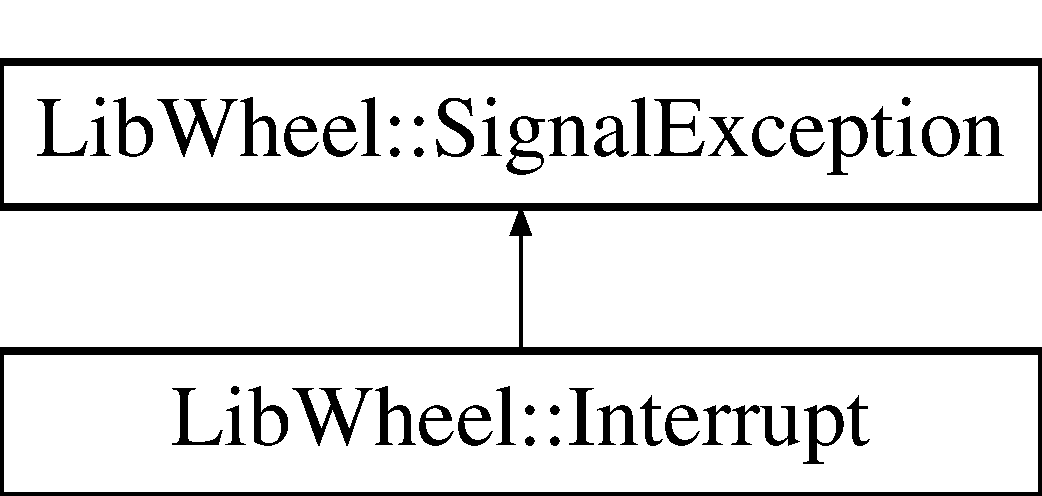
\includegraphics[height=2.000000cm]{classLibWheel_1_1Interrupt}
\end{center}
\end{figure}
\subsection*{\-Public \-Member \-Functions}
\begin{DoxyCompactItemize}
\item 
\hyperlink{classLibWheel_1_1Interrupt_a1aae086691cdc393008aaccab81c5adc}{\-Interrupt} ()  throw ()
\begin{DoxyCompactList}\small\item\em \-Constructor for \hyperlink{classLibWheel_1_1SignalException}{\-Signal\-Exception}. \end{DoxyCompactList}\item 
\hyperlink{classLibWheel_1_1Interrupt_a4679e7a5ebee81c4b619848d70026d50}{\-Interrupt} (const siginfo\-\_\-t $\ast$info)  throw ()
\begin{DoxyCompactList}\small\item\em \-Constructor for \hyperlink{classLibWheel_1_1SignalException}{\-Signal\-Exception}. \end{DoxyCompactList}\item 
const siginfo\-\_\-t $\ast$ \hyperlink{classLibWheel_1_1SignalException_a470409aa1db7608623c601c9bda573f4}{get\-Info} () const   throw ()
\begin{DoxyCompactList}\small\item\em \-Retrieve the details of a the signal represented by this \hyperlink{classLibWheel_1_1SignalException}{\-Signal\-Exception}. \end{DoxyCompactList}\item 
virtual const char $\ast$ \hyperlink{classLibWheel_1_1SignalException_a65ea3c23ec24f6448fb02624f9b039c2}{what} () const   throw ()
\begin{DoxyCompactList}\small\item\em \-Retrieve the description of the this exception. \end{DoxyCompactList}\item 
int \hyperlink{classLibWheel_1_1SignalException_a966b7c3d4054dd0a6c5121ae6d17d8cb}{get\-Signal\-Number} () const   throw ()
\begin{DoxyCompactList}\small\item\em \-Retrieve the signal number represented by this \hyperlink{classLibWheel_1_1SignalException}{\-Signal\-Exception}. \end{DoxyCompactList}\end{DoxyCompactItemize}
\subsection*{\-Static \-Public \-Attributes}
\begin{DoxyCompactItemize}
\item 
static const int \hyperlink{classLibWheel_1_1Interrupt_a73b379bb2504c68644a132100bc43c38}{signal\-Number} = \-S\-I\-G\-I\-N\-T
\begin{DoxyCompactList}\small\item\em \-Signal number for \hyperlink{classLibWheel_1_1Interrupt}{\-Interrupt}. \end{DoxyCompactList}\end{DoxyCompactItemize}


\subsection{\-Detailed \-Description}
\-Exception to be thrown in response to a \-S\-I\-G\-I\-N\-T. 

\subsection{\-Constructor \& \-Destructor \-Documentation}
\hypertarget{classLibWheel_1_1Interrupt_a1aae086691cdc393008aaccab81c5adc}{
\index{\-Lib\-Wheel\-::\-Interrupt@{\-Lib\-Wheel\-::\-Interrupt}!\-Interrupt@{\-Interrupt}}
\index{\-Interrupt@{\-Interrupt}!LibWheel::Interrupt@{\-Lib\-Wheel\-::\-Interrupt}}
\subsubsection[{\-Interrupt}]{\setlength{\rightskip}{0pt plus 5cm}\-Lib\-Wheel\-::\-Interrupt\-::\-Interrupt (
\begin{DoxyParamCaption}
{}
\end{DoxyParamCaption}
)  throw ()}}
\label{classLibWheel_1_1Interrupt_a1aae086691cdc393008aaccab81c5adc}


\-Constructor for \hyperlink{classLibWheel_1_1SignalException}{\-Signal\-Exception}. 

\-Initializes the base class (\hyperlink{classLibWheel_1_1SignalException}{\-Signal\-Exception}) with values appropriate for a \-S\-I\-G\-I\-N\-T. 

\-Definition at line 121 of file \-Signals.\-cpp.

\hypertarget{classLibWheel_1_1Interrupt_a4679e7a5ebee81c4b619848d70026d50}{
\index{\-Lib\-Wheel\-::\-Interrupt@{\-Lib\-Wheel\-::\-Interrupt}!\-Interrupt@{\-Interrupt}}
\index{\-Interrupt@{\-Interrupt}!LibWheel::Interrupt@{\-Lib\-Wheel\-::\-Interrupt}}
\subsubsection[{\-Interrupt}]{\setlength{\rightskip}{0pt plus 5cm}\-Lib\-Wheel\-::\-Interrupt\-::\-Interrupt (
\begin{DoxyParamCaption}
\item[{const siginfo\-\_\-t $\ast$}]{info}
\end{DoxyParamCaption}
)  throw ()\hspace{0.3cm}{\ttfamily  \mbox{[}explicit\mbox{]}}}}
\label{classLibWheel_1_1Interrupt_a4679e7a5ebee81c4b619848d70026d50}


\-Constructor for \hyperlink{classLibWheel_1_1SignalException}{\-Signal\-Exception}. 

\-Initializes the base class (\hyperlink{classLibWheel_1_1SignalException}{\-Signal\-Exception}) with values appropriate for a \-S\-I\-G\-I\-N\-T. 
\begin{DoxyParams}{\-Parameters}
{\em info} & \-Signal details. \\
\hline
\end{DoxyParams}


\-Definition at line 112 of file \-Signals.\-cpp.



\subsection{\-Member \-Function \-Documentation}
\hypertarget{classLibWheel_1_1SignalException_a470409aa1db7608623c601c9bda573f4}{
\index{\-Lib\-Wheel\-::\-Interrupt@{\-Lib\-Wheel\-::\-Interrupt}!get\-Info@{get\-Info}}
\index{get\-Info@{get\-Info}!LibWheel::Interrupt@{\-Lib\-Wheel\-::\-Interrupt}}
\subsubsection[{get\-Info}]{\setlength{\rightskip}{0pt plus 5cm}const siginfo\-\_\-t $\ast$ \-Lib\-Wheel\-::\-Signal\-Exception\-::get\-Info (
\begin{DoxyParamCaption}
{}
\end{DoxyParamCaption}
) const  throw ()\hspace{0.3cm}{\ttfamily  \mbox{[}inherited\mbox{]}}}}
\label{classLibWheel_1_1SignalException_a470409aa1db7608623c601c9bda573f4}


\-Retrieve the details of a the signal represented by this \hyperlink{classLibWheel_1_1SignalException}{\-Signal\-Exception}. 

\-See the man page for sigaction() for details on the contents of a {\ttfamily siginfo\-\_\-t}. \begin{DoxyReturn}{\-Returns}
\-A pointer to the details, or \-N\-U\-L\-L if they're not available. 
\end{DoxyReturn}


\-Definition at line 79 of file \-Signals.\-cpp.



\-References \-Lib\-Wheel\-::\-Signal\-Exception\-::siginfo.

\hypertarget{classLibWheel_1_1SignalException_a966b7c3d4054dd0a6c5121ae6d17d8cb}{
\index{\-Lib\-Wheel\-::\-Interrupt@{\-Lib\-Wheel\-::\-Interrupt}!get\-Signal\-Number@{get\-Signal\-Number}}
\index{get\-Signal\-Number@{get\-Signal\-Number}!LibWheel::Interrupt@{\-Lib\-Wheel\-::\-Interrupt}}
\subsubsection[{get\-Signal\-Number}]{\setlength{\rightskip}{0pt plus 5cm}int \-Lib\-Wheel\-::\-Signal\-Exception\-::get\-Signal\-Number (
\begin{DoxyParamCaption}
{}
\end{DoxyParamCaption}
) const  throw ()\hspace{0.3cm}{\ttfamily  \mbox{[}inherited\mbox{]}}}}
\label{classLibWheel_1_1SignalException_a966b7c3d4054dd0a6c5121ae6d17d8cb}


\-Retrieve the signal number represented by this \hyperlink{classLibWheel_1_1SignalException}{\-Signal\-Exception}. 

\begin{DoxyReturn}{\-Returns}
\-The signal number. 
\end{DoxyReturn}


\-Definition at line 101 of file \-Signals.\-cpp.



\-References \-Lib\-Wheel\-::\-Signal\-Exception\-::number.

\hypertarget{classLibWheel_1_1SignalException_a65ea3c23ec24f6448fb02624f9b039c2}{
\index{\-Lib\-Wheel\-::\-Interrupt@{\-Lib\-Wheel\-::\-Interrupt}!what@{what}}
\index{what@{what}!LibWheel::Interrupt@{\-Lib\-Wheel\-::\-Interrupt}}
\subsubsection[{what}]{\setlength{\rightskip}{0pt plus 5cm}const char $\ast$ \-Lib\-Wheel\-::\-Signal\-Exception\-::what (
\begin{DoxyParamCaption}
{}
\end{DoxyParamCaption}
) const  throw ()\hspace{0.3cm}{\ttfamily  \mbox{[}virtual, inherited\mbox{]}}}}
\label{classLibWheel_1_1SignalException_a65ea3c23ec24f6448fb02624f9b039c2}


\-Retrieve the description of the this exception. 

\begin{DoxyReturn}{\-Returns}
\-A pointer to the description, which may be an empty string. 
\end{DoxyReturn}


\-Definition at line 90 of file \-Signals.\-cpp.



\-References \-Lib\-Wheel\-::\-Signal\-Exception\-::description.



\subsection{\-Member \-Data \-Documentation}
\hypertarget{classLibWheel_1_1Interrupt_a73b379bb2504c68644a132100bc43c38}{
\index{\-Lib\-Wheel\-::\-Interrupt@{\-Lib\-Wheel\-::\-Interrupt}!signal\-Number@{signal\-Number}}
\index{signal\-Number@{signal\-Number}!LibWheel::Interrupt@{\-Lib\-Wheel\-::\-Interrupt}}
\subsubsection[{signal\-Number}]{\setlength{\rightskip}{0pt plus 5cm}const int {\bf \-Lib\-Wheel\-::\-Interrupt\-::signal\-Number} = \-S\-I\-G\-I\-N\-T\hspace{0.3cm}{\ttfamily  \mbox{[}static\mbox{]}}}}
\label{classLibWheel_1_1Interrupt_a73b379bb2504c68644a132100bc43c38}


\-Signal number for \hyperlink{classLibWheel_1_1Interrupt}{\-Interrupt}. 



\-Definition at line 64 of file \-Signals.\-hpp.



\-The documentation for this class was generated from the following files\-:\begin{DoxyCompactItemize}
\item 
\hyperlink{Signals_8hpp}{\-Signals.\-hpp}\item 
\hyperlink{Signals_8cpp}{\-Signals.\-cpp}\end{DoxyCompactItemize}

\hypertarget{classLibWheel_1_1IOException}{
\section{\-Lib\-Wheel\-:\-:\-I\-O\-Exception \-Class \-Reference}
\label{classLibWheel_1_1IOException}\index{\-Lib\-Wheel\-::\-I\-O\-Exception@{\-Lib\-Wheel\-::\-I\-O\-Exception}}
}


\-Exception thrown when an \-I/\-O error occurs.  




{\ttfamily \#include $<$util.\-hpp$>$}

\subsection*{\-Public \-Member \-Functions}
\begin{DoxyCompactItemize}
\item 
\hyperlink{classLibWheel_1_1IOException_ae3a8d18f4531e2ea26b30684cd6c9494}{\-I\-O\-Exception} (const std\-::string \&s)
\begin{DoxyCompactList}\small\item\em \-Constructor for \hyperlink{classLibWheel_1_1IOException}{\-I\-O\-Exception}. \end{DoxyCompactList}\end{DoxyCompactItemize}


\subsection{\-Detailed \-Description}
\-Exception thrown when an \-I/\-O error occurs. 

\subsection{\-Constructor \& \-Destructor \-Documentation}
\hypertarget{classLibWheel_1_1IOException_ae3a8d18f4531e2ea26b30684cd6c9494}{
\index{\-Lib\-Wheel\-::\-I\-O\-Exception@{\-Lib\-Wheel\-::\-I\-O\-Exception}!\-I\-O\-Exception@{\-I\-O\-Exception}}
\index{\-I\-O\-Exception@{\-I\-O\-Exception}!LibWheel::IOException@{\-Lib\-Wheel\-::\-I\-O\-Exception}}
\subsubsection[{\-I\-O\-Exception}]{\setlength{\rightskip}{0pt plus 5cm}\-Lib\-Wheel\-::\-I\-O\-Exception\-::\-I\-O\-Exception (
\begin{DoxyParamCaption}
\item[{const std\-::string \&}]{s}
\end{DoxyParamCaption}
)}}
\label{classLibWheel_1_1IOException_ae3a8d18f4531e2ea26b30684cd6c9494}


\-Constructor for \hyperlink{classLibWheel_1_1IOException}{\-I\-O\-Exception}. 


\begin{DoxyParams}{\-Parameters}
{\em s} & \-A string describing the reason for throwing the exception. \\
\hline
\end{DoxyParams}


\-Definition at line 138 of file util.\-cpp.



\-The documentation for this class was generated from the following files\-:\begin{DoxyCompactItemize}
\item 
\hyperlink{util_8hpp}{util.\-hpp}\item 
\hyperlink{util_8cpp}{util.\-cpp}\end{DoxyCompactItemize}

\hypertarget{classIPQ_1_1IpqException}{
\section{\-I\-P\-Q\-:\-:\-Ipq\-Exception \-Class \-Reference}
\label{classIPQ_1_1IpqException}\index{\-I\-P\-Q\-::\-Ipq\-Exception@{\-I\-P\-Q\-::\-Ipq\-Exception}}
}


\-Base class for exceptions thrown by \hyperlink{namespaceIPQ}{\-I\-P\-Q} methods.  




{\ttfamily \#include $<$\-I\-P\-Q.\-hpp$>$}

\subsection*{\-Public \-Member \-Functions}
\begin{DoxyCompactItemize}
\item 
\hyperlink{classIPQ_1_1IpqException_a74679f280b296b67cec046424d7e0502}{\-Ipq\-Exception} (const std\-::string \&d)
\begin{DoxyCompactList}\small\item\em \-Constructor for \hyperlink{classIPQ_1_1IpqException}{\-Ipq\-Exception}. \end{DoxyCompactList}\item 
virtual \hyperlink{classIPQ_1_1IpqException_a4f2a79d4f40102b4ce6c5f8b6f62eff2}{$\sim$\-Ipq\-Exception} ()  throw ()
\begin{DoxyCompactList}\small\item\em \-Destructor for \hyperlink{classIPQ_1_1IpqException}{\-Ipq\-Exception}. \end{DoxyCompactList}\end{DoxyCompactItemize}


\subsection{\-Detailed \-Description}
\-Base class for exceptions thrown by \hyperlink{namespaceIPQ}{\-I\-P\-Q} methods. 

\subsection{\-Constructor \& \-Destructor \-Documentation}
\hypertarget{classIPQ_1_1IpqException_a74679f280b296b67cec046424d7e0502}{
\index{\-I\-P\-Q\-::\-Ipq\-Exception@{\-I\-P\-Q\-::\-Ipq\-Exception}!\-Ipq\-Exception@{\-Ipq\-Exception}}
\index{\-Ipq\-Exception@{\-Ipq\-Exception}!IPQ::IpqException@{\-I\-P\-Q\-::\-Ipq\-Exception}}
\subsubsection[{\-Ipq\-Exception}]{\setlength{\rightskip}{0pt plus 5cm}\-I\-P\-Q\-::\-Ipq\-Exception\-::\-Ipq\-Exception (
\begin{DoxyParamCaption}
\item[{const std\-::string \&}]{d}
\end{DoxyParamCaption}
)}}
\label{classIPQ_1_1IpqException_a74679f280b296b67cec046424d7e0502}


\-Constructor for \hyperlink{classIPQ_1_1IpqException}{\-Ipq\-Exception}. 



\-Definition at line 82 of file \-I\-P\-Q.\-cpp.

\hypertarget{classIPQ_1_1IpqException_a4f2a79d4f40102b4ce6c5f8b6f62eff2}{
\index{\-I\-P\-Q\-::\-Ipq\-Exception@{\-I\-P\-Q\-::\-Ipq\-Exception}!$\sim$\-Ipq\-Exception@{$\sim$\-Ipq\-Exception}}
\index{$\sim$\-Ipq\-Exception@{$\sim$\-Ipq\-Exception}!IPQ::IpqException@{\-I\-P\-Q\-::\-Ipq\-Exception}}
\subsubsection[{$\sim$\-Ipq\-Exception}]{\setlength{\rightskip}{0pt plus 5cm}\-I\-P\-Q\-::\-Ipq\-Exception\-::$\sim$\-Ipq\-Exception (
\begin{DoxyParamCaption}
{}
\end{DoxyParamCaption}
)  throw ()\hspace{0.3cm}{\ttfamily  \mbox{[}virtual\mbox{]}}}}
\label{classIPQ_1_1IpqException_a4f2a79d4f40102b4ce6c5f8b6f62eff2}


\-Destructor for \hyperlink{classIPQ_1_1IpqException}{\-Ipq\-Exception}. 



\-Definition at line 90 of file \-I\-P\-Q.\-cpp.



\-The documentation for this class was generated from the following files\-:\begin{DoxyCompactItemize}
\item 
\hyperlink{IPQ_8hpp}{\-I\-P\-Q.\-hpp}\item 
\hyperlink{IPQ_8cpp}{\-I\-P\-Q.\-cpp}\end{DoxyCompactItemize}

\hypertarget{classIPQ_1_1IpqIpPacket}{
\section{\-I\-P\-Q\-:\-:\-Ipq\-Ip\-Packet \-Class \-Reference}
\label{classIPQ_1_1IpqIpPacket}\index{\-I\-P\-Q\-::\-Ipq\-Ip\-Packet@{\-I\-P\-Q\-::\-Ipq\-Ip\-Packet}}
}


\-A complete \-I\-Pv4 packet received via \hyperlink{classIPQ_1_1IpqSocket}{\-Ipq\-Socket}.  




{\ttfamily \#include $<$\-I\-P\-Q.\-hpp$>$}

\-Inheritance diagram for \-I\-P\-Q\-:\-:\-Ipq\-Ip\-Packet\-:\begin{figure}[H]
\begin{center}
\leavevmode
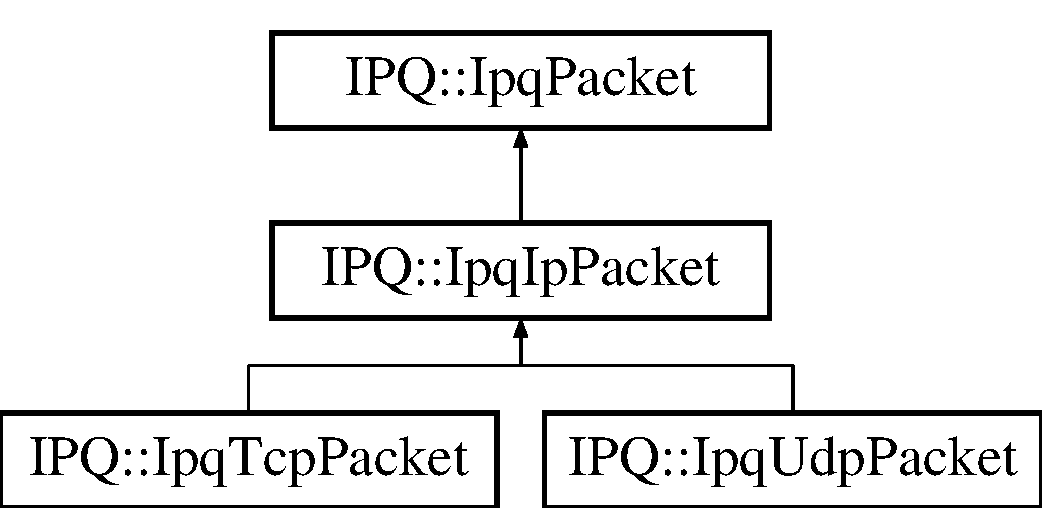
\includegraphics[height=3.000000cm]{classIPQ_1_1IpqIpPacket}
\end{center}
\end{figure}
\subsection*{\-Public \-Member \-Functions}
\begin{DoxyCompactItemize}
\item 
in\-\_\-addr\-\_\-t \hyperlink{classIPQ_1_1IpqIpPacket_a4708c5a987eb9796566e2b3bdd072589}{get\-Ip\-Source} () const 
\begin{DoxyCompactList}\small\item\em \-Retrieve the source \-I\-P address of a packet. \end{DoxyCompactList}\item 
in\-\_\-addr\-\_\-t \hyperlink{classIPQ_1_1IpqIpPacket_a056bedcbf7998452d147f2d2ef68b611}{get\-Ip\-Dest} () const 
\begin{DoxyCompactList}\small\item\em \-Retrieve the destination \-I\-P address of a packet. \end{DoxyCompactList}\item 
boost\-::uint8\-\_\-t \hyperlink{classIPQ_1_1IpqIpPacket_aefa78bb7a89a337bb0c1d88c02d6d5cd}{get\-Protocol} () const 
\begin{DoxyCompactList}\small\item\em \-Retrieve the encapsulated protocol number of a packet. \end{DoxyCompactList}\item 
boost\-::uint16\-\_\-t \hyperlink{classIPQ_1_1IpqIpPacket_a937be4034dafdce171b7e90ae14f09d4}{get\-Id} () const 
\begin{DoxyCompactList}\small\item\em \-Retrieve the \-I\-P \-I\-D of a packet. \end{DoxyCompactList}\item 
boost\-::uint16\-\_\-t \hyperlink{classIPQ_1_1IpqIpPacket_a97e6e13ede2c6c6f028ee0eb1130600b}{get\-Frag\-Offset} () const 
\begin{DoxyCompactList}\small\item\em \-Retrieve the fragment offset of a packet, in bytes. \end{DoxyCompactList}\item 
bool \hyperlink{classIPQ_1_1IpqIpPacket_a76e0d09916fc816df3dab46cb29d479f}{get\-More\-Frags} () const 
\begin{DoxyCompactList}\small\item\em \-Retrieve the \char`\"{}more fragments to follow\char`\"{} flag of a packet. \end{DoxyCompactList}\item 
struct iphdr \& \hyperlink{classIPQ_1_1IpqIpPacket_abf46954191d96b4e2fe136f79ba6c8ac}{get\-Ip\-Header} () const 
\begin{DoxyCompactList}\small\item\em \-Retrieve the complete \-I\-P header of a packet. \end{DoxyCompactList}\item 
struct iphdr \& \hyperlink{classIPQ_1_1IpqIpPacket_aa6e89b7927e748d00b9562e85192b492}{get\-Ip\-Header} ()
\begin{DoxyCompactList}\small\item\em \-Retrieve the complete \-I\-P header of a packet. \end{DoxyCompactList}\item 
const boost\-::uint8\-\_\-t $\ast$ \hyperlink{classIPQ_1_1IpqIpPacket_adc020ff0aceeba0577e4bb90dcc6f86f}{get\-Ip\-Payload} (std\-::size\-\_\-t \&size) const 
\begin{DoxyCompactList}\small\item\em \-Retrive the \-I\-P payload of a packet. \end{DoxyCompactList}\item 
boost\-::uint8\-\_\-t $\ast$ \hyperlink{classIPQ_1_1IpqIpPacket_a47343dd1a4fc52c8fda6de4aa313a688}{get\-Ip\-Payload} (std\-::size\-\_\-t \&size)
\begin{DoxyCompactList}\small\item\em \-Retrive the \-I\-P payload of a packet. \end{DoxyCompactList}\item 
virtual void \hyperlink{classIPQ_1_1IpqIpPacket_a5ddc175ec8c4bc8c7bab3baee12909f0}{print} (std\-::ostream \&out) const 
\begin{DoxyCompactList}\small\item\em \-Print an \-I\-P packet to stdout in an easy-\/to-\/read format. \end{DoxyCompactList}\item 
virtual \hyperlink{classIPQ_1_1IpqIpPacket_a13e93bcb4fa2dc3fdc4ec122c1666574}{$\sim$\-Ipq\-Ip\-Packet} ()
\begin{DoxyCompactList}\small\item\em \-Destructor for \hyperlink{classIPQ_1_1IpqIpPacket}{\-Ipq\-Ip\-Packet}. \end{DoxyCompactList}\item 
unsigned long \hyperlink{classIPQ_1_1IpqPacket_ac3cbbe2b61e12730ffe231fa19c96e5a}{get\-Nf\-Id} () const 
\begin{DoxyCompactList}\small\item\em \-Retrieve the \-Netfilter \-I\-D of a packet. \end{DoxyCompactList}\item 
unsigned long \hyperlink{classIPQ_1_1IpqPacket_ab97f0a4348e53cb69ed1da74e422dc78}{get\-Nf\-Mark} () const 
\begin{DoxyCompactList}\small\item\em \-Retrieve the \-Netfilter mark value of a packet. \end{DoxyCompactList}\item 
void \hyperlink{classIPQ_1_1IpqPacket_a430ce4f89e651724efdf56c9c1b1647e}{get\-Timestamp} (struct timeval \&time) const 
\begin{DoxyCompactList}\small\item\em \-Retrieve the arrival time of a packet. \end{DoxyCompactList}\item 
unsigned \hyperlink{classIPQ_1_1IpqPacket_ae13884fedce165702f4b71e0e4d93c0b}{get\-Nf\-Hook} () const 
\begin{DoxyCompactList}\small\item\em \-Retrieve the number of the \-Netfilter hook on which the packet arrived. \end{DoxyCompactList}\item 
const char(\& \hyperlink{classIPQ_1_1IpqPacket_a4cf04ca5da28410f27d87edefd679532}{get\-Indev\-Name} () const)\mbox{[}\-I\-F\-N\-A\-M\-S\-I\-Z\mbox{]}
\begin{DoxyCompactList}\small\item\em \-Retrieve the name of the interface on which the packet arrived, if available. \end{DoxyCompactList}\item 
const char(\& \hyperlink{classIPQ_1_1IpqPacket_a46dced8057de3bba7abfaaa63d7afcd4}{get\-Outdev\-Name} () const)\mbox{[}\-I\-F\-N\-A\-M\-S\-I\-Z\mbox{]}
\begin{DoxyCompactList}\small\item\em \-Retrieve the name of the interface on which the packet will leave, if available. \end{DoxyCompactList}\item 
unsigned short \hyperlink{classIPQ_1_1IpqPacket_ae150e294f043f4c699231a85d3b1ae0f}{get\-Hw\-Protocol} () const 
\begin{DoxyCompactList}\small\item\em \-Retrieve the hardware protocol number of the packet. \end{DoxyCompactList}\item 
unsigned short \hyperlink{classIPQ_1_1IpqPacket_ab6b76b146111c7ad11b96e87efe6634c}{get\-Hw\-Type} () const 
\begin{DoxyCompactList}\small\item\em \-Retrieve the hardware type on which the packet arrived. \end{DoxyCompactList}\item 
const unsigned char(\& \hyperlink{classIPQ_1_1IpqPacket_a8582ae732d6b66ca1f5201994159a84a}{get\-Hw\-Source} (unsigned short \&addrlen) const)\mbox{[}8\mbox{]}
\begin{DoxyCompactList}\small\item\em \-Retrieve the source hardware address of the packet. \end{DoxyCompactList}\item 
const boost\-::uint8\-\_\-t $\ast$ \hyperlink{classIPQ_1_1IpqPacket_a6dd7baeec66082658d882bff8862eb6c}{get\-Packet} (std\-::size\-\_\-t \&size) const 
\begin{DoxyCompactList}\small\item\em \-Retrieve the packet. \end{DoxyCompactList}\item 
boost\-::uint8\-\_\-t $\ast$ \hyperlink{classIPQ_1_1IpqPacket_a0bf3344a9eed5e2f6bc20890ffffe26e}{get\-Packet} (std\-::size\-\_\-t \&size)
\begin{DoxyCompactList}\small\item\em \-Retrieve the packet. \end{DoxyCompactList}\end{DoxyCompactItemize}
\subsection*{\-Protected \-Member \-Functions}
\begin{DoxyCompactItemize}
\item 
\hyperlink{classIPQ_1_1IpqIpPacket_a1517b15b34742a3c2469ba7c5ed5ed01}{\-Ipq\-Ip\-Packet} (\hyperlink{classLibWheel_1_1auto__array}{\-Lib\-Wheel\-::auto\-\_\-array}$<$ boost\-::uint8\-\_\-t $>$ buf, std\-::size\-\_\-t buflen)
\begin{DoxyCompactList}\small\item\em \-Constructor for \hyperlink{classIPQ_1_1IpqIpPacket}{\-Ipq\-Ip\-Packet}. \end{DoxyCompactList}\item 
struct iphdr \& \hyperlink{classIPQ_1_1IpqIpPacket_a6be0afa1f616cbe7722ef817a65e24dc}{do\-Get\-Ip\-Header} () const 
\begin{DoxyCompactList}\small\item\em \-Retrieve the complete \-I\-P header of a packet. \end{DoxyCompactList}\item 
boost\-::uint8\-\_\-t $\ast$ \hyperlink{classIPQ_1_1IpqIpPacket_ab78709e0712a1912d19114f815407303}{do\-Get\-Ip\-Payload} (std\-::size\-\_\-t \&size) const 
\begin{DoxyCompactList}\small\item\em \-Retrive the \-I\-P payload of a packet. \end{DoxyCompactList}\item 
virtual void \hyperlink{classIPQ_1_1IpqIpPacket_a4c2c0ccd36ef921f6632b26ebd524b90}{update\-Checksums} ()
\begin{DoxyCompactList}\small\item\em \-Update the checksums on an \-I\-P packet. \end{DoxyCompactList}\item 
boost\-::uint8\-\_\-t $\ast$ \hyperlink{classIPQ_1_1IpqPacket_a7b8f489a9cec36058eaee43f6566a999}{do\-Get\-Packet} (std\-::size\-\_\-t \&size) const 
\begin{DoxyCompactList}\small\item\em \-Retrieve the packet. \end{DoxyCompactList}\end{DoxyCompactItemize}
\subsection*{\-Static \-Protected \-Member \-Functions}
\begin{DoxyCompactItemize}
\item 
static \hyperlink{classIPQ_1_1IpqPacket}{\-Ipq\-Packet} $\ast$ \hyperlink{classIPQ_1_1IpqPacket_adf6099052730113814e9fe7312ec7b8c}{create\-Packet} (\hyperlink{classLibWheel_1_1auto__array}{\-Lib\-Wheel\-::auto\-\_\-array}$<$ boost\-::uint8\-\_\-t $>$ buf, std\-::size\-\_\-t buflen)
\begin{DoxyCompactList}\small\item\em \-Create an \hyperlink{classIPQ_1_1IpqPacket}{\-Ipq\-Packet} or one of its subclasses from a libipq packet message. \end{DoxyCompactList}\end{DoxyCompactItemize}
\subsection*{\-Protected \-Attributes}
\begin{DoxyCompactItemize}
\item 
\hyperlink{classLibWheel_1_1auto__array}{\-Lib\-Wheel\-::auto\-\_\-array}\*
$<$ boost\-::uint8\-\_\-t $>$ \hyperlink{classIPQ_1_1IpqPacket_a2bdf247f13a3e9f86e9e3846e6a9cb45}{packet}
\begin{DoxyCompactList}\small\item\em \-The packet message received from kernelspace. \end{DoxyCompactList}\item 
std\-::size\-\_\-t \hyperlink{classIPQ_1_1IpqPacket_a9b448a070c5ae499e32d2af5a190b86d}{packet\-Len}
\begin{DoxyCompactList}\small\item\em the length of the packet message in \hyperlink{classIPQ_1_1IpqPacket_a2bdf247f13a3e9f86e9e3846e6a9cb45}{\-Ipq\-Packet\-::packet}, in bytes. \end{DoxyCompactList}\item 
bool \hyperlink{classIPQ_1_1IpqPacket_a00acebf51531043a8536f20bb9412d61}{dirty}
\begin{DoxyCompactList}\small\item\em {\bfseries true} if the packet has been modified but checksums have not been updated; {\bfseries false} otherwise. \end{DoxyCompactList}\end{DoxyCompactItemize}
\subsection*{\-Friends}
\begin{DoxyCompactItemize}
\item 
\hyperlink{classIPQ_1_1IpqPacket}{\-Ipq\-Packet} $\ast$ \hyperlink{classIPQ_1_1IpqIpPacket_af2019ef9442b13f8da0f53a082a9b308}{\-Ipq\-Packet\-::create\-Packet} (\hyperlink{classLibWheel_1_1auto__array}{\-Lib\-Wheel\-::auto\-\_\-array}$<$ boost\-::uint8\-\_\-t $>$, std\-::size\-\_\-t)
\begin{DoxyCompactList}\small\item\em \-Allow \-Ipq\-Socket\-::create\-Packet() to access the contstructor. \end{DoxyCompactList}\end{DoxyCompactItemize}


\subsection{\-Detailed \-Description}
\-A complete \-I\-Pv4 packet received via \hyperlink{classIPQ_1_1IpqSocket}{\-Ipq\-Socket}. 

\-Contains \-I\-P header fields and the \-I\-P payload. \begin{DoxyNote}{\-Note}
\-This class does not reassemble \-I\-P fragments. 
\end{DoxyNote}


\subsection{\-Constructor \& \-Destructor \-Documentation}
\hypertarget{classIPQ_1_1IpqIpPacket_a13e93bcb4fa2dc3fdc4ec122c1666574}{
\index{\-I\-P\-Q\-::\-Ipq\-Ip\-Packet@{\-I\-P\-Q\-::\-Ipq\-Ip\-Packet}!$\sim$\-Ipq\-Ip\-Packet@{$\sim$\-Ipq\-Ip\-Packet}}
\index{$\sim$\-Ipq\-Ip\-Packet@{$\sim$\-Ipq\-Ip\-Packet}!IPQ::IpqIpPacket@{\-I\-P\-Q\-::\-Ipq\-Ip\-Packet}}
\subsubsection[{$\sim$\-Ipq\-Ip\-Packet}]{\setlength{\rightskip}{0pt plus 5cm}\-I\-P\-Q\-::\-Ipq\-Ip\-Packet\-::$\sim$\-Ipq\-Ip\-Packet (
\begin{DoxyParamCaption}
{}
\end{DoxyParamCaption}
)\hspace{0.3cm}{\ttfamily  \mbox{[}virtual\mbox{]}}}}
\label{classIPQ_1_1IpqIpPacket_a13e93bcb4fa2dc3fdc4ec122c1666574}


\-Destructor for \hyperlink{classIPQ_1_1IpqIpPacket}{\-Ipq\-Ip\-Packet}. 



\-Definition at line 910 of file \-I\-P\-Q.\-cpp.

\hypertarget{classIPQ_1_1IpqIpPacket_a1517b15b34742a3c2469ba7c5ed5ed01}{
\index{\-I\-P\-Q\-::\-Ipq\-Ip\-Packet@{\-I\-P\-Q\-::\-Ipq\-Ip\-Packet}!\-Ipq\-Ip\-Packet@{\-Ipq\-Ip\-Packet}}
\index{\-Ipq\-Ip\-Packet@{\-Ipq\-Ip\-Packet}!IPQ::IpqIpPacket@{\-I\-P\-Q\-::\-Ipq\-Ip\-Packet}}
\subsubsection[{\-Ipq\-Ip\-Packet}]{\setlength{\rightskip}{0pt plus 5cm}\-I\-P\-Q\-::\-Ipq\-Ip\-Packet\-::\-Ipq\-Ip\-Packet (
\begin{DoxyParamCaption}
\item[{{\bf \-Lib\-Wheel\-::auto\-\_\-array}$<$ boost\-::uint8\-\_\-t $>$}]{buf, }
\item[{std\-::size\-\_\-t}]{buflen}
\end{DoxyParamCaption}
)\hspace{0.3cm}{\ttfamily  \mbox{[}protected\mbox{]}}}}
\label{classIPQ_1_1IpqIpPacket_a1517b15b34742a3c2469ba7c5ed5ed01}


\-Constructor for \hyperlink{classIPQ_1_1IpqIpPacket}{\-Ipq\-Ip\-Packet}. 

\-Initializes an \hyperlink{classIPQ_1_1IpqIpPacket}{\-Ipq\-Ip\-Packet} from a libipq packet message. 

\-Definition at line 918 of file \-I\-P\-Q.\-cpp.



\subsection{\-Member \-Function \-Documentation}
\hypertarget{classIPQ_1_1IpqPacket_adf6099052730113814e9fe7312ec7b8c}{
\index{\-I\-P\-Q\-::\-Ipq\-Ip\-Packet@{\-I\-P\-Q\-::\-Ipq\-Ip\-Packet}!create\-Packet@{create\-Packet}}
\index{create\-Packet@{create\-Packet}!IPQ::IpqIpPacket@{\-I\-P\-Q\-::\-Ipq\-Ip\-Packet}}
\subsubsection[{create\-Packet}]{\setlength{\rightskip}{0pt plus 5cm}{\bf \-Ipq\-Packet} $\ast$ \-I\-P\-Q\-::\-Ipq\-Packet\-::create\-Packet (
\begin{DoxyParamCaption}
\item[{{\bf \-Lib\-Wheel\-::auto\-\_\-array}$<$ boost\-::uint8\-\_\-t $>$}]{buf, }
\item[{std\-::size\-\_\-t}]{buflen}
\end{DoxyParamCaption}
)\hspace{0.3cm}{\ttfamily  \mbox{[}static, protected, inherited\mbox{]}}}}
\label{classIPQ_1_1IpqPacket_adf6099052730113814e9fe7312ec7b8c}


\-Create an \hyperlink{classIPQ_1_1IpqPacket}{\-Ipq\-Packet} or one of its subclasses from a libipq packet message. 

\-A packet will be deemed to be an \-I\-Pv4 packet if it has a full \-I\-Pv4 header and the data length indicated by the header matches the packet's length. \-A packet will be deemed to be a \-T\-C\-P or \-U\-D\-P packet if it is an \-I\-Pv4 packet and it has a full \-T\-C\-P or \-U\-D\-P header. \begin{DoxyReturn}{\-Returns}
\-A pointer to a dynamically-\/allocated \hyperlink{classIPQ_1_1IpqPacket}{\-Ipq\-Packet}, or one of its subclasses. \-This pointer must be freed using {\bfseries delete}, and a verdict should be set on it using \hyperlink{classIPQ_1_1IpqSocket_a53e0f4e45363cbcd919a2d96ee7cf0a8}{\-Ipq\-Socket\-::send\-Response()}. 
\end{DoxyReturn}


\-Definition at line 731 of file \-I\-P\-Q.\-cpp.



\-References \-Lib\-Wheel\-::auto\-\_\-array\-::get(), and \-I\-P\-Q\-::\-Ipq\-Packet\-::\-Ipq\-Packet().



\-Referenced by \-I\-P\-Q\-::\-Ipq\-Socket\-::recv\-Packet().

\hypertarget{classIPQ_1_1IpqIpPacket_a6be0afa1f616cbe7722ef817a65e24dc}{
\index{\-I\-P\-Q\-::\-Ipq\-Ip\-Packet@{\-I\-P\-Q\-::\-Ipq\-Ip\-Packet}!do\-Get\-Ip\-Header@{do\-Get\-Ip\-Header}}
\index{do\-Get\-Ip\-Header@{do\-Get\-Ip\-Header}!IPQ::IpqIpPacket@{\-I\-P\-Q\-::\-Ipq\-Ip\-Packet}}
\subsubsection[{do\-Get\-Ip\-Header}]{\setlength{\rightskip}{0pt plus 5cm}struct iphdr \& \-I\-P\-Q\-::\-Ipq\-Ip\-Packet\-::do\-Get\-Ip\-Header (
\begin{DoxyParamCaption}
{}
\end{DoxyParamCaption}
) const\hspace{0.3cm}{\ttfamily  \mbox{[}read, protected\mbox{]}}}}
\label{classIPQ_1_1IpqIpPacket_a6be0afa1f616cbe7722ef817a65e24dc}


\-Retrieve the complete \-I\-P header of a packet. 

\-A reference to the packet's \-I\-P header. 

\-Definition at line 928 of file \-I\-P\-Q.\-cpp.



\-References \-I\-P\-Q\-::\-Ipq\-Packet\-::packet, and \-Lib\-Wheel\-::auto\-\_\-array\-::get().



\-Referenced by get\-Ip\-Header().

\hypertarget{classIPQ_1_1IpqIpPacket_ab78709e0712a1912d19114f815407303}{
\index{\-I\-P\-Q\-::\-Ipq\-Ip\-Packet@{\-I\-P\-Q\-::\-Ipq\-Ip\-Packet}!do\-Get\-Ip\-Payload@{do\-Get\-Ip\-Payload}}
\index{do\-Get\-Ip\-Payload@{do\-Get\-Ip\-Payload}!IPQ::IpqIpPacket@{\-I\-P\-Q\-::\-Ipq\-Ip\-Packet}}
\subsubsection[{do\-Get\-Ip\-Payload}]{\setlength{\rightskip}{0pt plus 5cm}boost\-::uint8\-\_\-t $\ast$ \-I\-P\-Q\-::\-Ipq\-Ip\-Packet\-::do\-Get\-Ip\-Payload (
\begin{DoxyParamCaption}
\item[{std\-::size\-\_\-t \&}]{size}
\end{DoxyParamCaption}
) const\hspace{0.3cm}{\ttfamily  \mbox{[}protected\mbox{]}}}}
\label{classIPQ_1_1IpqIpPacket_ab78709e0712a1912d19114f815407303}


\-Retrive the \-I\-P payload of a packet. 


\begin{DoxyParams}[1]{\-Parameters}
\mbox{\tt out}  & {\em size} & \-A reference to a location to store the packet's \-I\-P payload size, in bytes.. \\
\hline
\end{DoxyParams}
\begin{DoxyReturn}{\-Returns}
\-A const pointer to the packet's \-I\-P payload. 
\end{DoxyReturn}


\-Definition at line 941 of file \-I\-P\-Q.\-cpp.



\-References \-I\-P\-Q\-::\-Ipq\-Packet\-::packet, and \-Lib\-Wheel\-::auto\-\_\-array\-::get().



\-Referenced by get\-Ip\-Payload().

\hypertarget{classIPQ_1_1IpqPacket_a7b8f489a9cec36058eaee43f6566a999}{
\index{\-I\-P\-Q\-::\-Ipq\-Ip\-Packet@{\-I\-P\-Q\-::\-Ipq\-Ip\-Packet}!do\-Get\-Packet@{do\-Get\-Packet}}
\index{do\-Get\-Packet@{do\-Get\-Packet}!IPQ::IpqIpPacket@{\-I\-P\-Q\-::\-Ipq\-Ip\-Packet}}
\subsubsection[{do\-Get\-Packet}]{\setlength{\rightskip}{0pt plus 5cm}boost\-::uint8\-\_\-t $\ast$ \-I\-P\-Q\-::\-Ipq\-Packet\-::do\-Get\-Packet (
\begin{DoxyParamCaption}
\item[{std\-::size\-\_\-t \&}]{size}
\end{DoxyParamCaption}
) const\hspace{0.3cm}{\ttfamily  \mbox{[}protected, inherited\mbox{]}}}}
\label{classIPQ_1_1IpqPacket_a7b8f489a9cec36058eaee43f6566a999}


\-Retrieve the packet. 

\-It will only be available if the copy mode on the libipq handle used to receive it was \hyperlink{classIPQ_1_1IpqSocket_afee6d75480079906ecf6544f8467e0ccafc1e90369658a807b2c970d3e15b01d4}{\-Ipq\-Socket\-::\-P\-A\-C\-K\-E\-T} and the copy range was greater than zero. 
\begin{DoxyParams}[1]{\-Parameters}
\mbox{\tt out}  & {\em size} & \-A reference to a location to write the length of the payload, in bytes. \\
\hline
\end{DoxyParams}
\begin{DoxyReturn}{\-Returns}
\-A pointer to the packet. 
\end{DoxyReturn}


\-Definition at line 703 of file \-I\-P\-Q.\-cpp.



\-References \-I\-P\-Q\-::\-Ipq\-Packet\-::packet, and \-Lib\-Wheel\-::auto\-\_\-array\-::get().



\-Referenced by \-I\-P\-Q\-::\-Ipq\-Packet\-::get\-Packet().

\hypertarget{classIPQ_1_1IpqIpPacket_a97e6e13ede2c6c6f028ee0eb1130600b}{
\index{\-I\-P\-Q\-::\-Ipq\-Ip\-Packet@{\-I\-P\-Q\-::\-Ipq\-Ip\-Packet}!get\-Frag\-Offset@{get\-Frag\-Offset}}
\index{get\-Frag\-Offset@{get\-Frag\-Offset}!IPQ::IpqIpPacket@{\-I\-P\-Q\-::\-Ipq\-Ip\-Packet}}
\subsubsection[{get\-Frag\-Offset}]{\setlength{\rightskip}{0pt plus 5cm}boost\-::uint16\-\_\-t \-I\-P\-Q\-::\-Ipq\-Ip\-Packet\-::get\-Frag\-Offset (
\begin{DoxyParamCaption}
{}
\end{DoxyParamCaption}
) const}}
\label{classIPQ_1_1IpqIpPacket_a97e6e13ede2c6c6f028ee0eb1130600b}


\-Retrieve the fragment offset of a packet, in bytes. 

\-If not zero, then this is a non-\/leading fragment. \begin{DoxyReturn}{\-Returns}
\-The packet's fragment offset. 
\end{DoxyReturn}


\-Definition at line 817 of file \-I\-P\-Q.\-cpp.



\-References get\-Ip\-Header().



\-Referenced by print(), and \-N\-E\-R\-D\-::\-Connection\-Server\-::handle\-Packet().

\hypertarget{classIPQ_1_1IpqPacket_ae150e294f043f4c699231a85d3b1ae0f}{
\index{\-I\-P\-Q\-::\-Ipq\-Ip\-Packet@{\-I\-P\-Q\-::\-Ipq\-Ip\-Packet}!get\-Hw\-Protocol@{get\-Hw\-Protocol}}
\index{get\-Hw\-Protocol@{get\-Hw\-Protocol}!IPQ::IpqIpPacket@{\-I\-P\-Q\-::\-Ipq\-Ip\-Packet}}
\subsubsection[{get\-Hw\-Protocol}]{\setlength{\rightskip}{0pt plus 5cm}unsigned short \-I\-P\-Q\-::\-Ipq\-Packet\-::get\-Hw\-Protocol (
\begin{DoxyParamCaption}
{}
\end{DoxyParamCaption}
) const\hspace{0.3cm}{\ttfamily  \mbox{[}inherited\mbox{]}}}}
\label{classIPQ_1_1IpqPacket_ae150e294f043f4c699231a85d3b1ae0f}


\-Retrieve the hardware protocol number of the packet. 

\begin{DoxyReturn}{\-Returns}
\-The packet's hardware protocol number. 
\end{DoxyReturn}


\-Definition at line 585 of file \-I\-P\-Q.\-cpp.



\-References \-I\-P\-Q\-::\-Ipq\-Packet\-::packet, and \-Lib\-Wheel\-::auto\-\_\-array\-::get().



\-Referenced by \-I\-P\-Q\-::\-Ipq\-Packet\-::print().

\hypertarget{classIPQ_1_1IpqPacket_a8582ae732d6b66ca1f5201994159a84a}{
\index{\-I\-P\-Q\-::\-Ipq\-Ip\-Packet@{\-I\-P\-Q\-::\-Ipq\-Ip\-Packet}!get\-Hw\-Source@{get\-Hw\-Source}}
\index{get\-Hw\-Source@{get\-Hw\-Source}!IPQ::IpqIpPacket@{\-I\-P\-Q\-::\-Ipq\-Ip\-Packet}}
\subsubsection[{get\-Hw\-Source}]{\setlength{\rightskip}{0pt plus 5cm}const unsigned char(\& \-I\-P\-Q\-::\-Ipq\-Packet\-::get\-Hw\-Source (
\begin{DoxyParamCaption}
\item[{unsigned short \&}]{addrlen}
\end{DoxyParamCaption}
))\mbox{[}8\mbox{]}\hspace{0.3cm}{\ttfamily  \mbox{[}inherited\mbox{]}}}}
\label{classIPQ_1_1IpqPacket_a8582ae732d6b66ca1f5201994159a84a}


\-Retrieve the source hardware address of the packet. 


\begin{DoxyParams}[1]{\-Parameters}
\mbox{\tt out}  & {\em addrlen} & \-A reference to a location to write the actual length of the address, in bytes. \\
\hline
\end{DoxyParams}
\begin{DoxyReturn}{\-Returns}
\-A reference to the packet's source hardware address. 
\end{DoxyReturn}


\-Definition at line 608 of file \-I\-P\-Q.\-cpp.



\-Referenced by \-I\-P\-Q\-::\-Ipq\-Packet\-::print().

\hypertarget{classIPQ_1_1IpqPacket_ab6b76b146111c7ad11b96e87efe6634c}{
\index{\-I\-P\-Q\-::\-Ipq\-Ip\-Packet@{\-I\-P\-Q\-::\-Ipq\-Ip\-Packet}!get\-Hw\-Type@{get\-Hw\-Type}}
\index{get\-Hw\-Type@{get\-Hw\-Type}!IPQ::IpqIpPacket@{\-I\-P\-Q\-::\-Ipq\-Ip\-Packet}}
\subsubsection[{get\-Hw\-Type}]{\setlength{\rightskip}{0pt plus 5cm}unsigned short \-I\-P\-Q\-::\-Ipq\-Packet\-::get\-Hw\-Type (
\begin{DoxyParamCaption}
{}
\end{DoxyParamCaption}
) const\hspace{0.3cm}{\ttfamily  \mbox{[}inherited\mbox{]}}}}
\label{classIPQ_1_1IpqPacket_ab6b76b146111c7ad11b96e87efe6634c}


\-Retrieve the hardware type on which the packet arrived. 

\begin{DoxyReturn}{\-Returns}
\-The packet's arrival hardware type. 
\end{DoxyReturn}


\-Definition at line 596 of file \-I\-P\-Q.\-cpp.



\-References \-I\-P\-Q\-::\-Ipq\-Packet\-::packet, and \-Lib\-Wheel\-::auto\-\_\-array\-::get().



\-Referenced by \-I\-P\-Q\-::\-Ipq\-Packet\-::print().

\hypertarget{classIPQ_1_1IpqIpPacket_a937be4034dafdce171b7e90ae14f09d4}{
\index{\-I\-P\-Q\-::\-Ipq\-Ip\-Packet@{\-I\-P\-Q\-::\-Ipq\-Ip\-Packet}!get\-Id@{get\-Id}}
\index{get\-Id@{get\-Id}!IPQ::IpqIpPacket@{\-I\-P\-Q\-::\-Ipq\-Ip\-Packet}}
\subsubsection[{get\-Id}]{\setlength{\rightskip}{0pt plus 5cm}boost\-::uint16\-\_\-t \-I\-P\-Q\-::\-Ipq\-Ip\-Packet\-::get\-Id (
\begin{DoxyParamCaption}
{}
\end{DoxyParamCaption}
) const}}
\label{classIPQ_1_1IpqIpPacket_a937be4034dafdce171b7e90ae14f09d4}


\-Retrieve the \-I\-P \-I\-D of a packet. 

\begin{DoxyReturn}{\-Returns}
\-The packet's \-I\-P\-I\-D. 
\end{DoxyReturn}


\-Definition at line 805 of file \-I\-P\-Q.\-cpp.



\-References get\-Ip\-Header().



\-Referenced by print().

\hypertarget{classIPQ_1_1IpqPacket_a4cf04ca5da28410f27d87edefd679532}{
\index{\-I\-P\-Q\-::\-Ipq\-Ip\-Packet@{\-I\-P\-Q\-::\-Ipq\-Ip\-Packet}!get\-Indev\-Name@{get\-Indev\-Name}}
\index{get\-Indev\-Name@{get\-Indev\-Name}!IPQ::IpqIpPacket@{\-I\-P\-Q\-::\-Ipq\-Ip\-Packet}}
\subsubsection[{get\-Indev\-Name}]{\setlength{\rightskip}{0pt plus 5cm}const char(\& \-I\-P\-Q\-::\-Ipq\-Packet\-::get\-Indev\-Name (
\begin{DoxyParamCaption}
{}
\end{DoxyParamCaption}
))\mbox{[}\-I\-F\-N\-A\-M\-S\-I\-Z\mbox{]}\hspace{0.3cm}{\ttfamily  \mbox{[}inherited\mbox{]}}}}
\label{classIPQ_1_1IpqPacket_a4cf04ca5da28410f27d87edefd679532}


\-Retrieve the name of the interface on which the packet arrived, if available. 

\begin{DoxyReturn}{\-Returns}
\-A reference to the packet's arrival interface name. 
\end{DoxyReturn}


\-Definition at line 563 of file \-I\-P\-Q.\-cpp.



\-Referenced by \-I\-P\-Q\-::\-Ipq\-Packet\-::print().

\hypertarget{classIPQ_1_1IpqIpPacket_a056bedcbf7998452d147f2d2ef68b611}{
\index{\-I\-P\-Q\-::\-Ipq\-Ip\-Packet@{\-I\-P\-Q\-::\-Ipq\-Ip\-Packet}!get\-Ip\-Dest@{get\-Ip\-Dest}}
\index{get\-Ip\-Dest@{get\-Ip\-Dest}!IPQ::IpqIpPacket@{\-I\-P\-Q\-::\-Ipq\-Ip\-Packet}}
\subsubsection[{get\-Ip\-Dest}]{\setlength{\rightskip}{0pt plus 5cm}in\-\_\-addr\-\_\-t \-I\-P\-Q\-::\-Ipq\-Ip\-Packet\-::get\-Ip\-Dest (
\begin{DoxyParamCaption}
{}
\end{DoxyParamCaption}
) const}}
\label{classIPQ_1_1IpqIpPacket_a056bedcbf7998452d147f2d2ef68b611}


\-Retrieve the destination \-I\-P address of a packet. 

\begin{DoxyReturn}{\-Returns}
\-The packet's destination \-I\-P address. 
\end{DoxyReturn}


\-Definition at line 783 of file \-I\-P\-Q.\-cpp.



\-References get\-Ip\-Header().



\-Referenced by \-I\-P\-Q\-::\-Ipq\-Socket\-::send\-Response(), print(), \-N\-E\-R\-D\-::\-Connection\-Server\-::handle\-Packet(), and \-N\-E\-R\-D\-::\-Connection\-Server\-::create\-Connection().

\hypertarget{classIPQ_1_1IpqIpPacket_abf46954191d96b4e2fe136f79ba6c8ac}{
\index{\-I\-P\-Q\-::\-Ipq\-Ip\-Packet@{\-I\-P\-Q\-::\-Ipq\-Ip\-Packet}!get\-Ip\-Header@{get\-Ip\-Header}}
\index{get\-Ip\-Header@{get\-Ip\-Header}!IPQ::IpqIpPacket@{\-I\-P\-Q\-::\-Ipq\-Ip\-Packet}}
\subsubsection[{get\-Ip\-Header}]{\setlength{\rightskip}{0pt plus 5cm}struct iphdr \& \-I\-P\-Q\-::\-Ipq\-Ip\-Packet\-::get\-Ip\-Header (
\begin{DoxyParamCaption}
{}
\end{DoxyParamCaption}
) const\hspace{0.3cm}{\ttfamily  \mbox{[}read\mbox{]}}}}
\label{classIPQ_1_1IpqIpPacket_abf46954191d96b4e2fe136f79ba6c8ac}


\-Retrieve the complete \-I\-P header of a packet. 

\-A const reference to the packet's \-I\-P header. 

\-Definition at line 840 of file \-I\-P\-Q.\-cpp.



\-References do\-Get\-Ip\-Header().



\-Referenced by get\-Ip\-Source(), get\-Ip\-Dest(), get\-Protocol(), get\-Id(), get\-Frag\-Offset(), get\-More\-Frags(), update\-Checksums(), \-I\-P\-Q\-::\-Ipq\-Tcp\-Packet\-::update\-Checksums(), \-I\-P\-Q\-::\-Ipq\-Udp\-Packet\-::update\-Checksums(), and \-N\-E\-R\-D\-::\-Connection\-Server\-::handle\-Packet().

\hypertarget{classIPQ_1_1IpqIpPacket_aa6e89b7927e748d00b9562e85192b492}{
\index{\-I\-P\-Q\-::\-Ipq\-Ip\-Packet@{\-I\-P\-Q\-::\-Ipq\-Ip\-Packet}!get\-Ip\-Header@{get\-Ip\-Header}}
\index{get\-Ip\-Header@{get\-Ip\-Header}!IPQ::IpqIpPacket@{\-I\-P\-Q\-::\-Ipq\-Ip\-Packet}}
\subsubsection[{get\-Ip\-Header}]{\setlength{\rightskip}{0pt plus 5cm}struct iphdr \& \-I\-P\-Q\-::\-Ipq\-Ip\-Packet\-::get\-Ip\-Header (
\begin{DoxyParamCaption}
{}
\end{DoxyParamCaption}
)\hspace{0.3cm}{\ttfamily  \mbox{[}read\mbox{]}}}}
\label{classIPQ_1_1IpqIpPacket_aa6e89b7927e748d00b9562e85192b492}


\-Retrieve the complete \-I\-P header of a packet. 

\-A reference to the packet's \-I\-P header. \begin{DoxyNote}{\-Note}
\-This method sets the packet's dirty flag, requiring that the packet's checksums be recomputed before a verdict is set. 
\end{DoxyNote}


\-Definition at line 853 of file \-I\-P\-Q.\-cpp.



\-References \-I\-P\-Q\-::\-Ipq\-Packet\-::dirty, and do\-Get\-Ip\-Header().

\hypertarget{classIPQ_1_1IpqIpPacket_adc020ff0aceeba0577e4bb90dcc6f86f}{
\index{\-I\-P\-Q\-::\-Ipq\-Ip\-Packet@{\-I\-P\-Q\-::\-Ipq\-Ip\-Packet}!get\-Ip\-Payload@{get\-Ip\-Payload}}
\index{get\-Ip\-Payload@{get\-Ip\-Payload}!IPQ::IpqIpPacket@{\-I\-P\-Q\-::\-Ipq\-Ip\-Packet}}
\subsubsection[{get\-Ip\-Payload}]{\setlength{\rightskip}{0pt plus 5cm}const boost\-::uint8\-\_\-t $\ast$ \-I\-P\-Q\-::\-Ipq\-Ip\-Packet\-::get\-Ip\-Payload (
\begin{DoxyParamCaption}
\item[{std\-::size\-\_\-t \&}]{size}
\end{DoxyParamCaption}
) const}}
\label{classIPQ_1_1IpqIpPacket_adc020ff0aceeba0577e4bb90dcc6f86f}


\-Retrive the \-I\-P payload of a packet. 


\begin{DoxyParams}[1]{\-Parameters}
\mbox{\tt out}  & {\em size} & \-A reference to a location to store the packet's \-I\-P payload size, in bytes.. \\
\hline
\end{DoxyParams}
\begin{DoxyReturn}{\-Returns}
\-A const pointer to the packet's \-I\-P payload. 
\end{DoxyReturn}


\-Definition at line 867 of file \-I\-P\-Q.\-cpp.



\-References do\-Get\-Ip\-Payload().

\hypertarget{classIPQ_1_1IpqIpPacket_a47343dd1a4fc52c8fda6de4aa313a688}{
\index{\-I\-P\-Q\-::\-Ipq\-Ip\-Packet@{\-I\-P\-Q\-::\-Ipq\-Ip\-Packet}!get\-Ip\-Payload@{get\-Ip\-Payload}}
\index{get\-Ip\-Payload@{get\-Ip\-Payload}!IPQ::IpqIpPacket@{\-I\-P\-Q\-::\-Ipq\-Ip\-Packet}}
\subsubsection[{get\-Ip\-Payload}]{\setlength{\rightskip}{0pt plus 5cm}boost\-::uint8\-\_\-t $\ast$ \-I\-P\-Q\-::\-Ipq\-Ip\-Packet\-::get\-Ip\-Payload (
\begin{DoxyParamCaption}
\item[{std\-::size\-\_\-t \&}]{size}
\end{DoxyParamCaption}
)}}
\label{classIPQ_1_1IpqIpPacket_a47343dd1a4fc52c8fda6de4aa313a688}


\-Retrive the \-I\-P payload of a packet. 


\begin{DoxyParams}[1]{\-Parameters}
\mbox{\tt out}  & {\em size} & \-A reference to a location to store the packet's \-I\-P payload size, in bytes.. \\
\hline
\end{DoxyParams}
\begin{DoxyReturn}{\-Returns}
\-A pointer to the packet's \-I\-P payload. 
\end{DoxyReturn}
\begin{DoxyNote}{\-Note}
\-This method sets the packet's dirty flag, requiring that the packet's checksums be recomputed before a verdict is set. 
\end{DoxyNote}


\-Definition at line 882 of file \-I\-P\-Q.\-cpp.



\-References \-I\-P\-Q\-::\-Ipq\-Packet\-::dirty, and do\-Get\-Ip\-Payload().

\hypertarget{classIPQ_1_1IpqIpPacket_a4708c5a987eb9796566e2b3bdd072589}{
\index{\-I\-P\-Q\-::\-Ipq\-Ip\-Packet@{\-I\-P\-Q\-::\-Ipq\-Ip\-Packet}!get\-Ip\-Source@{get\-Ip\-Source}}
\index{get\-Ip\-Source@{get\-Ip\-Source}!IPQ::IpqIpPacket@{\-I\-P\-Q\-::\-Ipq\-Ip\-Packet}}
\subsubsection[{get\-Ip\-Source}]{\setlength{\rightskip}{0pt plus 5cm}in\-\_\-addr\-\_\-t \-I\-P\-Q\-::\-Ipq\-Ip\-Packet\-::get\-Ip\-Source (
\begin{DoxyParamCaption}
{}
\end{DoxyParamCaption}
) const}}
\label{classIPQ_1_1IpqIpPacket_a4708c5a987eb9796566e2b3bdd072589}


\-Retrieve the source \-I\-P address of a packet. 

\begin{DoxyReturn}{\-Returns}
\-The packet's source \-I\-P address. 
\end{DoxyReturn}


\-Definition at line 772 of file \-I\-P\-Q.\-cpp.



\-References get\-Ip\-Header().



\-Referenced by print(), and \-N\-E\-R\-D\-::\-Connection\-Server\-::handle\-Packet().

\hypertarget{classIPQ_1_1IpqIpPacket_a76e0d09916fc816df3dab46cb29d479f}{
\index{\-I\-P\-Q\-::\-Ipq\-Ip\-Packet@{\-I\-P\-Q\-::\-Ipq\-Ip\-Packet}!get\-More\-Frags@{get\-More\-Frags}}
\index{get\-More\-Frags@{get\-More\-Frags}!IPQ::IpqIpPacket@{\-I\-P\-Q\-::\-Ipq\-Ip\-Packet}}
\subsubsection[{get\-More\-Frags}]{\setlength{\rightskip}{0pt plus 5cm}bool \-I\-P\-Q\-::\-Ipq\-Ip\-Packet\-::get\-More\-Frags (
\begin{DoxyParamCaption}
{}
\end{DoxyParamCaption}
) const}}
\label{classIPQ_1_1IpqIpPacket_a76e0d09916fc816df3dab46cb29d479f}


\-Retrieve the \char`\"{}more fragments to follow\char`\"{} flag of a packet. 

\begin{DoxyReturn}{\-Returns}
{\bfseries true} if the packet's \char`\"{}more fragments\char`\"{} flag is set; {\bfseries false} otherwise. 
\end{DoxyReturn}


\-Definition at line 829 of file \-I\-P\-Q.\-cpp.



\-References get\-Ip\-Header().



\-Referenced by print(), and \-N\-E\-R\-D\-::\-Connection\-Server\-::handle\-Packet().

\hypertarget{classIPQ_1_1IpqPacket_ae13884fedce165702f4b71e0e4d93c0b}{
\index{\-I\-P\-Q\-::\-Ipq\-Ip\-Packet@{\-I\-P\-Q\-::\-Ipq\-Ip\-Packet}!get\-Nf\-Hook@{get\-Nf\-Hook}}
\index{get\-Nf\-Hook@{get\-Nf\-Hook}!IPQ::IpqIpPacket@{\-I\-P\-Q\-::\-Ipq\-Ip\-Packet}}
\subsubsection[{get\-Nf\-Hook}]{\setlength{\rightskip}{0pt plus 5cm}unsigned \-I\-P\-Q\-::\-Ipq\-Packet\-::get\-Nf\-Hook (
\begin{DoxyParamCaption}
{}
\end{DoxyParamCaption}
) const\hspace{0.3cm}{\ttfamily  \mbox{[}inherited\mbox{]}}}}
\label{classIPQ_1_1IpqPacket_ae13884fedce165702f4b71e0e4d93c0b}


\-Retrieve the number of the \-Netfilter hook on which the packet arrived. 

\begin{DoxyReturn}{\-Returns}
\-The number of the \-Netfilter hook on which the packet arrived. 
\end{DoxyReturn}


\-Definition at line 553 of file \-I\-P\-Q.\-cpp.



\-References \-I\-P\-Q\-::\-Ipq\-Packet\-::packet, and \-Lib\-Wheel\-::auto\-\_\-array\-::get().



\-Referenced by \-I\-P\-Q\-::\-Ipq\-Packet\-::print().

\hypertarget{classIPQ_1_1IpqPacket_ac3cbbe2b61e12730ffe231fa19c96e5a}{
\index{\-I\-P\-Q\-::\-Ipq\-Ip\-Packet@{\-I\-P\-Q\-::\-Ipq\-Ip\-Packet}!get\-Nf\-Id@{get\-Nf\-Id}}
\index{get\-Nf\-Id@{get\-Nf\-Id}!IPQ::IpqIpPacket@{\-I\-P\-Q\-::\-Ipq\-Ip\-Packet}}
\subsubsection[{get\-Nf\-Id}]{\setlength{\rightskip}{0pt plus 5cm}unsigned long \-I\-P\-Q\-::\-Ipq\-Packet\-::get\-Nf\-Id (
\begin{DoxyParamCaption}
{}
\end{DoxyParamCaption}
) const\hspace{0.3cm}{\ttfamily  \mbox{[}inherited\mbox{]}}}}
\label{classIPQ_1_1IpqPacket_ac3cbbe2b61e12730ffe231fa19c96e5a}


\-Retrieve the \-Netfilter \-I\-D of a packet. 

\begin{DoxyReturn}{\-Returns}
\-The packet's \-Netfilter \-I\-D. 
\end{DoxyReturn}


\-Definition at line 519 of file \-I\-P\-Q.\-cpp.



\-References \-I\-P\-Q\-::\-Ipq\-Packet\-::packet, and \-Lib\-Wheel\-::auto\-\_\-array\-::get().



\-Referenced by \-I\-P\-Q\-::\-Ipq\-Socket\-::recv\-Packet(), and \-I\-P\-Q\-::\-Ipq\-Packet\-::print().

\hypertarget{classIPQ_1_1IpqPacket_ab97f0a4348e53cb69ed1da74e422dc78}{
\index{\-I\-P\-Q\-::\-Ipq\-Ip\-Packet@{\-I\-P\-Q\-::\-Ipq\-Ip\-Packet}!get\-Nf\-Mark@{get\-Nf\-Mark}}
\index{get\-Nf\-Mark@{get\-Nf\-Mark}!IPQ::IpqIpPacket@{\-I\-P\-Q\-::\-Ipq\-Ip\-Packet}}
\subsubsection[{get\-Nf\-Mark}]{\setlength{\rightskip}{0pt plus 5cm}unsigned long \-I\-P\-Q\-::\-Ipq\-Packet\-::get\-Nf\-Mark (
\begin{DoxyParamCaption}
{}
\end{DoxyParamCaption}
) const\hspace{0.3cm}{\ttfamily  \mbox{[}inherited\mbox{]}}}}
\label{classIPQ_1_1IpqPacket_ab97f0a4348e53cb69ed1da74e422dc78}


\-Retrieve the \-Netfilter mark value of a packet. 

\begin{DoxyReturn}{\-Returns}
\-The packet's \-Netfilter mark value. 
\end{DoxyReturn}


\-Definition at line 530 of file \-I\-P\-Q.\-cpp.



\-References \-I\-P\-Q\-::\-Ipq\-Packet\-::packet, and \-Lib\-Wheel\-::auto\-\_\-array\-::get().



\-Referenced by \-I\-P\-Q\-::\-Ipq\-Packet\-::print().

\hypertarget{classIPQ_1_1IpqPacket_a46dced8057de3bba7abfaaa63d7afcd4}{
\index{\-I\-P\-Q\-::\-Ipq\-Ip\-Packet@{\-I\-P\-Q\-::\-Ipq\-Ip\-Packet}!get\-Outdev\-Name@{get\-Outdev\-Name}}
\index{get\-Outdev\-Name@{get\-Outdev\-Name}!IPQ::IpqIpPacket@{\-I\-P\-Q\-::\-Ipq\-Ip\-Packet}}
\subsubsection[{get\-Outdev\-Name}]{\setlength{\rightskip}{0pt plus 5cm}const char(\& \-I\-P\-Q\-::\-Ipq\-Packet\-::get\-Outdev\-Name (
\begin{DoxyParamCaption}
{}
\end{DoxyParamCaption}
))\mbox{[}\-I\-F\-N\-A\-M\-S\-I\-Z\mbox{]}\hspace{0.3cm}{\ttfamily  \mbox{[}inherited\mbox{]}}}}
\label{classIPQ_1_1IpqPacket_a46dced8057de3bba7abfaaa63d7afcd4}


\-Retrieve the name of the interface on which the packet will leave, if available. 

\begin{DoxyReturn}{\-Returns}
\-A reference to the packet's outbound interface name. 
\end{DoxyReturn}


\-Definition at line 574 of file \-I\-P\-Q.\-cpp.



\-Referenced by \-I\-P\-Q\-::\-Ipq\-Packet\-::print().

\hypertarget{classIPQ_1_1IpqPacket_a6dd7baeec66082658d882bff8862eb6c}{
\index{\-I\-P\-Q\-::\-Ipq\-Ip\-Packet@{\-I\-P\-Q\-::\-Ipq\-Ip\-Packet}!get\-Packet@{get\-Packet}}
\index{get\-Packet@{get\-Packet}!IPQ::IpqIpPacket@{\-I\-P\-Q\-::\-Ipq\-Ip\-Packet}}
\subsubsection[{get\-Packet}]{\setlength{\rightskip}{0pt plus 5cm}const boost\-::uint8\-\_\-t $\ast$ \-I\-P\-Q\-::\-Ipq\-Packet\-::get\-Packet (
\begin{DoxyParamCaption}
\item[{std\-::size\-\_\-t \&}]{size}
\end{DoxyParamCaption}
) const\hspace{0.3cm}{\ttfamily  \mbox{[}inherited\mbox{]}}}}
\label{classIPQ_1_1IpqPacket_a6dd7baeec66082658d882bff8862eb6c}


\-Retrieve the packet. 

\-It will only be available if the copy mode on the libipq handle used to receive it was \hyperlink{classIPQ_1_1IpqSocket_afee6d75480079906ecf6544f8467e0ccafc1e90369658a807b2c970d3e15b01d4}{\-Ipq\-Socket\-::\-P\-A\-C\-K\-E\-T} and the copy range was greater than zero. 
\begin{DoxyParams}[1]{\-Parameters}
\mbox{\tt out}  & {\em size} & \-A reference to a location to write the length of the payload, in bytes. \\
\hline
\end{DoxyParams}
\begin{DoxyReturn}{\-Returns}
\-A const pointer to the packet. 
\end{DoxyReturn}


\-Definition at line 624 of file \-I\-P\-Q.\-cpp.



\-References \-I\-P\-Q\-::\-Ipq\-Packet\-::do\-Get\-Packet().



\-Referenced by \-I\-P\-Q\-::\-Ipq\-Socket\-::recv\-Packet().

\hypertarget{classIPQ_1_1IpqPacket_a0bf3344a9eed5e2f6bc20890ffffe26e}{
\index{\-I\-P\-Q\-::\-Ipq\-Ip\-Packet@{\-I\-P\-Q\-::\-Ipq\-Ip\-Packet}!get\-Packet@{get\-Packet}}
\index{get\-Packet@{get\-Packet}!IPQ::IpqIpPacket@{\-I\-P\-Q\-::\-Ipq\-Ip\-Packet}}
\subsubsection[{get\-Packet}]{\setlength{\rightskip}{0pt plus 5cm}boost\-::uint8\-\_\-t $\ast$ \-I\-P\-Q\-::\-Ipq\-Packet\-::get\-Packet (
\begin{DoxyParamCaption}
\item[{std\-::size\-\_\-t \&}]{size}
\end{DoxyParamCaption}
)\hspace{0.3cm}{\ttfamily  \mbox{[}inherited\mbox{]}}}}
\label{classIPQ_1_1IpqPacket_a0bf3344a9eed5e2f6bc20890ffffe26e}


\-Retrieve the packet. 

\-It will only be available if the copy mode on the libipq handle used to receive it was \hyperlink{classIPQ_1_1IpqSocket_afee6d75480079906ecf6544f8467e0ccafc1e90369658a807b2c970d3e15b01d4}{\-Ipq\-Socket\-::\-P\-A\-C\-K\-E\-T} and the copy range was greater than zero. 
\begin{DoxyParams}[1]{\-Parameters}
\mbox{\tt out}  & {\em size} & \-A reference to a location to write the length of the payload, in bytes. \\
\hline
\end{DoxyParams}
\begin{DoxyReturn}{\-Returns}
\-A pointer to the packet. 
\end{DoxyReturn}
\begin{DoxyNote}{\-Note}
\-This method sets the packet's dirty flag, requiring that the packet's checksums be recomputed before a verdict is set. 
\end{DoxyNote}


\-Definition at line 641 of file \-I\-P\-Q.\-cpp.



\-References \-I\-P\-Q\-::\-Ipq\-Packet\-::dirty, and \-I\-P\-Q\-::\-Ipq\-Packet\-::do\-Get\-Packet().

\hypertarget{classIPQ_1_1IpqIpPacket_aefa78bb7a89a337bb0c1d88c02d6d5cd}{
\index{\-I\-P\-Q\-::\-Ipq\-Ip\-Packet@{\-I\-P\-Q\-::\-Ipq\-Ip\-Packet}!get\-Protocol@{get\-Protocol}}
\index{get\-Protocol@{get\-Protocol}!IPQ::IpqIpPacket@{\-I\-P\-Q\-::\-Ipq\-Ip\-Packet}}
\subsubsection[{get\-Protocol}]{\setlength{\rightskip}{0pt plus 5cm}boost\-::uint8\-\_\-t \-I\-P\-Q\-::\-Ipq\-Ip\-Packet\-::get\-Protocol (
\begin{DoxyParamCaption}
{}
\end{DoxyParamCaption}
) const}}
\label{classIPQ_1_1IpqIpPacket_aefa78bb7a89a337bb0c1d88c02d6d5cd}


\-Retrieve the encapsulated protocol number of a packet. 

\begin{DoxyReturn}{\-Returns}
\-The packet's encapsulated protocol number. 
\end{DoxyReturn}


\-Definition at line 794 of file \-I\-P\-Q.\-cpp.



\-References get\-Ip\-Header().



\-Referenced by print(), and \-N\-E\-R\-D\-::\-Connection\-Server\-::handle\-Packet().

\hypertarget{classIPQ_1_1IpqPacket_a430ce4f89e651724efdf56c9c1b1647e}{
\index{\-I\-P\-Q\-::\-Ipq\-Ip\-Packet@{\-I\-P\-Q\-::\-Ipq\-Ip\-Packet}!get\-Timestamp@{get\-Timestamp}}
\index{get\-Timestamp@{get\-Timestamp}!IPQ::IpqIpPacket@{\-I\-P\-Q\-::\-Ipq\-Ip\-Packet}}
\subsubsection[{get\-Timestamp}]{\setlength{\rightskip}{0pt plus 5cm}void \-I\-P\-Q\-::\-Ipq\-Packet\-::get\-Timestamp (
\begin{DoxyParamCaption}
\item[{struct timeval \&}]{time}
\end{DoxyParamCaption}
) const\hspace{0.3cm}{\ttfamily  \mbox{[}inherited\mbox{]}}}}
\label{classIPQ_1_1IpqPacket_a430ce4f89e651724efdf56c9c1b1647e}


\-Retrieve the arrival time of a packet. 

\begin{DoxyReturn}{\-Returns}
\-The packet's arrival time. 
\end{DoxyReturn}


\-Definition at line 541 of file \-I\-P\-Q.\-cpp.



\-References \-I\-P\-Q\-::\-Ipq\-Packet\-::packet, and \-Lib\-Wheel\-::auto\-\_\-array\-::get().



\-Referenced by \-I\-P\-Q\-::\-Ipq\-Packet\-::print().

\hypertarget{classIPQ_1_1IpqIpPacket_a5ddc175ec8c4bc8c7bab3baee12909f0}{
\index{\-I\-P\-Q\-::\-Ipq\-Ip\-Packet@{\-I\-P\-Q\-::\-Ipq\-Ip\-Packet}!print@{print}}
\index{print@{print}!IPQ::IpqIpPacket@{\-I\-P\-Q\-::\-Ipq\-Ip\-Packet}}
\subsubsection[{print}]{\setlength{\rightskip}{0pt plus 5cm}void \-I\-P\-Q\-::\-Ipq\-Ip\-Packet\-::print (
\begin{DoxyParamCaption}
\item[{std\-::ostream \&}]{out}
\end{DoxyParamCaption}
) const\hspace{0.3cm}{\ttfamily  \mbox{[}virtual\mbox{]}}}}
\label{classIPQ_1_1IpqIpPacket_a5ddc175ec8c4bc8c7bab3baee12909f0}


\-Print an \-I\-P packet to stdout in an easy-\/to-\/read format. 



\-Reimplemented from \hyperlink{classIPQ_1_1IpqPacket_a5fed4f899ba91b52d1734a083e67b3cf}{\-I\-P\-Q\-::\-Ipq\-Packet}.



\-Reimplemented in \hyperlink{classIPQ_1_1IpqUdpPacket_ad64646eb338bad97b6c593ad5225d36d}{\-I\-P\-Q\-::\-Ipq\-Udp\-Packet}, and \hyperlink{classIPQ_1_1IpqTcpPacket_a751f98aa2aafbe6796bf3a82d7273bec}{\-I\-P\-Q\-::\-Ipq\-Tcp\-Packet}.



\-Definition at line 893 of file \-I\-P\-Q.\-cpp.



\-References \-Lib\-Wheel\-::ipv4\-\_\-to\-\_\-string(), get\-Ip\-Source(), get\-Ip\-Dest(), get\-Protocol(), get\-Id(), get\-Frag\-Offset(), and get\-More\-Frags().

\hypertarget{classIPQ_1_1IpqIpPacket_a4c2c0ccd36ef921f6632b26ebd524b90}{
\index{\-I\-P\-Q\-::\-Ipq\-Ip\-Packet@{\-I\-P\-Q\-::\-Ipq\-Ip\-Packet}!update\-Checksums@{update\-Checksums}}
\index{update\-Checksums@{update\-Checksums}!IPQ::IpqIpPacket@{\-I\-P\-Q\-::\-Ipq\-Ip\-Packet}}
\subsubsection[{update\-Checksums}]{\setlength{\rightskip}{0pt plus 5cm}void \-I\-P\-Q\-::\-Ipq\-Ip\-Packet\-::update\-Checksums (
\begin{DoxyParamCaption}
{}
\end{DoxyParamCaption}
)\hspace{0.3cm}{\ttfamily  \mbox{[}protected, virtual\mbox{]}}}}
\label{classIPQ_1_1IpqIpPacket_a4c2c0ccd36ef921f6632b26ebd524b90}


\-Update the checksums on an \-I\-P packet. 

\begin{DoxyNote}{\-Note}
\-If \-N\-O\-\_\-\-N\-F\-\_\-\-S\-T\-O\-P is defined, then the {\ttfamily modified} flag is set if the old checksum value is different than the new one. 
\end{DoxyNote}


\-Reimplemented from \hyperlink{classIPQ_1_1IpqPacket_a6e9ce8b7a24f8e82a82a7bc3859e9d45}{\-I\-P\-Q\-::\-Ipq\-Packet}.



\-Reimplemented in \hyperlink{classIPQ_1_1IpqUdpPacket_abc390e2f22ffbd3d6d9a2df228cb71d6}{\-I\-P\-Q\-::\-Ipq\-Udp\-Packet}, and \hyperlink{classIPQ_1_1IpqTcpPacket_aa3c42606d262b29f2b4bef459f34dd90}{\-I\-P\-Q\-::\-Ipq\-Tcp\-Packet}.



\-Definition at line 960 of file \-I\-P\-Q.\-cpp.



\-References get\-Ip\-Header(), and \-I\-P\-Q\-::ip\-\_\-checksum().



\subsection{\-Friends \-And \-Related \-Function \-Documentation}
\hypertarget{classIPQ_1_1IpqIpPacket_af2019ef9442b13f8da0f53a082a9b308}{
\index{\-I\-P\-Q\-::\-Ipq\-Ip\-Packet@{\-I\-P\-Q\-::\-Ipq\-Ip\-Packet}!\-Ipq\-Packet\-::create\-Packet@{\-Ipq\-Packet\-::create\-Packet}}
\index{\-Ipq\-Packet\-::create\-Packet@{\-Ipq\-Packet\-::create\-Packet}!IPQ::IpqIpPacket@{\-I\-P\-Q\-::\-Ipq\-Ip\-Packet}}
\subsubsection[{\-Ipq\-Packet\-::create\-Packet}]{\setlength{\rightskip}{0pt plus 5cm}{\bf \-Ipq\-Packet}$\ast$ \-Ipq\-Packet\-::create\-Packet (
\begin{DoxyParamCaption}
\item[{{\bf \-Lib\-Wheel\-::auto\-\_\-array}$<$ boost\-::uint8\-\_\-t $>$}]{, }
\item[{std\-::size\-\_\-t}]{}
\end{DoxyParamCaption}
)\hspace{0.3cm}{\ttfamily  \mbox{[}friend\mbox{]}}}}
\label{classIPQ_1_1IpqIpPacket_af2019ef9442b13f8da0f53a082a9b308}


\-Allow \-Ipq\-Socket\-::create\-Packet() to access the contstructor. 



\-Reimplemented in \hyperlink{classIPQ_1_1IpqUdpPacket_af2019ef9442b13f8da0f53a082a9b308}{\-I\-P\-Q\-::\-Ipq\-Udp\-Packet}, and \hyperlink{classIPQ_1_1IpqTcpPacket_af2019ef9442b13f8da0f53a082a9b308}{\-I\-P\-Q\-::\-Ipq\-Tcp\-Packet}.



\subsection{\-Member \-Data \-Documentation}
\hypertarget{classIPQ_1_1IpqPacket_a00acebf51531043a8536f20bb9412d61}{
\index{\-I\-P\-Q\-::\-Ipq\-Ip\-Packet@{\-I\-P\-Q\-::\-Ipq\-Ip\-Packet}!dirty@{dirty}}
\index{dirty@{dirty}!IPQ::IpqIpPacket@{\-I\-P\-Q\-::\-Ipq\-Ip\-Packet}}
\subsubsection[{dirty}]{\setlength{\rightskip}{0pt plus 5cm}bool {\bf \-I\-P\-Q\-::\-Ipq\-Packet\-::dirty}\hspace{0.3cm}{\ttfamily  \mbox{[}protected, inherited\mbox{]}}}}
\label{classIPQ_1_1IpqPacket_a00acebf51531043a8536f20bb9412d61}


{\bfseries true} if the packet has been modified but checksums have not been updated; {\bfseries false} otherwise. 



\-Definition at line 171 of file \-I\-P\-Q.\-hpp.



\-Referenced by \-I\-P\-Q\-::\-Ipq\-Packet\-::get\-Packet(), \-I\-P\-Q\-::\-Ipq\-Packet\-::update\-Checksums(), get\-Ip\-Header(), get\-Ip\-Payload(), \-I\-P\-Q\-::\-Ipq\-Tcp\-Packet\-::get\-Tcp\-Header(), \-I\-P\-Q\-::\-Ipq\-Tcp\-Packet\-::get\-Tcp\-Payload(), \-I\-P\-Q\-::\-Ipq\-Udp\-Packet\-::get\-Udp\-Header(), and \-I\-P\-Q\-::\-Ipq\-Udp\-Packet\-::get\-Udp\-Payload().

\hypertarget{classIPQ_1_1IpqPacket_a2bdf247f13a3e9f86e9e3846e6a9cb45}{
\index{\-I\-P\-Q\-::\-Ipq\-Ip\-Packet@{\-I\-P\-Q\-::\-Ipq\-Ip\-Packet}!packet@{packet}}
\index{packet@{packet}!IPQ::IpqIpPacket@{\-I\-P\-Q\-::\-Ipq\-Ip\-Packet}}
\subsubsection[{packet}]{\setlength{\rightskip}{0pt plus 5cm}{\bf \-Lib\-Wheel\-::auto\-\_\-array}$<$boost\-::uint8\-\_\-t$>$ {\bf \-I\-P\-Q\-::\-Ipq\-Packet\-::packet}\hspace{0.3cm}{\ttfamily  \mbox{[}protected, inherited\mbox{]}}}}
\label{classIPQ_1_1IpqPacket_a2bdf247f13a3e9f86e9e3846e6a9cb45}


\-The packet message received from kernelspace. 



\-Definition at line 169 of file \-I\-P\-Q.\-hpp.



\-Referenced by \-I\-P\-Q\-::\-Ipq\-Packet\-::get\-Nf\-Id(), \-I\-P\-Q\-::\-Ipq\-Packet\-::get\-Nf\-Mark(), \-I\-P\-Q\-::\-Ipq\-Packet\-::get\-Timestamp(), \-I\-P\-Q\-::\-Ipq\-Packet\-::get\-Nf\-Hook(), \-I\-P\-Q\-::\-Ipq\-Packet\-::get\-Hw\-Protocol(), \-I\-P\-Q\-::\-Ipq\-Packet\-::get\-Hw\-Type(), \-I\-P\-Q\-::\-Ipq\-Packet\-::print(), \-I\-P\-Q\-::\-Ipq\-Packet\-::do\-Get\-Packet(), do\-Get\-Ip\-Header(), do\-Get\-Ip\-Payload(), \-I\-P\-Q\-::\-Ipq\-Tcp\-Packet\-::do\-Get\-Tcp\-Header(), \-I\-P\-Q\-::\-Ipq\-Tcp\-Packet\-::do\-Get\-Tcp\-Payload(), \-I\-P\-Q\-::\-Ipq\-Tcp\-Packet\-::update\-Checksums(), \-I\-P\-Q\-::\-Ipq\-Udp\-Packet\-::do\-Get\-Udp\-Header(), \-I\-P\-Q\-::\-Ipq\-Udp\-Packet\-::do\-Get\-Udp\-Payload(), and \-I\-P\-Q\-::\-Ipq\-Udp\-Packet\-::update\-Checksums().

\hypertarget{classIPQ_1_1IpqPacket_a9b448a070c5ae499e32d2af5a190b86d}{
\index{\-I\-P\-Q\-::\-Ipq\-Ip\-Packet@{\-I\-P\-Q\-::\-Ipq\-Ip\-Packet}!packet\-Len@{packet\-Len}}
\index{packet\-Len@{packet\-Len}!IPQ::IpqIpPacket@{\-I\-P\-Q\-::\-Ipq\-Ip\-Packet}}
\subsubsection[{packet\-Len}]{\setlength{\rightskip}{0pt plus 5cm}std\-::size\-\_\-t {\bf \-I\-P\-Q\-::\-Ipq\-Packet\-::packet\-Len}\hspace{0.3cm}{\ttfamily  \mbox{[}protected, inherited\mbox{]}}}}
\label{classIPQ_1_1IpqPacket_a9b448a070c5ae499e32d2af5a190b86d}


the length of the packet message in \hyperlink{classIPQ_1_1IpqPacket_a2bdf247f13a3e9f86e9e3846e6a9cb45}{\-Ipq\-Packet\-::packet}, in bytes. 



\-Definition at line 170 of file \-I\-P\-Q.\-hpp.



\-The documentation for this class was generated from the following files\-:\begin{DoxyCompactItemize}
\item 
\hyperlink{IPQ_8hpp}{\-I\-P\-Q.\-hpp}\item 
\hyperlink{IPQ_8cpp}{\-I\-P\-Q.\-cpp}\end{DoxyCompactItemize}

\hypertarget{classIPQ_1_1IpqPacket}{
\section{\-I\-P\-Q\-:\-:\-Ipq\-Packet \-Class \-Reference}
\label{classIPQ_1_1IpqPacket}\index{\-I\-P\-Q\-::\-Ipq\-Packet@{\-I\-P\-Q\-::\-Ipq\-Packet}}
}


\-Base class for packets received via \hyperlink{classIPQ_1_1IpqSocket}{\-Ipq\-Socket}.  




{\ttfamily \#include $<$\-I\-P\-Q.\-hpp$>$}

\-Inheritance diagram for \-I\-P\-Q\-:\-:\-Ipq\-Packet\-:\begin{figure}[H]
\begin{center}
\leavevmode
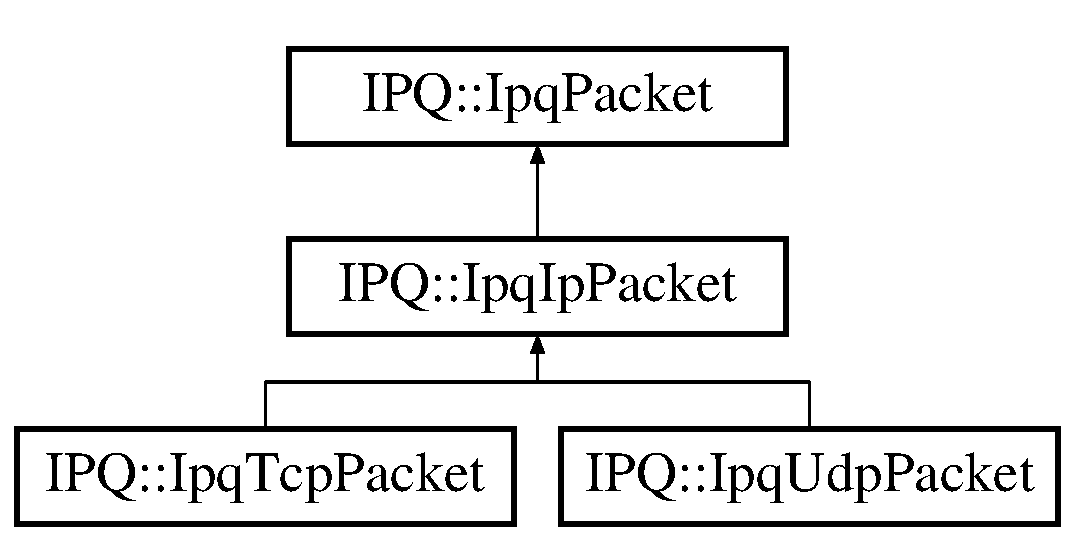
\includegraphics[height=3.000000cm]{classIPQ_1_1IpqPacket}
\end{center}
\end{figure}
\subsection*{\-Public \-Member \-Functions}
\begin{DoxyCompactItemize}
\item 
virtual \hyperlink{classIPQ_1_1IpqPacket_a2a0b25202791e9a0773b651b0c589626}{$\sim$\-Ipq\-Packet} ()
\begin{DoxyCompactList}\small\item\em \-Destructor for \hyperlink{classIPQ_1_1IpqPacket}{\-Ipq\-Packet}. \end{DoxyCompactList}\item 
unsigned long \hyperlink{classIPQ_1_1IpqPacket_ac3cbbe2b61e12730ffe231fa19c96e5a}{get\-Nf\-Id} () const 
\begin{DoxyCompactList}\small\item\em \-Retrieve the \-Netfilter \-I\-D of a packet. \end{DoxyCompactList}\item 
unsigned long \hyperlink{classIPQ_1_1IpqPacket_ab97f0a4348e53cb69ed1da74e422dc78}{get\-Nf\-Mark} () const 
\begin{DoxyCompactList}\small\item\em \-Retrieve the \-Netfilter mark value of a packet. \end{DoxyCompactList}\item 
void \hyperlink{classIPQ_1_1IpqPacket_a430ce4f89e651724efdf56c9c1b1647e}{get\-Timestamp} (struct timeval \&time) const 
\begin{DoxyCompactList}\small\item\em \-Retrieve the arrival time of a packet. \end{DoxyCompactList}\item 
unsigned \hyperlink{classIPQ_1_1IpqPacket_ae13884fedce165702f4b71e0e4d93c0b}{get\-Nf\-Hook} () const 
\begin{DoxyCompactList}\small\item\em \-Retrieve the number of the \-Netfilter hook on which the packet arrived. \end{DoxyCompactList}\item 
const char(\& \hyperlink{classIPQ_1_1IpqPacket_a4cf04ca5da28410f27d87edefd679532}{get\-Indev\-Name} () const)\mbox{[}\-I\-F\-N\-A\-M\-S\-I\-Z\mbox{]}
\begin{DoxyCompactList}\small\item\em \-Retrieve the name of the interface on which the packet arrived, if available. \end{DoxyCompactList}\item 
const char(\& \hyperlink{classIPQ_1_1IpqPacket_a46dced8057de3bba7abfaaa63d7afcd4}{get\-Outdev\-Name} () const)\mbox{[}\-I\-F\-N\-A\-M\-S\-I\-Z\mbox{]}
\begin{DoxyCompactList}\small\item\em \-Retrieve the name of the interface on which the packet will leave, if available. \end{DoxyCompactList}\item 
unsigned short \hyperlink{classIPQ_1_1IpqPacket_ae150e294f043f4c699231a85d3b1ae0f}{get\-Hw\-Protocol} () const 
\begin{DoxyCompactList}\small\item\em \-Retrieve the hardware protocol number of the packet. \end{DoxyCompactList}\item 
unsigned short \hyperlink{classIPQ_1_1IpqPacket_ab6b76b146111c7ad11b96e87efe6634c}{get\-Hw\-Type} () const 
\begin{DoxyCompactList}\small\item\em \-Retrieve the hardware type on which the packet arrived. \end{DoxyCompactList}\item 
const unsigned char(\& \hyperlink{classIPQ_1_1IpqPacket_a8582ae732d6b66ca1f5201994159a84a}{get\-Hw\-Source} (unsigned short \&addrlen) const)\mbox{[}8\mbox{]}
\begin{DoxyCompactList}\small\item\em \-Retrieve the source hardware address of the packet. \end{DoxyCompactList}\item 
const boost\-::uint8\-\_\-t $\ast$ \hyperlink{classIPQ_1_1IpqPacket_a6dd7baeec66082658d882bff8862eb6c}{get\-Packet} (std\-::size\-\_\-t \&size) const 
\begin{DoxyCompactList}\small\item\em \-Retrieve the packet. \end{DoxyCompactList}\item 
boost\-::uint8\-\_\-t $\ast$ \hyperlink{classIPQ_1_1IpqPacket_a0bf3344a9eed5e2f6bc20890ffffe26e}{get\-Packet} (std\-::size\-\_\-t \&size)
\begin{DoxyCompactList}\small\item\em \-Retrieve the packet. \end{DoxyCompactList}\item 
virtual void \hyperlink{classIPQ_1_1IpqPacket_a5fed4f899ba91b52d1734a083e67b3cf}{print} (std\-::ostream \&out) const 
\begin{DoxyCompactList}\small\item\em \-Print a packet to stdout in an easy-\/to-\/read format. \end{DoxyCompactList}\end{DoxyCompactItemize}
\subsection*{\-Protected \-Member \-Functions}
\begin{DoxyCompactItemize}
\item 
\hyperlink{classIPQ_1_1IpqPacket_a9ebf127442e021c3b25c8efa4711f531}{\-Ipq\-Packet} (\hyperlink{classLibWheel_1_1auto__array}{\-Lib\-Wheel\-::auto\-\_\-array}$<$ boost\-::uint8\-\_\-t $>$ buf, std\-::size\-\_\-t buflen)
\begin{DoxyCompactList}\small\item\em \-Constructor for \hyperlink{classIPQ_1_1IpqPacket}{\-Ipq\-Packet}. \end{DoxyCompactList}\item 
boost\-::uint8\-\_\-t $\ast$ \hyperlink{classIPQ_1_1IpqPacket_a7b8f489a9cec36058eaee43f6566a999}{do\-Get\-Packet} (std\-::size\-\_\-t \&size) const 
\begin{DoxyCompactList}\small\item\em \-Retrieve the packet. \end{DoxyCompactList}\item 
virtual void \hyperlink{classIPQ_1_1IpqPacket_a6e9ce8b7a24f8e82a82a7bc3859e9d45}{update\-Checksums} ()
\begin{DoxyCompactList}\small\item\em \-Update the packet's checksums and clear the dirty flag. \end{DoxyCompactList}\end{DoxyCompactItemize}
\subsection*{\-Static \-Protected \-Member \-Functions}
\begin{DoxyCompactItemize}
\item 
static \hyperlink{classIPQ_1_1IpqPacket}{\-Ipq\-Packet} $\ast$ \hyperlink{classIPQ_1_1IpqPacket_adf6099052730113814e9fe7312ec7b8c}{create\-Packet} (\hyperlink{classLibWheel_1_1auto__array}{\-Lib\-Wheel\-::auto\-\_\-array}$<$ boost\-::uint8\-\_\-t $>$ buf, std\-::size\-\_\-t buflen)
\begin{DoxyCompactList}\small\item\em \-Create an \hyperlink{classIPQ_1_1IpqPacket}{\-Ipq\-Packet} or one of its subclasses from a libipq packet message. \end{DoxyCompactList}\end{DoxyCompactItemize}
\subsection*{\-Protected \-Attributes}
\begin{DoxyCompactItemize}
\item 
\hyperlink{classLibWheel_1_1auto__array}{\-Lib\-Wheel\-::auto\-\_\-array}\*
$<$ boost\-::uint8\-\_\-t $>$ \hyperlink{classIPQ_1_1IpqPacket_a2bdf247f13a3e9f86e9e3846e6a9cb45}{packet}
\begin{DoxyCompactList}\small\item\em \-The packet message received from kernelspace. \end{DoxyCompactList}\item 
std\-::size\-\_\-t \hyperlink{classIPQ_1_1IpqPacket_a9b448a070c5ae499e32d2af5a190b86d}{packet\-Len}
\begin{DoxyCompactList}\small\item\em the length of the packet message in \hyperlink{classIPQ_1_1IpqPacket_a2bdf247f13a3e9f86e9e3846e6a9cb45}{\-Ipq\-Packet\-::packet}, in bytes. \end{DoxyCompactList}\item 
bool \hyperlink{classIPQ_1_1IpqPacket_a00acebf51531043a8536f20bb9412d61}{dirty}
\begin{DoxyCompactList}\small\item\em {\bfseries true} if the packet has been modified but checksums have not been updated; {\bfseries false} otherwise. \end{DoxyCompactList}\end{DoxyCompactItemize}
\subsection*{\-Private \-Attributes}
\begin{DoxyCompactItemize}
\item 
bool \hyperlink{classIPQ_1_1IpqPacket_aa1a2044e8f04423ccc68a4c0a2142c6b}{response\-Sent}
\begin{DoxyCompactList}\small\item\em {\bfseries true} if a verdict has been set on this packet; {\bfseries false} otherwise. \end{DoxyCompactList}\end{DoxyCompactItemize}
\subsection*{\-Friends}
\begin{DoxyCompactItemize}
\item 
\hyperlink{classIPQ_1_1IpqPacket}{\-Ipq\-Packet} $\ast$ \hyperlink{classIPQ_1_1IpqPacket_aadeb2b46a6c95963cc3edeb5638e360d}{\-Ipq\-Socket\-::recv\-Packet} (bool)
\begin{DoxyCompactList}\small\item\em \-Allow \hyperlink{classIPQ_1_1IpqSocket_aff35b95d33b21474f844660fef28938c}{\-Ipq\-Socket\-::recv\-Packet()} to access \hyperlink{classIPQ_1_1IpqPacket_adf6099052730113814e9fe7312ec7b8c}{create\-Packet()}. \end{DoxyCompactList}\item 
void \hyperlink{classIPQ_1_1IpqPacket_ac2316baee2ac9361e950dc6e059859aa}{\-Ipq\-Socket\-::send\-Response} (\hyperlink{classIPQ_1_1IpqPacket}{\-Ipq\-Packet} $\ast$, \-Verdict)
\begin{DoxyCompactList}\small\item\em \-Allow \hyperlink{classIPQ_1_1IpqSocket_a53e0f4e45363cbcd919a2d96ee7cf0a8}{\-Ipq\-Socket\-::send\-Response()} to access \hyperlink{classIPQ_1_1IpqPacket_aa1a2044e8f04423ccc68a4c0a2142c6b}{\-Ipq\-Packet\-::response\-Sent} and \hyperlink{classIPQ_1_1IpqPacket_a00acebf51531043a8536f20bb9412d61}{\-Ipq\-Packet\-::dirty}. \end{DoxyCompactList}\end{DoxyCompactItemize}


\subsection{\-Detailed \-Description}
\-Base class for packets received via \hyperlink{classIPQ_1_1IpqSocket}{\-Ipq\-Socket}. 

\-Contains all packet metadata fields, plus the original packet message from kernelspace.

\-A verdict must be set on each packet exactly once. \-When \hyperlink{classIPQ_1_1IpqSocket_a53e0f4e45363cbcd919a2d96ee7cf0a8}{\-Ipq\-Socket\-::send\-Response()} is used to set a verdict on a packet, the packet is flagged so that no new verdict can be set. \-If no verdict is set, the destructor to \hyperlink{classIPQ_1_1IpqPacket}{\-Ipq\-Packet} will set a verdict of \-D\-R\-O\-P.

\begin{DoxyNote}{\-Note}
\-Allowing copies of \-Ipq\-Packets to be made would break the response\-Sent checking. \-If it becomes necessary to make copies at some point, create an \-Ipq\-Packet\-Buffer class that contains all of the data and getters, but not response\-Set or the setters. \-Have \hyperlink{classIPQ_1_1IpqPacket}{\-Ipq\-Packet} inherit that, add the setters, give it a private copy constructor and assignment operator, and write an assignment operator that allows \-Ipq\-Packets to be safely assigned to \-Ipq\-Packet\-Buffers. \-The only way to create an \hyperlink{classIPQ_1_1IpqPacket}{\-Ipq\-Packet} should be from within \hyperlink{classIPQ_1_1IpqSocket_aff35b95d33b21474f844660fef28938c}{\-Ipq\-Socket\-::recv\-Packet()}. 
\end{DoxyNote}


\subsection{\-Constructor \& \-Destructor \-Documentation}
\hypertarget{classIPQ_1_1IpqPacket_a2a0b25202791e9a0773b651b0c589626}{
\index{\-I\-P\-Q\-::\-Ipq\-Packet@{\-I\-P\-Q\-::\-Ipq\-Packet}!$\sim$\-Ipq\-Packet@{$\sim$\-Ipq\-Packet}}
\index{$\sim$\-Ipq\-Packet@{$\sim$\-Ipq\-Packet}!IPQ::IpqPacket@{\-I\-P\-Q\-::\-Ipq\-Packet}}
\subsubsection[{$\sim$\-Ipq\-Packet}]{\setlength{\rightskip}{0pt plus 5cm}\-I\-P\-Q\-::\-Ipq\-Packet\-::$\sim$\-Ipq\-Packet (
\begin{DoxyParamCaption}
{}
\end{DoxyParamCaption}
)\hspace{0.3cm}{\ttfamily  \mbox{[}virtual\mbox{]}}}}
\label{classIPQ_1_1IpqPacket_a2a0b25202791e9a0773b651b0c589626}


\-Destructor for \hyperlink{classIPQ_1_1IpqPacket}{\-Ipq\-Packet}. 

\-If no response has been set for this packet, attempt to set a response of \-D\-R\-O\-P, and discard any exceptions thrown. 

\-Definition at line 500 of file \-I\-P\-Q.\-cpp.



\-References response\-Sent, \-I\-P\-Q\-::\-Ipq\-Socket\-::get\-Socket(), \-I\-P\-Q\-::\-Ipq\-Socket\-::send\-Response(), and \-I\-P\-Q\-::\-Ipq\-Socket\-::\-D\-R\-O\-P.

\hypertarget{classIPQ_1_1IpqPacket_a9ebf127442e021c3b25c8efa4711f531}{
\index{\-I\-P\-Q\-::\-Ipq\-Packet@{\-I\-P\-Q\-::\-Ipq\-Packet}!\-Ipq\-Packet@{\-Ipq\-Packet}}
\index{\-Ipq\-Packet@{\-Ipq\-Packet}!IPQ::IpqPacket@{\-I\-P\-Q\-::\-Ipq\-Packet}}
\subsubsection[{\-Ipq\-Packet}]{\setlength{\rightskip}{0pt plus 5cm}\-I\-P\-Q\-::\-Ipq\-Packet\-::\-Ipq\-Packet (
\begin{DoxyParamCaption}
\item[{{\bf \-Lib\-Wheel\-::auto\-\_\-array}$<$ boost\-::uint8\-\_\-t $>$}]{buf, }
\item[{std\-::size\-\_\-t}]{buflen}
\end{DoxyParamCaption}
)\hspace{0.3cm}{\ttfamily  \mbox{[}protected\mbox{]}}}}
\label{classIPQ_1_1IpqPacket_a9ebf127442e021c3b25c8efa4711f531}


\-Constructor for \hyperlink{classIPQ_1_1IpqPacket}{\-Ipq\-Packet}. 

\-Initialize an \hyperlink{classIPQ_1_1IpqPacket}{\-Ipq\-Packet} from a libipq packet message. 

\-Definition at line 685 of file \-I\-P\-Q.\-cpp.



\-Referenced by create\-Packet().



\subsection{\-Member \-Function \-Documentation}
\hypertarget{classIPQ_1_1IpqPacket_adf6099052730113814e9fe7312ec7b8c}{
\index{\-I\-P\-Q\-::\-Ipq\-Packet@{\-I\-P\-Q\-::\-Ipq\-Packet}!create\-Packet@{create\-Packet}}
\index{create\-Packet@{create\-Packet}!IPQ::IpqPacket@{\-I\-P\-Q\-::\-Ipq\-Packet}}
\subsubsection[{create\-Packet}]{\setlength{\rightskip}{0pt plus 5cm}{\bf \-Ipq\-Packet} $\ast$ \-I\-P\-Q\-::\-Ipq\-Packet\-::create\-Packet (
\begin{DoxyParamCaption}
\item[{{\bf \-Lib\-Wheel\-::auto\-\_\-array}$<$ boost\-::uint8\-\_\-t $>$}]{buf, }
\item[{std\-::size\-\_\-t}]{buflen}
\end{DoxyParamCaption}
)\hspace{0.3cm}{\ttfamily  \mbox{[}static, protected\mbox{]}}}}
\label{classIPQ_1_1IpqPacket_adf6099052730113814e9fe7312ec7b8c}


\-Create an \hyperlink{classIPQ_1_1IpqPacket}{\-Ipq\-Packet} or one of its subclasses from a libipq packet message. 

\-A packet will be deemed to be an \-I\-Pv4 packet if it has a full \-I\-Pv4 header and the data length indicated by the header matches the packet's length. \-A packet will be deemed to be a \-T\-C\-P or \-U\-D\-P packet if it is an \-I\-Pv4 packet and it has a full \-T\-C\-P or \-U\-D\-P header. \begin{DoxyReturn}{\-Returns}
\-A pointer to a dynamically-\/allocated \hyperlink{classIPQ_1_1IpqPacket}{\-Ipq\-Packet}, or one of its subclasses. \-This pointer must be freed using {\bfseries delete}, and a verdict should be set on it using \hyperlink{classIPQ_1_1IpqSocket_a53e0f4e45363cbcd919a2d96ee7cf0a8}{\-Ipq\-Socket\-::send\-Response()}. 
\end{DoxyReturn}


\-Definition at line 731 of file \-I\-P\-Q.\-cpp.



\-References \-Lib\-Wheel\-::auto\-\_\-array\-::get(), and \-Ipq\-Packet().



\-Referenced by \-I\-P\-Q\-::\-Ipq\-Socket\-::recv\-Packet().

\hypertarget{classIPQ_1_1IpqPacket_a7b8f489a9cec36058eaee43f6566a999}{
\index{\-I\-P\-Q\-::\-Ipq\-Packet@{\-I\-P\-Q\-::\-Ipq\-Packet}!do\-Get\-Packet@{do\-Get\-Packet}}
\index{do\-Get\-Packet@{do\-Get\-Packet}!IPQ::IpqPacket@{\-I\-P\-Q\-::\-Ipq\-Packet}}
\subsubsection[{do\-Get\-Packet}]{\setlength{\rightskip}{0pt plus 5cm}boost\-::uint8\-\_\-t $\ast$ \-I\-P\-Q\-::\-Ipq\-Packet\-::do\-Get\-Packet (
\begin{DoxyParamCaption}
\item[{std\-::size\-\_\-t \&}]{size}
\end{DoxyParamCaption}
) const\hspace{0.3cm}{\ttfamily  \mbox{[}protected\mbox{]}}}}
\label{classIPQ_1_1IpqPacket_a7b8f489a9cec36058eaee43f6566a999}


\-Retrieve the packet. 

\-It will only be available if the copy mode on the libipq handle used to receive it was \hyperlink{classIPQ_1_1IpqSocket_afee6d75480079906ecf6544f8467e0ccafc1e90369658a807b2c970d3e15b01d4}{\-Ipq\-Socket\-::\-P\-A\-C\-K\-E\-T} and the copy range was greater than zero. 
\begin{DoxyParams}[1]{\-Parameters}
\mbox{\tt out}  & {\em size} & \-A reference to a location to write the length of the payload, in bytes. \\
\hline
\end{DoxyParams}
\begin{DoxyReturn}{\-Returns}
\-A pointer to the packet. 
\end{DoxyReturn}


\-Definition at line 703 of file \-I\-P\-Q.\-cpp.



\-References packet, and \-Lib\-Wheel\-::auto\-\_\-array\-::get().



\-Referenced by get\-Packet().

\hypertarget{classIPQ_1_1IpqPacket_ae150e294f043f4c699231a85d3b1ae0f}{
\index{\-I\-P\-Q\-::\-Ipq\-Packet@{\-I\-P\-Q\-::\-Ipq\-Packet}!get\-Hw\-Protocol@{get\-Hw\-Protocol}}
\index{get\-Hw\-Protocol@{get\-Hw\-Protocol}!IPQ::IpqPacket@{\-I\-P\-Q\-::\-Ipq\-Packet}}
\subsubsection[{get\-Hw\-Protocol}]{\setlength{\rightskip}{0pt plus 5cm}unsigned short \-I\-P\-Q\-::\-Ipq\-Packet\-::get\-Hw\-Protocol (
\begin{DoxyParamCaption}
{}
\end{DoxyParamCaption}
) const}}
\label{classIPQ_1_1IpqPacket_ae150e294f043f4c699231a85d3b1ae0f}


\-Retrieve the hardware protocol number of the packet. 

\begin{DoxyReturn}{\-Returns}
\-The packet's hardware protocol number. 
\end{DoxyReturn}


\-Definition at line 585 of file \-I\-P\-Q.\-cpp.



\-References packet, and \-Lib\-Wheel\-::auto\-\_\-array\-::get().



\-Referenced by print().

\hypertarget{classIPQ_1_1IpqPacket_a8582ae732d6b66ca1f5201994159a84a}{
\index{\-I\-P\-Q\-::\-Ipq\-Packet@{\-I\-P\-Q\-::\-Ipq\-Packet}!get\-Hw\-Source@{get\-Hw\-Source}}
\index{get\-Hw\-Source@{get\-Hw\-Source}!IPQ::IpqPacket@{\-I\-P\-Q\-::\-Ipq\-Packet}}
\subsubsection[{get\-Hw\-Source}]{\setlength{\rightskip}{0pt plus 5cm}const unsigned char(\& \-I\-P\-Q\-::\-Ipq\-Packet\-::get\-Hw\-Source (
\begin{DoxyParamCaption}
\item[{unsigned short \&}]{addrlen}
\end{DoxyParamCaption}
))\mbox{[}8\mbox{]}}}
\label{classIPQ_1_1IpqPacket_a8582ae732d6b66ca1f5201994159a84a}


\-Retrieve the source hardware address of the packet. 


\begin{DoxyParams}[1]{\-Parameters}
\mbox{\tt out}  & {\em addrlen} & \-A reference to a location to write the actual length of the address, in bytes. \\
\hline
\end{DoxyParams}
\begin{DoxyReturn}{\-Returns}
\-A reference to the packet's source hardware address. 
\end{DoxyReturn}


\-Definition at line 608 of file \-I\-P\-Q.\-cpp.



\-Referenced by print().

\hypertarget{classIPQ_1_1IpqPacket_ab6b76b146111c7ad11b96e87efe6634c}{
\index{\-I\-P\-Q\-::\-Ipq\-Packet@{\-I\-P\-Q\-::\-Ipq\-Packet}!get\-Hw\-Type@{get\-Hw\-Type}}
\index{get\-Hw\-Type@{get\-Hw\-Type}!IPQ::IpqPacket@{\-I\-P\-Q\-::\-Ipq\-Packet}}
\subsubsection[{get\-Hw\-Type}]{\setlength{\rightskip}{0pt plus 5cm}unsigned short \-I\-P\-Q\-::\-Ipq\-Packet\-::get\-Hw\-Type (
\begin{DoxyParamCaption}
{}
\end{DoxyParamCaption}
) const}}
\label{classIPQ_1_1IpqPacket_ab6b76b146111c7ad11b96e87efe6634c}


\-Retrieve the hardware type on which the packet arrived. 

\begin{DoxyReturn}{\-Returns}
\-The packet's arrival hardware type. 
\end{DoxyReturn}


\-Definition at line 596 of file \-I\-P\-Q.\-cpp.



\-References packet, and \-Lib\-Wheel\-::auto\-\_\-array\-::get().



\-Referenced by print().

\hypertarget{classIPQ_1_1IpqPacket_a4cf04ca5da28410f27d87edefd679532}{
\index{\-I\-P\-Q\-::\-Ipq\-Packet@{\-I\-P\-Q\-::\-Ipq\-Packet}!get\-Indev\-Name@{get\-Indev\-Name}}
\index{get\-Indev\-Name@{get\-Indev\-Name}!IPQ::IpqPacket@{\-I\-P\-Q\-::\-Ipq\-Packet}}
\subsubsection[{get\-Indev\-Name}]{\setlength{\rightskip}{0pt plus 5cm}const char(\& \-I\-P\-Q\-::\-Ipq\-Packet\-::get\-Indev\-Name (
\begin{DoxyParamCaption}
{}
\end{DoxyParamCaption}
))\mbox{[}\-I\-F\-N\-A\-M\-S\-I\-Z\mbox{]}}}
\label{classIPQ_1_1IpqPacket_a4cf04ca5da28410f27d87edefd679532}


\-Retrieve the name of the interface on which the packet arrived, if available. 

\begin{DoxyReturn}{\-Returns}
\-A reference to the packet's arrival interface name. 
\end{DoxyReturn}


\-Definition at line 563 of file \-I\-P\-Q.\-cpp.



\-Referenced by print().

\hypertarget{classIPQ_1_1IpqPacket_ae13884fedce165702f4b71e0e4d93c0b}{
\index{\-I\-P\-Q\-::\-Ipq\-Packet@{\-I\-P\-Q\-::\-Ipq\-Packet}!get\-Nf\-Hook@{get\-Nf\-Hook}}
\index{get\-Nf\-Hook@{get\-Nf\-Hook}!IPQ::IpqPacket@{\-I\-P\-Q\-::\-Ipq\-Packet}}
\subsubsection[{get\-Nf\-Hook}]{\setlength{\rightskip}{0pt plus 5cm}unsigned \-I\-P\-Q\-::\-Ipq\-Packet\-::get\-Nf\-Hook (
\begin{DoxyParamCaption}
{}
\end{DoxyParamCaption}
) const}}
\label{classIPQ_1_1IpqPacket_ae13884fedce165702f4b71e0e4d93c0b}


\-Retrieve the number of the \-Netfilter hook on which the packet arrived. 

\begin{DoxyReturn}{\-Returns}
\-The number of the \-Netfilter hook on which the packet arrived. 
\end{DoxyReturn}


\-Definition at line 553 of file \-I\-P\-Q.\-cpp.



\-References packet, and \-Lib\-Wheel\-::auto\-\_\-array\-::get().



\-Referenced by print().

\hypertarget{classIPQ_1_1IpqPacket_ac3cbbe2b61e12730ffe231fa19c96e5a}{
\index{\-I\-P\-Q\-::\-Ipq\-Packet@{\-I\-P\-Q\-::\-Ipq\-Packet}!get\-Nf\-Id@{get\-Nf\-Id}}
\index{get\-Nf\-Id@{get\-Nf\-Id}!IPQ::IpqPacket@{\-I\-P\-Q\-::\-Ipq\-Packet}}
\subsubsection[{get\-Nf\-Id}]{\setlength{\rightskip}{0pt plus 5cm}unsigned long \-I\-P\-Q\-::\-Ipq\-Packet\-::get\-Nf\-Id (
\begin{DoxyParamCaption}
{}
\end{DoxyParamCaption}
) const}}
\label{classIPQ_1_1IpqPacket_ac3cbbe2b61e12730ffe231fa19c96e5a}


\-Retrieve the \-Netfilter \-I\-D of a packet. 

\begin{DoxyReturn}{\-Returns}
\-The packet's \-Netfilter \-I\-D. 
\end{DoxyReturn}


\-Definition at line 519 of file \-I\-P\-Q.\-cpp.



\-References packet, and \-Lib\-Wheel\-::auto\-\_\-array\-::get().



\-Referenced by \-I\-P\-Q\-::\-Ipq\-Socket\-::recv\-Packet(), and print().

\hypertarget{classIPQ_1_1IpqPacket_ab97f0a4348e53cb69ed1da74e422dc78}{
\index{\-I\-P\-Q\-::\-Ipq\-Packet@{\-I\-P\-Q\-::\-Ipq\-Packet}!get\-Nf\-Mark@{get\-Nf\-Mark}}
\index{get\-Nf\-Mark@{get\-Nf\-Mark}!IPQ::IpqPacket@{\-I\-P\-Q\-::\-Ipq\-Packet}}
\subsubsection[{get\-Nf\-Mark}]{\setlength{\rightskip}{0pt plus 5cm}unsigned long \-I\-P\-Q\-::\-Ipq\-Packet\-::get\-Nf\-Mark (
\begin{DoxyParamCaption}
{}
\end{DoxyParamCaption}
) const}}
\label{classIPQ_1_1IpqPacket_ab97f0a4348e53cb69ed1da74e422dc78}


\-Retrieve the \-Netfilter mark value of a packet. 

\begin{DoxyReturn}{\-Returns}
\-The packet's \-Netfilter mark value. 
\end{DoxyReturn}


\-Definition at line 530 of file \-I\-P\-Q.\-cpp.



\-References packet, and \-Lib\-Wheel\-::auto\-\_\-array\-::get().



\-Referenced by print().

\hypertarget{classIPQ_1_1IpqPacket_a46dced8057de3bba7abfaaa63d7afcd4}{
\index{\-I\-P\-Q\-::\-Ipq\-Packet@{\-I\-P\-Q\-::\-Ipq\-Packet}!get\-Outdev\-Name@{get\-Outdev\-Name}}
\index{get\-Outdev\-Name@{get\-Outdev\-Name}!IPQ::IpqPacket@{\-I\-P\-Q\-::\-Ipq\-Packet}}
\subsubsection[{get\-Outdev\-Name}]{\setlength{\rightskip}{0pt plus 5cm}const char(\& \-I\-P\-Q\-::\-Ipq\-Packet\-::get\-Outdev\-Name (
\begin{DoxyParamCaption}
{}
\end{DoxyParamCaption}
))\mbox{[}\-I\-F\-N\-A\-M\-S\-I\-Z\mbox{]}}}
\label{classIPQ_1_1IpqPacket_a46dced8057de3bba7abfaaa63d7afcd4}


\-Retrieve the name of the interface on which the packet will leave, if available. 

\begin{DoxyReturn}{\-Returns}
\-A reference to the packet's outbound interface name. 
\end{DoxyReturn}


\-Definition at line 574 of file \-I\-P\-Q.\-cpp.



\-Referenced by print().

\hypertarget{classIPQ_1_1IpqPacket_a6dd7baeec66082658d882bff8862eb6c}{
\index{\-I\-P\-Q\-::\-Ipq\-Packet@{\-I\-P\-Q\-::\-Ipq\-Packet}!get\-Packet@{get\-Packet}}
\index{get\-Packet@{get\-Packet}!IPQ::IpqPacket@{\-I\-P\-Q\-::\-Ipq\-Packet}}
\subsubsection[{get\-Packet}]{\setlength{\rightskip}{0pt plus 5cm}const boost\-::uint8\-\_\-t $\ast$ \-I\-P\-Q\-::\-Ipq\-Packet\-::get\-Packet (
\begin{DoxyParamCaption}
\item[{std\-::size\-\_\-t \&}]{size}
\end{DoxyParamCaption}
) const}}
\label{classIPQ_1_1IpqPacket_a6dd7baeec66082658d882bff8862eb6c}


\-Retrieve the packet. 

\-It will only be available if the copy mode on the libipq handle used to receive it was \hyperlink{classIPQ_1_1IpqSocket_afee6d75480079906ecf6544f8467e0ccafc1e90369658a807b2c970d3e15b01d4}{\-Ipq\-Socket\-::\-P\-A\-C\-K\-E\-T} and the copy range was greater than zero. 
\begin{DoxyParams}[1]{\-Parameters}
\mbox{\tt out}  & {\em size} & \-A reference to a location to write the length of the payload, in bytes. \\
\hline
\end{DoxyParams}
\begin{DoxyReturn}{\-Returns}
\-A const pointer to the packet. 
\end{DoxyReturn}


\-Definition at line 624 of file \-I\-P\-Q.\-cpp.



\-References do\-Get\-Packet().



\-Referenced by \-I\-P\-Q\-::\-Ipq\-Socket\-::recv\-Packet().

\hypertarget{classIPQ_1_1IpqPacket_a0bf3344a9eed5e2f6bc20890ffffe26e}{
\index{\-I\-P\-Q\-::\-Ipq\-Packet@{\-I\-P\-Q\-::\-Ipq\-Packet}!get\-Packet@{get\-Packet}}
\index{get\-Packet@{get\-Packet}!IPQ::IpqPacket@{\-I\-P\-Q\-::\-Ipq\-Packet}}
\subsubsection[{get\-Packet}]{\setlength{\rightskip}{0pt plus 5cm}boost\-::uint8\-\_\-t $\ast$ \-I\-P\-Q\-::\-Ipq\-Packet\-::get\-Packet (
\begin{DoxyParamCaption}
\item[{std\-::size\-\_\-t \&}]{size}
\end{DoxyParamCaption}
)}}
\label{classIPQ_1_1IpqPacket_a0bf3344a9eed5e2f6bc20890ffffe26e}


\-Retrieve the packet. 

\-It will only be available if the copy mode on the libipq handle used to receive it was \hyperlink{classIPQ_1_1IpqSocket_afee6d75480079906ecf6544f8467e0ccafc1e90369658a807b2c970d3e15b01d4}{\-Ipq\-Socket\-::\-P\-A\-C\-K\-E\-T} and the copy range was greater than zero. 
\begin{DoxyParams}[1]{\-Parameters}
\mbox{\tt out}  & {\em size} & \-A reference to a location to write the length of the payload, in bytes. \\
\hline
\end{DoxyParams}
\begin{DoxyReturn}{\-Returns}
\-A pointer to the packet. 
\end{DoxyReturn}
\begin{DoxyNote}{\-Note}
\-This method sets the packet's dirty flag, requiring that the packet's checksums be recomputed before a verdict is set. 
\end{DoxyNote}


\-Definition at line 641 of file \-I\-P\-Q.\-cpp.



\-References dirty, and do\-Get\-Packet().

\hypertarget{classIPQ_1_1IpqPacket_a430ce4f89e651724efdf56c9c1b1647e}{
\index{\-I\-P\-Q\-::\-Ipq\-Packet@{\-I\-P\-Q\-::\-Ipq\-Packet}!get\-Timestamp@{get\-Timestamp}}
\index{get\-Timestamp@{get\-Timestamp}!IPQ::IpqPacket@{\-I\-P\-Q\-::\-Ipq\-Packet}}
\subsubsection[{get\-Timestamp}]{\setlength{\rightskip}{0pt plus 5cm}void \-I\-P\-Q\-::\-Ipq\-Packet\-::get\-Timestamp (
\begin{DoxyParamCaption}
\item[{struct timeval \&}]{time}
\end{DoxyParamCaption}
) const}}
\label{classIPQ_1_1IpqPacket_a430ce4f89e651724efdf56c9c1b1647e}


\-Retrieve the arrival time of a packet. 

\begin{DoxyReturn}{\-Returns}
\-The packet's arrival time. 
\end{DoxyReturn}


\-Definition at line 541 of file \-I\-P\-Q.\-cpp.



\-References packet, and \-Lib\-Wheel\-::auto\-\_\-array\-::get().



\-Referenced by print().

\hypertarget{classIPQ_1_1IpqPacket_a5fed4f899ba91b52d1734a083e67b3cf}{
\index{\-I\-P\-Q\-::\-Ipq\-Packet@{\-I\-P\-Q\-::\-Ipq\-Packet}!print@{print}}
\index{print@{print}!IPQ::IpqPacket@{\-I\-P\-Q\-::\-Ipq\-Packet}}
\subsubsection[{print}]{\setlength{\rightskip}{0pt plus 5cm}void \-I\-P\-Q\-::\-Ipq\-Packet\-::print (
\begin{DoxyParamCaption}
\item[{std\-::ostream \&}]{out}
\end{DoxyParamCaption}
) const\hspace{0.3cm}{\ttfamily  \mbox{[}virtual\mbox{]}}}}
\label{classIPQ_1_1IpqPacket_a5fed4f899ba91b52d1734a083e67b3cf}


\-Print a packet to stdout in an easy-\/to-\/read format. 



\-Reimplemented in \hyperlink{classIPQ_1_1IpqUdpPacket_ad64646eb338bad97b6c593ad5225d36d}{\-I\-P\-Q\-::\-Ipq\-Udp\-Packet}, \hyperlink{classIPQ_1_1IpqTcpPacket_a751f98aa2aafbe6796bf3a82d7273bec}{\-I\-P\-Q\-::\-Ipq\-Tcp\-Packet}, and \hyperlink{classIPQ_1_1IpqIpPacket_a5ddc175ec8c4bc8c7bab3baee12909f0}{\-I\-P\-Q\-::\-Ipq\-Ip\-Packet}.



\-Definition at line 652 of file \-I\-P\-Q.\-cpp.



\-References get\-Timestamp(), get\-Hw\-Source(), get\-Nf\-Id(), get\-Nf\-Mark(), get\-Nf\-Hook(), get\-Indev\-Name(), get\-Outdev\-Name(), get\-Hw\-Protocol(), get\-Hw\-Type(), packet, and \-Lib\-Wheel\-::auto\-\_\-array\-::get().

\hypertarget{classIPQ_1_1IpqPacket_a6e9ce8b7a24f8e82a82a7bc3859e9d45}{
\index{\-I\-P\-Q\-::\-Ipq\-Packet@{\-I\-P\-Q\-::\-Ipq\-Packet}!update\-Checksums@{update\-Checksums}}
\index{update\-Checksums@{update\-Checksums}!IPQ::IpqPacket@{\-I\-P\-Q\-::\-Ipq\-Packet}}
\subsubsection[{update\-Checksums}]{\setlength{\rightskip}{0pt plus 5cm}void \-I\-P\-Q\-::\-Ipq\-Packet\-::update\-Checksums (
\begin{DoxyParamCaption}
{}
\end{DoxyParamCaption}
)\hspace{0.3cm}{\ttfamily  \mbox{[}protected, virtual\mbox{]}}}}
\label{classIPQ_1_1IpqPacket_a6e9ce8b7a24f8e82a82a7bc3859e9d45}


\-Update the packet's checksums and clear the dirty flag. 



\-Reimplemented in \hyperlink{classIPQ_1_1IpqUdpPacket_abc390e2f22ffbd3d6d9a2df228cb71d6}{\-I\-P\-Q\-::\-Ipq\-Udp\-Packet}, \hyperlink{classIPQ_1_1IpqTcpPacket_aa3c42606d262b29f2b4bef459f34dd90}{\-I\-P\-Q\-::\-Ipq\-Tcp\-Packet}, and \hyperlink{classIPQ_1_1IpqIpPacket_a4c2c0ccd36ef921f6632b26ebd524b90}{\-I\-P\-Q\-::\-Ipq\-Ip\-Packet}.



\-Definition at line 714 of file \-I\-P\-Q.\-cpp.



\-References dirty.



\subsection{\-Friends \-And \-Related \-Function \-Documentation}
\hypertarget{classIPQ_1_1IpqPacket_aadeb2b46a6c95963cc3edeb5638e360d}{
\index{\-I\-P\-Q\-::\-Ipq\-Packet@{\-I\-P\-Q\-::\-Ipq\-Packet}!\-Ipq\-Socket\-::recv\-Packet@{\-Ipq\-Socket\-::recv\-Packet}}
\index{\-Ipq\-Socket\-::recv\-Packet@{\-Ipq\-Socket\-::recv\-Packet}!IPQ::IpqPacket@{\-I\-P\-Q\-::\-Ipq\-Packet}}
\subsubsection[{\-Ipq\-Socket\-::recv\-Packet}]{\setlength{\rightskip}{0pt plus 5cm}{\bf \-Ipq\-Packet}$\ast$ \-Ipq\-Socket\-::recv\-Packet (
\begin{DoxyParamCaption}
\item[{bool}]{}
\end{DoxyParamCaption}
)\hspace{0.3cm}{\ttfamily  \mbox{[}friend\mbox{]}}}}
\label{classIPQ_1_1IpqPacket_aadeb2b46a6c95963cc3edeb5638e360d}


\-Allow \hyperlink{classIPQ_1_1IpqSocket_aff35b95d33b21474f844660fef28938c}{\-Ipq\-Socket\-::recv\-Packet()} to access \hyperlink{classIPQ_1_1IpqPacket_adf6099052730113814e9fe7312ec7b8c}{create\-Packet()}. 

\hypertarget{classIPQ_1_1IpqPacket_ac2316baee2ac9361e950dc6e059859aa}{
\index{\-I\-P\-Q\-::\-Ipq\-Packet@{\-I\-P\-Q\-::\-Ipq\-Packet}!\-Ipq\-Socket\-::send\-Response@{\-Ipq\-Socket\-::send\-Response}}
\index{\-Ipq\-Socket\-::send\-Response@{\-Ipq\-Socket\-::send\-Response}!IPQ::IpqPacket@{\-I\-P\-Q\-::\-Ipq\-Packet}}
\subsubsection[{\-Ipq\-Socket\-::send\-Response}]{\setlength{\rightskip}{0pt plus 5cm}void \-Ipq\-Socket\-::send\-Response (
\begin{DoxyParamCaption}
\item[{{\bf \-Ipq\-Packet} $\ast$}]{, }
\item[{\-Verdict}]{}
\end{DoxyParamCaption}
)\hspace{0.3cm}{\ttfamily  \mbox{[}friend\mbox{]}}}}
\label{classIPQ_1_1IpqPacket_ac2316baee2ac9361e950dc6e059859aa}


\-Allow \hyperlink{classIPQ_1_1IpqSocket_a53e0f4e45363cbcd919a2d96ee7cf0a8}{\-Ipq\-Socket\-::send\-Response()} to access \hyperlink{classIPQ_1_1IpqPacket_aa1a2044e8f04423ccc68a4c0a2142c6b}{\-Ipq\-Packet\-::response\-Sent} and \hyperlink{classIPQ_1_1IpqPacket_a00acebf51531043a8536f20bb9412d61}{\-Ipq\-Packet\-::dirty}. 



\subsection{\-Member \-Data \-Documentation}
\hypertarget{classIPQ_1_1IpqPacket_a00acebf51531043a8536f20bb9412d61}{
\index{\-I\-P\-Q\-::\-Ipq\-Packet@{\-I\-P\-Q\-::\-Ipq\-Packet}!dirty@{dirty}}
\index{dirty@{dirty}!IPQ::IpqPacket@{\-I\-P\-Q\-::\-Ipq\-Packet}}
\subsubsection[{dirty}]{\setlength{\rightskip}{0pt plus 5cm}bool {\bf \-I\-P\-Q\-::\-Ipq\-Packet\-::dirty}\hspace{0.3cm}{\ttfamily  \mbox{[}protected\mbox{]}}}}
\label{classIPQ_1_1IpqPacket_a00acebf51531043a8536f20bb9412d61}


{\bfseries true} if the packet has been modified but checksums have not been updated; {\bfseries false} otherwise. 



\-Definition at line 171 of file \-I\-P\-Q.\-hpp.



\-Referenced by get\-Packet(), update\-Checksums(), \-I\-P\-Q\-::\-Ipq\-Ip\-Packet\-::get\-Ip\-Header(), \-I\-P\-Q\-::\-Ipq\-Ip\-Packet\-::get\-Ip\-Payload(), \-I\-P\-Q\-::\-Ipq\-Tcp\-Packet\-::get\-Tcp\-Header(), \-I\-P\-Q\-::\-Ipq\-Tcp\-Packet\-::get\-Tcp\-Payload(), \-I\-P\-Q\-::\-Ipq\-Udp\-Packet\-::get\-Udp\-Header(), and \-I\-P\-Q\-::\-Ipq\-Udp\-Packet\-::get\-Udp\-Payload().

\hypertarget{classIPQ_1_1IpqPacket_a2bdf247f13a3e9f86e9e3846e6a9cb45}{
\index{\-I\-P\-Q\-::\-Ipq\-Packet@{\-I\-P\-Q\-::\-Ipq\-Packet}!packet@{packet}}
\index{packet@{packet}!IPQ::IpqPacket@{\-I\-P\-Q\-::\-Ipq\-Packet}}
\subsubsection[{packet}]{\setlength{\rightskip}{0pt plus 5cm}{\bf \-Lib\-Wheel\-::auto\-\_\-array}$<$boost\-::uint8\-\_\-t$>$ {\bf \-I\-P\-Q\-::\-Ipq\-Packet\-::packet}\hspace{0.3cm}{\ttfamily  \mbox{[}protected\mbox{]}}}}
\label{classIPQ_1_1IpqPacket_a2bdf247f13a3e9f86e9e3846e6a9cb45}


\-The packet message received from kernelspace. 



\-Definition at line 169 of file \-I\-P\-Q.\-hpp.



\-Referenced by get\-Nf\-Id(), get\-Nf\-Mark(), get\-Timestamp(), get\-Nf\-Hook(), get\-Hw\-Protocol(), get\-Hw\-Type(), print(), do\-Get\-Packet(), \-I\-P\-Q\-::\-Ipq\-Ip\-Packet\-::do\-Get\-Ip\-Header(), \-I\-P\-Q\-::\-Ipq\-Ip\-Packet\-::do\-Get\-Ip\-Payload(), \-I\-P\-Q\-::\-Ipq\-Tcp\-Packet\-::do\-Get\-Tcp\-Header(), \-I\-P\-Q\-::\-Ipq\-Tcp\-Packet\-::do\-Get\-Tcp\-Payload(), \-I\-P\-Q\-::\-Ipq\-Tcp\-Packet\-::update\-Checksums(), \-I\-P\-Q\-::\-Ipq\-Udp\-Packet\-::do\-Get\-Udp\-Header(), \-I\-P\-Q\-::\-Ipq\-Udp\-Packet\-::do\-Get\-Udp\-Payload(), and \-I\-P\-Q\-::\-Ipq\-Udp\-Packet\-::update\-Checksums().

\hypertarget{classIPQ_1_1IpqPacket_a9b448a070c5ae499e32d2af5a190b86d}{
\index{\-I\-P\-Q\-::\-Ipq\-Packet@{\-I\-P\-Q\-::\-Ipq\-Packet}!packet\-Len@{packet\-Len}}
\index{packet\-Len@{packet\-Len}!IPQ::IpqPacket@{\-I\-P\-Q\-::\-Ipq\-Packet}}
\subsubsection[{packet\-Len}]{\setlength{\rightskip}{0pt plus 5cm}std\-::size\-\_\-t {\bf \-I\-P\-Q\-::\-Ipq\-Packet\-::packet\-Len}\hspace{0.3cm}{\ttfamily  \mbox{[}protected\mbox{]}}}}
\label{classIPQ_1_1IpqPacket_a9b448a070c5ae499e32d2af5a190b86d}


the length of the packet message in \hyperlink{classIPQ_1_1IpqPacket_a2bdf247f13a3e9f86e9e3846e6a9cb45}{\-Ipq\-Packet\-::packet}, in bytes. 



\-Definition at line 170 of file \-I\-P\-Q.\-hpp.

\hypertarget{classIPQ_1_1IpqPacket_aa1a2044e8f04423ccc68a4c0a2142c6b}{
\index{\-I\-P\-Q\-::\-Ipq\-Packet@{\-I\-P\-Q\-::\-Ipq\-Packet}!response\-Sent@{response\-Sent}}
\index{response\-Sent@{response\-Sent}!IPQ::IpqPacket@{\-I\-P\-Q\-::\-Ipq\-Packet}}
\subsubsection[{response\-Sent}]{\setlength{\rightskip}{0pt plus 5cm}bool {\bf \-I\-P\-Q\-::\-Ipq\-Packet\-::response\-Sent}\hspace{0.3cm}{\ttfamily  \mbox{[}private\mbox{]}}}}
\label{classIPQ_1_1IpqPacket_aa1a2044e8f04423ccc68a4c0a2142c6b}


{\bfseries true} if a verdict has been set on this packet; {\bfseries false} otherwise. 



\-Definition at line 179 of file \-I\-P\-Q.\-hpp.



\-Referenced by $\sim$\-Ipq\-Packet().



\-The documentation for this class was generated from the following files\-:\begin{DoxyCompactItemize}
\item 
\hyperlink{IPQ_8hpp}{\-I\-P\-Q.\-hpp}\item 
\hyperlink{IPQ_8cpp}{\-I\-P\-Q.\-cpp}\end{DoxyCompactItemize}

\hypertarget{classIPQ_1_1IpqSocket}{
\section{\-I\-P\-Q\-:\-:\-Ipq\-Socket \-Class \-Reference}
\label{classIPQ_1_1IpqSocket}\index{\-I\-P\-Q\-::\-Ipq\-Socket@{\-I\-P\-Q\-::\-Ipq\-Socket}}
}


\-A program's link to libipq.  




{\ttfamily \#include $<$\-I\-P\-Q.\-hpp$>$}

\subsection*{\-Public \-Types}
\begin{DoxyCompactItemize}
\item 
enum \hyperlink{classIPQ_1_1IpqSocket_afee6d75480079906ecf6544f8467e0cc}{\-Copy\-Mode} \{ \hyperlink{classIPQ_1_1IpqSocket_afee6d75480079906ecf6544f8467e0cca68b0f4a778230f9a60087417daa76310}{\-M\-E\-T\-A}, 
\hyperlink{classIPQ_1_1IpqSocket_afee6d75480079906ecf6544f8467e0ccafc1e90369658a807b2c970d3e15b01d4}{\-P\-A\-C\-K\-E\-T}
 \}
\begin{DoxyCompactList}\small\item\em \-The amount of packet information to copy to userspace. \end{DoxyCompactList}\item 
enum \hyperlink{classIPQ_1_1IpqSocket_a2aaaf01ab3bdb3a4a7f90dd142fd93cc}{\-Verdict} \{ \hyperlink{classIPQ_1_1IpqSocket_a2aaaf01ab3bdb3a4a7f90dd142fd93cca2f14f71dc344cea511b9a9e7a553ed99}{\-A\-C\-C\-E\-P\-T}, 
\hyperlink{classIPQ_1_1IpqSocket_a2aaaf01ab3bdb3a4a7f90dd142fd93cca95ff3c260279df28c833d51ffa1b8c46}{\-D\-R\-O\-P}, 
\hyperlink{classIPQ_1_1IpqSocket_a2aaaf01ab3bdb3a4a7f90dd142fd93cca2de248ccae41d7a288cda6a629ecdcf5}{\-S\-T\-O\-P}
 \}
\begin{DoxyCompactList}\small\item\em \-The verdict to set on a packet. \end{DoxyCompactList}\end{DoxyCompactItemize}
\subsection*{\-Public \-Member \-Functions}
\begin{DoxyCompactItemize}
\item 
void \hyperlink{classIPQ_1_1IpqSocket_aaf97b48f357008b4858605d94a37cd1e}{connect} ()  throw (\-Ipq\-Exception)
\begin{DoxyCompactList}\small\item\em \-Connect to libipq. \end{DoxyCompactList}\item 
void \hyperlink{classIPQ_1_1IpqSocket_abec3b30403b9763467cb66cd5e8bbfe4}{set\-Copy\-Mode} (\hyperlink{classIPQ_1_1IpqSocket_afee6d75480079906ecf6544f8467e0cc}{\-Copy\-Mode} mode, std\-::size\-\_\-t range=65535)  throw (\-Ipq\-Exception)
\begin{DoxyCompactList}\small\item\em \-Sets the libipq copy mode. \end{DoxyCompactList}\item 
\hyperlink{classIPQ_1_1IpqPacket}{\-Ipq\-Packet} $\ast$ \hyperlink{classIPQ_1_1IpqSocket_aff35b95d33b21474f844660fef28938c}{recv\-Packet} (bool noblock=false)  throw (\-Ipq\-Exception)
\begin{DoxyCompactList}\small\item\em \-Receive a packet from libipq. \end{DoxyCompactList}\item 
void \hyperlink{classIPQ_1_1IpqSocket_a123e77a47324d0c765e191153659c040}{wait\-For\-Packet} ()  throw (\-Ipq\-Exception)
\begin{DoxyCompactList}\small\item\em \-Wait for a packet to become available. \end{DoxyCompactList}\item 
void \hyperlink{classIPQ_1_1IpqSocket_a32af8892fbf20202f4265a771d06bb3a}{wait\-For\-Packet} (int func\-\_\-fd, boost\-::function$<$ void()$>$ func)
\begin{DoxyCompactList}\small\item\em \-Wait for a packet to become available. \end{DoxyCompactList}\item 
void \hyperlink{classIPQ_1_1IpqSocket_a53e0f4e45363cbcd919a2d96ee7cf0a8}{send\-Response} (\hyperlink{classIPQ_1_1IpqPacket}{\-Ipq\-Packet} $\ast$pkt, \hyperlink{classIPQ_1_1IpqSocket_a2aaaf01ab3bdb3a4a7f90dd142fd93cc}{\-Verdict} v)  throw (\-Ipq\-Exception)
\begin{DoxyCompactList}\small\item\em \-Sets the verdict on a packet. \end{DoxyCompactList}\item 
void \hyperlink{classIPQ_1_1IpqSocket_a9a6fe5c8f61ae31fc59771f07fa37007}{close} ()  throw (\-Ipq\-Exception)
\begin{DoxyCompactList}\small\item\em \-Close the libipq handle. \end{DoxyCompactList}\item 
unsigned long \hyperlink{classIPQ_1_1IpqSocket_a9e664c8e6a5a549feb27d3052e7ff28b}{get\-Packets\-Received} () const 
\begin{DoxyCompactList}\small\item\em \-Retrieve the number of packets that have been received from libipq. \end{DoxyCompactList}\item 
unsigned long \hyperlink{classIPQ_1_1IpqSocket_a83b3c143170568625923218daf2c6864}{get\-Packets\-Accepted} () const 
\begin{DoxyCompactList}\small\item\em \-Retrieve the number of packets for which a verdict of \-A\-C\-C\-E\-P\-T or \-S\-T\-O\-P was set. \end{DoxyCompactList}\item 
unsigned long \hyperlink{classIPQ_1_1IpqSocket_a902f0bc0d1106b6da00ca4ce18a65ffa}{get\-Packets\-Dropped} () const 
\begin{DoxyCompactList}\small\item\em \-Retrieve the number of packets for which a verdict of \-D\-R\-O\-P was set. \end{DoxyCompactList}\end{DoxyCompactItemize}
\subsection*{\-Static \-Public \-Member \-Functions}
\begin{DoxyCompactItemize}
\item 
static \hyperlink{classIPQ_1_1IpqSocket}{\-Ipq\-Socket} \& \hyperlink{classIPQ_1_1IpqSocket_a036ccfa7bf9f4c81e74e3d52362ba9e8}{get\-Socket} ()
\begin{DoxyCompactList}\small\item\em \-Retrieve the global libipq handle. \end{DoxyCompactList}\end{DoxyCompactItemize}
\subsection*{\-Protected \-Member \-Functions}
\begin{DoxyCompactItemize}
\item 
\hyperlink{classIPQ_1_1IpqSocket_a1fb5a8dbb5d40703b1c43c68dc370c36}{\-Ipq\-Socket} ()
\begin{DoxyCompactList}\small\item\em \-Constructor for \hyperlink{classIPQ_1_1IpqSocket}{\-Ipq\-Socket}. \end{DoxyCompactList}\item 
\hyperlink{classIPQ_1_1IpqSocket_ada019c192f17b98ffa34f8eafc64e500}{$\sim$\-Ipq\-Socket} ()
\begin{DoxyCompactList}\small\item\em \-Destructor for \hyperlink{classIPQ_1_1IpqSocket}{\-Ipq\-Socket}. \end{DoxyCompactList}\end{DoxyCompactItemize}
\subsection*{\-Private \-Attributes}
\begin{DoxyCompactItemize}
\item 
bool \hyperlink{classIPQ_1_1IpqSocket_a5f17c2492bd9205c4120e8dbeec652d2}{is\-Connected}
\begin{DoxyCompactList}\small\item\em {\bfseries true} on sockets that are connected; {\bfseries false} otherwise. \end{DoxyCompactList}\item 
\hyperlink{classIPQ_1_1IpqSocket_afee6d75480079906ecf6544f8467e0cc}{\-Copy\-Mode} \hyperlink{classIPQ_1_1IpqSocket_adef58e75a6d67b6179ff73b59ff49eeb}{copy\-Mode}
\begin{DoxyCompactList}\small\item\em \-The amount of packet data to copy from kernelspace. \end{DoxyCompactList}\item 
struct ipq\-\_\-handle $\ast$ \hyperlink{classIPQ_1_1IpqSocket_ad4d1b18fe03e035fb76f6bcd6eaa32cb}{ipq\-Handle}
\begin{DoxyCompactList}\small\item\em \-Handle to libipq. \end{DoxyCompactList}\item 
unsigned long \hyperlink{classIPQ_1_1IpqSocket_a85d2411c577e4bec30b15d3ec43a21f0}{packets\-Received}
\begin{DoxyCompactList}\small\item\em \-The number of packets that have been received. \end{DoxyCompactList}\item 
unsigned long \hyperlink{classIPQ_1_1IpqSocket_a50304942c2b695fecdb496d6d424937a}{packets\-Accepted}
\begin{DoxyCompactList}\small\item\em \-The number of packets for which \-A\-C\-C\-E\-P\-T or \-S\-T\-O\-P verdicts have been set. \end{DoxyCompactList}\item 
unsigned long \hyperlink{classIPQ_1_1IpqSocket_acc24abac49471076d9555f58afb0d162}{packets\-Dropped}
\begin{DoxyCompactList}\small\item\em \-The number of packets for which \-D\-R\-O\-P verdicts have been set. \end{DoxyCompactList}\end{DoxyCompactItemize}


\subsection{\-Detailed \-Description}
\-A program's link to libipq. 

\-Only one program can use libipq at a time. \begin{DoxyWarning}{\-Warning}
\-This class is not thread-\/safe. 
\end{DoxyWarning}
\begin{DoxyRefDesc}{\-Bug}
\item[\hyperlink{bug__bug000001}{\-Bug}]\-Connect() does not detect if other another program is using libipq. \-Instead, if another program is connected, \hyperlink{classIPQ_1_1IpqSocket_aff35b95d33b21474f844660fef28938c}{recv\-Packet()} will throw an exception. \-This is due to a limitation in libipq. 

\-Due to a bug in \-Netfilter, changing the source \-I\-P address of a packet to a non-\/local address and then setting a verdict of \-N\-F\-\_\-\-A\-C\-C\-E\-P\-T will cause it to be dropped. \-This has been observed when the packet was queued from the \-O\-U\-T\-P\-U\-T chain of the mangle table. \-A work-\/around is to set a verdict of \-N\-F\-\_\-\-S\-T\-O\-P instead of \-N\-F\-\_\-\-A\-C\-C\-E\-P\-T, but be aware that this results in the packet being treated differently by iptables. \-Kernels prior to 2.\-6.\-12 do not have \-N\-F\-\_\-\-S\-T\-O\-P; defining \-N\-O\-\_\-\-N\-F\-\_\-\-S\-T\-O\-P enables another work-\/around\-: all packets are immediately dropped, and packets that are to be accepted are re-\/injected through raw sockets. \-In this case, care must be taken to ensure that infinite queueing loops do not occur. \-Also, this work-\/around only works for \-I\-P packets. \end{DoxyRefDesc}


\subsection{\-Member \-Enumeration \-Documentation}
\hypertarget{classIPQ_1_1IpqSocket_afee6d75480079906ecf6544f8467e0cc}{
\index{\-I\-P\-Q\-::\-Ipq\-Socket@{\-I\-P\-Q\-::\-Ipq\-Socket}!\-Copy\-Mode@{\-Copy\-Mode}}
\index{\-Copy\-Mode@{\-Copy\-Mode}!IPQ::IpqSocket@{\-I\-P\-Q\-::\-Ipq\-Socket}}
\subsubsection[{\-Copy\-Mode}]{\setlength{\rightskip}{0pt plus 5cm}enum {\bf \-I\-P\-Q\-::\-Ipq\-Socket\-::\-Copy\-Mode}}}
\label{classIPQ_1_1IpqSocket_afee6d75480079906ecf6544f8467e0cc}


\-The amount of packet information to copy to userspace. 

\begin{Desc}
\item[\-Enumerator\-: ]\par
\begin{description}
\index{\-M\-E\-T\-A@{\-M\-E\-T\-A}!\-I\-P\-Q\-::\-Ipq\-Socket@{\-I\-P\-Q\-::\-Ipq\-Socket}}\index{\-I\-P\-Q\-::\-Ipq\-Socket@{\-I\-P\-Q\-::\-Ipq\-Socket}!\-M\-E\-T\-A@{\-M\-E\-T\-A}}\item[{\em 
\hypertarget{classIPQ_1_1IpqSocket_afee6d75480079906ecf6544f8467e0cca68b0f4a778230f9a60087417daa76310}{
\-M\-E\-T\-A}
\label{classIPQ_1_1IpqSocket_afee6d75480079906ecf6544f8467e0cca68b0f4a778230f9a60087417daa76310}
}]\-Copy packet medatada only. \index{\-P\-A\-C\-K\-E\-T@{\-P\-A\-C\-K\-E\-T}!\-I\-P\-Q\-::\-Ipq\-Socket@{\-I\-P\-Q\-::\-Ipq\-Socket}}\index{\-I\-P\-Q\-::\-Ipq\-Socket@{\-I\-P\-Q\-::\-Ipq\-Socket}!\-P\-A\-C\-K\-E\-T@{\-P\-A\-C\-K\-E\-T}}\item[{\em 
\hypertarget{classIPQ_1_1IpqSocket_afee6d75480079906ecf6544f8467e0ccafc1e90369658a807b2c970d3e15b01d4}{
\-P\-A\-C\-K\-E\-T}
\label{classIPQ_1_1IpqSocket_afee6d75480079906ecf6544f8467e0ccafc1e90369658a807b2c970d3e15b01d4}
}]\-Copy both packet metadata and contents. \end{description}
\end{Desc}



\-Definition at line 85 of file \-I\-P\-Q.\-hpp.

\hypertarget{classIPQ_1_1IpqSocket_a2aaaf01ab3bdb3a4a7f90dd142fd93cc}{
\index{\-I\-P\-Q\-::\-Ipq\-Socket@{\-I\-P\-Q\-::\-Ipq\-Socket}!\-Verdict@{\-Verdict}}
\index{\-Verdict@{\-Verdict}!IPQ::IpqSocket@{\-I\-P\-Q\-::\-Ipq\-Socket}}
\subsubsection[{\-Verdict}]{\setlength{\rightskip}{0pt plus 5cm}enum {\bf \-I\-P\-Q\-::\-Ipq\-Socket\-::\-Verdict}}}
\label{classIPQ_1_1IpqSocket_a2aaaf01ab3bdb3a4a7f90dd142fd93cc}


\-The verdict to set on a packet. 

\begin{Desc}
\item[\-Enumerator\-: ]\par
\begin{description}
\index{\-A\-C\-C\-E\-P\-T@{\-A\-C\-C\-E\-P\-T}!\-I\-P\-Q\-::\-Ipq\-Socket@{\-I\-P\-Q\-::\-Ipq\-Socket}}\index{\-I\-P\-Q\-::\-Ipq\-Socket@{\-I\-P\-Q\-::\-Ipq\-Socket}!\-A\-C\-C\-E\-P\-T@{\-A\-C\-C\-E\-P\-T}}\item[{\em 
\hypertarget{classIPQ_1_1IpqSocket_a2aaaf01ab3bdb3a4a7f90dd142fd93cca2f14f71dc344cea511b9a9e7a553ed99}{
\-A\-C\-C\-E\-P\-T}
\label{classIPQ_1_1IpqSocket_a2aaaf01ab3bdb3a4a7f90dd142fd93cca2f14f71dc344cea511b9a9e7a553ed99}
}]\-Accept the packet and continue iptables traversal. \index{\-D\-R\-O\-P@{\-D\-R\-O\-P}!\-I\-P\-Q\-::\-Ipq\-Socket@{\-I\-P\-Q\-::\-Ipq\-Socket}}\index{\-I\-P\-Q\-::\-Ipq\-Socket@{\-I\-P\-Q\-::\-Ipq\-Socket}!\-D\-R\-O\-P@{\-D\-R\-O\-P}}\item[{\em 
\hypertarget{classIPQ_1_1IpqSocket_a2aaaf01ab3bdb3a4a7f90dd142fd93cca95ff3c260279df28c833d51ffa1b8c46}{
\-D\-R\-O\-P}
\label{classIPQ_1_1IpqSocket_a2aaaf01ab3bdb3a4a7f90dd142fd93cca95ff3c260279df28c833d51ffa1b8c46}
}]\-Drop the packet. \index{\-S\-T\-O\-P@{\-S\-T\-O\-P}!\-I\-P\-Q\-::\-Ipq\-Socket@{\-I\-P\-Q\-::\-Ipq\-Socket}}\index{\-I\-P\-Q\-::\-Ipq\-Socket@{\-I\-P\-Q\-::\-Ipq\-Socket}!\-S\-T\-O\-P@{\-S\-T\-O\-P}}\item[{\em 
\hypertarget{classIPQ_1_1IpqSocket_a2aaaf01ab3bdb3a4a7f90dd142fd93cca2de248ccae41d7a288cda6a629ecdcf5}{
\-S\-T\-O\-P}
\label{classIPQ_1_1IpqSocket_a2aaaf01ab3bdb3a4a7f90dd142fd93cca2de248ccae41d7a288cda6a629ecdcf5}
}]\-Accept the packet, but don't continue iptables traversal. \end{description}
\end{Desc}



\-Definition at line 90 of file \-I\-P\-Q.\-hpp.



\subsection{\-Constructor \& \-Destructor \-Documentation}
\hypertarget{classIPQ_1_1IpqSocket_a1fb5a8dbb5d40703b1c43c68dc370c36}{
\index{\-I\-P\-Q\-::\-Ipq\-Socket@{\-I\-P\-Q\-::\-Ipq\-Socket}!\-Ipq\-Socket@{\-Ipq\-Socket}}
\index{\-Ipq\-Socket@{\-Ipq\-Socket}!IPQ::IpqSocket@{\-I\-P\-Q\-::\-Ipq\-Socket}}
\subsubsection[{\-Ipq\-Socket}]{\setlength{\rightskip}{0pt plus 5cm}\-I\-P\-Q\-::\-Ipq\-Socket\-::\-Ipq\-Socket (
\begin{DoxyParamCaption}
{}
\end{DoxyParamCaption}
)\hspace{0.3cm}{\ttfamily  \mbox{[}protected\mbox{]}}}}
\label{classIPQ_1_1IpqSocket_a1fb5a8dbb5d40703b1c43c68dc370c36}


\-Constructor for \hyperlink{classIPQ_1_1IpqSocket}{\-Ipq\-Socket}. 

\-Initialize an unconnected libipq handle. 

\-Definition at line 453 of file \-I\-P\-Q.\-cpp.

\hypertarget{classIPQ_1_1IpqSocket_ada019c192f17b98ffa34f8eafc64e500}{
\index{\-I\-P\-Q\-::\-Ipq\-Socket@{\-I\-P\-Q\-::\-Ipq\-Socket}!$\sim$\-Ipq\-Socket@{$\sim$\-Ipq\-Socket}}
\index{$\sim$\-Ipq\-Socket@{$\sim$\-Ipq\-Socket}!IPQ::IpqSocket@{\-I\-P\-Q\-::\-Ipq\-Socket}}
\subsubsection[{$\sim$\-Ipq\-Socket}]{\setlength{\rightskip}{0pt plus 5cm}\-I\-P\-Q\-::\-Ipq\-Socket\-::$\sim$\-Ipq\-Socket (
\begin{DoxyParamCaption}
{}
\end{DoxyParamCaption}
)\hspace{0.3cm}{\ttfamily  \mbox{[}protected\mbox{]}}}}
\label{classIPQ_1_1IpqSocket_ada019c192f17b98ffa34f8eafc64e500}


\-Destructor for \hyperlink{classIPQ_1_1IpqSocket}{\-Ipq\-Socket}. 

\-If the handle is open, close it and discard any exceptions thrown. 

\-Definition at line 468 of file \-I\-P\-Q.\-cpp.



\-References close().



\subsection{\-Member \-Function \-Documentation}
\hypertarget{classIPQ_1_1IpqSocket_a9a6fe5c8f61ae31fc59771f07fa37007}{
\index{\-I\-P\-Q\-::\-Ipq\-Socket@{\-I\-P\-Q\-::\-Ipq\-Socket}!close@{close}}
\index{close@{close}!IPQ::IpqSocket@{\-I\-P\-Q\-::\-Ipq\-Socket}}
\subsubsection[{close}]{\setlength{\rightskip}{0pt plus 5cm}void \-I\-P\-Q\-::\-Ipq\-Socket\-::close (
\begin{DoxyParamCaption}
{}
\end{DoxyParamCaption}
)  throw ({\bf \-Ipq\-Exception})}}
\label{classIPQ_1_1IpqSocket_a9a6fe5c8f61ae31fc59771f07fa37007}


\-Close the libipq handle. 

\-If the handle is not open, no action is taken. 
\begin{DoxyExceptions}{\-Exceptions}
{\em \hyperlink{classIPQ_1_1IpqException}{\-Ipq\-Exception}} & \-If an error was encountered closing the handle. \\
\hline
\end{DoxyExceptions}
\begin{DoxyWarning}{\-Warning}
\-Do not close the handle without ensuring that verdicts have been set on all packets received. \-Since the destructor to \hyperlink{classIPQ_1_1IpqPacket}{\-Ipq\-Packet} attempts to set a verdict on unresponded packets, \-Bad \-Things (tm) will happen if the handle is closed. 
\end{DoxyWarning}


\-Definition at line 243 of file \-I\-P\-Q.\-cpp.



\-References is\-Connected, and ipq\-Handle.



\-Referenced by $\sim$\-Ipq\-Socket(), and \-N\-E\-R\-D\-::\-Connection\-Server\-::$\sim$\-Connection\-Server().

\hypertarget{classIPQ_1_1IpqSocket_aaf97b48f357008b4858605d94a37cd1e}{
\index{\-I\-P\-Q\-::\-Ipq\-Socket@{\-I\-P\-Q\-::\-Ipq\-Socket}!connect@{connect}}
\index{connect@{connect}!IPQ::IpqSocket@{\-I\-P\-Q\-::\-Ipq\-Socket}}
\subsubsection[{connect}]{\setlength{\rightskip}{0pt plus 5cm}void \-I\-P\-Q\-::\-Ipq\-Socket\-::connect (
\begin{DoxyParamCaption}
{}
\end{DoxyParamCaption}
)  throw ({\bf \-Ipq\-Exception})}}
\label{classIPQ_1_1IpqSocket_aaf97b48f357008b4858605d94a37cd1e}


\-Connect to libipq. 

\-Sets the default copy mode to metadata only. \-If \-N\-O\-\_\-\-N\-F\-\_\-\-S\-T\-O\-P is defined, open raw\-\_\-sock as well. 
\begin{DoxyExceptions}{\-Exceptions}
{\em \hyperlink{classIPQ_1_1IpqException}{\-Ipq\-Exception}} & \-If the socket is already connected or there is an error connecting. \\
\hline
\end{DoxyExceptions}


\-Definition at line 113 of file \-I\-P\-Q.\-cpp.



\-References is\-Connected, ipq\-Handle, set\-Copy\-Mode(), and \-M\-E\-T\-A.

\hypertarget{classIPQ_1_1IpqSocket_a83b3c143170568625923218daf2c6864}{
\index{\-I\-P\-Q\-::\-Ipq\-Socket@{\-I\-P\-Q\-::\-Ipq\-Socket}!get\-Packets\-Accepted@{get\-Packets\-Accepted}}
\index{get\-Packets\-Accepted@{get\-Packets\-Accepted}!IPQ::IpqSocket@{\-I\-P\-Q\-::\-Ipq\-Socket}}
\subsubsection[{get\-Packets\-Accepted}]{\setlength{\rightskip}{0pt plus 5cm}unsigned long \-I\-P\-Q\-::\-Ipq\-Socket\-::get\-Packets\-Accepted (
\begin{DoxyParamCaption}
{}
\end{DoxyParamCaption}
) const}}
\label{classIPQ_1_1IpqSocket_a83b3c143170568625923218daf2c6864}


\-Retrieve the number of packets for which a verdict of \-A\-C\-C\-E\-P\-T or \-S\-T\-O\-P was set. 

\begin{DoxyReturn}{\-Returns}
\-The number of packets accepted. 
\end{DoxyReturn}


\-Definition at line 432 of file \-I\-P\-Q.\-cpp.



\-References packets\-Accepted.



\-Referenced by \-N\-E\-R\-D\-::\-Connection\-Server\-::print\-Stats().

\hypertarget{classIPQ_1_1IpqSocket_a902f0bc0d1106b6da00ca4ce18a65ffa}{
\index{\-I\-P\-Q\-::\-Ipq\-Socket@{\-I\-P\-Q\-::\-Ipq\-Socket}!get\-Packets\-Dropped@{get\-Packets\-Dropped}}
\index{get\-Packets\-Dropped@{get\-Packets\-Dropped}!IPQ::IpqSocket@{\-I\-P\-Q\-::\-Ipq\-Socket}}
\subsubsection[{get\-Packets\-Dropped}]{\setlength{\rightskip}{0pt plus 5cm}unsigned long \-I\-P\-Q\-::\-Ipq\-Socket\-::get\-Packets\-Dropped (
\begin{DoxyParamCaption}
{}
\end{DoxyParamCaption}
) const}}
\label{classIPQ_1_1IpqSocket_a902f0bc0d1106b6da00ca4ce18a65ffa}


\-Retrieve the number of packets for which a verdict of \-D\-R\-O\-P was set. 

\begin{DoxyReturn}{\-Returns}
\-The number of packets dropped. 
\end{DoxyReturn}


\-Definition at line 443 of file \-I\-P\-Q.\-cpp.



\-References packets\-Dropped.



\-Referenced by \-N\-E\-R\-D\-::\-Connection\-Server\-::print\-Stats().

\hypertarget{classIPQ_1_1IpqSocket_a9e664c8e6a5a549feb27d3052e7ff28b}{
\index{\-I\-P\-Q\-::\-Ipq\-Socket@{\-I\-P\-Q\-::\-Ipq\-Socket}!get\-Packets\-Received@{get\-Packets\-Received}}
\index{get\-Packets\-Received@{get\-Packets\-Received}!IPQ::IpqSocket@{\-I\-P\-Q\-::\-Ipq\-Socket}}
\subsubsection[{get\-Packets\-Received}]{\setlength{\rightskip}{0pt plus 5cm}unsigned long \-I\-P\-Q\-::\-Ipq\-Socket\-::get\-Packets\-Received (
\begin{DoxyParamCaption}
{}
\end{DoxyParamCaption}
) const}}
\label{classIPQ_1_1IpqSocket_a9e664c8e6a5a549feb27d3052e7ff28b}


\-Retrieve the number of packets that have been received from libipq. 

\begin{DoxyReturn}{\-Returns}
\-The number of packets received. 
\end{DoxyReturn}


\-Definition at line 421 of file \-I\-P\-Q.\-cpp.



\-References packets\-Received.



\-Referenced by \-N\-E\-R\-D\-::\-Connection\-Server\-::print\-Stats().

\hypertarget{classIPQ_1_1IpqSocket_a036ccfa7bf9f4c81e74e3d52362ba9e8}{
\index{\-I\-P\-Q\-::\-Ipq\-Socket@{\-I\-P\-Q\-::\-Ipq\-Socket}!get\-Socket@{get\-Socket}}
\index{get\-Socket@{get\-Socket}!IPQ::IpqSocket@{\-I\-P\-Q\-::\-Ipq\-Socket}}
\subsubsection[{get\-Socket}]{\setlength{\rightskip}{0pt plus 5cm}{\bf \-Ipq\-Socket} \& \-I\-P\-Q\-::\-Ipq\-Socket\-::get\-Socket (
\begin{DoxyParamCaption}
{}
\end{DoxyParamCaption}
)\hspace{0.3cm}{\ttfamily  \mbox{[}static\mbox{]}}}}
\label{classIPQ_1_1IpqSocket_a036ccfa7bf9f4c81e74e3d52362ba9e8}


\-Retrieve the global libipq handle. 

\begin{DoxyReturn}{\-Returns}
\-A reference to the global libipq handle. 
\end{DoxyReturn}


\-Definition at line 99 of file \-I\-P\-Q.\-cpp.



\-Referenced by \-I\-P\-Q\-::\-Ipq\-Packet\-::$\sim$\-Ipq\-Packet().

\hypertarget{classIPQ_1_1IpqSocket_aff35b95d33b21474f844660fef28938c}{
\index{\-I\-P\-Q\-::\-Ipq\-Socket@{\-I\-P\-Q\-::\-Ipq\-Socket}!recv\-Packet@{recv\-Packet}}
\index{recv\-Packet@{recv\-Packet}!IPQ::IpqSocket@{\-I\-P\-Q\-::\-Ipq\-Socket}}
\subsubsection[{recv\-Packet}]{\setlength{\rightskip}{0pt plus 5cm}{\bf \-Ipq\-Packet} $\ast$ \-I\-P\-Q\-::\-Ipq\-Socket\-::recv\-Packet (
\begin{DoxyParamCaption}
\item[{bool}]{noblock = {\ttfamily false}}
\end{DoxyParamCaption}
)  throw ({\bf \-Ipq\-Exception})}}
\label{classIPQ_1_1IpqSocket_aff35b95d33b21474f844660fef28938c}


\-Receive a packet from libipq. 


\begin{DoxyParams}{\-Parameters}
{\em noblock} & \-If {\bfseries true}, throw an \hyperlink{classIPQ_1_1IpqException}{\-Ipq\-Exception} if no packet is available. \-If {\bfseries false}, block until a packet becomes available. (default\-: {\bfseries false}) \\
\hline
\end{DoxyParams}
\begin{DoxyReturn}{\-Returns}
\-A dynamically-\/allocated packet object, which may be an \hyperlink{classIPQ_1_1IpqPacket}{\-Ipq\-Packet} or any of its subclasses. \-It must be freed using {\bfseries delete}, and a verdict {\itshape should\/} be set on it using \hyperlink{classIPQ_1_1IpqSocket_a53e0f4e45363cbcd919a2d96ee7cf0a8}{\-Ipq\-Socket\-::send\-Response()}. 
\end{DoxyReturn}

\begin{DoxyExceptions}{\-Exceptions}
{\em \hyperlink{classIPQ_1_1IpqException}{\-Ipq\-Exception}} & \-If there was an error reading from the socket, no packet was immediately available and {\itshape noblock\/} was set, or a libipq error message was received. \\
\hline
\end{DoxyExceptions}
\begin{DoxyNote}{\-Note}
\-If {\itshape noblock\/} was not set, then this method may block indefinately. 

\-If \-N\-O\-\_\-\-N\-F\-\_\-\-S\-T\-O\-P is defined, the packet is immediately dropped. \-It may be re-\/injected using \hyperlink{classIPQ_1_1IpqSocket_a53e0f4e45363cbcd919a2d96ee7cf0a8}{\-Ipq\-Socket\-::send\-Response()}. 
\end{DoxyNote}


\-Definition at line 277 of file \-I\-P\-Q.\-cpp.



\-References \-Lib\-Wheel\-::auto\-\_\-array\-::get(), \-I\-P\-Q\-::\-Ipq\-Packet\-::create\-Packet(), \-I\-P\-Q\-::\-Ipq\-Packet\-::get\-Packet(), and \-I\-P\-Q\-::\-Ipq\-Packet\-::get\-Nf\-Id().



\-Referenced by \-N\-E\-R\-D\-::\-Connection\-Server\-::operator()().

\hypertarget{classIPQ_1_1IpqSocket_a53e0f4e45363cbcd919a2d96ee7cf0a8}{
\index{\-I\-P\-Q\-::\-Ipq\-Socket@{\-I\-P\-Q\-::\-Ipq\-Socket}!send\-Response@{send\-Response}}
\index{send\-Response@{send\-Response}!IPQ::IpqSocket@{\-I\-P\-Q\-::\-Ipq\-Socket}}
\subsubsection[{send\-Response}]{\setlength{\rightskip}{0pt plus 5cm}void \-I\-P\-Q\-::\-Ipq\-Socket\-::send\-Response (
\begin{DoxyParamCaption}
\item[{{\bf \-Ipq\-Packet} $\ast$}]{pkt, }
\item[{{\bf \-Verdict}}]{v}
\end{DoxyParamCaption}
)  throw ({\bf \-Ipq\-Exception})}}
\label{classIPQ_1_1IpqSocket_a53e0f4e45363cbcd919a2d96ee7cf0a8}


\-Sets the verdict on a packet. 

\-If the packet was changed, the original packet will be replaced with the modified version. \-If a verdict was already set on {\itshape pkt\/}, no action is taken beyond updating the packet checksums. 
\begin{DoxyParams}{\-Parameters}
{\em pkt} & \-The packet whose verdict to set. \\
\hline
{\em v} & \-The verdict to set. \\
\hline
\end{DoxyParams}

\begin{DoxyExceptions}{\-Exceptions}
{\em \hyperlink{classIPQ_1_1IpqException}{\-Ipq\-Exception}} & \-If the verdict is invalid or there was an error setting the verdict. \\
\hline
\end{DoxyExceptions}
\begin{DoxyNote}{\-Note}
\-If \-N\-O\-\_\-\-N\-F\-\_\-\-S\-T\-O\-P is set, a verdict cannot be safely set, so a copy of the packet in injected through a raw socket. \-Care must be taken to avoid infinite loops. 
\end{DoxyNote}


\-Definition at line 177 of file \-I\-P\-Q.\-cpp.



\-References \-N\-F\-\_\-\-S\-T\-O\-P, \-Lib\-Wheel\-::array\-Size(), and \-I\-P\-Q\-::\-Ipq\-Ip\-Packet\-::get\-Ip\-Dest().



\-Referenced by \-I\-P\-Q\-::\-Ipq\-Packet\-::$\sim$\-Ipq\-Packet(), \-N\-E\-R\-D\-::\-Connection\-Server\-::\-Server\-Writeback\-Handler\-::operator()(), \-N\-E\-R\-D\-::\-Connection\-Server\-::handle\-Packet(), and \-N\-E\-R\-D\-::\-Connection\-Server\-::create\-Connection().

\hypertarget{classIPQ_1_1IpqSocket_abec3b30403b9763467cb66cd5e8bbfe4}{
\index{\-I\-P\-Q\-::\-Ipq\-Socket@{\-I\-P\-Q\-::\-Ipq\-Socket}!set\-Copy\-Mode@{set\-Copy\-Mode}}
\index{set\-Copy\-Mode@{set\-Copy\-Mode}!IPQ::IpqSocket@{\-I\-P\-Q\-::\-Ipq\-Socket}}
\subsubsection[{set\-Copy\-Mode}]{\setlength{\rightskip}{0pt plus 5cm}void \-I\-P\-Q\-::\-Ipq\-Socket\-::set\-Copy\-Mode (
\begin{DoxyParamCaption}
\item[{{\bf \-Copy\-Mode}}]{mode, }
\item[{std\-::size\-\_\-t}]{range = {\ttfamily 65535}}
\end{DoxyParamCaption}
)  throw ({\bf \-Ipq\-Exception})}}
\label{classIPQ_1_1IpqSocket_abec3b30403b9763467cb66cd5e8bbfe4}


\-Sets the libipq copy mode. 


\begin{DoxyParams}{\-Parameters}
{\em mode} & \-The libipq copy mode. \\
\hline
{\em range} & \-The number of packet payload bytes to copy (default\-: 65535). \-This is only used if {\itshape mode\/} is \-P\-A\-C\-K\-E\-T. \\
\hline
\end{DoxyParams}

\begin{DoxyExceptions}{\-Exceptions}
{\em \hyperlink{classIPQ_1_1IpqException}{\-Ipq\-Exception}} & if the socket is not connected, the mode is invalid, or there is an error setting the mode. \\
\hline
\end{DoxyExceptions}


\-Definition at line 145 of file \-I\-P\-Q.\-cpp.



\-References \-Lib\-Wheel\-::array\-Size().



\-Referenced by connect().

\hypertarget{classIPQ_1_1IpqSocket_a123e77a47324d0c765e191153659c040}{
\index{\-I\-P\-Q\-::\-Ipq\-Socket@{\-I\-P\-Q\-::\-Ipq\-Socket}!wait\-For\-Packet@{wait\-For\-Packet}}
\index{wait\-For\-Packet@{wait\-For\-Packet}!IPQ::IpqSocket@{\-I\-P\-Q\-::\-Ipq\-Socket}}
\subsubsection[{wait\-For\-Packet}]{\setlength{\rightskip}{0pt plus 5cm}void \-I\-P\-Q\-::\-Ipq\-Socket\-::wait\-For\-Packet (
\begin{DoxyParamCaption}
{}
\end{DoxyParamCaption}
)  throw ({\bf \-Ipq\-Exception})}}
\label{classIPQ_1_1IpqSocket_a123e77a47324d0c765e191153659c040}


\-Wait for a packet to become available. 


\begin{DoxyExceptions}{\-Exceptions}
{\em \hyperlink{classIPQ_1_1IpqException}{\-Ipq\-Exception}} & \-If an error was encountered checking for a packet. \\
\hline
\end{DoxyExceptions}
\begin{DoxyNote}{\-Note}
\-This method may block indefinately. 
\end{DoxyNote}


\-Definition at line 362 of file \-I\-P\-Q.\-cpp.



\-References ipq\-Handle.



\-Referenced by \-N\-E\-R\-D\-::\-Connection\-Server\-::operator()().

\hypertarget{classIPQ_1_1IpqSocket_a32af8892fbf20202f4265a771d06bb3a}{
\index{\-I\-P\-Q\-::\-Ipq\-Socket@{\-I\-P\-Q\-::\-Ipq\-Socket}!wait\-For\-Packet@{wait\-For\-Packet}}
\index{wait\-For\-Packet@{wait\-For\-Packet}!IPQ::IpqSocket@{\-I\-P\-Q\-::\-Ipq\-Socket}}
\subsubsection[{wait\-For\-Packet}]{\setlength{\rightskip}{0pt plus 5cm}void \-I\-P\-Q\-::\-Ipq\-Socket\-::wait\-For\-Packet (
\begin{DoxyParamCaption}
\item[{int}]{func\-\_\-fd, }
\item[{boost\-::function$<$ void()$>$}]{func}
\end{DoxyParamCaption}
)}}
\label{classIPQ_1_1IpqSocket_a32af8892fbf20202f4265a771d06bb3a}


\-Wait for a packet to become available. 

\-If input becomes available on {\itshape func\-\_\-fd\/} before a packet arrives, call {\itshape func\/}, and resume waiting. \begin{DoxyNote}{\-Note}
\-This method may block indefinately. 
\end{DoxyNote}


\-Definition at line 384 of file \-I\-P\-Q.\-cpp.



\-References ipq\-Handle.



\subsection{\-Member \-Data \-Documentation}
\hypertarget{classIPQ_1_1IpqSocket_adef58e75a6d67b6179ff73b59ff49eeb}{
\index{\-I\-P\-Q\-::\-Ipq\-Socket@{\-I\-P\-Q\-::\-Ipq\-Socket}!copy\-Mode@{copy\-Mode}}
\index{copy\-Mode@{copy\-Mode}!IPQ::IpqSocket@{\-I\-P\-Q\-::\-Ipq\-Socket}}
\subsubsection[{copy\-Mode}]{\setlength{\rightskip}{0pt plus 5cm}{\bf \-Copy\-Mode} {\bf \-I\-P\-Q\-::\-Ipq\-Socket\-::copy\-Mode}\hspace{0.3cm}{\ttfamily  \mbox{[}private\mbox{]}}}}
\label{classIPQ_1_1IpqSocket_adef58e75a6d67b6179ff73b59ff49eeb}


\-The amount of packet data to copy from kernelspace. 



\-Definition at line 114 of file \-I\-P\-Q.\-hpp.

\hypertarget{classIPQ_1_1IpqSocket_ad4d1b18fe03e035fb76f6bcd6eaa32cb}{
\index{\-I\-P\-Q\-::\-Ipq\-Socket@{\-I\-P\-Q\-::\-Ipq\-Socket}!ipq\-Handle@{ipq\-Handle}}
\index{ipq\-Handle@{ipq\-Handle}!IPQ::IpqSocket@{\-I\-P\-Q\-::\-Ipq\-Socket}}
\subsubsection[{ipq\-Handle}]{\setlength{\rightskip}{0pt plus 5cm}struct ipq\-\_\-handle$\ast$ {\bf \-I\-P\-Q\-::\-Ipq\-Socket\-::ipq\-Handle}\hspace{0.3cm}{\ttfamily  \mbox{[}private\mbox{]}}}}
\label{classIPQ_1_1IpqSocket_ad4d1b18fe03e035fb76f6bcd6eaa32cb}


\-Handle to libipq. 



\-Definition at line 115 of file \-I\-P\-Q.\-hpp.



\-Referenced by connect(), close(), and wait\-For\-Packet().

\hypertarget{classIPQ_1_1IpqSocket_a5f17c2492bd9205c4120e8dbeec652d2}{
\index{\-I\-P\-Q\-::\-Ipq\-Socket@{\-I\-P\-Q\-::\-Ipq\-Socket}!is\-Connected@{is\-Connected}}
\index{is\-Connected@{is\-Connected}!IPQ::IpqSocket@{\-I\-P\-Q\-::\-Ipq\-Socket}}
\subsubsection[{is\-Connected}]{\setlength{\rightskip}{0pt plus 5cm}bool {\bf \-I\-P\-Q\-::\-Ipq\-Socket\-::is\-Connected}\hspace{0.3cm}{\ttfamily  \mbox{[}private\mbox{]}}}}
\label{classIPQ_1_1IpqSocket_a5f17c2492bd9205c4120e8dbeec652d2}


{\bfseries true} on sockets that are connected; {\bfseries false} otherwise. 



\-Definition at line 113 of file \-I\-P\-Q.\-hpp.



\-Referenced by connect(), and close().

\hypertarget{classIPQ_1_1IpqSocket_a50304942c2b695fecdb496d6d424937a}{
\index{\-I\-P\-Q\-::\-Ipq\-Socket@{\-I\-P\-Q\-::\-Ipq\-Socket}!packets\-Accepted@{packets\-Accepted}}
\index{packets\-Accepted@{packets\-Accepted}!IPQ::IpqSocket@{\-I\-P\-Q\-::\-Ipq\-Socket}}
\subsubsection[{packets\-Accepted}]{\setlength{\rightskip}{0pt plus 5cm}unsigned long {\bf \-I\-P\-Q\-::\-Ipq\-Socket\-::packets\-Accepted}\hspace{0.3cm}{\ttfamily  \mbox{[}private\mbox{]}}}}
\label{classIPQ_1_1IpqSocket_a50304942c2b695fecdb496d6d424937a}


\-The number of packets for which \-A\-C\-C\-E\-P\-T or \-S\-T\-O\-P verdicts have been set. 



\-Definition at line 118 of file \-I\-P\-Q.\-hpp.



\-Referenced by get\-Packets\-Accepted().

\hypertarget{classIPQ_1_1IpqSocket_acc24abac49471076d9555f58afb0d162}{
\index{\-I\-P\-Q\-::\-Ipq\-Socket@{\-I\-P\-Q\-::\-Ipq\-Socket}!packets\-Dropped@{packets\-Dropped}}
\index{packets\-Dropped@{packets\-Dropped}!IPQ::IpqSocket@{\-I\-P\-Q\-::\-Ipq\-Socket}}
\subsubsection[{packets\-Dropped}]{\setlength{\rightskip}{0pt plus 5cm}unsigned long {\bf \-I\-P\-Q\-::\-Ipq\-Socket\-::packets\-Dropped}\hspace{0.3cm}{\ttfamily  \mbox{[}private\mbox{]}}}}
\label{classIPQ_1_1IpqSocket_acc24abac49471076d9555f58afb0d162}


\-The number of packets for which \-D\-R\-O\-P verdicts have been set. 



\-Definition at line 119 of file \-I\-P\-Q.\-hpp.



\-Referenced by get\-Packets\-Dropped().

\hypertarget{classIPQ_1_1IpqSocket_a85d2411c577e4bec30b15d3ec43a21f0}{
\index{\-I\-P\-Q\-::\-Ipq\-Socket@{\-I\-P\-Q\-::\-Ipq\-Socket}!packets\-Received@{packets\-Received}}
\index{packets\-Received@{packets\-Received}!IPQ::IpqSocket@{\-I\-P\-Q\-::\-Ipq\-Socket}}
\subsubsection[{packets\-Received}]{\setlength{\rightskip}{0pt plus 5cm}unsigned long {\bf \-I\-P\-Q\-::\-Ipq\-Socket\-::packets\-Received}\hspace{0.3cm}{\ttfamily  \mbox{[}private\mbox{]}}}}
\label{classIPQ_1_1IpqSocket_a85d2411c577e4bec30b15d3ec43a21f0}


\-The number of packets that have been received. 



\-Definition at line 117 of file \-I\-P\-Q.\-hpp.



\-Referenced by get\-Packets\-Received().



\-The documentation for this class was generated from the following files\-:\begin{DoxyCompactItemize}
\item 
\hyperlink{IPQ_8hpp}{\-I\-P\-Q.\-hpp}\item 
\hyperlink{IPQ_8cpp}{\-I\-P\-Q.\-cpp}\end{DoxyCompactItemize}

\hypertarget{classIPQ_1_1IpqTcpPacket}{
\section{\-I\-P\-Q\-:\-:\-Ipq\-Tcp\-Packet \-Class \-Reference}
\label{classIPQ_1_1IpqTcpPacket}\index{\-I\-P\-Q\-::\-Ipq\-Tcp\-Packet@{\-I\-P\-Q\-::\-Ipq\-Tcp\-Packet}}
}


\-An complete \-I\-Pv4/\-T\-C\-P packet that was received via \hyperlink{classIPQ_1_1IpqSocket}{\-Ipq\-Socket}.  




{\ttfamily \#include $<$\-I\-P\-Q.\-hpp$>$}

\-Inheritance diagram for \-I\-P\-Q\-:\-:\-Ipq\-Tcp\-Packet\-:\begin{figure}[H]
\begin{center}
\leavevmode
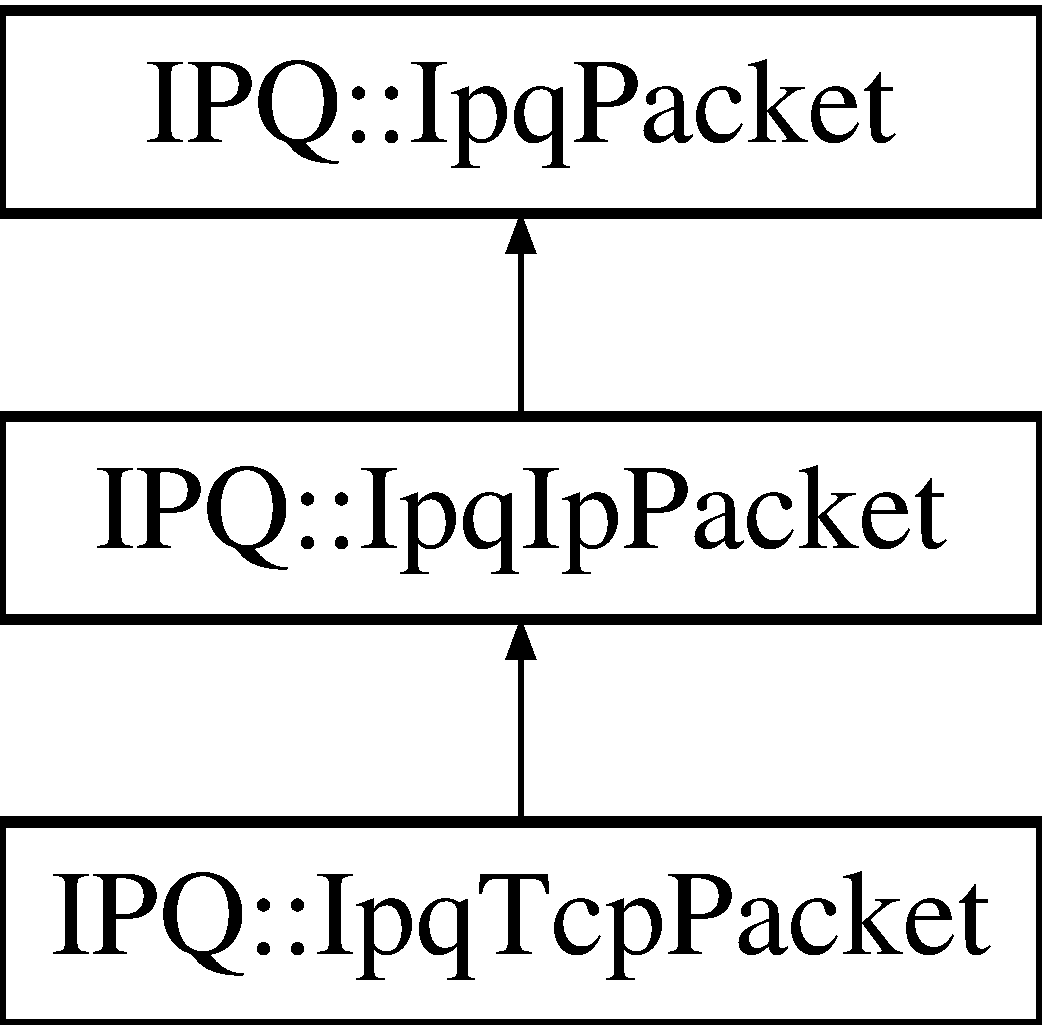
\includegraphics[height=3.000000cm]{classIPQ_1_1IpqTcpPacket}
\end{center}
\end{figure}
\subsection*{\-Public \-Member \-Functions}
\begin{DoxyCompactItemize}
\item 
in\-\_\-port\-\_\-t \hyperlink{classIPQ_1_1IpqTcpPacket_a970d80b0be1859f4b2a78d4784295872}{get\-Tcp\-Source} () const 
\begin{DoxyCompactList}\small\item\em \-Retrieve the \-T\-C\-P source port of a packet. \end{DoxyCompactList}\item 
in\-\_\-port\-\_\-t \hyperlink{classIPQ_1_1IpqTcpPacket_ad2fc945448bbfc68a682bf6cd354f35f}{get\-Tcp\-Dest} () const 
\begin{DoxyCompactList}\small\item\em \-Retrieve the \-T\-C\-P destination port of a packet. \end{DoxyCompactList}\item 
bool \hyperlink{classIPQ_1_1IpqTcpPacket_ac6e9e44d3f5059b6e5d17c74f5ab50df}{get\-Tcp\-Fin} () const 
\begin{DoxyCompactList}\small\item\em \-Retrieve the value of the \-T\-C\-P \-F\-I\-N flag. \end{DoxyCompactList}\item 
bool \hyperlink{classIPQ_1_1IpqTcpPacket_a39900fcdcc24d440616ad3ade555c8df}{get\-Tcp\-Syn} () const 
\begin{DoxyCompactList}\small\item\em \-Retrieve the value of the \-T\-C\-P \-S\-Y\-N flag. \end{DoxyCompactList}\item 
bool \hyperlink{classIPQ_1_1IpqTcpPacket_a7cb2b385f6fcd31d34c1e713c9f4221d}{get\-Tcp\-Rst} () const 
\begin{DoxyCompactList}\small\item\em \-Retrieve the value of the \-T\-C\-P \-R\-S\-T flag. \end{DoxyCompactList}\item 
bool \hyperlink{classIPQ_1_1IpqTcpPacket_a666820a105b69e9f01bd5fe7d5acb2da}{get\-Tcp\-Psh} () const 
\begin{DoxyCompactList}\small\item\em \-Retrieve the value of the \-T\-C\-P \-P\-S\-H flag. \end{DoxyCompactList}\item 
bool \hyperlink{classIPQ_1_1IpqTcpPacket_a45a7f295cfd6375e3a5a4b6e06ec9a47}{get\-Tcp\-Ack} () const 
\begin{DoxyCompactList}\small\item\em \-Retrieve the value of the \-T\-C\-P \-A\-C\-K flag. \end{DoxyCompactList}\item 
bool \hyperlink{classIPQ_1_1IpqTcpPacket_a28ed0e72fe9d25a7bbc5f03e1e91fcb9}{get\-Tcp\-Urg} () const 
\begin{DoxyCompactList}\small\item\em \-Retrieve the value of the \-T\-C\-P \-U\-R\-G flag. \end{DoxyCompactList}\item 
struct tcphdr \& \hyperlink{classIPQ_1_1IpqTcpPacket_a10987837a2b53336b43d059a74d00808}{get\-Tcp\-Header} () const 
\begin{DoxyCompactList}\small\item\em \-Retrieve the complete \-T\-C\-P header of a packet. \end{DoxyCompactList}\item 
struct tcphdr \& \hyperlink{classIPQ_1_1IpqTcpPacket_a170fa508e31ca3d0330f839224297240}{get\-Tcp\-Header} ()
\begin{DoxyCompactList}\small\item\em \-Retrieve the complete \-T\-C\-P header of a packet. \end{DoxyCompactList}\item 
const boost\-::uint8\-\_\-t $\ast$ \hyperlink{classIPQ_1_1IpqTcpPacket_ac56d211c471b6a721695f40762f7e411}{get\-Tcp\-Payload} (std\-::size\-\_\-t \&size) const 
\begin{DoxyCompactList}\small\item\em \-Retrive the \-T\-C\-P payload of a packet. \end{DoxyCompactList}\item 
boost\-::uint8\-\_\-t $\ast$ \hyperlink{classIPQ_1_1IpqTcpPacket_a9b90d7f24d2a48ce5627df74bdd05270}{get\-Tcp\-Payload} (std\-::size\-\_\-t \&size)
\begin{DoxyCompactList}\small\item\em \-Retrive the \-I\-P payload of a packet. \end{DoxyCompactList}\item 
virtual void \hyperlink{classIPQ_1_1IpqTcpPacket_a751f98aa2aafbe6796bf3a82d7273bec}{print} (std\-::ostream \&out) const 
\begin{DoxyCompactList}\small\item\em \-Print a \-T\-C\-P packet to stdout in an easy-\/to-\/read format. \end{DoxyCompactList}\item 
virtual \hyperlink{classIPQ_1_1IpqTcpPacket_a0e8394e3fa7f84f86009a5e7d6ffd5d0}{$\sim$\-Ipq\-Tcp\-Packet} ()
\begin{DoxyCompactList}\small\item\em \-Destructor for \hyperlink{classIPQ_1_1IpqTcpPacket}{\-Ipq\-Tcp\-Packet}. \end{DoxyCompactList}\item 
in\-\_\-addr\-\_\-t \hyperlink{classIPQ_1_1IpqIpPacket_a4708c5a987eb9796566e2b3bdd072589}{get\-Ip\-Source} () const 
\begin{DoxyCompactList}\small\item\em \-Retrieve the source \-I\-P address of a packet. \end{DoxyCompactList}\item 
in\-\_\-addr\-\_\-t \hyperlink{classIPQ_1_1IpqIpPacket_a056bedcbf7998452d147f2d2ef68b611}{get\-Ip\-Dest} () const 
\begin{DoxyCompactList}\small\item\em \-Retrieve the destination \-I\-P address of a packet. \end{DoxyCompactList}\item 
boost\-::uint8\-\_\-t \hyperlink{classIPQ_1_1IpqIpPacket_aefa78bb7a89a337bb0c1d88c02d6d5cd}{get\-Protocol} () const 
\begin{DoxyCompactList}\small\item\em \-Retrieve the encapsulated protocol number of a packet. \end{DoxyCompactList}\item 
boost\-::uint16\-\_\-t \hyperlink{classIPQ_1_1IpqIpPacket_a937be4034dafdce171b7e90ae14f09d4}{get\-Id} () const 
\begin{DoxyCompactList}\small\item\em \-Retrieve the \-I\-P \-I\-D of a packet. \end{DoxyCompactList}\item 
boost\-::uint16\-\_\-t \hyperlink{classIPQ_1_1IpqIpPacket_a97e6e13ede2c6c6f028ee0eb1130600b}{get\-Frag\-Offset} () const 
\begin{DoxyCompactList}\small\item\em \-Retrieve the fragment offset of a packet, in bytes. \end{DoxyCompactList}\item 
bool \hyperlink{classIPQ_1_1IpqIpPacket_a76e0d09916fc816df3dab46cb29d479f}{get\-More\-Frags} () const 
\begin{DoxyCompactList}\small\item\em \-Retrieve the \char`\"{}more fragments to follow\char`\"{} flag of a packet. \end{DoxyCompactList}\item 
struct iphdr \& \hyperlink{classIPQ_1_1IpqIpPacket_abf46954191d96b4e2fe136f79ba6c8ac}{get\-Ip\-Header} () const 
\begin{DoxyCompactList}\small\item\em \-Retrieve the complete \-I\-P header of a packet. \end{DoxyCompactList}\item 
struct iphdr \& \hyperlink{classIPQ_1_1IpqIpPacket_aa6e89b7927e748d00b9562e85192b492}{get\-Ip\-Header} ()
\begin{DoxyCompactList}\small\item\em \-Retrieve the complete \-I\-P header of a packet. \end{DoxyCompactList}\item 
const boost\-::uint8\-\_\-t $\ast$ \hyperlink{classIPQ_1_1IpqIpPacket_adc020ff0aceeba0577e4bb90dcc6f86f}{get\-Ip\-Payload} (std\-::size\-\_\-t \&size) const 
\begin{DoxyCompactList}\small\item\em \-Retrive the \-I\-P payload of a packet. \end{DoxyCompactList}\item 
boost\-::uint8\-\_\-t $\ast$ \hyperlink{classIPQ_1_1IpqIpPacket_a47343dd1a4fc52c8fda6de4aa313a688}{get\-Ip\-Payload} (std\-::size\-\_\-t \&size)
\begin{DoxyCompactList}\small\item\em \-Retrive the \-I\-P payload of a packet. \end{DoxyCompactList}\item 
unsigned long \hyperlink{classIPQ_1_1IpqPacket_ac3cbbe2b61e12730ffe231fa19c96e5a}{get\-Nf\-Id} () const 
\begin{DoxyCompactList}\small\item\em \-Retrieve the \-Netfilter \-I\-D of a packet. \end{DoxyCompactList}\item 
unsigned long \hyperlink{classIPQ_1_1IpqPacket_ab97f0a4348e53cb69ed1da74e422dc78}{get\-Nf\-Mark} () const 
\begin{DoxyCompactList}\small\item\em \-Retrieve the \-Netfilter mark value of a packet. \end{DoxyCompactList}\item 
void \hyperlink{classIPQ_1_1IpqPacket_a430ce4f89e651724efdf56c9c1b1647e}{get\-Timestamp} (struct timeval \&time) const 
\begin{DoxyCompactList}\small\item\em \-Retrieve the arrival time of a packet. \end{DoxyCompactList}\item 
unsigned \hyperlink{classIPQ_1_1IpqPacket_ae13884fedce165702f4b71e0e4d93c0b}{get\-Nf\-Hook} () const 
\begin{DoxyCompactList}\small\item\em \-Retrieve the number of the \-Netfilter hook on which the packet arrived. \end{DoxyCompactList}\item 
const char(\& \hyperlink{classIPQ_1_1IpqPacket_a4cf04ca5da28410f27d87edefd679532}{get\-Indev\-Name} () const)\mbox{[}\-I\-F\-N\-A\-M\-S\-I\-Z\mbox{]}
\begin{DoxyCompactList}\small\item\em \-Retrieve the name of the interface on which the packet arrived, if available. \end{DoxyCompactList}\item 
const char(\& \hyperlink{classIPQ_1_1IpqPacket_a46dced8057de3bba7abfaaa63d7afcd4}{get\-Outdev\-Name} () const)\mbox{[}\-I\-F\-N\-A\-M\-S\-I\-Z\mbox{]}
\begin{DoxyCompactList}\small\item\em \-Retrieve the name of the interface on which the packet will leave, if available. \end{DoxyCompactList}\item 
unsigned short \hyperlink{classIPQ_1_1IpqPacket_ae150e294f043f4c699231a85d3b1ae0f}{get\-Hw\-Protocol} () const 
\begin{DoxyCompactList}\small\item\em \-Retrieve the hardware protocol number of the packet. \end{DoxyCompactList}\item 
unsigned short \hyperlink{classIPQ_1_1IpqPacket_ab6b76b146111c7ad11b96e87efe6634c}{get\-Hw\-Type} () const 
\begin{DoxyCompactList}\small\item\em \-Retrieve the hardware type on which the packet arrived. \end{DoxyCompactList}\item 
const unsigned char(\& \hyperlink{classIPQ_1_1IpqPacket_a8582ae732d6b66ca1f5201994159a84a}{get\-Hw\-Source} (unsigned short \&addrlen) const)\mbox{[}8\mbox{]}
\begin{DoxyCompactList}\small\item\em \-Retrieve the source hardware address of the packet. \end{DoxyCompactList}\item 
const boost\-::uint8\-\_\-t $\ast$ \hyperlink{classIPQ_1_1IpqPacket_a6dd7baeec66082658d882bff8862eb6c}{get\-Packet} (std\-::size\-\_\-t \&size) const 
\begin{DoxyCompactList}\small\item\em \-Retrieve the packet. \end{DoxyCompactList}\item 
boost\-::uint8\-\_\-t $\ast$ \hyperlink{classIPQ_1_1IpqPacket_a0bf3344a9eed5e2f6bc20890ffffe26e}{get\-Packet} (std\-::size\-\_\-t \&size)
\begin{DoxyCompactList}\small\item\em \-Retrieve the packet. \end{DoxyCompactList}\end{DoxyCompactItemize}
\subsection*{\-Protected \-Member \-Functions}
\begin{DoxyCompactItemize}
\item 
\hyperlink{classIPQ_1_1IpqTcpPacket_a3b8faa690b49ce88bbc83cca7831f92e}{\-Ipq\-Tcp\-Packet} (\hyperlink{classLibWheel_1_1auto__array}{\-Lib\-Wheel\-::auto\-\_\-array}$<$ boost\-::uint8\-\_\-t $>$ buf, std\-::size\-\_\-t buflen)
\begin{DoxyCompactList}\small\item\em \-Constructor for \hyperlink{classIPQ_1_1IpqTcpPacket}{\-Ipq\-Tcp\-Packet}. \end{DoxyCompactList}\item 
struct tcphdr \& \hyperlink{classIPQ_1_1IpqTcpPacket_afa068ad5cdd7b67ad42acc2377a979ce}{do\-Get\-Tcp\-Header} () const 
\begin{DoxyCompactList}\small\item\em \-Retrieve the complete \-T\-C\-P header of a packet. \end{DoxyCompactList}\item 
boost\-::uint8\-\_\-t $\ast$ \hyperlink{classIPQ_1_1IpqTcpPacket_ae647a5597a784ec88cdc2091457d0607}{do\-Get\-Tcp\-Payload} (std\-::size\-\_\-t \&size) const 
\begin{DoxyCompactList}\small\item\em \-Retrive the \-T\-C\-P payload of a packet. \end{DoxyCompactList}\item 
virtual void \hyperlink{classIPQ_1_1IpqTcpPacket_aa3c42606d262b29f2b4bef459f34dd90}{update\-Checksums} ()
\begin{DoxyCompactList}\small\item\em \-Update the checksums on an \-T\-C\-P packet. \end{DoxyCompactList}\item 
struct iphdr \& \hyperlink{classIPQ_1_1IpqIpPacket_a6be0afa1f616cbe7722ef817a65e24dc}{do\-Get\-Ip\-Header} () const 
\begin{DoxyCompactList}\small\item\em \-Retrieve the complete \-I\-P header of a packet. \end{DoxyCompactList}\item 
boost\-::uint8\-\_\-t $\ast$ \hyperlink{classIPQ_1_1IpqIpPacket_ab78709e0712a1912d19114f815407303}{do\-Get\-Ip\-Payload} (std\-::size\-\_\-t \&size) const 
\begin{DoxyCompactList}\small\item\em \-Retrive the \-I\-P payload of a packet. \end{DoxyCompactList}\item 
boost\-::uint8\-\_\-t $\ast$ \hyperlink{classIPQ_1_1IpqPacket_a7b8f489a9cec36058eaee43f6566a999}{do\-Get\-Packet} (std\-::size\-\_\-t \&size) const 
\begin{DoxyCompactList}\small\item\em \-Retrieve the packet. \end{DoxyCompactList}\end{DoxyCompactItemize}
\subsection*{\-Static \-Protected \-Member \-Functions}
\begin{DoxyCompactItemize}
\item 
static \hyperlink{classIPQ_1_1IpqPacket}{\-Ipq\-Packet} $\ast$ \hyperlink{classIPQ_1_1IpqPacket_adf6099052730113814e9fe7312ec7b8c}{create\-Packet} (\hyperlink{classLibWheel_1_1auto__array}{\-Lib\-Wheel\-::auto\-\_\-array}$<$ boost\-::uint8\-\_\-t $>$ buf, std\-::size\-\_\-t buflen)
\begin{DoxyCompactList}\small\item\em \-Create an \hyperlink{classIPQ_1_1IpqPacket}{\-Ipq\-Packet} or one of its subclasses from a libipq packet message. \end{DoxyCompactList}\end{DoxyCompactItemize}
\subsection*{\-Protected \-Attributes}
\begin{DoxyCompactItemize}
\item 
\hyperlink{classLibWheel_1_1auto__array}{\-Lib\-Wheel\-::auto\-\_\-array}\*
$<$ boost\-::uint8\-\_\-t $>$ \hyperlink{classIPQ_1_1IpqPacket_a2bdf247f13a3e9f86e9e3846e6a9cb45}{packet}
\begin{DoxyCompactList}\small\item\em \-The packet message received from kernelspace. \end{DoxyCompactList}\item 
std\-::size\-\_\-t \hyperlink{classIPQ_1_1IpqPacket_a9b448a070c5ae499e32d2af5a190b86d}{packet\-Len}
\begin{DoxyCompactList}\small\item\em the length of the packet message in \hyperlink{classIPQ_1_1IpqPacket_a2bdf247f13a3e9f86e9e3846e6a9cb45}{\-Ipq\-Packet\-::packet}, in bytes. \end{DoxyCompactList}\item 
bool \hyperlink{classIPQ_1_1IpqPacket_a00acebf51531043a8536f20bb9412d61}{dirty}
\begin{DoxyCompactList}\small\item\em {\bfseries true} if the packet has been modified but checksums have not been updated; {\bfseries false} otherwise. \end{DoxyCompactList}\end{DoxyCompactItemize}
\subsection*{\-Friends}
\begin{DoxyCompactItemize}
\item 
\hyperlink{classIPQ_1_1IpqPacket}{\-Ipq\-Packet} $\ast$ \hyperlink{classIPQ_1_1IpqTcpPacket_af2019ef9442b13f8da0f53a082a9b308}{\-Ipq\-Packet\-::create\-Packet} (\hyperlink{classLibWheel_1_1auto__array}{\-Lib\-Wheel\-::auto\-\_\-array}$<$ boost\-::uint8\-\_\-t $>$, std\-::size\-\_\-t)
\begin{DoxyCompactList}\small\item\em \-Allow \-Ipq\-Socket\-::create\-Packet() to access the contstructor. \end{DoxyCompactList}\end{DoxyCompactItemize}


\subsection{\-Detailed \-Description}
\-An complete \-I\-Pv4/\-T\-C\-P packet that was received via \hyperlink{classIPQ_1_1IpqSocket}{\-Ipq\-Socket}. 

\-Contains \-T\-C\-P header fields and the \-T\-C\-P payload. 

\subsection{\-Constructor \& \-Destructor \-Documentation}
\hypertarget{classIPQ_1_1IpqTcpPacket_a0e8394e3fa7f84f86009a5e7d6ffd5d0}{
\index{\-I\-P\-Q\-::\-Ipq\-Tcp\-Packet@{\-I\-P\-Q\-::\-Ipq\-Tcp\-Packet}!$\sim$\-Ipq\-Tcp\-Packet@{$\sim$\-Ipq\-Tcp\-Packet}}
\index{$\sim$\-Ipq\-Tcp\-Packet@{$\sim$\-Ipq\-Tcp\-Packet}!IPQ::IpqTcpPacket@{\-I\-P\-Q\-::\-Ipq\-Tcp\-Packet}}
\subsubsection[{$\sim$\-Ipq\-Tcp\-Packet}]{\setlength{\rightskip}{0pt plus 5cm}\-I\-P\-Q\-::\-Ipq\-Tcp\-Packet\-::$\sim$\-Ipq\-Tcp\-Packet (
\begin{DoxyParamCaption}
{}
\end{DoxyParamCaption}
)\hspace{0.3cm}{\ttfamily  \mbox{[}virtual\mbox{]}}}}
\label{classIPQ_1_1IpqTcpPacket_a0e8394e3fa7f84f86009a5e7d6ffd5d0}


\-Destructor for \hyperlink{classIPQ_1_1IpqTcpPacket}{\-Ipq\-Tcp\-Packet}. 



\-Definition at line 1139 of file \-I\-P\-Q.\-cpp.

\hypertarget{classIPQ_1_1IpqTcpPacket_a3b8faa690b49ce88bbc83cca7831f92e}{
\index{\-I\-P\-Q\-::\-Ipq\-Tcp\-Packet@{\-I\-P\-Q\-::\-Ipq\-Tcp\-Packet}!\-Ipq\-Tcp\-Packet@{\-Ipq\-Tcp\-Packet}}
\index{\-Ipq\-Tcp\-Packet@{\-Ipq\-Tcp\-Packet}!IPQ::IpqTcpPacket@{\-I\-P\-Q\-::\-Ipq\-Tcp\-Packet}}
\subsubsection[{\-Ipq\-Tcp\-Packet}]{\setlength{\rightskip}{0pt plus 5cm}\-I\-P\-Q\-::\-Ipq\-Tcp\-Packet\-::\-Ipq\-Tcp\-Packet (
\begin{DoxyParamCaption}
\item[{{\bf \-Lib\-Wheel\-::auto\-\_\-array}$<$ boost\-::uint8\-\_\-t $>$}]{buf, }
\item[{std\-::size\-\_\-t}]{buflen}
\end{DoxyParamCaption}
)\hspace{0.3cm}{\ttfamily  \mbox{[}protected\mbox{]}}}}
\label{classIPQ_1_1IpqTcpPacket_a3b8faa690b49ce88bbc83cca7831f92e}


\-Constructor for \hyperlink{classIPQ_1_1IpqTcpPacket}{\-Ipq\-Tcp\-Packet}. 

\-Initializes an \hyperlink{classIPQ_1_1IpqTcpPacket}{\-Ipq\-Tcp\-Packet} from a libipq packet message. 

\-Definition at line 1147 of file \-I\-P\-Q.\-cpp.



\subsection{\-Member \-Function \-Documentation}
\hypertarget{classIPQ_1_1IpqPacket_adf6099052730113814e9fe7312ec7b8c}{
\index{\-I\-P\-Q\-::\-Ipq\-Tcp\-Packet@{\-I\-P\-Q\-::\-Ipq\-Tcp\-Packet}!create\-Packet@{create\-Packet}}
\index{create\-Packet@{create\-Packet}!IPQ::IpqTcpPacket@{\-I\-P\-Q\-::\-Ipq\-Tcp\-Packet}}
\subsubsection[{create\-Packet}]{\setlength{\rightskip}{0pt plus 5cm}{\bf \-Ipq\-Packet} $\ast$ \-I\-P\-Q\-::\-Ipq\-Packet\-::create\-Packet (
\begin{DoxyParamCaption}
\item[{{\bf \-Lib\-Wheel\-::auto\-\_\-array}$<$ boost\-::uint8\-\_\-t $>$}]{buf, }
\item[{std\-::size\-\_\-t}]{buflen}
\end{DoxyParamCaption}
)\hspace{0.3cm}{\ttfamily  \mbox{[}static, protected, inherited\mbox{]}}}}
\label{classIPQ_1_1IpqPacket_adf6099052730113814e9fe7312ec7b8c}


\-Create an \hyperlink{classIPQ_1_1IpqPacket}{\-Ipq\-Packet} or one of its subclasses from a libipq packet message. 

\-A packet will be deemed to be an \-I\-Pv4 packet if it has a full \-I\-Pv4 header and the data length indicated by the header matches the packet's length. \-A packet will be deemed to be a \-T\-C\-P or \-U\-D\-P packet if it is an \-I\-Pv4 packet and it has a full \-T\-C\-P or \-U\-D\-P header. \begin{DoxyReturn}{\-Returns}
\-A pointer to a dynamically-\/allocated \hyperlink{classIPQ_1_1IpqPacket}{\-Ipq\-Packet}, or one of its subclasses. \-This pointer must be freed using {\bfseries delete}, and a verdict should be set on it using \hyperlink{classIPQ_1_1IpqSocket_a53e0f4e45363cbcd919a2d96ee7cf0a8}{\-Ipq\-Socket\-::send\-Response()}. 
\end{DoxyReturn}


\-Definition at line 731 of file \-I\-P\-Q.\-cpp.



\-References \-Lib\-Wheel\-::auto\-\_\-array\-::get(), and \-I\-P\-Q\-::\-Ipq\-Packet\-::\-Ipq\-Packet().



\-Referenced by \-I\-P\-Q\-::\-Ipq\-Socket\-::recv\-Packet().

\hypertarget{classIPQ_1_1IpqIpPacket_a6be0afa1f616cbe7722ef817a65e24dc}{
\index{\-I\-P\-Q\-::\-Ipq\-Tcp\-Packet@{\-I\-P\-Q\-::\-Ipq\-Tcp\-Packet}!do\-Get\-Ip\-Header@{do\-Get\-Ip\-Header}}
\index{do\-Get\-Ip\-Header@{do\-Get\-Ip\-Header}!IPQ::IpqTcpPacket@{\-I\-P\-Q\-::\-Ipq\-Tcp\-Packet}}
\subsubsection[{do\-Get\-Ip\-Header}]{\setlength{\rightskip}{0pt plus 5cm}struct iphdr \& \-I\-P\-Q\-::\-Ipq\-Ip\-Packet\-::do\-Get\-Ip\-Header (
\begin{DoxyParamCaption}
{}
\end{DoxyParamCaption}
) const\hspace{0.3cm}{\ttfamily  \mbox{[}read, protected, inherited\mbox{]}}}}
\label{classIPQ_1_1IpqIpPacket_a6be0afa1f616cbe7722ef817a65e24dc}


\-Retrieve the complete \-I\-P header of a packet. 

\-A reference to the packet's \-I\-P header. 

\-Definition at line 928 of file \-I\-P\-Q.\-cpp.



\-References \-I\-P\-Q\-::\-Ipq\-Packet\-::packet, and \-Lib\-Wheel\-::auto\-\_\-array\-::get().



\-Referenced by \-I\-P\-Q\-::\-Ipq\-Ip\-Packet\-::get\-Ip\-Header().

\hypertarget{classIPQ_1_1IpqIpPacket_ab78709e0712a1912d19114f815407303}{
\index{\-I\-P\-Q\-::\-Ipq\-Tcp\-Packet@{\-I\-P\-Q\-::\-Ipq\-Tcp\-Packet}!do\-Get\-Ip\-Payload@{do\-Get\-Ip\-Payload}}
\index{do\-Get\-Ip\-Payload@{do\-Get\-Ip\-Payload}!IPQ::IpqTcpPacket@{\-I\-P\-Q\-::\-Ipq\-Tcp\-Packet}}
\subsubsection[{do\-Get\-Ip\-Payload}]{\setlength{\rightskip}{0pt plus 5cm}boost\-::uint8\-\_\-t $\ast$ \-I\-P\-Q\-::\-Ipq\-Ip\-Packet\-::do\-Get\-Ip\-Payload (
\begin{DoxyParamCaption}
\item[{std\-::size\-\_\-t \&}]{size}
\end{DoxyParamCaption}
) const\hspace{0.3cm}{\ttfamily  \mbox{[}protected, inherited\mbox{]}}}}
\label{classIPQ_1_1IpqIpPacket_ab78709e0712a1912d19114f815407303}


\-Retrive the \-I\-P payload of a packet. 


\begin{DoxyParams}[1]{\-Parameters}
\mbox{\tt out}  & {\em size} & \-A reference to a location to store the packet's \-I\-P payload size, in bytes.. \\
\hline
\end{DoxyParams}
\begin{DoxyReturn}{\-Returns}
\-A const pointer to the packet's \-I\-P payload. 
\end{DoxyReturn}


\-Definition at line 941 of file \-I\-P\-Q.\-cpp.



\-References \-I\-P\-Q\-::\-Ipq\-Packet\-::packet, and \-Lib\-Wheel\-::auto\-\_\-array\-::get().



\-Referenced by \-I\-P\-Q\-::\-Ipq\-Ip\-Packet\-::get\-Ip\-Payload().

\hypertarget{classIPQ_1_1IpqPacket_a7b8f489a9cec36058eaee43f6566a999}{
\index{\-I\-P\-Q\-::\-Ipq\-Tcp\-Packet@{\-I\-P\-Q\-::\-Ipq\-Tcp\-Packet}!do\-Get\-Packet@{do\-Get\-Packet}}
\index{do\-Get\-Packet@{do\-Get\-Packet}!IPQ::IpqTcpPacket@{\-I\-P\-Q\-::\-Ipq\-Tcp\-Packet}}
\subsubsection[{do\-Get\-Packet}]{\setlength{\rightskip}{0pt plus 5cm}boost\-::uint8\-\_\-t $\ast$ \-I\-P\-Q\-::\-Ipq\-Packet\-::do\-Get\-Packet (
\begin{DoxyParamCaption}
\item[{std\-::size\-\_\-t \&}]{size}
\end{DoxyParamCaption}
) const\hspace{0.3cm}{\ttfamily  \mbox{[}protected, inherited\mbox{]}}}}
\label{classIPQ_1_1IpqPacket_a7b8f489a9cec36058eaee43f6566a999}


\-Retrieve the packet. 

\-It will only be available if the copy mode on the libipq handle used to receive it was \hyperlink{classIPQ_1_1IpqSocket_afee6d75480079906ecf6544f8467e0ccafc1e90369658a807b2c970d3e15b01d4}{\-Ipq\-Socket\-::\-P\-A\-C\-K\-E\-T} and the copy range was greater than zero. 
\begin{DoxyParams}[1]{\-Parameters}
\mbox{\tt out}  & {\em size} & \-A reference to a location to write the length of the payload, in bytes. \\
\hline
\end{DoxyParams}
\begin{DoxyReturn}{\-Returns}
\-A pointer to the packet. 
\end{DoxyReturn}


\-Definition at line 703 of file \-I\-P\-Q.\-cpp.



\-References \-I\-P\-Q\-::\-Ipq\-Packet\-::packet, and \-Lib\-Wheel\-::auto\-\_\-array\-::get().



\-Referenced by \-I\-P\-Q\-::\-Ipq\-Packet\-::get\-Packet().

\hypertarget{classIPQ_1_1IpqTcpPacket_afa068ad5cdd7b67ad42acc2377a979ce}{
\index{\-I\-P\-Q\-::\-Ipq\-Tcp\-Packet@{\-I\-P\-Q\-::\-Ipq\-Tcp\-Packet}!do\-Get\-Tcp\-Header@{do\-Get\-Tcp\-Header}}
\index{do\-Get\-Tcp\-Header@{do\-Get\-Tcp\-Header}!IPQ::IpqTcpPacket@{\-I\-P\-Q\-::\-Ipq\-Tcp\-Packet}}
\subsubsection[{do\-Get\-Tcp\-Header}]{\setlength{\rightskip}{0pt plus 5cm}struct tcphdr \& \-I\-P\-Q\-::\-Ipq\-Tcp\-Packet\-::do\-Get\-Tcp\-Header (
\begin{DoxyParamCaption}
{}
\end{DoxyParamCaption}
) const\hspace{0.3cm}{\ttfamily  \mbox{[}read, protected\mbox{]}}}}
\label{classIPQ_1_1IpqTcpPacket_afa068ad5cdd7b67ad42acc2377a979ce}


\-Retrieve the complete \-T\-C\-P header of a packet. 

\-A reference to the packet's \-T\-C\-P header. 

\-Definition at line 1157 of file \-I\-P\-Q.\-cpp.



\-References \-I\-P\-Q\-::\-Ipq\-Packet\-::packet, and \-Lib\-Wheel\-::auto\-\_\-array\-::get().



\-Referenced by get\-Tcp\-Header().

\hypertarget{classIPQ_1_1IpqTcpPacket_ae647a5597a784ec88cdc2091457d0607}{
\index{\-I\-P\-Q\-::\-Ipq\-Tcp\-Packet@{\-I\-P\-Q\-::\-Ipq\-Tcp\-Packet}!do\-Get\-Tcp\-Payload@{do\-Get\-Tcp\-Payload}}
\index{do\-Get\-Tcp\-Payload@{do\-Get\-Tcp\-Payload}!IPQ::IpqTcpPacket@{\-I\-P\-Q\-::\-Ipq\-Tcp\-Packet}}
\subsubsection[{do\-Get\-Tcp\-Payload}]{\setlength{\rightskip}{0pt plus 5cm}boost\-::uint8\-\_\-t $\ast$ \-I\-P\-Q\-::\-Ipq\-Tcp\-Packet\-::do\-Get\-Tcp\-Payload (
\begin{DoxyParamCaption}
\item[{std\-::size\-\_\-t \&}]{size}
\end{DoxyParamCaption}
) const\hspace{0.3cm}{\ttfamily  \mbox{[}protected\mbox{]}}}}
\label{classIPQ_1_1IpqTcpPacket_ae647a5597a784ec88cdc2091457d0607}


\-Retrive the \-T\-C\-P payload of a packet. 


\begin{DoxyParams}[1]{\-Parameters}
\mbox{\tt out}  & {\em size} & \-A reference to a location to store the packet's \-T\-C\-P payload size, in bytes.. \\
\hline
\end{DoxyParams}
\begin{DoxyReturn}{\-Returns}
\-A pointer to the packet's \-T\-C\-P payload. 
\end{DoxyReturn}


\-Definition at line 1171 of file \-I\-P\-Q.\-cpp.



\-References \-I\-P\-Q\-::\-Ipq\-Packet\-::packet, and \-Lib\-Wheel\-::auto\-\_\-array\-::get().



\-Referenced by get\-Tcp\-Payload().

\hypertarget{classIPQ_1_1IpqIpPacket_a97e6e13ede2c6c6f028ee0eb1130600b}{
\index{\-I\-P\-Q\-::\-Ipq\-Tcp\-Packet@{\-I\-P\-Q\-::\-Ipq\-Tcp\-Packet}!get\-Frag\-Offset@{get\-Frag\-Offset}}
\index{get\-Frag\-Offset@{get\-Frag\-Offset}!IPQ::IpqTcpPacket@{\-I\-P\-Q\-::\-Ipq\-Tcp\-Packet}}
\subsubsection[{get\-Frag\-Offset}]{\setlength{\rightskip}{0pt plus 5cm}boost\-::uint16\-\_\-t \-I\-P\-Q\-::\-Ipq\-Ip\-Packet\-::get\-Frag\-Offset (
\begin{DoxyParamCaption}
{}
\end{DoxyParamCaption}
) const\hspace{0.3cm}{\ttfamily  \mbox{[}inherited\mbox{]}}}}
\label{classIPQ_1_1IpqIpPacket_a97e6e13ede2c6c6f028ee0eb1130600b}


\-Retrieve the fragment offset of a packet, in bytes. 

\-If not zero, then this is a non-\/leading fragment. \begin{DoxyReturn}{\-Returns}
\-The packet's fragment offset. 
\end{DoxyReturn}


\-Definition at line 817 of file \-I\-P\-Q.\-cpp.



\-References \-I\-P\-Q\-::\-Ipq\-Ip\-Packet\-::get\-Ip\-Header().



\-Referenced by \-I\-P\-Q\-::\-Ipq\-Ip\-Packet\-::print(), and \-N\-E\-R\-D\-::\-Connection\-Server\-::handle\-Packet().

\hypertarget{classIPQ_1_1IpqPacket_ae150e294f043f4c699231a85d3b1ae0f}{
\index{\-I\-P\-Q\-::\-Ipq\-Tcp\-Packet@{\-I\-P\-Q\-::\-Ipq\-Tcp\-Packet}!get\-Hw\-Protocol@{get\-Hw\-Protocol}}
\index{get\-Hw\-Protocol@{get\-Hw\-Protocol}!IPQ::IpqTcpPacket@{\-I\-P\-Q\-::\-Ipq\-Tcp\-Packet}}
\subsubsection[{get\-Hw\-Protocol}]{\setlength{\rightskip}{0pt plus 5cm}unsigned short \-I\-P\-Q\-::\-Ipq\-Packet\-::get\-Hw\-Protocol (
\begin{DoxyParamCaption}
{}
\end{DoxyParamCaption}
) const\hspace{0.3cm}{\ttfamily  \mbox{[}inherited\mbox{]}}}}
\label{classIPQ_1_1IpqPacket_ae150e294f043f4c699231a85d3b1ae0f}


\-Retrieve the hardware protocol number of the packet. 

\begin{DoxyReturn}{\-Returns}
\-The packet's hardware protocol number. 
\end{DoxyReturn}


\-Definition at line 585 of file \-I\-P\-Q.\-cpp.



\-References \-I\-P\-Q\-::\-Ipq\-Packet\-::packet, and \-Lib\-Wheel\-::auto\-\_\-array\-::get().



\-Referenced by \-I\-P\-Q\-::\-Ipq\-Packet\-::print().

\hypertarget{classIPQ_1_1IpqPacket_a8582ae732d6b66ca1f5201994159a84a}{
\index{\-I\-P\-Q\-::\-Ipq\-Tcp\-Packet@{\-I\-P\-Q\-::\-Ipq\-Tcp\-Packet}!get\-Hw\-Source@{get\-Hw\-Source}}
\index{get\-Hw\-Source@{get\-Hw\-Source}!IPQ::IpqTcpPacket@{\-I\-P\-Q\-::\-Ipq\-Tcp\-Packet}}
\subsubsection[{get\-Hw\-Source}]{\setlength{\rightskip}{0pt plus 5cm}const unsigned char(\& \-I\-P\-Q\-::\-Ipq\-Packet\-::get\-Hw\-Source (
\begin{DoxyParamCaption}
\item[{unsigned short \&}]{addrlen}
\end{DoxyParamCaption}
))\mbox{[}8\mbox{]}\hspace{0.3cm}{\ttfamily  \mbox{[}inherited\mbox{]}}}}
\label{classIPQ_1_1IpqPacket_a8582ae732d6b66ca1f5201994159a84a}


\-Retrieve the source hardware address of the packet. 


\begin{DoxyParams}[1]{\-Parameters}
\mbox{\tt out}  & {\em addrlen} & \-A reference to a location to write the actual length of the address, in bytes. \\
\hline
\end{DoxyParams}
\begin{DoxyReturn}{\-Returns}
\-A reference to the packet's source hardware address. 
\end{DoxyReturn}


\-Definition at line 608 of file \-I\-P\-Q.\-cpp.



\-Referenced by \-I\-P\-Q\-::\-Ipq\-Packet\-::print().

\hypertarget{classIPQ_1_1IpqPacket_ab6b76b146111c7ad11b96e87efe6634c}{
\index{\-I\-P\-Q\-::\-Ipq\-Tcp\-Packet@{\-I\-P\-Q\-::\-Ipq\-Tcp\-Packet}!get\-Hw\-Type@{get\-Hw\-Type}}
\index{get\-Hw\-Type@{get\-Hw\-Type}!IPQ::IpqTcpPacket@{\-I\-P\-Q\-::\-Ipq\-Tcp\-Packet}}
\subsubsection[{get\-Hw\-Type}]{\setlength{\rightskip}{0pt plus 5cm}unsigned short \-I\-P\-Q\-::\-Ipq\-Packet\-::get\-Hw\-Type (
\begin{DoxyParamCaption}
{}
\end{DoxyParamCaption}
) const\hspace{0.3cm}{\ttfamily  \mbox{[}inherited\mbox{]}}}}
\label{classIPQ_1_1IpqPacket_ab6b76b146111c7ad11b96e87efe6634c}


\-Retrieve the hardware type on which the packet arrived. 

\begin{DoxyReturn}{\-Returns}
\-The packet's arrival hardware type. 
\end{DoxyReturn}


\-Definition at line 596 of file \-I\-P\-Q.\-cpp.



\-References \-I\-P\-Q\-::\-Ipq\-Packet\-::packet, and \-Lib\-Wheel\-::auto\-\_\-array\-::get().



\-Referenced by \-I\-P\-Q\-::\-Ipq\-Packet\-::print().

\hypertarget{classIPQ_1_1IpqIpPacket_a937be4034dafdce171b7e90ae14f09d4}{
\index{\-I\-P\-Q\-::\-Ipq\-Tcp\-Packet@{\-I\-P\-Q\-::\-Ipq\-Tcp\-Packet}!get\-Id@{get\-Id}}
\index{get\-Id@{get\-Id}!IPQ::IpqTcpPacket@{\-I\-P\-Q\-::\-Ipq\-Tcp\-Packet}}
\subsubsection[{get\-Id}]{\setlength{\rightskip}{0pt plus 5cm}boost\-::uint16\-\_\-t \-I\-P\-Q\-::\-Ipq\-Ip\-Packet\-::get\-Id (
\begin{DoxyParamCaption}
{}
\end{DoxyParamCaption}
) const\hspace{0.3cm}{\ttfamily  \mbox{[}inherited\mbox{]}}}}
\label{classIPQ_1_1IpqIpPacket_a937be4034dafdce171b7e90ae14f09d4}


\-Retrieve the \-I\-P \-I\-D of a packet. 

\begin{DoxyReturn}{\-Returns}
\-The packet's \-I\-P\-I\-D. 
\end{DoxyReturn}


\-Definition at line 805 of file \-I\-P\-Q.\-cpp.



\-References \-I\-P\-Q\-::\-Ipq\-Ip\-Packet\-::get\-Ip\-Header().



\-Referenced by \-I\-P\-Q\-::\-Ipq\-Ip\-Packet\-::print().

\hypertarget{classIPQ_1_1IpqPacket_a4cf04ca5da28410f27d87edefd679532}{
\index{\-I\-P\-Q\-::\-Ipq\-Tcp\-Packet@{\-I\-P\-Q\-::\-Ipq\-Tcp\-Packet}!get\-Indev\-Name@{get\-Indev\-Name}}
\index{get\-Indev\-Name@{get\-Indev\-Name}!IPQ::IpqTcpPacket@{\-I\-P\-Q\-::\-Ipq\-Tcp\-Packet}}
\subsubsection[{get\-Indev\-Name}]{\setlength{\rightskip}{0pt plus 5cm}const char(\& \-I\-P\-Q\-::\-Ipq\-Packet\-::get\-Indev\-Name (
\begin{DoxyParamCaption}
{}
\end{DoxyParamCaption}
))\mbox{[}\-I\-F\-N\-A\-M\-S\-I\-Z\mbox{]}\hspace{0.3cm}{\ttfamily  \mbox{[}inherited\mbox{]}}}}
\label{classIPQ_1_1IpqPacket_a4cf04ca5da28410f27d87edefd679532}


\-Retrieve the name of the interface on which the packet arrived, if available. 

\begin{DoxyReturn}{\-Returns}
\-A reference to the packet's arrival interface name. 
\end{DoxyReturn}


\-Definition at line 563 of file \-I\-P\-Q.\-cpp.



\-Referenced by \-I\-P\-Q\-::\-Ipq\-Packet\-::print().

\hypertarget{classIPQ_1_1IpqIpPacket_a056bedcbf7998452d147f2d2ef68b611}{
\index{\-I\-P\-Q\-::\-Ipq\-Tcp\-Packet@{\-I\-P\-Q\-::\-Ipq\-Tcp\-Packet}!get\-Ip\-Dest@{get\-Ip\-Dest}}
\index{get\-Ip\-Dest@{get\-Ip\-Dest}!IPQ::IpqTcpPacket@{\-I\-P\-Q\-::\-Ipq\-Tcp\-Packet}}
\subsubsection[{get\-Ip\-Dest}]{\setlength{\rightskip}{0pt plus 5cm}in\-\_\-addr\-\_\-t \-I\-P\-Q\-::\-Ipq\-Ip\-Packet\-::get\-Ip\-Dest (
\begin{DoxyParamCaption}
{}
\end{DoxyParamCaption}
) const\hspace{0.3cm}{\ttfamily  \mbox{[}inherited\mbox{]}}}}
\label{classIPQ_1_1IpqIpPacket_a056bedcbf7998452d147f2d2ef68b611}


\-Retrieve the destination \-I\-P address of a packet. 

\begin{DoxyReturn}{\-Returns}
\-The packet's destination \-I\-P address. 
\end{DoxyReturn}


\-Definition at line 783 of file \-I\-P\-Q.\-cpp.



\-References \-I\-P\-Q\-::\-Ipq\-Ip\-Packet\-::get\-Ip\-Header().



\-Referenced by \-I\-P\-Q\-::\-Ipq\-Socket\-::send\-Response(), \-I\-P\-Q\-::\-Ipq\-Ip\-Packet\-::print(), \-N\-E\-R\-D\-::\-Connection\-Server\-::handle\-Packet(), and \-N\-E\-R\-D\-::\-Connection\-Server\-::create\-Connection().

\hypertarget{classIPQ_1_1IpqIpPacket_abf46954191d96b4e2fe136f79ba6c8ac}{
\index{\-I\-P\-Q\-::\-Ipq\-Tcp\-Packet@{\-I\-P\-Q\-::\-Ipq\-Tcp\-Packet}!get\-Ip\-Header@{get\-Ip\-Header}}
\index{get\-Ip\-Header@{get\-Ip\-Header}!IPQ::IpqTcpPacket@{\-I\-P\-Q\-::\-Ipq\-Tcp\-Packet}}
\subsubsection[{get\-Ip\-Header}]{\setlength{\rightskip}{0pt plus 5cm}struct iphdr \& \-I\-P\-Q\-::\-Ipq\-Ip\-Packet\-::get\-Ip\-Header (
\begin{DoxyParamCaption}
{}
\end{DoxyParamCaption}
) const\hspace{0.3cm}{\ttfamily  \mbox{[}read, inherited\mbox{]}}}}
\label{classIPQ_1_1IpqIpPacket_abf46954191d96b4e2fe136f79ba6c8ac}


\-Retrieve the complete \-I\-P header of a packet. 

\-A const reference to the packet's \-I\-P header. 

\-Definition at line 840 of file \-I\-P\-Q.\-cpp.



\-References \-I\-P\-Q\-::\-Ipq\-Ip\-Packet\-::do\-Get\-Ip\-Header().



\-Referenced by \-I\-P\-Q\-::\-Ipq\-Ip\-Packet\-::get\-Ip\-Source(), \-I\-P\-Q\-::\-Ipq\-Ip\-Packet\-::get\-Ip\-Dest(), \-I\-P\-Q\-::\-Ipq\-Ip\-Packet\-::get\-Protocol(), \-I\-P\-Q\-::\-Ipq\-Ip\-Packet\-::get\-Id(), \-I\-P\-Q\-::\-Ipq\-Ip\-Packet\-::get\-Frag\-Offset(), \-I\-P\-Q\-::\-Ipq\-Ip\-Packet\-::get\-More\-Frags(), \-I\-P\-Q\-::\-Ipq\-Ip\-Packet\-::update\-Checksums(), update\-Checksums(), \-I\-P\-Q\-::\-Ipq\-Udp\-Packet\-::update\-Checksums(), and \-N\-E\-R\-D\-::\-Connection\-Server\-::handle\-Packet().

\hypertarget{classIPQ_1_1IpqIpPacket_aa6e89b7927e748d00b9562e85192b492}{
\index{\-I\-P\-Q\-::\-Ipq\-Tcp\-Packet@{\-I\-P\-Q\-::\-Ipq\-Tcp\-Packet}!get\-Ip\-Header@{get\-Ip\-Header}}
\index{get\-Ip\-Header@{get\-Ip\-Header}!IPQ::IpqTcpPacket@{\-I\-P\-Q\-::\-Ipq\-Tcp\-Packet}}
\subsubsection[{get\-Ip\-Header}]{\setlength{\rightskip}{0pt plus 5cm}struct iphdr \& \-I\-P\-Q\-::\-Ipq\-Ip\-Packet\-::get\-Ip\-Header (
\begin{DoxyParamCaption}
{}
\end{DoxyParamCaption}
)\hspace{0.3cm}{\ttfamily  \mbox{[}read, inherited\mbox{]}}}}
\label{classIPQ_1_1IpqIpPacket_aa6e89b7927e748d00b9562e85192b492}


\-Retrieve the complete \-I\-P header of a packet. 

\-A reference to the packet's \-I\-P header. \begin{DoxyNote}{\-Note}
\-This method sets the packet's dirty flag, requiring that the packet's checksums be recomputed before a verdict is set. 
\end{DoxyNote}


\-Definition at line 853 of file \-I\-P\-Q.\-cpp.



\-References \-I\-P\-Q\-::\-Ipq\-Packet\-::dirty, and \-I\-P\-Q\-::\-Ipq\-Ip\-Packet\-::do\-Get\-Ip\-Header().

\hypertarget{classIPQ_1_1IpqIpPacket_adc020ff0aceeba0577e4bb90dcc6f86f}{
\index{\-I\-P\-Q\-::\-Ipq\-Tcp\-Packet@{\-I\-P\-Q\-::\-Ipq\-Tcp\-Packet}!get\-Ip\-Payload@{get\-Ip\-Payload}}
\index{get\-Ip\-Payload@{get\-Ip\-Payload}!IPQ::IpqTcpPacket@{\-I\-P\-Q\-::\-Ipq\-Tcp\-Packet}}
\subsubsection[{get\-Ip\-Payload}]{\setlength{\rightskip}{0pt plus 5cm}const boost\-::uint8\-\_\-t $\ast$ \-I\-P\-Q\-::\-Ipq\-Ip\-Packet\-::get\-Ip\-Payload (
\begin{DoxyParamCaption}
\item[{std\-::size\-\_\-t \&}]{size}
\end{DoxyParamCaption}
) const\hspace{0.3cm}{\ttfamily  \mbox{[}inherited\mbox{]}}}}
\label{classIPQ_1_1IpqIpPacket_adc020ff0aceeba0577e4bb90dcc6f86f}


\-Retrive the \-I\-P payload of a packet. 


\begin{DoxyParams}[1]{\-Parameters}
\mbox{\tt out}  & {\em size} & \-A reference to a location to store the packet's \-I\-P payload size, in bytes.. \\
\hline
\end{DoxyParams}
\begin{DoxyReturn}{\-Returns}
\-A const pointer to the packet's \-I\-P payload. 
\end{DoxyReturn}


\-Definition at line 867 of file \-I\-P\-Q.\-cpp.



\-References \-I\-P\-Q\-::\-Ipq\-Ip\-Packet\-::do\-Get\-Ip\-Payload().

\hypertarget{classIPQ_1_1IpqIpPacket_a47343dd1a4fc52c8fda6de4aa313a688}{
\index{\-I\-P\-Q\-::\-Ipq\-Tcp\-Packet@{\-I\-P\-Q\-::\-Ipq\-Tcp\-Packet}!get\-Ip\-Payload@{get\-Ip\-Payload}}
\index{get\-Ip\-Payload@{get\-Ip\-Payload}!IPQ::IpqTcpPacket@{\-I\-P\-Q\-::\-Ipq\-Tcp\-Packet}}
\subsubsection[{get\-Ip\-Payload}]{\setlength{\rightskip}{0pt plus 5cm}boost\-::uint8\-\_\-t $\ast$ \-I\-P\-Q\-::\-Ipq\-Ip\-Packet\-::get\-Ip\-Payload (
\begin{DoxyParamCaption}
\item[{std\-::size\-\_\-t \&}]{size}
\end{DoxyParamCaption}
)\hspace{0.3cm}{\ttfamily  \mbox{[}inherited\mbox{]}}}}
\label{classIPQ_1_1IpqIpPacket_a47343dd1a4fc52c8fda6de4aa313a688}


\-Retrive the \-I\-P payload of a packet. 


\begin{DoxyParams}[1]{\-Parameters}
\mbox{\tt out}  & {\em size} & \-A reference to a location to store the packet's \-I\-P payload size, in bytes.. \\
\hline
\end{DoxyParams}
\begin{DoxyReturn}{\-Returns}
\-A pointer to the packet's \-I\-P payload. 
\end{DoxyReturn}
\begin{DoxyNote}{\-Note}
\-This method sets the packet's dirty flag, requiring that the packet's checksums be recomputed before a verdict is set. 
\end{DoxyNote}


\-Definition at line 882 of file \-I\-P\-Q.\-cpp.



\-References \-I\-P\-Q\-::\-Ipq\-Packet\-::dirty, and \-I\-P\-Q\-::\-Ipq\-Ip\-Packet\-::do\-Get\-Ip\-Payload().

\hypertarget{classIPQ_1_1IpqIpPacket_a4708c5a987eb9796566e2b3bdd072589}{
\index{\-I\-P\-Q\-::\-Ipq\-Tcp\-Packet@{\-I\-P\-Q\-::\-Ipq\-Tcp\-Packet}!get\-Ip\-Source@{get\-Ip\-Source}}
\index{get\-Ip\-Source@{get\-Ip\-Source}!IPQ::IpqTcpPacket@{\-I\-P\-Q\-::\-Ipq\-Tcp\-Packet}}
\subsubsection[{get\-Ip\-Source}]{\setlength{\rightskip}{0pt plus 5cm}in\-\_\-addr\-\_\-t \-I\-P\-Q\-::\-Ipq\-Ip\-Packet\-::get\-Ip\-Source (
\begin{DoxyParamCaption}
{}
\end{DoxyParamCaption}
) const\hspace{0.3cm}{\ttfamily  \mbox{[}inherited\mbox{]}}}}
\label{classIPQ_1_1IpqIpPacket_a4708c5a987eb9796566e2b3bdd072589}


\-Retrieve the source \-I\-P address of a packet. 

\begin{DoxyReturn}{\-Returns}
\-The packet's source \-I\-P address. 
\end{DoxyReturn}


\-Definition at line 772 of file \-I\-P\-Q.\-cpp.



\-References \-I\-P\-Q\-::\-Ipq\-Ip\-Packet\-::get\-Ip\-Header().



\-Referenced by \-I\-P\-Q\-::\-Ipq\-Ip\-Packet\-::print(), and \-N\-E\-R\-D\-::\-Connection\-Server\-::handle\-Packet().

\hypertarget{classIPQ_1_1IpqIpPacket_a76e0d09916fc816df3dab46cb29d479f}{
\index{\-I\-P\-Q\-::\-Ipq\-Tcp\-Packet@{\-I\-P\-Q\-::\-Ipq\-Tcp\-Packet}!get\-More\-Frags@{get\-More\-Frags}}
\index{get\-More\-Frags@{get\-More\-Frags}!IPQ::IpqTcpPacket@{\-I\-P\-Q\-::\-Ipq\-Tcp\-Packet}}
\subsubsection[{get\-More\-Frags}]{\setlength{\rightskip}{0pt plus 5cm}bool \-I\-P\-Q\-::\-Ipq\-Ip\-Packet\-::get\-More\-Frags (
\begin{DoxyParamCaption}
{}
\end{DoxyParamCaption}
) const\hspace{0.3cm}{\ttfamily  \mbox{[}inherited\mbox{]}}}}
\label{classIPQ_1_1IpqIpPacket_a76e0d09916fc816df3dab46cb29d479f}


\-Retrieve the \char`\"{}more fragments to follow\char`\"{} flag of a packet. 

\begin{DoxyReturn}{\-Returns}
{\bfseries true} if the packet's \char`\"{}more fragments\char`\"{} flag is set; {\bfseries false} otherwise. 
\end{DoxyReturn}


\-Definition at line 829 of file \-I\-P\-Q.\-cpp.



\-References \-I\-P\-Q\-::\-Ipq\-Ip\-Packet\-::get\-Ip\-Header().



\-Referenced by \-I\-P\-Q\-::\-Ipq\-Ip\-Packet\-::print(), and \-N\-E\-R\-D\-::\-Connection\-Server\-::handle\-Packet().

\hypertarget{classIPQ_1_1IpqPacket_ae13884fedce165702f4b71e0e4d93c0b}{
\index{\-I\-P\-Q\-::\-Ipq\-Tcp\-Packet@{\-I\-P\-Q\-::\-Ipq\-Tcp\-Packet}!get\-Nf\-Hook@{get\-Nf\-Hook}}
\index{get\-Nf\-Hook@{get\-Nf\-Hook}!IPQ::IpqTcpPacket@{\-I\-P\-Q\-::\-Ipq\-Tcp\-Packet}}
\subsubsection[{get\-Nf\-Hook}]{\setlength{\rightskip}{0pt plus 5cm}unsigned \-I\-P\-Q\-::\-Ipq\-Packet\-::get\-Nf\-Hook (
\begin{DoxyParamCaption}
{}
\end{DoxyParamCaption}
) const\hspace{0.3cm}{\ttfamily  \mbox{[}inherited\mbox{]}}}}
\label{classIPQ_1_1IpqPacket_ae13884fedce165702f4b71e0e4d93c0b}


\-Retrieve the number of the \-Netfilter hook on which the packet arrived. 

\begin{DoxyReturn}{\-Returns}
\-The number of the \-Netfilter hook on which the packet arrived. 
\end{DoxyReturn}


\-Definition at line 553 of file \-I\-P\-Q.\-cpp.



\-References \-I\-P\-Q\-::\-Ipq\-Packet\-::packet, and \-Lib\-Wheel\-::auto\-\_\-array\-::get().



\-Referenced by \-I\-P\-Q\-::\-Ipq\-Packet\-::print().

\hypertarget{classIPQ_1_1IpqPacket_ac3cbbe2b61e12730ffe231fa19c96e5a}{
\index{\-I\-P\-Q\-::\-Ipq\-Tcp\-Packet@{\-I\-P\-Q\-::\-Ipq\-Tcp\-Packet}!get\-Nf\-Id@{get\-Nf\-Id}}
\index{get\-Nf\-Id@{get\-Nf\-Id}!IPQ::IpqTcpPacket@{\-I\-P\-Q\-::\-Ipq\-Tcp\-Packet}}
\subsubsection[{get\-Nf\-Id}]{\setlength{\rightskip}{0pt plus 5cm}unsigned long \-I\-P\-Q\-::\-Ipq\-Packet\-::get\-Nf\-Id (
\begin{DoxyParamCaption}
{}
\end{DoxyParamCaption}
) const\hspace{0.3cm}{\ttfamily  \mbox{[}inherited\mbox{]}}}}
\label{classIPQ_1_1IpqPacket_ac3cbbe2b61e12730ffe231fa19c96e5a}


\-Retrieve the \-Netfilter \-I\-D of a packet. 

\begin{DoxyReturn}{\-Returns}
\-The packet's \-Netfilter \-I\-D. 
\end{DoxyReturn}


\-Definition at line 519 of file \-I\-P\-Q.\-cpp.



\-References \-I\-P\-Q\-::\-Ipq\-Packet\-::packet, and \-Lib\-Wheel\-::auto\-\_\-array\-::get().



\-Referenced by \-I\-P\-Q\-::\-Ipq\-Socket\-::recv\-Packet(), and \-I\-P\-Q\-::\-Ipq\-Packet\-::print().

\hypertarget{classIPQ_1_1IpqPacket_ab97f0a4348e53cb69ed1da74e422dc78}{
\index{\-I\-P\-Q\-::\-Ipq\-Tcp\-Packet@{\-I\-P\-Q\-::\-Ipq\-Tcp\-Packet}!get\-Nf\-Mark@{get\-Nf\-Mark}}
\index{get\-Nf\-Mark@{get\-Nf\-Mark}!IPQ::IpqTcpPacket@{\-I\-P\-Q\-::\-Ipq\-Tcp\-Packet}}
\subsubsection[{get\-Nf\-Mark}]{\setlength{\rightskip}{0pt plus 5cm}unsigned long \-I\-P\-Q\-::\-Ipq\-Packet\-::get\-Nf\-Mark (
\begin{DoxyParamCaption}
{}
\end{DoxyParamCaption}
) const\hspace{0.3cm}{\ttfamily  \mbox{[}inherited\mbox{]}}}}
\label{classIPQ_1_1IpqPacket_ab97f0a4348e53cb69ed1da74e422dc78}


\-Retrieve the \-Netfilter mark value of a packet. 

\begin{DoxyReturn}{\-Returns}
\-The packet's \-Netfilter mark value. 
\end{DoxyReturn}


\-Definition at line 530 of file \-I\-P\-Q.\-cpp.



\-References \-I\-P\-Q\-::\-Ipq\-Packet\-::packet, and \-Lib\-Wheel\-::auto\-\_\-array\-::get().



\-Referenced by \-I\-P\-Q\-::\-Ipq\-Packet\-::print().

\hypertarget{classIPQ_1_1IpqPacket_a46dced8057de3bba7abfaaa63d7afcd4}{
\index{\-I\-P\-Q\-::\-Ipq\-Tcp\-Packet@{\-I\-P\-Q\-::\-Ipq\-Tcp\-Packet}!get\-Outdev\-Name@{get\-Outdev\-Name}}
\index{get\-Outdev\-Name@{get\-Outdev\-Name}!IPQ::IpqTcpPacket@{\-I\-P\-Q\-::\-Ipq\-Tcp\-Packet}}
\subsubsection[{get\-Outdev\-Name}]{\setlength{\rightskip}{0pt plus 5cm}const char(\& \-I\-P\-Q\-::\-Ipq\-Packet\-::get\-Outdev\-Name (
\begin{DoxyParamCaption}
{}
\end{DoxyParamCaption}
))\mbox{[}\-I\-F\-N\-A\-M\-S\-I\-Z\mbox{]}\hspace{0.3cm}{\ttfamily  \mbox{[}inherited\mbox{]}}}}
\label{classIPQ_1_1IpqPacket_a46dced8057de3bba7abfaaa63d7afcd4}


\-Retrieve the name of the interface on which the packet will leave, if available. 

\begin{DoxyReturn}{\-Returns}
\-A reference to the packet's outbound interface name. 
\end{DoxyReturn}


\-Definition at line 574 of file \-I\-P\-Q.\-cpp.



\-Referenced by \-I\-P\-Q\-::\-Ipq\-Packet\-::print().

\hypertarget{classIPQ_1_1IpqPacket_a6dd7baeec66082658d882bff8862eb6c}{
\index{\-I\-P\-Q\-::\-Ipq\-Tcp\-Packet@{\-I\-P\-Q\-::\-Ipq\-Tcp\-Packet}!get\-Packet@{get\-Packet}}
\index{get\-Packet@{get\-Packet}!IPQ::IpqTcpPacket@{\-I\-P\-Q\-::\-Ipq\-Tcp\-Packet}}
\subsubsection[{get\-Packet}]{\setlength{\rightskip}{0pt plus 5cm}const boost\-::uint8\-\_\-t $\ast$ \-I\-P\-Q\-::\-Ipq\-Packet\-::get\-Packet (
\begin{DoxyParamCaption}
\item[{std\-::size\-\_\-t \&}]{size}
\end{DoxyParamCaption}
) const\hspace{0.3cm}{\ttfamily  \mbox{[}inherited\mbox{]}}}}
\label{classIPQ_1_1IpqPacket_a6dd7baeec66082658d882bff8862eb6c}


\-Retrieve the packet. 

\-It will only be available if the copy mode on the libipq handle used to receive it was \hyperlink{classIPQ_1_1IpqSocket_afee6d75480079906ecf6544f8467e0ccafc1e90369658a807b2c970d3e15b01d4}{\-Ipq\-Socket\-::\-P\-A\-C\-K\-E\-T} and the copy range was greater than zero. 
\begin{DoxyParams}[1]{\-Parameters}
\mbox{\tt out}  & {\em size} & \-A reference to a location to write the length of the payload, in bytes. \\
\hline
\end{DoxyParams}
\begin{DoxyReturn}{\-Returns}
\-A const pointer to the packet. 
\end{DoxyReturn}


\-Definition at line 624 of file \-I\-P\-Q.\-cpp.



\-References \-I\-P\-Q\-::\-Ipq\-Packet\-::do\-Get\-Packet().



\-Referenced by \-I\-P\-Q\-::\-Ipq\-Socket\-::recv\-Packet().

\hypertarget{classIPQ_1_1IpqPacket_a0bf3344a9eed5e2f6bc20890ffffe26e}{
\index{\-I\-P\-Q\-::\-Ipq\-Tcp\-Packet@{\-I\-P\-Q\-::\-Ipq\-Tcp\-Packet}!get\-Packet@{get\-Packet}}
\index{get\-Packet@{get\-Packet}!IPQ::IpqTcpPacket@{\-I\-P\-Q\-::\-Ipq\-Tcp\-Packet}}
\subsubsection[{get\-Packet}]{\setlength{\rightskip}{0pt plus 5cm}boost\-::uint8\-\_\-t $\ast$ \-I\-P\-Q\-::\-Ipq\-Packet\-::get\-Packet (
\begin{DoxyParamCaption}
\item[{std\-::size\-\_\-t \&}]{size}
\end{DoxyParamCaption}
)\hspace{0.3cm}{\ttfamily  \mbox{[}inherited\mbox{]}}}}
\label{classIPQ_1_1IpqPacket_a0bf3344a9eed5e2f6bc20890ffffe26e}


\-Retrieve the packet. 

\-It will only be available if the copy mode on the libipq handle used to receive it was \hyperlink{classIPQ_1_1IpqSocket_afee6d75480079906ecf6544f8467e0ccafc1e90369658a807b2c970d3e15b01d4}{\-Ipq\-Socket\-::\-P\-A\-C\-K\-E\-T} and the copy range was greater than zero. 
\begin{DoxyParams}[1]{\-Parameters}
\mbox{\tt out}  & {\em size} & \-A reference to a location to write the length of the payload, in bytes. \\
\hline
\end{DoxyParams}
\begin{DoxyReturn}{\-Returns}
\-A pointer to the packet. 
\end{DoxyReturn}
\begin{DoxyNote}{\-Note}
\-This method sets the packet's dirty flag, requiring that the packet's checksums be recomputed before a verdict is set. 
\end{DoxyNote}


\-Definition at line 641 of file \-I\-P\-Q.\-cpp.



\-References \-I\-P\-Q\-::\-Ipq\-Packet\-::dirty, and \-I\-P\-Q\-::\-Ipq\-Packet\-::do\-Get\-Packet().

\hypertarget{classIPQ_1_1IpqIpPacket_aefa78bb7a89a337bb0c1d88c02d6d5cd}{
\index{\-I\-P\-Q\-::\-Ipq\-Tcp\-Packet@{\-I\-P\-Q\-::\-Ipq\-Tcp\-Packet}!get\-Protocol@{get\-Protocol}}
\index{get\-Protocol@{get\-Protocol}!IPQ::IpqTcpPacket@{\-I\-P\-Q\-::\-Ipq\-Tcp\-Packet}}
\subsubsection[{get\-Protocol}]{\setlength{\rightskip}{0pt plus 5cm}boost\-::uint8\-\_\-t \-I\-P\-Q\-::\-Ipq\-Ip\-Packet\-::get\-Protocol (
\begin{DoxyParamCaption}
{}
\end{DoxyParamCaption}
) const\hspace{0.3cm}{\ttfamily  \mbox{[}inherited\mbox{]}}}}
\label{classIPQ_1_1IpqIpPacket_aefa78bb7a89a337bb0c1d88c02d6d5cd}


\-Retrieve the encapsulated protocol number of a packet. 

\begin{DoxyReturn}{\-Returns}
\-The packet's encapsulated protocol number. 
\end{DoxyReturn}


\-Definition at line 794 of file \-I\-P\-Q.\-cpp.



\-References \-I\-P\-Q\-::\-Ipq\-Ip\-Packet\-::get\-Ip\-Header().



\-Referenced by \-I\-P\-Q\-::\-Ipq\-Ip\-Packet\-::print(), and \-N\-E\-R\-D\-::\-Connection\-Server\-::handle\-Packet().

\hypertarget{classIPQ_1_1IpqTcpPacket_a45a7f295cfd6375e3a5a4b6e06ec9a47}{
\index{\-I\-P\-Q\-::\-Ipq\-Tcp\-Packet@{\-I\-P\-Q\-::\-Ipq\-Tcp\-Packet}!get\-Tcp\-Ack@{get\-Tcp\-Ack}}
\index{get\-Tcp\-Ack@{get\-Tcp\-Ack}!IPQ::IpqTcpPacket@{\-I\-P\-Q\-::\-Ipq\-Tcp\-Packet}}
\subsubsection[{get\-Tcp\-Ack}]{\setlength{\rightskip}{0pt plus 5cm}bool \-I\-P\-Q\-::\-Ipq\-Tcp\-Packet\-::get\-Tcp\-Ack (
\begin{DoxyParamCaption}
{}
\end{DoxyParamCaption}
) const}}
\label{classIPQ_1_1IpqTcpPacket_a45a7f295cfd6375e3a5a4b6e06ec9a47}


\-Retrieve the value of the \-T\-C\-P \-A\-C\-K flag. 

\begin{DoxyReturn}{\-Returns}
{\bfseries true} if the \-A\-C\-K flag is set; {\bfseries false} otherwise. 
\end{DoxyReturn}


\-Definition at line 1047 of file \-I\-P\-Q.\-cpp.



\-References get\-Tcp\-Header().



\-Referenced by print().

\hypertarget{classIPQ_1_1IpqTcpPacket_ad2fc945448bbfc68a682bf6cd354f35f}{
\index{\-I\-P\-Q\-::\-Ipq\-Tcp\-Packet@{\-I\-P\-Q\-::\-Ipq\-Tcp\-Packet}!get\-Tcp\-Dest@{get\-Tcp\-Dest}}
\index{get\-Tcp\-Dest@{get\-Tcp\-Dest}!IPQ::IpqTcpPacket@{\-I\-P\-Q\-::\-Ipq\-Tcp\-Packet}}
\subsubsection[{get\-Tcp\-Dest}]{\setlength{\rightskip}{0pt plus 5cm}in\-\_\-port\-\_\-t \-I\-P\-Q\-::\-Ipq\-Tcp\-Packet\-::get\-Tcp\-Dest (
\begin{DoxyParamCaption}
{}
\end{DoxyParamCaption}
) const}}
\label{classIPQ_1_1IpqTcpPacket_ad2fc945448bbfc68a682bf6cd354f35f}


\-Retrieve the \-T\-C\-P destination port of a packet. 

\begin{DoxyReturn}{\-Returns}
\-The packet's \-T\-C\-P destination port. 
\end{DoxyReturn}


\-Definition at line 992 of file \-I\-P\-Q.\-cpp.



\-References get\-Tcp\-Header().



\-Referenced by print(), \-N\-E\-R\-D\-::\-Connection\-Server\-::handle\-Packet(), and \-N\-E\-R\-D\-::\-Connection\-Server\-::create\-Connection().

\hypertarget{classIPQ_1_1IpqTcpPacket_ac6e9e44d3f5059b6e5d17c74f5ab50df}{
\index{\-I\-P\-Q\-::\-Ipq\-Tcp\-Packet@{\-I\-P\-Q\-::\-Ipq\-Tcp\-Packet}!get\-Tcp\-Fin@{get\-Tcp\-Fin}}
\index{get\-Tcp\-Fin@{get\-Tcp\-Fin}!IPQ::IpqTcpPacket@{\-I\-P\-Q\-::\-Ipq\-Tcp\-Packet}}
\subsubsection[{get\-Tcp\-Fin}]{\setlength{\rightskip}{0pt plus 5cm}bool \-I\-P\-Q\-::\-Ipq\-Tcp\-Packet\-::get\-Tcp\-Fin (
\begin{DoxyParamCaption}
{}
\end{DoxyParamCaption}
) const}}
\label{classIPQ_1_1IpqTcpPacket_ac6e9e44d3f5059b6e5d17c74f5ab50df}


\-Retrieve the value of the \-T\-C\-P \-F\-I\-N flag. 

\begin{DoxyReturn}{\-Returns}
{\bfseries true} if the \-F\-I\-N flag is set; {\bfseries false} otherwise. 
\end{DoxyReturn}


\-Definition at line 1003 of file \-I\-P\-Q.\-cpp.



\-References get\-Tcp\-Header().



\-Referenced by print().

\hypertarget{classIPQ_1_1IpqTcpPacket_a10987837a2b53336b43d059a74d00808}{
\index{\-I\-P\-Q\-::\-Ipq\-Tcp\-Packet@{\-I\-P\-Q\-::\-Ipq\-Tcp\-Packet}!get\-Tcp\-Header@{get\-Tcp\-Header}}
\index{get\-Tcp\-Header@{get\-Tcp\-Header}!IPQ::IpqTcpPacket@{\-I\-P\-Q\-::\-Ipq\-Tcp\-Packet}}
\subsubsection[{get\-Tcp\-Header}]{\setlength{\rightskip}{0pt plus 5cm}struct tcphdr \& \-I\-P\-Q\-::\-Ipq\-Tcp\-Packet\-::get\-Tcp\-Header (
\begin{DoxyParamCaption}
{}
\end{DoxyParamCaption}
) const\hspace{0.3cm}{\ttfamily  \mbox{[}read\mbox{]}}}}
\label{classIPQ_1_1IpqTcpPacket_a10987837a2b53336b43d059a74d00808}


\-Retrieve the complete \-T\-C\-P header of a packet. 

\-A const reference to the packet's \-T\-C\-P header. 

\-Definition at line 1069 of file \-I\-P\-Q.\-cpp.



\-References do\-Get\-Tcp\-Header().



\-Referenced by get\-Tcp\-Source(), get\-Tcp\-Dest(), get\-Tcp\-Fin(), get\-Tcp\-Syn(), get\-Tcp\-Rst(), get\-Tcp\-Psh(), get\-Tcp\-Ack(), get\-Tcp\-Urg(), update\-Checksums(), \-N\-E\-R\-D\-::\-Connection\-Server\-::handle\-Packet(), and \-N\-E\-R\-D\-::\-Connection\-Server\-::create\-Connection().

\hypertarget{classIPQ_1_1IpqTcpPacket_a170fa508e31ca3d0330f839224297240}{
\index{\-I\-P\-Q\-::\-Ipq\-Tcp\-Packet@{\-I\-P\-Q\-::\-Ipq\-Tcp\-Packet}!get\-Tcp\-Header@{get\-Tcp\-Header}}
\index{get\-Tcp\-Header@{get\-Tcp\-Header}!IPQ::IpqTcpPacket@{\-I\-P\-Q\-::\-Ipq\-Tcp\-Packet}}
\subsubsection[{get\-Tcp\-Header}]{\setlength{\rightskip}{0pt plus 5cm}struct tcphdr \& \-I\-P\-Q\-::\-Ipq\-Tcp\-Packet\-::get\-Tcp\-Header (
\begin{DoxyParamCaption}
{}
\end{DoxyParamCaption}
)\hspace{0.3cm}{\ttfamily  \mbox{[}read\mbox{]}}}}
\label{classIPQ_1_1IpqTcpPacket_a170fa508e31ca3d0330f839224297240}


\-Retrieve the complete \-T\-C\-P header of a packet. 

\-A reference to the packet's \-T\-C\-P header. \begin{DoxyNote}{\-Note}
\-This method sets the packet's dirty flag, requiring that the packet's checksums be recomputed before a verdict is set. 
\end{DoxyNote}


\-Definition at line 1082 of file \-I\-P\-Q.\-cpp.



\-References \-I\-P\-Q\-::\-Ipq\-Packet\-::dirty, and do\-Get\-Tcp\-Header().

\hypertarget{classIPQ_1_1IpqTcpPacket_ac56d211c471b6a721695f40762f7e411}{
\index{\-I\-P\-Q\-::\-Ipq\-Tcp\-Packet@{\-I\-P\-Q\-::\-Ipq\-Tcp\-Packet}!get\-Tcp\-Payload@{get\-Tcp\-Payload}}
\index{get\-Tcp\-Payload@{get\-Tcp\-Payload}!IPQ::IpqTcpPacket@{\-I\-P\-Q\-::\-Ipq\-Tcp\-Packet}}
\subsubsection[{get\-Tcp\-Payload}]{\setlength{\rightskip}{0pt plus 5cm}const boost\-::uint8\-\_\-t $\ast$ \-I\-P\-Q\-::\-Ipq\-Tcp\-Packet\-::get\-Tcp\-Payload (
\begin{DoxyParamCaption}
\item[{std\-::size\-\_\-t \&}]{size}
\end{DoxyParamCaption}
) const}}
\label{classIPQ_1_1IpqTcpPacket_ac56d211c471b6a721695f40762f7e411}


\-Retrive the \-T\-C\-P payload of a packet. 


\begin{DoxyParams}[1]{\-Parameters}
\mbox{\tt out}  & {\em size} & \-A reference to a location to store the packet's \-T\-C\-P payload size, in bytes.. \\
\hline
\end{DoxyParams}
\begin{DoxyReturn}{\-Returns}
\-A const pointer to the packet's \-T\-C\-P payload. 
\end{DoxyReturn}


\-Definition at line 1095 of file \-I\-P\-Q.\-cpp.



\-References do\-Get\-Tcp\-Payload().

\hypertarget{classIPQ_1_1IpqTcpPacket_a9b90d7f24d2a48ce5627df74bdd05270}{
\index{\-I\-P\-Q\-::\-Ipq\-Tcp\-Packet@{\-I\-P\-Q\-::\-Ipq\-Tcp\-Packet}!get\-Tcp\-Payload@{get\-Tcp\-Payload}}
\index{get\-Tcp\-Payload@{get\-Tcp\-Payload}!IPQ::IpqTcpPacket@{\-I\-P\-Q\-::\-Ipq\-Tcp\-Packet}}
\subsubsection[{get\-Tcp\-Payload}]{\setlength{\rightskip}{0pt plus 5cm}boost\-::uint8\-\_\-t $\ast$ \-I\-P\-Q\-::\-Ipq\-Tcp\-Packet\-::get\-Tcp\-Payload (
\begin{DoxyParamCaption}
\item[{std\-::size\-\_\-t \&}]{size}
\end{DoxyParamCaption}
)}}
\label{classIPQ_1_1IpqTcpPacket_a9b90d7f24d2a48ce5627df74bdd05270}


\-Retrive the \-I\-P payload of a packet. 


\begin{DoxyParams}[1]{\-Parameters}
\mbox{\tt out}  & {\em size} & \-A reference to a location to store the packet's \-T\-C\-P payload size, in bytes.. \\
\hline
\end{DoxyParams}
\begin{DoxyReturn}{\-Returns}
\-A pointer to the packet's \-T\-C\-P payload. 
\end{DoxyReturn}
\begin{DoxyNote}{\-Note}
\-This method sets the packet's dirty flag, requiring that the packet's checksums be recomputed before a verdict is set. 
\end{DoxyNote}


\-Definition at line 1109 of file \-I\-P\-Q.\-cpp.



\-References \-I\-P\-Q\-::\-Ipq\-Packet\-::dirty, and do\-Get\-Tcp\-Payload().

\hypertarget{classIPQ_1_1IpqTcpPacket_a666820a105b69e9f01bd5fe7d5acb2da}{
\index{\-I\-P\-Q\-::\-Ipq\-Tcp\-Packet@{\-I\-P\-Q\-::\-Ipq\-Tcp\-Packet}!get\-Tcp\-Psh@{get\-Tcp\-Psh}}
\index{get\-Tcp\-Psh@{get\-Tcp\-Psh}!IPQ::IpqTcpPacket@{\-I\-P\-Q\-::\-Ipq\-Tcp\-Packet}}
\subsubsection[{get\-Tcp\-Psh}]{\setlength{\rightskip}{0pt plus 5cm}bool \-I\-P\-Q\-::\-Ipq\-Tcp\-Packet\-::get\-Tcp\-Psh (
\begin{DoxyParamCaption}
{}
\end{DoxyParamCaption}
) const}}
\label{classIPQ_1_1IpqTcpPacket_a666820a105b69e9f01bd5fe7d5acb2da}


\-Retrieve the value of the \-T\-C\-P \-P\-S\-H flag. 

\begin{DoxyReturn}{\-Returns}
{\bfseries true} if the \-P\-S\-H flag is set; {\bfseries false} otherwise. 
\end{DoxyReturn}


\-Definition at line 1036 of file \-I\-P\-Q.\-cpp.



\-References get\-Tcp\-Header().



\-Referenced by print().

\hypertarget{classIPQ_1_1IpqTcpPacket_a7cb2b385f6fcd31d34c1e713c9f4221d}{
\index{\-I\-P\-Q\-::\-Ipq\-Tcp\-Packet@{\-I\-P\-Q\-::\-Ipq\-Tcp\-Packet}!get\-Tcp\-Rst@{get\-Tcp\-Rst}}
\index{get\-Tcp\-Rst@{get\-Tcp\-Rst}!IPQ::IpqTcpPacket@{\-I\-P\-Q\-::\-Ipq\-Tcp\-Packet}}
\subsubsection[{get\-Tcp\-Rst}]{\setlength{\rightskip}{0pt plus 5cm}bool \-I\-P\-Q\-::\-Ipq\-Tcp\-Packet\-::get\-Tcp\-Rst (
\begin{DoxyParamCaption}
{}
\end{DoxyParamCaption}
) const}}
\label{classIPQ_1_1IpqTcpPacket_a7cb2b385f6fcd31d34c1e713c9f4221d}


\-Retrieve the value of the \-T\-C\-P \-R\-S\-T flag. 

\begin{DoxyReturn}{\-Returns}
{\bfseries true} if the \-R\-S\-T flag is set; {\bfseries false} otherwise. 
\end{DoxyReturn}


\-Definition at line 1025 of file \-I\-P\-Q.\-cpp.



\-References get\-Tcp\-Header().



\-Referenced by print().

\hypertarget{classIPQ_1_1IpqTcpPacket_a970d80b0be1859f4b2a78d4784295872}{
\index{\-I\-P\-Q\-::\-Ipq\-Tcp\-Packet@{\-I\-P\-Q\-::\-Ipq\-Tcp\-Packet}!get\-Tcp\-Source@{get\-Tcp\-Source}}
\index{get\-Tcp\-Source@{get\-Tcp\-Source}!IPQ::IpqTcpPacket@{\-I\-P\-Q\-::\-Ipq\-Tcp\-Packet}}
\subsubsection[{get\-Tcp\-Source}]{\setlength{\rightskip}{0pt plus 5cm}in\-\_\-port\-\_\-t \-I\-P\-Q\-::\-Ipq\-Tcp\-Packet\-::get\-Tcp\-Source (
\begin{DoxyParamCaption}
{}
\end{DoxyParamCaption}
) const}}
\label{classIPQ_1_1IpqTcpPacket_a970d80b0be1859f4b2a78d4784295872}


\-Retrieve the \-T\-C\-P source port of a packet. 

\begin{DoxyReturn}{\-Returns}
\-The packet's \-T\-C\-P source port. 
\end{DoxyReturn}


\-Definition at line 981 of file \-I\-P\-Q.\-cpp.



\-References get\-Tcp\-Header().



\-Referenced by print(), and \-N\-E\-R\-D\-::\-Connection\-Server\-::handle\-Packet().

\hypertarget{classIPQ_1_1IpqTcpPacket_a39900fcdcc24d440616ad3ade555c8df}{
\index{\-I\-P\-Q\-::\-Ipq\-Tcp\-Packet@{\-I\-P\-Q\-::\-Ipq\-Tcp\-Packet}!get\-Tcp\-Syn@{get\-Tcp\-Syn}}
\index{get\-Tcp\-Syn@{get\-Tcp\-Syn}!IPQ::IpqTcpPacket@{\-I\-P\-Q\-::\-Ipq\-Tcp\-Packet}}
\subsubsection[{get\-Tcp\-Syn}]{\setlength{\rightskip}{0pt plus 5cm}bool \-I\-P\-Q\-::\-Ipq\-Tcp\-Packet\-::get\-Tcp\-Syn (
\begin{DoxyParamCaption}
{}
\end{DoxyParamCaption}
) const}}
\label{classIPQ_1_1IpqTcpPacket_a39900fcdcc24d440616ad3ade555c8df}


\-Retrieve the value of the \-T\-C\-P \-S\-Y\-N flag. 

\begin{DoxyReturn}{\-Returns}
{\bfseries true} if the \-S\-Y\-N flag is set; {\bfseries false} otherwise. 
\end{DoxyReturn}


\-Definition at line 1014 of file \-I\-P\-Q.\-cpp.



\-References get\-Tcp\-Header().



\-Referenced by print().

\hypertarget{classIPQ_1_1IpqTcpPacket_a28ed0e72fe9d25a7bbc5f03e1e91fcb9}{
\index{\-I\-P\-Q\-::\-Ipq\-Tcp\-Packet@{\-I\-P\-Q\-::\-Ipq\-Tcp\-Packet}!get\-Tcp\-Urg@{get\-Tcp\-Urg}}
\index{get\-Tcp\-Urg@{get\-Tcp\-Urg}!IPQ::IpqTcpPacket@{\-I\-P\-Q\-::\-Ipq\-Tcp\-Packet}}
\subsubsection[{get\-Tcp\-Urg}]{\setlength{\rightskip}{0pt plus 5cm}bool \-I\-P\-Q\-::\-Ipq\-Tcp\-Packet\-::get\-Tcp\-Urg (
\begin{DoxyParamCaption}
{}
\end{DoxyParamCaption}
) const}}
\label{classIPQ_1_1IpqTcpPacket_a28ed0e72fe9d25a7bbc5f03e1e91fcb9}


\-Retrieve the value of the \-T\-C\-P \-U\-R\-G flag. 

\begin{DoxyReturn}{\-Returns}
{\bfseries true} if the \-U\-R\-G flag is set; {\bfseries false} otherwise. 
\end{DoxyReturn}


\-Definition at line 1058 of file \-I\-P\-Q.\-cpp.



\-References get\-Tcp\-Header().



\-Referenced by print().

\hypertarget{classIPQ_1_1IpqPacket_a430ce4f89e651724efdf56c9c1b1647e}{
\index{\-I\-P\-Q\-::\-Ipq\-Tcp\-Packet@{\-I\-P\-Q\-::\-Ipq\-Tcp\-Packet}!get\-Timestamp@{get\-Timestamp}}
\index{get\-Timestamp@{get\-Timestamp}!IPQ::IpqTcpPacket@{\-I\-P\-Q\-::\-Ipq\-Tcp\-Packet}}
\subsubsection[{get\-Timestamp}]{\setlength{\rightskip}{0pt plus 5cm}void \-I\-P\-Q\-::\-Ipq\-Packet\-::get\-Timestamp (
\begin{DoxyParamCaption}
\item[{struct timeval \&}]{time}
\end{DoxyParamCaption}
) const\hspace{0.3cm}{\ttfamily  \mbox{[}inherited\mbox{]}}}}
\label{classIPQ_1_1IpqPacket_a430ce4f89e651724efdf56c9c1b1647e}


\-Retrieve the arrival time of a packet. 

\begin{DoxyReturn}{\-Returns}
\-The packet's arrival time. 
\end{DoxyReturn}


\-Definition at line 541 of file \-I\-P\-Q.\-cpp.



\-References \-I\-P\-Q\-::\-Ipq\-Packet\-::packet, and \-Lib\-Wheel\-::auto\-\_\-array\-::get().



\-Referenced by \-I\-P\-Q\-::\-Ipq\-Packet\-::print().

\hypertarget{classIPQ_1_1IpqTcpPacket_a751f98aa2aafbe6796bf3a82d7273bec}{
\index{\-I\-P\-Q\-::\-Ipq\-Tcp\-Packet@{\-I\-P\-Q\-::\-Ipq\-Tcp\-Packet}!print@{print}}
\index{print@{print}!IPQ::IpqTcpPacket@{\-I\-P\-Q\-::\-Ipq\-Tcp\-Packet}}
\subsubsection[{print}]{\setlength{\rightskip}{0pt plus 5cm}void \-I\-P\-Q\-::\-Ipq\-Tcp\-Packet\-::print (
\begin{DoxyParamCaption}
\item[{std\-::ostream \&}]{out}
\end{DoxyParamCaption}
) const\hspace{0.3cm}{\ttfamily  \mbox{[}virtual\mbox{]}}}}
\label{classIPQ_1_1IpqTcpPacket_a751f98aa2aafbe6796bf3a82d7273bec}


\-Print a \-T\-C\-P packet to stdout in an easy-\/to-\/read format. 



\-Reimplemented from \hyperlink{classIPQ_1_1IpqIpPacket_a5ddc175ec8c4bc8c7bab3baee12909f0}{\-I\-P\-Q\-::\-Ipq\-Ip\-Packet}.



\-Definition at line 1120 of file \-I\-P\-Q.\-cpp.



\-References get\-Tcp\-Source(), get\-Tcp\-Dest(), get\-Tcp\-Fin(), get\-Tcp\-Syn(), get\-Tcp\-Rst(), get\-Tcp\-Psh(), get\-Tcp\-Ack(), and get\-Tcp\-Urg().

\hypertarget{classIPQ_1_1IpqTcpPacket_aa3c42606d262b29f2b4bef459f34dd90}{
\index{\-I\-P\-Q\-::\-Ipq\-Tcp\-Packet@{\-I\-P\-Q\-::\-Ipq\-Tcp\-Packet}!update\-Checksums@{update\-Checksums}}
\index{update\-Checksums@{update\-Checksums}!IPQ::IpqTcpPacket@{\-I\-P\-Q\-::\-Ipq\-Tcp\-Packet}}
\subsubsection[{update\-Checksums}]{\setlength{\rightskip}{0pt plus 5cm}void \-I\-P\-Q\-::\-Ipq\-Tcp\-Packet\-::update\-Checksums (
\begin{DoxyParamCaption}
{}
\end{DoxyParamCaption}
)\hspace{0.3cm}{\ttfamily  \mbox{[}protected, virtual\mbox{]}}}}
\label{classIPQ_1_1IpqTcpPacket_aa3c42606d262b29f2b4bef459f34dd90}


\-Update the checksums on an \-T\-C\-P packet. 

\begin{DoxyNote}{\-Note}
\-If \-N\-O\-\_\-\-N\-F\-\_\-\-S\-T\-O\-P is defined, then the {\ttfamily modified} flag is set if the old checksum value is different than the new one. 
\end{DoxyNote}


\-Reimplemented from \hyperlink{classIPQ_1_1IpqIpPacket_a4c2c0ccd36ef921f6632b26ebd524b90}{\-I\-P\-Q\-::\-Ipq\-Ip\-Packet}.



\-Definition at line 1191 of file \-I\-P\-Q.\-cpp.



\-References \-I\-P\-Q\-::\-Ipq\-Packet\-::packet, \-Lib\-Wheel\-::auto\-\_\-array\-::get(), \-I\-P\-Q\-::\-Ipq\-Ip\-Packet\-::get\-Ip\-Header(), get\-Tcp\-Header(), and \-I\-P\-Q\-::ip\-\_\-checksum().



\subsection{\-Friends \-And \-Related \-Function \-Documentation}
\hypertarget{classIPQ_1_1IpqTcpPacket_af2019ef9442b13f8da0f53a082a9b308}{
\index{\-I\-P\-Q\-::\-Ipq\-Tcp\-Packet@{\-I\-P\-Q\-::\-Ipq\-Tcp\-Packet}!\-Ipq\-Packet\-::create\-Packet@{\-Ipq\-Packet\-::create\-Packet}}
\index{\-Ipq\-Packet\-::create\-Packet@{\-Ipq\-Packet\-::create\-Packet}!IPQ::IpqTcpPacket@{\-I\-P\-Q\-::\-Ipq\-Tcp\-Packet}}
\subsubsection[{\-Ipq\-Packet\-::create\-Packet}]{\setlength{\rightskip}{0pt plus 5cm}{\bf \-Ipq\-Packet}$\ast$ \-Ipq\-Packet\-::create\-Packet (
\begin{DoxyParamCaption}
\item[{{\bf \-Lib\-Wheel\-::auto\-\_\-array}$<$ boost\-::uint8\-\_\-t $>$}]{, }
\item[{std\-::size\-\_\-t}]{}
\end{DoxyParamCaption}
)\hspace{0.3cm}{\ttfamily  \mbox{[}friend\mbox{]}}}}
\label{classIPQ_1_1IpqTcpPacket_af2019ef9442b13f8da0f53a082a9b308}


\-Allow \-Ipq\-Socket\-::create\-Packet() to access the contstructor. 



\-Reimplemented from \hyperlink{classIPQ_1_1IpqIpPacket_af2019ef9442b13f8da0f53a082a9b308}{\-I\-P\-Q\-::\-Ipq\-Ip\-Packet}.



\subsection{\-Member \-Data \-Documentation}
\hypertarget{classIPQ_1_1IpqPacket_a00acebf51531043a8536f20bb9412d61}{
\index{\-I\-P\-Q\-::\-Ipq\-Tcp\-Packet@{\-I\-P\-Q\-::\-Ipq\-Tcp\-Packet}!dirty@{dirty}}
\index{dirty@{dirty}!IPQ::IpqTcpPacket@{\-I\-P\-Q\-::\-Ipq\-Tcp\-Packet}}
\subsubsection[{dirty}]{\setlength{\rightskip}{0pt plus 5cm}bool {\bf \-I\-P\-Q\-::\-Ipq\-Packet\-::dirty}\hspace{0.3cm}{\ttfamily  \mbox{[}protected, inherited\mbox{]}}}}
\label{classIPQ_1_1IpqPacket_a00acebf51531043a8536f20bb9412d61}


{\bfseries true} if the packet has been modified but checksums have not been updated; {\bfseries false} otherwise. 



\-Definition at line 171 of file \-I\-P\-Q.\-hpp.



\-Referenced by \-I\-P\-Q\-::\-Ipq\-Packet\-::get\-Packet(), \-I\-P\-Q\-::\-Ipq\-Packet\-::update\-Checksums(), \-I\-P\-Q\-::\-Ipq\-Ip\-Packet\-::get\-Ip\-Header(), \-I\-P\-Q\-::\-Ipq\-Ip\-Packet\-::get\-Ip\-Payload(), get\-Tcp\-Header(), get\-Tcp\-Payload(), \-I\-P\-Q\-::\-Ipq\-Udp\-Packet\-::get\-Udp\-Header(), and \-I\-P\-Q\-::\-Ipq\-Udp\-Packet\-::get\-Udp\-Payload().

\hypertarget{classIPQ_1_1IpqPacket_a2bdf247f13a3e9f86e9e3846e6a9cb45}{
\index{\-I\-P\-Q\-::\-Ipq\-Tcp\-Packet@{\-I\-P\-Q\-::\-Ipq\-Tcp\-Packet}!packet@{packet}}
\index{packet@{packet}!IPQ::IpqTcpPacket@{\-I\-P\-Q\-::\-Ipq\-Tcp\-Packet}}
\subsubsection[{packet}]{\setlength{\rightskip}{0pt plus 5cm}{\bf \-Lib\-Wheel\-::auto\-\_\-array}$<$boost\-::uint8\-\_\-t$>$ {\bf \-I\-P\-Q\-::\-Ipq\-Packet\-::packet}\hspace{0.3cm}{\ttfamily  \mbox{[}protected, inherited\mbox{]}}}}
\label{classIPQ_1_1IpqPacket_a2bdf247f13a3e9f86e9e3846e6a9cb45}


\-The packet message received from kernelspace. 



\-Definition at line 169 of file \-I\-P\-Q.\-hpp.



\-Referenced by \-I\-P\-Q\-::\-Ipq\-Packet\-::get\-Nf\-Id(), \-I\-P\-Q\-::\-Ipq\-Packet\-::get\-Nf\-Mark(), \-I\-P\-Q\-::\-Ipq\-Packet\-::get\-Timestamp(), \-I\-P\-Q\-::\-Ipq\-Packet\-::get\-Nf\-Hook(), \-I\-P\-Q\-::\-Ipq\-Packet\-::get\-Hw\-Protocol(), \-I\-P\-Q\-::\-Ipq\-Packet\-::get\-Hw\-Type(), \-I\-P\-Q\-::\-Ipq\-Packet\-::print(), \-I\-P\-Q\-::\-Ipq\-Packet\-::do\-Get\-Packet(), \-I\-P\-Q\-::\-Ipq\-Ip\-Packet\-::do\-Get\-Ip\-Header(), \-I\-P\-Q\-::\-Ipq\-Ip\-Packet\-::do\-Get\-Ip\-Payload(), do\-Get\-Tcp\-Header(), do\-Get\-Tcp\-Payload(), update\-Checksums(), \-I\-P\-Q\-::\-Ipq\-Udp\-Packet\-::do\-Get\-Udp\-Header(), \-I\-P\-Q\-::\-Ipq\-Udp\-Packet\-::do\-Get\-Udp\-Payload(), and \-I\-P\-Q\-::\-Ipq\-Udp\-Packet\-::update\-Checksums().

\hypertarget{classIPQ_1_1IpqPacket_a9b448a070c5ae499e32d2af5a190b86d}{
\index{\-I\-P\-Q\-::\-Ipq\-Tcp\-Packet@{\-I\-P\-Q\-::\-Ipq\-Tcp\-Packet}!packet\-Len@{packet\-Len}}
\index{packet\-Len@{packet\-Len}!IPQ::IpqTcpPacket@{\-I\-P\-Q\-::\-Ipq\-Tcp\-Packet}}
\subsubsection[{packet\-Len}]{\setlength{\rightskip}{0pt plus 5cm}std\-::size\-\_\-t {\bf \-I\-P\-Q\-::\-Ipq\-Packet\-::packet\-Len}\hspace{0.3cm}{\ttfamily  \mbox{[}protected, inherited\mbox{]}}}}
\label{classIPQ_1_1IpqPacket_a9b448a070c5ae499e32d2af5a190b86d}


the length of the packet message in \hyperlink{classIPQ_1_1IpqPacket_a2bdf247f13a3e9f86e9e3846e6a9cb45}{\-Ipq\-Packet\-::packet}, in bytes. 



\-Definition at line 170 of file \-I\-P\-Q.\-hpp.



\-The documentation for this class was generated from the following files\-:\begin{DoxyCompactItemize}
\item 
\hyperlink{IPQ_8hpp}{\-I\-P\-Q.\-hpp}\item 
\hyperlink{IPQ_8cpp}{\-I\-P\-Q.\-cpp}\end{DoxyCompactItemize}

\hypertarget{classIPQ_1_1IpqUdpPacket}{
\section{\-I\-P\-Q\-:\-:\-Ipq\-Udp\-Packet \-Class \-Reference}
\label{classIPQ_1_1IpqUdpPacket}\index{\-I\-P\-Q\-::\-Ipq\-Udp\-Packet@{\-I\-P\-Q\-::\-Ipq\-Udp\-Packet}}
}


\-An complete \-I\-Pv4/\-U\-D\-P packet that was received via \hyperlink{classIPQ_1_1IpqSocket}{\-Ipq\-Socket}.  




{\ttfamily \#include $<$\-I\-P\-Q.\-hpp$>$}

\-Inheritance diagram for \-I\-P\-Q\-:\-:\-Ipq\-Udp\-Packet\-:\begin{figure}[H]
\begin{center}
\leavevmode
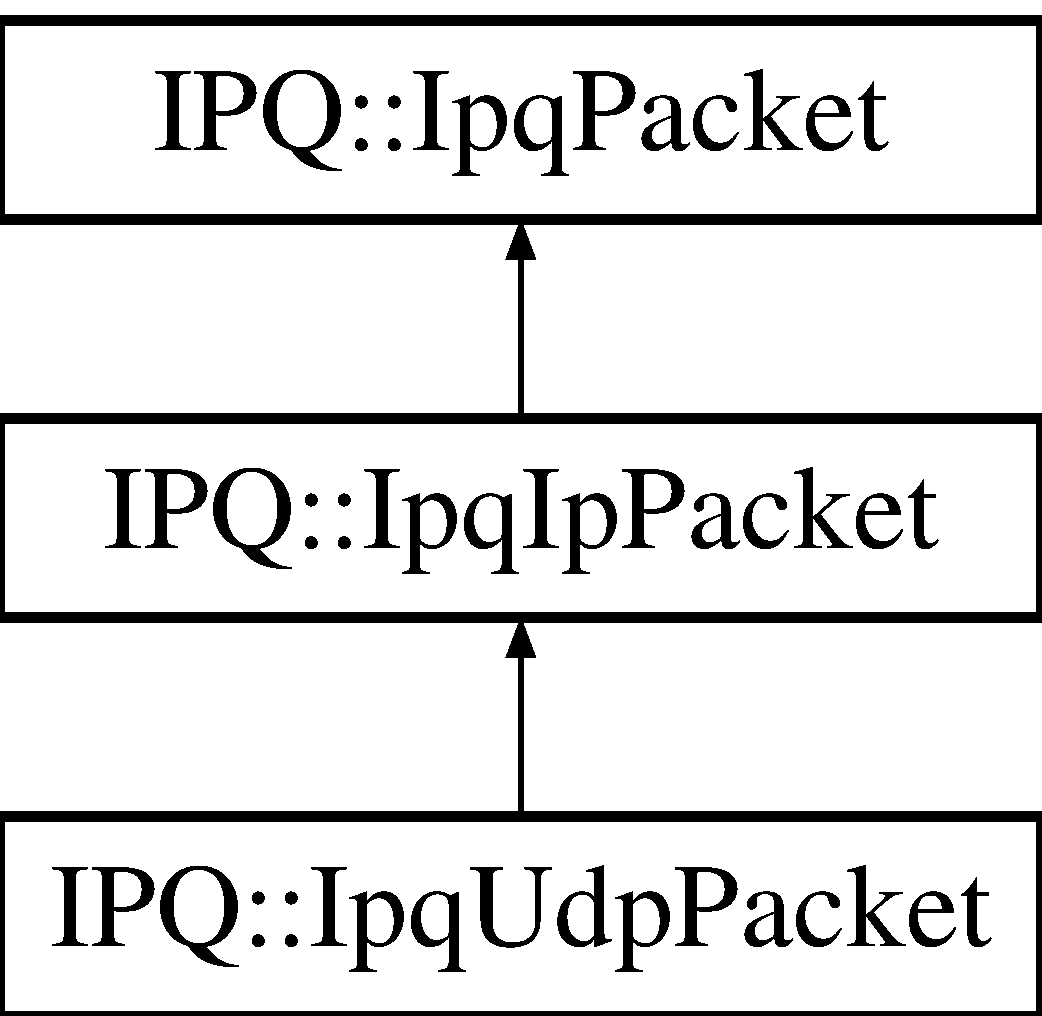
\includegraphics[height=3.000000cm]{classIPQ_1_1IpqUdpPacket}
\end{center}
\end{figure}
\subsection*{\-Public \-Member \-Functions}
\begin{DoxyCompactItemize}
\item 
in\-\_\-port\-\_\-t \hyperlink{classIPQ_1_1IpqUdpPacket_a4418916762f64f6996bd5cb1d7102c6e}{get\-Udp\-Source} () const 
\begin{DoxyCompactList}\small\item\em \-Retrieve the \-U\-D\-P source port of a packet. \end{DoxyCompactList}\item 
in\-\_\-port\-\_\-t \hyperlink{classIPQ_1_1IpqUdpPacket_aaf059aaa0d6027dd23e701c691ad07a7}{get\-Udp\-Dest} () const 
\begin{DoxyCompactList}\small\item\em \-Retrieve the \-U\-D\-P destination port of a packet. \end{DoxyCompactList}\item 
struct udphdr \& \hyperlink{classIPQ_1_1IpqUdpPacket_a88d136acc4488ec965f1d9d3acdc1c33}{get\-Udp\-Header} () const 
\begin{DoxyCompactList}\small\item\em \-Retrieve the complete \-U\-D\-P header of a packet. \end{DoxyCompactList}\item 
struct udphdr \& \hyperlink{classIPQ_1_1IpqUdpPacket_aeb63764de6bdb3a17f9c002414c4952b}{get\-Udp\-Header} ()
\begin{DoxyCompactList}\small\item\em \-Retrieve the complete \-U\-D\-P header of a packet. \end{DoxyCompactList}\item 
const boost\-::uint8\-\_\-t $\ast$ \hyperlink{classIPQ_1_1IpqUdpPacket_acfa3b21105ee5bc463d623e360bf492f}{get\-Udp\-Payload} (std\-::size\-\_\-t \&size) const 
\begin{DoxyCompactList}\small\item\em \-Retrive the \-U\-D\-P payload of a packet. \end{DoxyCompactList}\item 
boost\-::uint8\-\_\-t $\ast$ \hyperlink{classIPQ_1_1IpqUdpPacket_ac8751d02bda5f3f6e56fe990658cb4c7}{get\-Udp\-Payload} (std\-::size\-\_\-t \&size)
\begin{DoxyCompactList}\small\item\em \-Retrive the \-U\-D\-P payload of a packet. \end{DoxyCompactList}\item 
virtual void \hyperlink{classIPQ_1_1IpqUdpPacket_ad64646eb338bad97b6c593ad5225d36d}{print} (std\-::ostream \&out) const 
\begin{DoxyCompactList}\small\item\em \-Print a \-T\-C\-P packet to stdout in an easy-\/to-\/read format. \end{DoxyCompactList}\item 
virtual \hyperlink{classIPQ_1_1IpqUdpPacket_a8d59e6f50fc02dd78b97ab321de65de1}{$\sim$\-Ipq\-Udp\-Packet} ()
\begin{DoxyCompactList}\small\item\em \-Destructor for \hyperlink{classIPQ_1_1IpqUdpPacket}{\-Ipq\-Udp\-Packet}. \end{DoxyCompactList}\item 
in\-\_\-addr\-\_\-t \hyperlink{classIPQ_1_1IpqIpPacket_a4708c5a987eb9796566e2b3bdd072589}{get\-Ip\-Source} () const 
\begin{DoxyCompactList}\small\item\em \-Retrieve the source \-I\-P address of a packet. \end{DoxyCompactList}\item 
in\-\_\-addr\-\_\-t \hyperlink{classIPQ_1_1IpqIpPacket_a056bedcbf7998452d147f2d2ef68b611}{get\-Ip\-Dest} () const 
\begin{DoxyCompactList}\small\item\em \-Retrieve the destination \-I\-P address of a packet. \end{DoxyCompactList}\item 
boost\-::uint8\-\_\-t \hyperlink{classIPQ_1_1IpqIpPacket_aefa78bb7a89a337bb0c1d88c02d6d5cd}{get\-Protocol} () const 
\begin{DoxyCompactList}\small\item\em \-Retrieve the encapsulated protocol number of a packet. \end{DoxyCompactList}\item 
boost\-::uint16\-\_\-t \hyperlink{classIPQ_1_1IpqIpPacket_a937be4034dafdce171b7e90ae14f09d4}{get\-Id} () const 
\begin{DoxyCompactList}\small\item\em \-Retrieve the \-I\-P \-I\-D of a packet. \end{DoxyCompactList}\item 
boost\-::uint16\-\_\-t \hyperlink{classIPQ_1_1IpqIpPacket_a97e6e13ede2c6c6f028ee0eb1130600b}{get\-Frag\-Offset} () const 
\begin{DoxyCompactList}\small\item\em \-Retrieve the fragment offset of a packet, in bytes. \end{DoxyCompactList}\item 
bool \hyperlink{classIPQ_1_1IpqIpPacket_a76e0d09916fc816df3dab46cb29d479f}{get\-More\-Frags} () const 
\begin{DoxyCompactList}\small\item\em \-Retrieve the \char`\"{}more fragments to follow\char`\"{} flag of a packet. \end{DoxyCompactList}\item 
struct iphdr \& \hyperlink{classIPQ_1_1IpqIpPacket_abf46954191d96b4e2fe136f79ba6c8ac}{get\-Ip\-Header} () const 
\begin{DoxyCompactList}\small\item\em \-Retrieve the complete \-I\-P header of a packet. \end{DoxyCompactList}\item 
struct iphdr \& \hyperlink{classIPQ_1_1IpqIpPacket_aa6e89b7927e748d00b9562e85192b492}{get\-Ip\-Header} ()
\begin{DoxyCompactList}\small\item\em \-Retrieve the complete \-I\-P header of a packet. \end{DoxyCompactList}\item 
const boost\-::uint8\-\_\-t $\ast$ \hyperlink{classIPQ_1_1IpqIpPacket_adc020ff0aceeba0577e4bb90dcc6f86f}{get\-Ip\-Payload} (std\-::size\-\_\-t \&size) const 
\begin{DoxyCompactList}\small\item\em \-Retrive the \-I\-P payload of a packet. \end{DoxyCompactList}\item 
boost\-::uint8\-\_\-t $\ast$ \hyperlink{classIPQ_1_1IpqIpPacket_a47343dd1a4fc52c8fda6de4aa313a688}{get\-Ip\-Payload} (std\-::size\-\_\-t \&size)
\begin{DoxyCompactList}\small\item\em \-Retrive the \-I\-P payload of a packet. \end{DoxyCompactList}\item 
unsigned long \hyperlink{classIPQ_1_1IpqPacket_ac3cbbe2b61e12730ffe231fa19c96e5a}{get\-Nf\-Id} () const 
\begin{DoxyCompactList}\small\item\em \-Retrieve the \-Netfilter \-I\-D of a packet. \end{DoxyCompactList}\item 
unsigned long \hyperlink{classIPQ_1_1IpqPacket_ab97f0a4348e53cb69ed1da74e422dc78}{get\-Nf\-Mark} () const 
\begin{DoxyCompactList}\small\item\em \-Retrieve the \-Netfilter mark value of a packet. \end{DoxyCompactList}\item 
void \hyperlink{classIPQ_1_1IpqPacket_a430ce4f89e651724efdf56c9c1b1647e}{get\-Timestamp} (struct timeval \&time) const 
\begin{DoxyCompactList}\small\item\em \-Retrieve the arrival time of a packet. \end{DoxyCompactList}\item 
unsigned \hyperlink{classIPQ_1_1IpqPacket_ae13884fedce165702f4b71e0e4d93c0b}{get\-Nf\-Hook} () const 
\begin{DoxyCompactList}\small\item\em \-Retrieve the number of the \-Netfilter hook on which the packet arrived. \end{DoxyCompactList}\item 
const char(\& \hyperlink{classIPQ_1_1IpqPacket_a4cf04ca5da28410f27d87edefd679532}{get\-Indev\-Name} () const)\mbox{[}\-I\-F\-N\-A\-M\-S\-I\-Z\mbox{]}
\begin{DoxyCompactList}\small\item\em \-Retrieve the name of the interface on which the packet arrived, if available. \end{DoxyCompactList}\item 
const char(\& \hyperlink{classIPQ_1_1IpqPacket_a46dced8057de3bba7abfaaa63d7afcd4}{get\-Outdev\-Name} () const)\mbox{[}\-I\-F\-N\-A\-M\-S\-I\-Z\mbox{]}
\begin{DoxyCompactList}\small\item\em \-Retrieve the name of the interface on which the packet will leave, if available. \end{DoxyCompactList}\item 
unsigned short \hyperlink{classIPQ_1_1IpqPacket_ae150e294f043f4c699231a85d3b1ae0f}{get\-Hw\-Protocol} () const 
\begin{DoxyCompactList}\small\item\em \-Retrieve the hardware protocol number of the packet. \end{DoxyCompactList}\item 
unsigned short \hyperlink{classIPQ_1_1IpqPacket_ab6b76b146111c7ad11b96e87efe6634c}{get\-Hw\-Type} () const 
\begin{DoxyCompactList}\small\item\em \-Retrieve the hardware type on which the packet arrived. \end{DoxyCompactList}\item 
const unsigned char(\& \hyperlink{classIPQ_1_1IpqPacket_a8582ae732d6b66ca1f5201994159a84a}{get\-Hw\-Source} (unsigned short \&addrlen) const)\mbox{[}8\mbox{]}
\begin{DoxyCompactList}\small\item\em \-Retrieve the source hardware address of the packet. \end{DoxyCompactList}\item 
const boost\-::uint8\-\_\-t $\ast$ \hyperlink{classIPQ_1_1IpqPacket_a6dd7baeec66082658d882bff8862eb6c}{get\-Packet} (std\-::size\-\_\-t \&size) const 
\begin{DoxyCompactList}\small\item\em \-Retrieve the packet. \end{DoxyCompactList}\item 
boost\-::uint8\-\_\-t $\ast$ \hyperlink{classIPQ_1_1IpqPacket_a0bf3344a9eed5e2f6bc20890ffffe26e}{get\-Packet} (std\-::size\-\_\-t \&size)
\begin{DoxyCompactList}\small\item\em \-Retrieve the packet. \end{DoxyCompactList}\end{DoxyCompactItemize}
\subsection*{\-Protected \-Member \-Functions}
\begin{DoxyCompactItemize}
\item 
\hyperlink{classIPQ_1_1IpqUdpPacket_a2838137c87223b21b25be77950bc2d6e}{\-Ipq\-Udp\-Packet} (\hyperlink{classLibWheel_1_1auto__array}{\-Lib\-Wheel\-::auto\-\_\-array}$<$ boost\-::uint8\-\_\-t $>$ buf, std\-::size\-\_\-t buflen)
\begin{DoxyCompactList}\small\item\em \-Constructor for \hyperlink{classIPQ_1_1IpqTcpPacket}{\-Ipq\-Tcp\-Packet}. \end{DoxyCompactList}\item 
struct udphdr \& \hyperlink{classIPQ_1_1IpqUdpPacket_a0b0b2c8eb553e313cb439ef2ea13762d}{do\-Get\-Udp\-Header} () const 
\begin{DoxyCompactList}\small\item\em \-Retrieve the complete \-U\-D\-P header of a packet. \end{DoxyCompactList}\item 
boost\-::uint8\-\_\-t $\ast$ \hyperlink{classIPQ_1_1IpqUdpPacket_a1e789c47ce3f43b715969987edc6d06d}{do\-Get\-Udp\-Payload} (std\-::size\-\_\-t \&size) const 
\begin{DoxyCompactList}\small\item\em \-Retrive the \-U\-D\-P payload of a packet. \end{DoxyCompactList}\item 
virtual void \hyperlink{classIPQ_1_1IpqUdpPacket_abc390e2f22ffbd3d6d9a2df228cb71d6}{update\-Checksums} ()
\begin{DoxyCompactList}\small\item\em \-Update the checksums on an \-U\-D\-P packet. \end{DoxyCompactList}\item 
struct iphdr \& \hyperlink{classIPQ_1_1IpqIpPacket_a6be0afa1f616cbe7722ef817a65e24dc}{do\-Get\-Ip\-Header} () const 
\begin{DoxyCompactList}\small\item\em \-Retrieve the complete \-I\-P header of a packet. \end{DoxyCompactList}\item 
boost\-::uint8\-\_\-t $\ast$ \hyperlink{classIPQ_1_1IpqIpPacket_ab78709e0712a1912d19114f815407303}{do\-Get\-Ip\-Payload} (std\-::size\-\_\-t \&size) const 
\begin{DoxyCompactList}\small\item\em \-Retrive the \-I\-P payload of a packet. \end{DoxyCompactList}\item 
boost\-::uint8\-\_\-t $\ast$ \hyperlink{classIPQ_1_1IpqPacket_a7b8f489a9cec36058eaee43f6566a999}{do\-Get\-Packet} (std\-::size\-\_\-t \&size) const 
\begin{DoxyCompactList}\small\item\em \-Retrieve the packet. \end{DoxyCompactList}\end{DoxyCompactItemize}
\subsection*{\-Static \-Protected \-Member \-Functions}
\begin{DoxyCompactItemize}
\item 
static \hyperlink{classIPQ_1_1IpqPacket}{\-Ipq\-Packet} $\ast$ \hyperlink{classIPQ_1_1IpqPacket_adf6099052730113814e9fe7312ec7b8c}{create\-Packet} (\hyperlink{classLibWheel_1_1auto__array}{\-Lib\-Wheel\-::auto\-\_\-array}$<$ boost\-::uint8\-\_\-t $>$ buf, std\-::size\-\_\-t buflen)
\begin{DoxyCompactList}\small\item\em \-Create an \hyperlink{classIPQ_1_1IpqPacket}{\-Ipq\-Packet} or one of its subclasses from a libipq packet message. \end{DoxyCompactList}\end{DoxyCompactItemize}
\subsection*{\-Protected \-Attributes}
\begin{DoxyCompactItemize}
\item 
\hyperlink{classLibWheel_1_1auto__array}{\-Lib\-Wheel\-::auto\-\_\-array}\*
$<$ boost\-::uint8\-\_\-t $>$ \hyperlink{classIPQ_1_1IpqPacket_a2bdf247f13a3e9f86e9e3846e6a9cb45}{packet}
\begin{DoxyCompactList}\small\item\em \-The packet message received from kernelspace. \end{DoxyCompactList}\item 
std\-::size\-\_\-t \hyperlink{classIPQ_1_1IpqPacket_a9b448a070c5ae499e32d2af5a190b86d}{packet\-Len}
\begin{DoxyCompactList}\small\item\em the length of the packet message in \hyperlink{classIPQ_1_1IpqPacket_a2bdf247f13a3e9f86e9e3846e6a9cb45}{\-Ipq\-Packet\-::packet}, in bytes. \end{DoxyCompactList}\item 
bool \hyperlink{classIPQ_1_1IpqPacket_a00acebf51531043a8536f20bb9412d61}{dirty}
\begin{DoxyCompactList}\small\item\em {\bfseries true} if the packet has been modified but checksums have not been updated; {\bfseries false} otherwise. \end{DoxyCompactList}\end{DoxyCompactItemize}
\subsection*{\-Friends}
\begin{DoxyCompactItemize}
\item 
\hyperlink{classIPQ_1_1IpqPacket}{\-Ipq\-Packet} $\ast$ \hyperlink{classIPQ_1_1IpqUdpPacket_af2019ef9442b13f8da0f53a082a9b308}{\-Ipq\-Packet\-::create\-Packet} (\hyperlink{classLibWheel_1_1auto__array}{\-Lib\-Wheel\-::auto\-\_\-array}$<$ boost\-::uint8\-\_\-t $>$, std\-::size\-\_\-t)
\begin{DoxyCompactList}\small\item\em \-Allow \-Ipq\-Socket\-::create\-Packet() to access the contstructor. \end{DoxyCompactList}\end{DoxyCompactItemize}


\subsection{\-Detailed \-Description}
\-An complete \-I\-Pv4/\-U\-D\-P packet that was received via \hyperlink{classIPQ_1_1IpqSocket}{\-Ipq\-Socket}. 

\-Contains \-U\-D\-P header fields and the \-U\-D\-P payload. 

\subsection{\-Constructor \& \-Destructor \-Documentation}
\hypertarget{classIPQ_1_1IpqUdpPacket_a8d59e6f50fc02dd78b97ab321de65de1}{
\index{\-I\-P\-Q\-::\-Ipq\-Udp\-Packet@{\-I\-P\-Q\-::\-Ipq\-Udp\-Packet}!$\sim$\-Ipq\-Udp\-Packet@{$\sim$\-Ipq\-Udp\-Packet}}
\index{$\sim$\-Ipq\-Udp\-Packet@{$\sim$\-Ipq\-Udp\-Packet}!IPQ::IpqUdpPacket@{\-I\-P\-Q\-::\-Ipq\-Udp\-Packet}}
\subsubsection[{$\sim$\-Ipq\-Udp\-Packet}]{\setlength{\rightskip}{0pt plus 5cm}\-I\-P\-Q\-::\-Ipq\-Udp\-Packet\-::$\sim$\-Ipq\-Udp\-Packet (
\begin{DoxyParamCaption}
{}
\end{DoxyParamCaption}
)\hspace{0.3cm}{\ttfamily  \mbox{[}virtual\mbox{]}}}}
\label{classIPQ_1_1IpqUdpPacket_a8d59e6f50fc02dd78b97ab321de65de1}


\-Destructor for \hyperlink{classIPQ_1_1IpqUdpPacket}{\-Ipq\-Udp\-Packet}. 



\-Definition at line 1314 of file \-I\-P\-Q.\-cpp.

\hypertarget{classIPQ_1_1IpqUdpPacket_a2838137c87223b21b25be77950bc2d6e}{
\index{\-I\-P\-Q\-::\-Ipq\-Udp\-Packet@{\-I\-P\-Q\-::\-Ipq\-Udp\-Packet}!\-Ipq\-Udp\-Packet@{\-Ipq\-Udp\-Packet}}
\index{\-Ipq\-Udp\-Packet@{\-Ipq\-Udp\-Packet}!IPQ::IpqUdpPacket@{\-I\-P\-Q\-::\-Ipq\-Udp\-Packet}}
\subsubsection[{\-Ipq\-Udp\-Packet}]{\setlength{\rightskip}{0pt plus 5cm}\-I\-P\-Q\-::\-Ipq\-Udp\-Packet\-::\-Ipq\-Udp\-Packet (
\begin{DoxyParamCaption}
\item[{{\bf \-Lib\-Wheel\-::auto\-\_\-array}$<$ boost\-::uint8\-\_\-t $>$}]{buf, }
\item[{std\-::size\-\_\-t}]{buflen}
\end{DoxyParamCaption}
)\hspace{0.3cm}{\ttfamily  \mbox{[}protected\mbox{]}}}}
\label{classIPQ_1_1IpqUdpPacket_a2838137c87223b21b25be77950bc2d6e}


\-Constructor for \hyperlink{classIPQ_1_1IpqTcpPacket}{\-Ipq\-Tcp\-Packet}. 

\-Initializes an \hyperlink{classIPQ_1_1IpqTcpPacket}{\-Ipq\-Tcp\-Packet} from a libipq packet message. 

\-Definition at line 1322 of file \-I\-P\-Q.\-cpp.



\subsection{\-Member \-Function \-Documentation}
\hypertarget{classIPQ_1_1IpqPacket_adf6099052730113814e9fe7312ec7b8c}{
\index{\-I\-P\-Q\-::\-Ipq\-Udp\-Packet@{\-I\-P\-Q\-::\-Ipq\-Udp\-Packet}!create\-Packet@{create\-Packet}}
\index{create\-Packet@{create\-Packet}!IPQ::IpqUdpPacket@{\-I\-P\-Q\-::\-Ipq\-Udp\-Packet}}
\subsubsection[{create\-Packet}]{\setlength{\rightskip}{0pt plus 5cm}{\bf \-Ipq\-Packet} $\ast$ \-I\-P\-Q\-::\-Ipq\-Packet\-::create\-Packet (
\begin{DoxyParamCaption}
\item[{{\bf \-Lib\-Wheel\-::auto\-\_\-array}$<$ boost\-::uint8\-\_\-t $>$}]{buf, }
\item[{std\-::size\-\_\-t}]{buflen}
\end{DoxyParamCaption}
)\hspace{0.3cm}{\ttfamily  \mbox{[}static, protected, inherited\mbox{]}}}}
\label{classIPQ_1_1IpqPacket_adf6099052730113814e9fe7312ec7b8c}


\-Create an \hyperlink{classIPQ_1_1IpqPacket}{\-Ipq\-Packet} or one of its subclasses from a libipq packet message. 

\-A packet will be deemed to be an \-I\-Pv4 packet if it has a full \-I\-Pv4 header and the data length indicated by the header matches the packet's length. \-A packet will be deemed to be a \-T\-C\-P or \-U\-D\-P packet if it is an \-I\-Pv4 packet and it has a full \-T\-C\-P or \-U\-D\-P header. \begin{DoxyReturn}{\-Returns}
\-A pointer to a dynamically-\/allocated \hyperlink{classIPQ_1_1IpqPacket}{\-Ipq\-Packet}, or one of its subclasses. \-This pointer must be freed using {\bfseries delete}, and a verdict should be set on it using \hyperlink{classIPQ_1_1IpqSocket_a53e0f4e45363cbcd919a2d96ee7cf0a8}{\-Ipq\-Socket\-::send\-Response()}. 
\end{DoxyReturn}


\-Definition at line 731 of file \-I\-P\-Q.\-cpp.



\-References \-Lib\-Wheel\-::auto\-\_\-array\-::get(), and \-I\-P\-Q\-::\-Ipq\-Packet\-::\-Ipq\-Packet().



\-Referenced by \-I\-P\-Q\-::\-Ipq\-Socket\-::recv\-Packet().

\hypertarget{classIPQ_1_1IpqIpPacket_a6be0afa1f616cbe7722ef817a65e24dc}{
\index{\-I\-P\-Q\-::\-Ipq\-Udp\-Packet@{\-I\-P\-Q\-::\-Ipq\-Udp\-Packet}!do\-Get\-Ip\-Header@{do\-Get\-Ip\-Header}}
\index{do\-Get\-Ip\-Header@{do\-Get\-Ip\-Header}!IPQ::IpqUdpPacket@{\-I\-P\-Q\-::\-Ipq\-Udp\-Packet}}
\subsubsection[{do\-Get\-Ip\-Header}]{\setlength{\rightskip}{0pt plus 5cm}struct iphdr \& \-I\-P\-Q\-::\-Ipq\-Ip\-Packet\-::do\-Get\-Ip\-Header (
\begin{DoxyParamCaption}
{}
\end{DoxyParamCaption}
) const\hspace{0.3cm}{\ttfamily  \mbox{[}read, protected, inherited\mbox{]}}}}
\label{classIPQ_1_1IpqIpPacket_a6be0afa1f616cbe7722ef817a65e24dc}


\-Retrieve the complete \-I\-P header of a packet. 

\-A reference to the packet's \-I\-P header. 

\-Definition at line 928 of file \-I\-P\-Q.\-cpp.



\-References \-I\-P\-Q\-::\-Ipq\-Packet\-::packet, and \-Lib\-Wheel\-::auto\-\_\-array\-::get().



\-Referenced by \-I\-P\-Q\-::\-Ipq\-Ip\-Packet\-::get\-Ip\-Header().

\hypertarget{classIPQ_1_1IpqIpPacket_ab78709e0712a1912d19114f815407303}{
\index{\-I\-P\-Q\-::\-Ipq\-Udp\-Packet@{\-I\-P\-Q\-::\-Ipq\-Udp\-Packet}!do\-Get\-Ip\-Payload@{do\-Get\-Ip\-Payload}}
\index{do\-Get\-Ip\-Payload@{do\-Get\-Ip\-Payload}!IPQ::IpqUdpPacket@{\-I\-P\-Q\-::\-Ipq\-Udp\-Packet}}
\subsubsection[{do\-Get\-Ip\-Payload}]{\setlength{\rightskip}{0pt plus 5cm}boost\-::uint8\-\_\-t $\ast$ \-I\-P\-Q\-::\-Ipq\-Ip\-Packet\-::do\-Get\-Ip\-Payload (
\begin{DoxyParamCaption}
\item[{std\-::size\-\_\-t \&}]{size}
\end{DoxyParamCaption}
) const\hspace{0.3cm}{\ttfamily  \mbox{[}protected, inherited\mbox{]}}}}
\label{classIPQ_1_1IpqIpPacket_ab78709e0712a1912d19114f815407303}


\-Retrive the \-I\-P payload of a packet. 


\begin{DoxyParams}[1]{\-Parameters}
\mbox{\tt out}  & {\em size} & \-A reference to a location to store the packet's \-I\-P payload size, in bytes.. \\
\hline
\end{DoxyParams}
\begin{DoxyReturn}{\-Returns}
\-A const pointer to the packet's \-I\-P payload. 
\end{DoxyReturn}


\-Definition at line 941 of file \-I\-P\-Q.\-cpp.



\-References \-I\-P\-Q\-::\-Ipq\-Packet\-::packet, and \-Lib\-Wheel\-::auto\-\_\-array\-::get().



\-Referenced by \-I\-P\-Q\-::\-Ipq\-Ip\-Packet\-::get\-Ip\-Payload().

\hypertarget{classIPQ_1_1IpqPacket_a7b8f489a9cec36058eaee43f6566a999}{
\index{\-I\-P\-Q\-::\-Ipq\-Udp\-Packet@{\-I\-P\-Q\-::\-Ipq\-Udp\-Packet}!do\-Get\-Packet@{do\-Get\-Packet}}
\index{do\-Get\-Packet@{do\-Get\-Packet}!IPQ::IpqUdpPacket@{\-I\-P\-Q\-::\-Ipq\-Udp\-Packet}}
\subsubsection[{do\-Get\-Packet}]{\setlength{\rightskip}{0pt plus 5cm}boost\-::uint8\-\_\-t $\ast$ \-I\-P\-Q\-::\-Ipq\-Packet\-::do\-Get\-Packet (
\begin{DoxyParamCaption}
\item[{std\-::size\-\_\-t \&}]{size}
\end{DoxyParamCaption}
) const\hspace{0.3cm}{\ttfamily  \mbox{[}protected, inherited\mbox{]}}}}
\label{classIPQ_1_1IpqPacket_a7b8f489a9cec36058eaee43f6566a999}


\-Retrieve the packet. 

\-It will only be available if the copy mode on the libipq handle used to receive it was \hyperlink{classIPQ_1_1IpqSocket_afee6d75480079906ecf6544f8467e0ccafc1e90369658a807b2c970d3e15b01d4}{\-Ipq\-Socket\-::\-P\-A\-C\-K\-E\-T} and the copy range was greater than zero. 
\begin{DoxyParams}[1]{\-Parameters}
\mbox{\tt out}  & {\em size} & \-A reference to a location to write the length of the payload, in bytes. \\
\hline
\end{DoxyParams}
\begin{DoxyReturn}{\-Returns}
\-A pointer to the packet. 
\end{DoxyReturn}


\-Definition at line 703 of file \-I\-P\-Q.\-cpp.



\-References \-I\-P\-Q\-::\-Ipq\-Packet\-::packet, and \-Lib\-Wheel\-::auto\-\_\-array\-::get().



\-Referenced by \-I\-P\-Q\-::\-Ipq\-Packet\-::get\-Packet().

\hypertarget{classIPQ_1_1IpqUdpPacket_a0b0b2c8eb553e313cb439ef2ea13762d}{
\index{\-I\-P\-Q\-::\-Ipq\-Udp\-Packet@{\-I\-P\-Q\-::\-Ipq\-Udp\-Packet}!do\-Get\-Udp\-Header@{do\-Get\-Udp\-Header}}
\index{do\-Get\-Udp\-Header@{do\-Get\-Udp\-Header}!IPQ::IpqUdpPacket@{\-I\-P\-Q\-::\-Ipq\-Udp\-Packet}}
\subsubsection[{do\-Get\-Udp\-Header}]{\setlength{\rightskip}{0pt plus 5cm}struct udphdr \& \-I\-P\-Q\-::\-Ipq\-Udp\-Packet\-::do\-Get\-Udp\-Header (
\begin{DoxyParamCaption}
{}
\end{DoxyParamCaption}
) const\hspace{0.3cm}{\ttfamily  \mbox{[}read, protected\mbox{]}}}}
\label{classIPQ_1_1IpqUdpPacket_a0b0b2c8eb553e313cb439ef2ea13762d}


\-Retrieve the complete \-U\-D\-P header of a packet. 

\-A reference to the packet's \-U\-D\-P header. 

\-Definition at line 1332 of file \-I\-P\-Q.\-cpp.



\-References \-I\-P\-Q\-::\-Ipq\-Packet\-::packet, and \-Lib\-Wheel\-::auto\-\_\-array\-::get().



\-Referenced by get\-Udp\-Header().

\hypertarget{classIPQ_1_1IpqUdpPacket_a1e789c47ce3f43b715969987edc6d06d}{
\index{\-I\-P\-Q\-::\-Ipq\-Udp\-Packet@{\-I\-P\-Q\-::\-Ipq\-Udp\-Packet}!do\-Get\-Udp\-Payload@{do\-Get\-Udp\-Payload}}
\index{do\-Get\-Udp\-Payload@{do\-Get\-Udp\-Payload}!IPQ::IpqUdpPacket@{\-I\-P\-Q\-::\-Ipq\-Udp\-Packet}}
\subsubsection[{do\-Get\-Udp\-Payload}]{\setlength{\rightskip}{0pt plus 5cm}boost\-::uint8\-\_\-t $\ast$ \-I\-P\-Q\-::\-Ipq\-Udp\-Packet\-::do\-Get\-Udp\-Payload (
\begin{DoxyParamCaption}
\item[{std\-::size\-\_\-t \&}]{size}
\end{DoxyParamCaption}
) const\hspace{0.3cm}{\ttfamily  \mbox{[}protected\mbox{]}}}}
\label{classIPQ_1_1IpqUdpPacket_a1e789c47ce3f43b715969987edc6d06d}


\-Retrive the \-U\-D\-P payload of a packet. 


\begin{DoxyParams}[1]{\-Parameters}
\mbox{\tt out}  & {\em size} & \-A reference to a location to store the packet's \-U\-D\-P payload size, in bytes.. \\
\hline
\end{DoxyParams}
\begin{DoxyReturn}{\-Returns}
\-A pointer to the packet's \-U\-D\-P payload. 
\end{DoxyReturn}


\-Definition at line 1346 of file \-I\-P\-Q.\-cpp.



\-References \-I\-P\-Q\-::\-Ipq\-Packet\-::packet, and \-Lib\-Wheel\-::auto\-\_\-array\-::get().



\-Referenced by get\-Udp\-Payload().

\hypertarget{classIPQ_1_1IpqIpPacket_a97e6e13ede2c6c6f028ee0eb1130600b}{
\index{\-I\-P\-Q\-::\-Ipq\-Udp\-Packet@{\-I\-P\-Q\-::\-Ipq\-Udp\-Packet}!get\-Frag\-Offset@{get\-Frag\-Offset}}
\index{get\-Frag\-Offset@{get\-Frag\-Offset}!IPQ::IpqUdpPacket@{\-I\-P\-Q\-::\-Ipq\-Udp\-Packet}}
\subsubsection[{get\-Frag\-Offset}]{\setlength{\rightskip}{0pt plus 5cm}boost\-::uint16\-\_\-t \-I\-P\-Q\-::\-Ipq\-Ip\-Packet\-::get\-Frag\-Offset (
\begin{DoxyParamCaption}
{}
\end{DoxyParamCaption}
) const\hspace{0.3cm}{\ttfamily  \mbox{[}inherited\mbox{]}}}}
\label{classIPQ_1_1IpqIpPacket_a97e6e13ede2c6c6f028ee0eb1130600b}


\-Retrieve the fragment offset of a packet, in bytes. 

\-If not zero, then this is a non-\/leading fragment. \begin{DoxyReturn}{\-Returns}
\-The packet's fragment offset. 
\end{DoxyReturn}


\-Definition at line 817 of file \-I\-P\-Q.\-cpp.



\-References \-I\-P\-Q\-::\-Ipq\-Ip\-Packet\-::get\-Ip\-Header().



\-Referenced by \-I\-P\-Q\-::\-Ipq\-Ip\-Packet\-::print(), and \-N\-E\-R\-D\-::\-Connection\-Server\-::handle\-Packet().

\hypertarget{classIPQ_1_1IpqPacket_ae150e294f043f4c699231a85d3b1ae0f}{
\index{\-I\-P\-Q\-::\-Ipq\-Udp\-Packet@{\-I\-P\-Q\-::\-Ipq\-Udp\-Packet}!get\-Hw\-Protocol@{get\-Hw\-Protocol}}
\index{get\-Hw\-Protocol@{get\-Hw\-Protocol}!IPQ::IpqUdpPacket@{\-I\-P\-Q\-::\-Ipq\-Udp\-Packet}}
\subsubsection[{get\-Hw\-Protocol}]{\setlength{\rightskip}{0pt plus 5cm}unsigned short \-I\-P\-Q\-::\-Ipq\-Packet\-::get\-Hw\-Protocol (
\begin{DoxyParamCaption}
{}
\end{DoxyParamCaption}
) const\hspace{0.3cm}{\ttfamily  \mbox{[}inherited\mbox{]}}}}
\label{classIPQ_1_1IpqPacket_ae150e294f043f4c699231a85d3b1ae0f}


\-Retrieve the hardware protocol number of the packet. 

\begin{DoxyReturn}{\-Returns}
\-The packet's hardware protocol number. 
\end{DoxyReturn}


\-Definition at line 585 of file \-I\-P\-Q.\-cpp.



\-References \-I\-P\-Q\-::\-Ipq\-Packet\-::packet, and \-Lib\-Wheel\-::auto\-\_\-array\-::get().



\-Referenced by \-I\-P\-Q\-::\-Ipq\-Packet\-::print().

\hypertarget{classIPQ_1_1IpqPacket_a8582ae732d6b66ca1f5201994159a84a}{
\index{\-I\-P\-Q\-::\-Ipq\-Udp\-Packet@{\-I\-P\-Q\-::\-Ipq\-Udp\-Packet}!get\-Hw\-Source@{get\-Hw\-Source}}
\index{get\-Hw\-Source@{get\-Hw\-Source}!IPQ::IpqUdpPacket@{\-I\-P\-Q\-::\-Ipq\-Udp\-Packet}}
\subsubsection[{get\-Hw\-Source}]{\setlength{\rightskip}{0pt plus 5cm}const unsigned char(\& \-I\-P\-Q\-::\-Ipq\-Packet\-::get\-Hw\-Source (
\begin{DoxyParamCaption}
\item[{unsigned short \&}]{addrlen}
\end{DoxyParamCaption}
))\mbox{[}8\mbox{]}\hspace{0.3cm}{\ttfamily  \mbox{[}inherited\mbox{]}}}}
\label{classIPQ_1_1IpqPacket_a8582ae732d6b66ca1f5201994159a84a}


\-Retrieve the source hardware address of the packet. 


\begin{DoxyParams}[1]{\-Parameters}
\mbox{\tt out}  & {\em addrlen} & \-A reference to a location to write the actual length of the address, in bytes. \\
\hline
\end{DoxyParams}
\begin{DoxyReturn}{\-Returns}
\-A reference to the packet's source hardware address. 
\end{DoxyReturn}


\-Definition at line 608 of file \-I\-P\-Q.\-cpp.



\-Referenced by \-I\-P\-Q\-::\-Ipq\-Packet\-::print().

\hypertarget{classIPQ_1_1IpqPacket_ab6b76b146111c7ad11b96e87efe6634c}{
\index{\-I\-P\-Q\-::\-Ipq\-Udp\-Packet@{\-I\-P\-Q\-::\-Ipq\-Udp\-Packet}!get\-Hw\-Type@{get\-Hw\-Type}}
\index{get\-Hw\-Type@{get\-Hw\-Type}!IPQ::IpqUdpPacket@{\-I\-P\-Q\-::\-Ipq\-Udp\-Packet}}
\subsubsection[{get\-Hw\-Type}]{\setlength{\rightskip}{0pt plus 5cm}unsigned short \-I\-P\-Q\-::\-Ipq\-Packet\-::get\-Hw\-Type (
\begin{DoxyParamCaption}
{}
\end{DoxyParamCaption}
) const\hspace{0.3cm}{\ttfamily  \mbox{[}inherited\mbox{]}}}}
\label{classIPQ_1_1IpqPacket_ab6b76b146111c7ad11b96e87efe6634c}


\-Retrieve the hardware type on which the packet arrived. 

\begin{DoxyReturn}{\-Returns}
\-The packet's arrival hardware type. 
\end{DoxyReturn}


\-Definition at line 596 of file \-I\-P\-Q.\-cpp.



\-References \-I\-P\-Q\-::\-Ipq\-Packet\-::packet, and \-Lib\-Wheel\-::auto\-\_\-array\-::get().



\-Referenced by \-I\-P\-Q\-::\-Ipq\-Packet\-::print().

\hypertarget{classIPQ_1_1IpqIpPacket_a937be4034dafdce171b7e90ae14f09d4}{
\index{\-I\-P\-Q\-::\-Ipq\-Udp\-Packet@{\-I\-P\-Q\-::\-Ipq\-Udp\-Packet}!get\-Id@{get\-Id}}
\index{get\-Id@{get\-Id}!IPQ::IpqUdpPacket@{\-I\-P\-Q\-::\-Ipq\-Udp\-Packet}}
\subsubsection[{get\-Id}]{\setlength{\rightskip}{0pt plus 5cm}boost\-::uint16\-\_\-t \-I\-P\-Q\-::\-Ipq\-Ip\-Packet\-::get\-Id (
\begin{DoxyParamCaption}
{}
\end{DoxyParamCaption}
) const\hspace{0.3cm}{\ttfamily  \mbox{[}inherited\mbox{]}}}}
\label{classIPQ_1_1IpqIpPacket_a937be4034dafdce171b7e90ae14f09d4}


\-Retrieve the \-I\-P \-I\-D of a packet. 

\begin{DoxyReturn}{\-Returns}
\-The packet's \-I\-P\-I\-D. 
\end{DoxyReturn}


\-Definition at line 805 of file \-I\-P\-Q.\-cpp.



\-References \-I\-P\-Q\-::\-Ipq\-Ip\-Packet\-::get\-Ip\-Header().



\-Referenced by \-I\-P\-Q\-::\-Ipq\-Ip\-Packet\-::print().

\hypertarget{classIPQ_1_1IpqPacket_a4cf04ca5da28410f27d87edefd679532}{
\index{\-I\-P\-Q\-::\-Ipq\-Udp\-Packet@{\-I\-P\-Q\-::\-Ipq\-Udp\-Packet}!get\-Indev\-Name@{get\-Indev\-Name}}
\index{get\-Indev\-Name@{get\-Indev\-Name}!IPQ::IpqUdpPacket@{\-I\-P\-Q\-::\-Ipq\-Udp\-Packet}}
\subsubsection[{get\-Indev\-Name}]{\setlength{\rightskip}{0pt plus 5cm}const char(\& \-I\-P\-Q\-::\-Ipq\-Packet\-::get\-Indev\-Name (
\begin{DoxyParamCaption}
{}
\end{DoxyParamCaption}
))\mbox{[}\-I\-F\-N\-A\-M\-S\-I\-Z\mbox{]}\hspace{0.3cm}{\ttfamily  \mbox{[}inherited\mbox{]}}}}
\label{classIPQ_1_1IpqPacket_a4cf04ca5da28410f27d87edefd679532}


\-Retrieve the name of the interface on which the packet arrived, if available. 

\begin{DoxyReturn}{\-Returns}
\-A reference to the packet's arrival interface name. 
\end{DoxyReturn}


\-Definition at line 563 of file \-I\-P\-Q.\-cpp.



\-Referenced by \-I\-P\-Q\-::\-Ipq\-Packet\-::print().

\hypertarget{classIPQ_1_1IpqIpPacket_a056bedcbf7998452d147f2d2ef68b611}{
\index{\-I\-P\-Q\-::\-Ipq\-Udp\-Packet@{\-I\-P\-Q\-::\-Ipq\-Udp\-Packet}!get\-Ip\-Dest@{get\-Ip\-Dest}}
\index{get\-Ip\-Dest@{get\-Ip\-Dest}!IPQ::IpqUdpPacket@{\-I\-P\-Q\-::\-Ipq\-Udp\-Packet}}
\subsubsection[{get\-Ip\-Dest}]{\setlength{\rightskip}{0pt plus 5cm}in\-\_\-addr\-\_\-t \-I\-P\-Q\-::\-Ipq\-Ip\-Packet\-::get\-Ip\-Dest (
\begin{DoxyParamCaption}
{}
\end{DoxyParamCaption}
) const\hspace{0.3cm}{\ttfamily  \mbox{[}inherited\mbox{]}}}}
\label{classIPQ_1_1IpqIpPacket_a056bedcbf7998452d147f2d2ef68b611}


\-Retrieve the destination \-I\-P address of a packet. 

\begin{DoxyReturn}{\-Returns}
\-The packet's destination \-I\-P address. 
\end{DoxyReturn}


\-Definition at line 783 of file \-I\-P\-Q.\-cpp.



\-References \-I\-P\-Q\-::\-Ipq\-Ip\-Packet\-::get\-Ip\-Header().



\-Referenced by \-I\-P\-Q\-::\-Ipq\-Socket\-::send\-Response(), \-I\-P\-Q\-::\-Ipq\-Ip\-Packet\-::print(), \-N\-E\-R\-D\-::\-Connection\-Server\-::handle\-Packet(), and \-N\-E\-R\-D\-::\-Connection\-Server\-::create\-Connection().

\hypertarget{classIPQ_1_1IpqIpPacket_abf46954191d96b4e2fe136f79ba6c8ac}{
\index{\-I\-P\-Q\-::\-Ipq\-Udp\-Packet@{\-I\-P\-Q\-::\-Ipq\-Udp\-Packet}!get\-Ip\-Header@{get\-Ip\-Header}}
\index{get\-Ip\-Header@{get\-Ip\-Header}!IPQ::IpqUdpPacket@{\-I\-P\-Q\-::\-Ipq\-Udp\-Packet}}
\subsubsection[{get\-Ip\-Header}]{\setlength{\rightskip}{0pt plus 5cm}struct iphdr \& \-I\-P\-Q\-::\-Ipq\-Ip\-Packet\-::get\-Ip\-Header (
\begin{DoxyParamCaption}
{}
\end{DoxyParamCaption}
) const\hspace{0.3cm}{\ttfamily  \mbox{[}read, inherited\mbox{]}}}}
\label{classIPQ_1_1IpqIpPacket_abf46954191d96b4e2fe136f79ba6c8ac}


\-Retrieve the complete \-I\-P header of a packet. 

\-A const reference to the packet's \-I\-P header. 

\-Definition at line 840 of file \-I\-P\-Q.\-cpp.



\-References \-I\-P\-Q\-::\-Ipq\-Ip\-Packet\-::do\-Get\-Ip\-Header().



\-Referenced by \-I\-P\-Q\-::\-Ipq\-Ip\-Packet\-::get\-Ip\-Source(), \-I\-P\-Q\-::\-Ipq\-Ip\-Packet\-::get\-Ip\-Dest(), \-I\-P\-Q\-::\-Ipq\-Ip\-Packet\-::get\-Protocol(), \-I\-P\-Q\-::\-Ipq\-Ip\-Packet\-::get\-Id(), \-I\-P\-Q\-::\-Ipq\-Ip\-Packet\-::get\-Frag\-Offset(), \-I\-P\-Q\-::\-Ipq\-Ip\-Packet\-::get\-More\-Frags(), \-I\-P\-Q\-::\-Ipq\-Ip\-Packet\-::update\-Checksums(), \-I\-P\-Q\-::\-Ipq\-Tcp\-Packet\-::update\-Checksums(), update\-Checksums(), and \-N\-E\-R\-D\-::\-Connection\-Server\-::handle\-Packet().

\hypertarget{classIPQ_1_1IpqIpPacket_aa6e89b7927e748d00b9562e85192b492}{
\index{\-I\-P\-Q\-::\-Ipq\-Udp\-Packet@{\-I\-P\-Q\-::\-Ipq\-Udp\-Packet}!get\-Ip\-Header@{get\-Ip\-Header}}
\index{get\-Ip\-Header@{get\-Ip\-Header}!IPQ::IpqUdpPacket@{\-I\-P\-Q\-::\-Ipq\-Udp\-Packet}}
\subsubsection[{get\-Ip\-Header}]{\setlength{\rightskip}{0pt plus 5cm}struct iphdr \& \-I\-P\-Q\-::\-Ipq\-Ip\-Packet\-::get\-Ip\-Header (
\begin{DoxyParamCaption}
{}
\end{DoxyParamCaption}
)\hspace{0.3cm}{\ttfamily  \mbox{[}read, inherited\mbox{]}}}}
\label{classIPQ_1_1IpqIpPacket_aa6e89b7927e748d00b9562e85192b492}


\-Retrieve the complete \-I\-P header of a packet. 

\-A reference to the packet's \-I\-P header. \begin{DoxyNote}{\-Note}
\-This method sets the packet's dirty flag, requiring that the packet's checksums be recomputed before a verdict is set. 
\end{DoxyNote}


\-Definition at line 853 of file \-I\-P\-Q.\-cpp.



\-References \-I\-P\-Q\-::\-Ipq\-Packet\-::dirty, and \-I\-P\-Q\-::\-Ipq\-Ip\-Packet\-::do\-Get\-Ip\-Header().

\hypertarget{classIPQ_1_1IpqIpPacket_adc020ff0aceeba0577e4bb90dcc6f86f}{
\index{\-I\-P\-Q\-::\-Ipq\-Udp\-Packet@{\-I\-P\-Q\-::\-Ipq\-Udp\-Packet}!get\-Ip\-Payload@{get\-Ip\-Payload}}
\index{get\-Ip\-Payload@{get\-Ip\-Payload}!IPQ::IpqUdpPacket@{\-I\-P\-Q\-::\-Ipq\-Udp\-Packet}}
\subsubsection[{get\-Ip\-Payload}]{\setlength{\rightskip}{0pt plus 5cm}const boost\-::uint8\-\_\-t $\ast$ \-I\-P\-Q\-::\-Ipq\-Ip\-Packet\-::get\-Ip\-Payload (
\begin{DoxyParamCaption}
\item[{std\-::size\-\_\-t \&}]{size}
\end{DoxyParamCaption}
) const\hspace{0.3cm}{\ttfamily  \mbox{[}inherited\mbox{]}}}}
\label{classIPQ_1_1IpqIpPacket_adc020ff0aceeba0577e4bb90dcc6f86f}


\-Retrive the \-I\-P payload of a packet. 


\begin{DoxyParams}[1]{\-Parameters}
\mbox{\tt out}  & {\em size} & \-A reference to a location to store the packet's \-I\-P payload size, in bytes.. \\
\hline
\end{DoxyParams}
\begin{DoxyReturn}{\-Returns}
\-A const pointer to the packet's \-I\-P payload. 
\end{DoxyReturn}


\-Definition at line 867 of file \-I\-P\-Q.\-cpp.



\-References \-I\-P\-Q\-::\-Ipq\-Ip\-Packet\-::do\-Get\-Ip\-Payload().

\hypertarget{classIPQ_1_1IpqIpPacket_a47343dd1a4fc52c8fda6de4aa313a688}{
\index{\-I\-P\-Q\-::\-Ipq\-Udp\-Packet@{\-I\-P\-Q\-::\-Ipq\-Udp\-Packet}!get\-Ip\-Payload@{get\-Ip\-Payload}}
\index{get\-Ip\-Payload@{get\-Ip\-Payload}!IPQ::IpqUdpPacket@{\-I\-P\-Q\-::\-Ipq\-Udp\-Packet}}
\subsubsection[{get\-Ip\-Payload}]{\setlength{\rightskip}{0pt plus 5cm}boost\-::uint8\-\_\-t $\ast$ \-I\-P\-Q\-::\-Ipq\-Ip\-Packet\-::get\-Ip\-Payload (
\begin{DoxyParamCaption}
\item[{std\-::size\-\_\-t \&}]{size}
\end{DoxyParamCaption}
)\hspace{0.3cm}{\ttfamily  \mbox{[}inherited\mbox{]}}}}
\label{classIPQ_1_1IpqIpPacket_a47343dd1a4fc52c8fda6de4aa313a688}


\-Retrive the \-I\-P payload of a packet. 


\begin{DoxyParams}[1]{\-Parameters}
\mbox{\tt out}  & {\em size} & \-A reference to a location to store the packet's \-I\-P payload size, in bytes.. \\
\hline
\end{DoxyParams}
\begin{DoxyReturn}{\-Returns}
\-A pointer to the packet's \-I\-P payload. 
\end{DoxyReturn}
\begin{DoxyNote}{\-Note}
\-This method sets the packet's dirty flag, requiring that the packet's checksums be recomputed before a verdict is set. 
\end{DoxyNote}


\-Definition at line 882 of file \-I\-P\-Q.\-cpp.



\-References \-I\-P\-Q\-::\-Ipq\-Packet\-::dirty, and \-I\-P\-Q\-::\-Ipq\-Ip\-Packet\-::do\-Get\-Ip\-Payload().

\hypertarget{classIPQ_1_1IpqIpPacket_a4708c5a987eb9796566e2b3bdd072589}{
\index{\-I\-P\-Q\-::\-Ipq\-Udp\-Packet@{\-I\-P\-Q\-::\-Ipq\-Udp\-Packet}!get\-Ip\-Source@{get\-Ip\-Source}}
\index{get\-Ip\-Source@{get\-Ip\-Source}!IPQ::IpqUdpPacket@{\-I\-P\-Q\-::\-Ipq\-Udp\-Packet}}
\subsubsection[{get\-Ip\-Source}]{\setlength{\rightskip}{0pt plus 5cm}in\-\_\-addr\-\_\-t \-I\-P\-Q\-::\-Ipq\-Ip\-Packet\-::get\-Ip\-Source (
\begin{DoxyParamCaption}
{}
\end{DoxyParamCaption}
) const\hspace{0.3cm}{\ttfamily  \mbox{[}inherited\mbox{]}}}}
\label{classIPQ_1_1IpqIpPacket_a4708c5a987eb9796566e2b3bdd072589}


\-Retrieve the source \-I\-P address of a packet. 

\begin{DoxyReturn}{\-Returns}
\-The packet's source \-I\-P address. 
\end{DoxyReturn}


\-Definition at line 772 of file \-I\-P\-Q.\-cpp.



\-References \-I\-P\-Q\-::\-Ipq\-Ip\-Packet\-::get\-Ip\-Header().



\-Referenced by \-I\-P\-Q\-::\-Ipq\-Ip\-Packet\-::print(), and \-N\-E\-R\-D\-::\-Connection\-Server\-::handle\-Packet().

\hypertarget{classIPQ_1_1IpqIpPacket_a76e0d09916fc816df3dab46cb29d479f}{
\index{\-I\-P\-Q\-::\-Ipq\-Udp\-Packet@{\-I\-P\-Q\-::\-Ipq\-Udp\-Packet}!get\-More\-Frags@{get\-More\-Frags}}
\index{get\-More\-Frags@{get\-More\-Frags}!IPQ::IpqUdpPacket@{\-I\-P\-Q\-::\-Ipq\-Udp\-Packet}}
\subsubsection[{get\-More\-Frags}]{\setlength{\rightskip}{0pt plus 5cm}bool \-I\-P\-Q\-::\-Ipq\-Ip\-Packet\-::get\-More\-Frags (
\begin{DoxyParamCaption}
{}
\end{DoxyParamCaption}
) const\hspace{0.3cm}{\ttfamily  \mbox{[}inherited\mbox{]}}}}
\label{classIPQ_1_1IpqIpPacket_a76e0d09916fc816df3dab46cb29d479f}


\-Retrieve the \char`\"{}more fragments to follow\char`\"{} flag of a packet. 

\begin{DoxyReturn}{\-Returns}
{\bfseries true} if the packet's \char`\"{}more fragments\char`\"{} flag is set; {\bfseries false} otherwise. 
\end{DoxyReturn}


\-Definition at line 829 of file \-I\-P\-Q.\-cpp.



\-References \-I\-P\-Q\-::\-Ipq\-Ip\-Packet\-::get\-Ip\-Header().



\-Referenced by \-I\-P\-Q\-::\-Ipq\-Ip\-Packet\-::print(), and \-N\-E\-R\-D\-::\-Connection\-Server\-::handle\-Packet().

\hypertarget{classIPQ_1_1IpqPacket_ae13884fedce165702f4b71e0e4d93c0b}{
\index{\-I\-P\-Q\-::\-Ipq\-Udp\-Packet@{\-I\-P\-Q\-::\-Ipq\-Udp\-Packet}!get\-Nf\-Hook@{get\-Nf\-Hook}}
\index{get\-Nf\-Hook@{get\-Nf\-Hook}!IPQ::IpqUdpPacket@{\-I\-P\-Q\-::\-Ipq\-Udp\-Packet}}
\subsubsection[{get\-Nf\-Hook}]{\setlength{\rightskip}{0pt plus 5cm}unsigned \-I\-P\-Q\-::\-Ipq\-Packet\-::get\-Nf\-Hook (
\begin{DoxyParamCaption}
{}
\end{DoxyParamCaption}
) const\hspace{0.3cm}{\ttfamily  \mbox{[}inherited\mbox{]}}}}
\label{classIPQ_1_1IpqPacket_ae13884fedce165702f4b71e0e4d93c0b}


\-Retrieve the number of the \-Netfilter hook on which the packet arrived. 

\begin{DoxyReturn}{\-Returns}
\-The number of the \-Netfilter hook on which the packet arrived. 
\end{DoxyReturn}


\-Definition at line 553 of file \-I\-P\-Q.\-cpp.



\-References \-I\-P\-Q\-::\-Ipq\-Packet\-::packet, and \-Lib\-Wheel\-::auto\-\_\-array\-::get().



\-Referenced by \-I\-P\-Q\-::\-Ipq\-Packet\-::print().

\hypertarget{classIPQ_1_1IpqPacket_ac3cbbe2b61e12730ffe231fa19c96e5a}{
\index{\-I\-P\-Q\-::\-Ipq\-Udp\-Packet@{\-I\-P\-Q\-::\-Ipq\-Udp\-Packet}!get\-Nf\-Id@{get\-Nf\-Id}}
\index{get\-Nf\-Id@{get\-Nf\-Id}!IPQ::IpqUdpPacket@{\-I\-P\-Q\-::\-Ipq\-Udp\-Packet}}
\subsubsection[{get\-Nf\-Id}]{\setlength{\rightskip}{0pt plus 5cm}unsigned long \-I\-P\-Q\-::\-Ipq\-Packet\-::get\-Nf\-Id (
\begin{DoxyParamCaption}
{}
\end{DoxyParamCaption}
) const\hspace{0.3cm}{\ttfamily  \mbox{[}inherited\mbox{]}}}}
\label{classIPQ_1_1IpqPacket_ac3cbbe2b61e12730ffe231fa19c96e5a}


\-Retrieve the \-Netfilter \-I\-D of a packet. 

\begin{DoxyReturn}{\-Returns}
\-The packet's \-Netfilter \-I\-D. 
\end{DoxyReturn}


\-Definition at line 519 of file \-I\-P\-Q.\-cpp.



\-References \-I\-P\-Q\-::\-Ipq\-Packet\-::packet, and \-Lib\-Wheel\-::auto\-\_\-array\-::get().



\-Referenced by \-I\-P\-Q\-::\-Ipq\-Socket\-::recv\-Packet(), and \-I\-P\-Q\-::\-Ipq\-Packet\-::print().

\hypertarget{classIPQ_1_1IpqPacket_ab97f0a4348e53cb69ed1da74e422dc78}{
\index{\-I\-P\-Q\-::\-Ipq\-Udp\-Packet@{\-I\-P\-Q\-::\-Ipq\-Udp\-Packet}!get\-Nf\-Mark@{get\-Nf\-Mark}}
\index{get\-Nf\-Mark@{get\-Nf\-Mark}!IPQ::IpqUdpPacket@{\-I\-P\-Q\-::\-Ipq\-Udp\-Packet}}
\subsubsection[{get\-Nf\-Mark}]{\setlength{\rightskip}{0pt plus 5cm}unsigned long \-I\-P\-Q\-::\-Ipq\-Packet\-::get\-Nf\-Mark (
\begin{DoxyParamCaption}
{}
\end{DoxyParamCaption}
) const\hspace{0.3cm}{\ttfamily  \mbox{[}inherited\mbox{]}}}}
\label{classIPQ_1_1IpqPacket_ab97f0a4348e53cb69ed1da74e422dc78}


\-Retrieve the \-Netfilter mark value of a packet. 

\begin{DoxyReturn}{\-Returns}
\-The packet's \-Netfilter mark value. 
\end{DoxyReturn}


\-Definition at line 530 of file \-I\-P\-Q.\-cpp.



\-References \-I\-P\-Q\-::\-Ipq\-Packet\-::packet, and \-Lib\-Wheel\-::auto\-\_\-array\-::get().



\-Referenced by \-I\-P\-Q\-::\-Ipq\-Packet\-::print().

\hypertarget{classIPQ_1_1IpqPacket_a46dced8057de3bba7abfaaa63d7afcd4}{
\index{\-I\-P\-Q\-::\-Ipq\-Udp\-Packet@{\-I\-P\-Q\-::\-Ipq\-Udp\-Packet}!get\-Outdev\-Name@{get\-Outdev\-Name}}
\index{get\-Outdev\-Name@{get\-Outdev\-Name}!IPQ::IpqUdpPacket@{\-I\-P\-Q\-::\-Ipq\-Udp\-Packet}}
\subsubsection[{get\-Outdev\-Name}]{\setlength{\rightskip}{0pt plus 5cm}const char(\& \-I\-P\-Q\-::\-Ipq\-Packet\-::get\-Outdev\-Name (
\begin{DoxyParamCaption}
{}
\end{DoxyParamCaption}
))\mbox{[}\-I\-F\-N\-A\-M\-S\-I\-Z\mbox{]}\hspace{0.3cm}{\ttfamily  \mbox{[}inherited\mbox{]}}}}
\label{classIPQ_1_1IpqPacket_a46dced8057de3bba7abfaaa63d7afcd4}


\-Retrieve the name of the interface on which the packet will leave, if available. 

\begin{DoxyReturn}{\-Returns}
\-A reference to the packet's outbound interface name. 
\end{DoxyReturn}


\-Definition at line 574 of file \-I\-P\-Q.\-cpp.



\-Referenced by \-I\-P\-Q\-::\-Ipq\-Packet\-::print().

\hypertarget{classIPQ_1_1IpqPacket_a6dd7baeec66082658d882bff8862eb6c}{
\index{\-I\-P\-Q\-::\-Ipq\-Udp\-Packet@{\-I\-P\-Q\-::\-Ipq\-Udp\-Packet}!get\-Packet@{get\-Packet}}
\index{get\-Packet@{get\-Packet}!IPQ::IpqUdpPacket@{\-I\-P\-Q\-::\-Ipq\-Udp\-Packet}}
\subsubsection[{get\-Packet}]{\setlength{\rightskip}{0pt plus 5cm}const boost\-::uint8\-\_\-t $\ast$ \-I\-P\-Q\-::\-Ipq\-Packet\-::get\-Packet (
\begin{DoxyParamCaption}
\item[{std\-::size\-\_\-t \&}]{size}
\end{DoxyParamCaption}
) const\hspace{0.3cm}{\ttfamily  \mbox{[}inherited\mbox{]}}}}
\label{classIPQ_1_1IpqPacket_a6dd7baeec66082658d882bff8862eb6c}


\-Retrieve the packet. 

\-It will only be available if the copy mode on the libipq handle used to receive it was \hyperlink{classIPQ_1_1IpqSocket_afee6d75480079906ecf6544f8467e0ccafc1e90369658a807b2c970d3e15b01d4}{\-Ipq\-Socket\-::\-P\-A\-C\-K\-E\-T} and the copy range was greater than zero. 
\begin{DoxyParams}[1]{\-Parameters}
\mbox{\tt out}  & {\em size} & \-A reference to a location to write the length of the payload, in bytes. \\
\hline
\end{DoxyParams}
\begin{DoxyReturn}{\-Returns}
\-A const pointer to the packet. 
\end{DoxyReturn}


\-Definition at line 624 of file \-I\-P\-Q.\-cpp.



\-References \-I\-P\-Q\-::\-Ipq\-Packet\-::do\-Get\-Packet().



\-Referenced by \-I\-P\-Q\-::\-Ipq\-Socket\-::recv\-Packet().

\hypertarget{classIPQ_1_1IpqPacket_a0bf3344a9eed5e2f6bc20890ffffe26e}{
\index{\-I\-P\-Q\-::\-Ipq\-Udp\-Packet@{\-I\-P\-Q\-::\-Ipq\-Udp\-Packet}!get\-Packet@{get\-Packet}}
\index{get\-Packet@{get\-Packet}!IPQ::IpqUdpPacket@{\-I\-P\-Q\-::\-Ipq\-Udp\-Packet}}
\subsubsection[{get\-Packet}]{\setlength{\rightskip}{0pt plus 5cm}boost\-::uint8\-\_\-t $\ast$ \-I\-P\-Q\-::\-Ipq\-Packet\-::get\-Packet (
\begin{DoxyParamCaption}
\item[{std\-::size\-\_\-t \&}]{size}
\end{DoxyParamCaption}
)\hspace{0.3cm}{\ttfamily  \mbox{[}inherited\mbox{]}}}}
\label{classIPQ_1_1IpqPacket_a0bf3344a9eed5e2f6bc20890ffffe26e}


\-Retrieve the packet. 

\-It will only be available if the copy mode on the libipq handle used to receive it was \hyperlink{classIPQ_1_1IpqSocket_afee6d75480079906ecf6544f8467e0ccafc1e90369658a807b2c970d3e15b01d4}{\-Ipq\-Socket\-::\-P\-A\-C\-K\-E\-T} and the copy range was greater than zero. 
\begin{DoxyParams}[1]{\-Parameters}
\mbox{\tt out}  & {\em size} & \-A reference to a location to write the length of the payload, in bytes. \\
\hline
\end{DoxyParams}
\begin{DoxyReturn}{\-Returns}
\-A pointer to the packet. 
\end{DoxyReturn}
\begin{DoxyNote}{\-Note}
\-This method sets the packet's dirty flag, requiring that the packet's checksums be recomputed before a verdict is set. 
\end{DoxyNote}


\-Definition at line 641 of file \-I\-P\-Q.\-cpp.



\-References \-I\-P\-Q\-::\-Ipq\-Packet\-::dirty, and \-I\-P\-Q\-::\-Ipq\-Packet\-::do\-Get\-Packet().

\hypertarget{classIPQ_1_1IpqIpPacket_aefa78bb7a89a337bb0c1d88c02d6d5cd}{
\index{\-I\-P\-Q\-::\-Ipq\-Udp\-Packet@{\-I\-P\-Q\-::\-Ipq\-Udp\-Packet}!get\-Protocol@{get\-Protocol}}
\index{get\-Protocol@{get\-Protocol}!IPQ::IpqUdpPacket@{\-I\-P\-Q\-::\-Ipq\-Udp\-Packet}}
\subsubsection[{get\-Protocol}]{\setlength{\rightskip}{0pt plus 5cm}boost\-::uint8\-\_\-t \-I\-P\-Q\-::\-Ipq\-Ip\-Packet\-::get\-Protocol (
\begin{DoxyParamCaption}
{}
\end{DoxyParamCaption}
) const\hspace{0.3cm}{\ttfamily  \mbox{[}inherited\mbox{]}}}}
\label{classIPQ_1_1IpqIpPacket_aefa78bb7a89a337bb0c1d88c02d6d5cd}


\-Retrieve the encapsulated protocol number of a packet. 

\begin{DoxyReturn}{\-Returns}
\-The packet's encapsulated protocol number. 
\end{DoxyReturn}


\-Definition at line 794 of file \-I\-P\-Q.\-cpp.



\-References \-I\-P\-Q\-::\-Ipq\-Ip\-Packet\-::get\-Ip\-Header().



\-Referenced by \-I\-P\-Q\-::\-Ipq\-Ip\-Packet\-::print(), and \-N\-E\-R\-D\-::\-Connection\-Server\-::handle\-Packet().

\hypertarget{classIPQ_1_1IpqPacket_a430ce4f89e651724efdf56c9c1b1647e}{
\index{\-I\-P\-Q\-::\-Ipq\-Udp\-Packet@{\-I\-P\-Q\-::\-Ipq\-Udp\-Packet}!get\-Timestamp@{get\-Timestamp}}
\index{get\-Timestamp@{get\-Timestamp}!IPQ::IpqUdpPacket@{\-I\-P\-Q\-::\-Ipq\-Udp\-Packet}}
\subsubsection[{get\-Timestamp}]{\setlength{\rightskip}{0pt plus 5cm}void \-I\-P\-Q\-::\-Ipq\-Packet\-::get\-Timestamp (
\begin{DoxyParamCaption}
\item[{struct timeval \&}]{time}
\end{DoxyParamCaption}
) const\hspace{0.3cm}{\ttfamily  \mbox{[}inherited\mbox{]}}}}
\label{classIPQ_1_1IpqPacket_a430ce4f89e651724efdf56c9c1b1647e}


\-Retrieve the arrival time of a packet. 

\begin{DoxyReturn}{\-Returns}
\-The packet's arrival time. 
\end{DoxyReturn}


\-Definition at line 541 of file \-I\-P\-Q.\-cpp.



\-References \-I\-P\-Q\-::\-Ipq\-Packet\-::packet, and \-Lib\-Wheel\-::auto\-\_\-array\-::get().



\-Referenced by \-I\-P\-Q\-::\-Ipq\-Packet\-::print().

\hypertarget{classIPQ_1_1IpqUdpPacket_aaf059aaa0d6027dd23e701c691ad07a7}{
\index{\-I\-P\-Q\-::\-Ipq\-Udp\-Packet@{\-I\-P\-Q\-::\-Ipq\-Udp\-Packet}!get\-Udp\-Dest@{get\-Udp\-Dest}}
\index{get\-Udp\-Dest@{get\-Udp\-Dest}!IPQ::IpqUdpPacket@{\-I\-P\-Q\-::\-Ipq\-Udp\-Packet}}
\subsubsection[{get\-Udp\-Dest}]{\setlength{\rightskip}{0pt plus 5cm}in\-\_\-port\-\_\-t \-I\-P\-Q\-::\-Ipq\-Udp\-Packet\-::get\-Udp\-Dest (
\begin{DoxyParamCaption}
{}
\end{DoxyParamCaption}
) const}}
\label{classIPQ_1_1IpqUdpPacket_aaf059aaa0d6027dd23e701c691ad07a7}


\-Retrieve the \-U\-D\-P destination port of a packet. 

\begin{DoxyReturn}{\-Returns}
\-The packet's \-U\-D\-P destination port. 
\end{DoxyReturn}


\-Definition at line 1237 of file \-I\-P\-Q.\-cpp.



\-References get\-Udp\-Header().



\-Referenced by print(), and \-N\-E\-R\-D\-::\-Connection\-Server\-::handle\-Packet().

\hypertarget{classIPQ_1_1IpqUdpPacket_a88d136acc4488ec965f1d9d3acdc1c33}{
\index{\-I\-P\-Q\-::\-Ipq\-Udp\-Packet@{\-I\-P\-Q\-::\-Ipq\-Udp\-Packet}!get\-Udp\-Header@{get\-Udp\-Header}}
\index{get\-Udp\-Header@{get\-Udp\-Header}!IPQ::IpqUdpPacket@{\-I\-P\-Q\-::\-Ipq\-Udp\-Packet}}
\subsubsection[{get\-Udp\-Header}]{\setlength{\rightskip}{0pt plus 5cm}struct udphdr \& \-I\-P\-Q\-::\-Ipq\-Udp\-Packet\-::get\-Udp\-Header (
\begin{DoxyParamCaption}
{}
\end{DoxyParamCaption}
) const\hspace{0.3cm}{\ttfamily  \mbox{[}read\mbox{]}}}}
\label{classIPQ_1_1IpqUdpPacket_a88d136acc4488ec965f1d9d3acdc1c33}


\-Retrieve the complete \-U\-D\-P header of a packet. 

\-A const reference to the packet's \-U\-D\-P header. 

\-Definition at line 1248 of file \-I\-P\-Q.\-cpp.



\-References do\-Get\-Udp\-Header().



\-Referenced by get\-Udp\-Source(), get\-Udp\-Dest(), update\-Checksums(), and \-N\-E\-R\-D\-::\-Connection\-Server\-::handle\-Packet().

\hypertarget{classIPQ_1_1IpqUdpPacket_aeb63764de6bdb3a17f9c002414c4952b}{
\index{\-I\-P\-Q\-::\-Ipq\-Udp\-Packet@{\-I\-P\-Q\-::\-Ipq\-Udp\-Packet}!get\-Udp\-Header@{get\-Udp\-Header}}
\index{get\-Udp\-Header@{get\-Udp\-Header}!IPQ::IpqUdpPacket@{\-I\-P\-Q\-::\-Ipq\-Udp\-Packet}}
\subsubsection[{get\-Udp\-Header}]{\setlength{\rightskip}{0pt plus 5cm}struct udphdr \& \-I\-P\-Q\-::\-Ipq\-Udp\-Packet\-::get\-Udp\-Header (
\begin{DoxyParamCaption}
{}
\end{DoxyParamCaption}
)\hspace{0.3cm}{\ttfamily  \mbox{[}read\mbox{]}}}}
\label{classIPQ_1_1IpqUdpPacket_aeb63764de6bdb3a17f9c002414c4952b}


\-Retrieve the complete \-U\-D\-P header of a packet. 

\-A reference to the packet's \-U\-D\-P header. \begin{DoxyNote}{\-Note}
\-This method sets the packet's dirty flag, requiring that the packet's checksums be recomputed before a verdict is set. 
\end{DoxyNote}


\-Definition at line 1261 of file \-I\-P\-Q.\-cpp.



\-References \-I\-P\-Q\-::\-Ipq\-Packet\-::dirty, and do\-Get\-Udp\-Header().

\hypertarget{classIPQ_1_1IpqUdpPacket_acfa3b21105ee5bc463d623e360bf492f}{
\index{\-I\-P\-Q\-::\-Ipq\-Udp\-Packet@{\-I\-P\-Q\-::\-Ipq\-Udp\-Packet}!get\-Udp\-Payload@{get\-Udp\-Payload}}
\index{get\-Udp\-Payload@{get\-Udp\-Payload}!IPQ::IpqUdpPacket@{\-I\-P\-Q\-::\-Ipq\-Udp\-Packet}}
\subsubsection[{get\-Udp\-Payload}]{\setlength{\rightskip}{0pt plus 5cm}const boost\-::uint8\-\_\-t $\ast$ \-I\-P\-Q\-::\-Ipq\-Udp\-Packet\-::get\-Udp\-Payload (
\begin{DoxyParamCaption}
\item[{std\-::size\-\_\-t \&}]{size}
\end{DoxyParamCaption}
) const}}
\label{classIPQ_1_1IpqUdpPacket_acfa3b21105ee5bc463d623e360bf492f}


\-Retrive the \-U\-D\-P payload of a packet. 


\begin{DoxyParams}[1]{\-Parameters}
\mbox{\tt out}  & {\em size} & \-A reference to a location to store the packet's \-U\-D\-P payload size, in bytes.. \\
\hline
\end{DoxyParams}
\begin{DoxyReturn}{\-Returns}
\-A pointer to the packet's \-U\-D\-P payload. 
\end{DoxyReturn}


\-Definition at line 1275 of file \-I\-P\-Q.\-cpp.



\-References do\-Get\-Udp\-Payload().

\hypertarget{classIPQ_1_1IpqUdpPacket_ac8751d02bda5f3f6e56fe990658cb4c7}{
\index{\-I\-P\-Q\-::\-Ipq\-Udp\-Packet@{\-I\-P\-Q\-::\-Ipq\-Udp\-Packet}!get\-Udp\-Payload@{get\-Udp\-Payload}}
\index{get\-Udp\-Payload@{get\-Udp\-Payload}!IPQ::IpqUdpPacket@{\-I\-P\-Q\-::\-Ipq\-Udp\-Packet}}
\subsubsection[{get\-Udp\-Payload}]{\setlength{\rightskip}{0pt plus 5cm}boost\-::uint8\-\_\-t $\ast$ \-I\-P\-Q\-::\-Ipq\-Udp\-Packet\-::get\-Udp\-Payload (
\begin{DoxyParamCaption}
\item[{std\-::size\-\_\-t \&}]{size}
\end{DoxyParamCaption}
)}}
\label{classIPQ_1_1IpqUdpPacket_ac8751d02bda5f3f6e56fe990658cb4c7}


\-Retrive the \-U\-D\-P payload of a packet. 


\begin{DoxyParams}[1]{\-Parameters}
\mbox{\tt out}  & {\em size} & \-A reference to a location to store the packet's \-U\-D\-P payload size, in bytes.. \\
\hline
\end{DoxyParams}
\begin{DoxyReturn}{\-Returns}
\-A pointer to the packet's \-U\-D\-P payload. 
\end{DoxyReturn}
\begin{DoxyNote}{\-Note}
\-This method sets the packet's dirty flag, requiring that the packet's checksums be recomputed before a verdict is set. 
\end{DoxyNote}


\-Definition at line 1290 of file \-I\-P\-Q.\-cpp.



\-References \-I\-P\-Q\-::\-Ipq\-Packet\-::dirty, and do\-Get\-Udp\-Payload().

\hypertarget{classIPQ_1_1IpqUdpPacket_a4418916762f64f6996bd5cb1d7102c6e}{
\index{\-I\-P\-Q\-::\-Ipq\-Udp\-Packet@{\-I\-P\-Q\-::\-Ipq\-Udp\-Packet}!get\-Udp\-Source@{get\-Udp\-Source}}
\index{get\-Udp\-Source@{get\-Udp\-Source}!IPQ::IpqUdpPacket@{\-I\-P\-Q\-::\-Ipq\-Udp\-Packet}}
\subsubsection[{get\-Udp\-Source}]{\setlength{\rightskip}{0pt plus 5cm}in\-\_\-port\-\_\-t \-I\-P\-Q\-::\-Ipq\-Udp\-Packet\-::get\-Udp\-Source (
\begin{DoxyParamCaption}
{}
\end{DoxyParamCaption}
) const}}
\label{classIPQ_1_1IpqUdpPacket_a4418916762f64f6996bd5cb1d7102c6e}


\-Retrieve the \-U\-D\-P source port of a packet. 

\begin{DoxyReturn}{\-Returns}
\-The packet's \-U\-D\-P source port. 
\end{DoxyReturn}


\-Definition at line 1226 of file \-I\-P\-Q.\-cpp.



\-References get\-Udp\-Header().



\-Referenced by print(), and \-N\-E\-R\-D\-::\-Connection\-Server\-::handle\-Packet().

\hypertarget{classIPQ_1_1IpqUdpPacket_ad64646eb338bad97b6c593ad5225d36d}{
\index{\-I\-P\-Q\-::\-Ipq\-Udp\-Packet@{\-I\-P\-Q\-::\-Ipq\-Udp\-Packet}!print@{print}}
\index{print@{print}!IPQ::IpqUdpPacket@{\-I\-P\-Q\-::\-Ipq\-Udp\-Packet}}
\subsubsection[{print}]{\setlength{\rightskip}{0pt plus 5cm}void \-I\-P\-Q\-::\-Ipq\-Udp\-Packet\-::print (
\begin{DoxyParamCaption}
\item[{std\-::ostream \&}]{out}
\end{DoxyParamCaption}
) const\hspace{0.3cm}{\ttfamily  \mbox{[}virtual\mbox{]}}}}
\label{classIPQ_1_1IpqUdpPacket_ad64646eb338bad97b6c593ad5225d36d}


\-Print a \-T\-C\-P packet to stdout in an easy-\/to-\/read format. 



\-Reimplemented from \hyperlink{classIPQ_1_1IpqIpPacket_a5ddc175ec8c4bc8c7bab3baee12909f0}{\-I\-P\-Q\-::\-Ipq\-Ip\-Packet}.



\-Definition at line 1301 of file \-I\-P\-Q.\-cpp.



\-References get\-Udp\-Source(), and get\-Udp\-Dest().

\hypertarget{classIPQ_1_1IpqUdpPacket_abc390e2f22ffbd3d6d9a2df228cb71d6}{
\index{\-I\-P\-Q\-::\-Ipq\-Udp\-Packet@{\-I\-P\-Q\-::\-Ipq\-Udp\-Packet}!update\-Checksums@{update\-Checksums}}
\index{update\-Checksums@{update\-Checksums}!IPQ::IpqUdpPacket@{\-I\-P\-Q\-::\-Ipq\-Udp\-Packet}}
\subsubsection[{update\-Checksums}]{\setlength{\rightskip}{0pt plus 5cm}void \-I\-P\-Q\-::\-Ipq\-Udp\-Packet\-::update\-Checksums (
\begin{DoxyParamCaption}
{}
\end{DoxyParamCaption}
)\hspace{0.3cm}{\ttfamily  \mbox{[}protected, virtual\mbox{]}}}}
\label{classIPQ_1_1IpqUdpPacket_abc390e2f22ffbd3d6d9a2df228cb71d6}


\-Update the checksums on an \-U\-D\-P packet. 

\begin{DoxyNote}{\-Note}
\-If \-N\-O\-\_\-\-N\-F\-\_\-\-S\-T\-O\-P is defined, then the {\ttfamily modified} flag is set if the old checksum value is different than the new one. 
\end{DoxyNote}


\-Reimplemented from \hyperlink{classIPQ_1_1IpqIpPacket_a4c2c0ccd36ef921f6632b26ebd524b90}{\-I\-P\-Q\-::\-Ipq\-Ip\-Packet}.



\-Definition at line 1365 of file \-I\-P\-Q.\-cpp.



\-References get\-Udp\-Header(), \-I\-P\-Q\-::\-Ipq\-Packet\-::packet, \-Lib\-Wheel\-::auto\-\_\-array\-::get(), \-I\-P\-Q\-::\-Ipq\-Ip\-Packet\-::get\-Ip\-Header(), and \-I\-P\-Q\-::ip\-\_\-checksum().



\subsection{\-Friends \-And \-Related \-Function \-Documentation}
\hypertarget{classIPQ_1_1IpqUdpPacket_af2019ef9442b13f8da0f53a082a9b308}{
\index{\-I\-P\-Q\-::\-Ipq\-Udp\-Packet@{\-I\-P\-Q\-::\-Ipq\-Udp\-Packet}!\-Ipq\-Packet\-::create\-Packet@{\-Ipq\-Packet\-::create\-Packet}}
\index{\-Ipq\-Packet\-::create\-Packet@{\-Ipq\-Packet\-::create\-Packet}!IPQ::IpqUdpPacket@{\-I\-P\-Q\-::\-Ipq\-Udp\-Packet}}
\subsubsection[{\-Ipq\-Packet\-::create\-Packet}]{\setlength{\rightskip}{0pt plus 5cm}{\bf \-Ipq\-Packet}$\ast$ \-Ipq\-Packet\-::create\-Packet (
\begin{DoxyParamCaption}
\item[{{\bf \-Lib\-Wheel\-::auto\-\_\-array}$<$ boost\-::uint8\-\_\-t $>$}]{, }
\item[{std\-::size\-\_\-t}]{}
\end{DoxyParamCaption}
)\hspace{0.3cm}{\ttfamily  \mbox{[}friend\mbox{]}}}}
\label{classIPQ_1_1IpqUdpPacket_af2019ef9442b13f8da0f53a082a9b308}


\-Allow \-Ipq\-Socket\-::create\-Packet() to access the contstructor. 



\-Reimplemented from \hyperlink{classIPQ_1_1IpqIpPacket_af2019ef9442b13f8da0f53a082a9b308}{\-I\-P\-Q\-::\-Ipq\-Ip\-Packet}.



\subsection{\-Member \-Data \-Documentation}
\hypertarget{classIPQ_1_1IpqPacket_a00acebf51531043a8536f20bb9412d61}{
\index{\-I\-P\-Q\-::\-Ipq\-Udp\-Packet@{\-I\-P\-Q\-::\-Ipq\-Udp\-Packet}!dirty@{dirty}}
\index{dirty@{dirty}!IPQ::IpqUdpPacket@{\-I\-P\-Q\-::\-Ipq\-Udp\-Packet}}
\subsubsection[{dirty}]{\setlength{\rightskip}{0pt plus 5cm}bool {\bf \-I\-P\-Q\-::\-Ipq\-Packet\-::dirty}\hspace{0.3cm}{\ttfamily  \mbox{[}protected, inherited\mbox{]}}}}
\label{classIPQ_1_1IpqPacket_a00acebf51531043a8536f20bb9412d61}


{\bfseries true} if the packet has been modified but checksums have not been updated; {\bfseries false} otherwise. 



\-Definition at line 171 of file \-I\-P\-Q.\-hpp.



\-Referenced by \-I\-P\-Q\-::\-Ipq\-Packet\-::get\-Packet(), \-I\-P\-Q\-::\-Ipq\-Packet\-::update\-Checksums(), \-I\-P\-Q\-::\-Ipq\-Ip\-Packet\-::get\-Ip\-Header(), \-I\-P\-Q\-::\-Ipq\-Ip\-Packet\-::get\-Ip\-Payload(), \-I\-P\-Q\-::\-Ipq\-Tcp\-Packet\-::get\-Tcp\-Header(), \-I\-P\-Q\-::\-Ipq\-Tcp\-Packet\-::get\-Tcp\-Payload(), get\-Udp\-Header(), and get\-Udp\-Payload().

\hypertarget{classIPQ_1_1IpqPacket_a2bdf247f13a3e9f86e9e3846e6a9cb45}{
\index{\-I\-P\-Q\-::\-Ipq\-Udp\-Packet@{\-I\-P\-Q\-::\-Ipq\-Udp\-Packet}!packet@{packet}}
\index{packet@{packet}!IPQ::IpqUdpPacket@{\-I\-P\-Q\-::\-Ipq\-Udp\-Packet}}
\subsubsection[{packet}]{\setlength{\rightskip}{0pt plus 5cm}{\bf \-Lib\-Wheel\-::auto\-\_\-array}$<$boost\-::uint8\-\_\-t$>$ {\bf \-I\-P\-Q\-::\-Ipq\-Packet\-::packet}\hspace{0.3cm}{\ttfamily  \mbox{[}protected, inherited\mbox{]}}}}
\label{classIPQ_1_1IpqPacket_a2bdf247f13a3e9f86e9e3846e6a9cb45}


\-The packet message received from kernelspace. 



\-Definition at line 169 of file \-I\-P\-Q.\-hpp.



\-Referenced by \-I\-P\-Q\-::\-Ipq\-Packet\-::get\-Nf\-Id(), \-I\-P\-Q\-::\-Ipq\-Packet\-::get\-Nf\-Mark(), \-I\-P\-Q\-::\-Ipq\-Packet\-::get\-Timestamp(), \-I\-P\-Q\-::\-Ipq\-Packet\-::get\-Nf\-Hook(), \-I\-P\-Q\-::\-Ipq\-Packet\-::get\-Hw\-Protocol(), \-I\-P\-Q\-::\-Ipq\-Packet\-::get\-Hw\-Type(), \-I\-P\-Q\-::\-Ipq\-Packet\-::print(), \-I\-P\-Q\-::\-Ipq\-Packet\-::do\-Get\-Packet(), \-I\-P\-Q\-::\-Ipq\-Ip\-Packet\-::do\-Get\-Ip\-Header(), \-I\-P\-Q\-::\-Ipq\-Ip\-Packet\-::do\-Get\-Ip\-Payload(), \-I\-P\-Q\-::\-Ipq\-Tcp\-Packet\-::do\-Get\-Tcp\-Header(), \-I\-P\-Q\-::\-Ipq\-Tcp\-Packet\-::do\-Get\-Tcp\-Payload(), \-I\-P\-Q\-::\-Ipq\-Tcp\-Packet\-::update\-Checksums(), do\-Get\-Udp\-Header(), do\-Get\-Udp\-Payload(), and update\-Checksums().

\hypertarget{classIPQ_1_1IpqPacket_a9b448a070c5ae499e32d2af5a190b86d}{
\index{\-I\-P\-Q\-::\-Ipq\-Udp\-Packet@{\-I\-P\-Q\-::\-Ipq\-Udp\-Packet}!packet\-Len@{packet\-Len}}
\index{packet\-Len@{packet\-Len}!IPQ::IpqUdpPacket@{\-I\-P\-Q\-::\-Ipq\-Udp\-Packet}}
\subsubsection[{packet\-Len}]{\setlength{\rightskip}{0pt plus 5cm}std\-::size\-\_\-t {\bf \-I\-P\-Q\-::\-Ipq\-Packet\-::packet\-Len}\hspace{0.3cm}{\ttfamily  \mbox{[}protected, inherited\mbox{]}}}}
\label{classIPQ_1_1IpqPacket_a9b448a070c5ae499e32d2af5a190b86d}


the length of the packet message in \hyperlink{classIPQ_1_1IpqPacket_a2bdf247f13a3e9f86e9e3846e6a9cb45}{\-Ipq\-Packet\-::packet}, in bytes. 



\-Definition at line 170 of file \-I\-P\-Q.\-hpp.



\-The documentation for this class was generated from the following files\-:\begin{DoxyCompactItemize}
\item 
\hyperlink{IPQ_8hpp}{\-I\-P\-Q.\-hpp}\item 
\hyperlink{IPQ_8cpp}{\-I\-P\-Q.\-cpp}\end{DoxyCompactItemize}

\hypertarget{classLibWheel_1_1Logmsg}{
\section{\-Lib\-Wheel\-:\-:\-Logmsg \-Class \-Reference}
\label{classLibWheel_1_1Logmsg}\index{\-Lib\-Wheel\-::\-Logmsg@{\-Lib\-Wheel\-::\-Logmsg}}
}


\-A \-C++ front-\/end to logmsg\-: a generic framework for logging error or status messages to various targets.  




{\ttfamily \#include $<$\-Logmsg.\-hpp$>$}

\subsection*{\-Public \-Member \-Functions}
\begin{DoxyCompactItemize}
\item 
bool \hyperlink{classLibWheel_1_1Logmsg_ab778652185e2ed865ac2e351e1a01e64}{is\-Open} () const 
\begin{DoxyCompactList}\small\item\em \-Check if a \hyperlink{classLibWheel_1_1Logmsg}{\-Logmsg} object is open. \end{DoxyCompactList}\item 
int \hyperlink{classLibWheel_1_1Logmsg_a02f8204ca716a58419ad10cd0f53fcb9}{open} (\hyperlink{logmsg_8h_a79de13cee8c9b70b7851d97b86d4bbe5}{logmsg\-\_\-target\-\_\-t} target, unsigned options, const char $\ast$name)
\begin{DoxyCompactList}\small\item\em \-Open and initialize a target. \end{DoxyCompactList}\item 
int \hyperlink{classLibWheel_1_1Logmsg_a52ab6f44c7b2d4b033341005289cdaca}{operator()} (\hyperlink{logmsg_8h_a0b3d82d29e7bdec3d6961f3475f4f7f6}{logmsg\-\_\-priority\-\_\-t} priority, const char $\ast$format,...)
\begin{DoxyCompactList}\small\item\em \-Prints a message to the current target. \end{DoxyCompactList}\item 
int \hyperlink{classLibWheel_1_1Logmsg_a051fe5f24cf626a08e72f47eeca16c0a}{close} ()
\begin{DoxyCompactList}\small\item\em \-Shuts down the logmsg facility. \end{DoxyCompactList}\end{DoxyCompactItemize}
\subsection*{\-Static \-Public \-Member \-Functions}
\begin{DoxyCompactItemize}
\item 
static \hyperlink{classLibWheel_1_1Logmsg}{\-Logmsg} \& \hyperlink{classLibWheel_1_1Logmsg_a787c1e247b67b38557347b55a4171b07}{get\-Logmsg} ()
\begin{DoxyCompactList}\small\item\em \-Retrieve the global \hyperlink{classLibWheel_1_1Logmsg}{\-Logmsg} object. \end{DoxyCompactList}\end{DoxyCompactItemize}
\subsection*{\-Private \-Member \-Functions}
\begin{DoxyCompactItemize}
\item 
\hyperlink{classLibWheel_1_1Logmsg_a1de22388d00911e6c37c231430355464}{\-Logmsg} ()
\begin{DoxyCompactList}\small\item\em \-Initialize a \hyperlink{classLibWheel_1_1Logmsg}{\-Logmsg} object in a closed state. \end{DoxyCompactList}\item 
\hyperlink{classLibWheel_1_1Logmsg_a97eafac148d76317ccf081729d7c058b}{$\sim$\-Logmsg} ()
\begin{DoxyCompactList}\small\item\em \-Destructor for \hyperlink{classLibWheel_1_1Logmsg}{\-Logmsg}. \end{DoxyCompactList}\end{DoxyCompactItemize}
\subsection*{\-Private \-Attributes}
\begin{DoxyCompactItemize}
\item 
bool \hyperlink{classLibWheel_1_1Logmsg_ab5647829f4a986be079f9a10e87d5dfb}{isopen}
\begin{DoxyCompactList}\small\item\em {\bfseries true} if this logger is currently open; {\bfseries false} otherwise \end{DoxyCompactList}\end{DoxyCompactItemize}


\subsection{\-Detailed \-Description}
\-A \-C++ front-\/end to logmsg\-: a generic framework for logging error or status messages to various targets. 

\begin{DoxySeeAlso}{\-See also}
\hyperlink{logmsg_8c}{logmsg.\-c} 

\hyperlink{logmsg_8h}{logmsg.\-h} 
\end{DoxySeeAlso}


\subsection{\-Constructor \& \-Destructor \-Documentation}
\hypertarget{classLibWheel_1_1Logmsg_a1de22388d00911e6c37c231430355464}{
\index{\-Lib\-Wheel\-::\-Logmsg@{\-Lib\-Wheel\-::\-Logmsg}!\-Logmsg@{\-Logmsg}}
\index{\-Logmsg@{\-Logmsg}!LibWheel::Logmsg@{\-Lib\-Wheel\-::\-Logmsg}}
\subsubsection[{\-Logmsg}]{\setlength{\rightskip}{0pt plus 5cm}\-Lib\-Wheel\-::\-Logmsg\-::\-Logmsg (
\begin{DoxyParamCaption}
{}
\end{DoxyParamCaption}
)\hspace{0.3cm}{\ttfamily  \mbox{[}private\mbox{]}}}}
\label{classLibWheel_1_1Logmsg_a1de22388d00911e6c37c231430355464}


\-Initialize a \hyperlink{classLibWheel_1_1Logmsg}{\-Logmsg} object in a closed state. 



\-Definition at line 45 of file \-Logmsg.\-cpp.

\hypertarget{classLibWheel_1_1Logmsg_a97eafac148d76317ccf081729d7c058b}{
\index{\-Lib\-Wheel\-::\-Logmsg@{\-Lib\-Wheel\-::\-Logmsg}!$\sim$\-Logmsg@{$\sim$\-Logmsg}}
\index{$\sim$\-Logmsg@{$\sim$\-Logmsg}!LibWheel::Logmsg@{\-Lib\-Wheel\-::\-Logmsg}}
\subsubsection[{$\sim$\-Logmsg}]{\setlength{\rightskip}{0pt plus 5cm}\-Lib\-Wheel\-::\-Logmsg\-::$\sim$\-Logmsg (
\begin{DoxyParamCaption}
{}
\end{DoxyParamCaption}
)\hspace{0.3cm}{\ttfamily  \mbox{[}private\mbox{]}}}}
\label{classLibWheel_1_1Logmsg_a97eafac148d76317ccf081729d7c058b}


\-Destructor for \hyperlink{classLibWheel_1_1Logmsg}{\-Logmsg}. 

\-Closes the target if it's open. 

\-Definition at line 53 of file \-Logmsg.\-cpp.



\-References isopen, and close().



\subsection{\-Member \-Function \-Documentation}
\hypertarget{classLibWheel_1_1Logmsg_a051fe5f24cf626a08e72f47eeca16c0a}{
\index{\-Lib\-Wheel\-::\-Logmsg@{\-Lib\-Wheel\-::\-Logmsg}!close@{close}}
\index{close@{close}!LibWheel::Logmsg@{\-Lib\-Wheel\-::\-Logmsg}}
\subsubsection[{close}]{\setlength{\rightskip}{0pt plus 5cm}int \-Lib\-Wheel\-::\-Logmsg\-::close (
\begin{DoxyParamCaption}
{}
\end{DoxyParamCaption}
)}}
\label{classLibWheel_1_1Logmsg_a051fe5f24cf626a08e72f47eeca16c0a}


\-Shuts down the logmsg facility. 

\-Closes the target appropriately. \begin{DoxyReturn}{\-Returns}
0 on success, or \-E\-O\-F on failure, with errno set appropriately. 
\end{DoxyReturn}
\begin{DoxySeeAlso}{\-See also}
\hyperlink{logmsg_8c_af255aaa9d72e9a217892ed4ed6a7efbc}{logmsg\-\_\-close()} 
\end{DoxySeeAlso}


\-Definition at line 109 of file \-Logmsg.\-cpp.



\-References isopen, and logmsg\-\_\-close().



\-Referenced by $\sim$\-Logmsg().

\hypertarget{classLibWheel_1_1Logmsg_a787c1e247b67b38557347b55a4171b07}{
\index{\-Lib\-Wheel\-::\-Logmsg@{\-Lib\-Wheel\-::\-Logmsg}!get\-Logmsg@{get\-Logmsg}}
\index{get\-Logmsg@{get\-Logmsg}!LibWheel::Logmsg@{\-Lib\-Wheel\-::\-Logmsg}}
\subsubsection[{get\-Logmsg}]{\setlength{\rightskip}{0pt plus 5cm}{\bf \-Logmsg} \& \-Lib\-Wheel\-::\-Logmsg\-::get\-Logmsg (
\begin{DoxyParamCaption}
{}
\end{DoxyParamCaption}
)\hspace{0.3cm}{\ttfamily  \mbox{[}static\mbox{]}}}}
\label{classLibWheel_1_1Logmsg_a787c1e247b67b38557347b55a4171b07}


\-Retrieve the global \hyperlink{classLibWheel_1_1Logmsg}{\-Logmsg} object. 

\begin{DoxyReturn}{\-Returns}
a reference to the global \hyperlink{classLibWheel_1_1Logmsg}{\-Logmsg} object. 
\end{DoxyReturn}


\-Definition at line 35 of file \-Logmsg.\-cpp.

\hypertarget{classLibWheel_1_1Logmsg_ab778652185e2ed865ac2e351e1a01e64}{
\index{\-Lib\-Wheel\-::\-Logmsg@{\-Lib\-Wheel\-::\-Logmsg}!is\-Open@{is\-Open}}
\index{is\-Open@{is\-Open}!LibWheel::Logmsg@{\-Lib\-Wheel\-::\-Logmsg}}
\subsubsection[{is\-Open}]{\setlength{\rightskip}{0pt plus 5cm}bool \-Lib\-Wheel\-::\-Logmsg\-::is\-Open (
\begin{DoxyParamCaption}
{}
\end{DoxyParamCaption}
) const}}
\label{classLibWheel_1_1Logmsg_ab778652185e2ed865ac2e351e1a01e64}


\-Check if a \hyperlink{classLibWheel_1_1Logmsg}{\-Logmsg} object is open. 

\begin{DoxyReturn}{\-Returns}
{\bfseries true} if it's open; {\bfseries false} otherwise. 
\end{DoxyReturn}


\-Definition at line 65 of file \-Logmsg.\-cpp.



\-References isopen.

\hypertarget{classLibWheel_1_1Logmsg_a02f8204ca716a58419ad10cd0f53fcb9}{
\index{\-Lib\-Wheel\-::\-Logmsg@{\-Lib\-Wheel\-::\-Logmsg}!open@{open}}
\index{open@{open}!LibWheel::Logmsg@{\-Lib\-Wheel\-::\-Logmsg}}
\subsubsection[{open}]{\setlength{\rightskip}{0pt plus 5cm}int \-Lib\-Wheel\-::\-Logmsg\-::open (
\begin{DoxyParamCaption}
\item[{{\bf logmsg\-\_\-target\-\_\-t}}]{target, }
\item[{unsigned}]{options, }
\item[{const char $\ast$}]{name}
\end{DoxyParamCaption}
)}}
\label{classLibWheel_1_1Logmsg_a02f8204ca716a58419ad10cd0f53fcb9}


\-Open and initialize a target. 

\-If a target is already open, close it first. 
\begin{DoxyParams}{\-Parameters}
{\em target} & \-The type of target to use. \\
\hline
{\em options} & \-A bitfield of option flags. \\
\hline
{\em name} & \-A string whose purpose is determined by the value of {\itshape target\-:\/} 
\begin{DoxyItemize}
\item {\ttfamily logmsg\-\_\-file\-:} \-The name of the file to use.
\item {\ttfamily logmsg\-\_\-syslog}, {\ttfamily logmsg\-\_\-stdout}, {\ttfamily logmsg\-\_\-stderr\-:} \-A string to prepend to each log message. 
\end{DoxyItemize}\\
\hline
\end{DoxyParams}
\begin{DoxyReturn}{\-Returns}
0 on success or -\/1 on failure, with errno set appropriately. 
\end{DoxyReturn}
\begin{DoxySeeAlso}{\-See also}
\hyperlink{logmsg_8c_a660f642146b247588b15451bdfe18e15}{logmsg\-\_\-open()} 
\end{DoxySeeAlso}


\-Definition at line 85 of file \-Logmsg.\-cpp.



\-References isopen, logmsg\-\_\-close(), and logmsg\-\_\-open().

\hypertarget{classLibWheel_1_1Logmsg_a52ab6f44c7b2d4b033341005289cdaca}{
\index{\-Lib\-Wheel\-::\-Logmsg@{\-Lib\-Wheel\-::\-Logmsg}!operator()@{operator()}}
\index{operator()@{operator()}!LibWheel::Logmsg@{\-Lib\-Wheel\-::\-Logmsg}}
\subsubsection[{operator()}]{\setlength{\rightskip}{0pt plus 5cm}int \-Lib\-Wheel\-::\-Logmsg\-::operator() (
\begin{DoxyParamCaption}
\item[{{\bf logmsg\-\_\-priority\-\_\-t}}]{priority, }
\item[{const char $\ast$}]{format, }
\item[{}]{...}
\end{DoxyParamCaption}
)}}
\label{classLibWheel_1_1Logmsg_a52ab6f44c7b2d4b033341005289cdaca}


\-Prints a message to the current target. 

\-The message is formatted $\backslash$ according to syslog() conventions. 
\begin{DoxyParams}{\-Parameters}
{\em priority} & \-The message priority. \-How this is interpreted depends on the target\-:
\begin{DoxyItemize}
\item {\ttfamily logmsg\-\_\-syslog\-:} \-Use the equivalent syslog priority.
\item {\ttfamily logmsg\-\_\-file}, {\ttfamily logmsg\-\_\-stdout}, {\ttfamily logmsg\-\_\-stderr\-:} \-Prepend a string to the message indicating the priority 
\end{DoxyItemize}\\
\hline
{\em format} & \-A printf()-\/style format string, followed by arguments. \\
\hline
\end{DoxyParams}
\begin{DoxyReturn}{\-Returns}
0 on success, or -\/1 on failure 
\end{DoxyReturn}
\begin{DoxySeeAlso}{\-See also}
\hyperlink{namespaceLibWheel_af4ca70f4f65b2948701218436516a679}{logmsg()} 
\end{DoxySeeAlso}


\-Definition at line 133 of file \-Logmsg.\-cpp.



\-References isopen, and vlogmsg().



\subsection{\-Member \-Data \-Documentation}
\hypertarget{classLibWheel_1_1Logmsg_ab5647829f4a986be079f9a10e87d5dfb}{
\index{\-Lib\-Wheel\-::\-Logmsg@{\-Lib\-Wheel\-::\-Logmsg}!isopen@{isopen}}
\index{isopen@{isopen}!LibWheel::Logmsg@{\-Lib\-Wheel\-::\-Logmsg}}
\subsubsection[{isopen}]{\setlength{\rightskip}{0pt plus 5cm}bool {\bf \-Lib\-Wheel\-::\-Logmsg\-::isopen}\hspace{0.3cm}{\ttfamily  \mbox{[}private\mbox{]}}}}
\label{classLibWheel_1_1Logmsg_ab5647829f4a986be079f9a10e87d5dfb}


{\bfseries true} if this logger is currently open; {\bfseries false} otherwise 



\-Definition at line 43 of file \-Logmsg.\-hpp.



\-Referenced by $\sim$\-Logmsg(), is\-Open(), open(), close(), and operator()().



\-The documentation for this class was generated from the following files\-:\begin{DoxyCompactItemize}
\item 
\hyperlink{Logmsg_8hpp}{\-Logmsg.\-hpp}\item 
\hyperlink{Logmsg_8cpp}{\-Logmsg.\-cpp}\end{DoxyCompactItemize}

\hypertarget{structlogmsg__t}{
\section{logmsg\-\_\-t \-Struct \-Reference}
\label{structlogmsg__t}\index{logmsg\-\_\-t@{logmsg\-\_\-t}}
}


\-Internal logmsg configuration object.  


\subsection*{\-Public \-Attributes}
\begin{DoxyCompactItemize}
\item 
\hyperlink{logmsg_8h_a79de13cee8c9b70b7851d97b86d4bbe5}{logmsg\-\_\-target\-\_\-t} \hyperlink{structlogmsg__t_a5418565614b492b504535521be6344a3}{target}
\item 
unsigned \hyperlink{structlogmsg__t_acb37605a8ed44417a2c4d1c9a87f6e18}{options}
\item 
const char $\ast$ \hyperlink{structlogmsg__t_a65a535ef1b66e02ac0fd9bf222255d7d}{name}
\item 
\-F\-I\-L\-E $\ast$ \hyperlink{structlogmsg__t_ae12c1c088667a99d8dfb6f4451d8e454}{file}
\end{DoxyCompactItemize}


\subsection{\-Detailed \-Description}
\-Internal logmsg configuration object. 



\subsection{\-Member \-Data \-Documentation}
\hypertarget{structlogmsg__t_ae12c1c088667a99d8dfb6f4451d8e454}{
\index{logmsg\-\_\-t@{logmsg\-\_\-t}!file@{file}}
\index{file@{file}!logmsg_t@{logmsg\-\_\-t}}
\subsubsection[{file}]{\setlength{\rightskip}{0pt plus 5cm}\-F\-I\-L\-E$\ast$ {\bf logmsg\-\_\-t\-::file}}}
\label{structlogmsg__t_ae12c1c088667a99d8dfb6f4451d8e454}


\-Definition at line 66 of file logmsg.\-c.



\-Referenced by logmsg\-\_\-open(), vlogmsg(), and logmsg\-\_\-close().

\hypertarget{structlogmsg__t_a65a535ef1b66e02ac0fd9bf222255d7d}{
\index{logmsg\-\_\-t@{logmsg\-\_\-t}!name@{name}}
\index{name@{name}!logmsg_t@{logmsg\-\_\-t}}
\subsubsection[{name}]{\setlength{\rightskip}{0pt plus 5cm}const char$\ast$ {\bf logmsg\-\_\-t\-::name}}}
\label{structlogmsg__t_a65a535ef1b66e02ac0fd9bf222255d7d}


\-Definition at line 65 of file logmsg.\-c.



\-Referenced by logmsg\-\_\-open(), and vlogmsg().

\hypertarget{structlogmsg__t_acb37605a8ed44417a2c4d1c9a87f6e18}{
\index{logmsg\-\_\-t@{logmsg\-\_\-t}!options@{options}}
\index{options@{options}!logmsg_t@{logmsg\-\_\-t}}
\subsubsection[{options}]{\setlength{\rightskip}{0pt plus 5cm}unsigned {\bf logmsg\-\_\-t\-::options}}}
\label{structlogmsg__t_acb37605a8ed44417a2c4d1c9a87f6e18}


\-Definition at line 64 of file logmsg.\-c.



\-Referenced by logmsg\-\_\-open(), and vlogmsg().

\hypertarget{structlogmsg__t_a5418565614b492b504535521be6344a3}{
\index{logmsg\-\_\-t@{logmsg\-\_\-t}!target@{target}}
\index{target@{target}!logmsg_t@{logmsg\-\_\-t}}
\subsubsection[{target}]{\setlength{\rightskip}{0pt plus 5cm}{\bf logmsg\-\_\-target\-\_\-t} {\bf logmsg\-\_\-t\-::target}}}
\label{structlogmsg__t_a5418565614b492b504535521be6344a3}


\-Definition at line 63 of file logmsg.\-c.



\-Referenced by logmsg\-\_\-open(), vlogmsg(), and logmsg\-\_\-close().



\-The documentation for this struct was generated from the following file\-:\begin{DoxyCompactItemize}
\item 
\hyperlink{logmsg_8c}{logmsg.\-c}\end{DoxyCompactItemize}

\hypertarget{classLibWheel_1_1ParseError}{
\section{\-Lib\-Wheel\-:\-:\-Parse\-Error \-Class \-Reference}
\label{classLibWheel_1_1ParseError}\index{\-Lib\-Wheel\-::\-Parse\-Error@{\-Lib\-Wheel\-::\-Parse\-Error}}
}


\-Exception throws when a parsing error occurs.  




{\ttfamily \#include $<$util.\-hpp$>$}

\subsection*{\-Public \-Member \-Functions}
\begin{DoxyCompactItemize}
\item 
\hyperlink{classLibWheel_1_1ParseError_a3e3c335bf8937ccd68582314b31ad079}{\-Parse\-Error} (const std\-::string \&s)
\begin{DoxyCompactList}\small\item\em \-Constructor for \hyperlink{classLibWheel_1_1ParseError}{\-Parse\-Error}. \end{DoxyCompactList}\end{DoxyCompactItemize}


\subsection{\-Detailed \-Description}
\-Exception throws when a parsing error occurs. 

\subsection{\-Constructor \& \-Destructor \-Documentation}
\hypertarget{classLibWheel_1_1ParseError_a3e3c335bf8937ccd68582314b31ad079}{
\index{\-Lib\-Wheel\-::\-Parse\-Error@{\-Lib\-Wheel\-::\-Parse\-Error}!\-Parse\-Error@{\-Parse\-Error}}
\index{\-Parse\-Error@{\-Parse\-Error}!LibWheel::ParseError@{\-Lib\-Wheel\-::\-Parse\-Error}}
\subsubsection[{\-Parse\-Error}]{\setlength{\rightskip}{0pt plus 5cm}\-Lib\-Wheel\-::\-Parse\-Error\-::\-Parse\-Error (
\begin{DoxyParamCaption}
\item[{const std\-::string \&}]{s}
\end{DoxyParamCaption}
)}}
\label{classLibWheel_1_1ParseError_a3e3c335bf8937ccd68582314b31ad079}


\-Constructor for \hyperlink{classLibWheel_1_1ParseError}{\-Parse\-Error}. 


\begin{DoxyParams}{\-Parameters}
{\em s} & \-A string describing the reason for throwing the exception. \\
\hline
\end{DoxyParams}


\-Definition at line 156 of file util.\-cpp.



\-The documentation for this class was generated from the following files\-:\begin{DoxyCompactItemize}
\item 
\hyperlink{util_8hpp}{util.\-hpp}\item 
\hyperlink{util_8cpp}{util.\-cpp}\end{DoxyCompactItemize}

\hypertarget{structNERD_1_1ConnectionServer_1_1PendingConnection}{
\section{\-N\-E\-R\-D\-:\-:\-Connection\-Server\-:\-:\-Pending\-Connection \-Struct \-Reference}
\label{structNERD_1_1ConnectionServer_1_1PendingConnection}\index{\-N\-E\-R\-D\-::\-Connection\-Server\-::\-Pending\-Connection@{\-N\-E\-R\-D\-::\-Connection\-Server\-::\-Pending\-Connection}}
}


\-Information pertaining to a server that is starting up to handle a connection.  


\subsection*{\-Public \-Member \-Functions}
\begin{DoxyCompactItemize}
\item 
\hyperlink{structNERD_1_1ConnectionServer_1_1PendingConnection_a1380579c5d0abbc5faaf130e7f9ad1eb}{\-Pending\-Connection} (\hyperlink{classIPQ_1_1IpqTcpPacket}{\-I\-P\-Q\-::\-Ipq\-Tcp\-Packet} $\ast$pkt, int fd, const std\-::string \&name, pid\-\_\-t p)
\begin{DoxyCompactList}\small\item\em \-Constructor for \hyperlink{structNERD_1_1ConnectionServer_1_1PendingConnection}{\-Pending\-Connection}. \end{DoxyCompactList}\end{DoxyCompactItemize}
\subsection*{\-Public \-Attributes}
\begin{DoxyCompactItemize}
\item 
boost\-::shared\-\_\-ptr\*
$<$ \hyperlink{classIPQ_1_1IpqTcpPacket}{\-I\-P\-Q\-::\-Ipq\-Tcp\-Packet} $>$ \hyperlink{structNERD_1_1ConnectionServer_1_1PendingConnection_ad536775b738bdf1f819d7ad416214b71}{packet}
\begin{DoxyCompactList}\small\item\em \-The packet that is initiating the connection to be handled by this server; to be redirected to the server once it is running. \end{DoxyCompactList}\item 
const int \hyperlink{structNERD_1_1ConnectionServer_1_1PendingConnection_a227bb11370e616eab7eb9a67b4cdf4ca}{pipefd}
\begin{DoxyCompactList}\small\item\em \-The read end of a pipe from which to read the port number that the server is using; the write end is the server's stdout. \end{DoxyCompactList}\item 
const std\-::string \hyperlink{structNERD_1_1ConnectionServer_1_1PendingConnection_aa6bf63096cc00bffa641e31867cec98d}{server\-Name}
\begin{DoxyCompactList}\small\item\em \-The name of the server program. \end{DoxyCompactList}\item 
const pid\-\_\-t \hyperlink{structNERD_1_1ConnectionServer_1_1PendingConnection_a7a98b508720b6c7bc1f2028c3b2696d5}{pid}
\begin{DoxyCompactList}\small\item\em \-The process \-I\-D of the server program. \end{DoxyCompactList}\end{DoxyCompactItemize}


\subsection{\-Detailed \-Description}
\-Information pertaining to a server that is starting up to handle a connection. 

\subsection{\-Constructor \& \-Destructor \-Documentation}
\hypertarget{structNERD_1_1ConnectionServer_1_1PendingConnection_a1380579c5d0abbc5faaf130e7f9ad1eb}{
\index{\-N\-E\-R\-D\-::\-Connection\-Server\-::\-Pending\-Connection@{\-N\-E\-R\-D\-::\-Connection\-Server\-::\-Pending\-Connection}!\-Pending\-Connection@{\-Pending\-Connection}}
\index{\-Pending\-Connection@{\-Pending\-Connection}!NERD::ConnectionServer::PendingConnection@{\-N\-E\-R\-D\-::\-Connection\-Server\-::\-Pending\-Connection}}
\subsubsection[{\-Pending\-Connection}]{\setlength{\rightskip}{0pt plus 5cm}\-N\-E\-R\-D\-::\-Connection\-Server\-::\-Pending\-Connection\-::\-Pending\-Connection (
\begin{DoxyParamCaption}
\item[{{\bf \-I\-P\-Q\-::\-Ipq\-Tcp\-Packet} $\ast$}]{pkt, }
\item[{int}]{fd, }
\item[{const std\-::string \&}]{name, }
\item[{pid\-\_\-t}]{p}
\end{DoxyParamCaption}
)}}
\label{structNERD_1_1ConnectionServer_1_1PendingConnection_a1380579c5d0abbc5faaf130e7f9ad1eb}


\-Constructor for \hyperlink{structNERD_1_1ConnectionServer_1_1PendingConnection}{\-Pending\-Connection}. 


\begin{DoxyParams}{\-Parameters}
{\em pkt} & \-A packet that opens a connection. \\
\hline
{\em fd} & \-The read end if a pipe to the server program that is to handle the connection. \\
\hline
{\em name} & \-The name of the server program that is to handle the connection. \\
\hline
{\em p} & \-The process \-I\-D of the server that is to handle the connection. \\
\hline
\end{DoxyParams}


\-Definition at line 677 of file nerd.\-cpp.



\subsection{\-Member \-Data \-Documentation}
\hypertarget{structNERD_1_1ConnectionServer_1_1PendingConnection_ad536775b738bdf1f819d7ad416214b71}{
\index{\-N\-E\-R\-D\-::\-Connection\-Server\-::\-Pending\-Connection@{\-N\-E\-R\-D\-::\-Connection\-Server\-::\-Pending\-Connection}!packet@{packet}}
\index{packet@{packet}!NERD::ConnectionServer::PendingConnection@{\-N\-E\-R\-D\-::\-Connection\-Server\-::\-Pending\-Connection}}
\subsubsection[{packet}]{\setlength{\rightskip}{0pt plus 5cm}boost\-::shared\-\_\-ptr$<${\bf \-I\-P\-Q\-::\-Ipq\-Tcp\-Packet}$>$ {\bf \-N\-E\-R\-D\-::\-Connection\-Server\-::\-Pending\-Connection\-::packet}}}
\label{structNERD_1_1ConnectionServer_1_1PendingConnection_ad536775b738bdf1f819d7ad416214b71}


\-The packet that is initiating the connection to be handled by this server; to be redirected to the server once it is running. 



\-Definition at line 194 of file nerd.\-cpp.

\hypertarget{structNERD_1_1ConnectionServer_1_1PendingConnection_a7a98b508720b6c7bc1f2028c3b2696d5}{
\index{\-N\-E\-R\-D\-::\-Connection\-Server\-::\-Pending\-Connection@{\-N\-E\-R\-D\-::\-Connection\-Server\-::\-Pending\-Connection}!pid@{pid}}
\index{pid@{pid}!NERD::ConnectionServer::PendingConnection@{\-N\-E\-R\-D\-::\-Connection\-Server\-::\-Pending\-Connection}}
\subsubsection[{pid}]{\setlength{\rightskip}{0pt plus 5cm}const pid\-\_\-t {\bf \-N\-E\-R\-D\-::\-Connection\-Server\-::\-Pending\-Connection\-::pid}}}
\label{structNERD_1_1ConnectionServer_1_1PendingConnection_a7a98b508720b6c7bc1f2028c3b2696d5}


\-The process \-I\-D of the server program. 



\-Definition at line 197 of file nerd.\-cpp.

\hypertarget{structNERD_1_1ConnectionServer_1_1PendingConnection_a227bb11370e616eab7eb9a67b4cdf4ca}{
\index{\-N\-E\-R\-D\-::\-Connection\-Server\-::\-Pending\-Connection@{\-N\-E\-R\-D\-::\-Connection\-Server\-::\-Pending\-Connection}!pipefd@{pipefd}}
\index{pipefd@{pipefd}!NERD::ConnectionServer::PendingConnection@{\-N\-E\-R\-D\-::\-Connection\-Server\-::\-Pending\-Connection}}
\subsubsection[{pipefd}]{\setlength{\rightskip}{0pt plus 5cm}const int {\bf \-N\-E\-R\-D\-::\-Connection\-Server\-::\-Pending\-Connection\-::pipefd}}}
\label{structNERD_1_1ConnectionServer_1_1PendingConnection_a227bb11370e616eab7eb9a67b4cdf4ca}


\-The read end of a pipe from which to read the port number that the server is using; the write end is the server's stdout. 



\-Definition at line 195 of file nerd.\-cpp.

\hypertarget{structNERD_1_1ConnectionServer_1_1PendingConnection_aa6bf63096cc00bffa641e31867cec98d}{
\index{\-N\-E\-R\-D\-::\-Connection\-Server\-::\-Pending\-Connection@{\-N\-E\-R\-D\-::\-Connection\-Server\-::\-Pending\-Connection}!server\-Name@{server\-Name}}
\index{server\-Name@{server\-Name}!NERD::ConnectionServer::PendingConnection@{\-N\-E\-R\-D\-::\-Connection\-Server\-::\-Pending\-Connection}}
\subsubsection[{server\-Name}]{\setlength{\rightskip}{0pt plus 5cm}const std\-::string {\bf \-N\-E\-R\-D\-::\-Connection\-Server\-::\-Pending\-Connection\-::server\-Name}}}
\label{structNERD_1_1ConnectionServer_1_1PendingConnection_aa6bf63096cc00bffa641e31867cec98d}


\-The name of the server program. 



\-Definition at line 196 of file nerd.\-cpp.



\-The documentation for this struct was generated from the following file\-:\begin{DoxyCompactItemize}
\item 
\hyperlink{nerd_8cpp}{nerd.\-cpp}\end{DoxyCompactItemize}

\hypertarget{structLibWheel_1_1SignalQueue_1_1Pipe}{
\section{\-Lib\-Wheel\-:\-:\-Signal\-Queue\-:\-:\-Pipe \-Struct \-Reference}
\label{structLibWheel_1_1SignalQueue_1_1Pipe}\index{\-Lib\-Wheel\-::\-Signal\-Queue\-::\-Pipe@{\-Lib\-Wheel\-::\-Signal\-Queue\-::\-Pipe}}
}


\-Convienience wrapper for a non-\/blocking \-Unix pipe.  


\subsection*{\-Public \-Member \-Functions}
\begin{DoxyCompactItemize}
\item 
\hyperlink{structLibWheel_1_1SignalQueue_1_1Pipe_a27f56c47db1ef822e6a1370b2b65cc59}{\-Pipe} ()  throw (std\-::runtime\-\_\-error)
\begin{DoxyCompactList}\small\item\em \-Create a pipe in non-\/blocking \-I/\-O mode. \end{DoxyCompactList}\item 
\hyperlink{structLibWheel_1_1SignalQueue_1_1Pipe_a505db34d058f095fa5b0adaf12a31bc9}{$\sim$\-Pipe} ()
\begin{DoxyCompactList}\small\item\em \-Destructor for \hyperlink{structLibWheel_1_1SignalQueue_1_1Pipe}{\-Pipe}. \end{DoxyCompactList}\end{DoxyCompactItemize}
\subsection*{\-Public \-Attributes}
\begin{DoxyCompactItemize}
\item 
int \hyperlink{structLibWheel_1_1SignalQueue_1_1Pipe_ad2acca11d1308cf147253e6def4935dc}{fds} \mbox{[}2\mbox{]}
\begin{DoxyCompactList}\small\item\em \-The pipe's read and write file descriptors. \end{DoxyCompactList}\end{DoxyCompactItemize}


\subsection{\-Detailed \-Description}
\-Convienience wrapper for a non-\/blocking \-Unix pipe. 

\subsection{\-Constructor \& \-Destructor \-Documentation}
\hypertarget{structLibWheel_1_1SignalQueue_1_1Pipe_a27f56c47db1ef822e6a1370b2b65cc59}{
\index{\-Lib\-Wheel\-::\-Signal\-Queue\-::\-Pipe@{\-Lib\-Wheel\-::\-Signal\-Queue\-::\-Pipe}!\-Pipe@{\-Pipe}}
\index{\-Pipe@{\-Pipe}!LibWheel::SignalQueue::Pipe@{\-Lib\-Wheel\-::\-Signal\-Queue\-::\-Pipe}}
\subsubsection[{\-Pipe}]{\setlength{\rightskip}{0pt plus 5cm}\-Lib\-Wheel\-::\-Signal\-Queue\-::\-Pipe\-::\-Pipe (
\begin{DoxyParamCaption}
{}
\end{DoxyParamCaption}
)  throw (std\-::runtime\-\_\-error)}}
\label{structLibWheel_1_1SignalQueue_1_1Pipe_a27f56c47db1ef822e6a1370b2b65cc59}


\-Create a pipe in non-\/blocking \-I/\-O mode. 


\begin{DoxyExceptions}{\-Exceptions}
{\em std\-::runtime\-\_\-error} & \-If pipe creation or initialization fails. \\
\hline
\end{DoxyExceptions}


\-Definition at line 136 of file \-Signals.\-cpp.



\-References fds.

\hypertarget{structLibWheel_1_1SignalQueue_1_1Pipe_a505db34d058f095fa5b0adaf12a31bc9}{
\index{\-Lib\-Wheel\-::\-Signal\-Queue\-::\-Pipe@{\-Lib\-Wheel\-::\-Signal\-Queue\-::\-Pipe}!$\sim$\-Pipe@{$\sim$\-Pipe}}
\index{$\sim$\-Pipe@{$\sim$\-Pipe}!LibWheel::SignalQueue::Pipe@{\-Lib\-Wheel\-::\-Signal\-Queue\-::\-Pipe}}
\subsubsection[{$\sim$\-Pipe}]{\setlength{\rightskip}{0pt plus 5cm}\-Lib\-Wheel\-::\-Signal\-Queue\-::\-Pipe\-::$\sim$\-Pipe (
\begin{DoxyParamCaption}
{}
\end{DoxyParamCaption}
)}}
\label{structLibWheel_1_1SignalQueue_1_1Pipe_a505db34d058f095fa5b0adaf12a31bc9}


\-Destructor for \hyperlink{structLibWheel_1_1SignalQueue_1_1Pipe}{\-Pipe}. 

\-Close both endpoints. 

\-Definition at line 153 of file \-Signals.\-cpp.



\subsection{\-Member \-Data \-Documentation}
\hypertarget{structLibWheel_1_1SignalQueue_1_1Pipe_ad2acca11d1308cf147253e6def4935dc}{
\index{\-Lib\-Wheel\-::\-Signal\-Queue\-::\-Pipe@{\-Lib\-Wheel\-::\-Signal\-Queue\-::\-Pipe}!fds@{fds}}
\index{fds@{fds}!LibWheel::SignalQueue::Pipe@{\-Lib\-Wheel\-::\-Signal\-Queue\-::\-Pipe}}
\subsubsection[{fds}]{\setlength{\rightskip}{0pt plus 5cm}int {\bf \-Lib\-Wheel\-::\-Signal\-Queue\-::\-Pipe\-::fds}\mbox{[}2\mbox{]}}}
\label{structLibWheel_1_1SignalQueue_1_1Pipe_ad2acca11d1308cf147253e6def4935dc}


\-The pipe's read and write file descriptors. 



\-Definition at line 114 of file \-Signals.\-hpp.



\-Referenced by \-Pipe(), and \-Lib\-Wheel\-::\-Signal\-Queue\-::get\-Read\-F\-D().



\-The documentation for this struct was generated from the following files\-:\begin{DoxyCompactItemize}
\item 
\hyperlink{Signals_8hpp}{\-Signals.\-hpp}\item 
\hyperlink{Signals_8cpp}{\-Signals.\-cpp}\end{DoxyCompactItemize}

\hypertarget{classNERD_1_1ConnectionServer_1_1ServerExitHandler}{
\section{\-N\-E\-R\-D\-:\-:\-Connection\-Server\-:\-:\-Server\-Exit\-Handler \-Class \-Reference}
\label{classNERD_1_1ConnectionServer_1_1ServerExitHandler}\index{\-N\-E\-R\-D\-::\-Connection\-Server\-::\-Server\-Exit\-Handler@{\-N\-E\-R\-D\-::\-Connection\-Server\-::\-Server\-Exit\-Handler}}
}


\-Functor to handle \-S\-I\-G\-C\-H\-L\-D signals received through \hyperlink{classLibWheel_1_1SignalQueue}{\-Lib\-Wheel\-::\-Signal\-Queue}.  


\subsection*{\-Public \-Member \-Functions}
\begin{DoxyCompactItemize}
\item 
\hyperlink{classNERD_1_1ConnectionServer_1_1ServerExitHandler_a0a3634beb4eac3315afb6671205c399a}{\-Server\-Exit\-Handler} (\hyperlink{classNERD_1_1ConnectionServer_ac838d247f33cef856ae722343a8cb7ff}{\-Pending\-Connection\-List} \&pcl, \hyperlink{classNERD_1_1ConnectionServer_a1f7b6abdda0f0a7a027a5f2e24727cee}{\-Redirection\-Table} \&rt, \hyperlink{classNERD_1_1ConnectionServer_a0cd661f2a6755c501ac198229675ad4d}{\-Server\-Table} \&st, \hyperlink{classNERD_1_1ConnectionServer_a63d211040487b4566f2f696026723932}{\-Timeout\-List} \&tl, bool v)
\begin{DoxyCompactList}\small\item\em \-Constructor for \hyperlink{classNERD_1_1ConnectionServer_1_1ServerExitHandler}{\-Server\-Exit\-Handler}. \end{DoxyCompactList}\item 
void \hyperlink{classNERD_1_1ConnectionServer_1_1ServerExitHandler_a9ca943b524de0b1f1907cecaab2943e1}{operator()} ()
\begin{DoxyCompactList}\small\item\em \-Call operator for \hyperlink{classNERD_1_1ConnectionServer_1_1ServerExitHandler}{\-Server\-Exit\-Handler}. \end{DoxyCompactList}\end{DoxyCompactItemize}
\subsection*{\-Private \-Member \-Functions}
\begin{DoxyCompactItemize}
\item 
\hyperlink{classLibWheel_1_1WaitList_a197f2582847b549a89b833d2eb153b1c}{\-Pending\-Connection\-List\-::iterator} \hyperlink{classNERD_1_1ConnectionServer_1_1ServerExitHandler_ac380cd94aeac14ce16c7d957d999941c}{find\-Pending\-Connection} (pid\-\_\-t pid)
\begin{DoxyCompactList}\small\item\em \-Look up a pending connection given the \-P\-I\-D of its server. \end{DoxyCompactList}\end{DoxyCompactItemize}
\subsection*{\-Private \-Attributes}
\begin{DoxyCompactItemize}
\item 
\hyperlink{classNERD_1_1ConnectionServer_ac838d247f33cef856ae722343a8cb7ff}{\-Pending\-Connection\-List} \& \hyperlink{classNERD_1_1ConnectionServer_1_1ServerExitHandler_a0953476221ba91597772e457b7357eae}{pending\-Connections}
\begin{DoxyCompactList}\small\item\em \-A reference to the containing \-Connection\-Server's list of pending connections. \end{DoxyCompactList}\item 
\hyperlink{classNERD_1_1ConnectionServer_a1f7b6abdda0f0a7a027a5f2e24727cee}{\-Redirection\-Table} \& \hyperlink{classNERD_1_1ConnectionServer_1_1ServerExitHandler_af4572dea480ca71da58a92ce88b8153e}{redirections}
\begin{DoxyCompactList}\small\item\em \-A reference to the containing \-Connection\-Server's table of redirection rules. \end{DoxyCompactList}\item 
\hyperlink{classNERD_1_1ConnectionServer_a0cd661f2a6755c501ac198229675ad4d}{\-Server\-Table} \& \hyperlink{classNERD_1_1ConnectionServer_1_1ServerExitHandler_a9155fa7acc10d3e954d5998624c80bd7}{servers}
\begin{DoxyCompactList}\small\item\em \-A reference to the containing \-Connection\-Server's look-\/up table of active servers. \end{DoxyCompactList}\item 
\hyperlink{classNERD_1_1ConnectionServer_a63d211040487b4566f2f696026723932}{\-Timeout\-List} \& \hyperlink{classNERD_1_1ConnectionServer_1_1ServerExitHandler_ac95b8019ae4312f278e28808e92b77a1}{timeout\-List}
\begin{DoxyCompactList}\small\item\em \-A reference to the containing \-Connection\-Server's list of redirection rules awaiting removal. \end{DoxyCompactList}\item 
bool \hyperlink{classNERD_1_1ConnectionServer_1_1ServerExitHandler_ac25e75d9b69963b6c0624099b8d6ec15}{verbose}
\begin{DoxyCompactList}\small\item\em {\bfseries true} to log extra messages; {\bfseries false} otherwise. \end{DoxyCompactList}\end{DoxyCompactItemize}


\subsection{\-Detailed \-Description}
\-Functor to handle \-S\-I\-G\-C\-H\-L\-D signals received through \hyperlink{classLibWheel_1_1SignalQueue}{\-Lib\-Wheel\-::\-Signal\-Queue}. 

\-Performs appropriate actions when a child process exits; see \hyperlink{classNERD_1_1ConnectionServer_1_1ServerExitHandler_a9ca943b524de0b1f1907cecaab2943e1}{operator()()} for details. 

\subsection{\-Constructor \& \-Destructor \-Documentation}
\hypertarget{classNERD_1_1ConnectionServer_1_1ServerExitHandler_a0a3634beb4eac3315afb6671205c399a}{
\index{\-N\-E\-R\-D\-::\-Connection\-Server\-::\-Server\-Exit\-Handler@{\-N\-E\-R\-D\-::\-Connection\-Server\-::\-Server\-Exit\-Handler}!\-Server\-Exit\-Handler@{\-Server\-Exit\-Handler}}
\index{\-Server\-Exit\-Handler@{\-Server\-Exit\-Handler}!NERD::ConnectionServer::ServerExitHandler@{\-N\-E\-R\-D\-::\-Connection\-Server\-::\-Server\-Exit\-Handler}}
\subsubsection[{\-Server\-Exit\-Handler}]{\setlength{\rightskip}{0pt plus 5cm}\-N\-E\-R\-D\-::\-Connection\-Server\-::\-Server\-Exit\-Handler\-::\-Server\-Exit\-Handler (
\begin{DoxyParamCaption}
\item[{{\bf \-Pending\-Connection\-List} \&}]{pcl, }
\item[{{\bf \-Redirection\-Table} \&}]{rt, }
\item[{{\bf \-Server\-Table} \&}]{st, }
\item[{{\bf \-Timeout\-List} \&}]{tl, }
\item[{bool}]{v}
\end{DoxyParamCaption}
)}}
\label{classNERD_1_1ConnectionServer_1_1ServerExitHandler_a0a3634beb4eac3315afb6671205c399a}


\-Constructor for \hyperlink{classNERD_1_1ConnectionServer_1_1ServerExitHandler}{\-Server\-Exit\-Handler}. 


\begin{DoxyParams}{\-Parameters}
{\em pcl} & \-A reference to the containing \-Connection\-Server's list of pending connections. \\
\hline
{\em rt} & \-A reference to the containing \-Connection\-Server's look-\/up table of redirection rules. \\
\hline
{\em st} & \-A reference to the containing \-Connection\-Server's look-\/up table of active servers. \\
\hline
{\em tl} & \-A reference to the containing \-Connection\-Server's list of connections to drop. \\
\hline
{\em v} & {\bfseries true} to enable verbose logging; {\bfseries false} otherwise. \\
\hline
\end{DoxyParams}


\-Definition at line 701 of file nerd.\-cpp.



\subsection{\-Member \-Function \-Documentation}
\hypertarget{classNERD_1_1ConnectionServer_1_1ServerExitHandler_ac380cd94aeac14ce16c7d957d999941c}{
\index{\-N\-E\-R\-D\-::\-Connection\-Server\-::\-Server\-Exit\-Handler@{\-N\-E\-R\-D\-::\-Connection\-Server\-::\-Server\-Exit\-Handler}!find\-Pending\-Connection@{find\-Pending\-Connection}}
\index{find\-Pending\-Connection@{find\-Pending\-Connection}!NERD::ConnectionServer::ServerExitHandler@{\-N\-E\-R\-D\-::\-Connection\-Server\-::\-Server\-Exit\-Handler}}
\subsubsection[{find\-Pending\-Connection}]{\setlength{\rightskip}{0pt plus 5cm}{\bf \-Connection\-Server\-::\-Pending\-Connection\-List\-::iterator} \-N\-E\-R\-D\-::\-Connection\-Server\-::\-Server\-Exit\-Handler\-::find\-Pending\-Connection (
\begin{DoxyParamCaption}
\item[{pid\-\_\-t}]{pid}
\end{DoxyParamCaption}
)\hspace{0.3cm}{\ttfamily  \mbox{[}private\mbox{]}}}}
\label{classNERD_1_1ConnectionServer_1_1ServerExitHandler_ac380cd94aeac14ce16c7d957d999941c}


\-Look up a pending connection given the \-P\-I\-D of its server. 


\begin{DoxyParams}{\-Parameters}
{\em pid} & \-The process \-I\-D of a server. \\
\hline
\end{DoxyParams}
\begin{DoxyReturn}{\-Returns}
\-An iterator into the pending connections list if a patching element is found, or to just past the end of the list if none is found. 
\end{DoxyReturn}
\begin{DoxyNote}{\-Note}
\-This is an \-O(n) operation in the number of pending connections. 
\end{DoxyNote}


\-Definition at line 791 of file nerd.\-cpp.



\-References \-N\-E\-R\-D\-::\-Connection\-Server\-::pending\-Connections, \-Lib\-Wheel\-::\-Wait\-List\-::begin(), and \-Lib\-Wheel\-::\-Wait\-List\-::end().

\hypertarget{classNERD_1_1ConnectionServer_1_1ServerExitHandler_a9ca943b524de0b1f1907cecaab2943e1}{
\index{\-N\-E\-R\-D\-::\-Connection\-Server\-::\-Server\-Exit\-Handler@{\-N\-E\-R\-D\-::\-Connection\-Server\-::\-Server\-Exit\-Handler}!operator()@{operator()}}
\index{operator()@{operator()}!NERD::ConnectionServer::ServerExitHandler@{\-N\-E\-R\-D\-::\-Connection\-Server\-::\-Server\-Exit\-Handler}}
\subsubsection[{operator()}]{\setlength{\rightskip}{0pt plus 5cm}void \-N\-E\-R\-D\-::\-Connection\-Server\-::\-Server\-Exit\-Handler\-::operator() (
\begin{DoxyParamCaption}
{}
\end{DoxyParamCaption}
)}}
\label{classNERD_1_1ConnectionServer_1_1ServerExitHandler_a9ca943b524de0b1f1907cecaab2943e1}


\-Call operator for \hyperlink{classNERD_1_1ConnectionServer_1_1ServerExitHandler}{\-Server\-Exit\-Handler}. 

\-For each child process that has exited, retrieve the \-P\-I\-D and exit status. \-If the child was associated with an active connection, remove its associated redirection rules, and remove it from the active connections table. \-Otherwise, if the child was associated with a pending connection, remove it from the pending connections list.

\-Redirection rules for servers that have exited are added to {\ttfamily timeout\-List}; they will be deleted {\ttfamily \-N\-E\-R\-D\-\_\-\-C\-O\-N\-N\-E\-C\-T\-I\-O\-N\-\_\-\-T\-I\-M\-E\-O\-U\-T} seconds after their server exited. \begin{DoxyParagraph}{\-Side \-Effects\-:}
\-May write messages to \hyperlink{namespaceLibWheel_af4ca70f4f65b2948701218436516a679}{\-Lib\-Wheel\-::logmsg}. 
\end{DoxyParagraph}


\-Definition at line 719 of file nerd.\-cpp.



\-References \-Lib\-Wheel\-::logmsg, logmsg\-\_\-err, \-N\-E\-R\-D\-::\-Connection\-Server\-::servers, \-N\-E\-R\-D\-::\-Connection\-Server\-::pending\-Connections, \-Lib\-Wheel\-::\-Wait\-List\-::end(), logmsg\-\_\-warning, \-Lib\-Wheel\-::\-Wait\-List\-::erase(), \-N\-E\-R\-D\-::\-Connection\-Server\-::verbose, logmsg\-\_\-notice, \-N\-E\-R\-D\-::\-Connection\-Server\-::redirections, \-N\-E\-R\-D\-::\-Connection\-Server\-::timeout\-List, and \-Lib\-Wheel\-::\-Wait\-List\-::add().



\subsection{\-Member \-Data \-Documentation}
\hypertarget{classNERD_1_1ConnectionServer_1_1ServerExitHandler_a0953476221ba91597772e457b7357eae}{
\index{\-N\-E\-R\-D\-::\-Connection\-Server\-::\-Server\-Exit\-Handler@{\-N\-E\-R\-D\-::\-Connection\-Server\-::\-Server\-Exit\-Handler}!pending\-Connections@{pending\-Connections}}
\index{pending\-Connections@{pending\-Connections}!NERD::ConnectionServer::ServerExitHandler@{\-N\-E\-R\-D\-::\-Connection\-Server\-::\-Server\-Exit\-Handler}}
\subsubsection[{pending\-Connections}]{\setlength{\rightskip}{0pt plus 5cm}{\bf \-Pending\-Connection\-List}\& {\bf \-N\-E\-R\-D\-::\-Connection\-Server\-::\-Server\-Exit\-Handler\-::pending\-Connections}\hspace{0.3cm}{\ttfamily  \mbox{[}private\mbox{]}}}}
\label{classNERD_1_1ConnectionServer_1_1ServerExitHandler_a0953476221ba91597772e457b7357eae}


\-A reference to the containing \-Connection\-Server's list of pending connections. 



\-Definition at line 244 of file nerd.\-cpp.

\hypertarget{classNERD_1_1ConnectionServer_1_1ServerExitHandler_af4572dea480ca71da58a92ce88b8153e}{
\index{\-N\-E\-R\-D\-::\-Connection\-Server\-::\-Server\-Exit\-Handler@{\-N\-E\-R\-D\-::\-Connection\-Server\-::\-Server\-Exit\-Handler}!redirections@{redirections}}
\index{redirections@{redirections}!NERD::ConnectionServer::ServerExitHandler@{\-N\-E\-R\-D\-::\-Connection\-Server\-::\-Server\-Exit\-Handler}}
\subsubsection[{redirections}]{\setlength{\rightskip}{0pt plus 5cm}{\bf \-Redirection\-Table}\& {\bf \-N\-E\-R\-D\-::\-Connection\-Server\-::\-Server\-Exit\-Handler\-::redirections}\hspace{0.3cm}{\ttfamily  \mbox{[}private\mbox{]}}}}
\label{classNERD_1_1ConnectionServer_1_1ServerExitHandler_af4572dea480ca71da58a92ce88b8153e}


\-A reference to the containing \-Connection\-Server's table of redirection rules. 



\-Definition at line 245 of file nerd.\-cpp.

\hypertarget{classNERD_1_1ConnectionServer_1_1ServerExitHandler_a9155fa7acc10d3e954d5998624c80bd7}{
\index{\-N\-E\-R\-D\-::\-Connection\-Server\-::\-Server\-Exit\-Handler@{\-N\-E\-R\-D\-::\-Connection\-Server\-::\-Server\-Exit\-Handler}!servers@{servers}}
\index{servers@{servers}!NERD::ConnectionServer::ServerExitHandler@{\-N\-E\-R\-D\-::\-Connection\-Server\-::\-Server\-Exit\-Handler}}
\subsubsection[{servers}]{\setlength{\rightskip}{0pt plus 5cm}{\bf \-Server\-Table}\& {\bf \-N\-E\-R\-D\-::\-Connection\-Server\-::\-Server\-Exit\-Handler\-::servers}\hspace{0.3cm}{\ttfamily  \mbox{[}private\mbox{]}}}}
\label{classNERD_1_1ConnectionServer_1_1ServerExitHandler_a9155fa7acc10d3e954d5998624c80bd7}


\-A reference to the containing \-Connection\-Server's look-\/up table of active servers. 



\-Definition at line 246 of file nerd.\-cpp.

\hypertarget{classNERD_1_1ConnectionServer_1_1ServerExitHandler_ac95b8019ae4312f278e28808e92b77a1}{
\index{\-N\-E\-R\-D\-::\-Connection\-Server\-::\-Server\-Exit\-Handler@{\-N\-E\-R\-D\-::\-Connection\-Server\-::\-Server\-Exit\-Handler}!timeout\-List@{timeout\-List}}
\index{timeout\-List@{timeout\-List}!NERD::ConnectionServer::ServerExitHandler@{\-N\-E\-R\-D\-::\-Connection\-Server\-::\-Server\-Exit\-Handler}}
\subsubsection[{timeout\-List}]{\setlength{\rightskip}{0pt plus 5cm}{\bf \-Timeout\-List}\& {\bf \-N\-E\-R\-D\-::\-Connection\-Server\-::\-Server\-Exit\-Handler\-::timeout\-List}\hspace{0.3cm}{\ttfamily  \mbox{[}private\mbox{]}}}}
\label{classNERD_1_1ConnectionServer_1_1ServerExitHandler_ac95b8019ae4312f278e28808e92b77a1}


\-A reference to the containing \-Connection\-Server's list of redirection rules awaiting removal. 



\-Definition at line 247 of file nerd.\-cpp.

\hypertarget{classNERD_1_1ConnectionServer_1_1ServerExitHandler_ac25e75d9b69963b6c0624099b8d6ec15}{
\index{\-N\-E\-R\-D\-::\-Connection\-Server\-::\-Server\-Exit\-Handler@{\-N\-E\-R\-D\-::\-Connection\-Server\-::\-Server\-Exit\-Handler}!verbose@{verbose}}
\index{verbose@{verbose}!NERD::ConnectionServer::ServerExitHandler@{\-N\-E\-R\-D\-::\-Connection\-Server\-::\-Server\-Exit\-Handler}}
\subsubsection[{verbose}]{\setlength{\rightskip}{0pt plus 5cm}bool {\bf \-N\-E\-R\-D\-::\-Connection\-Server\-::\-Server\-Exit\-Handler\-::verbose}\hspace{0.3cm}{\ttfamily  \mbox{[}private\mbox{]}}}}
\label{classNERD_1_1ConnectionServer_1_1ServerExitHandler_ac25e75d9b69963b6c0624099b8d6ec15}


{\bfseries true} to log extra messages; {\bfseries false} otherwise. 



\-Definition at line 248 of file nerd.\-cpp.



\-The documentation for this class was generated from the following file\-:\begin{DoxyCompactItemize}
\item 
\hyperlink{nerd_8cpp}{nerd.\-cpp}\end{DoxyCompactItemize}

\hypertarget{structNERD_1_1ConnectionServer_1_1ServerRecord}{
\section{\-N\-E\-R\-D\-:\-:\-Connection\-Server\-:\-:\-Server\-Record \-Struct \-Reference}
\label{structNERD_1_1ConnectionServer_1_1ServerRecord}\index{\-N\-E\-R\-D\-::\-Connection\-Server\-::\-Server\-Record@{\-N\-E\-R\-D\-::\-Connection\-Server\-::\-Server\-Record}}
}


\-Information about a server program to be started.  


\subsection*{\-Public \-Member \-Functions}
\begin{DoxyCompactItemize}
\item 
\hyperlink{structNERD_1_1ConnectionServer_1_1ServerRecord_a787396107afcb77da909db0fab301d9e}{\-Server\-Record} (const std\-::string \&addr, const std\-::string \&port, const std\-::string \&proto)
\begin{DoxyCompactList}\small\item\em \-Constructor for \hyperlink{structNERD_1_1ConnectionServer_1_1ServerRecord}{\-Server\-Record}. \end{DoxyCompactList}\end{DoxyCompactItemize}
\subsection*{\-Public \-Attributes}
\begin{DoxyCompactItemize}
\item 
const std\-::string \hyperlink{structNERD_1_1ConnectionServer_1_1ServerRecord_a741796c62f55fc2d3b7ac5807d4bfdf8}{server\-Addr}
\begin{DoxyCompactList}\small\item\em \-The \-I\-P address to be emulated by a server program, as a string. \end{DoxyCompactList}\item 
const std\-::string \hyperlink{structNERD_1_1ConnectionServer_1_1ServerRecord_a8eeda51ef462eeabb3d66b130fe70e56}{server\-Port}
\begin{DoxyCompactList}\small\item\em \-The port number to be emulated by a server program, as a string. \end{DoxyCompactList}\item 
const std\-::string \hyperlink{structNERD_1_1ConnectionServer_1_1ServerRecord_a8e253a76e9dbd9eaf239f09ff9d1e69f}{server\-Proto}
\begin{DoxyCompactList}\small\item\em \-The transport protocol of {\ttfamily server\-Port}. \end{DoxyCompactList}\item 
std\-::string \hyperlink{structNERD_1_1ConnectionServer_1_1ServerRecord_a9bacaaa47cedda53feb069fbc1be8b8c}{server\-Program}
\begin{DoxyCompactList}\small\item\em \-The name of a server program. \end{DoxyCompactList}\item 
std\-::string \hyperlink{structNERD_1_1ConnectionServer_1_1ServerRecord_a1272b0f4ca611ecc8c2b2b76c75c5f91}{server\-Dns\-Record}
\begin{DoxyCompactList}\small\item\em \-The \-D\-N\-S \-T\-X\-T record for {\ttfamily server\-Addr}. \end{DoxyCompactList}\end{DoxyCompactItemize}


\subsection{\-Detailed \-Description}
\-Information about a server program to be started. 

\subsection{\-Constructor \& \-Destructor \-Documentation}
\hypertarget{structNERD_1_1ConnectionServer_1_1ServerRecord_a787396107afcb77da909db0fab301d9e}{
\index{\-N\-E\-R\-D\-::\-Connection\-Server\-::\-Server\-Record@{\-N\-E\-R\-D\-::\-Connection\-Server\-::\-Server\-Record}!\-Server\-Record@{\-Server\-Record}}
\index{\-Server\-Record@{\-Server\-Record}!NERD::ConnectionServer::ServerRecord@{\-N\-E\-R\-D\-::\-Connection\-Server\-::\-Server\-Record}}
\subsubsection[{\-Server\-Record}]{\setlength{\rightskip}{0pt plus 5cm}\-N\-E\-R\-D\-::\-Connection\-Server\-::\-Server\-Record\-::\-Server\-Record (
\begin{DoxyParamCaption}
\item[{const std\-::string \&}]{addr, }
\item[{const std\-::string \&}]{port, }
\item[{const std\-::string \&}]{proto}
\end{DoxyParamCaption}
)}}
\label{structNERD_1_1ConnectionServer_1_1ServerRecord_a787396107afcb77da909db0fab301d9e}


\-Constructor for \hyperlink{structNERD_1_1ConnectionServer_1_1ServerRecord}{\-Server\-Record}. 


\begin{DoxyParams}{\-Parameters}
{\em addr} & \-The \-I\-P address that is to be emulated by the server, as a string. \\
\hline
{\em port} & \-The port number that is to be emulated by the server, as a string. \\
\hline
{\em proto} & \-The transport protocol of {\itshape port\/}. \\
\hline
\end{DoxyParams}


\-Definition at line 688 of file nerd.\-cpp.



\subsection{\-Member \-Data \-Documentation}
\hypertarget{structNERD_1_1ConnectionServer_1_1ServerRecord_a741796c62f55fc2d3b7ac5807d4bfdf8}{
\index{\-N\-E\-R\-D\-::\-Connection\-Server\-::\-Server\-Record@{\-N\-E\-R\-D\-::\-Connection\-Server\-::\-Server\-Record}!server\-Addr@{server\-Addr}}
\index{server\-Addr@{server\-Addr}!NERD::ConnectionServer::ServerRecord@{\-N\-E\-R\-D\-::\-Connection\-Server\-::\-Server\-Record}}
\subsubsection[{server\-Addr}]{\setlength{\rightskip}{0pt plus 5cm}const std\-::string {\bf \-N\-E\-R\-D\-::\-Connection\-Server\-::\-Server\-Record\-::server\-Addr}}}
\label{structNERD_1_1ConnectionServer_1_1ServerRecord_a741796c62f55fc2d3b7ac5807d4bfdf8}


\-The \-I\-P address to be emulated by a server program, as a string. 



\-Definition at line 223 of file nerd.\-cpp.



\-Referenced by \-N\-E\-R\-D\-::\-Connection\-Server\-::create\-Connection().

\hypertarget{structNERD_1_1ConnectionServer_1_1ServerRecord_a1272b0f4ca611ecc8c2b2b76c75c5f91}{
\index{\-N\-E\-R\-D\-::\-Connection\-Server\-::\-Server\-Record@{\-N\-E\-R\-D\-::\-Connection\-Server\-::\-Server\-Record}!server\-Dns\-Record@{server\-Dns\-Record}}
\index{server\-Dns\-Record@{server\-Dns\-Record}!NERD::ConnectionServer::ServerRecord@{\-N\-E\-R\-D\-::\-Connection\-Server\-::\-Server\-Record}}
\subsubsection[{server\-Dns\-Record}]{\setlength{\rightskip}{0pt plus 5cm}std\-::string {\bf \-N\-E\-R\-D\-::\-Connection\-Server\-::\-Server\-Record\-::server\-Dns\-Record}}}
\label{structNERD_1_1ConnectionServer_1_1ServerRecord_a1272b0f4ca611ecc8c2b2b76c75c5f91}


\-The \-D\-N\-S \-T\-X\-T record for {\ttfamily server\-Addr}. 



\-Definition at line 227 of file nerd.\-cpp.



\-Referenced by \-N\-E\-R\-D\-::\-Connection\-Server\-::create\-Connection().

\hypertarget{structNERD_1_1ConnectionServer_1_1ServerRecord_a8eeda51ef462eeabb3d66b130fe70e56}{
\index{\-N\-E\-R\-D\-::\-Connection\-Server\-::\-Server\-Record@{\-N\-E\-R\-D\-::\-Connection\-Server\-::\-Server\-Record}!server\-Port@{server\-Port}}
\index{server\-Port@{server\-Port}!NERD::ConnectionServer::ServerRecord@{\-N\-E\-R\-D\-::\-Connection\-Server\-::\-Server\-Record}}
\subsubsection[{server\-Port}]{\setlength{\rightskip}{0pt plus 5cm}const std\-::string {\bf \-N\-E\-R\-D\-::\-Connection\-Server\-::\-Server\-Record\-::server\-Port}}}
\label{structNERD_1_1ConnectionServer_1_1ServerRecord_a8eeda51ef462eeabb3d66b130fe70e56}


\-The port number to be emulated by a server program, as a string. 



\-Definition at line 224 of file nerd.\-cpp.



\-Referenced by \-N\-E\-R\-D\-::\-Connection\-Server\-::create\-Connection().

\hypertarget{structNERD_1_1ConnectionServer_1_1ServerRecord_a9bacaaa47cedda53feb069fbc1be8b8c}{
\index{\-N\-E\-R\-D\-::\-Connection\-Server\-::\-Server\-Record@{\-N\-E\-R\-D\-::\-Connection\-Server\-::\-Server\-Record}!server\-Program@{server\-Program}}
\index{server\-Program@{server\-Program}!NERD::ConnectionServer::ServerRecord@{\-N\-E\-R\-D\-::\-Connection\-Server\-::\-Server\-Record}}
\subsubsection[{server\-Program}]{\setlength{\rightskip}{0pt plus 5cm}std\-::string {\bf \-N\-E\-R\-D\-::\-Connection\-Server\-::\-Server\-Record\-::server\-Program}}}
\label{structNERD_1_1ConnectionServer_1_1ServerRecord_a9bacaaa47cedda53feb069fbc1be8b8c}


\-The name of a server program. 



\-Definition at line 226 of file nerd.\-cpp.



\-Referenced by \-N\-E\-R\-D\-::\-Connection\-Server\-::create\-Connection().

\hypertarget{structNERD_1_1ConnectionServer_1_1ServerRecord_a8e253a76e9dbd9eaf239f09ff9d1e69f}{
\index{\-N\-E\-R\-D\-::\-Connection\-Server\-::\-Server\-Record@{\-N\-E\-R\-D\-::\-Connection\-Server\-::\-Server\-Record}!server\-Proto@{server\-Proto}}
\index{server\-Proto@{server\-Proto}!NERD::ConnectionServer::ServerRecord@{\-N\-E\-R\-D\-::\-Connection\-Server\-::\-Server\-Record}}
\subsubsection[{server\-Proto}]{\setlength{\rightskip}{0pt plus 5cm}const std\-::string {\bf \-N\-E\-R\-D\-::\-Connection\-Server\-::\-Server\-Record\-::server\-Proto}}}
\label{structNERD_1_1ConnectionServer_1_1ServerRecord_a8e253a76e9dbd9eaf239f09ff9d1e69f}


\-The transport protocol of {\ttfamily server\-Port}. 



\-Definition at line 225 of file nerd.\-cpp.



\-The documentation for this struct was generated from the following file\-:\begin{DoxyCompactItemize}
\item 
\hyperlink{nerd_8cpp}{nerd.\-cpp}\end{DoxyCompactItemize}

\hypertarget{classNERD_1_1ConnectionServer_1_1ServerWritebackHandler}{
\section{\-N\-E\-R\-D\-:\-:\-Connection\-Server\-:\-:\-Server\-Writeback\-Handler \-Class \-Reference}
\label{classNERD_1_1ConnectionServer_1_1ServerWritebackHandler}\index{\-N\-E\-R\-D\-::\-Connection\-Server\-::\-Server\-Writeback\-Handler@{\-N\-E\-R\-D\-::\-Connection\-Server\-::\-Server\-Writeback\-Handler}}
}


\-Functor to handle \-S\-I\-G\-I\-O signals received through \hyperlink{classLibWheel_1_1SignalQueue}{\-Lib\-Wheel\-::\-Signal\-Queue}.  


\subsection*{\-Public \-Member \-Functions}
\begin{DoxyCompactItemize}
\item 
\hyperlink{classNERD_1_1ConnectionServer_1_1ServerWritebackHandler_ab92b47891071f80818d7bde25cae902c}{\-Server\-Writeback\-Handler} (\hyperlink{classNERD_1_1ConnectionServer_ac838d247f33cef856ae722343a8cb7ff}{\-Pending\-Connection\-List} \&pcl, \hyperlink{classNERD_1_1ConnectionServer_a1f7b6abdda0f0a7a027a5f2e24727cee}{\-Redirection\-Table} \&rt, \hyperlink{classNERD_1_1ConnectionServer_a0cd661f2a6755c501ac198229675ad4d}{\-Server\-Table} \&st, \hyperlink{classIPQ_1_1IpqSocket}{\-I\-P\-Q\-::\-Ipq\-Socket} \&s)
\begin{DoxyCompactList}\small\item\em \-Constructor for \hyperlink{classNERD_1_1ConnectionServer_1_1ServerWritebackHandler}{\-Server\-Writeback\-Handler}. \end{DoxyCompactList}\item 
void \hyperlink{classNERD_1_1ConnectionServer_1_1ServerWritebackHandler_addc9ae778c4e9375c4499dab4eef2074}{operator()} ()
\begin{DoxyCompactList}\small\item\em \-Call operator for \hyperlink{classNERD_1_1ConnectionServer_1_1ServerWritebackHandler}{\-Server\-Writeback\-Handler}. \end{DoxyCompactList}\end{DoxyCompactItemize}
\subsection*{\-Private \-Attributes}
\begin{DoxyCompactItemize}
\item 
\hyperlink{classNERD_1_1ConnectionServer_ac838d247f33cef856ae722343a8cb7ff}{\-Pending\-Connection\-List} \& \hyperlink{classNERD_1_1ConnectionServer_1_1ServerWritebackHandler_ab13916995c4c8ed9debb0ebac0cca091}{pending\-Connections}
\begin{DoxyCompactList}\small\item\em \-A reference to the containing \-Connection\-Server's list of pending connections. \end{DoxyCompactList}\item 
\hyperlink{classNERD_1_1ConnectionServer_a1f7b6abdda0f0a7a027a5f2e24727cee}{\-Redirection\-Table} \& \hyperlink{classNERD_1_1ConnectionServer_1_1ServerWritebackHandler_a436b00e74f3cab280212aea4c4068838}{redirections}
\begin{DoxyCompactList}\small\item\em \-A reference to the containing \-Connection\-Server's table of redirection rules. \end{DoxyCompactList}\item 
\hyperlink{classNERD_1_1ConnectionServer_a0cd661f2a6755c501ac198229675ad4d}{\-Server\-Table} \& \hyperlink{classNERD_1_1ConnectionServer_1_1ServerWritebackHandler_aa08d6aaad29ae5ece57c9f0623803e06}{servers}
\begin{DoxyCompactList}\small\item\em \-A reference to the containing \-Connection\-Server's look-\/up table of active servers. \end{DoxyCompactList}\item 
\hyperlink{classIPQ_1_1IpqSocket}{\-I\-P\-Q\-::\-Ipq\-Socket} \& \hyperlink{classNERD_1_1ConnectionServer_1_1ServerWritebackHandler_a452352f53ba0bf33d1a4be562bd1f490}{sock}
\begin{DoxyCompactList}\small\item\em \-A handle to libipq. \end{DoxyCompactList}\end{DoxyCompactItemize}


\subsection{\-Detailed \-Description}
\-Functor to handle \-S\-I\-G\-I\-O signals received through \hyperlink{classLibWheel_1_1SignalQueue}{\-Lib\-Wheel\-::\-Signal\-Queue}. 

\-When a server process writes its listen port number to its stdout, that triggers a \-S\-I\-G\-I\-O; this functor determines which servers have called back and finishes setting up connections to them. \-See \hyperlink{classNERD_1_1ConnectionServer_1_1ServerWritebackHandler_addc9ae778c4e9375c4499dab4eef2074}{operator()()} for details. 

\subsection{\-Constructor \& \-Destructor \-Documentation}
\hypertarget{classNERD_1_1ConnectionServer_1_1ServerWritebackHandler_ab92b47891071f80818d7bde25cae902c}{
\index{\-N\-E\-R\-D\-::\-Connection\-Server\-::\-Server\-Writeback\-Handler@{\-N\-E\-R\-D\-::\-Connection\-Server\-::\-Server\-Writeback\-Handler}!\-Server\-Writeback\-Handler@{\-Server\-Writeback\-Handler}}
\index{\-Server\-Writeback\-Handler@{\-Server\-Writeback\-Handler}!NERD::ConnectionServer::ServerWritebackHandler@{\-N\-E\-R\-D\-::\-Connection\-Server\-::\-Server\-Writeback\-Handler}}
\subsubsection[{\-Server\-Writeback\-Handler}]{\setlength{\rightskip}{0pt plus 5cm}\-N\-E\-R\-D\-::\-Connection\-Server\-::\-Server\-Writeback\-Handler\-::\-Server\-Writeback\-Handler (
\begin{DoxyParamCaption}
\item[{{\bf \-Pending\-Connection\-List} \&}]{pcl, }
\item[{{\bf \-Redirection\-Table} \&}]{rt, }
\item[{{\bf \-Server\-Table} \&}]{st, }
\item[{{\bf \-I\-P\-Q\-::\-Ipq\-Socket} \&}]{s}
\end{DoxyParamCaption}
)}}
\label{classNERD_1_1ConnectionServer_1_1ServerWritebackHandler_ab92b47891071f80818d7bde25cae902c}


\-Constructor for \hyperlink{classNERD_1_1ConnectionServer_1_1ServerWritebackHandler}{\-Server\-Writeback\-Handler}. 


\begin{DoxyParams}{\-Parameters}
{\em pcl} & \-A reference to the containing \-Connection\-Server's list of pending connections. \\
\hline
{\em rt} & \-A reference to the containing \-Connection\-Server's look-\/up table of redirection rules. \\
\hline
{\em st} & \-A reference to the containing \-Connection\-Server's look-\/up table of active servers. \\
\hline
{\em s} & \-A handle to libipq. \\
\hline
\end{DoxyParams}


\-Definition at line 809 of file nerd.\-cpp.



\subsection{\-Member \-Function \-Documentation}
\hypertarget{classNERD_1_1ConnectionServer_1_1ServerWritebackHandler_addc9ae778c4e9375c4499dab4eef2074}{
\index{\-N\-E\-R\-D\-::\-Connection\-Server\-::\-Server\-Writeback\-Handler@{\-N\-E\-R\-D\-::\-Connection\-Server\-::\-Server\-Writeback\-Handler}!operator()@{operator()}}
\index{operator()@{operator()}!NERD::ConnectionServer::ServerWritebackHandler@{\-N\-E\-R\-D\-::\-Connection\-Server\-::\-Server\-Writeback\-Handler}}
\subsubsection[{operator()}]{\setlength{\rightskip}{0pt plus 5cm}void \-N\-E\-R\-D\-::\-Connection\-Server\-::\-Server\-Writeback\-Handler\-::operator() (
\begin{DoxyParamCaption}
{}
\end{DoxyParamCaption}
)}}
\label{classNERD_1_1ConnectionServer_1_1ServerWritebackHandler_addc9ae778c4e9375c4499dab4eef2074}


\-Call operator for \hyperlink{classNERD_1_1ConnectionServer_1_1ServerWritebackHandler}{\-Server\-Writeback\-Handler}. 

\-For all pending servers that have written data to stdout (the write ends of pipes whose read ends are held in the list of pending connections), read a port number, establish redirection rules for packet travelling to and from the server, add the server to the active servers table and remove it from the pending connections list, and forward the inital packet to the server. \begin{DoxyNote}{\-Note}
\-This is an \-O(n) operation in the number of pending connections. 
\end{DoxyNote}
\begin{DoxyParagraph}{\-Side \-Effects\-:}
\-May write messages to \hyperlink{namespaceLibWheel_af4ca70f4f65b2948701218436516a679}{\-Lib\-Wheel\-::logmsg}. 
\end{DoxyParagraph}


\-Definition at line 825 of file nerd.\-cpp.



\-References \-N\-E\-R\-D\-::\-Connection\-Server\-::pending\-Connections, \-Lib\-Wheel\-::\-Wait\-List\-::begin(), \-Lib\-Wheel\-::\-Wait\-List\-::end(), \-Lib\-Wheel\-::uninterruptible\-\_\-read(), \-Lib\-Wheel\-::logmsg, logmsg\-\_\-err, \-Lib\-Wheel\-::\-Wait\-List\-::erase(), logmsg\-\_\-info, \-Lib\-Wheel\-::ipv4\-\_\-to\-\_\-string(), \-L\-O\-C\-A\-L\-H\-O\-S\-T\-\_\-\-I\-P, \-M\-A\-G\-I\-C\-\_\-\-P\-O\-R\-T, \-N\-E\-R\-D\-::\-Connection\-Server\-::servers, \-N\-E\-R\-D\-::\-Connection\-Server\-::redirections, \-N\-E\-R\-D\-::\-Connection\-Server\-::sock, and \-I\-P\-Q\-::\-Ipq\-Socket\-::send\-Response().



\subsection{\-Member \-Data \-Documentation}
\hypertarget{classNERD_1_1ConnectionServer_1_1ServerWritebackHandler_ab13916995c4c8ed9debb0ebac0cca091}{
\index{\-N\-E\-R\-D\-::\-Connection\-Server\-::\-Server\-Writeback\-Handler@{\-N\-E\-R\-D\-::\-Connection\-Server\-::\-Server\-Writeback\-Handler}!pending\-Connections@{pending\-Connections}}
\index{pending\-Connections@{pending\-Connections}!NERD::ConnectionServer::ServerWritebackHandler@{\-N\-E\-R\-D\-::\-Connection\-Server\-::\-Server\-Writeback\-Handler}}
\subsubsection[{pending\-Connections}]{\setlength{\rightskip}{0pt plus 5cm}{\bf \-Pending\-Connection\-List}\& {\bf \-N\-E\-R\-D\-::\-Connection\-Server\-::\-Server\-Writeback\-Handler\-::pending\-Connections}\hspace{0.3cm}{\ttfamily  \mbox{[}private\mbox{]}}}}
\label{classNERD_1_1ConnectionServer_1_1ServerWritebackHandler_ab13916995c4c8ed9debb0ebac0cca091}


\-A reference to the containing \-Connection\-Server's list of pending connections. 



\-Definition at line 263 of file nerd.\-cpp.

\hypertarget{classNERD_1_1ConnectionServer_1_1ServerWritebackHandler_a436b00e74f3cab280212aea4c4068838}{
\index{\-N\-E\-R\-D\-::\-Connection\-Server\-::\-Server\-Writeback\-Handler@{\-N\-E\-R\-D\-::\-Connection\-Server\-::\-Server\-Writeback\-Handler}!redirections@{redirections}}
\index{redirections@{redirections}!NERD::ConnectionServer::ServerWritebackHandler@{\-N\-E\-R\-D\-::\-Connection\-Server\-::\-Server\-Writeback\-Handler}}
\subsubsection[{redirections}]{\setlength{\rightskip}{0pt plus 5cm}{\bf \-Redirection\-Table}\& {\bf \-N\-E\-R\-D\-::\-Connection\-Server\-::\-Server\-Writeback\-Handler\-::redirections}\hspace{0.3cm}{\ttfamily  \mbox{[}private\mbox{]}}}}
\label{classNERD_1_1ConnectionServer_1_1ServerWritebackHandler_a436b00e74f3cab280212aea4c4068838}


\-A reference to the containing \-Connection\-Server's table of redirection rules. 



\-Definition at line 264 of file nerd.\-cpp.

\hypertarget{classNERD_1_1ConnectionServer_1_1ServerWritebackHandler_aa08d6aaad29ae5ece57c9f0623803e06}{
\index{\-N\-E\-R\-D\-::\-Connection\-Server\-::\-Server\-Writeback\-Handler@{\-N\-E\-R\-D\-::\-Connection\-Server\-::\-Server\-Writeback\-Handler}!servers@{servers}}
\index{servers@{servers}!NERD::ConnectionServer::ServerWritebackHandler@{\-N\-E\-R\-D\-::\-Connection\-Server\-::\-Server\-Writeback\-Handler}}
\subsubsection[{servers}]{\setlength{\rightskip}{0pt plus 5cm}{\bf \-Server\-Table}\& {\bf \-N\-E\-R\-D\-::\-Connection\-Server\-::\-Server\-Writeback\-Handler\-::servers}\hspace{0.3cm}{\ttfamily  \mbox{[}private\mbox{]}}}}
\label{classNERD_1_1ConnectionServer_1_1ServerWritebackHandler_aa08d6aaad29ae5ece57c9f0623803e06}


\-A reference to the containing \-Connection\-Server's look-\/up table of active servers. 



\-Definition at line 265 of file nerd.\-cpp.

\hypertarget{classNERD_1_1ConnectionServer_1_1ServerWritebackHandler_a452352f53ba0bf33d1a4be562bd1f490}{
\index{\-N\-E\-R\-D\-::\-Connection\-Server\-::\-Server\-Writeback\-Handler@{\-N\-E\-R\-D\-::\-Connection\-Server\-::\-Server\-Writeback\-Handler}!sock@{sock}}
\index{sock@{sock}!NERD::ConnectionServer::ServerWritebackHandler@{\-N\-E\-R\-D\-::\-Connection\-Server\-::\-Server\-Writeback\-Handler}}
\subsubsection[{sock}]{\setlength{\rightskip}{0pt plus 5cm}{\bf \-I\-P\-Q\-::\-Ipq\-Socket}\& {\bf \-N\-E\-R\-D\-::\-Connection\-Server\-::\-Server\-Writeback\-Handler\-::sock}\hspace{0.3cm}{\ttfamily  \mbox{[}private\mbox{]}}}}
\label{classNERD_1_1ConnectionServer_1_1ServerWritebackHandler_a452352f53ba0bf33d1a4be562bd1f490}


\-A handle to libipq. 



\-Definition at line 266 of file nerd.\-cpp.



\-The documentation for this class was generated from the following file\-:\begin{DoxyCompactItemize}
\item 
\hyperlink{nerd_8cpp}{nerd.\-cpp}\end{DoxyCompactItemize}

\hypertarget{classLibWheel_1_1SignalException}{
\section{\-Lib\-Wheel\-:\-:\-Signal\-Exception \-Class \-Reference}
\label{classLibWheel_1_1SignalException}\index{\-Lib\-Wheel\-::\-Signal\-Exception@{\-Lib\-Wheel\-::\-Signal\-Exception}}
}


\-Base class for exceptions thrown by signal handlers.  




{\ttfamily \#include $<$\-Signals.\-hpp$>$}

\-Inheritance diagram for \-Lib\-Wheel\-:\-:\-Signal\-Exception\-:\begin{figure}[H]
\begin{center}
\leavevmode
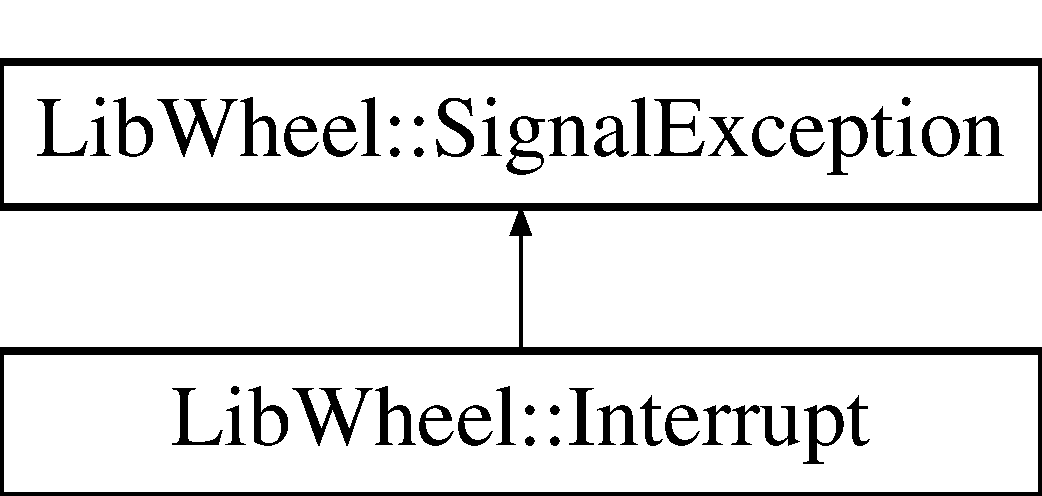
\includegraphics[height=2.000000cm]{classLibWheel_1_1SignalException}
\end{center}
\end{figure}
\subsection*{\-Public \-Member \-Functions}
\begin{DoxyCompactItemize}
\item 
virtual \hyperlink{classLibWheel_1_1SignalException_ade84b65584b146e9402ab0692921d0b4}{$\sim$\-Signal\-Exception} ()  throw ()
\begin{DoxyCompactList}\small\item\em \-Destructor for \hyperlink{classLibWheel_1_1SignalException}{\-Signal\-Exception}. \end{DoxyCompactList}\item 
const siginfo\-\_\-t $\ast$ \hyperlink{classLibWheel_1_1SignalException_a470409aa1db7608623c601c9bda573f4}{get\-Info} () const   throw ()
\begin{DoxyCompactList}\small\item\em \-Retrieve the details of a the signal represented by this \hyperlink{classLibWheel_1_1SignalException}{\-Signal\-Exception}. \end{DoxyCompactList}\item 
virtual const char $\ast$ \hyperlink{classLibWheel_1_1SignalException_a65ea3c23ec24f6448fb02624f9b039c2}{what} () const   throw ()
\begin{DoxyCompactList}\small\item\em \-Retrieve the description of the this exception. \end{DoxyCompactList}\item 
int \hyperlink{classLibWheel_1_1SignalException_a966b7c3d4054dd0a6c5121ae6d17d8cb}{get\-Signal\-Number} () const   throw ()
\begin{DoxyCompactList}\small\item\em \-Retrieve the signal number represented by this \hyperlink{classLibWheel_1_1SignalException}{\-Signal\-Exception}. \end{DoxyCompactList}\end{DoxyCompactItemize}
\subsection*{\-Protected \-Member \-Functions}
\begin{DoxyCompactItemize}
\item 
\hyperlink{classLibWheel_1_1SignalException_a6dec8b8da98fa48504123e7224d50a97}{\-Signal\-Exception} (int signum)  throw ()
\begin{DoxyCompactList}\small\item\em \-Constructor for \hyperlink{classLibWheel_1_1SignalException}{\-Signal\-Exception}. \end{DoxyCompactList}\item 
\hyperlink{classLibWheel_1_1SignalException_ae6be47f1a5842eb753c4f3e6b2e08e38}{\-Signal\-Exception} (int signum, const char $\ast$desc)  throw ()
\begin{DoxyCompactList}\small\item\em \-Constructor for \hyperlink{classLibWheel_1_1SignalException}{\-Signal\-Exception}. \end{DoxyCompactList}\item 
\hyperlink{classLibWheel_1_1SignalException_ad0132d99a0decc74c6c59c782340713f}{\-Signal\-Exception} (int signum, const char $\ast$desc, const siginfo\-\_\-t $\ast$info)  throw ()
\begin{DoxyCompactList}\small\item\em \-Constructor for \hyperlink{classLibWheel_1_1SignalException}{\-Signal\-Exception}. \end{DoxyCompactList}\end{DoxyCompactItemize}
\subsection*{\-Private \-Attributes}
\begin{DoxyCompactItemize}
\item 
const std\-::string \hyperlink{classLibWheel_1_1SignalException_a859cd244b034ef6514d695d233463049}{description}
\begin{DoxyCompactList}\small\item\em \-Description of the event triggering the exception. \end{DoxyCompactList}\item 
const siginfo\-\_\-t $\ast$ \hyperlink{classLibWheel_1_1SignalException_a687eb8c7e9e577738968313c1be0cd5b}{siginfo}
\begin{DoxyCompactList}\small\item\em \-Signal details, if available. \end{DoxyCompactList}\item 
const int \hyperlink{classLibWheel_1_1SignalException_a252b673e5b01bd416b2edbe38eeaac28}{number}
\begin{DoxyCompactList}\small\item\em \-Signal number. \end{DoxyCompactList}\end{DoxyCompactItemize}


\subsection{\-Detailed \-Description}
\-Base class for exceptions thrown by signal handlers. 

\subsection{\-Constructor \& \-Destructor \-Documentation}
\hypertarget{classLibWheel_1_1SignalException_a6dec8b8da98fa48504123e7224d50a97}{
\index{\-Lib\-Wheel\-::\-Signal\-Exception@{\-Lib\-Wheel\-::\-Signal\-Exception}!\-Signal\-Exception@{\-Signal\-Exception}}
\index{\-Signal\-Exception@{\-Signal\-Exception}!LibWheel::SignalException@{\-Lib\-Wheel\-::\-Signal\-Exception}}
\subsubsection[{\-Signal\-Exception}]{\setlength{\rightskip}{0pt plus 5cm}\-Lib\-Wheel\-::\-Signal\-Exception\-::\-Signal\-Exception (
\begin{DoxyParamCaption}
\item[{int}]{signum}
\end{DoxyParamCaption}
)  throw ()\hspace{0.3cm}{\ttfamily  \mbox{[}protected\mbox{]}}}}
\label{classLibWheel_1_1SignalException_a6dec8b8da98fa48504123e7224d50a97}


\-Constructor for \hyperlink{classLibWheel_1_1SignalException}{\-Signal\-Exception}. 


\begin{DoxyParams}{\-Parameters}
{\em signum} & \-The signal number represented by this \hyperlink{classLibWheel_1_1SignalException}{\-Signal\-Exception}. \\
\hline
\end{DoxyParams}


\-Definition at line 60 of file \-Signals.\-cpp.

\hypertarget{classLibWheel_1_1SignalException_ae6be47f1a5842eb753c4f3e6b2e08e38}{
\index{\-Lib\-Wheel\-::\-Signal\-Exception@{\-Lib\-Wheel\-::\-Signal\-Exception}!\-Signal\-Exception@{\-Signal\-Exception}}
\index{\-Signal\-Exception@{\-Signal\-Exception}!LibWheel::SignalException@{\-Lib\-Wheel\-::\-Signal\-Exception}}
\subsubsection[{\-Signal\-Exception}]{\setlength{\rightskip}{0pt plus 5cm}\-Lib\-Wheel\-::\-Signal\-Exception\-::\-Signal\-Exception (
\begin{DoxyParamCaption}
\item[{int}]{signum, }
\item[{const char $\ast$}]{desc}
\end{DoxyParamCaption}
)  throw ()\hspace{0.3cm}{\ttfamily  \mbox{[}protected\mbox{]}}}}
\label{classLibWheel_1_1SignalException_ae6be47f1a5842eb753c4f3e6b2e08e38}


\-Constructor for \hyperlink{classLibWheel_1_1SignalException}{\-Signal\-Exception}. 


\begin{DoxyParams}{\-Parameters}
{\em signum} & \-The signal number represented by this \hyperlink{classLibWheel_1_1SignalException}{\-Signal\-Exception}. \\
\hline
{\em desc} & \-A description of the exception. \\
\hline
\end{DoxyParams}


\-Definition at line 51 of file \-Signals.\-cpp.

\hypertarget{classLibWheel_1_1SignalException_ad0132d99a0decc74c6c59c782340713f}{
\index{\-Lib\-Wheel\-::\-Signal\-Exception@{\-Lib\-Wheel\-::\-Signal\-Exception}!\-Signal\-Exception@{\-Signal\-Exception}}
\index{\-Signal\-Exception@{\-Signal\-Exception}!LibWheel::SignalException@{\-Lib\-Wheel\-::\-Signal\-Exception}}
\subsubsection[{\-Signal\-Exception}]{\setlength{\rightskip}{0pt plus 5cm}\-Lib\-Wheel\-::\-Signal\-Exception\-::\-Signal\-Exception (
\begin{DoxyParamCaption}
\item[{int}]{signum, }
\item[{const char $\ast$}]{desc, }
\item[{const siginfo\-\_\-t $\ast$}]{info}
\end{DoxyParamCaption}
)  throw ()\hspace{0.3cm}{\ttfamily  \mbox{[}protected\mbox{]}}}}
\label{classLibWheel_1_1SignalException_ad0132d99a0decc74c6c59c782340713f}


\-Constructor for \hyperlink{classLibWheel_1_1SignalException}{\-Signal\-Exception}. 


\begin{DoxyParams}{\-Parameters}
{\em signum} & \-The signal number represented by this \hyperlink{classLibWheel_1_1SignalException}{\-Signal\-Exception}. \\
\hline
{\em desc} & \-A description of the exception. \\
\hline
{\em info} & \-Signal details. \\
\hline
\end{DoxyParams}


\-Definition at line 41 of file \-Signals.\-cpp.

\hypertarget{classLibWheel_1_1SignalException_ade84b65584b146e9402ab0692921d0b4}{
\index{\-Lib\-Wheel\-::\-Signal\-Exception@{\-Lib\-Wheel\-::\-Signal\-Exception}!$\sim$\-Signal\-Exception@{$\sim$\-Signal\-Exception}}
\index{$\sim$\-Signal\-Exception@{$\sim$\-Signal\-Exception}!LibWheel::SignalException@{\-Lib\-Wheel\-::\-Signal\-Exception}}
\subsubsection[{$\sim$\-Signal\-Exception}]{\setlength{\rightskip}{0pt plus 5cm}\-Lib\-Wheel\-::\-Signal\-Exception\-::$\sim$\-Signal\-Exception (
\begin{DoxyParamCaption}
{}
\end{DoxyParamCaption}
)  throw ()\hspace{0.3cm}{\ttfamily  \mbox{[}virtual\mbox{]}}}}
\label{classLibWheel_1_1SignalException_ade84b65584b146e9402ab0692921d0b4}


\-Destructor for \hyperlink{classLibWheel_1_1SignalException}{\-Signal\-Exception}. 



\-Definition at line 68 of file \-Signals.\-cpp.



\subsection{\-Member \-Function \-Documentation}
\hypertarget{classLibWheel_1_1SignalException_a470409aa1db7608623c601c9bda573f4}{
\index{\-Lib\-Wheel\-::\-Signal\-Exception@{\-Lib\-Wheel\-::\-Signal\-Exception}!get\-Info@{get\-Info}}
\index{get\-Info@{get\-Info}!LibWheel::SignalException@{\-Lib\-Wheel\-::\-Signal\-Exception}}
\subsubsection[{get\-Info}]{\setlength{\rightskip}{0pt plus 5cm}const siginfo\-\_\-t $\ast$ \-Lib\-Wheel\-::\-Signal\-Exception\-::get\-Info (
\begin{DoxyParamCaption}
{}
\end{DoxyParamCaption}
) const  throw ()}}
\label{classLibWheel_1_1SignalException_a470409aa1db7608623c601c9bda573f4}


\-Retrieve the details of a the signal represented by this \hyperlink{classLibWheel_1_1SignalException}{\-Signal\-Exception}. 

\-See the man page for sigaction() for details on the contents of a {\ttfamily siginfo\-\_\-t}. \begin{DoxyReturn}{\-Returns}
\-A pointer to the details, or \-N\-U\-L\-L if they're not available. 
\end{DoxyReturn}


\-Definition at line 79 of file \-Signals.\-cpp.



\-References siginfo.

\hypertarget{classLibWheel_1_1SignalException_a966b7c3d4054dd0a6c5121ae6d17d8cb}{
\index{\-Lib\-Wheel\-::\-Signal\-Exception@{\-Lib\-Wheel\-::\-Signal\-Exception}!get\-Signal\-Number@{get\-Signal\-Number}}
\index{get\-Signal\-Number@{get\-Signal\-Number}!LibWheel::SignalException@{\-Lib\-Wheel\-::\-Signal\-Exception}}
\subsubsection[{get\-Signal\-Number}]{\setlength{\rightskip}{0pt plus 5cm}int \-Lib\-Wheel\-::\-Signal\-Exception\-::get\-Signal\-Number (
\begin{DoxyParamCaption}
{}
\end{DoxyParamCaption}
) const  throw ()}}
\label{classLibWheel_1_1SignalException_a966b7c3d4054dd0a6c5121ae6d17d8cb}


\-Retrieve the signal number represented by this \hyperlink{classLibWheel_1_1SignalException}{\-Signal\-Exception}. 

\begin{DoxyReturn}{\-Returns}
\-The signal number. 
\end{DoxyReturn}


\-Definition at line 101 of file \-Signals.\-cpp.



\-References number.

\hypertarget{classLibWheel_1_1SignalException_a65ea3c23ec24f6448fb02624f9b039c2}{
\index{\-Lib\-Wheel\-::\-Signal\-Exception@{\-Lib\-Wheel\-::\-Signal\-Exception}!what@{what}}
\index{what@{what}!LibWheel::SignalException@{\-Lib\-Wheel\-::\-Signal\-Exception}}
\subsubsection[{what}]{\setlength{\rightskip}{0pt plus 5cm}const char $\ast$ \-Lib\-Wheel\-::\-Signal\-Exception\-::what (
\begin{DoxyParamCaption}
{}
\end{DoxyParamCaption}
) const  throw ()\hspace{0.3cm}{\ttfamily  \mbox{[}virtual\mbox{]}}}}
\label{classLibWheel_1_1SignalException_a65ea3c23ec24f6448fb02624f9b039c2}


\-Retrieve the description of the this exception. 

\begin{DoxyReturn}{\-Returns}
\-A pointer to the description, which may be an empty string. 
\end{DoxyReturn}


\-Definition at line 90 of file \-Signals.\-cpp.



\-References description.



\subsection{\-Member \-Data \-Documentation}
\hypertarget{classLibWheel_1_1SignalException_a859cd244b034ef6514d695d233463049}{
\index{\-Lib\-Wheel\-::\-Signal\-Exception@{\-Lib\-Wheel\-::\-Signal\-Exception}!description@{description}}
\index{description@{description}!LibWheel::SignalException@{\-Lib\-Wheel\-::\-Signal\-Exception}}
\subsubsection[{description}]{\setlength{\rightskip}{0pt plus 5cm}const std\-::string {\bf \-Lib\-Wheel\-::\-Signal\-Exception\-::description}\hspace{0.3cm}{\ttfamily  \mbox{[}private\mbox{]}}}}
\label{classLibWheel_1_1SignalException_a859cd244b034ef6514d695d233463049}


\-Description of the event triggering the exception. 



\-Definition at line 40 of file \-Signals.\-hpp.



\-Referenced by what().

\hypertarget{classLibWheel_1_1SignalException_a252b673e5b01bd416b2edbe38eeaac28}{
\index{\-Lib\-Wheel\-::\-Signal\-Exception@{\-Lib\-Wheel\-::\-Signal\-Exception}!number@{number}}
\index{number@{number}!LibWheel::SignalException@{\-Lib\-Wheel\-::\-Signal\-Exception}}
\subsubsection[{number}]{\setlength{\rightskip}{0pt plus 5cm}const int {\bf \-Lib\-Wheel\-::\-Signal\-Exception\-::number}\hspace{0.3cm}{\ttfamily  \mbox{[}private\mbox{]}}}}
\label{classLibWheel_1_1SignalException_a252b673e5b01bd416b2edbe38eeaac28}


\-Signal number. 



\-Definition at line 42 of file \-Signals.\-hpp.



\-Referenced by get\-Signal\-Number().

\hypertarget{classLibWheel_1_1SignalException_a687eb8c7e9e577738968313c1be0cd5b}{
\index{\-Lib\-Wheel\-::\-Signal\-Exception@{\-Lib\-Wheel\-::\-Signal\-Exception}!siginfo@{siginfo}}
\index{siginfo@{siginfo}!LibWheel::SignalException@{\-Lib\-Wheel\-::\-Signal\-Exception}}
\subsubsection[{siginfo}]{\setlength{\rightskip}{0pt plus 5cm}const siginfo\-\_\-t$\ast$ {\bf \-Lib\-Wheel\-::\-Signal\-Exception\-::siginfo}\hspace{0.3cm}{\ttfamily  \mbox{[}private\mbox{]}}}}
\label{classLibWheel_1_1SignalException_a687eb8c7e9e577738968313c1be0cd5b}


\-Signal details, if available. 



\-Definition at line 41 of file \-Signals.\-hpp.



\-Referenced by get\-Info().



\-The documentation for this class was generated from the following files\-:\begin{DoxyCompactItemize}
\item 
\hyperlink{Signals_8hpp}{\-Signals.\-hpp}\item 
\hyperlink{Signals_8cpp}{\-Signals.\-cpp}\end{DoxyCompactItemize}

\hypertarget{classLibWheel_1_1SignalQueue}{
\section{\-Lib\-Wheel\-:\-:\-Signal\-Queue \-Class \-Reference}
\label{classLibWheel_1_1SignalQueue}\index{\-Lib\-Wheel\-::\-Signal\-Queue@{\-Lib\-Wheel\-::\-Signal\-Queue}}
}


\-A system for synchronously handling asynchronous signals in a uni-\/threaded process.  




{\ttfamily \#include $<$\-Signals.\-hpp$>$}

\subsection*{\-Classes}
\begin{DoxyCompactItemize}
\item 
struct \hyperlink{structLibWheel_1_1SignalQueue_1_1Pipe}{\-Pipe}
\begin{DoxyCompactList}\small\item\em \-Convienience wrapper for a non-\/blocking \-Unix pipe. \end{DoxyCompactList}\end{DoxyCompactItemize}
\subsection*{\-Public \-Types}
\begin{DoxyCompactItemize}
\item 
enum \hyperlink{classLibWheel_1_1SignalQueue_a5a366bd8de3564c5e3001233464d20e3}{\-Action} \{ \hyperlink{classLibWheel_1_1SignalQueue_a5a366bd8de3564c5e3001233464d20e3a999854ec907bcd96c6948c5fab16337a}{\-D\-E\-F\-A\-U\-L\-T}, 
\hyperlink{classLibWheel_1_1SignalQueue_a5a366bd8de3564c5e3001233464d20e3a57f9c96915e2cbabc7c7ea653a43bc83}{\-I\-G\-N\-O\-R\-E}, 
\hyperlink{classLibWheel_1_1SignalQueue_a5a366bd8de3564c5e3001233464d20e3a4ee98693cfe0961ea7dcfac5f2053174}{\-H\-A\-N\-D\-L\-E}
 \}
\begin{DoxyCompactList}\small\item\em \-Possible ways to handle a signal. \end{DoxyCompactList}\end{DoxyCompactItemize}
\subsection*{\-Static \-Public \-Member \-Functions}
\begin{DoxyCompactItemize}
\item 
static void \hyperlink{classLibWheel_1_1SignalQueue_ac0145e9276c339fccebe3c0b70cec914}{set\-Handler} (int sig, \hyperlink{classLibWheel_1_1SignalQueue_a5a366bd8de3564c5e3001233464d20e3}{\-Action} act)  throw (std\-::domain\-\_\-error, std\-::invalid\-\_\-argument)
\begin{DoxyCompactList}\small\item\em \-Set the action to perform when a signal is received. \end{DoxyCompactList}\item 
static void \hyperlink{classLibWheel_1_1SignalQueue_ada6b998cee9ced93ac7e046199187fa6}{add\-Handler} (int sig, boost\-::function$<$ void()$>$ act)  throw (std\-::invalid\-\_\-argument)
\begin{DoxyCompactList}\small\item\em \-Add a handler function for a signal. \end{DoxyCompactList}\item 
{\footnotesize template$<$typename T $>$ }\\static void \hyperlink{classLibWheel_1_1SignalQueue_a16b57819e9a601533b9bff97ec08b5e5}{delete\-Handler} (int sig, const \-T \&act)  throw (std\-::invalid\-\_\-argument)
\begin{DoxyCompactList}\small\item\em \-Unregister a handler for a signal. \end{DoxyCompactList}\item 
static void \hyperlink{classLibWheel_1_1SignalQueue_afc29a5340fe52fd173e808f65f0ec3a7}{delete\-Handlers} (int sig)  throw (std\-::invalid\-\_\-argument)
\begin{DoxyCompactList}\small\item\em \-Remove all handlers for a signal. \end{DoxyCompactList}\item 
static void \hyperlink{classLibWheel_1_1SignalQueue_a991ba21066232f0db7be5f21e39edc41}{handle\-Next} ()
\begin{DoxyCompactList}\small\item\em \-Call all handlers for the next signal in the signal pipe. \end{DoxyCompactList}\item 
static void \hyperlink{classLibWheel_1_1SignalQueue_ad308bc4818a9d864bc0eb7b4dd1490ae}{handle\-All} ()
\begin{DoxyCompactList}\small\item\em \-Call all handlers for all signals in the signal pipe. \end{DoxyCompactList}\item 
static bool \hyperlink{classLibWheel_1_1SignalQueue_afd382f0a75d89bb0b6a22d9899c4435e}{pending} ()  throw (std\-::runtime\-\_\-error)
\begin{DoxyCompactList}\small\item\em \-Check if any signals are pending in the signal queue. \end{DoxyCompactList}\item 
static int \hyperlink{classLibWheel_1_1SignalQueue_a36582b3985b30c6620ed3476b97e8538}{get\-Read\-F\-D} ()
\begin{DoxyCompactList}\small\item\em \-Retrieve the read file descriptor of the signal pipe. \end{DoxyCompactList}\item 
static int \hyperlink{classLibWheel_1_1SignalQueue_a8ba3b23aab26d744bcc2bffcc6598921}{select} (int n, fd\-\_\-set $\ast$readfds, fd\-\_\-set $\ast$writefds, fd\-\_\-set $\ast$exceptfds, struct timeval $\ast$timeout)
\begin{DoxyCompactList}\small\item\em \-Wait for an event to occur on a file descriptor. \end{DoxyCompactList}\end{DoxyCompactItemize}
\subsection*{\-Private \-Types}
\begin{DoxyCompactItemize}
\item 
typedef std\-::list\*
$<$ boost\-::function$<$ void()$>$ $>$ \hyperlink{classLibWheel_1_1SignalQueue_a4bfc25c5e467e668c89ee0b0ceaa7591}{\-Handler\-List}
\begin{DoxyCompactList}\small\item\em \-The type of a set of handlers for a particular signal. \end{DoxyCompactList}\end{DoxyCompactItemize}
\subsection*{\-Private \-Member \-Functions}
\begin{DoxyCompactItemize}
\item 
friend \hyperlink{classLibWheel_1_1SignalQueue_ab219a09c14ff06e916c70dbdabdbf28a}{void\-::\-Signal\-Queue\-\_\-signal\-Handler} (int, siginfo\-\_\-t $\ast$, void $\ast$)
\begin{DoxyCompactList}\small\item\em \-This needs to call \hyperlink{classLibWheel_1_1SignalQueue_a522c461293731cec36208aa3bafe39c7}{get\-Signal\-Pipe()}. \end{DoxyCompactList}\end{DoxyCompactItemize}
\subsection*{\-Static \-Private \-Member \-Functions}
\begin{DoxyCompactItemize}
\item 
static const \hyperlink{structLibWheel_1_1SignalQueue_1_1Pipe}{\-Pipe} \& \hyperlink{classLibWheel_1_1SignalQueue_a522c461293731cec36208aa3bafe39c7}{get\-Signal\-Pipe} ()
\begin{DoxyCompactList}\small\item\em \-Retrieve the signal pipe used by \hyperlink{classLibWheel_1_1SignalQueue}{\-Signal\-Queue}. \end{DoxyCompactList}\item 
static \hyperlink{classLibWheel_1_1SignalQueue_a4bfc25c5e467e668c89ee0b0ceaa7591}{\-Handler\-List} $\ast$ \hyperlink{classLibWheel_1_1SignalQueue_a0e04644ce369cc519197043735986f9c}{get\-Signal\-Table} ()
\begin{DoxyCompactList}\small\item\em \-Retrieve the table of signal handlers. \end{DoxyCompactList}\end{DoxyCompactItemize}


\subsection{\-Detailed \-Description}
\-A system for synchronously handling asynchronous signals in a uni-\/threaded process. 

\-Users can request that certain signals be handled, and can register any number of arbitrary functions to handle them. \-When a signal arrives, all that is done is that its number is written to a pipe. \-The user can then poll for pending signals from the pipe using \hyperlink{classLibWheel_1_1SignalQueue_afd382f0a75d89bb0b6a22d9899c4435e}{\-Signal\-Queue\-::pending()} or by calling {\ttfamily poll()} or {\ttfamily select}() on \hyperlink{classLibWheel_1_1SignalQueue_a36582b3985b30c6620ed3476b97e8538}{\-Signal\-Queue\-::get\-Read\-F\-D()}, and can execute all handlers for pending signals using \hyperlink{classLibWheel_1_1SignalQueue_a991ba21066232f0db7be5f21e39edc41}{\-Signal\-Queue\-::handle\-Next()} and \hyperlink{classLibWheel_1_1SignalQueue_ad308bc4818a9d864bc0eb7b4dd1490ae}{\-Signal\-Queue\-::handle\-All()}. \-Handlers are executed in the order that they were registered. \hyperlink{classLibWheel_1_1SignalQueue_a8ba3b23aab26d744bcc2bffcc6598921}{\-Signal\-Queue\-::select()} is provided as an version of {\ttfamily select}() that waits for file descriptors to change status, while handling any signals that arrive in the meantime.

\-Signal handlers can be either functions or functors that take no parameters and return {\ttfamily void}. \-Since they are called synchronously from normal program flow, they can safely perform any action, including throw exceptions. (\hyperlink{classLibWheel_1_1SignalException}{\-Signal\-Exception} is provided for this purpose.)

\-Since \hyperlink{classLibWheel_1_1SignalQueue}{\-Signal\-Queue} only has static methods, it could simply be a namespace (rather than a class). \-However, \-I couldn't get a non-\/template version of \hyperlink{classLibWheel_1_1SignalQueue_a16b57819e9a601533b9bff97ec08b5e5}{delete\-Handler()} to work properly, so its definition needs to be inline, and it needs to call \hyperlink{classLibWheel_1_1SignalQueue_a0e04644ce369cc519197043735986f9c}{get\-Signal\-Table()}, which should be private. \-If this was a namespace, \hyperlink{classLibWheel_1_1SignalQueue_a0e04644ce369cc519197043735986f9c}{get\-Signal\-Table()} and all the other private stuff could be static to \hyperlink{Signals_8cpp}{\-Signals.\-cpp}. 

\subsection{\-Member \-Typedef \-Documentation}
\hypertarget{classLibWheel_1_1SignalQueue_a4bfc25c5e467e668c89ee0b0ceaa7591}{
\index{\-Lib\-Wheel\-::\-Signal\-Queue@{\-Lib\-Wheel\-::\-Signal\-Queue}!\-Handler\-List@{\-Handler\-List}}
\index{\-Handler\-List@{\-Handler\-List}!LibWheel::SignalQueue@{\-Lib\-Wheel\-::\-Signal\-Queue}}
\subsubsection[{\-Handler\-List}]{\setlength{\rightskip}{0pt plus 5cm}typedef std\-::list$<$boost\-::function$<$void()$>$ $>$ {\bf \-Lib\-Wheel\-::\-Signal\-Queue\-::\-Handler\-List}\hspace{0.3cm}{\ttfamily  \mbox{[}private\mbox{]}}}}
\label{classLibWheel_1_1SignalQueue_a4bfc25c5e467e668c89ee0b0ceaa7591}


\-The type of a set of handlers for a particular signal. 



\-Definition at line 120 of file \-Signals.\-hpp.



\subsection{\-Member \-Enumeration \-Documentation}
\hypertarget{classLibWheel_1_1SignalQueue_a5a366bd8de3564c5e3001233464d20e3}{
\index{\-Lib\-Wheel\-::\-Signal\-Queue@{\-Lib\-Wheel\-::\-Signal\-Queue}!\-Action@{\-Action}}
\index{\-Action@{\-Action}!LibWheel::SignalQueue@{\-Lib\-Wheel\-::\-Signal\-Queue}}
\subsubsection[{\-Action}]{\setlength{\rightskip}{0pt plus 5cm}enum {\bf \-Lib\-Wheel\-::\-Signal\-Queue\-::\-Action}}}
\label{classLibWheel_1_1SignalQueue_a5a366bd8de3564c5e3001233464d20e3}


\-Possible ways to handle a signal. 

\begin{Desc}
\item[\-Enumerator\-: ]\par
\begin{description}
\index{\-D\-E\-F\-A\-U\-L\-T@{\-D\-E\-F\-A\-U\-L\-T}!\-Lib\-Wheel\-::\-Signal\-Queue@{\-Lib\-Wheel\-::\-Signal\-Queue}}\index{\-Lib\-Wheel\-::\-Signal\-Queue@{\-Lib\-Wheel\-::\-Signal\-Queue}!\-D\-E\-F\-A\-U\-L\-T@{\-D\-E\-F\-A\-U\-L\-T}}\item[{\em 
\hypertarget{classLibWheel_1_1SignalQueue_a5a366bd8de3564c5e3001233464d20e3a999854ec907bcd96c6948c5fab16337a}{
\-D\-E\-F\-A\-U\-L\-T}
\label{classLibWheel_1_1SignalQueue_a5a366bd8de3564c5e3001233464d20e3a999854ec907bcd96c6948c5fab16337a}
}]\-Take the operating systems's default action for the signal. \index{\-I\-G\-N\-O\-R\-E@{\-I\-G\-N\-O\-R\-E}!\-Lib\-Wheel\-::\-Signal\-Queue@{\-Lib\-Wheel\-::\-Signal\-Queue}}\index{\-Lib\-Wheel\-::\-Signal\-Queue@{\-Lib\-Wheel\-::\-Signal\-Queue}!\-I\-G\-N\-O\-R\-E@{\-I\-G\-N\-O\-R\-E}}\item[{\em 
\hypertarget{classLibWheel_1_1SignalQueue_a5a366bd8de3564c5e3001233464d20e3a57f9c96915e2cbabc7c7ea653a43bc83}{
\-I\-G\-N\-O\-R\-E}
\label{classLibWheel_1_1SignalQueue_a5a366bd8de3564c5e3001233464d20e3a57f9c96915e2cbabc7c7ea653a43bc83}
}]\-Ignore the signal. \index{\-H\-A\-N\-D\-L\-E@{\-H\-A\-N\-D\-L\-E}!\-Lib\-Wheel\-::\-Signal\-Queue@{\-Lib\-Wheel\-::\-Signal\-Queue}}\index{\-Lib\-Wheel\-::\-Signal\-Queue@{\-Lib\-Wheel\-::\-Signal\-Queue}!\-H\-A\-N\-D\-L\-E@{\-H\-A\-N\-D\-L\-E}}\item[{\em 
\hypertarget{classLibWheel_1_1SignalQueue_a5a366bd8de3564c5e3001233464d20e3a4ee98693cfe0961ea7dcfac5f2053174}{
\-H\-A\-N\-D\-L\-E}
\label{classLibWheel_1_1SignalQueue_a5a366bd8de3564c5e3001233464d20e3a4ee98693cfe0961ea7dcfac5f2053174}
}]\-Call all registered signal handlers when a signal is received. \end{description}
\end{Desc}



\-Definition at line 129 of file \-Signals.\-hpp.



\subsection{\-Member \-Function \-Documentation}
\hypertarget{classLibWheel_1_1SignalQueue_ada6b998cee9ced93ac7e046199187fa6}{
\index{\-Lib\-Wheel\-::\-Signal\-Queue@{\-Lib\-Wheel\-::\-Signal\-Queue}!add\-Handler@{add\-Handler}}
\index{add\-Handler@{add\-Handler}!LibWheel::SignalQueue@{\-Lib\-Wheel\-::\-Signal\-Queue}}
\subsubsection[{add\-Handler}]{\setlength{\rightskip}{0pt plus 5cm}void \-Lib\-Wheel\-::\-Signal\-Queue\-::add\-Handler (
\begin{DoxyParamCaption}
\item[{int}]{sig, }
\item[{boost\-::function$<$ void()$>$}]{act}
\end{DoxyParamCaption}
)  throw (std\-::invalid\-\_\-argument)\hspace{0.3cm}{\ttfamily  \mbox{[}static\mbox{]}}}}
\label{classLibWheel_1_1SignalQueue_ada6b998cee9ced93ac7e046199187fa6}


\-Add a handler function for a signal. 


\begin{DoxyParams}{\-Parameters}
{\em sig} & \-The signal for which the handler is to be added. \\
\hline
{\em act} & \-The handler to add. \\
\hline
\end{DoxyParams}

\begin{DoxyExceptions}{\-Exceptions}
{\em std\-::invalid\-\_\-argument} & \-If {\itshape sig\/} is invalid. \\
\hline
\end{DoxyExceptions}


\-Definition at line 234 of file \-Signals.\-cpp.



\-References get\-Signal\-Table().



\-Referenced by \-N\-E\-R\-D\-::\-Connection\-Server\-::\-Connection\-Server(), main(), \-Lib\-Wheel\-::\-Timer\-::\-Timer(), and \-Lib\-Wheel\-::\-Wait\-List\-::\-Wait\-List().

\hypertarget{classLibWheel_1_1SignalQueue_a16b57819e9a601533b9bff97ec08b5e5}{
\index{\-Lib\-Wheel\-::\-Signal\-Queue@{\-Lib\-Wheel\-::\-Signal\-Queue}!delete\-Handler@{delete\-Handler}}
\index{delete\-Handler@{delete\-Handler}!LibWheel::SignalQueue@{\-Lib\-Wheel\-::\-Signal\-Queue}}
\subsubsection[{delete\-Handler}]{\setlength{\rightskip}{0pt plus 5cm}template$<$typename T $>$ void \-Lib\-Wheel\-::\-Signal\-Queue\-::delete\-Handler (
\begin{DoxyParamCaption}
\item[{int}]{sig, }
\item[{const \-T \&}]{act}
\end{DoxyParamCaption}
)  throw (std\-::invalid\-\_\-argument)\hspace{0.3cm}{\ttfamily  \mbox{[}static\mbox{]}}}}
\label{classLibWheel_1_1SignalQueue_a16b57819e9a601533b9bff97ec08b5e5}


\-Unregister a handler for a signal. 


\begin{DoxyParams}{\-Parameters}
{\em sig} & \-A signal number. \\
\hline
{\em act} & \-A reference to the signal handler to unregister for {\itshape sig\/}. \\
\hline
\end{DoxyParams}

\begin{DoxyExceptions}{\-Exceptions}
{\em std\-::invalid\-\_\-argument} & \-If {\itshape sig\/} is not a valid signal number. \\
\hline
\end{DoxyExceptions}


\-Definition at line 156 of file \-Signals.\-hpp.



\-Referenced by \-N\-E\-R\-D\-::\-Connection\-Server\-::$\sim$\-Connection\-Server(), \-Lib\-Wheel\-::\-Timer\-::$\sim$\-Timer(), and \-Lib\-Wheel\-::\-Wait\-List\-::$\sim$\-Wait\-List().

\hypertarget{classLibWheel_1_1SignalQueue_afc29a5340fe52fd173e808f65f0ec3a7}{
\index{\-Lib\-Wheel\-::\-Signal\-Queue@{\-Lib\-Wheel\-::\-Signal\-Queue}!delete\-Handlers@{delete\-Handlers}}
\index{delete\-Handlers@{delete\-Handlers}!LibWheel::SignalQueue@{\-Lib\-Wheel\-::\-Signal\-Queue}}
\subsubsection[{delete\-Handlers}]{\setlength{\rightskip}{0pt plus 5cm}void \-Lib\-Wheel\-::\-Signal\-Queue\-::delete\-Handlers (
\begin{DoxyParamCaption}
\item[{int}]{sig}
\end{DoxyParamCaption}
)  throw (std\-::invalid\-\_\-argument)\hspace{0.3cm}{\ttfamily  \mbox{[}static\mbox{]}}}}
\label{classLibWheel_1_1SignalQueue_afc29a5340fe52fd173e808f65f0ec3a7}


\-Remove all handlers for a signal. 


\begin{DoxyParams}{\-Parameters}
{\em sig} & \-The signal whose handlers to remove. \\
\hline
\end{DoxyParams}

\begin{DoxyExceptions}{\-Exceptions}
{\em std\-::invalid\-\_\-argument} & \-If {\itshape sig\/} is invalid. \\
\hline
\end{DoxyExceptions}


\-Definition at line 249 of file \-Signals.\-cpp.



\-References get\-Signal\-Table().

\hypertarget{classLibWheel_1_1SignalQueue_a36582b3985b30c6620ed3476b97e8538}{
\index{\-Lib\-Wheel\-::\-Signal\-Queue@{\-Lib\-Wheel\-::\-Signal\-Queue}!get\-Read\-F\-D@{get\-Read\-F\-D}}
\index{get\-Read\-F\-D@{get\-Read\-F\-D}!LibWheel::SignalQueue@{\-Lib\-Wheel\-::\-Signal\-Queue}}
\subsubsection[{get\-Read\-F\-D}]{\setlength{\rightskip}{0pt plus 5cm}int \-Lib\-Wheel\-::\-Signal\-Queue\-::get\-Read\-F\-D (
\begin{DoxyParamCaption}
{}
\end{DoxyParamCaption}
)\hspace{0.3cm}{\ttfamily  \mbox{[}static\mbox{]}}}}
\label{classLibWheel_1_1SignalQueue_a36582b3985b30c6620ed3476b97e8538}


\-Retrieve the read file descriptor of the signal pipe. 

\-It may be used to poll for pending signals using {\ttfamily poll()} or {\ttfamily select}(); reading from it will cause signals to be lost. \begin{DoxyReturn}{\-Returns}
\-The file descriptor of the signal pipe. 
\end{DoxyReturn}


\-Definition at line 334 of file \-Signals.\-cpp.



\-References get\-Signal\-Pipe(), and \-Lib\-Wheel\-::\-Signal\-Queue\-::\-Pipe\-::fds.



\-Referenced by \-N\-E\-R\-D\-::\-Connection\-Server\-::operator()(), handle\-Next(), pending(), and select().

\hypertarget{classLibWheel_1_1SignalQueue_a522c461293731cec36208aa3bafe39c7}{
\index{\-Lib\-Wheel\-::\-Signal\-Queue@{\-Lib\-Wheel\-::\-Signal\-Queue}!get\-Signal\-Pipe@{get\-Signal\-Pipe}}
\index{get\-Signal\-Pipe@{get\-Signal\-Pipe}!LibWheel::SignalQueue@{\-Lib\-Wheel\-::\-Signal\-Queue}}
\subsubsection[{get\-Signal\-Pipe}]{\setlength{\rightskip}{0pt plus 5cm}const {\bf \-Signal\-Queue\-::\-Pipe} \& \-Lib\-Wheel\-::\-Signal\-Queue\-::get\-Signal\-Pipe (
\begin{DoxyParamCaption}
{}
\end{DoxyParamCaption}
)\hspace{0.3cm}{\ttfamily  \mbox{[}static, private\mbox{]}}}}
\label{classLibWheel_1_1SignalQueue_a522c461293731cec36208aa3bafe39c7}


\-Retrieve the signal pipe used by \hyperlink{classLibWheel_1_1SignalQueue}{\-Signal\-Queue}. 

\begin{DoxyReturn}{\-Returns}
\-A reference to \-Signal\-Queue's signal pipe. 
\end{DoxyReturn}


\-Definition at line 165 of file \-Signals.\-cpp.



\-Referenced by set\-Handler(), get\-Read\-F\-D(), and \-Signal\-Queue\-\_\-signal\-Handler().

\hypertarget{classLibWheel_1_1SignalQueue_a0e04644ce369cc519197043735986f9c}{
\index{\-Lib\-Wheel\-::\-Signal\-Queue@{\-Lib\-Wheel\-::\-Signal\-Queue}!get\-Signal\-Table@{get\-Signal\-Table}}
\index{get\-Signal\-Table@{get\-Signal\-Table}!LibWheel::SignalQueue@{\-Lib\-Wheel\-::\-Signal\-Queue}}
\subsubsection[{get\-Signal\-Table}]{\setlength{\rightskip}{0pt plus 5cm}{\bf \-Signal\-Queue\-::\-Handler\-List} $\ast$ \-Lib\-Wheel\-::\-Signal\-Queue\-::get\-Signal\-Table (
\begin{DoxyParamCaption}
{}
\end{DoxyParamCaption}
)\hspace{0.3cm}{\ttfamily  \mbox{[}static, private\mbox{]}}}}
\label{classLibWheel_1_1SignalQueue_a0e04644ce369cc519197043735986f9c}


\-Retrieve the table of signal handlers. 

\begin{DoxyReturn}{\-Returns}
\-A pointer to the signal handler table (an array of \-\_\-\-N\-S\-I\-G elements). 
\end{DoxyReturn}


\-Definition at line 178 of file \-Signals.\-cpp.



\-Referenced by add\-Handler(), delete\-Handlers(), and handle\-Next().

\hypertarget{classLibWheel_1_1SignalQueue_ad308bc4818a9d864bc0eb7b4dd1490ae}{
\index{\-Lib\-Wheel\-::\-Signal\-Queue@{\-Lib\-Wheel\-::\-Signal\-Queue}!handle\-All@{handle\-All}}
\index{handle\-All@{handle\-All}!LibWheel::SignalQueue@{\-Lib\-Wheel\-::\-Signal\-Queue}}
\subsubsection[{handle\-All}]{\setlength{\rightskip}{0pt plus 5cm}void \-Lib\-Wheel\-::\-Signal\-Queue\-::handle\-All (
\begin{DoxyParamCaption}
{}
\end{DoxyParamCaption}
)\hspace{0.3cm}{\ttfamily  \mbox{[}static\mbox{]}}}}
\label{classLibWheel_1_1SignalQueue_ad308bc4818a9d864bc0eb7b4dd1490ae}


\-Call all handlers for all signals in the signal pipe. 


\begin{DoxyExceptions}{\-Exceptions}
{\em \-Anything} & that a registered signal handler throws. \\
\hline
\end{DoxyExceptions}


\-Definition at line 293 of file \-Signals.\-cpp.



\-References pending(), and handle\-Next().



\-Referenced by select().

\hypertarget{classLibWheel_1_1SignalQueue_a991ba21066232f0db7be5f21e39edc41}{
\index{\-Lib\-Wheel\-::\-Signal\-Queue@{\-Lib\-Wheel\-::\-Signal\-Queue}!handle\-Next@{handle\-Next}}
\index{handle\-Next@{handle\-Next}!LibWheel::SignalQueue@{\-Lib\-Wheel\-::\-Signal\-Queue}}
\subsubsection[{handle\-Next}]{\setlength{\rightskip}{0pt plus 5cm}void \-Lib\-Wheel\-::\-Signal\-Queue\-::handle\-Next (
\begin{DoxyParamCaption}
{}
\end{DoxyParamCaption}
)\hspace{0.3cm}{\ttfamily  \mbox{[}static\mbox{]}}}}
\label{classLibWheel_1_1SignalQueue_a991ba21066232f0db7be5f21e39edc41}


\-Call all handlers for the next signal in the signal pipe. 


\begin{DoxyExceptions}{\-Exceptions}
{\em \-Anything} & that a registered signal handler throws. \\
\hline
\end{DoxyExceptions}


\-Definition at line 263 of file \-Signals.\-cpp.



\-References get\-Read\-F\-D(), and get\-Signal\-Table().



\-Referenced by \-N\-E\-R\-D\-::\-Connection\-Server\-::operator()(), and handle\-All().

\hypertarget{classLibWheel_1_1SignalQueue_afd382f0a75d89bb0b6a22d9899c4435e}{
\index{\-Lib\-Wheel\-::\-Signal\-Queue@{\-Lib\-Wheel\-::\-Signal\-Queue}!pending@{pending}}
\index{pending@{pending}!LibWheel::SignalQueue@{\-Lib\-Wheel\-::\-Signal\-Queue}}
\subsubsection[{pending}]{\setlength{\rightskip}{0pt plus 5cm}bool \-Lib\-Wheel\-::\-Signal\-Queue\-::pending (
\begin{DoxyParamCaption}
{}
\end{DoxyParamCaption}
)  throw (std\-::runtime\-\_\-error)\hspace{0.3cm}{\ttfamily  \mbox{[}static\mbox{]}}}}
\label{classLibWheel_1_1SignalQueue_afd382f0a75d89bb0b6a22d9899c4435e}


\-Check if any signals are pending in the signal queue. 

\begin{DoxyReturn}{\-Returns}
{\bfseries true} if a signal is pending; {\bfseries false} otherwise. 
\end{DoxyReturn}

\begin{DoxyExceptions}{\-Exceptions}
{\em std\-::runtime\-\_\-error} & \-If there is an error checking the signal queue. \\
\hline
\end{DoxyExceptions}


\-Definition at line 306 of file \-Signals.\-cpp.



\-References get\-Read\-F\-D(), and select().



\-Referenced by handle\-All().

\hypertarget{classLibWheel_1_1SignalQueue_a8ba3b23aab26d744bcc2bffcc6598921}{
\index{\-Lib\-Wheel\-::\-Signal\-Queue@{\-Lib\-Wheel\-::\-Signal\-Queue}!select@{select}}
\index{select@{select}!LibWheel::SignalQueue@{\-Lib\-Wheel\-::\-Signal\-Queue}}
\subsubsection[{select}]{\setlength{\rightskip}{0pt plus 5cm}int \-Lib\-Wheel\-::\-Signal\-Queue\-::select (
\begin{DoxyParamCaption}
\item[{int}]{n, }
\item[{fd\-\_\-set $\ast$}]{readfds, }
\item[{fd\-\_\-set $\ast$}]{writefds, }
\item[{fd\-\_\-set $\ast$}]{exceptfds, }
\item[{struct timeval $\ast$}]{timeout}
\end{DoxyParamCaption}
)\hspace{0.3cm}{\ttfamily  \mbox{[}static\mbox{]}}}}
\label{classLibWheel_1_1SignalQueue_a8ba3b23aab26d744bcc2bffcc6598921}


\-Wait for an event to occur on a file descriptor. 

\-This works identically to select(), except that any signals that are delivered before an event occurs are handled. \-See the man page for select() for details. 
\begin{DoxyParams}{\-Parameters}
{\em n} & \-The highest-\/numbered file descriptor in {\itshape readfds\/}, {\itshape writefds\/} and {\itshape exceptfds\/}, plus 1. \\
\hline
{\em readfds} & \-A set of file descriptors to watch for avaiable data to read. \\
\hline
{\em writefds} & \-A set of file descriptors to watch for the possibility of writing data without blocking. \\
\hline
{\em exceptfds} & \-A set of file descriptors to watch for exceptional conditions. \\
\hline
{\em timeout} & \-An upper bound on the time to wait for events to occur. \-If it is zero, \hyperlink{classLibWheel_1_1SignalQueue_a8ba3b23aab26d744bcc2bffcc6598921}{select()} will return immediately. \-If it is null, \hyperlink{classLibWheel_1_1SignalQueue_a8ba3b23aab26d744bcc2bffcc6598921}{select()} will block indefinately. \\
\hline
\end{DoxyParams}


\-Definition at line 357 of file \-Signals.\-cpp.



\-References get\-Read\-F\-D(), and handle\-All().



\-Referenced by pending().

\hypertarget{classLibWheel_1_1SignalQueue_ac0145e9276c339fccebe3c0b70cec914}{
\index{\-Lib\-Wheel\-::\-Signal\-Queue@{\-Lib\-Wheel\-::\-Signal\-Queue}!set\-Handler@{set\-Handler}}
\index{set\-Handler@{set\-Handler}!LibWheel::SignalQueue@{\-Lib\-Wheel\-::\-Signal\-Queue}}
\subsubsection[{set\-Handler}]{\setlength{\rightskip}{0pt plus 5cm}void \-Lib\-Wheel\-::\-Signal\-Queue\-::set\-Handler (
\begin{DoxyParamCaption}
\item[{int}]{sig, }
\item[{{\bf \-Action}}]{act}
\end{DoxyParamCaption}
)  throw (std\-::domain\-\_\-error, std\-::invalid\-\_\-argument)\hspace{0.3cm}{\ttfamily  \mbox{[}static\mbox{]}}}}
\label{classLibWheel_1_1SignalQueue_ac0145e9276c339fccebe3c0b70cec914}


\-Set the action to perform when a signal is received. 


\begin{DoxyParams}{\-Parameters}
{\em sig} & \-The signal whose action to set. \\
\hline
{\em act} & \-The action to perform when {\itshape signal\/} is received. \\
\hline
\end{DoxyParams}

\begin{DoxyExceptions}{\-Exceptions}
{\em std\-::domain\-\_\-error} & \-If {\itshape act\/} is invalid. \\
\hline
{\em std\-::invalid\-\_\-argument} & \-If {\itshape sig\/} is invalid. \\
\hline
\end{DoxyExceptions}


\-Definition at line 193 of file \-Signals.\-cpp.



\-References \-D\-E\-F\-A\-U\-L\-T, \-I\-G\-N\-O\-R\-E, \-H\-A\-N\-D\-L\-E, \-Signal\-Queue\-\_\-signal\-Handler(), and get\-Signal\-Pipe().



\-Referenced by \-N\-E\-R\-D\-::\-Connection\-Server\-::\-Connection\-Server(), main(), \-Lib\-Wheel\-::\-Timer\-::\-Timer(), and \-Lib\-Wheel\-::\-Wait\-List\-::\-Wait\-List().

\hypertarget{classLibWheel_1_1SignalQueue_ab219a09c14ff06e916c70dbdabdbf28a}{
\index{\-Lib\-Wheel\-::\-Signal\-Queue@{\-Lib\-Wheel\-::\-Signal\-Queue}!void\-::\-Signal\-Queue\-\_\-signal\-Handler@{void\-::\-Signal\-Queue\-\_\-signal\-Handler}}
\index{void\-::\-Signal\-Queue\-\_\-signal\-Handler@{void\-::\-Signal\-Queue\-\_\-signal\-Handler}!LibWheel::SignalQueue@{\-Lib\-Wheel\-::\-Signal\-Queue}}
\subsubsection[{void\-::\-Signal\-Queue\-\_\-signal\-Handler}]{\setlength{\rightskip}{0pt plus 5cm}\-Lib\-Wheel\-::\-Signal\-Queue\-::void\-::\-Signal\-Queue\-\_\-signal\-Handler (
\begin{DoxyParamCaption}
\item[{int}]{, }
\item[{siginfo\-\_\-t $\ast$}]{, }
\item[{void $\ast$}]{}
\end{DoxyParamCaption}
)\hspace{0.3cm}{\ttfamily  \mbox{[}private\mbox{]}}}}
\label{classLibWheel_1_1SignalQueue_ab219a09c14ff06e916c70dbdabdbf28a}


\-This needs to call \hyperlink{classLibWheel_1_1SignalQueue_a522c461293731cec36208aa3bafe39c7}{get\-Signal\-Pipe()}. 



\-The documentation for this class was generated from the following files\-:\begin{DoxyCompactItemize}
\item 
\hyperlink{Signals_8hpp}{\-Signals.\-hpp}\item 
\hyperlink{Signals_8cpp}{\-Signals.\-cpp}\end{DoxyCompactItemize}

\hypertarget{classLibWheel_1_1SocketException}{
\section{\-Lib\-Wheel\-:\-:\-Socket\-Exception \-Class \-Reference}
\label{classLibWheel_1_1SocketException}\index{\-Lib\-Wheel\-::\-Socket\-Exception@{\-Lib\-Wheel\-::\-Socket\-Exception}}
}


\-Exception thrown when a socket error occurs.  




{\ttfamily \#include $<$util.\-hpp$>$}

\subsection*{\-Public \-Member \-Functions}
\begin{DoxyCompactItemize}
\item 
\hyperlink{classLibWheel_1_1SocketException_abcaca29d1baf285ab1a68177acd7313a}{\-Socket\-Exception} (const std\-::string \&s)
\begin{DoxyCompactList}\small\item\em \-Constructor for \hyperlink{classLibWheel_1_1SocketException}{\-Socket\-Exception}. \end{DoxyCompactList}\end{DoxyCompactItemize}


\subsection{\-Detailed \-Description}
\-Exception thrown when a socket error occurs. 

\subsection{\-Constructor \& \-Destructor \-Documentation}
\hypertarget{classLibWheel_1_1SocketException_abcaca29d1baf285ab1a68177acd7313a}{
\index{\-Lib\-Wheel\-::\-Socket\-Exception@{\-Lib\-Wheel\-::\-Socket\-Exception}!\-Socket\-Exception@{\-Socket\-Exception}}
\index{\-Socket\-Exception@{\-Socket\-Exception}!LibWheel::SocketException@{\-Lib\-Wheel\-::\-Socket\-Exception}}
\subsubsection[{\-Socket\-Exception}]{\setlength{\rightskip}{0pt plus 5cm}\-Lib\-Wheel\-::\-Socket\-Exception\-::\-Socket\-Exception (
\begin{DoxyParamCaption}
\item[{const std\-::string \&}]{s}
\end{DoxyParamCaption}
)}}
\label{classLibWheel_1_1SocketException_abcaca29d1baf285ab1a68177acd7313a}


\-Constructor for \hyperlink{classLibWheel_1_1SocketException}{\-Socket\-Exception}. 


\begin{DoxyParams}{\-Parameters}
{\em s} & \-A string describing the reason for throwing the exception. \\
\hline
\end{DoxyParams}


\-Definition at line 147 of file util.\-cpp.



\-The documentation for this class was generated from the following files\-:\begin{DoxyCompactItemize}
\item 
\hyperlink{util_8hpp}{util.\-hpp}\item 
\hyperlink{util_8cpp}{util.\-cpp}\end{DoxyCompactItemize}

\hypertarget{classNERD_1_1StatPrinter}{
\section{\-N\-E\-R\-D\-:\-:\-Stat\-Printer \-Class \-Reference}
\label{classNERD_1_1StatPrinter}\index{\-N\-E\-R\-D\-::\-Stat\-Printer@{\-N\-E\-R\-D\-::\-Stat\-Printer}}
}


\-Functor to print current server statistics.  


\subsection*{\-Public \-Member \-Functions}
\begin{DoxyCompactItemize}
\item 
\hyperlink{classNERD_1_1StatPrinter_a9e15d664037ee9b034a20e4a2c758e37}{\-Stat\-Printer} (const \hyperlink{classNERD_1_1ConnectionServer}{\-Connection\-Server} \&cs)
\begin{DoxyCompactList}\small\item\em \-Initialize a \hyperlink{classNERD_1_1StatPrinter}{\-Stat\-Printer}. \end{DoxyCompactList}\item 
void \hyperlink{classNERD_1_1StatPrinter_a276b7e4358a2cd8ec5a3972f86452d2c}{operator()} () const 
\begin{DoxyCompactList}\small\item\em \-Print the current statistics for a \hyperlink{classNERD_1_1ConnectionServer}{\-Connection\-Server}. \end{DoxyCompactList}\end{DoxyCompactItemize}
\subsection*{\-Private \-Attributes}
\begin{DoxyCompactItemize}
\item 
const \hyperlink{classNERD_1_1ConnectionServer}{\-Connection\-Server} \& \hyperlink{classNERD_1_1StatPrinter_a6040df27f017b5ce2ac0ed1d9f68d50b}{connection\-Server}
\begin{DoxyCompactList}\small\item\em \-A reference to a server object whose statistica are to be printed. \end{DoxyCompactList}\end{DoxyCompactItemize}


\subsection{\-Detailed \-Description}
\-Functor to print current server statistics. 

\subsection{\-Constructor \& \-Destructor \-Documentation}
\hypertarget{classNERD_1_1StatPrinter_a9e15d664037ee9b034a20e4a2c758e37}{
\index{\-N\-E\-R\-D\-::\-Stat\-Printer@{\-N\-E\-R\-D\-::\-Stat\-Printer}!\-Stat\-Printer@{\-Stat\-Printer}}
\index{\-Stat\-Printer@{\-Stat\-Printer}!NERD::StatPrinter@{\-N\-E\-R\-D\-::\-Stat\-Printer}}
\subsubsection[{\-Stat\-Printer}]{\setlength{\rightskip}{0pt plus 5cm}\-N\-E\-R\-D\-::\-Stat\-Printer\-::\-Stat\-Printer (
\begin{DoxyParamCaption}
\item[{const {\bf \-Connection\-Server} \&}]{cs}
\end{DoxyParamCaption}
)}}
\label{classNERD_1_1StatPrinter_a9e15d664037ee9b034a20e4a2c758e37}


\-Initialize a \hyperlink{classNERD_1_1StatPrinter}{\-Stat\-Printer}. 



\-Definition at line 1377 of file nerd.\-cpp.



\subsection{\-Member \-Function \-Documentation}
\hypertarget{classNERD_1_1StatPrinter_a276b7e4358a2cd8ec5a3972f86452d2c}{
\index{\-N\-E\-R\-D\-::\-Stat\-Printer@{\-N\-E\-R\-D\-::\-Stat\-Printer}!operator()@{operator()}}
\index{operator()@{operator()}!NERD::StatPrinter@{\-N\-E\-R\-D\-::\-Stat\-Printer}}
\subsubsection[{operator()}]{\setlength{\rightskip}{0pt plus 5cm}void \-N\-E\-R\-D\-::\-Stat\-Printer\-::operator() (
\begin{DoxyParamCaption}
{}
\end{DoxyParamCaption}
) const}}
\label{classNERD_1_1StatPrinter_a276b7e4358a2cd8ec5a3972f86452d2c}


\-Print the current statistics for a \hyperlink{classNERD_1_1ConnectionServer}{\-Connection\-Server}. 

\begin{DoxyParagraph}{\-Side \-Effects\-:}
\-Writes messages to \hyperlink{namespaceLibWheel_af4ca70f4f65b2948701218436516a679}{\-Lib\-Wheel\-::logmsg}. 
\end{DoxyParagraph}


\-Definition at line 1387 of file nerd.\-cpp.



\-References connection\-Server, and \-N\-E\-R\-D\-::\-Connection\-Server\-::print\-Stats().



\subsection{\-Member \-Data \-Documentation}
\hypertarget{classNERD_1_1StatPrinter_a6040df27f017b5ce2ac0ed1d9f68d50b}{
\index{\-N\-E\-R\-D\-::\-Stat\-Printer@{\-N\-E\-R\-D\-::\-Stat\-Printer}!connection\-Server@{connection\-Server}}
\index{connection\-Server@{connection\-Server}!NERD::StatPrinter@{\-N\-E\-R\-D\-::\-Stat\-Printer}}
\subsubsection[{connection\-Server}]{\setlength{\rightskip}{0pt plus 5cm}const {\bf \-Connection\-Server}\& {\bf \-N\-E\-R\-D\-::\-Stat\-Printer\-::connection\-Server}\hspace{0.3cm}{\ttfamily  \mbox{[}private\mbox{]}}}}
\label{classNERD_1_1StatPrinter_a6040df27f017b5ce2ac0ed1d9f68d50b}


\-A reference to a server object whose statistica are to be printed. 



\-Definition at line 302 of file nerd.\-cpp.



\-Referenced by operator()().



\-The documentation for this class was generated from the following file\-:\begin{DoxyCompactItemize}
\item 
\hyperlink{nerd_8cpp}{nerd.\-cpp}\end{DoxyCompactItemize}

\hypertarget{classLibWheel_1_1Thrower}{
\section{\-Lib\-Wheel\-:\-:\-Thrower \-Class \-Reference}
\label{classLibWheel_1_1Thrower}\index{\-Lib\-Wheel\-::\-Thrower@{\-Lib\-Wheel\-::\-Thrower}}
}


\-Template for functors to throw exceptions in response to signals.  




{\ttfamily \#include $<$\-Signals.\-hpp$>$}

\subsection*{\-Public \-Member \-Functions}
\begin{DoxyCompactItemize}
\item 
void \hyperlink{classLibWheel_1_1Thrower_a36a0831739f657cac5368a0b4427b05f}{operator()} ()  throw (except)
\begin{DoxyCompactList}\small\item\em \-Throw an exception. \end{DoxyCompactList}\end{DoxyCompactItemize}


\subsection{\-Detailed \-Description}
\-Template for functors to throw exceptions in response to signals. 


\begin{DoxyParams}{\-Parameters}
{\em except} & \-The type of exception to throw. \\
\hline
\end{DoxyParams}


\subsection{\-Member \-Function \-Documentation}
\hypertarget{classLibWheel_1_1Thrower_a36a0831739f657cac5368a0b4427b05f}{
\index{\-Lib\-Wheel\-::\-Thrower@{\-Lib\-Wheel\-::\-Thrower}!operator()@{operator()}}
\index{operator()@{operator()}!LibWheel::Thrower@{\-Lib\-Wheel\-::\-Thrower}}
\subsubsection[{operator()}]{\setlength{\rightskip}{0pt plus 5cm}void \-Lib\-Wheel\-::\-Thrower\-::operator() (
\begin{DoxyParamCaption}
{}
\end{DoxyParamCaption}
)  throw (except)\hspace{0.3cm}{\ttfamily  \mbox{[}inline\mbox{]}}}}
\label{classLibWheel_1_1Thrower_a36a0831739f657cac5368a0b4427b05f}


\-Throw an exception. 



\-Definition at line 76 of file \-Signals.\-hpp.



\-The documentation for this class was generated from the following file\-:\begin{DoxyCompactItemize}
\item 
\hyperlink{Signals_8hpp}{\-Signals.\-hpp}\end{DoxyCompactItemize}

\hypertarget{classLibWheel_1_1Timer}{
\section{\-Lib\-Wheel\-:\-:\-Timer \-Class \-Reference}
\label{classLibWheel_1_1Timer}\index{\-Lib\-Wheel\-::\-Timer@{\-Lib\-Wheel\-::\-Timer}}
}


\-Singleton class to manage real time timer interrupts.  




{\ttfamily \#include $<$\-Signals.\-hpp$>$}

\subsection*{\-Classes}
\begin{DoxyCompactItemize}
\item 
class \hyperlink{classLibWheel_1_1Timer_1_1Handler}{\-Handler}
\begin{DoxyCompactList}\small\item\em \hyperlink{classLibWheel_1_1SignalQueue}{\-Signal\-Queue} interrupt handler for \-S\-I\-G\-A\-L\-R\-M that schedules the next timer interrupt. \end{DoxyCompactList}\end{DoxyCompactItemize}
\subsection*{\-Public \-Member \-Functions}
\begin{DoxyCompactItemize}
\item 
void \hyperlink{classLibWheel_1_1Timer_a65bd67b98a78429de6d3902d1c76e226}{schedule} (unsigned short seconds)
\begin{DoxyCompactList}\small\item\em \-Schedule a timer interrupt for {\itshape seconds\/} seconds from the current time. \end{DoxyCompactList}\end{DoxyCompactItemize}
\subsection*{\-Static \-Public \-Member \-Functions}
\begin{DoxyCompactItemize}
\item 
static \hyperlink{classLibWheel_1_1Timer}{\-Timer} \& \hyperlink{classLibWheel_1_1Timer_a746fd7400e3882443c54a2d7360f6de5}{get\-Timer} ()
\begin{DoxyCompactList}\small\item\em \-Retrieve the global \hyperlink{classLibWheel_1_1Timer}{\-Timer} object. \end{DoxyCompactList}\end{DoxyCompactItemize}
\subsection*{\-Private \-Types}
\begin{DoxyCompactItemize}
\item 
typedef std\-::priority\-\_\-queue\*
$<$ time\-\_\-t, std\-::vector$<$ time\-\_\-t $>$\*
, std\-::greater$<$ time\-\_\-t $>$ $>$ \hyperlink{classLibWheel_1_1Timer_abea53b00b28de4989a20f6719d3c7b82}{\-Queue\-Type}
\begin{DoxyCompactList}\small\item\em \-The type of the queue of signal delivery times. \end{DoxyCompactList}\end{DoxyCompactItemize}
\subsection*{\-Private \-Member \-Functions}
\begin{DoxyCompactItemize}
\item 
\hyperlink{classLibWheel_1_1Timer_a677a18f1a2e24af2017b54a35aa63bb0}{\-Timer} ()
\begin{DoxyCompactList}\small\item\em \-Initialize a \hyperlink{classLibWheel_1_1Timer}{\-Timer} object. \end{DoxyCompactList}\item 
\hyperlink{classLibWheel_1_1Timer_a2fb65c07b581d71a46cd0449a97462d2}{$\sim$\-Timer} ()
\begin{DoxyCompactList}\small\item\em \-Destructor for \hyperlink{classLibWheel_1_1Timer}{\-Timer}. \end{DoxyCompactList}\end{DoxyCompactItemize}
\subsection*{\-Private \-Attributes}
\begin{DoxyCompactItemize}
\item 
\hyperlink{classLibWheel_1_1Timer_abea53b00b28de4989a20f6719d3c7b82}{\-Queue\-Type} \hyperlink{classLibWheel_1_1Timer_a5c5886cc2443434a20b1bd4a41ede304}{times}
\begin{DoxyCompactList}\small\item\em \-Queue of signal delivery times. \end{DoxyCompactList}\item 
\hyperlink{classLibWheel_1_1Timer_1_1Handler}{\-Handler} \hyperlink{classLibWheel_1_1Timer_a0091ca33fd5f8dae22594e39525ef5bc}{handler}
\begin{DoxyCompactList}\small\item\em \hyperlink{classLibWheel_1_1SignalQueue}{\-Signal\-Queue} \-S\-I\-G\-A\-L\-R\-M interrupt handler functor. \end{DoxyCompactList}\end{DoxyCompactItemize}


\subsection{\-Detailed \-Description}
\-Singleton class to manage real time timer interrupts. 

\-Causes \-S\-I\-G\-A\-L\-R\-Ms to be sent to the calling processes at requested times. \-These signals must then be handled using \hyperlink{classLibWheel_1_1SignalQueue}{\-Signal\-Queue}. 

\subsection{\-Member \-Typedef \-Documentation}
\hypertarget{classLibWheel_1_1Timer_abea53b00b28de4989a20f6719d3c7b82}{
\index{\-Lib\-Wheel\-::\-Timer@{\-Lib\-Wheel\-::\-Timer}!\-Queue\-Type@{\-Queue\-Type}}
\index{\-Queue\-Type@{\-Queue\-Type}!LibWheel::Timer@{\-Lib\-Wheel\-::\-Timer}}
\subsubsection[{\-Queue\-Type}]{\setlength{\rightskip}{0pt plus 5cm}typedef std\-::priority\-\_\-queue$<$time\-\_\-t, std\-::vector$<$time\-\_\-t$>$, std\-::greater$<$time\-\_\-t$>$ $>$ {\bf \-Lib\-Wheel\-::\-Timer\-::\-Queue\-Type}\hspace{0.3cm}{\ttfamily  \mbox{[}private\mbox{]}}}}
\label{classLibWheel_1_1Timer_abea53b00b28de4989a20f6719d3c7b82}


\-The type of the queue of signal delivery times. 



\-Definition at line 185 of file \-Signals.\-hpp.



\subsection{\-Constructor \& \-Destructor \-Documentation}
\hypertarget{classLibWheel_1_1Timer_a677a18f1a2e24af2017b54a35aa63bb0}{
\index{\-Lib\-Wheel\-::\-Timer@{\-Lib\-Wheel\-::\-Timer}!\-Timer@{\-Timer}}
\index{\-Timer@{\-Timer}!LibWheel::Timer@{\-Lib\-Wheel\-::\-Timer}}
\subsubsection[{\-Timer}]{\setlength{\rightskip}{0pt plus 5cm}\-Lib\-Wheel\-::\-Timer\-::\-Timer (
\begin{DoxyParamCaption}
{}
\end{DoxyParamCaption}
)\hspace{0.3cm}{\ttfamily  \mbox{[}private\mbox{]}}}}
\label{classLibWheel_1_1Timer_a677a18f1a2e24af2017b54a35aa63bb0}


\-Initialize a \hyperlink{classLibWheel_1_1Timer}{\-Timer} object. 

\begin{DoxyParagraph}{\-Side \-Effects\-:}
\-Registers a signal handler for \-S\-I\-G\-A\-L\-R\-M through \hyperlink{classLibWheel_1_1SignalQueue}{\-Signal\-Queue}. 
\end{DoxyParagraph}


\-Definition at line 474 of file \-Signals.\-cpp.



\-References \-Lib\-Wheel\-::\-Signal\-Queue\-::set\-Handler(), \-Lib\-Wheel\-::\-Signal\-Queue\-::\-H\-A\-N\-D\-L\-E, \-Lib\-Wheel\-::\-Signal\-Queue\-::add\-Handler(), and handler.

\hypertarget{classLibWheel_1_1Timer_a2fb65c07b581d71a46cd0449a97462d2}{
\index{\-Lib\-Wheel\-::\-Timer@{\-Lib\-Wheel\-::\-Timer}!$\sim$\-Timer@{$\sim$\-Timer}}
\index{$\sim$\-Timer@{$\sim$\-Timer}!LibWheel::Timer@{\-Lib\-Wheel\-::\-Timer}}
\subsubsection[{$\sim$\-Timer}]{\setlength{\rightskip}{0pt plus 5cm}\-Lib\-Wheel\-::\-Timer\-::$\sim$\-Timer (
\begin{DoxyParamCaption}
{}
\end{DoxyParamCaption}
)\hspace{0.3cm}{\ttfamily  \mbox{[}private\mbox{]}}}}
\label{classLibWheel_1_1Timer_a2fb65c07b581d71a46cd0449a97462d2}


\-Destructor for \hyperlink{classLibWheel_1_1Timer}{\-Timer}. 

\begin{DoxyParagraph}{\-Side \-Effects\-:}
\-Unregisters the timer signal handler from \hyperlink{classLibWheel_1_1SignalQueue}{\-Signal\-Queue}; no further timer interrupts will be scheduled. 
\end{DoxyParagraph}


\-Definition at line 487 of file \-Signals.\-cpp.



\-References \-Lib\-Wheel\-::\-Signal\-Queue\-::delete\-Handler(), and handler.



\subsection{\-Member \-Function \-Documentation}
\hypertarget{classLibWheel_1_1Timer_a746fd7400e3882443c54a2d7360f6de5}{
\index{\-Lib\-Wheel\-::\-Timer@{\-Lib\-Wheel\-::\-Timer}!get\-Timer@{get\-Timer}}
\index{get\-Timer@{get\-Timer}!LibWheel::Timer@{\-Lib\-Wheel\-::\-Timer}}
\subsubsection[{get\-Timer}]{\setlength{\rightskip}{0pt plus 5cm}{\bf \-Timer} \& \-Lib\-Wheel\-::\-Timer\-::get\-Timer (
\begin{DoxyParamCaption}
{}
\end{DoxyParamCaption}
)\hspace{0.3cm}{\ttfamily  \mbox{[}static\mbox{]}}}}
\label{classLibWheel_1_1Timer_a746fd7400e3882443c54a2d7360f6de5}


\-Retrieve the global \hyperlink{classLibWheel_1_1Timer}{\-Timer} object. 

\begin{DoxyReturn}{\-Returns}
\-A reference to the global \hyperlink{classLibWheel_1_1Timer}{\-Timer} object. 
\end{DoxyReturn}


\-Definition at line 395 of file \-Signals.\-cpp.



\-Referenced by \-Lib\-Wheel\-::\-Wait\-List\-::add().

\hypertarget{classLibWheel_1_1Timer_a65bd67b98a78429de6d3902d1c76e226}{
\index{\-Lib\-Wheel\-::\-Timer@{\-Lib\-Wheel\-::\-Timer}!schedule@{schedule}}
\index{schedule@{schedule}!LibWheel::Timer@{\-Lib\-Wheel\-::\-Timer}}
\subsubsection[{schedule}]{\setlength{\rightskip}{0pt plus 5cm}void \-Lib\-Wheel\-::\-Timer\-::schedule (
\begin{DoxyParamCaption}
\item[{unsigned short}]{seconds}
\end{DoxyParamCaption}
)}}
\label{classLibWheel_1_1Timer_a65bd67b98a78429de6d3902d1c76e226}


\-Schedule a timer interrupt for {\itshape seconds\/} seconds from the current time. 


\begin{DoxyParams}{\-Parameters}
{\em seconds} & \-The interval until the requested timer interrupt, in seconds. \-If {\itshape seconds\/} is 0, no interrupt is scheduled. \\
\hline
\end{DoxyParams}


\-Definition at line 408 of file \-Signals.\-cpp.



\-Referenced by \-Lib\-Wheel\-::\-Wait\-List\-::add().



\subsection{\-Member \-Data \-Documentation}
\hypertarget{classLibWheel_1_1Timer_a0091ca33fd5f8dae22594e39525ef5bc}{
\index{\-Lib\-Wheel\-::\-Timer@{\-Lib\-Wheel\-::\-Timer}!handler@{handler}}
\index{handler@{handler}!LibWheel::Timer@{\-Lib\-Wheel\-::\-Timer}}
\subsubsection[{handler}]{\setlength{\rightskip}{0pt plus 5cm}{\bf \-Handler} {\bf \-Lib\-Wheel\-::\-Timer\-::handler}\hspace{0.3cm}{\ttfamily  \mbox{[}private\mbox{]}}}}
\label{classLibWheel_1_1Timer_a0091ca33fd5f8dae22594e39525ef5bc}


\hyperlink{classLibWheel_1_1SignalQueue}{\-Signal\-Queue} \-S\-I\-G\-A\-L\-R\-M interrupt handler functor. 



\-Definition at line 202 of file \-Signals.\-hpp.



\-Referenced by \-Timer(), and $\sim$\-Timer().

\hypertarget{classLibWheel_1_1Timer_a5c5886cc2443434a20b1bd4a41ede304}{
\index{\-Lib\-Wheel\-::\-Timer@{\-Lib\-Wheel\-::\-Timer}!times@{times}}
\index{times@{times}!LibWheel::Timer@{\-Lib\-Wheel\-::\-Timer}}
\subsubsection[{times}]{\setlength{\rightskip}{0pt plus 5cm}{\bf \-Queue\-Type} {\bf \-Lib\-Wheel\-::\-Timer\-::times}\hspace{0.3cm}{\ttfamily  \mbox{[}private\mbox{]}}}}
\label{classLibWheel_1_1Timer_a5c5886cc2443434a20b1bd4a41ede304}


\-Queue of signal delivery times. 



\-Definition at line 201 of file \-Signals.\-hpp.



\-Referenced by \-Lib\-Wheel\-::\-Timer\-::\-Handler\-::operator()().



\-The documentation for this class was generated from the following files\-:\begin{DoxyCompactItemize}
\item 
\hyperlink{Signals_8hpp}{\-Signals.\-hpp}\item 
\hyperlink{Signals_8cpp}{\-Signals.\-cpp}\end{DoxyCompactItemize}

\hypertarget{classNERD_1_1ConnectionServer_1_1UnknownConnectionException}{
\section{\-N\-E\-R\-D\-:\-:\-Connection\-Server\-:\-:\-Unknown\-Connection\-Exception \-Class \-Reference}
\label{classNERD_1_1ConnectionServer_1_1UnknownConnectionException}\index{\-N\-E\-R\-D\-::\-Connection\-Server\-::\-Unknown\-Connection\-Exception@{\-N\-E\-R\-D\-::\-Connection\-Server\-::\-Unknown\-Connection\-Exception}}
}


\-Exception thrown by \hyperlink{classNERD_1_1ConnectionServer_afd85b7ad69696355650a0177d01f0a06}{get\-Redirect\-Rule()} when a packet does not match any existing connection record.  


\subsection*{\-Public \-Member \-Functions}
\begin{DoxyCompactItemize}
\item 
\hyperlink{classNERD_1_1ConnectionServer_1_1UnknownConnectionException_aa102c5354baed9c1abde486991bd8616}{\-Unknown\-Connection\-Exception} (const std\-::string \&s)
\begin{DoxyCompactList}\small\item\em \-Constructor for \hyperlink{classNERD_1_1ConnectionServer_1_1UnknownConnectionException}{\-Unknown\-Connection\-Exception}. \end{DoxyCompactList}\end{DoxyCompactItemize}


\subsection{\-Detailed \-Description}
\-Exception thrown by \hyperlink{classNERD_1_1ConnectionServer_afd85b7ad69696355650a0177d01f0a06}{get\-Redirect\-Rule()} when a packet does not match any existing connection record. 

\subsection{\-Constructor \& \-Destructor \-Documentation}
\hypertarget{classNERD_1_1ConnectionServer_1_1UnknownConnectionException_aa102c5354baed9c1abde486991bd8616}{
\index{\-N\-E\-R\-D\-::\-Connection\-Server\-::\-Unknown\-Connection\-Exception@{\-N\-E\-R\-D\-::\-Connection\-Server\-::\-Unknown\-Connection\-Exception}!\-Unknown\-Connection\-Exception@{\-Unknown\-Connection\-Exception}}
\index{\-Unknown\-Connection\-Exception@{\-Unknown\-Connection\-Exception}!NERD::ConnectionServer::UnknownConnectionException@{\-N\-E\-R\-D\-::\-Connection\-Server\-::\-Unknown\-Connection\-Exception}}
\subsubsection[{\-Unknown\-Connection\-Exception}]{\setlength{\rightskip}{0pt plus 5cm}\-N\-E\-R\-D\-::\-Connection\-Server\-::\-Unknown\-Connection\-Exception\-::\-Unknown\-Connection\-Exception (
\begin{DoxyParamCaption}
\item[{const std\-::string \&}]{s}
\end{DoxyParamCaption}
)}}
\label{classNERD_1_1ConnectionServer_1_1UnknownConnectionException_aa102c5354baed9c1abde486991bd8616}


\-Constructor for \hyperlink{classNERD_1_1ConnectionServer_1_1UnknownConnectionException}{\-Unknown\-Connection\-Exception}. 


\begin{DoxyParams}{\-Parameters}
{\em s} & \-A string describing the reason for throwing the exception. \\
\hline
\end{DoxyParams}


\-Definition at line 551 of file nerd.\-cpp.



\-The documentation for this class was generated from the following file\-:\begin{DoxyCompactItemize}
\item 
\hyperlink{nerd_8cpp}{nerd.\-cpp}\end{DoxyCompactItemize}

\hypertarget{classNERD_1_1ConnectionServer_1_1UnknownServerException}{
\section{\-N\-E\-R\-D\-:\-:\-Connection\-Server\-:\-:\-Unknown\-Server\-Exception \-Class \-Reference}
\label{classNERD_1_1ConnectionServer_1_1UnknownServerException}\index{\-N\-E\-R\-D\-::\-Connection\-Server\-::\-Unknown\-Server\-Exception@{\-N\-E\-R\-D\-::\-Connection\-Server\-::\-Unknown\-Server\-Exception}}
}


\-Exception thrown by \hyperlink{classNERD_1_1ConnectionServer_a9d75b0d048d374095c4d7c96e4add7f8}{find\-Server()} when no server program can be found to handle a new connection.  


\subsection*{\-Public \-Member \-Functions}
\begin{DoxyCompactItemize}
\item 
\hyperlink{classNERD_1_1ConnectionServer_1_1UnknownServerException_a776dc360b65b101756bdf5ed9ccf4f95}{\-Unknown\-Server\-Exception} (const std\-::string \&s)
\begin{DoxyCompactList}\small\item\em \-Constructor for \hyperlink{classNERD_1_1ConnectionServer_1_1UnknownServerException}{\-Unknown\-Server\-Exception}. \end{DoxyCompactList}\end{DoxyCompactItemize}


\subsection{\-Detailed \-Description}
\-Exception thrown by \hyperlink{classNERD_1_1ConnectionServer_a9d75b0d048d374095c4d7c96e4add7f8}{find\-Server()} when no server program can be found to handle a new connection. 

\subsection{\-Constructor \& \-Destructor \-Documentation}
\hypertarget{classNERD_1_1ConnectionServer_1_1UnknownServerException_a776dc360b65b101756bdf5ed9ccf4f95}{
\index{\-N\-E\-R\-D\-::\-Connection\-Server\-::\-Unknown\-Server\-Exception@{\-N\-E\-R\-D\-::\-Connection\-Server\-::\-Unknown\-Server\-Exception}!\-Unknown\-Server\-Exception@{\-Unknown\-Server\-Exception}}
\index{\-Unknown\-Server\-Exception@{\-Unknown\-Server\-Exception}!NERD::ConnectionServer::UnknownServerException@{\-N\-E\-R\-D\-::\-Connection\-Server\-::\-Unknown\-Server\-Exception}}
\subsubsection[{\-Unknown\-Server\-Exception}]{\setlength{\rightskip}{0pt plus 5cm}\-N\-E\-R\-D\-::\-Connection\-Server\-::\-Unknown\-Server\-Exception\-::\-Unknown\-Server\-Exception (
\begin{DoxyParamCaption}
\item[{const std\-::string \&}]{s}
\end{DoxyParamCaption}
)}}
\label{classNERD_1_1ConnectionServer_1_1UnknownServerException_a776dc360b65b101756bdf5ed9ccf4f95}


\-Constructor for \hyperlink{classNERD_1_1ConnectionServer_1_1UnknownServerException}{\-Unknown\-Server\-Exception}. 


\begin{DoxyParams}{\-Parameters}
{\em s} & \-A string describing the reason for throwing the exception. \\
\hline
\end{DoxyParams}


\-Definition at line 560 of file nerd.\-cpp.



\-The documentation for this class was generated from the following file\-:\begin{DoxyCompactItemize}
\item 
\hyperlink{nerd_8cpp}{nerd.\-cpp}\end{DoxyCompactItemize}

\hypertarget{classLibWheel_1_1WaitList_1_1WaitGC}{
\section{\-Lib\-Wheel\-:\-:\-Wait\-List\-:\-:\-Wait\-G\-C \-Class \-Reference}
\label{classLibWheel_1_1WaitList_1_1WaitGC}\index{\-Lib\-Wheel\-::\-Wait\-List\-::\-Wait\-G\-C@{\-Lib\-Wheel\-::\-Wait\-List\-::\-Wait\-G\-C}}
}


\-Timer interrupt handler for \hyperlink{classLibWheel_1_1WaitList}{\-Wait\-List}.  




{\ttfamily \#include $<$\-Wait\-List.\-hpp$>$}

\subsection*{\-Public \-Member \-Functions}
\begin{DoxyCompactItemize}
\item 
\hyperlink{classLibWheel_1_1WaitList_1_1WaitGC_aaf69f8d97ba51509c95a559f6a62831e}{\-Wait\-G\-C} (std\-::list$<$ \hyperlink{classLibWheel_1_1WaitList_1_1WaitWrapper}{\-Wait\-Wrapper} $>$ \&l)
\begin{DoxyCompactList}\small\item\em \-Constructor for \hyperlink{classLibWheel_1_1WaitList_1_1WaitGC}{\-Wait\-List\-::\-Wait\-G\-C}. \end{DoxyCompactList}\item 
void \hyperlink{classLibWheel_1_1WaitList_1_1WaitGC_afb5c536ce88b8c365753e2e491135f55}{operator()} ()
\begin{DoxyCompactList}\small\item\em \-Call operator for \hyperlink{classLibWheel_1_1WaitList_1_1WaitGC}{\-Wait\-List\-::\-Wait\-G\-C}. \end{DoxyCompactList}\end{DoxyCompactItemize}
\subsection*{\-Private \-Attributes}
\begin{DoxyCompactItemize}
\item 
std\-::list$<$ \hyperlink{classLibWheel_1_1WaitList_1_1WaitWrapper}{\-Wait\-Wrapper} $>$ \& \hyperlink{classLibWheel_1_1WaitList_1_1WaitGC_a38657b9343752161a6380f8d6204e986}{objs}
\begin{DoxyCompactList}\small\item\em \-A reference to the object list of the parent \hyperlink{classLibWheel_1_1WaitList}{\-Wait\-List}. \end{DoxyCompactList}\end{DoxyCompactItemize}


\subsection{\-Detailed \-Description}
\-Timer interrupt handler for \hyperlink{classLibWheel_1_1WaitList}{\-Wait\-List}. 

\-Functors of this type are called from \hyperlink{classLibWheel_1_1SignalQueue_a991ba21066232f0db7be5f21e39edc41}{\-Signal\-Queue\-::handle\-Next()} or \hyperlink{classLibWheel_1_1SignalQueue_ad308bc4818a9d864bc0eb7b4dd1490ae}{\-Signal\-Queue\-::handle\-All()} to remove expired objects from a \hyperlink{classLibWheel_1_1WaitList}{\-Wait\-List}. 

\subsection{\-Constructor \& \-Destructor \-Documentation}
\hypertarget{classLibWheel_1_1WaitList_1_1WaitGC_aaf69f8d97ba51509c95a559f6a62831e}{
\index{\-Lib\-Wheel\-::\-Wait\-List\-::\-Wait\-G\-C@{\-Lib\-Wheel\-::\-Wait\-List\-::\-Wait\-G\-C}!\-Wait\-G\-C@{\-Wait\-G\-C}}
\index{\-Wait\-G\-C@{\-Wait\-G\-C}!LibWheel::WaitList::WaitGC@{\-Lib\-Wheel\-::\-Wait\-List\-::\-Wait\-G\-C}}
\subsubsection[{\-Wait\-G\-C}]{\setlength{\rightskip}{0pt plus 5cm}\-Lib\-Wheel\-::\-Wait\-List\-::\-Wait\-G\-C\-::\-Wait\-G\-C (
\begin{DoxyParamCaption}
\item[{std\-::list$<$ {\bf \-Wait\-Wrapper} $>$ \&}]{l}
\end{DoxyParamCaption}
)}}
\label{classLibWheel_1_1WaitList_1_1WaitGC_aaf69f8d97ba51509c95a559f6a62831e}


\-Constructor for \hyperlink{classLibWheel_1_1WaitList_1_1WaitGC}{\-Wait\-List\-::\-Wait\-G\-C}. 


\begin{DoxyParams}{\-Parameters}
{\em l} & \-A reference to the list of objects contained by the parent \hyperlink{classLibWheel_1_1WaitList}{\-Wait\-List}. \\
\hline
\end{DoxyParams}


\-Definition at line 163 of file \-Wait\-List\-\_\-impl.\-cpp.



\subsection{\-Member \-Function \-Documentation}
\hypertarget{classLibWheel_1_1WaitList_1_1WaitGC_afb5c536ce88b8c365753e2e491135f55}{
\index{\-Lib\-Wheel\-::\-Wait\-List\-::\-Wait\-G\-C@{\-Lib\-Wheel\-::\-Wait\-List\-::\-Wait\-G\-C}!operator()@{operator()}}
\index{operator()@{operator()}!LibWheel::WaitList::WaitGC@{\-Lib\-Wheel\-::\-Wait\-List\-::\-Wait\-G\-C}}
\subsubsection[{operator()}]{\setlength{\rightskip}{0pt plus 5cm}void \-Lib\-Wheel\-::\-Wait\-List\-::\-Wait\-G\-C\-::operator() (
\begin{DoxyParamCaption}
{}
\end{DoxyParamCaption}
)}}
\label{classLibWheel_1_1WaitList_1_1WaitGC_afb5c536ce88b8c365753e2e491135f55}


\-Call operator for \hyperlink{classLibWheel_1_1WaitList_1_1WaitGC}{\-Wait\-List\-::\-Wait\-G\-C}. 

\-Removes objects from the front of {\itshape objs\/} that have expired. 

\-Definition at line 174 of file \-Wait\-List\-\_\-impl.\-cpp.



\-References \-Lib\-Wheel\-::\-Wait\-List\-::objs.



\subsection{\-Member \-Data \-Documentation}
\hypertarget{classLibWheel_1_1WaitList_1_1WaitGC_a38657b9343752161a6380f8d6204e986}{
\index{\-Lib\-Wheel\-::\-Wait\-List\-::\-Wait\-G\-C@{\-Lib\-Wheel\-::\-Wait\-List\-::\-Wait\-G\-C}!objs@{objs}}
\index{objs@{objs}!LibWheel::WaitList::WaitGC@{\-Lib\-Wheel\-::\-Wait\-List\-::\-Wait\-G\-C}}
\subsubsection[{objs}]{\setlength{\rightskip}{0pt plus 5cm}std\-::list$<${\bf \-Wait\-Wrapper}$>$\& {\bf \-Lib\-Wheel\-::\-Wait\-List\-::\-Wait\-G\-C\-::objs}\hspace{0.3cm}{\ttfamily  \mbox{[}private\mbox{]}}}}
\label{classLibWheel_1_1WaitList_1_1WaitGC_a38657b9343752161a6380f8d6204e986}


\-A reference to the object list of the parent \hyperlink{classLibWheel_1_1WaitList}{\-Wait\-List}. 



\-Definition at line 90 of file \-Wait\-List.\-hpp.



\-The documentation for this class was generated from the following files\-:\begin{DoxyCompactItemize}
\item 
\hyperlink{WaitList_8hpp}{\-Wait\-List.\-hpp}\item 
\hyperlink{WaitList__impl_8cpp}{\-Wait\-List\-\_\-impl.\-cpp}\end{DoxyCompactItemize}

\hypertarget{classLibWheel_1_1WaitList}{
\section{\-Lib\-Wheel\-:\-:\-Wait\-List \-Class \-Reference}
\label{classLibWheel_1_1WaitList}\index{\-Lib\-Wheel\-::\-Wait\-List@{\-Lib\-Wheel\-::\-Wait\-List}}
}


\-A list from which items will be removed after a timeout.  




{\ttfamily \#include $<$\-Wait\-List.\-hpp$>$}

\subsection*{\-Classes}
\begin{DoxyCompactItemize}
\item 
class \hyperlink{classLibWheel_1_1WaitList_1_1WaitGC}{\-Wait\-G\-C}
\begin{DoxyCompactList}\small\item\em \-Timer interrupt handler for \hyperlink{classLibWheel_1_1WaitList}{\-Wait\-List}. \end{DoxyCompactList}\item 
class \hyperlink{classLibWheel_1_1WaitList_1_1WaitWrapper}{\-Wait\-Wrapper}
\begin{DoxyCompactList}\small\item\em \-Wrapper that attaches a timestamp to objects stored in a \hyperlink{classLibWheel_1_1WaitList}{\-Wait\-List}. \end{DoxyCompactList}\end{DoxyCompactItemize}
\subsection*{\-Public \-Types}
\begin{DoxyCompactItemize}
\item 
typedef \-V \hyperlink{classLibWheel_1_1WaitList_a1ff6e1745f202171e2d3a17a114c58af}{value\-\_\-type}
\begin{DoxyCompactList}\small\item\em \-The type of object stored in this \hyperlink{classLibWheel_1_1WaitList}{\-Wait\-List}. \end{DoxyCompactList}\item 
typedef std\-::list$<$ \hyperlink{classLibWheel_1_1WaitList_1_1WaitWrapper}{\-Wait\-Wrapper} $>$\*
\-::\hyperlink{classLibWheel_1_1WaitList_a197f2582847b549a89b833d2eb153b1c}{iterator} \hyperlink{classLibWheel_1_1WaitList_a197f2582847b549a89b833d2eb153b1c}{iterator}
\begin{DoxyCompactList}\small\item\em \-A type describing a bidirectional iterator for the list. \end{DoxyCompactList}\item 
typedef std\-::list$<$ \hyperlink{classLibWheel_1_1WaitList_1_1WaitWrapper}{\-Wait\-Wrapper} $>$\*
\-::\hyperlink{classLibWheel_1_1WaitList_a016ac87f7ff3d47c628a091581baa840}{const\-\_\-iterator} \hyperlink{classLibWheel_1_1WaitList_a016ac87f7ff3d47c628a091581baa840}{const\-\_\-iterator}
\begin{DoxyCompactList}\small\item\em \-A type describing a constant bidirectional iterator for the list. \end{DoxyCompactList}\end{DoxyCompactItemize}
\subsection*{\-Public \-Member \-Functions}
\begin{DoxyCompactItemize}
\item 
\hyperlink{classLibWheel_1_1WaitList_af1f5333add29ca138c385c15581ea57e}{\-Wait\-List} (unsigned short time)
\begin{DoxyCompactList}\small\item\em \-Constructor for \hyperlink{classLibWheel_1_1WaitList}{\-Wait\-List}. \end{DoxyCompactList}\item 
\hyperlink{classLibWheel_1_1WaitList_ad1d70367da51da742eed56e1a978cc25}{$\sim$\-Wait\-List} ()
\begin{DoxyCompactList}\small\item\em \-Destructor for \hyperlink{classLibWheel_1_1WaitList}{\-Wait\-List}. \end{DoxyCompactList}\item 
\hyperlink{classLibWheel_1_1WaitList_a197f2582847b549a89b833d2eb153b1c}{iterator} \hyperlink{classLibWheel_1_1WaitList_ae258ef53fb5bd852f91176247627ecea}{begin} ()
\begin{DoxyCompactList}\small\item\em \-Retrieves a bidirectional iterator to the beginning of the list. \end{DoxyCompactList}\item 
\hyperlink{classLibWheel_1_1WaitList_a197f2582847b549a89b833d2eb153b1c}{iterator} \hyperlink{classLibWheel_1_1WaitList_a82a5b14fc1a9978a18dd6aa7fd62792d}{end} ()
\begin{DoxyCompactList}\small\item\em \-Retrieves a bidirectional iterator to just past the end of the list. \end{DoxyCompactList}\item 
\hyperlink{classLibWheel_1_1WaitList_a016ac87f7ff3d47c628a091581baa840}{const\-\_\-iterator} \hyperlink{classLibWheel_1_1WaitList_a375db0c5e7badccefac1f1cf61128343}{begin} () const 
\begin{DoxyCompactList}\small\item\em \-Retrieves a constant bidirectional iterator to the beginning of the list. \end{DoxyCompactList}\item 
\hyperlink{classLibWheel_1_1WaitList_a016ac87f7ff3d47c628a091581baa840}{const\-\_\-iterator} \hyperlink{classLibWheel_1_1WaitList_ac4e21e5c74dbe0483fe065364ee28d58}{end} () const 
\begin{DoxyCompactList}\small\item\em \-Retrieves a constant bidirectional iterator to just past the end of the list. \end{DoxyCompactList}\item 
void \hyperlink{classLibWheel_1_1WaitList_ac2f908037eee4e5c5d6553c217647c1b}{add} (const \hyperlink{classLibWheel_1_1WaitList_a1ff6e1745f202171e2d3a17a114c58af}{value\-\_\-type} \&rev)
\begin{DoxyCompactList}\small\item\em \-Adds an object to the back of the list. \end{DoxyCompactList}\item 
\hyperlink{classLibWheel_1_1WaitList_a197f2582847b549a89b833d2eb153b1c}{iterator} \hyperlink{classLibWheel_1_1WaitList_a975195ad3a9b2c38453291a1633cf78b}{erase} (\hyperlink{classLibWheel_1_1WaitList_a197f2582847b549a89b833d2eb153b1c}{iterator} \&i)
\begin{DoxyCompactList}\small\item\em \-Removes an object from the list. \end{DoxyCompactList}\item 
std\-::size\-\_\-t \hyperlink{classLibWheel_1_1WaitList_a21cf29a4959829a276799c989995c98c}{size} () const 
\begin{DoxyCompactList}\small\item\em \-Retrieves the number of elements in the list. \end{DoxyCompactList}\item 
bool \hyperlink{classLibWheel_1_1WaitList_abaf7e9847f95400ae461f6d76f68e531}{empty} () const 
\begin{DoxyCompactList}\small\item\em \-Checks if the list is empty. \end{DoxyCompactList}\end{DoxyCompactItemize}
\subsection*{\-Protected \-Attributes}
\begin{DoxyCompactItemize}
\item 
std\-::list$<$ \hyperlink{classLibWheel_1_1WaitList_1_1WaitWrapper}{\-Wait\-Wrapper} $>$ \hyperlink{classLibWheel_1_1WaitList_a33add3411131d6588693cb4d382f678e}{objs}
\begin{DoxyCompactList}\small\item\em \-The list of objects contained by this \hyperlink{classLibWheel_1_1WaitList}{\-Wait\-List}. \end{DoxyCompactList}\item 
\hyperlink{classLibWheel_1_1WaitList_1_1WaitGC}{\-Wait\-G\-C} \hyperlink{classLibWheel_1_1WaitList_a0c5c6a51b01bb3b575fcd367c8d16f14}{gc}
\begin{DoxyCompactList}\small\item\em \-The timer interrupt handler for this \hyperlink{classLibWheel_1_1WaitList}{\-Wait\-List}. \end{DoxyCompactList}\item 
unsigned short \hyperlink{classLibWheel_1_1WaitList_a53c2d486c7c8a16a7c25176a974b9759}{timeout}
\begin{DoxyCompactList}\small\item\em \-The lifetime of objects stored in this \hyperlink{classLibWheel_1_1WaitList}{\-Wait\-List}, in seconds. \end{DoxyCompactList}\end{DoxyCompactItemize}


\subsection{\-Detailed \-Description}
\-A list from which items will be removed after a timeout. 

\-When an item is inserted, a timer interrupt is scheduled using \hyperlink{classLibWheel_1_1Timer}{\-Timer}. \-When the interrupt is handled (by calling \hyperlink{classLibWheel_1_1SignalQueue_a991ba21066232f0db7be5f21e39edc41}{\-Signal\-Queue\-::handle\-Next()} or \hyperlink{classLibWheel_1_1SignalQueue_ad308bc4818a9d864bc0eb7b4dd1490ae}{\-Signal\-Queue\-::handle\-All()}), the item will be removed. \-Additional operations can be performed at this time by specializing \hyperlink{classLibWheel_1_1WaitList_1_1WaitGC_afb5c536ce88b8c365753e2e491135f55}{\-Wait\-List\-::\-Wait\-G\-C\-::operator()()} for value\-\_\-type.

\-The underlying container is std\-::list.

\begin{DoxyRefDesc}{\-Bug}
\item[\hyperlink{bug__bug000006}{\-Bug}]\-The timer interrupt handler (\hyperlink{classLibWheel_1_1WaitList_1_1WaitGC}{\-Wait\-List\-::\-Wait\-G\-C}) assumes that the list is sorted in chronological order. \-However, since list iterators are provided, this is not necessarily true. \-Consequently, objects that are out of chronological order will not be removed until after all objects before them in list order have timed out and been removed.\end{DoxyRefDesc}


\begin{DoxyWarning}{\-Warning}
\-The constructor to \hyperlink{classLibWheel_1_1WaitList}{\-Wait\-List} sets a signal handler for \-S\-I\-G\-A\-L\-R\-M through \hyperlink{classLibWheel_1_1SignalQueue}{\-Signal\-Queue}. \-Don't use this class if you have a handler for \-S\-I\-G\-A\-L\-R\-M outside of \hyperlink{classLibWheel_1_1SignalQueue}{\-Signal\-Queue} or if you're using a library function that uses \-S\-I\-G\-A\-L\-R\-M. 
\end{DoxyWarning}


\subsection{\-Member \-Typedef \-Documentation}
\hypertarget{classLibWheel_1_1WaitList_a016ac87f7ff3d47c628a091581baa840}{
\index{\-Lib\-Wheel\-::\-Wait\-List@{\-Lib\-Wheel\-::\-Wait\-List}!const\-\_\-iterator@{const\-\_\-iterator}}
\index{const\-\_\-iterator@{const\-\_\-iterator}!LibWheel::WaitList@{\-Lib\-Wheel\-::\-Wait\-List}}
\subsubsection[{const\-\_\-iterator}]{\setlength{\rightskip}{0pt plus 5cm}typedef std\-::list$<${\bf \-Wait\-Wrapper}$>$\-::{\bf const\-\_\-iterator} {\bf \-Lib\-Wheel\-::\-Wait\-List\-::const\-\_\-iterator}}}
\label{classLibWheel_1_1WaitList_a016ac87f7ff3d47c628a091581baa840}


\-A type describing a constant bidirectional iterator for the list. 



\-Definition at line 66 of file \-Wait\-List.\-hpp.

\hypertarget{classLibWheel_1_1WaitList_a197f2582847b549a89b833d2eb153b1c}{
\index{\-Lib\-Wheel\-::\-Wait\-List@{\-Lib\-Wheel\-::\-Wait\-List}!iterator@{iterator}}
\index{iterator@{iterator}!LibWheel::WaitList@{\-Lib\-Wheel\-::\-Wait\-List}}
\subsubsection[{iterator}]{\setlength{\rightskip}{0pt plus 5cm}typedef std\-::list$<${\bf \-Wait\-Wrapper}$>$\-::{\bf iterator} {\bf \-Lib\-Wheel\-::\-Wait\-List\-::iterator}}}
\label{classLibWheel_1_1WaitList_a197f2582847b549a89b833d2eb153b1c}


\-A type describing a bidirectional iterator for the list. 



\-Definition at line 65 of file \-Wait\-List.\-hpp.

\hypertarget{classLibWheel_1_1WaitList_a1ff6e1745f202171e2d3a17a114c58af}{
\index{\-Lib\-Wheel\-::\-Wait\-List@{\-Lib\-Wheel\-::\-Wait\-List}!value\-\_\-type@{value\-\_\-type}}
\index{value\-\_\-type@{value\-\_\-type}!LibWheel::WaitList@{\-Lib\-Wheel\-::\-Wait\-List}}
\subsubsection[{value\-\_\-type}]{\setlength{\rightskip}{0pt plus 5cm}typedef \-V {\bf \-Lib\-Wheel\-::\-Wait\-List\-::value\-\_\-type}}}
\label{classLibWheel_1_1WaitList_a1ff6e1745f202171e2d3a17a114c58af}


\-The type of object stored in this \hyperlink{classLibWheel_1_1WaitList}{\-Wait\-List}. 



\-Definition at line 64 of file \-Wait\-List.\-hpp.



\subsection{\-Constructor \& \-Destructor \-Documentation}
\hypertarget{classLibWheel_1_1WaitList_af1f5333add29ca138c385c15581ea57e}{
\index{\-Lib\-Wheel\-::\-Wait\-List@{\-Lib\-Wheel\-::\-Wait\-List}!\-Wait\-List@{\-Wait\-List}}
\index{\-Wait\-List@{\-Wait\-List}!LibWheel::WaitList@{\-Lib\-Wheel\-::\-Wait\-List}}
\subsubsection[{\-Wait\-List}]{\setlength{\rightskip}{0pt plus 5cm}\-Lib\-Wheel\-::\-Wait\-List\-::\-Wait\-List (
\begin{DoxyParamCaption}
\item[{unsigned short}]{time}
\end{DoxyParamCaption}
)}}
\label{classLibWheel_1_1WaitList_af1f5333add29ca138c385c15581ea57e}


\-Constructor for \hyperlink{classLibWheel_1_1WaitList}{\-Wait\-List}. 


\begin{DoxyParams}{\-Parameters}
{\em time} & \-The lifetime of objects stored in this \hyperlink{classLibWheel_1_1WaitList}{\-Wait\-List}. \\
\hline
\end{DoxyParams}
\begin{DoxyParagraph}{\-Side \-Effects\-:}
\-Sets the signal handler for \-S\-I\-G\-A\-L\-R\-M. 
\end{DoxyParagraph}


\-Definition at line 40 of file \-Wait\-List\-\_\-impl.\-cpp.



\-References \-Lib\-Wheel\-::\-Signal\-Queue\-::set\-Handler(), \-Lib\-Wheel\-::\-Signal\-Queue\-::\-H\-A\-N\-D\-L\-E, \-Lib\-Wheel\-::\-Signal\-Queue\-::add\-Handler(), and gc.

\hypertarget{classLibWheel_1_1WaitList_ad1d70367da51da742eed56e1a978cc25}{
\index{\-Lib\-Wheel\-::\-Wait\-List@{\-Lib\-Wheel\-::\-Wait\-List}!$\sim$\-Wait\-List@{$\sim$\-Wait\-List}}
\index{$\sim$\-Wait\-List@{$\sim$\-Wait\-List}!LibWheel::WaitList@{\-Lib\-Wheel\-::\-Wait\-List}}
\subsubsection[{$\sim$\-Wait\-List}]{\setlength{\rightskip}{0pt plus 5cm}\-Lib\-Wheel\-::\-Wait\-List\-::$\sim$\-Wait\-List (
\begin{DoxyParamCaption}
{}
\end{DoxyParamCaption}
)}}
\label{classLibWheel_1_1WaitList_ad1d70367da51da742eed56e1a978cc25}


\-Destructor for \hyperlink{classLibWheel_1_1WaitList}{\-Wait\-List}. 



\-Definition at line 52 of file \-Wait\-List\-\_\-impl.\-cpp.



\-References \-Lib\-Wheel\-::\-Signal\-Queue\-::delete\-Handler().



\subsection{\-Member \-Function \-Documentation}
\hypertarget{classLibWheel_1_1WaitList_ac2f908037eee4e5c5d6553c217647c1b}{
\index{\-Lib\-Wheel\-::\-Wait\-List@{\-Lib\-Wheel\-::\-Wait\-List}!add@{add}}
\index{add@{add}!LibWheel::WaitList@{\-Lib\-Wheel\-::\-Wait\-List}}
\subsubsection[{add}]{\setlength{\rightskip}{0pt plus 5cm}void \-Lib\-Wheel\-::\-Wait\-List\-::add (
\begin{DoxyParamCaption}
\item[{const {\bf value\-\_\-type} \&}]{rec}
\end{DoxyParamCaption}
)}}
\label{classLibWheel_1_1WaitList_ac2f908037eee4e5c5d6553c217647c1b}


\-Adds an object to the back of the list. 


\begin{DoxyParams}{\-Parameters}
{\em rec} & \-The object to add. \\
\hline
\end{DoxyParams}
\begin{DoxyParagraph}{\-Side \-Effects\-:}
\-Schedules a timer interrupt through \hyperlink{classLibWheel_1_1Timer}{\-Timer}. 
\end{DoxyParagraph}


\-Definition at line 115 of file \-Wait\-List\-\_\-impl.\-cpp.



\-References \-Lib\-Wheel\-::\-Timer\-::get\-Timer(), and \-Lib\-Wheel\-::\-Timer\-::schedule().



\-Referenced by \-N\-E\-R\-D\-::\-Connection\-Server\-::\-Server\-Exit\-Handler\-::operator()(), and \-N\-E\-R\-D\-::\-Connection\-Server\-::create\-Connection().

\hypertarget{classLibWheel_1_1WaitList_ae258ef53fb5bd852f91176247627ecea}{
\index{\-Lib\-Wheel\-::\-Wait\-List@{\-Lib\-Wheel\-::\-Wait\-List}!begin@{begin}}
\index{begin@{begin}!LibWheel::WaitList@{\-Lib\-Wheel\-::\-Wait\-List}}
\subsubsection[{begin}]{\setlength{\rightskip}{0pt plus 5cm}{\bf \-Wait\-List}$<$ \-V $>$\-::{\bf iterator} \-Lib\-Wheel\-::\-Wait\-List\-::begin (
\begin{DoxyParamCaption}
{}
\end{DoxyParamCaption}
)}}
\label{classLibWheel_1_1WaitList_ae258ef53fb5bd852f91176247627ecea}


\-Retrieves a bidirectional iterator to the beginning of the list. 

\begin{DoxyReturn}{\-Returns}
\-An iterator to the first item of the list, or just past the end of the list if it is empty. 
\end{DoxyReturn}


\-Definition at line 65 of file \-Wait\-List\-\_\-impl.\-cpp.



\-Referenced by \-N\-E\-R\-D\-::\-Connection\-Server\-::\-Server\-Exit\-Handler\-::find\-Pending\-Connection(), and \-N\-E\-R\-D\-::\-Connection\-Server\-::\-Server\-Writeback\-Handler\-::operator()().

\hypertarget{classLibWheel_1_1WaitList_a375db0c5e7badccefac1f1cf61128343}{
\index{\-Lib\-Wheel\-::\-Wait\-List@{\-Lib\-Wheel\-::\-Wait\-List}!begin@{begin}}
\index{begin@{begin}!LibWheel::WaitList@{\-Lib\-Wheel\-::\-Wait\-List}}
\subsubsection[{begin}]{\setlength{\rightskip}{0pt plus 5cm}{\bf \-Wait\-List}$<$ \-V $>$\-::{\bf const\-\_\-iterator} \-Lib\-Wheel\-::\-Wait\-List\-::begin (
\begin{DoxyParamCaption}
{}
\end{DoxyParamCaption}
) const}}
\label{classLibWheel_1_1WaitList_a375db0c5e7badccefac1f1cf61128343}


\-Retrieves a constant bidirectional iterator to the beginning of the list. 

\begin{DoxyReturn}{\-Returns}
\-A const\-\_\-iterator to the first item of the list, or just past the end of the list if it is empty. 
\end{DoxyReturn}


\-Definition at line 78 of file \-Wait\-List\-\_\-impl.\-cpp.

\hypertarget{classLibWheel_1_1WaitList_abaf7e9847f95400ae461f6d76f68e531}{
\index{\-Lib\-Wheel\-::\-Wait\-List@{\-Lib\-Wheel\-::\-Wait\-List}!empty@{empty}}
\index{empty@{empty}!LibWheel::WaitList@{\-Lib\-Wheel\-::\-Wait\-List}}
\subsubsection[{empty}]{\setlength{\rightskip}{0pt plus 5cm}bool \-Lib\-Wheel\-::\-Wait\-List\-::empty (
\begin{DoxyParamCaption}
{}
\end{DoxyParamCaption}
) const}}
\label{classLibWheel_1_1WaitList_abaf7e9847f95400ae461f6d76f68e531}


\-Checks if the list is empty. 

\begin{DoxyReturn}{\-Returns}
{\bfseries true} if the list is empty; {\bfseries false} otherwise. 
\end{DoxyReturn}


\-Definition at line 152 of file \-Wait\-List\-\_\-impl.\-cpp.

\hypertarget{classLibWheel_1_1WaitList_a82a5b14fc1a9978a18dd6aa7fd62792d}{
\index{\-Lib\-Wheel\-::\-Wait\-List@{\-Lib\-Wheel\-::\-Wait\-List}!end@{end}}
\index{end@{end}!LibWheel::WaitList@{\-Lib\-Wheel\-::\-Wait\-List}}
\subsubsection[{end}]{\setlength{\rightskip}{0pt plus 5cm}{\bf \-Wait\-List}$<$ \-V $>$\-::{\bf iterator} \-Lib\-Wheel\-::\-Wait\-List\-::end (
\begin{DoxyParamCaption}
{}
\end{DoxyParamCaption}
)}}
\label{classLibWheel_1_1WaitList_a82a5b14fc1a9978a18dd6aa7fd62792d}


\-Retrieves a bidirectional iterator to just past the end of the list. 

\begin{DoxyReturn}{\-Returns}
\-An iterator pointing just past the end of the list 
\end{DoxyReturn}


\-Definition at line 90 of file \-Wait\-List\-\_\-impl.\-cpp.



\-Referenced by \-N\-E\-R\-D\-::\-Connection\-Server\-::\-Server\-Exit\-Handler\-::operator()(), \-N\-E\-R\-D\-::\-Connection\-Server\-::\-Server\-Exit\-Handler\-::find\-Pending\-Connection(), and \-N\-E\-R\-D\-::\-Connection\-Server\-::\-Server\-Writeback\-Handler\-::operator()().

\hypertarget{classLibWheel_1_1WaitList_ac4e21e5c74dbe0483fe065364ee28d58}{
\index{\-Lib\-Wheel\-::\-Wait\-List@{\-Lib\-Wheel\-::\-Wait\-List}!end@{end}}
\index{end@{end}!LibWheel::WaitList@{\-Lib\-Wheel\-::\-Wait\-List}}
\subsubsection[{end}]{\setlength{\rightskip}{0pt plus 5cm}{\bf \-Wait\-List}$<$ \-V $>$\-::{\bf const\-\_\-iterator} \-Lib\-Wheel\-::\-Wait\-List\-::end (
\begin{DoxyParamCaption}
{}
\end{DoxyParamCaption}
) const}}
\label{classLibWheel_1_1WaitList_ac4e21e5c74dbe0483fe065364ee28d58}


\-Retrieves a constant bidirectional iterator to just past the end of the list. 

\begin{DoxyReturn}{\-Returns}
\-A const\-\_\-iterator pointing just past the end of the list 
\end{DoxyReturn}


\-Definition at line 102 of file \-Wait\-List\-\_\-impl.\-cpp.

\hypertarget{classLibWheel_1_1WaitList_a975195ad3a9b2c38453291a1633cf78b}{
\index{\-Lib\-Wheel\-::\-Wait\-List@{\-Lib\-Wheel\-::\-Wait\-List}!erase@{erase}}
\index{erase@{erase}!LibWheel::WaitList@{\-Lib\-Wheel\-::\-Wait\-List}}
\subsubsection[{erase}]{\setlength{\rightskip}{0pt plus 5cm}{\bf \-Wait\-List}$<$ \-V $>$\-::{\bf iterator} \-Lib\-Wheel\-::\-Wait\-List\-::erase (
\begin{DoxyParamCaption}
\item[{{\bf iterator} \&}]{i}
\end{DoxyParamCaption}
)}}
\label{classLibWheel_1_1WaitList_a975195ad3a9b2c38453291a1633cf78b}


\-Removes an object from the list. 


\begin{DoxyParams}{\-Parameters}
{\em i} & \-An iterator pointing to the object to remove. \\
\hline
\end{DoxyParams}


\-Definition at line 128 of file \-Wait\-List\-\_\-impl.\-cpp.



\-Referenced by \-N\-E\-R\-D\-::\-Connection\-Server\-::\-Server\-Exit\-Handler\-::operator()(), and \-N\-E\-R\-D\-::\-Connection\-Server\-::\-Server\-Writeback\-Handler\-::operator()().

\hypertarget{classLibWheel_1_1WaitList_a21cf29a4959829a276799c989995c98c}{
\index{\-Lib\-Wheel\-::\-Wait\-List@{\-Lib\-Wheel\-::\-Wait\-List}!size@{size}}
\index{size@{size}!LibWheel::WaitList@{\-Lib\-Wheel\-::\-Wait\-List}}
\subsubsection[{size}]{\setlength{\rightskip}{0pt plus 5cm}std\-::size\-\_\-t \-Lib\-Wheel\-::\-Wait\-List\-::size (
\begin{DoxyParamCaption}
{}
\end{DoxyParamCaption}
) const}}
\label{classLibWheel_1_1WaitList_a21cf29a4959829a276799c989995c98c}


\-Retrieves the number of elements in the list. 

\begin{DoxyReturn}{\-Returns}
\-The number of elements in the list. 
\end{DoxyReturn}


\-Definition at line 140 of file \-Wait\-List\-\_\-impl.\-cpp.



\-Referenced by \-N\-E\-R\-D\-::\-Connection\-Server\-::print\-Stats().



\subsection{\-Member \-Data \-Documentation}
\hypertarget{classLibWheel_1_1WaitList_a0c5c6a51b01bb3b575fcd367c8d16f14}{
\index{\-Lib\-Wheel\-::\-Wait\-List@{\-Lib\-Wheel\-::\-Wait\-List}!gc@{gc}}
\index{gc@{gc}!LibWheel::WaitList@{\-Lib\-Wheel\-::\-Wait\-List}}
\subsubsection[{gc}]{\setlength{\rightskip}{0pt plus 5cm}{\bf \-Wait\-G\-C} {\bf \-Lib\-Wheel\-::\-Wait\-List\-::gc}\hspace{0.3cm}{\ttfamily  \mbox{[}protected\mbox{]}}}}
\label{classLibWheel_1_1WaitList_a0c5c6a51b01bb3b575fcd367c8d16f14}


\-The timer interrupt handler for this \hyperlink{classLibWheel_1_1WaitList}{\-Wait\-List}. 



\-Definition at line 94 of file \-Wait\-List.\-hpp.



\-Referenced by \-Wait\-List().

\hypertarget{classLibWheel_1_1WaitList_a33add3411131d6588693cb4d382f678e}{
\index{\-Lib\-Wheel\-::\-Wait\-List@{\-Lib\-Wheel\-::\-Wait\-List}!objs@{objs}}
\index{objs@{objs}!LibWheel::WaitList@{\-Lib\-Wheel\-::\-Wait\-List}}
\subsubsection[{objs}]{\setlength{\rightskip}{0pt plus 5cm}std\-::list$<${\bf \-Wait\-Wrapper}$>$ {\bf \-Lib\-Wheel\-::\-Wait\-List\-::objs}\hspace{0.3cm}{\ttfamily  \mbox{[}protected\mbox{]}}}}
\label{classLibWheel_1_1WaitList_a33add3411131d6588693cb4d382f678e}


\-The list of objects contained by this \hyperlink{classLibWheel_1_1WaitList}{\-Wait\-List}. 



\-Definition at line 93 of file \-Wait\-List.\-hpp.



\-Referenced by \-Lib\-Wheel\-::\-Wait\-List\-::\-Wait\-G\-C\-::operator()().

\hypertarget{classLibWheel_1_1WaitList_a53c2d486c7c8a16a7c25176a974b9759}{
\index{\-Lib\-Wheel\-::\-Wait\-List@{\-Lib\-Wheel\-::\-Wait\-List}!timeout@{timeout}}
\index{timeout@{timeout}!LibWheel::WaitList@{\-Lib\-Wheel\-::\-Wait\-List}}
\subsubsection[{timeout}]{\setlength{\rightskip}{0pt plus 5cm}unsigned short {\bf \-Lib\-Wheel\-::\-Wait\-List\-::timeout}\hspace{0.3cm}{\ttfamily  \mbox{[}protected\mbox{]}}}}
\label{classLibWheel_1_1WaitList_a53c2d486c7c8a16a7c25176a974b9759}


\-The lifetime of objects stored in this \hyperlink{classLibWheel_1_1WaitList}{\-Wait\-List}, in seconds. 



\-Definition at line 95 of file \-Wait\-List.\-hpp.



\-The documentation for this class was generated from the following files\-:\begin{DoxyCompactItemize}
\item 
\hyperlink{WaitList_8hpp}{\-Wait\-List.\-hpp}\item 
\hyperlink{WaitList__impl_8cpp}{\-Wait\-List\-\_\-impl.\-cpp}\end{DoxyCompactItemize}

\hypertarget{classLibWheel_1_1WaitList_1_1WaitWrapper}{
\section{\-Lib\-Wheel\-:\-:\-Wait\-List\-:\-:\-Wait\-Wrapper \-Class \-Reference}
\label{classLibWheel_1_1WaitList_1_1WaitWrapper}\index{\-Lib\-Wheel\-::\-Wait\-List\-::\-Wait\-Wrapper@{\-Lib\-Wheel\-::\-Wait\-List\-::\-Wait\-Wrapper}}
}


\-Wrapper that attaches a timestamp to objects stored in a \hyperlink{classLibWheel_1_1WaitList}{\-Wait\-List}.  




{\ttfamily \#include $<$\-Wait\-List.\-hpp$>$}

\subsection*{\-Public \-Member \-Functions}
\begin{DoxyCompactItemize}
\item 
\hyperlink{classLibWheel_1_1WaitList_1_1WaitWrapper_ae19fba6c4c852f12ae8c94537d55c1fe}{\-Wait\-Wrapper} (const \-V \&v, unsigned short \hyperlink{classLibWheel_1_1WaitList_1_1WaitWrapper_ab6e7098923788076c6041df2ec845925}{timeout})
\begin{DoxyCompactList}\small\item\em \-Constructor for \hyperlink{classLibWheel_1_1WaitList_1_1WaitWrapper}{\-Wait\-List\-::\-Wait\-Wrapper}. \end{DoxyCompactList}\end{DoxyCompactItemize}
\subsection*{\-Public \-Attributes}
\begin{DoxyCompactItemize}
\item 
\-V \hyperlink{classLibWheel_1_1WaitList_1_1WaitWrapper_a343d0e2af0e140f50a42fc3019483706}{value}
\begin{DoxyCompactList}\small\item\em \-The object being stored. \end{DoxyCompactList}\end{DoxyCompactItemize}
\subsection*{\-Private \-Attributes}
\begin{DoxyCompactItemize}
\item 
std\-::time\-\_\-t \hyperlink{classLibWheel_1_1WaitList_1_1WaitWrapper_ab6e7098923788076c6041df2ec845925}{timeout}
\begin{DoxyCompactList}\small\item\em \-The time to remove the object, in seconds since the epoch. \end{DoxyCompactList}\end{DoxyCompactItemize}
\subsection*{\-Friends}
\begin{DoxyCompactItemize}
\item 
void \hyperlink{classLibWheel_1_1WaitList_1_1WaitWrapper_a6cf50176114aacc0486e31cbafa94c3f}{\-Wait\-G\-C\-::operator()} ()
\end{DoxyCompactItemize}


\subsection{\-Detailed \-Description}
\-Wrapper that attaches a timestamp to objects stored in a \hyperlink{classLibWheel_1_1WaitList}{\-Wait\-List}. 

\subsection{\-Constructor \& \-Destructor \-Documentation}
\hypertarget{classLibWheel_1_1WaitList_1_1WaitWrapper_ae19fba6c4c852f12ae8c94537d55c1fe}{
\index{\-Lib\-Wheel\-::\-Wait\-List\-::\-Wait\-Wrapper@{\-Lib\-Wheel\-::\-Wait\-List\-::\-Wait\-Wrapper}!\-Wait\-Wrapper@{\-Wait\-Wrapper}}
\index{\-Wait\-Wrapper@{\-Wait\-Wrapper}!LibWheel::WaitList::WaitWrapper@{\-Lib\-Wheel\-::\-Wait\-List\-::\-Wait\-Wrapper}}
\subsubsection[{\-Wait\-Wrapper}]{\setlength{\rightskip}{0pt plus 5cm}\-Lib\-Wheel\-::\-Wait\-List\-::\-Wait\-Wrapper\-::\-Wait\-Wrapper (
\begin{DoxyParamCaption}
\item[{const \-V \&}]{v, }
\item[{unsigned short}]{t}
\end{DoxyParamCaption}
)}}
\label{classLibWheel_1_1WaitList_1_1WaitWrapper_ae19fba6c4c852f12ae8c94537d55c1fe}


\-Constructor for \hyperlink{classLibWheel_1_1WaitList_1_1WaitWrapper}{\-Wait\-List\-::\-Wait\-Wrapper}. 


\begin{DoxyParams}{\-Parameters}
{\em v} & \-The object to store. \\
\hline
{\em t} & \-The lifetime of v, in seconds. \\
\hline
\end{DoxyParams}


\-Definition at line 29 of file \-Wait\-List\-\_\-impl.\-cpp.



\subsection{\-Friends \-And \-Related \-Function \-Documentation}
\hypertarget{classLibWheel_1_1WaitList_1_1WaitWrapper_a6cf50176114aacc0486e31cbafa94c3f}{
\index{\-Lib\-Wheel\-::\-Wait\-List\-::\-Wait\-Wrapper@{\-Lib\-Wheel\-::\-Wait\-List\-::\-Wait\-Wrapper}!\-Wait\-G\-C\-::operator()@{\-Wait\-G\-C\-::operator()}}
\index{\-Wait\-G\-C\-::operator()@{\-Wait\-G\-C\-::operator()}!LibWheel::WaitList::WaitWrapper@{\-Lib\-Wheel\-::\-Wait\-List\-::\-Wait\-Wrapper}}
\subsubsection[{\-Wait\-G\-C\-::operator()}]{\setlength{\rightskip}{0pt plus 5cm}void \-Wait\-G\-C\-::operator() (
\begin{DoxyParamCaption}
{}
\end{DoxyParamCaption}
)\hspace{0.3cm}{\ttfamily  \mbox{[}friend\mbox{]}}}}
\label{classLibWheel_1_1WaitList_1_1WaitWrapper_a6cf50176114aacc0486e31cbafa94c3f}


\subsection{\-Member \-Data \-Documentation}
\hypertarget{classLibWheel_1_1WaitList_1_1WaitWrapper_ab6e7098923788076c6041df2ec845925}{
\index{\-Lib\-Wheel\-::\-Wait\-List\-::\-Wait\-Wrapper@{\-Lib\-Wheel\-::\-Wait\-List\-::\-Wait\-Wrapper}!timeout@{timeout}}
\index{timeout@{timeout}!LibWheel::WaitList::WaitWrapper@{\-Lib\-Wheel\-::\-Wait\-List\-::\-Wait\-Wrapper}}
\subsubsection[{timeout}]{\setlength{\rightskip}{0pt plus 5cm}std\-::time\-\_\-t {\bf \-Lib\-Wheel\-::\-Wait\-List\-::\-Wait\-Wrapper\-::timeout}\hspace{0.3cm}{\ttfamily  \mbox{[}private\mbox{]}}}}
\label{classLibWheel_1_1WaitList_1_1WaitWrapper_ab6e7098923788076c6041df2ec845925}


\-The time to remove the object, in seconds since the epoch. 



\-Definition at line 62 of file \-Wait\-List.\-hpp.

\hypertarget{classLibWheel_1_1WaitList_1_1WaitWrapper_a343d0e2af0e140f50a42fc3019483706}{
\index{\-Lib\-Wheel\-::\-Wait\-List\-::\-Wait\-Wrapper@{\-Lib\-Wheel\-::\-Wait\-List\-::\-Wait\-Wrapper}!value@{value}}
\index{value@{value}!LibWheel::WaitList::WaitWrapper@{\-Lib\-Wheel\-::\-Wait\-List\-::\-Wait\-Wrapper}}
\subsubsection[{value}]{\setlength{\rightskip}{0pt plus 5cm}\-V {\bf \-Lib\-Wheel\-::\-Wait\-List\-::\-Wait\-Wrapper\-::value}}}
\label{classLibWheel_1_1WaitList_1_1WaitWrapper_a343d0e2af0e140f50a42fc3019483706}


\-The object being stored. 



\-Definition at line 59 of file \-Wait\-List.\-hpp.



\-The documentation for this class was generated from the following files\-:\begin{DoxyCompactItemize}
\item 
\hyperlink{WaitList_8hpp}{\-Wait\-List.\-hpp}\item 
\hyperlink{WaitList__impl_8cpp}{\-Wait\-List\-\_\-impl.\-cpp}\end{DoxyCompactItemize}

\chapter{\-File \-Documentation}
\hypertarget{auto__array_8hpp}{
\section{auto\-\_\-array.hpp \-File \-Reference}
\label{auto__array_8hpp}\index{auto\-\_\-array.\-hpp@{auto\-\_\-array.\-hpp}}
}
{\ttfamily \#include $<$cstddef$>$}\*
\subsection*{\-Classes}
\begin{DoxyCompactItemize}
\item 
class \hyperlink{classLibWheel_1_1auto__array}{\-Lib\-Wheel\-::auto\-\_\-array}
\begin{DoxyCompactList}\small\item\em \-A simple smart pointer for arrays that provides strict ownership semantics in the manner of std\-::auto\-\_\-ptr. \end{DoxyCompactList}\item 
struct \hyperlink{structLibWheel_1_1auto__array_1_1auto__array__ref}{\-Lib\-Wheel\-::auto\-\_\-array\-::auto\-\_\-array\-\_\-ref}
\begin{DoxyCompactList}\small\item\em \-A wrapper class to provide \hyperlink{classLibWheel_1_1auto__array}{auto\-\_\-array} with reference semantics. \end{DoxyCompactList}\end{DoxyCompactItemize}
\subsection*{\-Namespaces}
\begin{DoxyCompactItemize}
\item 
namespace \hyperlink{namespaceLibWheel}{\-Lib\-Wheel}
\begin{DoxyCompactList}\small\item\em \-A set of reusuable software components written in various languages. \end{DoxyCompactList}\end{DoxyCompactItemize}


\subsection{\-Detailed \-Description}
\begin{DoxyAuthor}{\-Author}
\-Rennie de\-Graaf 
\end{DoxyAuthor}
\begin{DoxyDate}{\-Date}
2007/05/28
\end{DoxyDate}
\-Provides auto\-\_\-array and related classes, an analogue to std\-::auto\-\_\-ptr for arrays. 

\-Definition in file \hyperlink{auto__array_8hpp_source}{auto\-\_\-array.\-hpp}.


\hypertarget{dns_8cpp}{
\section{dns.cpp \-File \-Reference}
\label{dns_8cpp}\index{dns.\-cpp@{dns.\-cpp}}
}
{\ttfamily \#include $<$stdexcept$>$}\*
{\ttfamily \#include $<$string$>$}\*
{\ttfamily \#include $<$cerrno$>$}\*
{\ttfamily \#include $<$cstring$>$}\*
{\ttfamily \#include $<$netinet/in.\-h$>$}\*
{\ttfamily \#include $<$arpa/nameser.\-h$>$}\*
{\ttfamily \#include $<$resolv.\-h$>$}\*
{\ttfamily \#include $<$netdb.\-h$>$}\*
{\ttfamily \#include \char`\"{}libwheel.\-h\char`\"{}}\*
{\ttfamily \#include \char`\"{}util.\-hpp\char`\"{}}\*
{\ttfamily \#include \char`\"{}dns.\-hpp\char`\"{}}\*
\subsection*{\-Namespaces}
\begin{DoxyCompactItemize}
\item 
namespace \hyperlink{namespaceLibWheel}{\-Lib\-Wheel}
\begin{DoxyCompactList}\small\item\em \-A set of reusuable software components written in various languages. \end{DoxyCompactList}\end{DoxyCompactItemize}
\subsection*{\-Functions}
\begin{DoxyCompactItemize}
\item 
const std\-::vector$<$ std\-::string $>$ \hyperlink{namespaceLibWheel_ab30bbb7dd8080f582e9b497903565bab}{\-Lib\-Wheel\-::get\-Dns\-Txt} (in\-\_\-addr\-\_\-t addr)  throw (\-D\-N\-S\-Failure, D\-N\-S\-Error)
\begin{DoxyCompactList}\small\item\em \-Retrieve a \-D\-N\-S \-T\-X\-T record for an \-I\-P address. \end{DoxyCompactList}\end{DoxyCompactItemize}


\subsection{\-Detailed \-Description}
\begin{DoxyAuthor}{\-Author}
\-Rennie de\-Graaf 
\end{DoxyAuthor}
\begin{DoxyDate}{\-Date}
2007/06/01
\end{DoxyDate}
\-Definitions of functions and classes for working with the \-Domain \-Name \-System (\-D\-N\-S). 

\-Definition in file \hyperlink{dns_8cpp_source}{dns.\-cpp}.


\hypertarget{dns_8hpp}{
\section{dns.hpp \-File \-Reference}
\label{dns_8hpp}\index{dns.\-hpp@{dns.\-hpp}}
}
{\ttfamily \#include $<$stdexcept$>$}\*
{\ttfamily \#include $<$vector$>$}\*
{\ttfamily \#include $<$string$>$}\*
{\ttfamily \#include $<$netinet/in.\-h$>$}\*
{\ttfamily \#include \char`\"{}libwheel.\-h\char`\"{}}\*
\subsection*{\-Classes}
\begin{DoxyCompactItemize}
\item 
class \hyperlink{classLibWheel_1_1DNSFailure}{\-Lib\-Wheel\-::\-D\-N\-S\-Failure}
\begin{DoxyCompactList}\small\item\em \-Exception thrown when a \-D\-N\-S lookup fails. \end{DoxyCompactList}\item 
class \hyperlink{classLibWheel_1_1DNSError}{\-Lib\-Wheel\-::\-D\-N\-S\-Error}
\begin{DoxyCompactList}\small\item\em \-Exception thrown when an error is encountered parsing a \-D\-N\-S record. \end{DoxyCompactList}\end{DoxyCompactItemize}
\subsection*{\-Namespaces}
\begin{DoxyCompactItemize}
\item 
namespace \hyperlink{namespaceLibWheel}{\-Lib\-Wheel}
\begin{DoxyCompactList}\small\item\em \-A set of reusuable software components written in various languages. \end{DoxyCompactList}\end{DoxyCompactItemize}
\subsection*{\-Functions}
\begin{DoxyCompactItemize}
\item 
const std\-::vector$<$ std\-::string $>$ \hyperlink{namespaceLibWheel_ab30bbb7dd8080f582e9b497903565bab}{\-Lib\-Wheel\-::get\-Dns\-Txt} (in\-\_\-addr\-\_\-t addr)  throw (\-D\-N\-S\-Failure, D\-N\-S\-Error)
\begin{DoxyCompactList}\small\item\em \-Retrieve a \-D\-N\-S \-T\-X\-T record for an \-I\-P address. \end{DoxyCompactList}\end{DoxyCompactItemize}


\subsection{\-Detailed \-Description}
\begin{DoxyAuthor}{\-Author}
\-Rennie de\-Graaf 
\end{DoxyAuthor}
\begin{DoxyDate}{\-Date}
2007/06/01
\end{DoxyDate}
\-Functions and classes for working with the \-Domain \-Name \-System (\-D\-N\-S). 

\-Definition in file \hyperlink{dns_8hpp_source}{dns.\-hpp}.


\hypertarget{DnsServerRecord_8cpp}{
\section{\-Dns\-Server\-Record.cpp \-File \-Reference}
\label{DnsServerRecord_8cpp}\index{\-Dns\-Server\-Record.\-cpp@{\-Dns\-Server\-Record.\-cpp}}
}
{\ttfamily \#include $<$vector$>$}\*
{\ttfamily \#include $<$string$>$}\*
{\ttfamily \#include $<$algorithm$>$}\*
{\ttfamily \#include $<$boost/algorithm/string/split.\-hpp$>$}\*
{\ttfamily \#include $<$boost/algorithm/string/classification.\-hpp$>$}\*
{\ttfamily \#include \char`\"{}\-Dns\-Server\-Record.\-hpp\char`\"{}}\*
{\ttfamily \#include $<$iostream$>$}\*
\subsection*{\-Namespaces}
\begin{DoxyCompactItemize}
\item 
namespace \hyperlink{namespaceNERD}{\-N\-E\-R\-D}
\begin{DoxyCompactList}\small\item\em \-Functions and classes specific to the \-Network \-Rerouter \-Daemon (nerd). \end{DoxyCompactList}\end{DoxyCompactItemize}


\subsection{\-Detailed \-Description}
\begin{DoxyAuthor}{\-Author}
\-Rennie de\-Graaf 
\end{DoxyAuthor}
\begin{DoxyDate}{\-Date}
2007/12/13
\end{DoxyDate}
\-A class to handle \-D\-N\-S server records for the \-Network \-Rerouter \-Daemon (nerd). 

\-Definition in file \hyperlink{DnsServerRecord_8cpp_source}{\-Dns\-Server\-Record.\-cpp}.


\hypertarget{DnsServerRecord_8hpp}{
\section{\-Dns\-Server\-Record.hpp \-File \-Reference}
\label{DnsServerRecord_8hpp}\index{\-Dns\-Server\-Record.\-hpp@{\-Dns\-Server\-Record.\-hpp}}
}
{\ttfamily \#include $<$string$>$}\*
{\ttfamily \#include $<$map$>$}\*
{\ttfamily \#include \char`\"{}libwheel.\-h\char`\"{}}\*
{\ttfamily \#include \char`\"{}util.\-hpp\char`\"{}}\*
\subsection*{\-Classes}
\begin{DoxyCompactItemize}
\item 
class \hyperlink{classNERD_1_1DnsServerRecord}{\-N\-E\-R\-D\-::\-Dns\-Server\-Record}
\begin{DoxyCompactList}\small\item\em \-Holds a \-D\-N\-S \-T\-X\-T server record. \end{DoxyCompactList}\end{DoxyCompactItemize}
\subsection*{\-Namespaces}
\begin{DoxyCompactItemize}
\item 
namespace \hyperlink{namespaceNERD}{\-N\-E\-R\-D}
\begin{DoxyCompactList}\small\item\em \-Functions and classes specific to the \-Network \-Rerouter \-Daemon (nerd). \end{DoxyCompactList}\end{DoxyCompactItemize}


\subsection{\-Detailed \-Description}
\begin{DoxyAuthor}{\-Author}
\-Rennie de\-Graaf 
\end{DoxyAuthor}
\begin{DoxyDate}{\-Date}
2007/12/13
\end{DoxyDate}
\-A class to handle \-D\-N\-S server records for the \-Network \-Rerouter \-Daemon (nerd). 

\-Definition in file \hyperlink{DnsServerRecord_8hpp_source}{\-Dns\-Server\-Record.\-hpp}.


\hypertarget{drop__priv_8c}{
\section{drop\-\_\-priv.c \-File \-Reference}
\label{drop__priv_8c}\index{drop\-\_\-priv.\-c@{drop\-\_\-priv.\-c}}
}
{\ttfamily \#include $<$pwd.\-h$>$}\*
{\ttfamily \#include $<$grp.\-h$>$}\*
{\ttfamily \#include $<$sys/types.\-h$>$}\*
{\ttfamily \#include $<$unistd.\-h$>$}\*
{\ttfamily \#include $<$stdlib.\-h$>$}\*
{\ttfamily \#include $<$errno.\-h$>$}\*
{\ttfamily \#include $<$string.\-h$>$}\*
{\ttfamily \#include \char`\"{}logmsg.\-h\char`\"{}}\*
\subsection*{\-Defines}
\begin{DoxyCompactItemize}
\item 
\#define \hyperlink{drop__priv_8c_ad3d8a3bd0c0b677acef144f2c2ef6d73}{\-\_\-\-B\-S\-D\-\_\-\-S\-O\-U\-R\-C\-E}
\end{DoxyCompactItemize}
\subsection*{\-Functions}
\begin{DoxyCompactItemize}
\item 
uid\-\_\-t \hyperlink{drop__priv_8c_a8f8da27ca36386d8d7900f48ac897977}{get\-\_\-user\-\_\-uid} (const char $\ast$name)
\begin{DoxyCompactList}\small\item\em \-Looks up the \-U\-I\-D for a given user name. \end{DoxyCompactList}\item 
gid\-\_\-t \hyperlink{drop__priv_8c_a24581dbae1c718198b4d4ea9349c4623}{get\-\_\-group\-\_\-gid} (const char $\ast$name)
\begin{DoxyCompactList}\small\item\em \-Looks up the \-G\-I\-D for a given group name. \end{DoxyCompactList}\item 
void \hyperlink{drop__priv_8c_a8774b10985df500e9dcbf5378e5abf6e}{drop\-\_\-priv} (const uid\-\_\-t newuid, const gid\-\_\-t newgid)
\begin{DoxyCompactList}\small\item\em \-Drops privileges by setting the effective and real \-U\-I\-D and \-G\-I\-D to specified values. \end{DoxyCompactList}\end{DoxyCompactItemize}


\subsection{\-Detailed \-Description}
\begin{DoxyAuthor}{\-Author}
\-Rennie de\-Graaf 
\end{DoxyAuthor}
\begin{DoxyDate}{\-Date}
2007/05/28
\end{DoxyDate}
\-Functions to facilitate dropping privileges from root-\/owned processes. 

\-Definition in file \hyperlink{drop__priv_8c_source}{drop\-\_\-priv.\-c}.



\subsection{\-Define \-Documentation}
\hypertarget{drop__priv_8c_ad3d8a3bd0c0b677acef144f2c2ef6d73}{
\index{drop\-\_\-priv.\-c@{drop\-\_\-priv.\-c}!\-\_\-\-B\-S\-D\-\_\-\-S\-O\-U\-R\-C\-E@{\-\_\-\-B\-S\-D\-\_\-\-S\-O\-U\-R\-C\-E}}
\index{\-\_\-\-B\-S\-D\-\_\-\-S\-O\-U\-R\-C\-E@{\-\_\-\-B\-S\-D\-\_\-\-S\-O\-U\-R\-C\-E}!drop_priv.c@{drop\-\_\-priv.\-c}}
\subsubsection[{\-\_\-\-B\-S\-D\-\_\-\-S\-O\-U\-R\-C\-E}]{\setlength{\rightskip}{0pt plus 5cm}\#define \-\_\-\-B\-S\-D\-\_\-\-S\-O\-U\-R\-C\-E}}
\label{drop__priv_8c_ad3d8a3bd0c0b677acef144f2c2ef6d73}


\-Definition at line 36 of file drop\-\_\-priv.\-c.



\subsection{\-Function \-Documentation}
\hypertarget{drop__priv_8c_a8774b10985df500e9dcbf5378e5abf6e}{
\index{drop\-\_\-priv.\-c@{drop\-\_\-priv.\-c}!drop\-\_\-priv@{drop\-\_\-priv}}
\index{drop\-\_\-priv@{drop\-\_\-priv}!drop_priv.c@{drop\-\_\-priv.\-c}}
\subsubsection[{drop\-\_\-priv}]{\setlength{\rightskip}{0pt plus 5cm}void drop\-\_\-priv (
\begin{DoxyParamCaption}
\item[{const uid\-\_\-t}]{newuid, }
\item[{const gid\-\_\-t}]{newgid}
\end{DoxyParamCaption}
)}}
\label{drop__priv_8c_a8774b10985df500e9dcbf5378e5abf6e}


\-Drops privileges by setting the effective and real \-U\-I\-D and \-G\-I\-D to specified values. 


\begin{DoxyParams}{\-Parameters}
{\em newuid} & \-The new \-U\-I\-D to set, or -\/1 to leave the \-U\-I\-D unchanged. \\
\hline
{\em newgid} & \-The new \-G\-U\-D to set, ot -\/1 to leave the \-G\-I\-D unchanged. \\
\hline
\end{DoxyParams}
\begin{DoxyNote}{\-Note}
\-On failure, logs a message through the logmsg facility and calls {\ttfamily abort()}. 

\-This function was designed to permanently drop privileges from root-\/owned processes. \-It may also work for permanently dropping privileges from \-S\-E\-T\-U\-I\-D-\/root processes. 

\-This function may not work properly on \-B\-S\-D. 
\end{DoxyNote}


\-Definition at line 91 of file drop\-\_\-priv.\-c.



\-References \-L\-O\-G\-M\-S\-G\-\_\-\-L\-I\-B, \-L\-O\-G\-M\-S\-G\-\_\-\-F\-A\-T\-A\-L\-\_\-\-E\-X\-I\-T, \-Lib\-Wheel\-::logmsg, and logmsg\-\_\-crit.



\-Referenced by \-N\-E\-R\-D\-::\-Connection\-Server\-::create\-Connection().

\hypertarget{drop__priv_8c_a24581dbae1c718198b4d4ea9349c4623}{
\index{drop\-\_\-priv.\-c@{drop\-\_\-priv.\-c}!get\-\_\-group\-\_\-gid@{get\-\_\-group\-\_\-gid}}
\index{get\-\_\-group\-\_\-gid@{get\-\_\-group\-\_\-gid}!drop_priv.c@{drop\-\_\-priv.\-c}}
\subsubsection[{get\-\_\-group\-\_\-gid}]{\setlength{\rightskip}{0pt plus 5cm}gid\-\_\-t get\-\_\-group\-\_\-gid (
\begin{DoxyParamCaption}
\item[{const char $\ast$}]{name}
\end{DoxyParamCaption}
)}}
\label{drop__priv_8c_a24581dbae1c718198b4d4ea9349c4623}


\-Looks up the \-G\-I\-D for a given group name. 


\begin{DoxyParams}{\-Parameters}
{\em name} & \-The group name to look up. \\
\hline
\end{DoxyParams}
\begin{DoxyReturn}{\-Returns}
\-The \-G\-I\-D corresponding to {\itshape name\/} on success, or -\/1 on failure. 
\end{DoxyReturn}
\begin{DoxyWarning}{\-Warning}
\-Not thread-\/safe. 
\end{DoxyWarning}


\-Definition at line 69 of file drop\-\_\-priv.\-c.

\hypertarget{drop__priv_8c_a8f8da27ca36386d8d7900f48ac897977}{
\index{drop\-\_\-priv.\-c@{drop\-\_\-priv.\-c}!get\-\_\-user\-\_\-uid@{get\-\_\-user\-\_\-uid}}
\index{get\-\_\-user\-\_\-uid@{get\-\_\-user\-\_\-uid}!drop_priv.c@{drop\-\_\-priv.\-c}}
\subsubsection[{get\-\_\-user\-\_\-uid}]{\setlength{\rightskip}{0pt plus 5cm}uid\-\_\-t get\-\_\-user\-\_\-uid (
\begin{DoxyParamCaption}
\item[{const char $\ast$}]{name}
\end{DoxyParamCaption}
)}}
\label{drop__priv_8c_a8f8da27ca36386d8d7900f48ac897977}


\-Looks up the \-U\-I\-D for a given user name. 


\begin{DoxyParams}{\-Parameters}
{\em name} & \-The user name to look up. \\
\hline
\end{DoxyParams}
\begin{DoxyReturn}{\-Returns}
\-The \-U\-I\-D corresponding to {\itshape name\/} on success, or -\/1 on failure. 
\end{DoxyReturn}
\begin{DoxyWarning}{\-Warning}
\-Not thread-\/safe. 
\end{DoxyWarning}


\-Definition at line 53 of file drop\-\_\-priv.\-c.


\hypertarget{drop__priv_8h}{
\section{drop\-\_\-priv.h \-File \-Reference}
\label{drop__priv_8h}\index{drop\-\_\-priv.\-h@{drop\-\_\-priv.\-h}}
}
{\ttfamily \#include $<$sys/types.\-h$>$}\*
\subsection*{\-Functions}
\begin{DoxyCompactItemize}
\item 
uid\-\_\-t \hyperlink{drop__priv_8h_a8f8da27ca36386d8d7900f48ac897977}{get\-\_\-user\-\_\-uid} (const char $\ast$name)
\begin{DoxyCompactList}\small\item\em \-Looks up the \-U\-I\-D for a given user name. \end{DoxyCompactList}\item 
gid\-\_\-t \hyperlink{drop__priv_8h_a24581dbae1c718198b4d4ea9349c4623}{get\-\_\-group\-\_\-gid} (const char $\ast$name)
\begin{DoxyCompactList}\small\item\em \-Looks up the \-G\-I\-D for a given group name. \end{DoxyCompactList}\item 
void \hyperlink{drop__priv_8h_a8774b10985df500e9dcbf5378e5abf6e}{drop\-\_\-priv} (const uid\-\_\-t newuid, const gid\-\_\-t newgid)
\begin{DoxyCompactList}\small\item\em \-Drops privileges by setting the effective and real \-U\-I\-D and \-G\-I\-D to specified values. \end{DoxyCompactList}\end{DoxyCompactItemize}


\subsection{\-Detailed \-Description}
\begin{DoxyAuthor}{\-Author}
\-Rennie de\-Graaf 
\end{DoxyAuthor}
\begin{DoxyDate}{\-Date}
2007/05/28
\end{DoxyDate}
\-Declarations of functions to facilitate dropping privileges from root-\/owned processes. 

\-Definition in file \hyperlink{drop__priv_8h_source}{drop\-\_\-priv.\-h}.



\subsection{\-Function \-Documentation}
\hypertarget{drop__priv_8h_a8774b10985df500e9dcbf5378e5abf6e}{
\index{drop\-\_\-priv.\-h@{drop\-\_\-priv.\-h}!drop\-\_\-priv@{drop\-\_\-priv}}
\index{drop\-\_\-priv@{drop\-\_\-priv}!drop_priv.h@{drop\-\_\-priv.\-h}}
\subsubsection[{drop\-\_\-priv}]{\setlength{\rightskip}{0pt plus 5cm}void drop\-\_\-priv (
\begin{DoxyParamCaption}
\item[{const uid\-\_\-t}]{newuid, }
\item[{const gid\-\_\-t}]{newgid}
\end{DoxyParamCaption}
)}}
\label{drop__priv_8h_a8774b10985df500e9dcbf5378e5abf6e}


\-Drops privileges by setting the effective and real \-U\-I\-D and \-G\-I\-D to specified values. 


\begin{DoxyParams}{\-Parameters}
{\em newuid} & \-The new \-U\-I\-D to set, or -\/1 to leave the \-U\-I\-D unchanged. \\
\hline
{\em newgid} & \-The new \-G\-U\-D to set, ot -\/1 to leave the \-G\-I\-D unchanged. \\
\hline
\end{DoxyParams}
\begin{DoxyNote}{\-Note}
\-On failure, logs a message through the logmsg facility and calls {\ttfamily abort()}. 

\-This function was designed to permanently drop privileges from root-\/owned processes. \-It may also work for permanently dropping privileges from \-S\-E\-T\-U\-I\-D-\/root processes. 

\-This function may not work properly on \-B\-S\-D. 
\end{DoxyNote}


\-Definition at line 91 of file drop\-\_\-priv.\-c.



\-References \-L\-O\-G\-M\-S\-G\-\_\-\-L\-I\-B, \-L\-O\-G\-M\-S\-G\-\_\-\-F\-A\-T\-A\-L\-\_\-\-E\-X\-I\-T, \-Lib\-Wheel\-::logmsg, and logmsg\-\_\-crit.



\-Referenced by \-N\-E\-R\-D\-::\-Connection\-Server\-::create\-Connection().

\hypertarget{drop__priv_8h_a24581dbae1c718198b4d4ea9349c4623}{
\index{drop\-\_\-priv.\-h@{drop\-\_\-priv.\-h}!get\-\_\-group\-\_\-gid@{get\-\_\-group\-\_\-gid}}
\index{get\-\_\-group\-\_\-gid@{get\-\_\-group\-\_\-gid}!drop_priv.h@{drop\-\_\-priv.\-h}}
\subsubsection[{get\-\_\-group\-\_\-gid}]{\setlength{\rightskip}{0pt plus 5cm}gid\-\_\-t get\-\_\-group\-\_\-gid (
\begin{DoxyParamCaption}
\item[{const char $\ast$}]{name}
\end{DoxyParamCaption}
)}}
\label{drop__priv_8h_a24581dbae1c718198b4d4ea9349c4623}


\-Looks up the \-G\-I\-D for a given group name. 


\begin{DoxyParams}{\-Parameters}
{\em name} & \-The group name to look up. \\
\hline
\end{DoxyParams}
\begin{DoxyReturn}{\-Returns}
\-The \-G\-I\-D corresponding to {\itshape name\/} on success, or -\/1 on failure. 
\end{DoxyReturn}
\begin{DoxyWarning}{\-Warning}
\-Not thread-\/safe. 
\end{DoxyWarning}


\-Definition at line 69 of file drop\-\_\-priv.\-c.

\hypertarget{drop__priv_8h_a8f8da27ca36386d8d7900f48ac897977}{
\index{drop\-\_\-priv.\-h@{drop\-\_\-priv.\-h}!get\-\_\-user\-\_\-uid@{get\-\_\-user\-\_\-uid}}
\index{get\-\_\-user\-\_\-uid@{get\-\_\-user\-\_\-uid}!drop_priv.h@{drop\-\_\-priv.\-h}}
\subsubsection[{get\-\_\-user\-\_\-uid}]{\setlength{\rightskip}{0pt plus 5cm}uid\-\_\-t get\-\_\-user\-\_\-uid (
\begin{DoxyParamCaption}
\item[{const char $\ast$}]{name}
\end{DoxyParamCaption}
)}}
\label{drop__priv_8h_a8f8da27ca36386d8d7900f48ac897977}


\-Looks up the \-U\-I\-D for a given user name. 


\begin{DoxyParams}{\-Parameters}
{\em name} & \-The user name to look up. \\
\hline
\end{DoxyParams}
\begin{DoxyReturn}{\-Returns}
\-The \-U\-I\-D corresponding to {\itshape name\/} on success, or -\/1 on failure. 
\end{DoxyReturn}
\begin{DoxyWarning}{\-Warning}
\-Not thread-\/safe. 
\end{DoxyWarning}


\-Definition at line 53 of file drop\-\_\-priv.\-c.


\hypertarget{echod_8c}{
\section{echod.c \-File \-Reference}
\label{echod_8c}\index{echod.\-c@{echod.\-c}}
}
{\ttfamily \#include $<$stdio.\-h$>$}\*
{\ttfamily \#include $<$stdlib.\-h$>$}\*
{\ttfamily \#include $<$string.\-h$>$}\*
{\ttfamily \#include $<$errno.\-h$>$}\*
{\ttfamily \#include $<$unistd.\-h$>$}\*
{\ttfamily \#include $<$sys/types.\-h$>$}\*
{\ttfamily \#include $<$sys/socket.\-h$>$}\*
{\ttfamily \#include $<$netinet/in.\-h$>$}\*
{\ttfamily \#include $<$arpa/inet.\-h$>$}\*
{\ttfamily \#include \char`\"{}nerd.\-h\char`\"{}}\*
\subsection*{\-Defines}
\begin{DoxyCompactItemize}
\item 
\#define \hyperlink{echod_8c_ad974fe981249f5e84fbf1683b012c9f8}{\-B\-U\-F\-L\-E\-N}~1024
\begin{DoxyCompactList}\small\item\em \-Read buffer size. \end{DoxyCompactList}\end{DoxyCompactItemize}
\subsection*{\-Functions}
\begin{DoxyCompactItemize}
\item 
int \hyperlink{echod_8c_a3c04138a5bfe5d72780bb7e82a18e627}{main} (int argc, char $\ast$$\ast$argv)
\begin{DoxyCompactList}\small\item\em \-An echo server for nerd. \end{DoxyCompactList}\end{DoxyCompactItemize}


\subsection{\-Detailed \-Description}
\begin{DoxyAuthor}{\-Author}
\-Rennie de\-Graaf 
\end{DoxyAuthor}
\begin{DoxyDate}{\-Date}
2007/12/13
\end{DoxyDate}
\-An echo server, written as an example server program for nerd. 

\-Definition in file \hyperlink{echod_8c_source}{echod.\-c}.



\subsection{\-Define \-Documentation}
\hypertarget{echod_8c_ad974fe981249f5e84fbf1683b012c9f8}{
\index{echod.\-c@{echod.\-c}!\-B\-U\-F\-L\-E\-N@{\-B\-U\-F\-L\-E\-N}}
\index{\-B\-U\-F\-L\-E\-N@{\-B\-U\-F\-L\-E\-N}!echod.c@{echod.\-c}}
\subsubsection[{\-B\-U\-F\-L\-E\-N}]{\setlength{\rightskip}{0pt plus 5cm}\#define \-B\-U\-F\-L\-E\-N~1024}}
\label{echod_8c_ad974fe981249f5e84fbf1683b012c9f8}


\-Read buffer size. 



\-Definition at line 25 of file echod.\-c.



\-Referenced by main().



\subsection{\-Function \-Documentation}
\hypertarget{echod_8c_a3c04138a5bfe5d72780bb7e82a18e627}{
\index{echod.\-c@{echod.\-c}!main@{main}}
\index{main@{main}!echod.c@{echod.\-c}}
\subsubsection[{main}]{\setlength{\rightskip}{0pt plus 5cm}int main (
\begin{DoxyParamCaption}
\item[{int}]{argc, }
\item[{char $\ast$$\ast$}]{argv}
\end{DoxyParamCaption}
)}}
\label{echod_8c_a3c04138a5bfe5d72780bb7e82a18e627}


\-An echo server for nerd. 

\-It opens and binds a socket, writes the local port number to the nerd server via file descriptor 3, accepts a single connection, echoes anything that the client sends, and exits when the client breaks the connection. 

\-Definition at line 33 of file echod.\-c.



\-References \-B\-U\-F\-L\-E\-N, and \-N\-E\-R\-D\-\_\-\-P\-I\-P\-E\-\_\-\-F\-D.


\hypertarget{IPQ_8cpp}{
\section{\-I\-P\-Q.cpp \-File \-Reference}
\label{IPQ_8cpp}\index{\-I\-P\-Q.\-cpp@{\-I\-P\-Q.\-cpp}}
}
{\ttfamily \#include $<$string$>$}\*
{\ttfamily \#include $<$iostream$>$}\*
{\ttfamily \#include $<$iomanip$>$}\*
{\ttfamily \#include $<$cstddef$>$}\*
{\ttfamily \#include $<$cerrno$>$}\*
{\ttfamily \#include $<$cstring$>$}\*
{\ttfamily \#include $<$boost/lexical\-\_\-cast.\-hpp$>$}\*
{\ttfamily \#include $<$boost/cstdint.\-hpp$>$}\*
{\ttfamily \#include $<$sys/types.\-h$>$}\*
{\ttfamily \#include $<$sys/socket.\-h$>$}\*
{\ttfamily \#include $<$sys/time.\-h$>$}\*
{\ttfamily \#include $<$sys/select.\-h$>$}\*
{\ttfamily \#include $<$netinet/ip.\-h$>$}\*
{\ttfamily \#include $<$netinet/tcp.\-h$>$}\*
{\ttfamily \#include $<$netinet/udp.\-h$>$}\*
{\ttfamily \#include $<$arpa/inet.\-h$>$}\*
{\ttfamily \#include $<$linux/netfilter.\-h$>$}\*
{\ttfamily \#include \char`\"{}\-I\-P\-Q.\-hpp\char`\"{}}\*
{\ttfamily \#include \char`\"{}auto\-\_\-array.\-hpp\char`\"{}}\*
{\ttfamily \#include \char`\"{}util.\-hpp\char`\"{}}\*
{\ttfamily \#include $<$libipq.\-h$>$}\*
\subsection*{\-Namespaces}
\begin{DoxyCompactItemize}
\item 
namespace \hyperlink{namespaceIPQ}{\-I\-P\-Q}
\begin{DoxyCompactList}\small\item\em \-A \-C++ interface to libipq, the old iptables userspace-\/queueing system. \end{DoxyCompactList}\end{DoxyCompactItemize}
\subsection*{\-Defines}
\begin{DoxyCompactItemize}
\item 
\#define \hyperlink{IPQ_8cpp_adb285061efadfe9074d021b64211e5bc}{\-N\-F\-\_\-\-S\-T\-O\-P}~5
\begin{DoxyCompactList}\small\item\em old versions of linux/netfilter.\-h don't define \-N\-F\-\_\-\-S\-T\-O\-P \end{DoxyCompactList}\end{DoxyCompactItemize}
\subsection*{\-Functions}
\begin{DoxyCompactItemize}
\item 
boost\-::uint16\-\_\-t \hyperlink{namespaceIPQ_a12139e4f65e5d66469b83c70ba461880}{\-I\-P\-Q\-::ip\-\_\-checksum} (boost\-::uint32\-\_\-t init, boost\-::uint8\-\_\-t $\ast$buf, std\-::size\-\_\-t len)
\begin{DoxyCompactList}\small\item\em \-Compute an \-I\-P checksum (as described in \-R\-F\-C 791). \end{DoxyCompactList}\end{DoxyCompactItemize}


\subsection{\-Detailed \-Description}
\begin{DoxyAuthor}{\-Author}
\-Rennie de\-Graaf 
\end{DoxyAuthor}
\begin{DoxyDate}{\-Date}
2007/06/06
\end{DoxyDate}
\-Implementation of a \-C++ interface to libipq. 

\-Definition in file \hyperlink{IPQ_8cpp_source}{\-I\-P\-Q.\-cpp}.



\subsection{\-Define \-Documentation}
\hypertarget{IPQ_8cpp_adb285061efadfe9074d021b64211e5bc}{
\index{\-I\-P\-Q.\-cpp@{\-I\-P\-Q.\-cpp}!\-N\-F\-\_\-\-S\-T\-O\-P@{\-N\-F\-\_\-\-S\-T\-O\-P}}
\index{\-N\-F\-\_\-\-S\-T\-O\-P@{\-N\-F\-\_\-\-S\-T\-O\-P}!IPQ.cpp@{\-I\-P\-Q.\-cpp}}
\subsubsection[{\-N\-F\-\_\-\-S\-T\-O\-P}]{\setlength{\rightskip}{0pt plus 5cm}\#define \-N\-F\-\_\-\-S\-T\-O\-P~5}}
\label{IPQ_8cpp_adb285061efadfe9074d021b64211e5bc}


old versions of linux/netfilter.\-h don't define \-N\-F\-\_\-\-S\-T\-O\-P 



\-Definition at line 44 of file \-I\-P\-Q.\-cpp.



\-Referenced by \-I\-P\-Q\-::\-Ipq\-Socket\-::send\-Response().


\hypertarget{IPQ_8hpp}{
\section{\-I\-P\-Q.hpp \-File \-Reference}
\label{IPQ_8hpp}\index{\-I\-P\-Q.\-hpp@{\-I\-P\-Q.\-hpp}}
}
{\ttfamily \#include $<$exception$>$}\*
{\ttfamily \#include $<$stdexcept$>$}\*
{\ttfamily \#include $<$string$>$}\*
{\ttfamily \#include $<$iostream$>$}\*
{\ttfamily \#include $<$cstddef$>$}\*
{\ttfamily \#include $<$boost/utility.\-hpp$>$}\*
{\ttfamily \#include $<$boost/cstdint.\-hpp$>$}\*
{\ttfamily \#include $<$boost/function.\-hpp$>$}\*
{\ttfamily \#include $<$netinet/in.\-h$>$}\*
{\ttfamily \#include $<$netinet/ip.\-h$>$}\*
{\ttfamily \#include $<$netinet/tcp.\-h$>$}\*
{\ttfamily \#include $<$netinet/udp.\-h$>$}\*
{\ttfamily \#include $<$sys/time.\-h$>$}\*
{\ttfamily \#include \char`\"{}auto\-\_\-array.\-hpp\char`\"{}}\*
{\ttfamily \#include \char`\"{}libwheel.\-h\char`\"{}}\*
{\ttfamily \#include $<$libipq.\-h$>$}\*
\subsection*{\-Classes}
\begin{DoxyCompactItemize}
\item 
class \hyperlink{classIPQ_1_1IpqException}{\-I\-P\-Q\-::\-Ipq\-Exception}
\begin{DoxyCompactList}\small\item\em \-Base class for exceptions thrown by \hyperlink{namespaceIPQ}{\-I\-P\-Q} methods. \end{DoxyCompactList}\item 
class \hyperlink{classIPQ_1_1IpqSocket}{\-I\-P\-Q\-::\-Ipq\-Socket}
\begin{DoxyCompactList}\small\item\em \-A program's link to libipq. \end{DoxyCompactList}\item 
class \hyperlink{classIPQ_1_1IpqPacket}{\-I\-P\-Q\-::\-Ipq\-Packet}
\begin{DoxyCompactList}\small\item\em \-Base class for packets received via \hyperlink{classIPQ_1_1IpqSocket}{\-Ipq\-Socket}. \end{DoxyCompactList}\item 
class \hyperlink{classIPQ_1_1IpqIpPacket}{\-I\-P\-Q\-::\-Ipq\-Ip\-Packet}
\begin{DoxyCompactList}\small\item\em \-A complete \-I\-Pv4 packet received via \hyperlink{classIPQ_1_1IpqSocket}{\-Ipq\-Socket}. \end{DoxyCompactList}\item 
class \hyperlink{classIPQ_1_1IpqTcpPacket}{\-I\-P\-Q\-::\-Ipq\-Tcp\-Packet}
\begin{DoxyCompactList}\small\item\em \-An complete \-I\-Pv4/\-T\-C\-P packet that was received via \hyperlink{classIPQ_1_1IpqSocket}{\-Ipq\-Socket}. \end{DoxyCompactList}\item 
class \hyperlink{classIPQ_1_1IpqUdpPacket}{\-I\-P\-Q\-::\-Ipq\-Udp\-Packet}
\begin{DoxyCompactList}\small\item\em \-An complete \-I\-Pv4/\-U\-D\-P packet that was received via \hyperlink{classIPQ_1_1IpqSocket}{\-Ipq\-Socket}. \end{DoxyCompactList}\end{DoxyCompactItemize}
\subsection*{\-Namespaces}
\begin{DoxyCompactItemize}
\item 
namespace \hyperlink{namespaceIPQ}{\-I\-P\-Q}
\begin{DoxyCompactList}\small\item\em \-A \-C++ interface to libipq, the old iptables userspace-\/queueing system. \end{DoxyCompactList}\end{DoxyCompactItemize}


\subsection{\-Detailed \-Description}
\begin{DoxyAuthor}{\-Author}
\-Rennie de\-Graaf 
\end{DoxyAuthor}
\begin{DoxyDate}{\-Date}
2007/06/06
\end{DoxyDate}
\-A \-C++ interface to libipq.

\begin{DoxyRefDesc}{\-Todo}
\item[\hyperlink{todo__todo000001}{\-Todo}]\-Clean up namespace pollution from \-C header files. 

\-Use different exceptions for different types of errors. \end{DoxyRefDesc}


\-Definition in file \hyperlink{IPQ_8hpp_source}{\-I\-P\-Q.\-hpp}.


\hypertarget{libwheel_8h}{
\section{libwheel.h \-File \-Reference}
\label{libwheel_8h}\index{libwheel.\-h@{libwheel.\-h}}
}
\subsection*{\-Namespaces}
\begin{DoxyCompactItemize}
\item 
namespace \hyperlink{namespaceLibWheel}{\-Lib\-Wheel}
\begin{DoxyCompactList}\small\item\em \-A set of reusuable software components written in various languages. \end{DoxyCompactList}\end{DoxyCompactItemize}
\subsection*{\-Defines}
\begin{DoxyCompactItemize}
\item 
\#define \hyperlink{libwheel_8h_a27264efd631c4f584ddcb2f5888ae6ed}{\-T\-H\-R\-O\-W}(x)~throw x
\begin{DoxyCompactList}\small\item\em \-Allows a program to check exceptions in debug builds while skipping the checks in release builds. \end{DoxyCompactList}\item 
\#define \hyperlink{libwheel_8h_a8acd87e96db9c77a5c5c5efff88c4547}{\-X\-Q\-U\-O\-T\-E}(x)~\#x
\begin{DoxyCompactList}\small\item\em \-Used internally by \hyperlink{libwheel_8h_a2117b58e19182dff91ad3558e650541d}{\-Q\-U\-O\-T\-E(x)} due to work around precedence rules. \end{DoxyCompactList}\item 
\#define \hyperlink{libwheel_8h_a2117b58e19182dff91ad3558e650541d}{\-Q\-U\-O\-T\-E}(x)~\-X\-Q\-U\-O\-T\-E(x)
\begin{DoxyCompactList}\small\item\em \-Quote a macro argument. \end{DoxyCompactList}\end{DoxyCompactItemize}


\subsection{\-Detailed \-Description}
\begin{DoxyAuthor}{\-Author}
\-Rennie de\-Graaf 
\end{DoxyAuthor}
\begin{DoxyDate}{\-Date}
2007/05/30
\end{DoxyDate}
\-Miscellaneous definitions and useful macros for \hyperlink{namespaceLibWheel}{\-Lib\-Wheel}. 

\-Definition in file \hyperlink{libwheel_8h_source}{libwheel.\-h}.



\subsection{\-Define \-Documentation}
\hypertarget{libwheel_8h_a2117b58e19182dff91ad3558e650541d}{
\index{libwheel.\-h@{libwheel.\-h}!\-Q\-U\-O\-T\-E@{\-Q\-U\-O\-T\-E}}
\index{\-Q\-U\-O\-T\-E@{\-Q\-U\-O\-T\-E}!libwheel.h@{libwheel.\-h}}
\subsubsection[{\-Q\-U\-O\-T\-E}]{\setlength{\rightskip}{0pt plus 5cm}\#define \-Q\-U\-O\-T\-E(
\begin{DoxyParamCaption}
\item[{}]{x}
\end{DoxyParamCaption}
)~\-X\-Q\-U\-O\-T\-E(x)}}
\label{libwheel_8h_a2117b58e19182dff91ad3558e650541d}


\-Quote a macro argument. 



\-Definition at line 44 of file libwheel.\-h.



\-Referenced by \-N\-E\-R\-D\-::\-Connection\-Server\-::\-Connection\-Server().

\hypertarget{libwheel_8h_a27264efd631c4f584ddcb2f5888ae6ed}{
\index{libwheel.\-h@{libwheel.\-h}!\-T\-H\-R\-O\-W@{\-T\-H\-R\-O\-W}}
\index{\-T\-H\-R\-O\-W@{\-T\-H\-R\-O\-W}!libwheel.h@{libwheel.\-h}}
\subsubsection[{\-T\-H\-R\-O\-W}]{\setlength{\rightskip}{0pt plus 5cm}\#define \-T\-H\-R\-O\-W(
\begin{DoxyParamCaption}
\item[{}]{x}
\end{DoxyParamCaption}
)~throw x}}
\label{libwheel_8h_a27264efd631c4f584ddcb2f5888ae6ed}


\-Allows a program to check exceptions in debug builds while skipping the checks in release builds. 

\-C++ checks that any exceptions thown match {\ttfamily throw()} specifiers at run-\/time, rather than at compile-\/time, so there's often little point in leaving {\ttfamily throw()} specifiers in release builds.

\-To define a function that throws exceptions \-Except\-A and \-Except\-B, define it as follows (note the double brackets)\-: 
\begin{DoxyCode}
     int foo() THROW((ExceptA, ExceptB));
\end{DoxyCode}



\begin{DoxyParams}{\-Parameters}
{\em x} & \-A bracketed list of exceptions that may be thrown. \\
\hline
\end{DoxyParams}


\-Definition at line 34 of file libwheel.\-h.

\hypertarget{libwheel_8h_a8acd87e96db9c77a5c5c5efff88c4547}{
\index{libwheel.\-h@{libwheel.\-h}!\-X\-Q\-U\-O\-T\-E@{\-X\-Q\-U\-O\-T\-E}}
\index{\-X\-Q\-U\-O\-T\-E@{\-X\-Q\-U\-O\-T\-E}!libwheel.h@{libwheel.\-h}}
\subsubsection[{\-X\-Q\-U\-O\-T\-E}]{\setlength{\rightskip}{0pt plus 5cm}\#define \-X\-Q\-U\-O\-T\-E(
\begin{DoxyParamCaption}
\item[{}]{x}
\end{DoxyParamCaption}
)~\#x}}
\label{libwheel_8h_a8acd87e96db9c77a5c5c5efff88c4547}


\-Used internally by \hyperlink{libwheel_8h_a2117b58e19182dff91ad3558e650541d}{\-Q\-U\-O\-T\-E(x)} due to work around precedence rules. 

\-Don't use directly. 

\-Definition at line 41 of file libwheel.\-h.


\hypertarget{logmsg_8c}{
\section{logmsg.c \-File \-Reference}
\label{logmsg_8c}\index{logmsg.\-c@{logmsg.\-c}}
}
{\ttfamily \#include $<$syslog.\-h$>$}\*
{\ttfamily \#include $<$stdarg.\-h$>$}\*
{\ttfamily \#include $<$stdbool.\-h$>$}\*
{\ttfamily \#include $<$stdlib.\-h$>$}\*
{\ttfamily \#include $<$stdio.\-h$>$}\*
{\ttfamily \#include $<$unistd.\-h$>$}\*
{\ttfamily \#include $<$time.\-h$>$}\*
{\ttfamily \#include \char`\"{}logmsg.\-h\char`\"{}}\*
\subsection*{\-Classes}
\begin{DoxyCompactItemize}
\item 
struct \hyperlink{structlogmsg__t}{logmsg\-\_\-t}
\begin{DoxyCompactList}\small\item\em \-Internal logmsg configuration object. \end{DoxyCompactList}\end{DoxyCompactItemize}
\subsection*{\-Defines}
\begin{DoxyCompactItemize}
\item 
\#define \hyperlink{logmsg_8c_ac3d144aa01e765a1fae62ab5491c7cc1}{\-\_\-\-P\-O\-S\-I\-X\-\_\-\-S\-O\-U\-R\-C\-E}
\item 
\#define \hyperlink{logmsg_8c_ad3d8a3bd0c0b677acef144f2c2ef6d73}{\-\_\-\-B\-S\-D\-\_\-\-S\-O\-U\-R\-C\-E}
\end{DoxyCompactItemize}
\subsection*{\-Functions}
\begin{DoxyCompactItemize}
\item 
int \hyperlink{logmsg_8c_a660f642146b247588b15451bdfe18e15}{logmsg\-\_\-open} (\hyperlink{logmsg_8h_a79de13cee8c9b70b7851d97b86d4bbe5}{logmsg\-\_\-target\-\_\-t} target, unsigned options, const char $\ast$name)
\begin{DoxyCompactList}\small\item\em \-Initializes the logmsg facility. \end{DoxyCompactList}\item 
int \hyperlink{logmsg_8c_aedc0dbf7bfccad6d2b92526a5d03af2e}{logmsg} (\hyperlink{logmsg_8h_a0b3d82d29e7bdec3d6961f3475f4f7f6}{logmsg\-\_\-priority\-\_\-t} priority, const char $\ast$format,...)
\begin{DoxyCompactList}\small\item\em \-Prints a message to the current target. \end{DoxyCompactList}\item 
int \hyperlink{logmsg_8c_ab19f08941f6dd6dacd74c5654d6b3125}{vlogmsg} (\hyperlink{logmsg_8h_a0b3d82d29e7bdec3d6961f3475f4f7f6}{logmsg\-\_\-priority\-\_\-t} priority, const char $\ast$format, va\-\_\-list args)
\begin{DoxyCompactList}\small\item\em \-Prints a message to the current target. \end{DoxyCompactList}\item 
int \hyperlink{logmsg_8c_af255aaa9d72e9a217892ed4ed6a7efbc}{logmsg\-\_\-close} ()
\begin{DoxyCompactList}\small\item\em \-Shuts down the logmsg facility. \end{DoxyCompactList}\end{DoxyCompactItemize}
\subsection*{\-Variables}
\begin{DoxyCompactItemize}
\item 
static const char $\ast$ \hyperlink{logmsg_8c_ad241a92dd677dd2348984ea04c696b0f}{\-\_\-priority\-\_\-tag} \mbox{[}$\,$\mbox{]}
\begin{DoxyCompactList}\small\item\em \-String table for logmsg priorities (. \end{DoxyCompactList}\item 
static const int \hyperlink{logmsg_8c_a95b4ee28a9b26bb6fe30e43185d0a13d}{\-\_\-priority\-\_\-id} \mbox{[}$\,$\mbox{]}
\begin{DoxyCompactList}\small\item\em syslog macros corresponding to values of logmsg\-\_\-priority\-\_\-t \end{DoxyCompactList}\item 
static \hyperlink{structlogmsg__t}{logmsg\-\_\-t} \hyperlink{logmsg_8c_a3ae8c1e790924cffba68008146e2e80d}{\-\_\-log\-\_\-config} = \{logmsg\-\_\-stderr, 0, \char`\"{}\char`\"{}, \-N\-U\-L\-L\}
\begin{DoxyCompactList}\small\item\em \-Global logmsg configuration object. \end{DoxyCompactList}\end{DoxyCompactItemize}


\subsection{\-Detailed \-Description}
\begin{DoxyAuthor}{\-Author}
\-Rennie de\-Graaf 
\end{DoxyAuthor}
\begin{DoxyDate}{\-Date}
2007/05/29
\end{DoxyDate}
\-Implementation of logmsg -\/ a generic framework for logging error or status messages to various targets. \-Currently, valid targets are stdout, stderr, syslog, or any file. \-The default target is stderr. \-Messages are formatted along syslog conventions.

\begin{DoxyRefDesc}{\-Todo}
\item[\hyperlink{todo__todo000002}{\-Todo}]\-Verify thread safety. 

\-Extend logmsg to allow multiple separate loggers to be used simultaneously, along the lines of \-Java's \char`\"{}\-Logger\char`\"{} class. \end{DoxyRefDesc}


\-Definition in file \hyperlink{logmsg_8c_source}{logmsg.\-c}.



\subsection{\-Define \-Documentation}
\hypertarget{logmsg_8c_ad3d8a3bd0c0b677acef144f2c2ef6d73}{
\index{logmsg.\-c@{logmsg.\-c}!\-\_\-\-B\-S\-D\-\_\-\-S\-O\-U\-R\-C\-E@{\-\_\-\-B\-S\-D\-\_\-\-S\-O\-U\-R\-C\-E}}
\index{\-\_\-\-B\-S\-D\-\_\-\-S\-O\-U\-R\-C\-E@{\-\_\-\-B\-S\-D\-\_\-\-S\-O\-U\-R\-C\-E}!logmsg.c@{logmsg.\-c}}
\subsubsection[{\-\_\-\-B\-S\-D\-\_\-\-S\-O\-U\-R\-C\-E}]{\setlength{\rightskip}{0pt plus 5cm}\#define \-\_\-\-B\-S\-D\-\_\-\-S\-O\-U\-R\-C\-E}}
\label{logmsg_8c_ad3d8a3bd0c0b677acef144f2c2ef6d73}


\-Definition at line 49 of file logmsg.\-c.

\hypertarget{logmsg_8c_ac3d144aa01e765a1fae62ab5491c7cc1}{
\index{logmsg.\-c@{logmsg.\-c}!\-\_\-\-P\-O\-S\-I\-X\-\_\-\-S\-O\-U\-R\-C\-E@{\-\_\-\-P\-O\-S\-I\-X\-\_\-\-S\-O\-U\-R\-C\-E}}
\index{\-\_\-\-P\-O\-S\-I\-X\-\_\-\-S\-O\-U\-R\-C\-E@{\-\_\-\-P\-O\-S\-I\-X\-\_\-\-S\-O\-U\-R\-C\-E}!logmsg.c@{logmsg.\-c}}
\subsubsection[{\-\_\-\-P\-O\-S\-I\-X\-\_\-\-S\-O\-U\-R\-C\-E}]{\setlength{\rightskip}{0pt plus 5cm}\#define \-\_\-\-P\-O\-S\-I\-X\-\_\-\-S\-O\-U\-R\-C\-E}}
\label{logmsg_8c_ac3d144aa01e765a1fae62ab5491c7cc1}


\-Definition at line 48 of file logmsg.\-c.



\subsection{\-Function \-Documentation}
\hypertarget{logmsg_8c_aedc0dbf7bfccad6d2b92526a5d03af2e}{
\index{logmsg.\-c@{logmsg.\-c}!logmsg@{logmsg}}
\index{logmsg@{logmsg}!logmsg.c@{logmsg.\-c}}
\subsubsection[{logmsg}]{\setlength{\rightskip}{0pt plus 5cm}int logmsg (
\begin{DoxyParamCaption}
\item[{{\bf logmsg\-\_\-priority\-\_\-t}}]{priority, }
\item[{const char $\ast$}]{format, }
\item[{}]{...}
\end{DoxyParamCaption}
)}}
\label{logmsg_8c_aedc0dbf7bfccad6d2b92526a5d03af2e}


\-Prints a message to the current target. 

\-The message is formatted according to syslog() conventions. 
\begin{DoxyParams}{\-Parameters}
{\em priority} & \-The message priority. \-How this is interpreted depends on the target\-:
\begin{DoxyItemize}
\item {\ttfamily logmsg\-\_\-syslog\-:} \-Use the equivalent syslog priority.
\item {\ttfamily logmsg\-\_\-file}, {\ttfamily logmsg\-\_\-stdout}, {\ttfamily logmsg\-\_\-stderr\-:} \-Prepend a string to the message indicating the priority 
\end{DoxyItemize}\\
\hline
{\em format} & \-A printf()-\/style format string, followed by arguments. \\
\hline
\end{DoxyParams}
\begin{DoxyReturn}{\-Returns}
0 on success, or -\/1 on failure 
\end{DoxyReturn}


\-Definition at line 153 of file logmsg.\-c.



\-References vlogmsg().

\hypertarget{logmsg_8c_af255aaa9d72e9a217892ed4ed6a7efbc}{
\index{logmsg.\-c@{logmsg.\-c}!logmsg\-\_\-close@{logmsg\-\_\-close}}
\index{logmsg\-\_\-close@{logmsg\-\_\-close}!logmsg.c@{logmsg.\-c}}
\subsubsection[{logmsg\-\_\-close}]{\setlength{\rightskip}{0pt plus 5cm}int logmsg\-\_\-close (
\begin{DoxyParamCaption}
{}
\end{DoxyParamCaption}
)}}
\label{logmsg_8c_af255aaa9d72e9a217892ed4ed6a7efbc}


\-Shuts down the logmsg facility. 

\-Closes the target appropriately. \begin{DoxyReturn}{\-Returns}
0 on success, or \-E\-O\-F on failure, with errno set appropriately. 
\end{DoxyReturn}


\-Definition at line 244 of file logmsg.\-c.



\-References logmsg\-\_\-t\-::target, logmsg\-\_\-stdout, logmsg\-\_\-stderr, logmsg\-\_\-syslog, logmsg\-\_\-file, and logmsg\-\_\-t\-::file.



\-Referenced by \-Lib\-Wheel\-::\-Logmsg\-::open(), and \-Lib\-Wheel\-::\-Logmsg\-::close().

\hypertarget{logmsg_8c_a660f642146b247588b15451bdfe18e15}{
\index{logmsg.\-c@{logmsg.\-c}!logmsg\-\_\-open@{logmsg\-\_\-open}}
\index{logmsg\-\_\-open@{logmsg\-\_\-open}!logmsg.c@{logmsg.\-c}}
\subsubsection[{logmsg\-\_\-open}]{\setlength{\rightskip}{0pt plus 5cm}int logmsg\-\_\-open (
\begin{DoxyParamCaption}
\item[{{\bf logmsg\-\_\-target\-\_\-t}}]{target, }
\item[{unsigned}]{options, }
\item[{const char $\ast$}]{name}
\end{DoxyParamCaption}
)}}
\label{logmsg_8c_a660f642146b247588b15451bdfe18e15}


\-Initializes the logmsg facility. 

\-Opens and initializes a target, and sets logmsg options. 
\begin{DoxyParams}{\-Parameters}
{\em target} & \-The type of target to use. \\
\hline
{\em options} & \-A bitfield of option flags. \\
\hline
{\em name} & \-A string whose purpose is determined by the value of {\itshape target\-:\/} 
\begin{DoxyItemize}
\item {\ttfamily logmsg\-\_\-file\-:} \-The name of the file to use.
\item {\ttfamily logmsg\-\_\-syslog}, {\ttfamily logmsg\-\_\-stdout}, {\ttfamily logmsg\-\_\-stderr\-:} \-A string to prepend to each log message. 
\end{DoxyItemize}\\
\hline
\end{DoxyParams}
\begin{DoxyReturn}{\-Returns}
0 on success or -\/1 on failure, with errno set appropriately. 
\end{DoxyReturn}


\-Definition at line 110 of file logmsg.\-c.



\-References logmsg\-\_\-t\-::target, logmsg\-\_\-t\-::options, logmsg\-\_\-t\-::name, logmsg\-\_\-t\-::file, logmsg\-\_\-stdout, logmsg\-\_\-stderr, logmsg\-\_\-syslog, \-L\-O\-G\-M\-S\-G\-\_\-\-P\-I\-D, and logmsg\-\_\-file.



\-Referenced by \-Lib\-Wheel\-::\-Logmsg\-::open().

\hypertarget{logmsg_8c_ab19f08941f6dd6dacd74c5654d6b3125}{
\index{logmsg.\-c@{logmsg.\-c}!vlogmsg@{vlogmsg}}
\index{vlogmsg@{vlogmsg}!logmsg.c@{logmsg.\-c}}
\subsubsection[{vlogmsg}]{\setlength{\rightskip}{0pt plus 5cm}int vlogmsg (
\begin{DoxyParamCaption}
\item[{{\bf logmsg\-\_\-priority\-\_\-t}}]{priority, }
\item[{const char $\ast$}]{format, }
\item[{va\-\_\-list}]{args}
\end{DoxyParamCaption}
)}}
\label{logmsg_8c_ab19f08941f6dd6dacd74c5654d6b3125}


\-Prints a message to the current target. 

\-The message is formatted according to syslog() conventions. 
\begin{DoxyParams}{\-Parameters}
{\em priority} & \-The message priority. \-How this is interpreted depends on the target\-:
\begin{DoxyItemize}
\item {\ttfamily logmsg\-\_\-syslog\-:} \-Use the equivalent syslog priority.
\item {\ttfamily logmsg\-\_\-file}, {\ttfamily logmsg\-\_\-stdout}, {\ttfamily logmsg\-\_\-stderr\-:} \-Prepend a string to the message indicating the priority 
\end{DoxyItemize}\\
\hline
{\em format} & \-A printf()-\/style format string. \\
\hline
{\em args} & \-Arguments to {\itshape format\/}. \\
\hline
\end{DoxyParams}
\begin{DoxyReturn}{\-Returns}
0 on success, or -\/1 on failure 
\end{DoxyReturn}


\-Definition at line 178 of file logmsg.\-c.



\-References logmsg\-\_\-t\-::file, logmsg\-\_\-t\-::target, logmsg\-\_\-stdout, logmsg\-\_\-stderr, logmsg\-\_\-file, logmsg\-\_\-t\-::name, logmsg\-\_\-t\-::options, \-L\-O\-G\-M\-S\-G\-\_\-\-P\-I\-D, \-\_\-priority\-\_\-tag, logmsg\-\_\-syslog, and \-\_\-priority\-\_\-id.



\-Referenced by logmsg(), and \-Lib\-Wheel\-::\-Logmsg\-::operator()().



\subsection{\-Variable \-Documentation}
\hypertarget{logmsg_8c_a3ae8c1e790924cffba68008146e2e80d}{
\index{logmsg.\-c@{logmsg.\-c}!\-\_\-log\-\_\-config@{\-\_\-log\-\_\-config}}
\index{\-\_\-log\-\_\-config@{\-\_\-log\-\_\-config}!logmsg.c@{logmsg.\-c}}
\subsubsection[{\-\_\-log\-\_\-config}]{\setlength{\rightskip}{0pt plus 5cm}{\bf logmsg\-\_\-t} {\bf \-\_\-log\-\_\-config} = \{logmsg\-\_\-stderr, 0, \char`\"{}\char`\"{}, \-N\-U\-L\-L\}\hspace{0.3cm}{\ttfamily  \mbox{[}static\mbox{]}}}}
\label{logmsg_8c_a3ae8c1e790924cffba68008146e2e80d}


\-Global logmsg configuration object. 



\-Definition at line 96 of file logmsg.\-c.

\hypertarget{logmsg_8c_a95b4ee28a9b26bb6fe30e43185d0a13d}{
\index{logmsg.\-c@{logmsg.\-c}!\-\_\-priority\-\_\-id@{\-\_\-priority\-\_\-id}}
\index{\-\_\-priority\-\_\-id@{\-\_\-priority\-\_\-id}!logmsg.c@{logmsg.\-c}}
\subsubsection[{\-\_\-priority\-\_\-id}]{\setlength{\rightskip}{0pt plus 5cm}const int {\bf \-\_\-priority\-\_\-id}\mbox{[}$\,$\mbox{]}\hspace{0.3cm}{\ttfamily  \mbox{[}static\mbox{]}}}}
\label{logmsg_8c_a95b4ee28a9b26bb6fe30e43185d0a13d}
{\bfseries \-Initial value\-:}
\begin{DoxyCode}
 
{
    LOG_EMERG,
    LOG_ALERT,
    LOG_CRIT,
    LOG_ERR,
    LOG_WARNING,
    LOG_NOTICE,
    LOG_INFO,
    LOG_DEBUG
}
\end{DoxyCode}


syslog macros corresponding to values of logmsg\-\_\-priority\-\_\-t 



\-Definition at line 83 of file logmsg.\-c.



\-Referenced by vlogmsg().

\hypertarget{logmsg_8c_ad241a92dd677dd2348984ea04c696b0f}{
\index{logmsg.\-c@{logmsg.\-c}!\-\_\-priority\-\_\-tag@{\-\_\-priority\-\_\-tag}}
\index{\-\_\-priority\-\_\-tag@{\-\_\-priority\-\_\-tag}!logmsg.c@{logmsg.\-c}}
\subsubsection[{\-\_\-priority\-\_\-tag}]{\setlength{\rightskip}{0pt plus 5cm}const char$\ast$ {\bf \-\_\-priority\-\_\-tag}\mbox{[}$\,$\mbox{]}\hspace{0.3cm}{\ttfamily  \mbox{[}static\mbox{]}}}}
\label{logmsg_8c_ad241a92dd677dd2348984ea04c696b0f}
{\bfseries \-Initial value\-:}
\begin{DoxyCode}
 
{
    "Emergency:",
    "Alert:",
    "Critical:",
    "Error:",
    "Warning:",
    "Notice:",
    "Info:",
    "Debug:"
}
\end{DoxyCode}


\-String table for logmsg priorities (. 

\begin{DoxySeeAlso}{\-See also}
\hyperlink{logmsg_8h_a0b3d82d29e7bdec3d6961f3475f4f7f6}{logmsg\-\_\-priority\-\_\-t}). 
\end{DoxySeeAlso}


\-Definition at line 70 of file logmsg.\-c.



\-Referenced by vlogmsg().


\hypertarget{Logmsg_8cpp}{
\section{\-Logmsg.cpp \-File \-Reference}
\label{Logmsg_8cpp}\index{\-Logmsg.\-cpp@{\-Logmsg.\-cpp}}
}
{\ttfamily \#include $<$cstdarg$>$}\*
{\ttfamily \#include \char`\"{}\-Logmsg.\-hpp\char`\"{}}\*
\subsection*{\-Namespaces}
\begin{DoxyCompactItemize}
\item 
namespace \hyperlink{namespaceLibWheel}{\-Lib\-Wheel}
\begin{DoxyCompactList}\small\item\em \-A set of reusuable software components written in various languages. \end{DoxyCompactList}\end{DoxyCompactItemize}
\subsection*{\-Defines}
\begin{DoxyCompactItemize}
\item 
\#define \hyperlink{Logmsg_8cpp_a977952c20d77cca878466741e481ca99}{\-L\-O\-G\-M\-S\-G\-\_\-\-C\-P\-P}
\end{DoxyCompactItemize}


\subsection{\-Detailed \-Description}
\begin{DoxyAuthor}{\-Author}
\-Rennie de\-Graaf 
\end{DoxyAuthor}
\begin{DoxyDate}{\-Date}
2007/05/28
\end{DoxyDate}
\-C++ interface to logmsg -\/ a generic framework for logging error or status messages to various targets. \begin{DoxySeeAlso}{\-See also}
\hyperlink{logmsg_8c}{logmsg.\-c}
\end{DoxySeeAlso}
\begin{DoxyRefDesc}{\-Todo}
\item[\hyperlink{todo__todo000003}{\-Todo}]\-Verify thread safety. 

\-Extend logmsg to allow multiple separate loggers to be used simultaneously, along the lines of \-Java's \char`\"{}\-Logger\char`\"{} class. \end{DoxyRefDesc}


\-Definition in file \hyperlink{Logmsg_8cpp_source}{\-Logmsg.\-cpp}.



\subsection{\-Define \-Documentation}
\hypertarget{Logmsg_8cpp_a977952c20d77cca878466741e481ca99}{
\index{\-Logmsg.\-cpp@{\-Logmsg.\-cpp}!\-L\-O\-G\-M\-S\-G\-\_\-\-C\-P\-P@{\-L\-O\-G\-M\-S\-G\-\_\-\-C\-P\-P}}
\index{\-L\-O\-G\-M\-S\-G\-\_\-\-C\-P\-P@{\-L\-O\-G\-M\-S\-G\-\_\-\-C\-P\-P}!Logmsg.cpp@{\-Logmsg.\-cpp}}
\subsubsection[{\-L\-O\-G\-M\-S\-G\-\_\-\-C\-P\-P}]{\setlength{\rightskip}{0pt plus 5cm}\#define \-L\-O\-G\-M\-S\-G\-\_\-\-C\-P\-P}}
\label{Logmsg_8cpp_a977952c20d77cca878466741e481ca99}


\-Definition at line 23 of file \-Logmsg.\-cpp.


\hypertarget{logmsg_8h}{
\section{logmsg.h \-File \-Reference}
\label{logmsg_8h}\index{logmsg.\-h@{logmsg.\-h}}
}
{\ttfamily \#include $<$errno.\-h$>$}\*
{\ttfamily \#include $<$string.\-h$>$}\*
{\ttfamily \#include $<$stdarg.\-h$>$}\*
\subsection*{\-Defines}
\begin{DoxyCompactItemize}
\item 
\#define \hyperlink{logmsg_8h_aa953bb02a5df1dea45e2f7645e84f275}{\-L\-O\-G\-M\-S\-G\-\_\-\-S\-T\-R\-E\-R\-R\-O\-R}~strerror
\item 
\#define \hyperlink{logmsg_8h_a983a3476b5883be79b18e82c618c37a0}{\-L\-O\-G\-M\-S\-G\-\_\-\-V\-A\-\_\-\-L\-I\-S\-T}~va\-\_\-list
\item 
\#define \hyperlink{logmsg_8h_a579192f2f6621b416ee1656a36f1f94d}{\-L\-O\-G\-M\-S\-G\-\_\-\-P\-I\-D}~1
\begin{DoxyCompactList}\small\item\em logmsg option\-: include the \-P\-I\-D in logged messages. \end{DoxyCompactList}\item 
\#define \hyperlink{logmsg_8h_acdae7cc9e72571b1711f356ece72afcb}{\-L\-O\-G\-M\-S\-G\-\_\-\-L\-I\-B}(\-F\-U\-N\-C)~logmsg(logmsg\-\_\-err, \char`\"{}\%s\-: \%s (\%s\-:\%i)\char`\"{}, \#\-F\-U\-N\-C, \-L\-O\-G\-M\-S\-G\-\_\-\-S\-T\-R\-E\-R\-R\-O\-R(errno), \-\_\-\-\_\-\-F\-I\-L\-E\-\_\-\-\_\-, \-\_\-\-\_\-\-L\-I\-N\-E\-\_\-\-\_\-)
\begin{DoxyCompactList}\small\item\em \-Shortcut to log standard library function errors. \end{DoxyCompactList}\item 
\#define \hyperlink{logmsg_8h_a7514a4befe8530e601a35f2bc2fda617}{\-L\-O\-G\-M\-S\-G\-\_\-\-F\-A\-T\-A\-L\-\_\-\-E\-X\-I\-T}()~logmsg(logmsg\-\_\-notice, \char`\"{}\-Exiting due to fatal error\char`\"{})
\begin{DoxyCompactList}\small\item\em \-Shortcut to log a fatal exit message. \end{DoxyCompactList}\end{DoxyCompactItemize}
\subsection*{\-Enumerations}
\begin{DoxyCompactItemize}
\item 
enum \hyperlink{logmsg_8h_a79de13cee8c9b70b7851d97b86d4bbe5}{logmsg\-\_\-target\-\_\-t} \{ \hyperlink{logmsg_8h_a79de13cee8c9b70b7851d97b86d4bbe5a8fc9520816e928c66eac877147cce18d}{logmsg\-\_\-stderr}, 
\hyperlink{logmsg_8h_a79de13cee8c9b70b7851d97b86d4bbe5a66dd83d42dd5283492505ee225cddc23}{logmsg\-\_\-stdout}, 
\hyperlink{logmsg_8h_a79de13cee8c9b70b7851d97b86d4bbe5aa718e2f4ad9d3dcabfff1835271fe59e}{logmsg\-\_\-syslog}, 
\hyperlink{logmsg_8h_a79de13cee8c9b70b7851d97b86d4bbe5a7f19164c0c8aa9beb348e5e35e4a7b8a}{logmsg\-\_\-file}
 \}
\begin{DoxyCompactList}\small\item\em \-Available logging targets. \end{DoxyCompactList}\item 
enum \hyperlink{logmsg_8h_a0b3d82d29e7bdec3d6961f3475f4f7f6}{logmsg\-\_\-priority\-\_\-t} \{ \*
\hyperlink{logmsg_8h_a0b3d82d29e7bdec3d6961f3475f4f7f6aa1fd286b7e5787bb4e554f4708471aa0}{logmsg\-\_\-emerg}, 
\hyperlink{logmsg_8h_a0b3d82d29e7bdec3d6961f3475f4f7f6a66e3b043c2e11bf988e4f734f9578c4f}{logmsg\-\_\-alert}, 
\hyperlink{logmsg_8h_a0b3d82d29e7bdec3d6961f3475f4f7f6a34c890f87e77e66940cd4959dcccaac1}{logmsg\-\_\-crit}, 
\hyperlink{logmsg_8h_a0b3d82d29e7bdec3d6961f3475f4f7f6a759559a69b6b4023ed122cf92d2ebcee}{logmsg\-\_\-err}, 
\*
\hyperlink{logmsg_8h_a0b3d82d29e7bdec3d6961f3475f4f7f6ac733d04ddc45cea012eb285d47ef4d10}{logmsg\-\_\-warning}, 
\hyperlink{logmsg_8h_a0b3d82d29e7bdec3d6961f3475f4f7f6a961460bd2878518cfe12504b1ab9de53}{logmsg\-\_\-notice}, 
\hyperlink{logmsg_8h_a0b3d82d29e7bdec3d6961f3475f4f7f6a44407e7d68dfe524a440c50a8f8c54b0}{logmsg\-\_\-info}, 
\hyperlink{logmsg_8h_a0b3d82d29e7bdec3d6961f3475f4f7f6a72bdf8db64100b7d9db6ea0e6ba4c1fd}{logmsg\-\_\-debug}
 \}
\begin{DoxyCompactList}\small\item\em \-Valid logging priorities, from highest to lowest. \end{DoxyCompactList}\end{DoxyCompactItemize}
\subsection*{\-Functions}
\begin{DoxyCompactItemize}
\item 
int \hyperlink{logmsg_8h_a660f642146b247588b15451bdfe18e15}{logmsg\-\_\-open} (\hyperlink{logmsg_8h_a79de13cee8c9b70b7851d97b86d4bbe5}{logmsg\-\_\-target\-\_\-t} target, unsigned options, const char $\ast$name)
\begin{DoxyCompactList}\small\item\em \-Initializes the logmsg facility. \end{DoxyCompactList}\item 
int \hyperlink{logmsg_8h_aedc0dbf7bfccad6d2b92526a5d03af2e}{logmsg} (\hyperlink{logmsg_8h_a0b3d82d29e7bdec3d6961f3475f4f7f6}{logmsg\-\_\-priority\-\_\-t} priority, const char $\ast$format,...)
\begin{DoxyCompactList}\small\item\em \-Prints a message to the current target. \end{DoxyCompactList}\item 
int \hyperlink{logmsg_8h_ae17b5faf4c5f2c82cc9f99d748dfec4a}{vlogmsg} (\hyperlink{logmsg_8h_a0b3d82d29e7bdec3d6961f3475f4f7f6}{logmsg\-\_\-priority\-\_\-t} priority, const char $\ast$format, \-L\-O\-G\-M\-S\-G\-\_\-\-V\-A\-\_\-\-L\-I\-S\-T args)
\item 
int \hyperlink{logmsg_8h_af255aaa9d72e9a217892ed4ed6a7efbc}{logmsg\-\_\-close} ()
\begin{DoxyCompactList}\small\item\em \-Shuts down the logmsg facility. \end{DoxyCompactList}\end{DoxyCompactItemize}


\subsection{\-Detailed \-Description}
\begin{DoxyAuthor}{\-Author}
\-Rennie de\-Graaf 
\end{DoxyAuthor}
\begin{DoxyDate}{\-Date}
2007/05/29
\end{DoxyDate}
\-Declarations for the \-C interface to logmsg -\/ a generic framework for logging error or status messages to various targets. 

\-Definition in file \hyperlink{logmsg_8h_source}{logmsg.\-h}.



\subsection{\-Define \-Documentation}
\hypertarget{logmsg_8h_a7514a4befe8530e601a35f2bc2fda617}{
\index{logmsg.\-h@{logmsg.\-h}!\-L\-O\-G\-M\-S\-G\-\_\-\-F\-A\-T\-A\-L\-\_\-\-E\-X\-I\-T@{\-L\-O\-G\-M\-S\-G\-\_\-\-F\-A\-T\-A\-L\-\_\-\-E\-X\-I\-T}}
\index{\-L\-O\-G\-M\-S\-G\-\_\-\-F\-A\-T\-A\-L\-\_\-\-E\-X\-I\-T@{\-L\-O\-G\-M\-S\-G\-\_\-\-F\-A\-T\-A\-L\-\_\-\-E\-X\-I\-T}!logmsg.h@{logmsg.\-h}}
\subsubsection[{\-L\-O\-G\-M\-S\-G\-\_\-\-F\-A\-T\-A\-L\-\_\-\-E\-X\-I\-T}]{\setlength{\rightskip}{0pt plus 5cm}\#define \-L\-O\-G\-M\-S\-G\-\_\-\-F\-A\-T\-A\-L\-\_\-\-E\-X\-I\-T(
\begin{DoxyParamCaption}
{}
\end{DoxyParamCaption}
)~logmsg(logmsg\-\_\-notice, \char`\"{}\-Exiting due to fatal error\char`\"{})}}
\label{logmsg_8h_a7514a4befe8530e601a35f2bc2fda617}


\-Shortcut to log a fatal exit message. 



\-Definition at line 100 of file logmsg.\-h.



\-Referenced by drop\-\_\-priv(), spc\-\_\-sanitize\-\_\-environment(), and spc\-\_\-sanitize\-\_\-files().

\hypertarget{logmsg_8h_acdae7cc9e72571b1711f356ece72afcb}{
\index{logmsg.\-h@{logmsg.\-h}!\-L\-O\-G\-M\-S\-G\-\_\-\-L\-I\-B@{\-L\-O\-G\-M\-S\-G\-\_\-\-L\-I\-B}}
\index{\-L\-O\-G\-M\-S\-G\-\_\-\-L\-I\-B@{\-L\-O\-G\-M\-S\-G\-\_\-\-L\-I\-B}!logmsg.h@{logmsg.\-h}}
\subsubsection[{\-L\-O\-G\-M\-S\-G\-\_\-\-L\-I\-B}]{\setlength{\rightskip}{0pt plus 5cm}\#define \-L\-O\-G\-M\-S\-G\-\_\-\-L\-I\-B(
\begin{DoxyParamCaption}
\item[{}]{\-F\-U\-N\-C}
\end{DoxyParamCaption}
)~logmsg(logmsg\-\_\-err, \char`\"{}\%s\-: \%s (\%s\-:\%i)\char`\"{}, \#\-F\-U\-N\-C, \-L\-O\-G\-M\-S\-G\-\_\-\-S\-T\-R\-E\-R\-R\-O\-R(errno), \-\_\-\-\_\-\-F\-I\-L\-E\-\_\-\-\_\-, \-\_\-\-\_\-\-L\-I\-N\-E\-\_\-\-\_\-)}}
\label{logmsg_8h_acdae7cc9e72571b1711f356ece72afcb}


\-Shortcut to log standard library function errors. 


\begin{DoxyParams}{\-Parameters}
{\em \-F\-U\-N\-C} & \-The name of the library function that experienced the error \\
\hline
\end{DoxyParams}


\-Definition at line 97 of file logmsg.\-h.



\-Referenced by drop\-\_\-priv(), and spc\-\_\-sanitize\-\_\-environment().

\hypertarget{logmsg_8h_a579192f2f6621b416ee1656a36f1f94d}{
\index{logmsg.\-h@{logmsg.\-h}!\-L\-O\-G\-M\-S\-G\-\_\-\-P\-I\-D@{\-L\-O\-G\-M\-S\-G\-\_\-\-P\-I\-D}}
\index{\-L\-O\-G\-M\-S\-G\-\_\-\-P\-I\-D@{\-L\-O\-G\-M\-S\-G\-\_\-\-P\-I\-D}!logmsg.h@{logmsg.\-h}}
\subsubsection[{\-L\-O\-G\-M\-S\-G\-\_\-\-P\-I\-D}]{\setlength{\rightskip}{0pt plus 5cm}\#define \-L\-O\-G\-M\-S\-G\-\_\-\-P\-I\-D~1}}
\label{logmsg_8h_a579192f2f6621b416ee1656a36f1f94d}


logmsg option\-: include the \-P\-I\-D in logged messages. 



\-Definition at line 80 of file logmsg.\-h.



\-Referenced by logmsg\-\_\-open(), and vlogmsg().

\hypertarget{logmsg_8h_aa953bb02a5df1dea45e2f7645e84f275}{
\index{logmsg.\-h@{logmsg.\-h}!\-L\-O\-G\-M\-S\-G\-\_\-\-S\-T\-R\-E\-R\-R\-O\-R@{\-L\-O\-G\-M\-S\-G\-\_\-\-S\-T\-R\-E\-R\-R\-O\-R}}
\index{\-L\-O\-G\-M\-S\-G\-\_\-\-S\-T\-R\-E\-R\-R\-O\-R@{\-L\-O\-G\-M\-S\-G\-\_\-\-S\-T\-R\-E\-R\-R\-O\-R}!logmsg.h@{logmsg.\-h}}
\subsubsection[{\-L\-O\-G\-M\-S\-G\-\_\-\-S\-T\-R\-E\-R\-R\-O\-R}]{\setlength{\rightskip}{0pt plus 5cm}\#define \-L\-O\-G\-M\-S\-G\-\_\-\-S\-T\-R\-E\-R\-R\-O\-R~strerror}}
\label{logmsg_8h_aa953bb02a5df1dea45e2f7645e84f275}


\-Definition at line 47 of file logmsg.\-h.

\hypertarget{logmsg_8h_a983a3476b5883be79b18e82c618c37a0}{
\index{logmsg.\-h@{logmsg.\-h}!\-L\-O\-G\-M\-S\-G\-\_\-\-V\-A\-\_\-\-L\-I\-S\-T@{\-L\-O\-G\-M\-S\-G\-\_\-\-V\-A\-\_\-\-L\-I\-S\-T}}
\index{\-L\-O\-G\-M\-S\-G\-\_\-\-V\-A\-\_\-\-L\-I\-S\-T@{\-L\-O\-G\-M\-S\-G\-\_\-\-V\-A\-\_\-\-L\-I\-S\-T}!logmsg.h@{logmsg.\-h}}
\subsubsection[{\-L\-O\-G\-M\-S\-G\-\_\-\-V\-A\-\_\-\-L\-I\-S\-T}]{\setlength{\rightskip}{0pt plus 5cm}\#define \-L\-O\-G\-M\-S\-G\-\_\-\-V\-A\-\_\-\-L\-I\-S\-T~va\-\_\-list}}
\label{logmsg_8h_a983a3476b5883be79b18e82c618c37a0}


\-Definition at line 48 of file logmsg.\-h.



\subsection{\-Enumeration \-Type \-Documentation}
\hypertarget{logmsg_8h_a0b3d82d29e7bdec3d6961f3475f4f7f6}{
\index{logmsg.\-h@{logmsg.\-h}!logmsg\-\_\-priority\-\_\-t@{logmsg\-\_\-priority\-\_\-t}}
\index{logmsg\-\_\-priority\-\_\-t@{logmsg\-\_\-priority\-\_\-t}!logmsg.h@{logmsg.\-h}}
\subsubsection[{logmsg\-\_\-priority\-\_\-t}]{\setlength{\rightskip}{0pt plus 5cm}enum {\bf logmsg\-\_\-priority\-\_\-t}}}
\label{logmsg_8h_a0b3d82d29e7bdec3d6961f3475f4f7f6}


\-Valid logging priorities, from highest to lowest. 

\-Based on syslog priorities. \begin{Desc}
\item[\-Enumerator\-: ]\par
\begin{description}
\index{logmsg\-\_\-emerg@{logmsg\-\_\-emerg}!logmsg.\-h@{logmsg.\-h}}\index{logmsg.\-h@{logmsg.\-h}!logmsg\-\_\-emerg@{logmsg\-\_\-emerg}}\item[{\em 
\hypertarget{logmsg_8h_a0b3d82d29e7bdec3d6961f3475f4f7f6aa1fd286b7e5787bb4e554f4708471aa0}{
logmsg\-\_\-emerg}
\label{logmsg_8h_a0b3d82d29e7bdec3d6961f3475f4f7f6aa1fd286b7e5787bb4e554f4708471aa0}
}]\-The system is unusable. \index{logmsg\-\_\-alert@{logmsg\-\_\-alert}!logmsg.\-h@{logmsg.\-h}}\index{logmsg.\-h@{logmsg.\-h}!logmsg\-\_\-alert@{logmsg\-\_\-alert}}\item[{\em 
\hypertarget{logmsg_8h_a0b3d82d29e7bdec3d6961f3475f4f7f6a66e3b043c2e11bf988e4f734f9578c4f}{
logmsg\-\_\-alert}
\label{logmsg_8h_a0b3d82d29e7bdec3d6961f3475f4f7f6a66e3b043c2e11bf988e4f734f9578c4f}
}]\-Action must be taken immediately. \index{logmsg\-\_\-crit@{logmsg\-\_\-crit}!logmsg.\-h@{logmsg.\-h}}\index{logmsg.\-h@{logmsg.\-h}!logmsg\-\_\-crit@{logmsg\-\_\-crit}}\item[{\em 
\hypertarget{logmsg_8h_a0b3d82d29e7bdec3d6961f3475f4f7f6a34c890f87e77e66940cd4959dcccaac1}{
logmsg\-\_\-crit}
\label{logmsg_8h_a0b3d82d29e7bdec3d6961f3475f4f7f6a34c890f87e77e66940cd4959dcccaac1}
}]\-Critical error condition. \index{logmsg\-\_\-err@{logmsg\-\_\-err}!logmsg.\-h@{logmsg.\-h}}\index{logmsg.\-h@{logmsg.\-h}!logmsg\-\_\-err@{logmsg\-\_\-err}}\item[{\em 
\hypertarget{logmsg_8h_a0b3d82d29e7bdec3d6961f3475f4f7f6a759559a69b6b4023ed122cf92d2ebcee}{
logmsg\-\_\-err}
\label{logmsg_8h_a0b3d82d29e7bdec3d6961f3475f4f7f6a759559a69b6b4023ed122cf92d2ebcee}
}]\-Error condtion. \index{logmsg\-\_\-warning@{logmsg\-\_\-warning}!logmsg.\-h@{logmsg.\-h}}\index{logmsg.\-h@{logmsg.\-h}!logmsg\-\_\-warning@{logmsg\-\_\-warning}}\item[{\em 
\hypertarget{logmsg_8h_a0b3d82d29e7bdec3d6961f3475f4f7f6ac733d04ddc45cea012eb285d47ef4d10}{
logmsg\-\_\-warning}
\label{logmsg_8h_a0b3d82d29e7bdec3d6961f3475f4f7f6ac733d04ddc45cea012eb285d47ef4d10}
}]\-Warning condition. \index{logmsg\-\_\-notice@{logmsg\-\_\-notice}!logmsg.\-h@{logmsg.\-h}}\index{logmsg.\-h@{logmsg.\-h}!logmsg\-\_\-notice@{logmsg\-\_\-notice}}\item[{\em 
\hypertarget{logmsg_8h_a0b3d82d29e7bdec3d6961f3475f4f7f6a961460bd2878518cfe12504b1ab9de53}{
logmsg\-\_\-notice}
\label{logmsg_8h_a0b3d82d29e7bdec3d6961f3475f4f7f6a961460bd2878518cfe12504b1ab9de53}
}]\-Normal, but significant, condition. \index{logmsg\-\_\-info@{logmsg\-\_\-info}!logmsg.\-h@{logmsg.\-h}}\index{logmsg.\-h@{logmsg.\-h}!logmsg\-\_\-info@{logmsg\-\_\-info}}\item[{\em 
\hypertarget{logmsg_8h_a0b3d82d29e7bdec3d6961f3475f4f7f6a44407e7d68dfe524a440c50a8f8c54b0}{
logmsg\-\_\-info}
\label{logmsg_8h_a0b3d82d29e7bdec3d6961f3475f4f7f6a44407e7d68dfe524a440c50a8f8c54b0}
}]\-Informational message. \index{logmsg\-\_\-debug@{logmsg\-\_\-debug}!logmsg.\-h@{logmsg.\-h}}\index{logmsg.\-h@{logmsg.\-h}!logmsg\-\_\-debug@{logmsg\-\_\-debug}}\item[{\em 
\hypertarget{logmsg_8h_a0b3d82d29e7bdec3d6961f3475f4f7f6a72bdf8db64100b7d9db6ea0e6ba4c1fd}{
logmsg\-\_\-debug}
\label{logmsg_8h_a0b3d82d29e7bdec3d6961f3475f4f7f6a72bdf8db64100b7d9db6ea0e6ba4c1fd}
}]\-Debug message. \end{description}
\end{Desc}



\-Definition at line 67 of file logmsg.\-h.

\hypertarget{logmsg_8h_a79de13cee8c9b70b7851d97b86d4bbe5}{
\index{logmsg.\-h@{logmsg.\-h}!logmsg\-\_\-target\-\_\-t@{logmsg\-\_\-target\-\_\-t}}
\index{logmsg\-\_\-target\-\_\-t@{logmsg\-\_\-target\-\_\-t}!logmsg.h@{logmsg.\-h}}
\subsubsection[{logmsg\-\_\-target\-\_\-t}]{\setlength{\rightskip}{0pt plus 5cm}enum {\bf logmsg\-\_\-target\-\_\-t}}}
\label{logmsg_8h_a79de13cee8c9b70b7851d97b86d4bbe5}


\-Available logging targets. 

\begin{Desc}
\item[\-Enumerator\-: ]\par
\begin{description}
\index{logmsg\-\_\-stderr@{logmsg\-\_\-stderr}!logmsg.\-h@{logmsg.\-h}}\index{logmsg.\-h@{logmsg.\-h}!logmsg\-\_\-stderr@{logmsg\-\_\-stderr}}\item[{\em 
\hypertarget{logmsg_8h_a79de13cee8c9b70b7851d97b86d4bbe5a8fc9520816e928c66eac877147cce18d}{
logmsg\-\_\-stderr}
\label{logmsg_8h_a79de13cee8c9b70b7851d97b86d4bbe5a8fc9520816e928c66eac877147cce18d}
}]\-Write messages to stderr (default). \index{logmsg\-\_\-stdout@{logmsg\-\_\-stdout}!logmsg.\-h@{logmsg.\-h}}\index{logmsg.\-h@{logmsg.\-h}!logmsg\-\_\-stdout@{logmsg\-\_\-stdout}}\item[{\em 
\hypertarget{logmsg_8h_a79de13cee8c9b70b7851d97b86d4bbe5a66dd83d42dd5283492505ee225cddc23}{
logmsg\-\_\-stdout}
\label{logmsg_8h_a79de13cee8c9b70b7851d97b86d4bbe5a66dd83d42dd5283492505ee225cddc23}
}]\-Write messages to stdout. \index{logmsg\-\_\-syslog@{logmsg\-\_\-syslog}!logmsg.\-h@{logmsg.\-h}}\index{logmsg.\-h@{logmsg.\-h}!logmsg\-\_\-syslog@{logmsg\-\_\-syslog}}\item[{\em 
\hypertarget{logmsg_8h_a79de13cee8c9b70b7851d97b86d4bbe5aa718e2f4ad9d3dcabfff1835271fe59e}{
logmsg\-\_\-syslog}
\label{logmsg_8h_a79de13cee8c9b70b7851d97b86d4bbe5aa718e2f4ad9d3dcabfff1835271fe59e}
}]\-Send message to syslog. \index{logmsg\-\_\-file@{logmsg\-\_\-file}!logmsg.\-h@{logmsg.\-h}}\index{logmsg.\-h@{logmsg.\-h}!logmsg\-\_\-file@{logmsg\-\_\-file}}\item[{\em 
\hypertarget{logmsg_8h_a79de13cee8c9b70b7851d97b86d4bbe5a7f19164c0c8aa9beb348e5e35e4a7b8a}{
logmsg\-\_\-file}
\label{logmsg_8h_a79de13cee8c9b70b7851d97b86d4bbe5a7f19164c0c8aa9beb348e5e35e4a7b8a}
}]\-Append messages to a file. \end{description}
\end{Desc}



\-Definition at line 57 of file logmsg.\-h.



\subsection{\-Function \-Documentation}
\hypertarget{logmsg_8h_aedc0dbf7bfccad6d2b92526a5d03af2e}{
\index{logmsg.\-h@{logmsg.\-h}!logmsg@{logmsg}}
\index{logmsg@{logmsg}!logmsg.h@{logmsg.\-h}}
\subsubsection[{logmsg}]{\setlength{\rightskip}{0pt plus 5cm}int logmsg (
\begin{DoxyParamCaption}
\item[{{\bf logmsg\-\_\-priority\-\_\-t}}]{priority, }
\item[{const char $\ast$}]{format, }
\item[{}]{...}
\end{DoxyParamCaption}
)}}
\label{logmsg_8h_aedc0dbf7bfccad6d2b92526a5d03af2e}


\-Prints a message to the current target. 

\-The message is formatted according to syslog() conventions. 
\begin{DoxyParams}{\-Parameters}
{\em priority} & \-The message priority. \-How this is interpreted depends on the target\-:
\begin{DoxyItemize}
\item {\ttfamily logmsg\-\_\-syslog\-:} \-Use the equivalent syslog priority.
\item {\ttfamily logmsg\-\_\-file}, {\ttfamily logmsg\-\_\-stdout}, {\ttfamily logmsg\-\_\-stderr\-:} \-Prepend a string to the message indicating the priority 
\end{DoxyItemize}\\
\hline
{\em format} & \-A printf()-\/style format string, followed by arguments. \\
\hline
\end{DoxyParams}
\begin{DoxyReturn}{\-Returns}
0 on success, or -\/1 on failure 
\end{DoxyReturn}


\-Definition at line 153 of file logmsg.\-c.



\-References vlogmsg().

\hypertarget{logmsg_8h_af255aaa9d72e9a217892ed4ed6a7efbc}{
\index{logmsg.\-h@{logmsg.\-h}!logmsg\-\_\-close@{logmsg\-\_\-close}}
\index{logmsg\-\_\-close@{logmsg\-\_\-close}!logmsg.h@{logmsg.\-h}}
\subsubsection[{logmsg\-\_\-close}]{\setlength{\rightskip}{0pt plus 5cm}int logmsg\-\_\-close (
\begin{DoxyParamCaption}
{}
\end{DoxyParamCaption}
)}}
\label{logmsg_8h_af255aaa9d72e9a217892ed4ed6a7efbc}


\-Shuts down the logmsg facility. 

\-Closes the target appropriately. \begin{DoxyReturn}{\-Returns}
0 on success, or \-E\-O\-F on failure, with errno set appropriately. 
\end{DoxyReturn}


\-Definition at line 244 of file logmsg.\-c.



\-References logmsg\-\_\-t\-::target, logmsg\-\_\-stdout, logmsg\-\_\-stderr, logmsg\-\_\-syslog, logmsg\-\_\-file, and logmsg\-\_\-t\-::file.



\-Referenced by \-Lib\-Wheel\-::\-Logmsg\-::open(), and \-Lib\-Wheel\-::\-Logmsg\-::close().

\hypertarget{logmsg_8h_a660f642146b247588b15451bdfe18e15}{
\index{logmsg.\-h@{logmsg.\-h}!logmsg\-\_\-open@{logmsg\-\_\-open}}
\index{logmsg\-\_\-open@{logmsg\-\_\-open}!logmsg.h@{logmsg.\-h}}
\subsubsection[{logmsg\-\_\-open}]{\setlength{\rightskip}{0pt plus 5cm}int logmsg\-\_\-open (
\begin{DoxyParamCaption}
\item[{{\bf logmsg\-\_\-target\-\_\-t}}]{target, }
\item[{unsigned}]{options, }
\item[{const char $\ast$}]{name}
\end{DoxyParamCaption}
)}}
\label{logmsg_8h_a660f642146b247588b15451bdfe18e15}


\-Initializes the logmsg facility. 

\-Opens and initializes a target, and sets logmsg options. 
\begin{DoxyParams}{\-Parameters}
{\em target} & \-The type of target to use. \\
\hline
{\em options} & \-A bitfield of option flags. \\
\hline
{\em name} & \-A string whose purpose is determined by the value of {\itshape target\-:\/} 
\begin{DoxyItemize}
\item {\ttfamily logmsg\-\_\-file\-:} \-The name of the file to use.
\item {\ttfamily logmsg\-\_\-syslog}, {\ttfamily logmsg\-\_\-stdout}, {\ttfamily logmsg\-\_\-stderr\-:} \-A string to prepend to each log message. 
\end{DoxyItemize}\\
\hline
\end{DoxyParams}
\begin{DoxyReturn}{\-Returns}
0 on success or -\/1 on failure, with errno set appropriately. 
\end{DoxyReturn}


\-Definition at line 110 of file logmsg.\-c.



\-References logmsg\-\_\-t\-::target, logmsg\-\_\-t\-::options, logmsg\-\_\-t\-::name, logmsg\-\_\-t\-::file, logmsg\-\_\-stdout, logmsg\-\_\-stderr, logmsg\-\_\-syslog, \-L\-O\-G\-M\-S\-G\-\_\-\-P\-I\-D, and logmsg\-\_\-file.



\-Referenced by \-Lib\-Wheel\-::\-Logmsg\-::open().

\hypertarget{logmsg_8h_ae17b5faf4c5f2c82cc9f99d748dfec4a}{
\index{logmsg.\-h@{logmsg.\-h}!vlogmsg@{vlogmsg}}
\index{vlogmsg@{vlogmsg}!logmsg.h@{logmsg.\-h}}
\subsubsection[{vlogmsg}]{\setlength{\rightskip}{0pt plus 5cm}int vlogmsg (
\begin{DoxyParamCaption}
\item[{{\bf logmsg\-\_\-priority\-\_\-t}}]{priority, }
\item[{const char $\ast$}]{format, }
\item[{\-L\-O\-G\-M\-S\-G\-\_\-\-V\-A\-\_\-\-L\-I\-S\-T}]{args}
\end{DoxyParamCaption}
)}}
\label{logmsg_8h_ae17b5faf4c5f2c82cc9f99d748dfec4a}

\hypertarget{Logmsg_8hpp}{
\section{\-Logmsg.hpp \-File \-Reference}
\label{Logmsg_8hpp}\index{\-Logmsg.\-hpp@{\-Logmsg.\-hpp}}
}
{\ttfamily \#include $<$boost/utility.\-hpp$>$}\*
{\ttfamily \#include \char`\"{}logmsg.\-h\char`\"{}}\*
\subsection*{\-Classes}
\begin{DoxyCompactItemize}
\item 
class \hyperlink{classLibWheel_1_1Logmsg}{\-Lib\-Wheel\-::\-Logmsg}
\begin{DoxyCompactList}\small\item\em \-A \-C++ front-\/end to logmsg\-: a generic framework for logging error or status messages to various targets. \end{DoxyCompactList}\end{DoxyCompactItemize}
\subsection*{\-Namespaces}
\begin{DoxyCompactItemize}
\item 
namespace \hyperlink{namespaceLibWheel}{\-Lib\-Wheel}
\begin{DoxyCompactList}\small\item\em \-A set of reusuable software components written in various languages. \end{DoxyCompactList}\end{DoxyCompactItemize}
\subsection*{\-Variables}
\begin{DoxyCompactItemize}
\item 
static \-Logmsg \& \hyperlink{namespaceLibWheel_af4ca70f4f65b2948701218436516a679}{\-Lib\-Wheel\-::logmsg} = \-Logmsg\-::get\-Logmsg()
\begin{DoxyCompactList}\small\item\em \-Global logmsg object. \end{DoxyCompactList}\end{DoxyCompactItemize}


\subsection{\-Detailed \-Description}
\begin{DoxyAuthor}{\-Author}
\-Rennie de\-Graaf 
\end{DoxyAuthor}
\begin{DoxyDate}{\-Date}
2007/05/28
\end{DoxyDate}
\-C++ interface to logmsg -\/ a generic framework for logging error or status messages to various targets. \begin{DoxySeeAlso}{\-See also}
\hyperlink{logmsg_8c}{logmsg.\-c} 
\end{DoxySeeAlso}


\-Definition in file \hyperlink{Logmsg_8hpp_source}{\-Logmsg.\-hpp}.


\hypertarget{nerd_8cpp}{
\section{nerd.cpp \-File \-Reference}
\label{nerd_8cpp}\index{nerd.\-cpp@{nerd.\-cpp}}
}
{\ttfamily \#include $<$stdexcept$>$}\*
{\ttfamily \#include $<$iostream$>$}\*
{\ttfamily \#include $<$string$>$}\*
{\ttfamily \#include $<$cstdlib$>$}\*
{\ttfamily \#include $<$ctime$>$}\*
{\ttfamily \#include $<$ext/hash\-\_\-map$>$}\*
{\ttfamily \#include $<$boost/cstdint.\-hpp$>$}\*
{\ttfamily \#include $<$boost/lexical\-\_\-cast.\-hpp$>$}\*
{\ttfamily \#include $<$boost/shared\-\_\-ptr.\-hpp$>$}\*
{\ttfamily \#include $<$unistd.\-h$>$}\*
{\ttfamily \#include $<$fcntl.\-h$>$}\*
{\ttfamily \#include $<$sys/types.\-h$>$}\*
{\ttfamily \#include $<$sys/stat.\-h$>$}\*
{\ttfamily \#include $<$sys/wait.\-h$>$}\*
{\ttfamily \#include $<$sys/time.\-h$>$}\*
{\ttfamily \#include $<$sys/resource.\-h$>$}\*
{\ttfamily \#include $<$getopt.\-h$>$}\*
{\ttfamily \#include $<$arpa/inet.\-h$>$}\*
{\ttfamily \#include $<$netinet/ip.\-h$>$}\*
{\ttfamily \#include $<$netinet/tcp.\-h$>$}\*
{\ttfamily \#include \char`\"{}\-Logmsg.\-hpp\char`\"{}}\*
{\ttfamily \#include \char`\"{}\-Signals.\-hpp\char`\"{}}\*
{\ttfamily \#include \char`\"{}\-I\-P\-Q.\-hpp\char`\"{}}\*
{\ttfamily \#include \char`\"{}\-Wait\-List.\-hpp\char`\"{}}\*
{\ttfamily \#include \char`\"{}util.\-hpp\char`\"{}}\*
{\ttfamily \#include \char`\"{}spc\-\_\-sanitize.\-h\char`\"{}}\*
{\ttfamily \#include \char`\"{}drop\-\_\-priv.\-h\char`\"{}}\*
{\ttfamily \#include \char`\"{}dns.\-hpp\char`\"{}}\*
{\ttfamily \#include \char`\"{}\-Dns\-Server\-Record.\-hpp\char`\"{}}\*
{\ttfamily \#include \char`\"{}libwheel.\-h\char`\"{}}\*
{\ttfamily \#include \char`\"{}nerd.\-h\char`\"{}}\*
\subsection*{\-Classes}
\begin{DoxyCompactItemize}
\item 
class \hyperlink{classNERD_1_1ConnectionServer}{\-N\-E\-R\-D\-::\-Connection\-Server}
\begin{DoxyCompactList}\small\item\em \-The main class for the \-Network \-Rerouter \-Daemon (nerd). \end{DoxyCompactList}\item 
class \hyperlink{classNERD_1_1ConnectionServer_1_1UnknownConnectionException}{\-N\-E\-R\-D\-::\-Connection\-Server\-::\-Unknown\-Connection\-Exception}
\begin{DoxyCompactList}\small\item\em \-Exception thrown by \hyperlink{classNERD_1_1ConnectionServer_afd85b7ad69696355650a0177d01f0a06}{get\-Redirect\-Rule()} when a packet does not match any existing connection record. \end{DoxyCompactList}\item 
class \hyperlink{classNERD_1_1ConnectionServer_1_1UnknownServerException}{\-N\-E\-R\-D\-::\-Connection\-Server\-::\-Unknown\-Server\-Exception}
\begin{DoxyCompactList}\small\item\em \-Exception thrown by \hyperlink{classNERD_1_1ConnectionServer_a9d75b0d048d374095c4d7c96e4add7f8}{find\-Server()} when no server program can be found to handle a new connection. \end{DoxyCompactList}\item 
struct \hyperlink{structNERD_1_1ConnectionServer_1_1AddressPair}{\-N\-E\-R\-D\-::\-Connection\-Server\-::\-Address\-Pair}
\begin{DoxyCompactList}\small\item\em \-The source and destination addresses of \-I\-P packets travelling in one direction in a connection. \end{DoxyCompactList}\item 
class \hyperlink{classNERD_1_1ConnectionServer_1_1AddressPairHash}{\-N\-E\-R\-D\-::\-Connection\-Server\-::\-Address\-Pair\-Hash}
\begin{DoxyCompactList}\small\item\em \-A functor that computes a hash of an \hyperlink{structNERD_1_1ConnectionServer_1_1AddressPair}{\-Address\-Pair}, suitable for use with \-\_\-\-\_\-gnu\-\_\-cxx\-::hash\-\_\-map. \end{DoxyCompactList}\item 
class \hyperlink{classNERD_1_1ConnectionServer_1_1Connection}{\-N\-E\-R\-D\-::\-Connection\-Server\-::\-Connection}
\begin{DoxyCompactList}\small\item\em \-A description of a connection managed by a server program. \end{DoxyCompactList}\item 
struct \hyperlink{structNERD_1_1ConnectionServer_1_1PendingConnection}{\-N\-E\-R\-D\-::\-Connection\-Server\-::\-Pending\-Connection}
\begin{DoxyCompactList}\small\item\em \-Information pertaining to a server that is starting up to handle a connection. \end{DoxyCompactList}\item 
struct \hyperlink{structNERD_1_1ConnectionServer_1_1ServerRecord}{\-N\-E\-R\-D\-::\-Connection\-Server\-::\-Server\-Record}
\begin{DoxyCompactList}\small\item\em \-Information about a server program to be started. \end{DoxyCompactList}\item 
class \hyperlink{classNERD_1_1ConnectionServer_1_1ServerExitHandler}{\-N\-E\-R\-D\-::\-Connection\-Server\-::\-Server\-Exit\-Handler}
\begin{DoxyCompactList}\small\item\em \-Functor to handle \-S\-I\-G\-C\-H\-L\-D signals received through \hyperlink{classLibWheel_1_1SignalQueue}{\-Lib\-Wheel\-::\-Signal\-Queue}. \end{DoxyCompactList}\item 
class \hyperlink{classNERD_1_1ConnectionServer_1_1ServerWritebackHandler}{\-N\-E\-R\-D\-::\-Connection\-Server\-::\-Server\-Writeback\-Handler}
\begin{DoxyCompactList}\small\item\em \-Functor to handle \-S\-I\-G\-I\-O signals received through \hyperlink{classLibWheel_1_1SignalQueue}{\-Lib\-Wheel\-::\-Signal\-Queue}. \end{DoxyCompactList}\item 
class \hyperlink{classNERD_1_1StatPrinter}{\-N\-E\-R\-D\-::\-Stat\-Printer}
\begin{DoxyCompactList}\small\item\em \-Functor to print current server statistics. \end{DoxyCompactList}\end{DoxyCompactItemize}
\subsection*{\-Namespaces}
\begin{DoxyCompactItemize}
\item 
namespace \hyperlink{namespaceNERD}{\-N\-E\-R\-D}
\begin{DoxyCompactList}\small\item\em \-Functions and classes specific to the \-Network \-Rerouter \-Daemon (nerd). \end{DoxyCompactList}\item 
namespace \hyperlink{namespaceLibWheel}{\-Lib\-Wheel}
\begin{DoxyCompactList}\small\item\em \-A set of reusuable software components written in various languages. \end{DoxyCompactList}\end{DoxyCompactItemize}
\subsection*{\-Defines}
\begin{DoxyCompactItemize}
\item 
\#define \hyperlink{nerd_8cpp_a478277e1db3d0efd1a610e6254a7fe54}{\-L\-O\-C\-A\-L\-H\-O\-S\-T\-\_\-\-I\-P}~0x7f000001
\begin{DoxyCompactList}\small\item\em 127.\-0.\-0.\-1, as an integer in \-H\-B\-O. \end{DoxyCompactList}\item 
\#define \hyperlink{nerd_8cpp_a5a7162a4cf2bc5e6950e2bf63c1ca47d}{\-M\-A\-G\-I\-C\-\_\-\-P\-O\-R\-T}~1
\begin{DoxyCompactList}\small\item\em \-To servers, client connections will appear to come from this port on localhost. \end{DoxyCompactList}\item 
\#define \hyperlink{nerd_8cpp_af5fe208f8640c8c789a4d5d5b8ad47f5}{\-P\-I\-D\-F\-I\-L\-E}~\char`\"{}/var/run/nerd.\-pid\char`\"{}
\begin{DoxyCompactList}\small\item\em \-When in daemon mode, write the \-P\-I\-D to this file. \end{DoxyCompactList}\end{DoxyCompactItemize}
\subsection*{\-Functions}
\begin{DoxyCompactItemize}
\item 
static void \hyperlink{namespaceNERD_a71e1a6782f9ca0dad5c6215030cb69dd}{\-N\-E\-R\-D\-::print\-\_\-version} ()
\begin{DoxyCompactList}\small\item\em \-Print version info to stderr. \end{DoxyCompactList}\item 
static void \hyperlink{namespaceNERD_a55373ab13cf2b623be6d20f03be57f93}{\-N\-E\-R\-D\-::print\-\_\-help} (const char $\ast$progname)
\begin{DoxyCompactList}\small\item\em \-Print a help message to stderr. \end{DoxyCompactList}\item 
static void \hyperlink{namespaceNERD_aa16f179fc762db5db0912611f1a82d57}{\-N\-E\-R\-D\-::parse\-\_\-args} (int argc, char $\ast$$\ast$argv, bool \&daemon, bool \&verbose)
\begin{DoxyCompactList}\small\item\em \-Parse command-\/line arguments. \end{DoxyCompactList}\item 
int \hyperlink{nerd_8cpp_a0ddf1224851353fc92bfbff6f499fa97}{main} (int argc, char $\ast$argv\mbox{[}$\,$\mbox{]})
\begin{DoxyCompactList}\small\item\em \-Entry point for the \-Network \-Rerouter \-Daemon (nerd). \end{DoxyCompactList}\end{DoxyCompactItemize}


\subsection{\-Detailed \-Description}
\begin{DoxyAuthor}{\-Author}
\-Rennie de\-Graaf 
\end{DoxyAuthor}
\begin{DoxyDate}{\-Date}
2007/12/13
\end{DoxyDate}
\-Main module for the \-Network \-Rerouter \-Daemon (nerd). 

\-Definition in file \hyperlink{nerd_8cpp_source}{nerd.\-cpp}.



\subsection{\-Define \-Documentation}
\hypertarget{nerd_8cpp_a478277e1db3d0efd1a610e6254a7fe54}{
\index{nerd.\-cpp@{nerd.\-cpp}!\-L\-O\-C\-A\-L\-H\-O\-S\-T\-\_\-\-I\-P@{\-L\-O\-C\-A\-L\-H\-O\-S\-T\-\_\-\-I\-P}}
\index{\-L\-O\-C\-A\-L\-H\-O\-S\-T\-\_\-\-I\-P@{\-L\-O\-C\-A\-L\-H\-O\-S\-T\-\_\-\-I\-P}!nerd.cpp@{nerd.\-cpp}}
\subsubsection[{\-L\-O\-C\-A\-L\-H\-O\-S\-T\-\_\-\-I\-P}]{\setlength{\rightskip}{0pt plus 5cm}\#define \-L\-O\-C\-A\-L\-H\-O\-S\-T\-\_\-\-I\-P~0x7f000001}}
\label{nerd_8cpp_a478277e1db3d0efd1a610e6254a7fe54}


127.\-0.\-0.\-1, as an integer in \-H\-B\-O. 



\-Definition at line 48 of file nerd.\-cpp.



\-Referenced by \-N\-E\-R\-D\-::\-Connection\-Server\-::\-Connection\-Server(), \-N\-E\-R\-D\-::\-Connection\-Server\-::\-Server\-Writeback\-Handler\-::operator()(), and \-N\-E\-R\-D\-::\-Connection\-Server\-::handle\-Packet().

\hypertarget{nerd_8cpp_a5a7162a4cf2bc5e6950e2bf63c1ca47d}{
\index{nerd.\-cpp@{nerd.\-cpp}!\-M\-A\-G\-I\-C\-\_\-\-P\-O\-R\-T@{\-M\-A\-G\-I\-C\-\_\-\-P\-O\-R\-T}}
\index{\-M\-A\-G\-I\-C\-\_\-\-P\-O\-R\-T@{\-M\-A\-G\-I\-C\-\_\-\-P\-O\-R\-T}!nerd.cpp@{nerd.\-cpp}}
\subsubsection[{\-M\-A\-G\-I\-C\-\_\-\-P\-O\-R\-T}]{\setlength{\rightskip}{0pt plus 5cm}\#define \-M\-A\-G\-I\-C\-\_\-\-P\-O\-R\-T~1}}
\label{nerd_8cpp_a5a7162a4cf2bc5e6950e2bf63c1ca47d}


\-To servers, client connections will appear to come from this port on localhost. 



\-Definition at line 49 of file nerd.\-cpp.



\-Referenced by \-N\-E\-R\-D\-::\-Connection\-Server\-::\-Connection\-Server(), and \-N\-E\-R\-D\-::\-Connection\-Server\-::\-Server\-Writeback\-Handler\-::operator()().

\hypertarget{nerd_8cpp_af5fe208f8640c8c789a4d5d5b8ad47f5}{
\index{nerd.\-cpp@{nerd.\-cpp}!\-P\-I\-D\-F\-I\-L\-E@{\-P\-I\-D\-F\-I\-L\-E}}
\index{\-P\-I\-D\-F\-I\-L\-E@{\-P\-I\-D\-F\-I\-L\-E}!nerd.cpp@{nerd.\-cpp}}
\subsubsection[{\-P\-I\-D\-F\-I\-L\-E}]{\setlength{\rightskip}{0pt plus 5cm}\#define \-P\-I\-D\-F\-I\-L\-E~\char`\"{}/var/run/nerd.\-pid\char`\"{}}}
\label{nerd_8cpp_af5fe208f8640c8c789a4d5d5b8ad47f5}


\-When in daemon mode, write the \-P\-I\-D to this file. 



\-Definition at line 50 of file nerd.\-cpp.



\-Referenced by main().



\subsection{\-Function \-Documentation}
\hypertarget{nerd_8cpp_a0ddf1224851353fc92bfbff6f499fa97}{
\index{nerd.\-cpp@{nerd.\-cpp}!main@{main}}
\index{main@{main}!nerd.cpp@{nerd.\-cpp}}
\subsubsection[{main}]{\setlength{\rightskip}{0pt plus 5cm}int main (
\begin{DoxyParamCaption}
\item[{int}]{argc, }
\item[{char $\ast$}]{argv\mbox{[}$\,$\mbox{]}}
\end{DoxyParamCaption}
)}}
\label{nerd_8cpp_a0ddf1224851353fc92bfbff6f499fa97}


\-Entry point for the \-Network \-Rerouter \-Daemon (nerd). 

\-The following command-\/line arguments are accepted\-:
\begin{DoxyItemize}
\item -\/\-D (-\/-\/daemon) \-Detach from the console and run as a daemon.
\item -\/\-V (-\/-\/verbose) \-Log extra status messages.
\item -\/h (-\/-\/help) \-Print a help message and exit.
\item -\/v (-\/-\/version) \-Print a version message and exit.
\end{DoxyItemize}\-By default, status and error messages are logged to stderr; in daemon mode, they are sent to syslog. \-In debug builds (in which the macro {\ttfamily \-D\-E\-B\-U\-G} is defined), verbose logging is automatically enabled and daemon mode is disabled.

\-The following signals can be sent to the program\-:
\begin{DoxyItemize}
\item \-S\-I\-G\-I\-N\-T ($^\wedge$\-C) \-Stop processing packets, clean up and exit normally.
\item \-S\-I\-G\-U\-S\-R1 \-Print status information to the log device (stderr in console mode, or syslog in daemon mode).
\end{DoxyItemize}\-This program needs root privileges to run. \-It will log an error message and exit if run as any other user. 

\-Definition at line 1514 of file nerd.\-cpp.



\-References \-Lib\-Wheel\-::logmsg, logmsg\-\_\-stderr, spc\-\_\-sanitize\-\_\-environment(), spc\-\_\-sanitize\-\_\-files(), \-N\-E\-R\-D\-::parse\-\_\-args(), \-Lib\-Wheel\-::\-Signal\-Queue\-::set\-Handler(), \-Lib\-Wheel\-::\-Signal\-Queue\-::\-H\-A\-N\-D\-L\-E, \-Lib\-Wheel\-::\-Signal\-Queue\-::add\-Handler(), \-N\-E\-R\-D\-\_\-\-S\-E\-R\-V\-E\-R\-\_\-\-R\-O\-O\-T, logmsg\-\_\-syslog, \-Lib\-Wheel\-::write\-\_\-pid(), \-P\-I\-D\-F\-I\-L\-E, and logmsg\-\_\-crit.


\hypertarget{nerd_8h}{
\section{nerd.h \-File \-Reference}
\label{nerd_8h}\index{nerd.\-h@{nerd.\-h}}
}
\subsection*{\-Defines}
\begin{DoxyCompactItemize}
\item 
\#define \hyperlink{nerd_8h_aca443d46068e6798392b31ed401d0772}{\-N\-E\-R\-D\-\_\-\-V\-E\-R\-S\-I\-O\-N}~\char`\"{}0.\-3.\-1\char`\"{}
\begin{DoxyCompactList}\small\item\em \-Version of \hyperlink{namespaceNERD}{\-N\-E\-R\-D} described by this file. \end{DoxyCompactList}\item 
\#define \hyperlink{nerd_8h_a7c7332d88dae4ce42af07cb9b114f13b}{\-N\-E\-R\-D\-\_\-\-S\-E\-R\-V\-E\-R\-\_\-\-R\-O\-O\-T}~\char`\"{}/var/nerd/servers\char`\"{}
\begin{DoxyCompactList}\small\item\em \-Servers (or symbolic links to them) must be stored in this directory. \end{DoxyCompactList}\item 
\#define \hyperlink{nerd_8h_acba6ef2e5aa80202ccb9560d240e0f62}{\-N\-E\-R\-D\-\_\-\-P\-I\-P\-E\-\_\-\-F\-D}~1
\begin{DoxyCompactList}\small\item\em \-Servers must write the local port number that they are using to this file descriptor in network byte order within \-N\-E\-R\-D\-\_\-\-S\-E\-R\-V\-E\-R\-\_\-\-T\-I\-M\-E\-O\-U\-T seconds of starting. \end{DoxyCompactList}\item 
\#define \hyperlink{nerd_8h_ae2efab2aa91eb500d5596c85b992655c}{\-N\-E\-R\-D\-\_\-\-S\-E\-R\-V\-E\-R\-\_\-\-T\-I\-M\-E\-O\-U\-T}~10
\begin{DoxyCompactList}\small\item\em \-If \hyperlink{namespaceNERD}{\-N\-E\-R\-D} has not received a port number from a server within this many seconds of it starting, it will assume that the server crashed and stop waiting. \end{DoxyCompactList}\item 
\#define \hyperlink{nerd_8h_a830234a09246e7f1e8932be42df60eed}{\-N\-E\-R\-D\-\_\-\-C\-O\-N\-N\-E\-C\-T\-I\-O\-N\-\_\-\-T\-I\-M\-E\-O\-U\-T}~60
\begin{DoxyCompactList}\small\item\em \-After a server exits, packets will still be forwarded to it for this many seconds. \end{DoxyCompactList}\end{DoxyCompactItemize}


\subsection{\-Detailed \-Description}
\begin{DoxyAuthor}{\-Author}
\-Rennie de\-Graaf 
\end{DoxyAuthor}
\begin{DoxyDate}{\-Date}
2007/12/13
\end{DoxyDate}
\-The public interface to the \-Network \-Rerouter \-Daemon (nerd). 

\-Definition in file \hyperlink{nerd_8h_source}{nerd.\-h}.



\subsection{\-Define \-Documentation}
\hypertarget{nerd_8h_a830234a09246e7f1e8932be42df60eed}{
\index{nerd.\-h@{nerd.\-h}!\-N\-E\-R\-D\-\_\-\-C\-O\-N\-N\-E\-C\-T\-I\-O\-N\-\_\-\-T\-I\-M\-E\-O\-U\-T@{\-N\-E\-R\-D\-\_\-\-C\-O\-N\-N\-E\-C\-T\-I\-O\-N\-\_\-\-T\-I\-M\-E\-O\-U\-T}}
\index{\-N\-E\-R\-D\-\_\-\-C\-O\-N\-N\-E\-C\-T\-I\-O\-N\-\_\-\-T\-I\-M\-E\-O\-U\-T@{\-N\-E\-R\-D\-\_\-\-C\-O\-N\-N\-E\-C\-T\-I\-O\-N\-\_\-\-T\-I\-M\-E\-O\-U\-T}!nerd.h@{nerd.\-h}}
\subsubsection[{\-N\-E\-R\-D\-\_\-\-C\-O\-N\-N\-E\-C\-T\-I\-O\-N\-\_\-\-T\-I\-M\-E\-O\-U\-T}]{\setlength{\rightskip}{0pt plus 5cm}\#define \-N\-E\-R\-D\-\_\-\-C\-O\-N\-N\-E\-C\-T\-I\-O\-N\-\_\-\-T\-I\-M\-E\-O\-U\-T~60}}
\label{nerd_8h_a830234a09246e7f1e8932be42df60eed}


\-After a server exits, packets will still be forwarded to it for this many seconds. 

\-This should correspond to the duration of the \-T\-I\-M\-E\-\_\-\-W\-A\-I\-T \-T\-C\-P state. 

\-Definition at line 37 of file nerd.\-h.

\hypertarget{nerd_8h_acba6ef2e5aa80202ccb9560d240e0f62}{
\index{nerd.\-h@{nerd.\-h}!\-N\-E\-R\-D\-\_\-\-P\-I\-P\-E\-\_\-\-F\-D@{\-N\-E\-R\-D\-\_\-\-P\-I\-P\-E\-\_\-\-F\-D}}
\index{\-N\-E\-R\-D\-\_\-\-P\-I\-P\-E\-\_\-\-F\-D@{\-N\-E\-R\-D\-\_\-\-P\-I\-P\-E\-\_\-\-F\-D}!nerd.h@{nerd.\-h}}
\subsubsection[{\-N\-E\-R\-D\-\_\-\-P\-I\-P\-E\-\_\-\-F\-D}]{\setlength{\rightskip}{0pt plus 5cm}\#define \-N\-E\-R\-D\-\_\-\-P\-I\-P\-E\-\_\-\-F\-D~1}}
\label{nerd_8h_acba6ef2e5aa80202ccb9560d240e0f62}


\-Servers must write the local port number that they are using to this file descriptor in network byte order within \-N\-E\-R\-D\-\_\-\-S\-E\-R\-V\-E\-R\-\_\-\-T\-I\-M\-E\-O\-U\-T seconds of starting. 



\-Definition at line 27 of file nerd.\-h.



\-Referenced by main(), and \-N\-E\-R\-D\-::\-Connection\-Server\-::create\-Connection().

\hypertarget{nerd_8h_a7c7332d88dae4ce42af07cb9b114f13b}{
\index{nerd.\-h@{nerd.\-h}!\-N\-E\-R\-D\-\_\-\-S\-E\-R\-V\-E\-R\-\_\-\-R\-O\-O\-T@{\-N\-E\-R\-D\-\_\-\-S\-E\-R\-V\-E\-R\-\_\-\-R\-O\-O\-T}}
\index{\-N\-E\-R\-D\-\_\-\-S\-E\-R\-V\-E\-R\-\_\-\-R\-O\-O\-T@{\-N\-E\-R\-D\-\_\-\-S\-E\-R\-V\-E\-R\-\_\-\-R\-O\-O\-T}!nerd.h@{nerd.\-h}}
\subsubsection[{\-N\-E\-R\-D\-\_\-\-S\-E\-R\-V\-E\-R\-\_\-\-R\-O\-O\-T}]{\setlength{\rightskip}{0pt plus 5cm}\#define \-N\-E\-R\-D\-\_\-\-S\-E\-R\-V\-E\-R\-\_\-\-R\-O\-O\-T~\char`\"{}/var/nerd/servers\char`\"{}}}
\label{nerd_8h_a7c7332d88dae4ce42af07cb9b114f13b}


\-Servers (or symbolic links to them) must be stored in this directory. 



\-Definition at line 22 of file nerd.\-h.



\-Referenced by main().

\hypertarget{nerd_8h_ae2efab2aa91eb500d5596c85b992655c}{
\index{nerd.\-h@{nerd.\-h}!\-N\-E\-R\-D\-\_\-\-S\-E\-R\-V\-E\-R\-\_\-\-T\-I\-M\-E\-O\-U\-T@{\-N\-E\-R\-D\-\_\-\-S\-E\-R\-V\-E\-R\-\_\-\-T\-I\-M\-E\-O\-U\-T}}
\index{\-N\-E\-R\-D\-\_\-\-S\-E\-R\-V\-E\-R\-\_\-\-T\-I\-M\-E\-O\-U\-T@{\-N\-E\-R\-D\-\_\-\-S\-E\-R\-V\-E\-R\-\_\-\-T\-I\-M\-E\-O\-U\-T}!nerd.h@{nerd.\-h}}
\subsubsection[{\-N\-E\-R\-D\-\_\-\-S\-E\-R\-V\-E\-R\-\_\-\-T\-I\-M\-E\-O\-U\-T}]{\setlength{\rightskip}{0pt plus 5cm}\#define \-N\-E\-R\-D\-\_\-\-S\-E\-R\-V\-E\-R\-\_\-\-T\-I\-M\-E\-O\-U\-T~10}}
\label{nerd_8h_ae2efab2aa91eb500d5596c85b992655c}


\-If \hyperlink{namespaceNERD}{\-N\-E\-R\-D} has not received a port number from a server within this many seconds of it starting, it will assume that the server crashed and stop waiting. 



\-Definition at line 32 of file nerd.\-h.

\hypertarget{nerd_8h_aca443d46068e6798392b31ed401d0772}{
\index{nerd.\-h@{nerd.\-h}!\-N\-E\-R\-D\-\_\-\-V\-E\-R\-S\-I\-O\-N@{\-N\-E\-R\-D\-\_\-\-V\-E\-R\-S\-I\-O\-N}}
\index{\-N\-E\-R\-D\-\_\-\-V\-E\-R\-S\-I\-O\-N@{\-N\-E\-R\-D\-\_\-\-V\-E\-R\-S\-I\-O\-N}!nerd.h@{nerd.\-h}}
\subsubsection[{\-N\-E\-R\-D\-\_\-\-V\-E\-R\-S\-I\-O\-N}]{\setlength{\rightskip}{0pt plus 5cm}\#define \-N\-E\-R\-D\-\_\-\-V\-E\-R\-S\-I\-O\-N~\char`\"{}0.\-3.\-1\char`\"{}}}
\label{nerd_8h_aca443d46068e6798392b31ed401d0772}


\-Version of \hyperlink{namespaceNERD}{\-N\-E\-R\-D} described by this file. 



\-Definition at line 19 of file nerd.\-h.



\-Referenced by \-N\-E\-R\-D\-::print\-\_\-version().


\hypertarget{Signals_8cpp}{
\section{\-Signals.cpp \-File \-Reference}
\label{Signals_8cpp}\index{\-Signals.\-cpp@{\-Signals.\-cpp}}
}
{\ttfamily \#include $<$list$>$}\*
{\ttfamily \#include $<$stdexcept$>$}\*
{\ttfamily \#include $<$algorithm$>$}\*
{\ttfamily \#include $<$cerrno$>$}\*
{\ttfamily \#include $<$cstring$>$}\*
{\ttfamily \#include $<$csignal$>$}\*
{\ttfamily \#include $<$boost/function.\-hpp$>$}\*
{\ttfamily \#include $<$boost/function\-\_\-equal.\-hpp$>$}\*
{\ttfamily \#include $<$boost/utility.\-hpp$>$}\*
{\ttfamily \#include $<$unistd.\-h$>$}\*
{\ttfamily \#include $<$fcntl.\-h$>$}\*
{\ttfamily \#include $<$sys/time.\-h$>$}\*
{\ttfamily \#include $<$sys/select.\-h$>$}\*
{\ttfamily \#include \char`\"{}\-Signals.\-hpp\char`\"{}}\*
\subsection*{\-Namespaces}
\begin{DoxyCompactItemize}
\item 
namespace \hyperlink{namespaceLibWheel}{\-Lib\-Wheel}
\begin{DoxyCompactList}\small\item\em \-A set of reusuable software components written in various languages. \end{DoxyCompactList}\end{DoxyCompactItemize}
\subsection*{\-Functions}
\begin{DoxyCompactItemize}
\item 
int \hyperlink{namespaceLibWheel_a6941e854dd6b671e040bcffd561c22e5}{\-Lib\-Wheel\-::uninterruptible\-\_\-close} (int fd)
\begin{DoxyCompactList}\small\item\em \-Close a file descriptor. \end{DoxyCompactList}\item 
ssize\-\_\-t \hyperlink{namespaceLibWheel_a5103fe133e672ffe84edc3977969c244}{\-Lib\-Wheel\-::uninterruptible\-\_\-read} (int fd, unsigned char $\ast$buf, size\-\_\-t count)
\begin{DoxyCompactList}\small\item\em \-Read data from a file descriptor. \end{DoxyCompactList}\item 
void \hyperlink{Signals_8cpp_a18f1798cd03059687605ac517f1cc1de}{\-Signal\-Queue\-\_\-signal\-Handler} (int signum, siginfo\-\_\-t $\ast$, void $\ast$)
\begin{DoxyCompactList}\small\item\em \-Low-\/level signal handler. \end{DoxyCompactList}\end{DoxyCompactItemize}


\subsection{\-Detailed \-Description}
\begin{DoxyAuthor}{\-Author}
\-Rennie de\-Graaf 
\end{DoxyAuthor}
\begin{DoxyDate}{\-Date}
2007/11/20
\end{DoxyDate}
\-Functions and classes for working with \-Unix signals in \-C++. 

\-Definition in file \hyperlink{Signals_8cpp_source}{\-Signals.\-cpp}.



\subsection{\-Function \-Documentation}
\hypertarget{Signals_8cpp_a18f1798cd03059687605ac517f1cc1de}{
\index{\-Signals.\-cpp@{\-Signals.\-cpp}!\-Signal\-Queue\-\_\-signal\-Handler@{\-Signal\-Queue\-\_\-signal\-Handler}}
\index{\-Signal\-Queue\-\_\-signal\-Handler@{\-Signal\-Queue\-\_\-signal\-Handler}!Signals.cpp@{\-Signals.\-cpp}}
\subsubsection[{\-Signal\-Queue\-\_\-signal\-Handler}]{\setlength{\rightskip}{0pt plus 5cm}void \-Signal\-Queue\-\_\-signal\-Handler (
\begin{DoxyParamCaption}
\item[{int}]{signum, }
\item[{siginfo\-\_\-t $\ast$}]{, }
\item[{void $\ast$}]{}
\end{DoxyParamCaption}
)}}
\label{Signals_8cpp_a18f1798cd03059687605ac517f1cc1de}


\-Low-\/level signal handler. 

\-Writes the signal number to the signal pipe as a single byte and returns. \-C++ signal handler conventions require that this be a function with \-C linkage in the global namespace. \-Don't call it directly. 

\-Definition at line 564 of file \-Signals.\-cpp.



\-References \-Lib\-Wheel\-::\-Signal\-Queue\-::get\-Signal\-Pipe().



\-Referenced by \-Lib\-Wheel\-::\-Signal\-Queue\-::set\-Handler().


\hypertarget{Signals_8hpp}{
\section{\-Signals.hpp \-File \-Reference}
\label{Signals_8hpp}\index{\-Signals.\-hpp@{\-Signals.\-hpp}}
}
{\ttfamily \#include $<$list$>$}\*
{\ttfamily \#include $<$string$>$}\*
{\ttfamily \#include $<$queue$>$}\*
{\ttfamily \#include $<$stdexcept$>$}\*
{\ttfamily \#include $<$csignal$>$}\*
{\ttfamily \#include $<$ctime$>$}\*
{\ttfamily \#include $<$boost/function.\-hpp$>$}\*
{\ttfamily \#include $<$boost/utility.\-hpp$>$}\*
{\ttfamily \#include $<$sys/select.\-h$>$}\*
{\ttfamily \#include \char`\"{}libwheel.\-h\char`\"{}}\*
\subsection*{\-Classes}
\begin{DoxyCompactItemize}
\item 
class \hyperlink{classLibWheel_1_1SignalException}{\-Lib\-Wheel\-::\-Signal\-Exception}
\begin{DoxyCompactList}\small\item\em \-Base class for exceptions thrown by signal handlers. \end{DoxyCompactList}\item 
class \hyperlink{classLibWheel_1_1Interrupt}{\-Lib\-Wheel\-::\-Interrupt}
\begin{DoxyCompactList}\small\item\em \-Exception to be thrown in response to a \-S\-I\-G\-I\-N\-T. \end{DoxyCompactList}\item 
class \hyperlink{classLibWheel_1_1Thrower}{\-Lib\-Wheel\-::\-Thrower}
\begin{DoxyCompactList}\small\item\em \-Template for functors to throw exceptions in response to signals. \end{DoxyCompactList}\item 
class \hyperlink{classLibWheel_1_1SignalQueue}{\-Lib\-Wheel\-::\-Signal\-Queue}
\begin{DoxyCompactList}\small\item\em \-A system for synchronously handling asynchronous signals in a uni-\/threaded process. \end{DoxyCompactList}\item 
struct \hyperlink{structLibWheel_1_1SignalQueue_1_1Pipe}{\-Lib\-Wheel\-::\-Signal\-Queue\-::\-Pipe}
\begin{DoxyCompactList}\small\item\em \-Convienience wrapper for a non-\/blocking \-Unix pipe. \end{DoxyCompactList}\item 
class \hyperlink{classLibWheel_1_1Timer}{\-Lib\-Wheel\-::\-Timer}
\begin{DoxyCompactList}\small\item\em \-Singleton class to manage real time timer interrupts. \end{DoxyCompactList}\item 
class \hyperlink{classLibWheel_1_1Timer_1_1Handler}{\-Lib\-Wheel\-::\-Timer\-::\-Handler}
\begin{DoxyCompactList}\small\item\em \hyperlink{classLibWheel_1_1SignalQueue}{\-Signal\-Queue} interrupt handler for \-S\-I\-G\-A\-L\-R\-M that schedules the next timer interrupt. \end{DoxyCompactList}\end{DoxyCompactItemize}
\subsection*{\-Namespaces}
\begin{DoxyCompactItemize}
\item 
namespace \hyperlink{namespaceLibWheel}{\-Lib\-Wheel}
\begin{DoxyCompactList}\small\item\em \-A set of reusuable software components written in various languages. \end{DoxyCompactList}\end{DoxyCompactItemize}
\subsection*{\-Functions}
\begin{DoxyCompactItemize}
\item 
void \hyperlink{Signals_8hpp_a18f1798cd03059687605ac517f1cc1de}{\-Signal\-Queue\-\_\-signal\-Handler} (int signum, siginfo\-\_\-t $\ast$, void $\ast$)
\begin{DoxyCompactList}\small\item\em \-Low-\/level signal handler. \end{DoxyCompactList}\item 
int \hyperlink{namespaceLibWheel_a6941e854dd6b671e040bcffd561c22e5}{\-Lib\-Wheel\-::uninterruptible\-\_\-close} (int fd)
\begin{DoxyCompactList}\small\item\em \-Close a file descriptor. \end{DoxyCompactList}\item 
ssize\-\_\-t \hyperlink{namespaceLibWheel_a5103fe133e672ffe84edc3977969c244}{\-Lib\-Wheel\-::uninterruptible\-\_\-read} (int fd, unsigned char $\ast$buf, size\-\_\-t count)
\begin{DoxyCompactList}\small\item\em \-Read data from a file descriptor. \end{DoxyCompactList}\end{DoxyCompactItemize}


\subsection{\-Detailed \-Description}
\begin{DoxyAuthor}{\-Author}
\-Rennie de\-Graaf 
\end{DoxyAuthor}
\begin{DoxyDate}{\-Date}
2007/11/20
\end{DoxyDate}
\-Functions and classes for working with \-Unix signals in \-C++. 

\-Definition in file \hyperlink{Signals_8hpp_source}{\-Signals.\-hpp}.



\subsection{\-Function \-Documentation}
\hypertarget{Signals_8hpp_a18f1798cd03059687605ac517f1cc1de}{
\index{\-Signals.\-hpp@{\-Signals.\-hpp}!\-Signal\-Queue\-\_\-signal\-Handler@{\-Signal\-Queue\-\_\-signal\-Handler}}
\index{\-Signal\-Queue\-\_\-signal\-Handler@{\-Signal\-Queue\-\_\-signal\-Handler}!Signals.hpp@{\-Signals.\-hpp}}
\subsubsection[{\-Signal\-Queue\-\_\-signal\-Handler}]{\setlength{\rightskip}{0pt plus 5cm}void \-Signal\-Queue\-\_\-signal\-Handler (
\begin{DoxyParamCaption}
\item[{int}]{signum, }
\item[{siginfo\-\_\-t $\ast$}]{, }
\item[{void $\ast$}]{}
\end{DoxyParamCaption}
)}}
\label{Signals_8hpp_a18f1798cd03059687605ac517f1cc1de}


\-Low-\/level signal handler. 

\-Writes the signal number to the signal pipe as a single byte and returns. \-C++ signal handler conventions require that this be a function with \-C linkage in the global namespace. \-Don't call it directly. 

\-Definition at line 564 of file \-Signals.\-cpp.



\-References \-Lib\-Wheel\-::\-Signal\-Queue\-::get\-Signal\-Pipe().



\-Referenced by \-Lib\-Wheel\-::\-Signal\-Queue\-::set\-Handler().


\hypertarget{spc__sanitize_8c}{
\section{spc\-\_\-sanitize.c \-File \-Reference}
\label{spc__sanitize_8c}\index{spc\-\_\-sanitize.\-c@{spc\-\_\-sanitize.\-c}}
}
{\ttfamily \#include $<$stdio.\-h$>$}\*
{\ttfamily \#include $<$stdlib.\-h$>$}\*
{\ttfamily \#include $<$string.\-h$>$}\*
{\ttfamily \#include $<$paths.\-h$>$}\*
{\ttfamily \#include $<$limits.\-h$>$}\*
{\ttfamily \#include $<$sys/types.\-h$>$}\*
{\ttfamily \#include $<$sys/stat.\-h$>$}\*
{\ttfamily \#include $<$unistd.\-h$>$}\*
{\ttfamily \#include $<$errno.\-h$>$}\*
{\ttfamily \#include \char`\"{}logmsg.\-h\char`\"{}}\*
\subsection*{\-Defines}
\begin{DoxyCompactItemize}
\item 
\#define \hyperlink{spc__sanitize_8c_ac3d144aa01e765a1fae62ab5491c7cc1}{\-\_\-\-P\-O\-S\-I\-X\-\_\-\-S\-O\-U\-R\-C\-E}
\item 
\#define \hyperlink{spc__sanitize_8c_ad3d8a3bd0c0b677acef144f2c2ef6d73}{\-\_\-\-B\-S\-D\-\_\-\-S\-O\-U\-R\-C\-E}
\item 
\#define \hyperlink{spc__sanitize_8c_acfa3af56d5e0045c1d7a5682fd1d2853}{\-S\-I\-Z\-E\-\_\-\-T\-\_\-\-M\-A\-X}~(sizeof(size\-\_\-t))
\item 
\#define \hyperlink{spc__sanitize_8c_a35969138e24f6cf13b0763f713c6d53b}{\-O\-P\-E\-N\-\_\-\-M\-A\-X}~256
\end{DoxyCompactItemize}
\subsection*{\-Functions}
\begin{DoxyCompactItemize}
\item 
void \hyperlink{spc__sanitize_8c_a18dab71b05a119176ff814914a4c590a}{spc\-\_\-sanitize\-\_\-environment} (int preservec, const char $\ast$$\ast$preservev)
\begin{DoxyCompactList}\small\item\em \-Sanitizes the system environment. \end{DoxyCompactList}\item 
static int \hyperlink{spc__sanitize_8c_af10117818d3eb25e40540fcd732e8b77}{open\-\_\-devnull} (int fd)
\begin{DoxyCompactList}\small\item\em \-Attempts to open /dev/null as stdin, stdout, or stderr. \end{DoxyCompactList}\item 
void \hyperlink{spc__sanitize_8c_a48b9352fb99aad561f6d6edd492084b4}{spc\-\_\-sanitize\-\_\-files} (int maxfd)
\begin{DoxyCompactList}\small\item\em \-Closes all file descriptors above a limit, and ensures that stdin, stdout, and stderr are open. \end{DoxyCompactList}\end{DoxyCompactItemize}
\subsection*{\-Variables}
\begin{DoxyCompactItemize}
\item 
char $\ast$$\ast$ \hyperlink{spc__sanitize_8c_aa006daaf11f1e2e45a6ababaf463212b}{environ}
\begin{DoxyCompactList}\small\item\em \-Pointer to the global environment table. \end{DoxyCompactList}\item 
static const char $\ast$ \hyperlink{spc__sanitize_8c_a72de59f78b421bc7f25c884dcc90f3f2}{spc\-\_\-restricted\-\_\-environ} \mbox{[}$\,$\mbox{]}
\begin{DoxyCompactList}\small\item\em \-Default environment configuration. \end{DoxyCompactList}\item 
static const char $\ast$ \hyperlink{spc__sanitize_8c_a29d08788cef59c5cdb9fbb795943bd03}{spc\-\_\-preserve\-\_\-environ} \mbox{[}$\,$\mbox{]}
\begin{DoxyCompactList}\small\item\em \-Environment variables to preserve if present. \end{DoxyCompactList}\end{DoxyCompactItemize}


\subsection{\-Detailed \-Description}
\begin{DoxyAuthor}{\-Author}
\-Rennie de\-Graaf 
\end{DoxyAuthor}
\begin{DoxyDate}{\-Date}
2007/05/27
\end{DoxyDate}
\-Functions to sanitize the system environment. 

\-Definition in file \hyperlink{spc__sanitize_8c_source}{spc\-\_\-sanitize.\-c}.



\subsection{\-Define \-Documentation}
\hypertarget{spc__sanitize_8c_ad3d8a3bd0c0b677acef144f2c2ef6d73}{
\index{spc\-\_\-sanitize.\-c@{spc\-\_\-sanitize.\-c}!\-\_\-\-B\-S\-D\-\_\-\-S\-O\-U\-R\-C\-E@{\-\_\-\-B\-S\-D\-\_\-\-S\-O\-U\-R\-C\-E}}
\index{\-\_\-\-B\-S\-D\-\_\-\-S\-O\-U\-R\-C\-E@{\-\_\-\-B\-S\-D\-\_\-\-S\-O\-U\-R\-C\-E}!spc_sanitize.c@{spc\-\_\-sanitize.\-c}}
\subsubsection[{\-\_\-\-B\-S\-D\-\_\-\-S\-O\-U\-R\-C\-E}]{\setlength{\rightskip}{0pt plus 5cm}\#define \-\_\-\-B\-S\-D\-\_\-\-S\-O\-U\-R\-C\-E}}
\label{spc__sanitize_8c_ad3d8a3bd0c0b677acef144f2c2ef6d73}


\-Definition at line 53 of file spc\-\_\-sanitize.\-c.

\hypertarget{spc__sanitize_8c_ac3d144aa01e765a1fae62ab5491c7cc1}{
\index{spc\-\_\-sanitize.\-c@{spc\-\_\-sanitize.\-c}!\-\_\-\-P\-O\-S\-I\-X\-\_\-\-S\-O\-U\-R\-C\-E@{\-\_\-\-P\-O\-S\-I\-X\-\_\-\-S\-O\-U\-R\-C\-E}}
\index{\-\_\-\-P\-O\-S\-I\-X\-\_\-\-S\-O\-U\-R\-C\-E@{\-\_\-\-P\-O\-S\-I\-X\-\_\-\-S\-O\-U\-R\-C\-E}!spc_sanitize.c@{spc\-\_\-sanitize.\-c}}
\subsubsection[{\-\_\-\-P\-O\-S\-I\-X\-\_\-\-S\-O\-U\-R\-C\-E}]{\setlength{\rightskip}{0pt plus 5cm}\#define \-\_\-\-P\-O\-S\-I\-X\-\_\-\-S\-O\-U\-R\-C\-E}}
\label{spc__sanitize_8c_ac3d144aa01e765a1fae62ab5491c7cc1}


\-Definition at line 52 of file spc\-\_\-sanitize.\-c.

\hypertarget{spc__sanitize_8c_a35969138e24f6cf13b0763f713c6d53b}{
\index{spc\-\_\-sanitize.\-c@{spc\-\_\-sanitize.\-c}!\-O\-P\-E\-N\-\_\-\-M\-A\-X@{\-O\-P\-E\-N\-\_\-\-M\-A\-X}}
\index{\-O\-P\-E\-N\-\_\-\-M\-A\-X@{\-O\-P\-E\-N\-\_\-\-M\-A\-X}!spc_sanitize.c@{spc\-\_\-sanitize.\-c}}
\subsubsection[{\-O\-P\-E\-N\-\_\-\-M\-A\-X}]{\setlength{\rightskip}{0pt plus 5cm}\#define \-O\-P\-E\-N\-\_\-\-M\-A\-X~256}}
\label{spc__sanitize_8c_a35969138e24f6cf13b0763f713c6d53b}


\-Definition at line 71 of file spc\-\_\-sanitize.\-c.



\-Referenced by spc\-\_\-sanitize\-\_\-files().

\hypertarget{spc__sanitize_8c_acfa3af56d5e0045c1d7a5682fd1d2853}{
\index{spc\-\_\-sanitize.\-c@{spc\-\_\-sanitize.\-c}!\-S\-I\-Z\-E\-\_\-\-T\-\_\-\-M\-A\-X@{\-S\-I\-Z\-E\-\_\-\-T\-\_\-\-M\-A\-X}}
\index{\-S\-I\-Z\-E\-\_\-\-T\-\_\-\-M\-A\-X@{\-S\-I\-Z\-E\-\_\-\-T\-\_\-\-M\-A\-X}!spc_sanitize.c@{spc\-\_\-sanitize.\-c}}
\subsubsection[{\-S\-I\-Z\-E\-\_\-\-T\-\_\-\-M\-A\-X}]{\setlength{\rightskip}{0pt plus 5cm}\#define \-S\-I\-Z\-E\-\_\-\-T\-\_\-\-M\-A\-X~(sizeof(size\-\_\-t))}}
\label{spc__sanitize_8c_acfa3af56d5e0045c1d7a5682fd1d2853}


\-Definition at line 67 of file spc\-\_\-sanitize.\-c.



\-Referenced by spc\-\_\-sanitize\-\_\-environment().



\subsection{\-Function \-Documentation}
\hypertarget{spc__sanitize_8c_af10117818d3eb25e40540fcd732e8b77}{
\index{spc\-\_\-sanitize.\-c@{spc\-\_\-sanitize.\-c}!open\-\_\-devnull@{open\-\_\-devnull}}
\index{open\-\_\-devnull@{open\-\_\-devnull}!spc_sanitize.c@{spc\-\_\-sanitize.\-c}}
\subsubsection[{open\-\_\-devnull}]{\setlength{\rightskip}{0pt plus 5cm}static int open\-\_\-devnull (
\begin{DoxyParamCaption}
\item[{int}]{fd}
\end{DoxyParamCaption}
)\hspace{0.3cm}{\ttfamily  \mbox{[}static\mbox{]}}}}
\label{spc__sanitize_8c_af10117818d3eb25e40540fcd732e8b77}


\-Attempts to open /dev/null as stdin, stdout, or stderr. 


\begin{DoxyParams}{\-Parameters}
{\em fd} & \-The stream to open. \-Must be 0 for stdin, 1 for stdout, or 2 for stderr. \\
\hline
\end{DoxyParams}
\begin{DoxyReturn}{\-Returns}
\-Non-\/zero on success, or zero on failure. 
\end{DoxyReturn}


\-Definition at line 217 of file spc\-\_\-sanitize.\-c.



\-Referenced by spc\-\_\-sanitize\-\_\-files().

\hypertarget{spc__sanitize_8c_a18dab71b05a119176ff814914a4c590a}{
\index{spc\-\_\-sanitize.\-c@{spc\-\_\-sanitize.\-c}!spc\-\_\-sanitize\-\_\-environment@{spc\-\_\-sanitize\-\_\-environment}}
\index{spc\-\_\-sanitize\-\_\-environment@{spc\-\_\-sanitize\-\_\-environment}!spc_sanitize.c@{spc\-\_\-sanitize.\-c}}
\subsubsection[{spc\-\_\-sanitize\-\_\-environment}]{\setlength{\rightskip}{0pt plus 5cm}void spc\-\_\-sanitize\-\_\-environment (
\begin{DoxyParamCaption}
\item[{int}]{preservec, }
\item[{const char $\ast$$\ast$}]{preservev}
\end{DoxyParamCaption}
)}}
\label{spc__sanitize_8c_a18dab71b05a119176ff814914a4c590a}


\-Sanitizes the system environment. 

\-Sets all variables in {\itshape spc\-\_\-restricted\-\_\-environ\/} to default values and deletes all other variables not listed either in {\itshape preservev\/} or {\itshape spc\-\_\-preserve\-\_\-environ\/}. 
\begin{DoxyParams}{\-Parameters}
{\em preservec} & \-The number of variables in {\itshape preservev\/}. \\
\hline
{\em preservev} & \-A list of environemnt variable names to preserve. \\
\hline
\end{DoxyParams}
\begin{DoxyNote}{\-Note}
\-Logs an error message to the logmsg facility and calls {\ttfamily abort()} on integer overflow or memory allocation failure.  \-Changes the value of the global variable environ. 
\end{DoxyNote}
\begin{DoxyWarning}{\-Warning}
\-This function will leak memory if called more than once. 
\end{DoxyWarning}


\-Definition at line 111 of file spc\-\_\-sanitize.\-c.



\-References spc\-\_\-restricted\-\_\-environ, \-S\-I\-Z\-E\-\_\-\-T\-\_\-\-M\-A\-X, \-Lib\-Wheel\-::logmsg, logmsg\-\_\-err, \-L\-O\-G\-M\-S\-G\-\_\-\-F\-A\-T\-A\-L\-\_\-\-E\-X\-I\-T, spc\-\_\-preserve\-\_\-environ, \-L\-O\-G\-M\-S\-G\-\_\-\-L\-I\-B, and environ.



\-Referenced by main().

\hypertarget{spc__sanitize_8c_a48b9352fb99aad561f6d6edd492084b4}{
\index{spc\-\_\-sanitize.\-c@{spc\-\_\-sanitize.\-c}!spc\-\_\-sanitize\-\_\-files@{spc\-\_\-sanitize\-\_\-files}}
\index{spc\-\_\-sanitize\-\_\-files@{spc\-\_\-sanitize\-\_\-files}!spc_sanitize.c@{spc\-\_\-sanitize.\-c}}
\subsubsection[{spc\-\_\-sanitize\-\_\-files}]{\setlength{\rightskip}{0pt plus 5cm}void spc\-\_\-sanitize\-\_\-files (
\begin{DoxyParamCaption}
\item[{int}]{maxfd}
\end{DoxyParamCaption}
)}}
\label{spc__sanitize_8c_a48b9352fb99aad561f6d6edd492084b4}


\-Closes all file descriptors above a limit, and ensures that stdin, stdout, and stderr are open. 


\begin{DoxyParams}{\-Parameters}
{\em maxfd} & \-The highest-\/numbered file descriptor to preserve. \-Set to 2 or less to close all files except for stdin, stdout, and stderr. \\
\hline
\end{DoxyParams}
\begin{DoxyNote}{\-Note}
\-If stdin, stdout, or stderr is closed and cannot be opened, attempts to log a message through the logmsg facility and calls {\ttfamily abort()}. 
\end{DoxyNote}


\-Definition at line 235 of file spc\-\_\-sanitize.\-c.



\-References \-O\-P\-E\-N\-\_\-\-M\-A\-X, open\-\_\-devnull(), \-Lib\-Wheel\-::logmsg, logmsg\-\_\-err, and \-L\-O\-G\-M\-S\-G\-\_\-\-F\-A\-T\-A\-L\-\_\-\-E\-X\-I\-T.



\-Referenced by main().



\subsection{\-Variable \-Documentation}
\hypertarget{spc__sanitize_8c_aa006daaf11f1e2e45a6ababaf463212b}{
\index{spc\-\_\-sanitize.\-c@{spc\-\_\-sanitize.\-c}!environ@{environ}}
\index{environ@{environ}!spc_sanitize.c@{spc\-\_\-sanitize.\-c}}
\subsubsection[{environ}]{\setlength{\rightskip}{0pt plus 5cm}char$\ast$$\ast$ {\bf environ}}}
\label{spc__sanitize_8c_aa006daaf11f1e2e45a6ababaf463212b}


\-Pointer to the global environment table. 



\-Referenced by spc\-\_\-sanitize\-\_\-environment().

\hypertarget{spc__sanitize_8c_a29d08788cef59c5cdb9fbb795943bd03}{
\index{spc\-\_\-sanitize.\-c@{spc\-\_\-sanitize.\-c}!spc\-\_\-preserve\-\_\-environ@{spc\-\_\-preserve\-\_\-environ}}
\index{spc\-\_\-preserve\-\_\-environ@{spc\-\_\-preserve\-\_\-environ}!spc_sanitize.c@{spc\-\_\-sanitize.\-c}}
\subsubsection[{spc\-\_\-preserve\-\_\-environ}]{\setlength{\rightskip}{0pt plus 5cm}const char$\ast$ {\bf spc\-\_\-preserve\-\_\-environ}\mbox{[}$\,$\mbox{]}\hspace{0.3cm}{\ttfamily  \mbox{[}static\mbox{]}}}}
\label{spc__sanitize_8c_a29d08788cef59c5cdb9fbb795943bd03}
{\bfseries \-Initial value\-:}
\begin{DoxyCode}
 
{
    "TZ",
    NULL
}
\end{DoxyCode}


\-Environment variables to preserve if present. 



\-Definition at line 93 of file spc\-\_\-sanitize.\-c.



\-Referenced by spc\-\_\-sanitize\-\_\-environment().

\hypertarget{spc__sanitize_8c_a72de59f78b421bc7f25c884dcc90f3f2}{
\index{spc\-\_\-sanitize.\-c@{spc\-\_\-sanitize.\-c}!spc\-\_\-restricted\-\_\-environ@{spc\-\_\-restricted\-\_\-environ}}
\index{spc\-\_\-restricted\-\_\-environ@{spc\-\_\-restricted\-\_\-environ}!spc_sanitize.c@{spc\-\_\-sanitize.\-c}}
\subsubsection[{spc\-\_\-restricted\-\_\-environ}]{\setlength{\rightskip}{0pt plus 5cm}const char$\ast$ {\bf spc\-\_\-restricted\-\_\-environ}\mbox{[}$\,$\mbox{]}\hspace{0.3cm}{\ttfamily  \mbox{[}static\mbox{]}}}}
\label{spc__sanitize_8c_a72de59f78b421bc7f25c884dcc90f3f2}
{\bfseries \-Initial value\-:}
\begin{DoxyCode}
 
{
    "IFS= \t\n",
    "PATH=" _PATH_STDPATH,
    NULL
}
\end{DoxyCode}


\-Default environment configuration. 



\-Definition at line 83 of file spc\-\_\-sanitize.\-c.



\-Referenced by spc\-\_\-sanitize\-\_\-environment().


\hypertarget{spc__sanitize_8h}{
\section{spc\-\_\-sanitize.h \-File \-Reference}
\label{spc__sanitize_8h}\index{spc\-\_\-sanitize.\-h@{spc\-\_\-sanitize.\-h}}
}
\subsection*{\-Functions}
\begin{DoxyCompactItemize}
\item 
void \hyperlink{spc__sanitize_8h_a5ada29e94f80593775ab98d7bb2c0a6e}{spc\-\_\-sanitize\-\_\-environment} (int preservec, char $\ast$$\ast$preservev)
\item 
void \hyperlink{spc__sanitize_8h_a48b9352fb99aad561f6d6edd492084b4}{spc\-\_\-sanitize\-\_\-files} (int maxfd)
\begin{DoxyCompactList}\small\item\em \-Closes all file descriptors above a limit, and ensures that stdin, stdout, and stderr are open. \end{DoxyCompactList}\end{DoxyCompactItemize}


\subsection{\-Detailed \-Description}
\begin{DoxyAuthor}{\-Author}
\-Rennie de\-Graaf 
\end{DoxyAuthor}
\begin{DoxyDate}{\-Date}
2007/05/27
\end{DoxyDate}
\-Declarations for functions to sanitize the system environment. \-See \hyperlink{spc__sanitize_8c}{spc\-\_\-sanitize.\-c} for further details. 

\-Definition in file \hyperlink{spc__sanitize_8h_source}{spc\-\_\-sanitize.\-h}.



\subsection{\-Function \-Documentation}
\hypertarget{spc__sanitize_8h_a5ada29e94f80593775ab98d7bb2c0a6e}{
\index{spc\-\_\-sanitize.\-h@{spc\-\_\-sanitize.\-h}!spc\-\_\-sanitize\-\_\-environment@{spc\-\_\-sanitize\-\_\-environment}}
\index{spc\-\_\-sanitize\-\_\-environment@{spc\-\_\-sanitize\-\_\-environment}!spc_sanitize.h@{spc\-\_\-sanitize.\-h}}
\subsubsection[{spc\-\_\-sanitize\-\_\-environment}]{\setlength{\rightskip}{0pt plus 5cm}void spc\-\_\-sanitize\-\_\-environment (
\begin{DoxyParamCaption}
\item[{int}]{preservec, }
\item[{char $\ast$$\ast$}]{preservev}
\end{DoxyParamCaption}
)}}
\label{spc__sanitize_8h_a5ada29e94f80593775ab98d7bb2c0a6e}
\hypertarget{spc__sanitize_8h_a48b9352fb99aad561f6d6edd492084b4}{
\index{spc\-\_\-sanitize.\-h@{spc\-\_\-sanitize.\-h}!spc\-\_\-sanitize\-\_\-files@{spc\-\_\-sanitize\-\_\-files}}
\index{spc\-\_\-sanitize\-\_\-files@{spc\-\_\-sanitize\-\_\-files}!spc_sanitize.h@{spc\-\_\-sanitize.\-h}}
\subsubsection[{spc\-\_\-sanitize\-\_\-files}]{\setlength{\rightskip}{0pt plus 5cm}void spc\-\_\-sanitize\-\_\-files (
\begin{DoxyParamCaption}
\item[{int}]{maxfd}
\end{DoxyParamCaption}
)}}
\label{spc__sanitize_8h_a48b9352fb99aad561f6d6edd492084b4}


\-Closes all file descriptors above a limit, and ensures that stdin, stdout, and stderr are open. 


\begin{DoxyParams}{\-Parameters}
{\em maxfd} & \-The highest-\/numbered file descriptor to preserve. \-Set to 2 or less to close all files except for stdin, stdout, and stderr. \\
\hline
\end{DoxyParams}
\begin{DoxyNote}{\-Note}
\-If stdin, stdout, or stderr is closed and cannot be opened, attempts to log a message through the logmsg facility and calls {\ttfamily abort()}. 
\end{DoxyNote}


\-Definition at line 235 of file spc\-\_\-sanitize.\-c.



\-References \-O\-P\-E\-N\-\_\-\-M\-A\-X, open\-\_\-devnull(), \-Lib\-Wheel\-::logmsg, logmsg\-\_\-err, and \-L\-O\-G\-M\-S\-G\-\_\-\-F\-A\-T\-A\-L\-\_\-\-E\-X\-I\-T.



\-Referenced by main().


\hypertarget{util_8cpp}{
\section{util.cpp \-File \-Reference}
\label{util_8cpp}\index{util.\-cpp@{util.\-cpp}}
}
{\ttfamily \#include $<$sstream$>$}\*
{\ttfamily \#include $<$cerrno$>$}\*
{\ttfamily \#include $<$cstring$>$}\*
{\ttfamily \#include $<$cstdio$>$}\*
{\ttfamily \#include $<$boost/cstdint.\-hpp$>$}\*
{\ttfamily \#include $<$unistd.\-h$>$}\*
{\ttfamily \#include $<$fcntl.\-h$>$}\*
{\ttfamily \#include \char`\"{}\-Logmsg.\-hpp\char`\"{}}\*
{\ttfamily \#include \char`\"{}util.\-hpp\char`\"{}}\*
\subsection*{\-Namespaces}
\begin{DoxyCompactItemize}
\item 
namespace \hyperlink{namespaceLibWheel}{\-Lib\-Wheel}
\begin{DoxyCompactList}\small\item\em \-A set of reusuable software components written in various languages. \end{DoxyCompactList}\end{DoxyCompactItemize}
\subsection*{\-Functions}
\begin{DoxyCompactItemize}
\item 
std\-::string \hyperlink{namespaceLibWheel_a922fd717077d5a27328412f69c8d9d8c}{\-Lib\-Wheel\-::ipv4\-\_\-to\-\_\-string} (in\-\_\-addr\-\_\-t a)
\begin{DoxyCompactList}\small\item\em \-Converts an \-I\-Pv4 address to a string in dotted-\/decimal format. \end{DoxyCompactList}\item 
int \hyperlink{namespaceLibWheel_a5f91ec312857b9f968bc17d795bc96e1}{\-Lib\-Wheel\-::open\-\_\-files} ()
\begin{DoxyCompactList}\small\item\em \-Counts the number of currently-\/open file descriptors. \end{DoxyCompactList}\item 
void \hyperlink{namespaceLibWheel_a941108ec3b987f98a677f78dc36eace0}{\-Lib\-Wheel\-::close\-\_\-files\-\_\-on\-\_\-exec} (int maxfd)
\begin{DoxyCompactList}\small\item\em \-Set the \char`\"{}close-\/on-\/exec\char`\"{} attribute on open file descriptors greater than {\itshape maxfd\/}. \end{DoxyCompactList}\item 
void \hyperlink{namespaceLibWheel_a47a8ef54f60bc8780ca2a1339e05429c}{\-Lib\-Wheel\-::write\-\_\-pid} (const char $\ast$file)
\begin{DoxyCompactList}\small\item\em \-Write the current \-P\-I\-D to a file. \end{DoxyCompactList}\end{DoxyCompactItemize}


\subsection{\-Detailed \-Description}
\begin{DoxyAuthor}{\-Author}
\-Rennie de\-Graaf 
\end{DoxyAuthor}
\begin{DoxyDate}{\-Date}
2007/06/13
\end{DoxyDate}
\-Miscellaneous \hyperlink{namespaceLibWheel}{\-Lib\-Wheel} functions that don't fit anywhere else. 

\-Definition in file \hyperlink{util_8cpp_source}{util.\-cpp}.


\hypertarget{util_8hpp}{
\section{util.hpp \-File \-Reference}
\label{util_8hpp}\index{util.\-hpp@{util.\-hpp}}
}
{\ttfamily \#include $<$stdexcept$>$}\*
{\ttfamily \#include $<$string$>$}\*
{\ttfamily \#include $<$netinet/in.\-h$>$}\*
\subsection*{\-Classes}
\begin{DoxyCompactItemize}
\item 
class \hyperlink{classLibWheel_1_1IOException}{\-Lib\-Wheel\-::\-I\-O\-Exception}
\begin{DoxyCompactList}\small\item\em \-Exception thrown when an \-I/\-O error occurs. \end{DoxyCompactList}\item 
class \hyperlink{classLibWheel_1_1SocketException}{\-Lib\-Wheel\-::\-Socket\-Exception}
\begin{DoxyCompactList}\small\item\em \-Exception thrown when a socket error occurs. \end{DoxyCompactList}\item 
class \hyperlink{classLibWheel_1_1ParseError}{\-Lib\-Wheel\-::\-Parse\-Error}
\begin{DoxyCompactList}\small\item\em \-Exception throws when a parsing error occurs. \end{DoxyCompactList}\end{DoxyCompactItemize}
\subsection*{\-Namespaces}
\begin{DoxyCompactItemize}
\item 
namespace \hyperlink{namespaceLibWheel}{\-Lib\-Wheel}
\begin{DoxyCompactList}\small\item\em \-A set of reusuable software components written in various languages. \end{DoxyCompactList}\end{DoxyCompactItemize}
\subsection*{\-Functions}
\begin{DoxyCompactItemize}
\item 
std\-::string \hyperlink{namespaceLibWheel_a922fd717077d5a27328412f69c8d9d8c}{\-Lib\-Wheel\-::ipv4\-\_\-to\-\_\-string} (in\-\_\-addr\-\_\-t a)
\begin{DoxyCompactList}\small\item\em \-Converts an \-I\-Pv4 address to a string in dotted-\/decimal format. \end{DoxyCompactList}\item 
int \hyperlink{namespaceLibWheel_a5f91ec312857b9f968bc17d795bc96e1}{\-Lib\-Wheel\-::open\-\_\-files} ()
\begin{DoxyCompactList}\small\item\em \-Counts the number of currently-\/open file descriptors. \end{DoxyCompactList}\item 
void \hyperlink{namespaceLibWheel_a941108ec3b987f98a677f78dc36eace0}{\-Lib\-Wheel\-::close\-\_\-files\-\_\-on\-\_\-exec} (int maxfd)
\begin{DoxyCompactList}\small\item\em \-Set the \char`\"{}close-\/on-\/exec\char`\"{} attribute on open file descriptors greater than {\itshape maxfd\/}. \end{DoxyCompactList}\item 
void \hyperlink{namespaceLibWheel_a47a8ef54f60bc8780ca2a1339e05429c}{\-Lib\-Wheel\-::write\-\_\-pid} (const char $\ast$file)
\begin{DoxyCompactList}\small\item\em \-Write the current \-P\-I\-D to a file. \end{DoxyCompactList}\item 
{\footnotesize template$<$typename T , std\-::size\-\_\-t \-N$>$ }\\static std\-::size\-\_\-t \hyperlink{namespaceLibWheel_ae09ae253a62d761240dc4fd0dbb961a5}{\-Lib\-Wheel\-::array\-Size} (\-T(\&)\mbox{[}\-N\mbox{]})
\begin{DoxyCompactList}\small\item\em \-Determines the size of an array, in elements. \end{DoxyCompactList}\end{DoxyCompactItemize}


\subsection{\-Detailed \-Description}
\begin{DoxyAuthor}{\-Author}
\-Rennie de\-Graaf 
\end{DoxyAuthor}
\begin{DoxyDate}{\-Date}
2007/06/13
\end{DoxyDate}
\-Declarations for miscellaneous \hyperlink{namespaceLibWheel}{\-Lib\-Wheel} functions and classes that don't fit anywhere else. 

\-Definition in file \hyperlink{util_8hpp_source}{util.\-hpp}.


\hypertarget{WaitList_8hpp}{
\section{\-Wait\-List.hpp \-File \-Reference}
\label{WaitList_8hpp}\index{\-Wait\-List.\-hpp@{\-Wait\-List.\-hpp}}
}
{\ttfamily \#include $<$list$>$}\*
{\ttfamily \#include $<$ctime$>$}\*
{\ttfamily \#include \char`\"{}\-Wait\-List\-\_\-impl.\-cpp\char`\"{}}\*
\subsection*{\-Classes}
\begin{DoxyCompactItemize}
\item 
class \hyperlink{classLibWheel_1_1WaitList}{\-Lib\-Wheel\-::\-Wait\-List}
\begin{DoxyCompactList}\small\item\em \-A list from which items will be removed after a timeout. \end{DoxyCompactList}\item 
class \hyperlink{classLibWheel_1_1WaitList_1_1WaitWrapper}{\-Lib\-Wheel\-::\-Wait\-List\-::\-Wait\-Wrapper}
\begin{DoxyCompactList}\small\item\em \-Wrapper that attaches a timestamp to objects stored in a \hyperlink{classLibWheel_1_1WaitList}{\-Wait\-List}. \end{DoxyCompactList}\item 
class \hyperlink{classLibWheel_1_1WaitList_1_1WaitGC}{\-Lib\-Wheel\-::\-Wait\-List\-::\-Wait\-G\-C}
\begin{DoxyCompactList}\small\item\em \-Timer interrupt handler for \hyperlink{classLibWheel_1_1WaitList}{\-Wait\-List}. \end{DoxyCompactList}\end{DoxyCompactItemize}
\subsection*{\-Namespaces}
\begin{DoxyCompactItemize}
\item 
namespace \hyperlink{namespaceLibWheel}{\-Lib\-Wheel}
\begin{DoxyCompactList}\small\item\em \-A set of reusuable software components written in various languages. \end{DoxyCompactList}\end{DoxyCompactItemize}


\subsection{\-Detailed \-Description}
\begin{DoxyAuthor}{\-Author}
\-Rennie de\-Graaf 
\end{DoxyAuthor}
\begin{DoxyDate}{\-Date}
2007/05/27
\end{DoxyDate}
\-Declarations for \hyperlink{classLibWheel_1_1WaitList}{\-Lib\-Wheel\-::\-Wait\-List}. 

\-Definition in file \hyperlink{WaitList_8hpp_source}{\-Wait\-List.\-hpp}.


\hypertarget{WaitList__impl_8cpp}{
\section{\-Wait\-List\-\_\-impl.cpp \-File \-Reference}
\label{WaitList__impl_8cpp}\index{\-Wait\-List\-\_\-impl.\-cpp@{\-Wait\-List\-\_\-impl.\-cpp}}
}
{\ttfamily \#include $<$boost/utility.\-hpp$>$}\*
{\ttfamily \#include \char`\"{}\-Wait\-List.\-hpp\char`\"{}}\*
{\ttfamily \#include \char`\"{}\-Signals.\-hpp\char`\"{}}\*
\subsection*{\-Namespaces}
\begin{DoxyCompactItemize}
\item 
namespace \hyperlink{namespaceLibWheel}{\-Lib\-Wheel}
\begin{DoxyCompactList}\small\item\em \-A set of reusuable software components written in various languages. \end{DoxyCompactList}\end{DoxyCompactItemize}


\subsection{\-Detailed \-Description}
\begin{DoxyAuthor}{\-Author}
\-Rennie de\-Graaf 
\end{DoxyAuthor}
\begin{DoxyDate}{\-Date}
2007/05/27
\end{DoxyDate}
\-Method definitions for \hyperlink{classLibWheel_1_1WaitList}{\-Lib\-Wheel\-::\-Wait\-List}. 

\-Definition in file \hyperlink{WaitList__impl_8cpp_source}{\-Wait\-List\-\_\-impl.\-cpp}.


\printindex
\end{document}
